%%%%%%%%%%%%%%%%%%%%%%%%%%%%%%%%%%%%%%%%%%%%%%%%%%%%
%%%                                              %%%
%%%     Language Science Press Master File       %%%
%%%         follow the instructions below        %%%
%%%                                              %%%
%%%%%%%%%%%%%%%%%%%%%%%%%%%%%%%%%%%%%%%%%%%%%%%%%%%%
 
% Everything following a % is ignored
% Some lines start with %. Remove the % to include them


% cmld: coloured table cells
\PassOptionsToPackage{table}{xcolor} % cmld: this needs to be here to avoid (1) an option clash; (2)
                                % having to change langsci.cls; (3) using colortbl and cell still
                                % not getting coloured

\documentclass[output=book,   
	      modfonts,nonflat
	      ,nobabel 
% 	      ,draftmode,draft  
	      %,showindex 
	      %,colorlinks    
		  ]{langsci/langscibook}    
  
%%%%%%%%%%%%%%%%%%%%%%%%%%%%%%%%%%%%%%%%%%%%%%%%%%%%
%%%                                              %%%
%%%          additional packages                 %%%
%%%                                              %%%
%%%%%%%%%%%%%%%%%%%%%%%%%%%%%%%%%%%%%%%%%%%%%%%%%%%%

% put all additional commands you need in the 
% following files. 

\title{Tone in Yongning~Na}  
\subtitle{Lexical tones and morphotonology}
\BackTitle{Tone in Yongning~Na}
\BackBody{Yongning Na, also known as Mosuo, is a~Sino-Tibetan language spoken in Southwest China. This book provides a~description and analysis of its tone system, progressing from lexical tones towards morphotonology. Tonal changes permeate numerous aspects of the morphosyntax of~Yongning Na; they are not the product of a~small set of phonological rules, but of a~host of rules that are restricted to specific morphosyntactic contexts. Rich morphotonological systems have been reported in this area of Sino-Tibetan, but book-length descriptions remain few. This study of an endangered language contributes to a~better understanding of the diversity of prosodic systems in East Asia.
	
	The analysis is based on original fieldwork data (made available online), collected over the course of ten years, commencing in 2006.
%	\\
%	
%	\zh{2006年秋,我第一次听到摩梭人的对话,对于以“捕捉声音”为职业的语音学家来说,职业的敏感令我预感到这里有一座声调的语音迷宫等待着被破解,让我如获至宝。自此,我一头扎进了摩梭话声调研究当中。整整十年间,我一直在这座声调迷宫里游弋。
%	
%	语音转瞬即逝,在摩梭话语流中抓取规律并非易事,然而这就是语音学的魅力之所在。不间断语言采风,深入第一线语音记录,大量实验室语音数据分析是支撑我最终完成此书的重要基础。
%	
%	本书系统地描述了摩梭话词汇层的调类与声调变化规律:不同组合的声调形态变化以及句法变调。最后,指出了近年来摩梭话声调系统演变方向。书中也涉及到了语音类型学比较。
%		
%	摩梭话声调,这个只有当语言流动起来才会扇动翅膀的隐身精灵,是我十年来一直追逐不懈的主题。籍《摩梭话声调研究——从词汇层次的调类到声调形态》一书,希望揭开摩梭话声调声态语法作用的序幕。也寄望各界读者不吝赐教,共同探讨。世界语言的声音宝库众多,让我们一起努力探秘。}
}
\dedication{À mon père}
\typesetter{Luise Dorenbusch, Benjamin Galliot, Guillaume Jacques, Alexis Michaud, Sebastian Nordhoff, Thomas Pellard}
\proofreader{Eran Asoulin, Rosey Billington, Mykel Brinkerhoff, Henriëtte Daudey, Aude Gao (Gao Yang \zh{高扬}), Andreas Hölzl, Lachlan Mackenzie, Maria Isabel Maldonado, Claudia Marzi, Jean Nitzke, Sebastian Nordhoff, Ikmi Nur Oktavianti, Ahmet Bilal Özdemir, Ludger Paschen, Brett Reynolds, Alec Shaw}
\author{Alexis Michaud} % anonymized for reviewing
% \keywords{tone; prosody; morphotonology; morphophonology; Yongning Na}%add 5 keywords
\renewcommand{\lsISBNdigital}{978-3-946234-86-9}
\renewcommand{\lsISBNhardcover}{978-3-946234-87-6}
\renewcommand{\lsISBNsoftcover}{978-3-946234-68-5}
\renewcommand{\lsSeries}{sidl} % use lowercase acronym, e.g. sidl, eotms, tgdi
\renewcommand{\lsSeriesNumber}{13} %will be assigned when the book enters the proofreading stage
\renewcommand{\lsURL}{http://langsci-press.org/catalog/book/109} % contact the coordinator for the right number
\BookDOI{10.5281/zenodo.439004}

\renewcommand{\lsAdditionalFontsImprint}{, Charis SIL, AR PL UMing}


% add all extra packages you need to load to this file  



%%%%%%%%%%%%%%%%%%%%%%%%%%%%%%%%%%%%%%%%%%%%%%%%%%%%
%%%                                              %%%
%%%           Examples                           %%%
%%%                                              %%%
%%%%%%%%%%%%%%%%%%%%%%%%%%%%%%%%%%%%%%%%%%%%%%%%%%%% 
%% to add additional information to the right of examples, uncomment the following line
% \usepackage{jambox}
%% if you want the source line of examples to be in italics, uncomment the following line
% \renewcommand{\exfont}{\itshape}
\usepackage{./langsci/styles/langsci-gb4e}
\usepackage{./langsci/styles/langsci-optional}
\usepackage{listings}

\lstset{ %
  backgroundcolor=\color{white},   % choose the background color; you must add \usepackage{color} or \usepackage{xcolor}
  basicstyle=\footnotesize\ttfamily,        % the size of the fonts that are used for the code 
  keywordstyle=\color{blue!60!black},       % keyword style
  language=XML,                 % the language of the code 
  stringstyle=\color{green!60!black},     % string literal style 
  morekeywords={token,xlink:href, Action, Value, Cursor,LogEvent}
} 
 
% cmld: better tables
\usepackage{tabularx}

% cmld: merge rows
\usepackage{multirow}

% cmld: dashed lines
\usepackage{arydshln}

% cmld: coloured table cells
\usepackage{colortbl}

% cmld: subnumbering floats
\usepackage{subfloat}

% Alexis: package for docking floats after current page
\usepackage{afterpage}

% Alexis: package for family tree
\usepackage{forest}

% At recommendation of Thomas Pellard: tried package for math font that harmonizes well with Linux Libertine (main font)
%\usepackage{libertinust1math}
%% But this created option clash with fontspec.
%Another test, 6/3/2017
%\usepackage{amsmath}

%%am: package for creating clean lists with (i), (ii) etc; in March 2016, spotted places where my manual labelling was wrong
%\usepackage{enumerate}

% cmld: Hyphenation of hyphenated words
\usepackage[ngerman,english]{babel} 
\useshorthands{"} 
\addto\extrasenglish{\languageshorthands{ngerman}}



% cmld: epigraph configuration
% from Drager (http://langsci-press.org/catalog/book/75)
\usepackage{epigraph}
\setlength{\epigraphrule}{0pt}
\renewcommand{\textflush}{flushepinormal}
%\setlength{\epigraphwidth}{.2\textwidth}
\setlength{\afterepigraphskip}{0\baselineskip}




% cmld: comments and notes
% \usepackage[colorinlistoftodos]{todonotes}

% To get a straight quote
%\usepackage{textcomp}

% cmld: multiple columns (for abbreviations)
\usepackage{multicol}

% cmld: customised lists
\usepackage{enumitem}

% cmld: arrows for TikZ pictures
\usetikzlibrary{arrows,decorations.markings}

% cmld: plots
\usepackage{pgfplots}

% Alexis: packages for tickmarks (check marks) and xmarks
\usepackage{amssymb}
\usepackage{pifont}

% Alexis: package for vertical spacing in {enumerate}
\usepackage{enumitem}

% Alexis: package for vertical spacing in {enumerate}
\usepackage{caption}

% For IPA turned around (Chao 1930 citation):
\usepackage{graphicx}

%% hyphenation points for line breaks
%% Normally, automatic hyphenation in LaTeX is very good
%% If a word is mis-hyphenated, add it to this file
%%
%% add information to TeX file before \begin{document} with:
%% %% hyphenation points for line breaks
%% Normally, automatic hyphenation in LaTeX is very good
%% If a word is mis-hyphenated, add it to this file
%%
%% add information to TeX file before \begin{document} with:
%% %% hyphenation points for line breaks
%% Normally, automatic hyphenation in LaTeX is very good
%% If a word is mis-hyphenated, add it to this file
%%
%% add information to TeX file before \begin{document} with:
%% \include{localhyphenation}

%Hyphenation for occasional Chinese Pinyin words that are not encoded as such. If there were lots, they should be encoded as such and the standard hyphenation rules for romanized Chinese applied: hyphenating at syllable boundaries only
\hyphenation{Yong-ning}
\hyphenation{duo-minzu}
\hyphenation{guo-jia}
\hyphenation{Jia-bo-wa}  % added by Alexis, 02/2017

\hyphenation{
affri-ca-te
affri-ca-tes
com-ple-ments
pho-nol-o-gy
wide-spread
round-ed
over-view
wom-an
elic-it-ed
re-strict-ed
pro-sod-ic
Thor-sen
man-u-script
ins-ti-tut
accole-ment
Grav-lee
mar-ches %questionable, but I had to do it
Jac-ques %questionable, but I had to do it
di-min-u-tives
pho-na-tion
re-la-ti-vi-zer/-no-mi-na-li-zer % added by Alexis, 02/2017
morpho-phono-logical % added by Alexis, 02/2017
where-by % added by Alexis, 02/2017 but to no avail
Sino-Ti-betan
Autò-no-ma
Ka-go-shima
shēng-xué
Ru-dolph % added by Alexis, 02/2017
accole-ment % added by Alexis, 02/2017
Hust-vedt % added by Alexis, 02/2017
Pra-desh % added by Alexis, 02/2017
Michai-lovsky % added by Alexis, 02/2017
}

%Hyphenation for occasional Chinese Pinyin words that are not encoded as such. If there were lots, they should be encoded as such and the standard hyphenation rules for romanized Chinese applied: hyphenating at syllable boundaries only
\hyphenation{Yong-ning}
\hyphenation{duo-minzu}
\hyphenation{guo-jia}
\hyphenation{Jia-bo-wa}  % added by Alexis, 02/2017

\hyphenation{
affri-ca-te
affri-ca-tes
com-ple-ments
pho-nol-o-gy
wide-spread
round-ed
over-view
wom-an
elic-it-ed
re-strict-ed
pro-sod-ic
Thor-sen
man-u-script
ins-ti-tut
accole-ment
Grav-lee
mar-ches %questionable, but I had to do it
Jac-ques %questionable, but I had to do it
di-min-u-tives
pho-na-tion
re-la-ti-vi-zer/-no-mi-na-li-zer % added by Alexis, 02/2017
morpho-phono-logical % added by Alexis, 02/2017
where-by % added by Alexis, 02/2017 but to no avail
Sino-Ti-betan
Autò-no-ma
Ka-go-shima
shēng-xué
Ru-dolph % added by Alexis, 02/2017
accole-ment % added by Alexis, 02/2017
Hust-vedt % added by Alexis, 02/2017
Pra-desh % added by Alexis, 02/2017
Michai-lovsky % added by Alexis, 02/2017
}

%Hyphenation for occasional Chinese Pinyin words that are not encoded as such. If there were lots, they should be encoded as such and the standard hyphenation rules for romanized Chinese applied: hyphenating at syllable boundaries only
\hyphenation{Yong-ning}
\hyphenation{duo-minzu}
\hyphenation{guo-jia}
\hyphenation{Jia-bo-wa}  % added by Alexis, 02/2017

\hyphenation{
affri-ca-te
affri-ca-tes
com-ple-ments
pho-nol-o-gy
wide-spread
round-ed
over-view
wom-an
elic-it-ed
re-strict-ed
pro-sod-ic
Thor-sen
man-u-script
ins-ti-tut
accole-ment
Grav-lee
mar-ches %questionable, but I had to do it
Jac-ques %questionable, but I had to do it
di-min-u-tives
pho-na-tion
re-la-ti-vi-zer/-no-mi-na-li-zer % added by Alexis, 02/2017
morpho-phono-logical % added by Alexis, 02/2017
where-by % added by Alexis, 02/2017 but to no avail
Sino-Ti-betan
Autò-no-ma
Ka-go-shima
shēng-xué
Ru-dolph % added by Alexis, 02/2017
accole-ment % added by Alexis, 02/2017
Hust-vedt % added by Alexis, 02/2017
Pra-desh % added by Alexis, 02/2017
Michai-lovsky % added by Alexis, 02/2017
}
% %add all your local new commands to this file

% cmld: reduce font size of title to make it fit on one line (avoids awkward line break)
\renewcommand{\lsCoverTitleFont}[1]{\sffamily\addfontfeatures{Scale=MatchUppercase}\fontsize{45pt}{14.5mm}\selectfont #1}


% FONTS

% am: Fonts for Chinese and IPA
\newfontfamily\cn[Mapping=tex-text,Ligatures=Common,Scale=MatchUppercase]{AR PL UMing CN} %Chinese
\newcommand{\zh}[1]{{\cn #1}}

% \newfontfamily\phon[StylisticSet=5, Mapping=tex-text, Ligatures=Common, Scale=MatchLowercase, UprightFont={* Italic}]{Charis SIL} % IPA in italics
\newfontfamily\phon[Mapping=tex-text, Ligatures=Common, Scale=MatchLowercase, UprightFont={* Bold}]{Charis SIL} % IPA in bold
%\newfontfamily\phon[Mapping=tex-text, Ligatures=Common, Scale=MatchLowercase]{Charis SIL} % IPA
\newcommand{\ipa}[1]{{\phon #1}}

% cmld: non-bold IPA for examples % different font size was considered
% and rejected
%\newfontfamily\phonnb[Mapping=tex-text, Ligatures=Common, Scale=MatchLowercase]{Charis SIL} % IPA non-bold
\newfontfamily\phonnb[Mapping=tex-text, Ligatures=Common, Scale=MatchLowercase]{Charis SIL} % IPA non-bold
\newcommand{\ipaex}[1]{{\phonnb #1}}


% for bibliography
\newcommand{\bibzh}[1]{ {\cn #1}}
\newcommand{\autcomp}[1]{ [#1]}
\newcommand{\transl}[1]{ (#1)}


% LINE BREAKING

% cmld: by popular recommendation: fix Chinese line breaking
\XeTeXlinebreaklocale 'zh'  
\XeTeXlinebreakskip = 0pt plus 1pt



%
%% COMMENTS
%
%% cmld: Comments and notes 
%% for Alexis Michaud (am)
%\newcounter{todocounteram}
% \newcommand{\amcomm}[2][]
% {\refstepcounter{todocounteram}{\todo[size=\scriptsize, #1]{\sffamily \textbf{[AM~\thetodocounteram]} #2}}}
%% for Luise Dorenbusch (cmld)
% \newcounter{todocountercmld}
% \newcommand{\cmldcomm}[2][]
% {\refstepcounter{todocountercmld}{\todo[size=\scriptsize, color=yellow, #1]{\sffamily \textbf{[CMLD~\thetodocountercmld]} #2}}}
%% internal comments (int)
% \newcounter{todocounterint}
% \newcommand{\intcomm}[2][]
% {\refstepcounter{todocounterint}{\todo[size=\scriptsize, color=pink, #1]{\sffamily \textbf{[INTERNAL~\thetodocounterint]} #2}}}

 
% TABLES 

% cmld: New column types (for tabularx)
\newcolumntype{Q}{>{\raggedright\arraybackslash}X}
\newcolumntype{C}{>{\centering\arraybackslash}X}
\newcolumntype{P}{>{\raggedright\hspace{0pt}\arraybackslash}p}

% cmld: light gray shaded cell 
\providecommand{\shadedcell}{\cellcolor[gray]{.8}}
\providecommand{\lshadedcell}{\cellcolor[gray]{.9}}

% cmld: boxes for tables
\usetikzlibrary{calc}
\newcommand{\tikzmark}[1]{\tikz[overlay,remember picture] \node (#1) {};}
\newcommand{\DrawBox}[3][]{%
    \tikz[overlay,remember picture]{
    \draw[black,dashed,#1]
      ($(#2)+(-2pt,10pt)$) rectangle
      ($(#3)+(4pt,-3pt)$);}
}

% Alexis: command for X mark in table (used in Appendix)
\newcommand{\xmark}{\ding{55}}


% EXAMPLES

% cmld: fix formatting and positioning of number for exe environments with tables
\def\extab{\ex\leavevmode\vadjust{\vspace{-0.8\baselineskip}}\newline\normalfont}

% cmld: inter-word space in glossed examples
\glossglue = 0.8em plus 8pt minus 8pt


% MAPS AND PHOTOS
%% Copied from Volume 82
%neuer Counter für Photofigure
\newcounter{photofigure}

%neue Umgebung für Photofigure
\newenvironment{photofigure}[1][]{\addtocounter{figure}{-1}\refstepcounter{photofigure}\renewcommand{\thefigure}{\thechapter.\arabic{photofigure}}\renewcommand{\figurename}{Photo}\begin{figure}[#1]}{\end{figure}}

%neuer Counter für Mapfigure
\newcounter{mapfigure}

%neue Umgebung für Mapfigure
\newenvironment{mapfigure}[1][]{\addtocounter{figure}{-1}\refstepcounter{mapfigure}\renewcommand{\thefigure}{\thechapter.\arabic{mapfigure}}\renewcommand{\figurename}{Map}\begin{figure}[#1]}{\end{figure}}

%am Kapitelanfang resetten:
\makeatletter
\@addtoreset{photofigure}{chapter}
\@addtoreset{mapfigure}{chapter}
\makeatother


% UMBRUCH

% cmld: page and line breaking, fine-tuning (Umbruch)
% cmld: vertical
\providecommand{\Hack}[1]{#1}
% cmld: horizontal
\providecommand{\hack}[1]{#1}


% INDEX

% also see addition to main.tex

% cmld: fix name index: use bib-file field namea in name index, where present
\renewbibmacro*{citeindex}{%
  \ifciteindex
    {\ifnameundef{namea}
       {\indexnames{labelname}}
       {\indexnames{namea}}%
     \indexfield{indextitle}}
    {}}

\renewbibmacro*{bibindex}{%
  \ifbibindex
    {\ifnameundef{namea}
       {\indexnames{labelname}}
       {\indexnames{namea}}%
     \indexfield{indextitle}}
    {}}

% Bold font for important mentions in the index of subjects
\newcommand\isbf[1]{\is{#1@\textbf{#1}}}

% Commands for cross-links in indexes. (As of Feb. 2017 this is now part of the Language Science Press standard package.)
\def\igobble#1 {}
% \newcommand{\langsciseealso}{\par\addvspace{.1\baselineskip}\hspace*{1.4cm}\hangindent=1.4cm\seealso}
% \newcommand{\ilsa}[2]{\il{#1@\igobble | langsciseealso{#2}}}
% \newcommand{\issa}[2]{\is{#1@\igobble | langsciseealso{#2}}}


% VERTICAL SINGLE QUOTE for 'Phags-pa
\newcommand{\apostrophe}{\XeTeXglyph\XeTeXcharglyph"0027\relax}

\newcommand{\rephrase}[2]{{\color{yellow!30!black}#2}\todo{replaced `#1'}}
 % cmld: localcommands.tex will now be loaded after \renewcommand{\exfont}{\upshape} to avoid it being overwritten
\bibliography{alexis}


% % temporary workaround to fix wrong wrapping for \verb in bibtex
\makeatletter
\def\blx@maxline{77}
\makeatother

% \includeonly{ 
% % indexed/01  %OK
% % ,indexed/02  %Ok
% % ,indexed/03   % OK
% % ,indexed/04 %OK
% % ,indexed/05     %OK
% % ,indexed/06 %OK
% % ,indexed/07 %OK
% % ,indexed/08 %OK
% % ,indexed/09 %OK
% % ,indexed/10 %OK
% % ,indexed/11 %OK
% % ,indexed/12 %OK
% indexed/AppendixA 
% ,indexed/AppendixB
% }
%%%%%%%%%%%%%%%%%%%%%%%%%%%%%%%%%%%%%%%%%%%%%%%%%%%%
%%%                                              %%%
%%%             Frontmatter                      %%%
%%%                                              %%%
%%%%%%%%%%%%%%%%%%%%%%%%%%%%%%%%%%%%%%%%%%%%%%%%%%%%
\begin{document}
% cmld: upshape for IPA in examples
\renewcommand{\eachwordone}{\phonnb}
%add all your local new commands to this file

% cmld: reduce font size of title to make it fit on one line (avoids awkward line break)
\renewcommand{\lsCoverTitleFont}[1]{\sffamily\addfontfeatures{Scale=MatchUppercase}\fontsize{45pt}{14.5mm}\selectfont #1}


% FONTS

% am: Fonts for Chinese and IPA
\newfontfamily\cn[Mapping=tex-text,Ligatures=Common,Scale=MatchUppercase]{AR PL UMing CN} %Chinese
\newcommand{\zh}[1]{{\cn #1}}

% \newfontfamily\phon[StylisticSet=5, Mapping=tex-text, Ligatures=Common, Scale=MatchLowercase, UprightFont={* Italic}]{Charis SIL} % IPA in italics
\newfontfamily\phon[Mapping=tex-text, Ligatures=Common, Scale=MatchLowercase, UprightFont={* Bold}]{Charis SIL} % IPA in bold
%\newfontfamily\phon[Mapping=tex-text, Ligatures=Common, Scale=MatchLowercase]{Charis SIL} % IPA
\newcommand{\ipa}[1]{{\phon #1}}

% cmld: non-bold IPA for examples % different font size was considered
% and rejected
%\newfontfamily\phonnb[Mapping=tex-text, Ligatures=Common, Scale=MatchLowercase]{Charis SIL} % IPA non-bold
\newfontfamily\phonnb[Mapping=tex-text, Ligatures=Common, Scale=MatchLowercase]{Charis SIL} % IPA non-bold
\newcommand{\ipaex}[1]{{\phonnb #1}}


% for bibliography
\newcommand{\bibzh}[1]{ {\cn #1}}
\newcommand{\autcomp}[1]{ [#1]}
\newcommand{\transl}[1]{ (#1)}


% LINE BREAKING

% cmld: by popular recommendation: fix Chinese line breaking
\XeTeXlinebreaklocale 'zh'  
\XeTeXlinebreakskip = 0pt plus 1pt



%
%% COMMENTS
%
%% cmld: Comments and notes 
%% for Alexis Michaud (am)
%\newcounter{todocounteram}
% \newcommand{\amcomm}[2][]
% {\refstepcounter{todocounteram}{\todo[size=\scriptsize, #1]{\sffamily \textbf{[AM~\thetodocounteram]} #2}}}
%% for Luise Dorenbusch (cmld)
% \newcounter{todocountercmld}
% \newcommand{\cmldcomm}[2][]
% {\refstepcounter{todocountercmld}{\todo[size=\scriptsize, color=yellow, #1]{\sffamily \textbf{[CMLD~\thetodocountercmld]} #2}}}
%% internal comments (int)
% \newcounter{todocounterint}
% \newcommand{\intcomm}[2][]
% {\refstepcounter{todocounterint}{\todo[size=\scriptsize, color=pink, #1]{\sffamily \textbf{[INTERNAL~\thetodocounterint]} #2}}}

 
% TABLES 

% cmld: New column types (for tabularx)
\newcolumntype{Q}{>{\raggedright\arraybackslash}X}
\newcolumntype{C}{>{\centering\arraybackslash}X}
\newcolumntype{P}{>{\raggedright\hspace{0pt}\arraybackslash}p}

% cmld: light gray shaded cell 
\providecommand{\shadedcell}{\cellcolor[gray]{.8}}
\providecommand{\lshadedcell}{\cellcolor[gray]{.9}}

% cmld: boxes for tables
\usetikzlibrary{calc}
\newcommand{\tikzmark}[1]{\tikz[overlay,remember picture] \node (#1) {};}
\newcommand{\DrawBox}[3][]{%
    \tikz[overlay,remember picture]{
    \draw[black,dashed,#1]
      ($(#2)+(-2pt,10pt)$) rectangle
      ($(#3)+(4pt,-3pt)$);}
}

% Alexis: command for X mark in table (used in Appendix)
\newcommand{\xmark}{\ding{55}}


% EXAMPLES

% cmld: fix formatting and positioning of number for exe environments with tables
\def\extab{\ex\leavevmode\vadjust{\vspace{-0.8\baselineskip}}\newline\normalfont}

% cmld: inter-word space in glossed examples
\glossglue = 0.8em plus 8pt minus 8pt


% MAPS AND PHOTOS
%% Copied from Volume 82
%neuer Counter für Photofigure
\newcounter{photofigure}

%neue Umgebung für Photofigure
\newenvironment{photofigure}[1][]{\addtocounter{figure}{-1}\refstepcounter{photofigure}\renewcommand{\thefigure}{\thechapter.\arabic{photofigure}}\renewcommand{\figurename}{Photo}\begin{figure}[#1]}{\end{figure}}

%neuer Counter für Mapfigure
\newcounter{mapfigure}

%neue Umgebung für Mapfigure
\newenvironment{mapfigure}[1][]{\addtocounter{figure}{-1}\refstepcounter{mapfigure}\renewcommand{\thefigure}{\thechapter.\arabic{mapfigure}}\renewcommand{\figurename}{Map}\begin{figure}[#1]}{\end{figure}}

%am Kapitelanfang resetten:
\makeatletter
\@addtoreset{photofigure}{chapter}
\@addtoreset{mapfigure}{chapter}
\makeatother


% UMBRUCH

% cmld: page and line breaking, fine-tuning (Umbruch)
% cmld: vertical
\providecommand{\Hack}[1]{#1}
% cmld: horizontal
\providecommand{\hack}[1]{#1}


% INDEX

% also see addition to main.tex

% cmld: fix name index: use bib-file field namea in name index, where present
\renewbibmacro*{citeindex}{%
  \ifciteindex
    {\ifnameundef{namea}
       {\indexnames{labelname}}
       {\indexnames{namea}}%
     \indexfield{indextitle}}
    {}}

\renewbibmacro*{bibindex}{%
  \ifbibindex
    {\ifnameundef{namea}
       {\indexnames{labelname}}
       {\indexnames{namea}}%
     \indexfield{indextitle}}
    {}}

% Bold font for important mentions in the index of subjects
\newcommand\isbf[1]{\is{#1@\textbf{#1}}}

% Commands for cross-links in indexes. (As of Feb. 2017 this is now part of the Language Science Press standard package.)
\def\igobble#1 {}
% \newcommand{\langsciseealso}{\par\addvspace{.1\baselineskip}\hspace*{1.4cm}\hangindent=1.4cm\seealso}
% \newcommand{\ilsa}[2]{\il{#1@\igobble | langsciseealso{#2}}}
% \newcommand{\issa}[2]{\is{#1@\igobble | langsciseealso{#2}}}


% VERTICAL SINGLE QUOTE for 'Phags-pa
\newcommand{\apostrophe}{\XeTeXglyph\XeTeXcharglyph"0027\relax}

\newcommand{\rephrase}[2]{{\color{yellow!30!black}#2}\todo{replaced `#1'}}
 % is now loaded here to avoid it being overwritten

\maketitle                
\frontmatter
% %% uncomment if you have preface and/or acknowledgements

\currentpdfbookmark{Contents}{name} % adds a PDF bookmark
\tableofcontents
\addchap{Acknowledgments}
% \begin{refsection}

\epigraph{[Writing a~grammar] takes an individual who loves language in general, the target language in particular, and is trained and happy to spend time doing this work.}{\citep[xxiv]{nurse2011}}

%Command \noindent added to avoid having a first indent in cases where a paragraph starts after an epigraph without an intervening title.
{\noindent}I am grateful to my teachers for long years of patient and inspiring training. Laurent Danon-Boileau, my first linguistics tutor, advised students to study lesser"=documented languages. 
% – a~field about which I knew nothing. 
I realized at once that this was what I wanted to do: to apply myself to the documentation of a~lesser"=known language. In 1994, reading Michel Launey’s newly published description of Classical Nahuatl as “an omnipredicative grammar” \citep{launey1994}, my imagination was fired by the mention (p. 16) of the professional and personal coincidences that had led him to study a~language remote in time and space, which yielded groundbreaking insights into human language. I dreamt of making a~scientific contribution by exploring a~distant language and culture. I finally experienced this wonderful blend of discovery, excitement and fulfilment in my fieldwork in Southwest China. 

Many thanks to Jacqueline Vaissière for undertaking to raise a~novice steeped in the cloudiest romanticism to the status of Doctor in phonetics, and for her continued guidance over the years. 

My work on Yongning Na began in 2006, at the same time as I joined the \textit{Langues et Civilisations à Tradition Orale} (LACITO) research centre within \textit{Centre National de la Recherche Scientifique} (CNRS). With its tradition of immersion fieldwork and in"=depth research on endangered languages, LACITO proved a stimulating and congenial work environment. I am grateful for the opportunity allowed me by CNRS of staying in China in 2011--2012 for fieldwork, through a~temporary
affiliation with the \textit{Centre d’Etudes Français sur la Chine contemporaine} (CEFC). I would also like to thank the Institute of Linguistics, Academia Sinica for hosting me for three months (January to March 2011). From November 2012 to June 2016, I was based at the International Research Institute MICA (Hanoi, Vietnam), in a stimulating environment allowing for close collaboration with colleagues from Asia and elsewhere. Special thanks to the heads of the institute, Phạm Thị Ngọc Yến (succeeded in 2015 by Nguyễn Việt Sơn) and Eric Castelli, for their support and encouragement.

I am grateful to the Dongba Culture Research Institute (\zh{丽江市东巴文化研究院}) in Lijiang and the Horse-Tea Road Culture Research Centre (\zh{云南大学茶马古道文化研究所}) in Kunming for facilitating administrative and practical matters; special thanks to Li Dejing \zh{李德静} and Mu Jihong \zh{木霁弘}. At Yunnan University, many thanks are due to Duan Bingchang \zh{段炳昌}, Wang Weidong \zh{王卫东}, Zhao Yanzhen \zh{赵燕珍} and Yang Liquan \zh{杨立权} for their sensitive management of fieldwork"=related administrative matters. 

%, and for inviting me to become an Adjunct member (\zh{外聘研究员})

Many thanks to Picus Ding for putting me in touch with the Mosuo scholar Latami Dashi \zh{拉他咪·达石} (\ipa{lɑ˧tʰɑ˧mi˥ ʈæ˧ʂɯ˧}), and to Latami Dashi for supporting and encouraging my work with his mother Mrs. Latami Dashilame \zh{拉他咪·达石拉么} (\ipa{lɑ˧tʰɑ˧mi˥ ʈæ˧ʂɯ˧"=lɑ˩mv̩˩}) over the years. I am grateful to the Yongning Na language consultants (in particular my main consultant, Mrs.~Latami Dashilame) for their patience and support. 

Many thanks to connoisseurs of the Na culture and language for our exchanges, and for their useful comments on draft versions: Lamu Gatusa \zh{拉木·嘎吐萨} (Chinese pen-name: Shi Gaofeng \zh{石高峰}), Liberty Lidz, Christine Mathieu, Pascale"=Marie Milan and Ho Sana \zh{何撒娜}. Special thanks to Roselle Dobbs for extensive discussions and vigorous text editing over the years. Many thanks to the three anonymous reviewers for wonderfully thorough and helpful reviews, and to Chen Yen-ling \zh{陳彥伶}, Katia Chirkova, Denis Creissels, Stéphane Gros, Nathan Hill, Guillaume Jacques, Martine Mazaudon, Boyd Michailovsky, Frédéric Pain, Phạm Thị Thu Hà, Annie Rialland, Martine Toda and Meng Yang for their useful comments on draft chapters. 

Many thanks are also due to Séverine Guillaume, the engineer in charge of the Pangloss Collection (an online archive of recordings of rare languages), for her help in the archiving of the annotated audio recordings that constitute the empirical foundations of the present volume. Many thanks to Luise Dorenbusch for conversion of the original draft to \LaTeX{}.
 %and for working out \textit{haute couture} technical solutions for various typesetting issues; 
 Many thanks to Guillaume Jacques, Thomas Pellard and Sebastian Nordhoff for their help with \LaTeX{}. Many thanks to Jérôme Picard for drawing the map. Many thanks to the series editor, Martin Haspelmath, to the Language Science Press coordinator, Sebastian Nordhoff, and to the wonderful team of volunteers who proofread the volume. Remaining errors and shortcomings are mine alone.

Many thanks to my wife and my daughter for their patience and support. 

So many people have supported this project that I must apologize for those names that should be here but were inadvertently left off the list. 

% Right overhead missing; added with special command
\rohead{Acknowledgments}

Fieldwork on Yongning Na was funded through two grants from the \textit{Agence Nationale de la Recherche} (ANR, France): PASQi (ANR-07-JCJC-0063) and Himalco (ANR-12-CORP-0006). The present book is a~contribution to %the work package “Evolutionary approaches to phonology: New goals and new methods (in diachrony and panchrony)” of 
the Labex project “Empirical Foundations of Linguistics” (ANR-10-LABX-0083). 

% \printbibliography[heading=subbibliography]
% \end{refsection}


\addchap{Abbreviations and conventions}
% \addchap{Abbreviations and symbols}

% Add missing right-page heading
\rohead{Abbreviations and conventions}

\begin{refsection}
	
\section*{Interlinear glosses}
\label{sec:glosses}

Glosses follow the Leipzig Glossing Rules, with some additions.

\begin{table}[H]
{%\renewcommand{\arraystretch}{1.35}
\begin{tabularx}{\textwidth}{ @{}l Q } 
	\textsc{a} & agent marking (adposition)\\
	\textsc{abilitive} & abilitive (suffix)\\
	\textsc{abl} & ablative (adposition)\\
	\textsc{Adj} & adjective\\
	\textsc{advb} & adverbializer (suffix)\\
	\textsc{affirm} & affirmative (particle)\\
	\textsc{all} & allative\\
	\textsc{associative} & associative plural\\
	\textsc{aug} & augmentative\\
	\textsc{caus} & causative\\
	\textsc{certitude} & a use of the copula described by Lidz (2010:497) as ``an epistemic strategy that marks a high degree of certitude"\\
	\textsc{clf} & classifier\\
	\textsc{cntr} & contrastive\\
	\textsc{com} & comitative\\
	\textsc{completion} & completion (suffix)\\
	\textsc{cop} & copula\\
   \textsc{dat} & dative\\
   \textsc{dem} & demonstrative\\
	\textsc{desiderative} & desiderative (suffix)\\
	\textsc{dim} & diminutive\\
	\textsc{disc.ptcl} & discourse particle\\
	\textsc{dist} & distal\\
	\textsc{du} & dual\\
	\textsc{dur} & durative\\
	\textsc{excl} & exclusive\\
	\textsc{exist} & existential (verb)\\
	\end{tabularx}}
\end{table}

\begin{table}[H]
\begin{tabularx}{\textwidth}{ @{}l Q }
	\textsc{fut} & future\\
	\textsc{imm.fut} & immediate future\\
	\textsc{imminence} & imminence (prefix): the event is imminent\\
	\textsc{incl} & inclusive\\
	\textsc{interrog} & interrogative (particle or pronoun)\\
	\textsc{intj} & interjection\\
	\textsc{ints} & intensifier\\
	\textsc{N} & noun\\
	\textsc{neg} & negation\\
	\textsc{nmlz} & nominalizer\\
	\textsc{num} & numeral\\
	\textsc{O} & object\\
	\textsc{obligative} & obligative (suffix)\\
	\textsc{permissive} & permissive\\
	\textsc{pfv} & perfective\\
	\textsc{pl} & plural\\
	\textsc{poss} & possessive\\
	\textsc{prog} & progressive\\
	\textsc{proh} & prohibitive\\
	\textsc{prox} & proximal\\
	\textsc{pst} & past\\
	\textsc{recp} & reciprocal\\
	\textsc{redupl} & reduplication\\
	\textsc{rel} & relativizer\\
	\textsc{rep} & reported-speech particle\\
	\textsc{S} & subject\\
	\textsc{sg} & singular\\
	\textsc{top} & topic marker (suffix)\\
	\textsc{V} & verb\\
	1 & first person\\
	2 & second person\\
	3 & third person\\
\end{tabularx}
\end{table}

Verbs are glossed in the infinitive, as ‘to fly’, ‘to say’, ‘to lead’, ‘to go’, and so on, in order to clarify that the intended English gloss is the verb, not the noun. 

\section*{Other abbreviations and symbols}
\label{sec:othersymbols}

\begin{table}[H]
{\renewcommand{\arraystretch}{1.35}
\begin{tabularx}{\textwidth}{ @{}l Q } 
 cs & centisecond: a~unit of time equal to 0.01 seconds\\
 F & focalization of the word that precedes (through local intonational modification of tone: see~\sectref{sec:focalization})\\
 F\textsubscript{0} & fundamental frequency (a standard abbreviation in phonetics)\\
 F1, F2{\dots} & Female language consultant number 1, 2{\dots} (this is a~standard convention in phonetics; the numbering is chronological, referring to the set of Naish recordings that have been collected since 2002)\\
 H & High tone\\
 L & Low tone\\
 M & Mid tone\\
 M1, M2{\dots} & Male language consultant number 1, 2{\dots}\\
 p.c. & personal communication\\
= & clitic boundary\\
- & affix boundary\\
. & syllable boundary\\
σ & syllable (a standard convention in phonology)\\
\ipa{|} & tone group boundary (see Chapter~\ref{chap:toneassignmentrulesandthedivisionoftheutteranceintotonegroups})\\
\ipa{{$\sim$}} & reduplication (example: /\ipa{wɤ˩{$\sim$}wɤ˩˥}/)\\
\ipa{≈} & free variation: variation that is not conditioned by phonological or morphosyntactic parameters (example: [\ipa{tɕɥe}]{\kern2pt}\ipa{≈}{\kern2pt}[\ipa{tɕɥi}]). In this volume, the tilde {$\sim$}, commonly used in linguistics as a~symbol for free variation, is reserved for reduplication.\\
\ipa{↑} & emphatic stress on syllable that follows (see~\sectref{sec:emphaticstressanditstoneddownavatars})\\ 
\# & word boundary (see Chapter~\ref{chap:thelexicaltonesofnouns}); by extension: the boundary of the entire expression to which a~tone pattern is associated (see Chapters~\ref{chap:compoundnouns}-\ref{chap:verbsandtheircombinatoryproperties})\\
\$ & a symbol used in H\$, one of the lexical categories of H tones\\
\end{tabularx}}
\end{table}

\begin{table}[H]
{\renewcommand{\arraystretch}{1.35}
\begin{tabularx}{\textwidth}{ @{}l Q } 
-- & morpheme break, used in the representation of the tone pattern of an expression made up of two (or more) morphemes. Thus, for a dimorphemic compound noun, --L refers to a~L tone that attaches after the morpheme break (i.e.\ on the second noun: the head noun), and LM--L indicates that the first noun gets LM tone and the second gets L. (In earlier publications on Yongning Na, the symbol used was a~superscript circle~$^{\circ}$, but this use of the symbol conflicted headlong with Africanist usage, in which L$^{\circ}$ refers to a~\textit{level} L tone: a~tone that contrasts with L through the absence of a~phonetic falling contour.)\\
//\ipa{ʐwæ˥}// & underlying phonological form (a~vertical bar is more usual, but in this volume the vertical bar is used for tone group boundaries)\\
/\ipa{ʐwæ˧}/ & surface-phonological form\\
{[\ipa{ʐwæ˧}]} & phonetic realization\\
*\ipa{ʐwæ˧} & a reconstructed form\\
†\ipa{ʐwæ˧} & a form that is predicted on the basis of regular rules, but unattested\\
$\ddagger${\kern2pt}\ipa{ʐwæ˧} & incorrect (ungrammatical) form; note that the asterisk is not used, to preclude confusion with reconstructed forms\\
:: & phonological correspondence between two languages or dialects (a~standard convention in historical linguistics)\\
\end{tabularx}}
\end{table}

\section*{References to online annotated recordings of Yongning Na}
\label{sec:refstotxts}

One"=click links from the electronic version of this book to the examples cited are not yet available, unfortunately. Interested readers need to locate the document in the list of Yongning Na recordings in the archive, open it, and navigate down to the cited sentence. Examples from the online texts are referred to in the following
format: text identifier followed by a dot followed by the sentence
number. For instance, Sister.27 refers to sentence 27 in the
narrative referred to for short as ‘Sister'. For some of the stories, several versions were recorded. In these cases, the version number is indicated after the text identifier, without a separator: thus, Dog2.35 refers to sentence 35 in the second version of the narrative ‘Dog'.

Here is a list of texts, providing the correspondences between
identifiers and full titles.

%\begin{table}[H]
%\setlength{\parindent}{0pt}
%{\renewcommand{\arraystretch}{1.35}
%\begin{tabularx}{\textwidth}{ @{}l Q }
%\end{tabularx}}
%\end{table}

%\begin{table}[H]
%{\renewcommand{\arraystretch}{1.35}
%\begin{tabularx}{\textwidth}{ @{}l Q }
%\end{tabularx}}
%\end{table}
  
\begin{table}[H]
 	{\renewcommand{\arraystretch}{1.35}
 		\begin{tabularx}{\textwidth}{ @{}l Q }
  Agriculture & Agriculture: agricultural activities over the course of the year\\
  BuriedAlive & Buried alive: how a young woman ran into great trouble because of her greed\\
  Caravans & Caravans: about the trade which flourished in the area in the second quarter of the twentieth century\\
  ComingOfAge & Coming of age: the ritual performed at age thirteen\\
  Dog & Dog: how dog and man exchanged their lifespans\\
  Elders & Elders: elders and ancestors\\
  FoodShortage & Food shortage: how parents set out to sell children, and then changed their mind\\
  Funeral & Funeral: how funeral rites used to be conducted\\
  Healing & Healing: how diseases used to be treated through rituals\\
  Housebuilding & Housebuilding: the process of building a house\\
  Lake & Lake: how the Lake was created\\
  Mountains & Mountains: some beliefs associated to the mountains around Yongning\\
  Mushrooms & Mushrooms: which ones are collected for cooking and for medicine\\
  Renaming & Renaming: how one used to change a child's name
  to give it a happier start in life\\
  Reward & Reward: how the heavens rewarded an honest man\\
  Seeds & Seeds: how mankind obtained seeds and learnt to grow crops\\
  Sister & Sister: the sister's wedding\\
  Tiger & Tiger: how the tiger attacked a woman and her daughter\\
  TraderAndHisSon & Trader and his son: how a trader taught his son how to handle the ups and downs of commerce\\
\end{tabularx}}
\end{table}


%\begin{table}[H]
%	{\renewcommand{\arraystretch}{1.35}
%		\begin{tabularx}{\textwidth}{ @{}l Q }
%\end{tabularx}}
%\end{table}
\clearpage

For elicited phonological and morphotonological data, the correspondences between identifiers and full titles are as follows.

\begin{table}[H]
  {\renewcommand{\arraystretch}{1.35}
    \begin{tabularx}{\textwidth}{ @{}l Q }
      AccompPfv & Verbs illustrating the various tone categories, in the frame \textsc{accomplished+verb+perfective}\\
      CoordCompounds & Coordinative compounds, 1\\
      CoordCompounds2 & Coordinative compounds, 2: pairs of numerals in association with ‘year', ‘month' or ‘day'\\
      DemClf & Demonstrative-plus-classifier phrases, 1\\
      DemClf2 & Demonstrative-plus-classifier phrases, 2\\
      DemClf3 & Demonstrative-plus-classifier phrases, 3\\
      DetermCompounds1to4 & The tones of compound nouns: body parts of animals, documents 1 to 4\\
      DetermCompounds5 & The tones of compound nouns: body parts of animals, document 5 (verifications)\\
      DetermCompounds6 & The tones of compound nouns: body parts of animals, document 6 (verifications)\\
      DetermCompounds7 & The tones of compound nouns: body parts of animals, document 7 (extensive set)\\
      DetermCompounds8to10 & The tones of compound nouns: body parts of animals, documents 8 to 10 (complements)\\
      DetermCompounds11 & The tones of compound nouns: body parts of animals, document 11 (a few verifications)\\
      DetermCompounds12 & The tones of compound nouns: body parts of animals, document 12\\
      DetermCompounds13 & The tones of compound nouns: body parts of animals, document 13 (compounds with the noun ‘sheep')\\
      DetermCompounds14 & The tones of compound nouns: body parts of animals, document 14\\
      DetermCompounds15 & The tones of compound nouns: body parts of animals, document 15 (a few compounds with the noun ‘cat')\\
    \end{tabularx}}
  \end{table}
      
\begin{table}[H]
	{\renewcommand{\arraystretch}{1.35}
		\begin{tabularx}{\textwidth}{ @{}l Q }
      DetermCompounds16 & The tones of compound nouns: cultural objects and peoples\\
      LocativePostp & Nouns followed by locative (spatial) postpositions: ‘beside', ‘behind', ‘to the left', ‘to the right'\\
      NounsEven & Nouns followed by ‘even'\\
      NounsInFrame & Disyllabic nouns placed in a carrier sentence: ‘This is \mbox{(a/the)} N', in order to bring out their tone patterns\\
      NumClf (41 documents) & The titles of all 41 documents follow
      the same format: “Numeral-plus-classifier phrases. Tone:
      \textit{T}. Classifier: \textit{C}. Range: 1 to \textit{n}'',
      where \textit{T} is the lexical tone, \textit{C} the class of
      objects to which this classifier applies, and \textit{n} the end
      value of the range of numerals: either 30 or 100.\\
      ObjectVerb & Data illustrating the tone patterns of object-plus-verb combinations, 1\\
      ObjectVerb2 & Data illustrating the tone patterns of object-plus-verb combinations, 2\\
      ObjectVerb3 & Data illustrating the tone patterns of object-plus-verb combinations, 3\\
      OnlyAnd & Nouns followed by the morpheme ‘only' (homophone: ‘and')\\
      PalatalizedApicalized & Words illustrating the opposition between two apicalized high front vowels following alveolo-palatal initials\\
      PossessPro & Possessive constructions with pronouns, without an intervening particle\\
      SpatialOrientation & Spatial orientation: combinations among verbs and prefixes (or adverbials) indicating spatial orientation\\
      SubjectVerb & Data illustrating the tone patterns of subject-plus-verb combinations\\
    \end{tabularx}}
	\end{table}

\begin{table}[H]
  {\renewcommand{\arraystretch}{1.35}
    \begin{tabularx}{\textwidth}{ @{}l Q }
		VerbDurative & Verbs illustrating the various tone categories, in the frame \textsc{durative}+V+\textsc{progressive}\\
		VerbProhib & Verbs of all tone categories preceded by the
      \textsc{prohibitive}, 1\\
		VerbProhib2 & Verbs of all tone categories preceded by the \textsc{prohibitive}, 2\\
		VerbReduplObj & Reduplicated verbs (tones: M, H, L and MH) preceded by an object\\
		VerbReduplObj2 & Reduplicated verbs of all tone categories preceded by an object\\
      \end{tabularx}}
	\end{table}

%\begin{table}[H]
%	{\renewcommand{\arraystretch}{1.35}
%		\begin{tabularx}{\textwidth}{ @{}l Q }
%		\end{tabularx}}
%	\end{table}
%\begin{table}[H]
%  {\renewcommand{\arraystretch}{1.35}
%    \begin{tabularx}{\textwidth}{ @{}l Q }
%      \end{tabularx}}
%	\end{table}

%\begin{table}[H]
%  {\renewcommand{\arraystretch}{1.35}
%    \begin{tabularx}{\textwidth}{ @{}l Q }
%		\end{tabularx}}
%	\end{table}

\section*{Photographs and figures}
\label{sec:images}

Photographs and figures are my own. 

\section*{Translation of citations}
\label{sec:translofcit}

Unless a~reference to a~translated version is provided, English translations of citations are my own. 

\end{refsection} 
%\addchap{Reference section: a~recapitulation of the main facts about the tone system}
\addchap{For quick reference: Lexical tones and~main~tone~rules}

% Add missing right-page heading
\rohead{For quick reference: Lexical tones and main tone rules}


\begin{refsection}
	
This volume is organized in analytical order: setting out facts, and gradually advancing towards an analysis. This mode of exposition replicates the progression of analysis during fieldwork, working up from the surface
facts. The aim is to allow the reader to evaluate the analysis step by step, and to reflect on
possible alternatives, rather than proposing a~complete analysis from a~top"=down perspective. A~drawback of this choice is that the main facts about the tone system are not grouped in one place, and can be difficult to look up. The present reference section is the place to go to re"=check (i)~the inventory of tones for nouns and verbs, (ii)~the meaning of the custom notations used for the tone categories of Yongning Na (H\#, \#H and the like), (iii)~the list of phonological tone rules, and (iv)~three sets of tables presenting combination rules: those that hold in determinative compound nouns, subject"=plus"=verb combinations, and object"=plus"=verb combinations, respectively.

\section*{The tones of nouns and verbs}
\label{sec:tonesofN}

	The copula and the possessive are used as tests to determine the lexical tone of a~noun, because their surface tone changes according to the tone category of the target word. The use of different contexts of elicitation can be likened to the use of chemicals in the processing of photographic films: in the same way as a~blend of chemicals is required to convert the latent image to a~visible image, several contexts need to be used to reveal underlying tone. Together, the copula and the possessive suffice to bring out all the categories of nouns. For nominal classifiers (\tabref{tab:TONECLREF}), nine tonal categories were brought out by examining tonal patterns in association with numerals. For verbs (\tabref{tab:UtonesofverbsREF}), the seven categories are arrived at by piecing together evidence from four contexts: in isolation; with a~preceding \textsc{negation} prefix, /\ipa{mɤ˧-}/ or accomplished prefix, /\ipa{le˧-}/; and in association with the object ‘a~bit’, /\ipa{ɖɯ˧-kʰwɤ˥\$}/.

\begin{subtables}
	\label{tab:thelexicaltonesofmonosyllabicanddisyllabicnounsBIS}
	\begin{table}[h]
		\caption{\label{tab:thelexicaltonesofmonosyllabicnounsBIS}The lexical tone categories of monosyllabic nouns. From \sectref{sec:overviewofthesystem}.}
		\begin{tabularx}{\textwidth}{ P{20mm} P{19mm} Q Q P{19mm} Q }
			\lsptoprule
			analysis & in isolation & +\textsc{cop} & +\textsc{poss} & //example// & meaning\\ \midrule
			// LM // & LH & L+H & L+H & \ipa{bo˩˧}  & pig\\
			// LH // & LH & L+H & L+H & \ipa{ʐæ˩˥}  & leopard\\
			// M // & M & M+L & M+M & \ipa{lɑ˧} & tiger\\
			// L // & M & L+LH & L+M & \ipa{jo˩} & sheep\\
			// \#H // & M & M+H & M+M & \ipa{ʐwæ˥} & horse\\
			// MH\# // & MH & M+H & M+H & \ipa{ʈʂʰæ˧˥} & deer\\
			\lspbottomrule
		\end{tabularx}
	\end{table}
% Addition of 2 blank lines for neat page break
%\vspace{15mm}

	
	\begin{table}[t]
		\caption{\label{tab:thelexicaltonesofdisyllabicnounsBIS}The lexical tone categories of disyllabic nouns. From \sectref{sec:overviewofthesystem}.}
		\begin{tabularx}{\textwidth}{ P{21mm} l Q Q P{19mm} Q }
			\lsptoprule
			analysis & in isolation & +\textsc{cop} & +\textsc{poss} & //example// & meaning\\ \midrule
			// M // & M.M & M.M+L & M.M+M & \ipa{po˧lo˧} & ram\\
			// \#H // & M.M & M.M+H & M.M+M & \ipa{ʐwæ˧zo\#˥} & colt\\
			// MH\# // & M.MH & M.M+H & M.M+H & \ipa{hwɤ˧li˧˥} & cat\\
			// H\$ // & M.H & M.M+H & M.M+M & \ipa{kv̩˧ʂe˥\$} & flea\\
			// H\# // & M.H & M.H+L & M.H+L & \ipa{hwæ˧ʈʂæ˥} & squirrel\\
			// L // & L.LH & L.L+H & L.L+H & \ipa{kʰv̩˩mi˩} & dog\\
			// L\# // & M.L & M.L+L & M.L+L & \ipa{dɑ˧ʝi˩} & mule\\
			//LM+MH\#// & L.MH & L.M+H & L.M+H & \ipa{õ˩dv̩˧˥} & wolf\\
			//LM+\#H// & L.M & L.M+H & L.M+M & \ipa{nɑ˩hĩ\#˥} & Naxi\\
			// LM // & L.M & L.M+L & L.M+M & \ipa{bo˩mi˧} & sow\\
			// LH // & L.M & L.M+L & L.M+L & \ipa{bo˩ɬɑ˥} & boar\\
			\lspbottomrule
		\end{tabularx}
	\end{table}
\end{subtables}


\begin{table}[h]
	\caption{One example of each of the nine tonal categories of monosyllabic classifiers. From \sectref{sec:howthetonalcategorieswerebroughtoutandlabelled}.}
	\begin{tabularx}{\textwidth}{ Q Q l }
		\lsptoprule
		classifier & tone & description: classifier for{\dots}\\ \midrule
		\ipa{ɖwæ˥} & H\textsubscript{a} & steps (of stairs)\\
		\ipa{ɲi˥} & H\textsubscript{b} & days\\
		\ipa{hɑ̃˧˥} & MH\textsubscript{a} & nights\\
		\ipa{kv̩˧˥} & MH\textsubscript{b} & people, persons\\
		\ipa{nɑ˧} & M\textsubscript{a} & tools\\
		\ipa{dzi˧} & M\textsubscript{b} & pairs of non"=separable objects, e.g.~shoes\\
		\ipa{dze˩} & L\textsubscript{a} & pairs of separable objects, e.g.~pots, bottles\\
		\ipa{dzi˩} & L\textsubscript{b} & trees, bamboo\\
		\ipa{ʐɤ˩} & L\textsubscript{c} & lines, patterns (in weaving or drawing)\\
		\lspbottomrule
	\end{tabularx}
	\label{tab:TONECLREF}
\end{table}

\begin{table}[h]
	\caption{The seven tonal categories of monosyllabic verbs: analysis into H, M, L and LH tones. From \sectref{sec:overview}.}
	\label{tab:UtonesofverbsREF}
	{\renewcommand{\arraystretch}{1.20}
	\begin{tabularx}{\textwidth}{ P{8mm} P{25mm} P{20mm} Q Q  P{20mm} }
			% {\textheight}{ l@{\hspace{10mm}} l@{\hspace{10mm}} Q l@{\hspace{10mm}} Q l@{\hspace{10mm}} Q }
			\lsptoprule
			tone & example & in isolation & \textsc{neg} & \textsc{accomp} & V+‘a~bit’\\ \midrule
			H &  \ipa{dzɯ˥} ‘to eat’ & \tikzmark{0a}M & M.H & M.H & \lshadedcell M.M.M\\ 
			M\textsubscript{a} & \ipa{hwæ˧\textsubscript{a}} ‘to buy’ &  \tikzmark{1a} & \tikzmark{1b}M.M & \tikzmark{1c}M.M & \shadedcell M.H.L\\
			M\textsubscript{b} & \ipa{tɕʰi˧\textsubscript{b}} ‘to sell’ & \tikzmark{2a} & \hspace*{\fill}\tikzmark{2b} & \hspace*{\fill}\tikzmark{2c} & \lshadedcell M.M.M\\
			M\textsubscript{c}  & \ipa{bi˧\textsubscript{c}} ‘to go’ & \hspace*{\fill}\tikzmark{3a} & \hspace*{\fill}\tikzmark{3b} & \tikzmark{3c}M.L & n.a.\\ 
			L\textsubscript{a} & \ipa{dze˩\textsubscript{a}} ‘to cut’ & \tikzmark{4a}LH & \tikzmark{4b}M.L & \hspace*{\fill}\tikzmark{4c} & M.M.H\\
			L\textsubscript{b}  & \ipa{ʈʰɯ˩\textsubscript{b}} ‘to drink’ & \hspace*{\fill}\tikzmark{5a} & \hspace*{\fill}\tikzmark{5b} & \hspace*{\fill}\tikzmark{5c} & M.M.MH\\ 
			MH &  \ipa{lɑ˧˥} ‘to strike’ & \tikzmark{6a}MH & M.MH & M.MH & \shadedcell M.H.L\\
			\lspbottomrule
	\end{tabularx}}
	\DrawBox{0a}{3a}
	\DrawBox{4a}{5a}
	\DrawBox{4b}{5b}
	\DrawBox{3c}{5c}
	\DrawBox{1b}{3b}
	\DrawBox{1c}{2c}
\end{table}

\clearpage
\section*{Notational conventions for tones}
\label{sec:ToneNotation}
%Notational conventions for tones were set out briefly in the ‘Abbreviations and conventions’ section; they are recapitulated here in somewhat greater detail. 

\begin{table}[H]
	{\renewcommand{\arraystretch}{1.35}
		\begin{tabularx}{\textwidth}{ @{}l Q } 
			L & Low tone\\
			M & Mid tone\\
			H & High tone\\
			\# & word boundary; by extension: the boundary of the entire expression to which a~tone pattern is associated (e.g.~a~compound noun or a~numeral"=plus"=determiner phrase)\\
			H\# & final High tone: this H gets anchored on the last syllable of the expression to which it is associated\\
			\#H & floating High tone: this H gets anchored \textit{after} the word boundary, i.e.\ on a~following morpheme, if one is available and can serve as a~host. In some contexts, the floating H tone does not surface (for want of syllabic association) but lowers following tones to L.\\
			MH\# & final Mid"=to"=High tone, realized either as a~rising contour on the last syllable of the expression, or, where the morphotonological context allows, as M tone on the last syllable of the expression and H tone on (the first syllable of) the morpheme that follows\\
			H\$ & a~type of H tone (analyzed in \sectref{sec:wordfinalandmorphologicalnucleusfinalHtones}) exemplified by the noun ‘flea’, and  nicknamed the ‘flea’ tone or ‘gliding’ tone. When a~word carrying this tone is pronounced in isolation, the H tone associates to its last syllable: /\ipa{kv̩˧ʂe˥}/ ‘flea’ has a~M.H tone sequence at the surface phonological level. When the copula is added, the result is /\ipa{kv̩˧ʂe˧ ɲi˥}/ ‘is \mbox{(a/the)} flea’, with H tone on the copula. When the noun is followed by the possessive, no H tone reaches the phonological surface: the observed form is /\ipa{kv̩˧ʂe˧=bv̩˧}/ ‘of \mbox{(a/the)} flea’, with M tone on both syllables of the
			noun and also on the possessive.\\
			-- & In the representation of the tones of expressions containing two (or more) morphemes, such as compound nouns, the symbol -- refers to the morpheme break. Thus, --L refers to a~L tone that attaches after the morpheme break, i.e., in the case of a~compound noun, on the head noun. LM--L indicates that the morpheme before the morpheme break (i.e., in a~compound, the determiner) gets LM tone and the noun after the break gets L tone.\\
		\end{tabularx}}
	\end{table}

\clearpage

%\section*[The seven phonological tone rules]{The seven phonological tone rules (from \sectref{sec:alistoftonerules})}
\section*{The seven phonological tone rules (from \sectref{sec:alistoftonerules})}
\label{sec:tonerules}

\begin{enumerate}[leftmargin=2cm, itemsep=0pt, labelwidth=\widthof{Rule~1:}]%[topsep=12pt, partopsep=0pt]
	\item[Rule~1:] L tone spreads progressively (“left"=to"=right”) onto syllables that are unspecified for tone.
	\item[Rule~2:] Syllables that remain unspecified for tone after the application of Rule 1 receive M tone.
	\item[Rule~3:] In tone"=group"=initial position, H and M are neutralized to M.
	\item[Rule~4:] The syllable following a~H-tone syllable receives L tone.
	\item[Rule~5:] All syllables following a~H.L or M.L sequence receive L tone.
	\item[Rule~6:] In tone"=group"=final position, H and M are neutralized to H if they follow a~L tone.
	\item[Rule~7:] If a~tone group only contains L tones, a~post"=lexical H tone is added to its last syllable.
\end{enumerate}

\clearpage
%\Hack{\newpage}

\section*{Combination rules in determinative compounds,\\ S+V combinations, and O+V combinations}
% \largerpage[2]
%\section*[Tone combination rules in compounds, S+V, and O+V]{Combination rules in determinative compounds, ~~~~~~~~~~~S+V combinations, and O+V combinations}
\label{sec:tonesofCOMPOUNDS}
% {\largerpage[3]}
%As explained as part of the notational conventions for tones, the symbol -- refers to a~morpheme break inside a~complex expression such as a~compound noun. Thus, --L refers to a~L tone that attaches after the morpheme break, i.e.\ on the second noun (the head noun), and LM--L indicates that the noun before the morpheme break (i.e.\ the determiner) gets LM tone and the noun after the break (the head) gets L tone. 

\begin{subtables}
	\label{tab:abstractcompoundsREF}
	
	\begin{table}%[h!!]%[t!]
	\small
		\caption{\label{tab:abstractmonosyllabicmonosyllablesREF}The underlying tonal categories of σ+σ compound
			nouns. Leftmost column: tone of determiner; top row: tone of head. From \sectref{sec:analysisintounderlyingtonepatterns}.}
		{\renewcommand{\arraystretch}{1.35}
			\begin{tabularx}{\textwidth}{ Q  Q  Q  Q  Q  Q }
				\lsptoprule
				tone & LM; LH & M & L & H & MH\\ \midrule
				LM; LH & LH & LM & LH & LM+\#H & LM+MH\#\\
				M & --L & \#H & --L & \#H & MH\#\\
				L & \tikzmark{1a}L &  &  &  & \hspace*{\fill}\tikzmark{1e}\\
				H & \#H-- & \tikzmark{2a}\#H &  &
				\hspace*{\fill}\tikzmark{2e} & --L\\
				MH & \tikzmark{3a}H\# &  &  \hspace*{\fill}\tikzmark{3e} & \tikzmark{4a}H\$ & \hspace*{\fill}\tikzmark{4e}\\
				\lspbottomrule
			\end{tabularx}}
			\DrawBox[dashed]{1a}{1e}
			\DrawBox[dashed]{2a}{2e}
			\DrawBox[dashed]{3a}{3e}
			\DrawBox[dashed]{4a}{4e}
		\end{table}
		
		\begin{table}%[p!]
		\small
			\caption{\label{tab:abstractmonosyllabicdisyllablesREF}The underlying tonal categories of σσ+σ compound
				nouns. Leftmost column: tone of determiner; top row: tone of head. From \sectref{sec:analysisintounderlyingtonepatterns}.}
			{\renewcommand{\arraystretch}{1.35}
				\begin{tabularx}{\textwidth}{ Q P{18mm} Q Q Q Q }
					\lsptoprule
					tone & LH; LM & M & L & H & MH\\ \midrule
					M & --L & \#H & --L & \#H & \tikzmark{1a}--L\\
					\#H & \tikzmark{99a}H\# & \tikzmark{2a}\#H &  &
					\hspace*{\fill}\tikzmark{2e} & \hspace*{\fill}\tikzmark{1e}\\
					MH\# & \hspace*{\fill}\tikzmark{99e} & \tikzmark{3a}MH\# &  &  \hspace*{\fill}\tikzmark{3e}& H\#\\
					H\$ & \#H-- & \#H & H\$ & \#H & H\#--\\
					L & L+H\# & \tikzmark{4a}L &  & \hspace*{\fill}\tikzmark{4e} & L+H\#\\
					L\# & \tikzmark{5a}L\#-- &  &  &  & \hspace*{\fill}\tikzmark{5e}\\
					LM+MH\# & \tikzmark{6a}LM+MH\#-- & LM+MH\# & \tikzmark{7a}LM+H\$ &  & \hspace*{\fill}\tikzmark{7e}\\
					LM+\#H &  \hspace*{\fill}\tikzmark{6e}& LM+\#H & LM+H\# & \tikzmark{8a}LM+\#H & LM+H\#\\
					LM & LM--L & LM & LM--L &
					\hspace*{\fill}\tikzmark{8e} & LM+MH\#\\
					LH & \tikzmark{9a}LH &  &  &  & \hspace*{\fill}\tikzmark{9e}\\
					H\# & \tikzmark{10a}H\#-- &  &  &  & \hspace*{\fill}\tikzmark{10e}\\ 
					\lspbottomrule
				\end{tabularx}}
				\DrawBox[dashed]{1a}{1e}
				\DrawBox[dashed]{2a}{2e}
				\DrawBox[dashed]{3a}{3e}
				\DrawBox[dashed]{4a}{4e}
				\DrawBox[dashed]{5a}{5e}
				\DrawBox[dashed]{6a}{6e}
				\DrawBox[dashed]{7a}{7e}
				\DrawBox[dashed]{8a}{8e}
				\DrawBox[dashed]{9a}{9e}
				\DrawBox[dashed]{10a}{10e}
%				\DrawBox[dashed]{11a}{11e}
				\DrawBox[dashed]{99a}{99e}
	\end{table}
			
			
\begin{sidewaystable}%[p]
\caption{\label{tab:abstractdisyllabicmonosyllablesREF}The underlying tonal categories of σ+σσ compound nouns. Leftmost column: tone of determiner; top row: tone of head. From \sectref{sec:analysisintounderlyingtonepatterns}.}
{\renewcommand{\arraystretch}{1.35}
	{\fontsize{10}{11}\selectfont
		\begin{tabularx}{\textwidth}{ l P{7mm} P{12mm} Q l P{10mm} P{22mm} P{16mm} P{26mm} }
			\lsptoprule
			tone & M & \#H & MH\# & H\$ & L & L\# & LM+MH\#; LM+\#H; LM; LH & H\#\\\midrule
			LM; LH & LM & LM+\#H  & LM+MH\#~/ L+\#H-- & LM+H\$ & L+\#H-- & L+\#H--~/ L+H\# & L+\#H-- & LM+H\#~/ L+H\#\\
			M & M & \#H & MH\# & H\$ & --L & --L\# & --L & H\#\\
			L & \tikzmark{1a}L &  & \hspace*{\fill}\tikzmark{1e} & L+H\# & L & L+H\# & L+\#H-- & L+H\#\\
			\#H & \tikzmark{2a}H\# & \tikzmark{3a}\#H & \#H-- & --L~/ H\# & \tikzmark{4a}\#H-- & \tikzmark{5a}H\# & \tikzmark{6a}\#H-- & H\#\\
			MH & \hspace*{\fill}\tikzmark{2e} & \hspace*{\fill}\tikzmark{3e} &
			MH\# & \#H-- & \hspace*{\fill}\tikzmark{4e} & \hspace*{\fill}\tikzmark{5e} & \hspace*{\fill}\tikzmark{6e} & \#H\\
			\lspbottomrule
		\end{tabularx}
							} % for 'font'
		\DrawBox[dashed]{1a}{1e}
		\DrawBox[dashed]{2a}{2e}
		\DrawBox[dashed]{3a}{3e}
		\DrawBox[dashed]{4a}{4e}
		\DrawBox[dashed]{5a}{5e}
		\DrawBox[dashed]{6a}{6e}
	}
\end{sidewaystable}

\begin{sidewaystable}[p]
	\caption{\label{tab:abstractdisyllabicdisyllablesREF}The underlying tonal categories of σσ+σσ compound nouns. Leftmost column: tone of determiner; top row: tone of head. From \sectref{sec:analysisintounderlyingtonepatterns}.}
	{\renewcommand{\arraystretch}{1.65}
		{\fontsize{10}{10.75}\selectfont
			\begin{tabularx}{\textwidth}{ l@{\hspace{16pt}} P{12mm} P{12mm} P{16mm} P{22mm} P{20mm} P{12mm} Q P{12mm} }
				\lsptoprule tone & M & \#H & MH\# & H\$ & L & L\# & LM+MH\#;\hack{\par} LM+\#H;\hack{\par} LM; LH & H\#\\\midrule
				M & M & \tikzmark{1a}\#H & MH\# & H\$ / \#H-- & --L & --L\# & --L & \tikzmark{2a}H\#\\
				\#H & \tikzmark{3a}H\# & \hspace*{\fill}\tikzmark{1e} & \tikzmark{4a}\#H-- & H\$ / \#H-- / H\# & \tikzmark{17a}\#H-- & \tikzmark{15a}H\# & \#H-- &\\
				MH\# &  & MH\# & \hspace*{\fill}\tikzmark{4e} & \#H-- / H\# &  &  & MH\#-- &\\
				H\$ & \hspace*{\fill}\tikzmark{3e} & \#H & \tikzmark{16a}\#H-- / H\#-- & \hspace*{\fill}\tikzmark{16e} & \hspace*{\fill}\tikzmark{17e} & \hspace*{\fill}\tikzmark{15e} & \#H-- &  \hspace*{\fill}\tikzmark{2e}\\
				L & L+H\# & L & L+H\# & L+H\# & L+\#H-- & L+H\# & L+\#H-- & L+H\#\\
				L\# & \tikzmark{14a}L\#-- &  &  &  &  &  &  & \hspace*{\fill}\tikzmark{14e}\\
				LM+MH\# & \tikzmark{5a}LM+H\# & \tikzmark{12a}LM+\#H & \tikzmark{13a}LM+MH\#-- & LM+MH\#--/ H\# & LM+MH\#-- & \tikzmark{11a}LM+H\# & \tikzmark{10a}LM+MH\#-- & \tikzmark{9a}LM+H\#\\
				LM+\#H & \hspace*{\fill}\tikzmark{5e} &  & \hspace*{\fill}\tikzmark{13e} & \tikzmark{8a}LM--H\$ & LM+\#H-- & \hspace*{\fill}\tikzmark{11e} & \hspace*{\fill}\tikzmark{10e} &\\
				LM & LM-- &  \hspace*{\fill}\tikzmark{12e} & LM+MH\# & \hspace*{\fill}\tikzmark{8e} & LM--L & LM--L\# & LM--L & \hspace*{\fill}\tikzmark{9e}\\
				LH & \tikzmark{6a}LH &  &  &  &  &  &  & \hspace*{\fill}\tikzmark{6e}\\
				H\# & \tikzmark{7a}H\#-- &  &  &  &  &  &  & \hspace*{\fill}\tikzmark{7e}\\
				\lspbottomrule
			\end{tabularx}
			\DrawBox[dashed]{1a}{1e}
			\DrawBox[dashed]{2a}{2e}
			\DrawBox[dashed]{3a}{3e}
			\DrawBox[dashed]{4a}{4e}
			\DrawBox[dashed]{5a}{5e}
			\DrawBox[dashed]{6a}{6e}
			\DrawBox[dashed]{7a}{7e}
			\DrawBox[dashed]{8a}{8e}
			\DrawBox[dashed]{9a}{9e}
			\DrawBox[dashed]{10a}{10e}
			\DrawBox[dashed]{11a}{11e}
			\DrawBox[dashed]{12a}{12e}
			\DrawBox[dashed]{13a}{13e}
			\DrawBox[dashed]{14a}{14e}
			\DrawBox[dashed]{15a}{15e}
			\DrawBox[dashed]{16a}{16e}
			\DrawBox[dashed]{17a}{17e}
		}}
	\end{sidewaystable}
\end{subtables}

%\clearpage
%\section{Subject"=plus"=verb combinations}
%\label{sec:tonesofSVcomb}

\begin{sidewaystable}[p]
	\caption{\label{tab:thetonepatternsofsubjectREF}The tone patterns of subject"=plus"=verb combinations, in
		surface phonological transcription. From \sectref{sec:thefactssubjectandverb}.}
	\begin{tabularx}{\textheight}{ l@{\hspace{6mm}} Q l@{\hspace{6mm}} l@{\hspace{6mm}} l@{\hspace{6mm}} l@{\hspace{6mm}} Q }
		\lsptoprule
		& tone of verb & & & & &\\ \cmidrule{2-7}	
		tone of noun & H & M\textsubscript{a} & M\textsubscript{b} & L\textsubscript{a} & L\textsubscript{b} & MH\\ \midrule
		LM, LH & L.H & L.M+M & L.M+M & L.H & L.H & L.MH\\
		M & M.M+L & M.M+M & M.M+M & M.L & M.L & M.MH\\
		L & M.M+L & L.L  & M.M+M & L.L & L.L~/ M.L & L.L\\
		H & M.M+L & M.M+L & M.M+L & M.MH & M.MH & M.L\\
		MH & M.H & M.H & M.H & M.MH & M.MH & M.H\\ \addlinespace \hdashline \addlinespace
		M & M.M.M+L & M.M.M+M & M.M.M+M & M.M.L & M.M.L & M.M.MH\\
		\#H & M.M.M+L & M.M.M+L & M.M.M+L & M.M.MH & M.M.MH & M.M.L\\
		MH\# & M.M.MH & M.M.MH & M.M.MH & M.M.MH & M.M.MH & M.M.H\\
		H\$ & M.M.M+L & M.M.M+L & M.M.M+L~/ M.M.M+H & M.M.MH & M.M.MH & M.H.L\\
		L & L.L.L & L.L.L & L.L.L & L.L.L & L.L.L & L.L.H\\
		L\# & M.L.L & M.L.L & M.L.L & M.L.L & M.L.L & M.L.L\\
		LM+MH\# & L.M.M+L & L.M.M+L & L.M.M+L & L.M.MH & L.M.MH & L.M.H\\
		LM+\#H & L.M.M+L & L.M.M+M & L.M.M+M & L.M.L & L.M.MH & L.M.MH\\
		LM & L.M.M+L & L.M.M+M & L.M.M+M & L.M.L & L.M.L & L.M.MH\\
		LH & L.H.L & L.H.L & L.H.L & L.H.L & L.H.L & L.H.L\\
		H\# & M.H.L & M.H.L & M.H.L & M.H.L & M.H.L & M.H.L\\
		\lspbottomrule
	\end{tabularx}
\end{sidewaystable}

%\clearpage
%\section{Object"=plus"=verb combinations}
%\label{sec:tonesofOVcomb}


\begin{sidewaystable}[p]
	\caption{\label{tab:thetonepatternsofobjectREF}The tone patterns of object"=plus"=verb combinations. From \sectref{sec:thefactsobjectandnonprefixedverb}.}
	{\renewcommand{\arraystretch}{1.1}
		\begin{tabularx}{\textheight}{ l@{\hspace{6mm}} Q l@{\hspace{6mm}} l@{\hspace{6mm}} l@{\hspace{6mm}} l@{\hspace{6mm}} Q }
			\lsptoprule
			& tone of verb\\\cmidrule{2-7}
			tone of noun & H & M\textsubscript{a} & M\textsubscript{b} & L\textsubscript{a} & L\textsubscript{b} & MH\\ \midrule
			LM & L.M+L & L.M+M & L.M+M & L.M+L & L.M+L & L.MH\\
			LH & L.L / L.H & L.H & L.L / L.H & L.H & L.H / L.L & L.MH\\
			M & M.M+L & M.M+M & M.M+M & M.L & M.L & M.MH\\
			L & L.L & M.M+M & M.M+M / L.L & L.L & L.L / M.L & L.L\\
			H & M.M+L & M.L & M.M+L & M.H & M.MH & M.L\\
			MH & M.H & M.H & M.H & M.H & M.MH & M.H\\  \addlinespace \hdashline \addlinespace
			M & M.M.M+L & M.M.M+M & M.M.M+M & M.M.L & M.M.L & M.M.MH\\
			\#H & M.M.M+L & M.M.L & M.M.M+L & M.M.H & M.M.MH & M.M.L\\
			MH\# & M.M.MH & M.M.H+L & M.M.MH & M.M.H & M.M.MH & M.M.H\\
			H\$ & M.M.M+L & M.H.L & M.M.M+L & M.M.H & M.M.MH & M.H.L\\
			L & L.L.L & L.L.H & L.L.L & L.L.H & L.L.L & L.L.H\\
			L\# & M.L.L & M.L.L & M.L.L & M.L.L & M.L.L & M.L.L\\
			LM+MH\# & L.M.M+L & L.M.H & L.M.M+L & L.M.H & L.M.MH & L.M.H\\
			LM+\#H & L.M.M+L & L.M.L & L.M.M+L & L.M.H & L.M.L / L.M.MH & L.M.L\\
			LM & L.M.M+L & L.M.M+M & L.M.M+M & L.M.L & L.M.L & L.M.MH\\
			LH & L.H.L & L.H.L & L.H.L & L.H.L & L.H.L & L.H.L\\
			H\# & M.H.L & M.H.L & M.H.L & M.H.L & M.H.L & M.H.L\\
			\lspbottomrule
		\end{tabularx}}
	\end{sidewaystable}

\end{refsection} 
% \include{chapters/preface}

\mainmatter         

% Additional info for name index: alternative names of authors
\ia{Latami, Wangyong@Lātāmī, Wángyǒng\bibzh{拉他咪·王勇}|see{Lātāmī, Dáshí}}
\ia{Qiū, Fùyuán\bibzh{邱富元}|see{Lāmǎ, Zīwò}}
\ia{Wang, Yong@Wáng, Yǒng\bibzh{王勇}|see{Lātāmī, Dáshí}}
\ia{Shi, Gaofeng@Shí, Gāofēng\bibzh{石高峰}|see{Lāmù, Gātǔsà}}


%%%%%%%%%%%%%%%%%%%%%%%%%%%%%%%%%%%%%%%%%%%%%%%%%%%%
%%%                                              %%%
%%%             Chapters                         %%%
%%%                                              %%%
%%%%%%%%%%%%%%%%%%%%%%%%%%%%%%%%%%%%%%%%%%%%%%%%%%%%
 

\ohead{\headmark}
\ihead{}
\chapter{Introduction}
\label{chap:introduction}
\label{chap:1}

%\epigraph{The most important task in linguistics today~-- indeed, the only really important task~-- is to get out into the field and describe languages, while this can still be done.}{\citep[144]{dixon1997}}

The aim of this book is to provide a~description and analysis of the tone system of
Yongning Na (also known as Mosuo), a~Sino"=Tibetan language spoken in Southwest China.

The richness of this system is immediately apparent when one examines a~sentence. Example (\ref{ex:ihavetogoandtakemyluggagenow}) is the
first one that I transcribed: I had just arrived at my future teacher’s house; my luggage had
been left at someone’s house along the main road, some fifty meters from the house. I asked my
teacher’s son, who can speak fluent Mandarin, to translate an~explanation for me: “I have brought
a~lot of stuff; I have to go back [to the main road] and pick it up now”. This yielded (\ref{ex:ihavetogoandtakemyluggagenow}). Later I
elicited (\ref{ex:ihavetogoimafraidihavetoleave}) as a~simpler form.

\begin{exe}
  \ex \label{1}
  \begin{xlist}
    \ex
    \label{ex:ihavetogoandtakemyluggagenow}\label{1a}
    \gll njɤ˧	ʑi˩	bi˩	-zo˩	-ho˥.\\
    \textsc{1sg}	to\_take	to\_go	\textsc{obligative}	\textsc{desiderative}\\
    \glt ‘I have to go and take [my luggage] now.' (Field notes, 2006)

    \ex
    \label{ex:ihavetogoimafraidihavetoleave}\label{1b}
    \gll	njɤ˧	bi˧	-zo˧	-ho˩.\\
    \textsc{1sg}	to\_go	\textsc{obligative}	\textsc{desiderative}\\
    \glt ‘I have to go. / I’m afraid I have to leave.' (Field notes, 2006)
  \end{xlist}
\end{exe}

The difference in the lexical tone on the main verb (in \ref{ex:ihavetogoandtakemyluggagenow}: /\ipa{ʑi˩}/
‘to take’; in \ref{ex:ihavetogoimafraidihavetoleave}: /\ipa{bi˧}/ ‘to go’) is reflected in the tones of the following syllables, all the way to the end of the
sentence.

This book proposes an~analysis of the underlying system: lexical tone categories, phonological rules that apply inside tone groups, and combination rules that apply in various types of phrases (i.e.\ \textit{morphotonological} rules). As a~preview of the results concerning lexical tones,
(\ref{ex:ihavetogoandtakemyluggagenow}--\ref{ex:ihavetogoimafraidihavetoleave}) are provided below
(as \ref{ex:ihavetogoandtakemyluggagenow2}--\ref{ex:ihavetogoimafraidihavetoleave2}) with
morpheme"=level transcriptions indicating lexical tone by means of tone symbols supplemented by
subscript letters \textsubscript{a} \textsubscript{b} \textsubscript{c} to distinguish {subcategories} of lexical tones. The following chapters provide full details on this system, and describe how the tones of entire sentences obtain from the lexical tones. 

% \Hack{\newpage}

\begin{exe}
\ex
\begin{xlist}
\ex
\label{ex:ihavetogoandtakemyluggagenow2}
\ipaex{njɤ˧ ʑi˩ bi˩-zo˩-ho˥.}\\
\gll njɤ˩ 	ʑi˩\textsubscript{a}		bi˧\textsubscript{c}	-zo˧\textsubscript{a}		-ho˩\\
\textsc{1sg}	to\_take		to\_go	\textsc{obligative}	\textsc{desiderative}\\
\glt ‘I have to go and take [my luggage] now.' 

\ex
\label{ex:ihavetogoimafraidihavetoleave2}
\ipaex{njɤ˧ bi˧-zo˧-ho˩.}\\
\gll njɤ˩ 	bi˧\textsubscript{c}	-zo˧\textsubscript{a}		-ho˩\\
\textsc{1sg}	to\_go	\textsc{obligative}	\textsc{desiderative}\\
\glt ‘I have to go. / I’m afraid I have to leave.'
\end{xlist}
\end{exe}

To set the stage for these analyses,
\sectref{sec:presentationofthenalanguageandnasocietyandreviewofearlierstudies} presents the Na language and provides a~review of Na language studies. (Historical and ethnological perspectives are presented in Appendix B.) \sectref{sec:chronologyofthestudyelicitationproceduresandonlinematerials} sets out the research programme behind the present study, and presents the
language consultants, the data elicitation methods, and the online documentation available on this
language. A~quick grammatical sketch is provided in \sectref{sec:sketch}, presenting general properties of the language such as basic word order and the structure of {noun} and {verb} phrases, which serve as the backdrop to the discussion of morphotonology in the following chapters. 


\section{The Na language}
\label{sec:presentationofthenalanguageandnasocietyandreviewofearlierstudies}


\subsection{Endonym and exonyms}
\label{sec:endoexo}

Yongning Na is a~Sino"={Tibetan} language spoken in Southwest China, astride the border between the provinces of Yunnan and Sichuan, at a~latitude of
27{\textdegree}50’~N and a~longitude of 100{\textdegree}41’~E. Speakers of the language refer to it as /\ipa{nɑ˩ʐwɤ˥}/: ‘Na language’. The structure of this {compound}, made up of a~{noun} and a~verb, is shown in (\ref{ex:nalang}).

\begin{exe}
	\ex
	\label{ex:nalang}
	\ipaex{nɑ˩ʐwɤ˥}\\
	\gll nɑ˩˧		ʐwɤ˩\textsubscript{b}\\
	\isi{endonym}:~Na			to\_speak\\
	\glt ‘the language of the Na’, i.e.\ ‘the Na language’
\end{exe}


The name ‘Yongning Na’ was coined by Liberty \citet{lidz2006} by associating the people's \isi{endonym} with the name of the place where the language is spoken: 
% Map~\ref{map:1-1} locates this language on a~map of Asia showing the current geographical distribution of \il{Sino-Tibetan}Sino"=Tibetan languages.\footnote{Issues of language classification are addressed in \sectref{sec:thepositionofnaandnaxiwithinsinotibetan}.} 
the plain of Yongning \zh{永宁}, a~basin located close to Lake Lugu \zh{泸沽湖}, a~lake of about fifty square kilometres (see Map~\ref{map:1-1}). The lake creates a~microclimate that is suitable for farming despite the high altitude (about 2,800 meters above sea level).

\begin{mapfigure}[p!]
	\caption{A sketch map of the Yongning area. \textit{Designed by Jérôme Picard. Sources: Geofabrik, ASTER GDEM (a product of METI and NASA) and OpenStreetMap.}}
%	\includegraphics[width=.8\textwidth]{figures/map/27mai.jpg}
%	\includegraphics{figures/map/PNG_CMYK.png} % for test only: rasterized image
% \includegraphics{figures/map/PNG_Grayscale.png} % for test only: rasterized image
\includegraphics{figures/map/PDF_CMYK_1point4.pdf} % vector image for hardcopy
%\includegraphics{figures/map/PDF_Grayscale_1point4.pdf} % vector image for softcopy
%\includegraphics{figures/map/PDF_RGB_1point4.pdf} % vector image for online PDF

%	\includegraphics{figures/map/YongningMap.jpg}

	%	\includegraphics[width=.95\textwidth]{figures/ch1mapSN.pdf}
	\label{map:1-1}
\end{mapfigure}

%\begin{mapfigure}[t]
%	\caption{The distribution of Sino"=Tibetan languages. \textit{Source: Glottolog 2.7.}}
%	\includegraphics[width=\textwidth]{figures/map/Glottolog.jpg}
%	%	\includegraphics[width=.95\textwidth]{figures/ch1mapSN.pdf}
%	\label{map:1-1}
%\end{mapfigure}

%\hyperref[fig:map]{see map}

\begin{photofigure}[t]
	\caption{The plain of Yongning seen from the West, with Gemu Mountain (in~Na: \ipa{kɤ˧mv̩˧˥}) in the background. The Lake is behind the pass on the right"=hand side. Autumn 2006.}
	\includegraphics[width=\textwidth]{figures/YongningPlain08375.jpg}
\end{photofigure}

Yongning Na appears in the Glottolog database (glottolog.org) under the code \textit{yong1270}. The Ethnologue language code is NRU, an acronym for ‘Narua’, a~romanization of the expression shown in (\ref{ex:nalang}): /\ipa{nɑ˩ʐwɤ˥}/ ‘Na language’. The number of speakers is estimated at 47,000 in the Ethnologue database, based on the Summer Institute of Linguistics' own sources \citep{lewisetal2016}.\footnote{The figure of 47,000 speakers includes people who do not use the name /\ipa{nɑ˩ʐwɤ˥}/ to refer to their native language. This is a~drawback of the name ‘Narua’, proposed in a~report to the Summer Institute of Linguistics asking for a~language code distinct from {Naxi}. By contrast, the Glottolog inventory of languages adopts the name ‘Yongning Na’, based on principles such as that (i)~“language names (like city names) are loanwords, not code-switches” \citep{haspelmath2017}, a~principle which leads to favour ‘Na language’ over its equivalent in Na: /\ipa{nɑ˩ʐwɤ˥}/ ‘Na language’, romanized as ‘Narua’, and (ii)~“language names may have a modifier"=head structure”, so that the name ‘Yongning Na’ is interpreted with the intended meaning of ‘Yongning variety of the Na language’.} Ethnonymy reflects the high degree of ethnic, cultural and linguistic intricacy of the Sino"=Tibetan borderlands \citep{gros2014b}. \tabref{tab:thenamesofthenaendonymsandexonyms} presents (i)~two endonyms, (ii)~the name by which the \ili{Naxi} \zh{纳西} (a~closely related ethnic group) refer to the Na, and (iii)~a~Chinese exonym found in various sources, under various avatars, for close to two thousand years, and which currently enjoys renewed favour for reasons discussed in Appendix B (\sectref{sec:ethnicclass}). 

%%test
%\begin{figure}
%	% [t] to place at top; here: full page
%%	\includegraphics[width=\textwidth]{figures/map/ExportCarteMichaudjpg_14avril_ROGNEE_vuAM.jpg}
%	\includegraphics[width=\textwidth]{figures/map/mapPLACEHOLDER.jpg}
%	\caption{A sketch map of the Yongning area. \textit{Designed by Jérôme Picard. Sources: Geofabrik, ASTER GDEM (a product of METI and NASA) and OpenStreetMap.}}
%	\label{fig:map}
%\end{figure}


\begin{sidewaystable}[p]
	\caption{The names of the Na: endonyms and exonyms.}
	{\renewcommand{\arraystretch}{1.35}
		\begin{tabularx}{\textheight}{ Q l@{\hspace{5mm}} P{42mm} P{42mm} P{37mm} }
			\lsptoprule
			transcription & language	& romanized equivalents &	Chinese equivalents & meaning\\ \midrule
			\ipa{nɑ˩˧}	& Na	& Na \citep{cai1997,lidz2010} &  \textit{Nà} \zh{纳} \citep{yang2006} & ‘black’\\
			\ipa{ɬi˧-hĩ˧} & 	Na	& Hli"=khin \citep{rock1963}, Hli"=hing \citep{shih1993}	& \textit{Lǐxīn} \zh{里新}
			\citep[15]{shih2008} & ‘People of the Centre’\\
			\ipa{ly˧-çi˧}	& Naxi & 	Lü"=khi \citep{rock1963}	& \textit{Lǚxī} \zh{吕西} \citep[8]{guoetal1994} & as above: ‘People of the Centre’\\
			\textit{origin not established yet}	& Chinese &  Moso
			\citep{cordier1908,nishida1985,shih1993,mckhann1998,luo2008}, Mo"=So, Mosuo \citep{knodel1995} & \textit{Móshā} \zh{摩沙}, \textit{Móxiē} \zh{磨些}, \textit{Móxiē} \zh{麽些}, \textit{Móxiē} \zh{摩些}, \textit{Mósuō} \zh{摩娑}, \textit{Mòxiē} \zh{末些}, \textit{Móhuò} \zh{磨获}, \textit{Mòsuān} \zh{莫狻}, \textit{Mósuō} \zh{摩梭}	&
			\textit{not established yet}\\ \lspbottomrule
		\end{tabularx}}
		\label{tab:thenamesofthenaendonymsandexonyms}
	\end{sidewaystable}
	
The most likely interpretation of the \isi{endonym} /\ipa{nɑ˩˧}/ is that it means ‘black’. Use of ethnonyms meaning ‘black’ or ‘white’ is widespread in the area; in Yongning, the Na coexist with the \ili{Pumi} \zh{普米}, who call themselves /\ipa{ʈʰóŋmə}/ ‘white people’. 

%\begin{quotation}
%	In Southwest China, there is no noticeable difference between the characteristic skin colors or facial features of different ethnic groups; \isi{variation} within groups is at least as broad as \isi{variation} between groups.~({\dots}) Occasionally someone will comment that people of one ethnic group or another might be shorter or darker or have curlier hair than another, but these are not the important distinctions; the important distinctions are linguistic and cultural. So terms like “White Miao” or “Black \ili{Yi}” or “Red Lahu” do not refer to the phenotypic characteristics of their bodies, but rather to the things they wear. 
%\end{quotation}

\begin{quotation}
The designation \ipa{ʈʰóŋ} ‘white’ sets the {Pumi} apart from some surrounding ethnic groups whom they designate as \ipa{nʲæ̌} ‘black’: the \ipa{ɡoŋnʲæ̌} ‘{Nuòsū} (Yí) \zh{彝}’ (‘black skin’) and the \ipa{nʲæmə̌} ‘Na (Mósuō) \zh{摩梭}’ (‘black person’). \citep[2]{daudey2014}
\end{quotation}

%Command \noindent added to avoid having an indent. Proofreader suggestion: since this sentence continues the argument, it is better not to indent. 
{\noindent}Among the \ili{Yi} \zh{彝} (formerly known as ‘{Lolo}’), there is a~distinction between ‘black’ and ‘white’ castes. “The {Nasoid} groups are also known as Black {Lolo}, and the assimilated groups connected with them~-- either {Nasoid} groups who have become Sinicized, or others who have become assimilated to the {Nasoid} groups, often by capture or conquest~-- are called ‘white’ to denote the fact that they do not ‘fit’ in the {Nasoid} clan structure” \citep[53]{bradley1979}.

\begin{quotation}
In northeastern Yunnan and western Guizhou, the designation \textit{Nasu} (the black ones) refers to a~group of 
\ili{Yi} who were the overlords of a~series of feudal kingdoms between the 9\textsuperscript{th} and the 20\textsuperscript{th} centuries;
they were often contrasted to other, subordinate groups who referred to themselves as white.  In the Liangshan region of southwestern Sichuan, on the other hand, Black bones (\textit{Nuoho}, called Black \ili{Yi} in 
Chinese), and White bones (\textit{Quho}, called White \ili{Yi} in Chinese), refer to the aristocratic and commoner castes into which the society is divided~-- the term \textit{nuo}, or ‘Black' also means ‘heavy', ‘important', or ‘serious'. At the same time, the aristocratic caste is also associated with darker colored clothing ({\dots}).
%aristocratic women often dress entirely in black. 
In this case, it appears that historically the color of the clothing is derived from
the color name given to the people, rather than the other way around. What is most important here is to realize that the association of people and colors in this region has little or nothing to do with the imagined color of the people themselves, but rather is part of a~complex symbolic system that both reflects and is reflected in the styles and colors of people's clothing. \citep[102]{harrell2009}
\end{quotation}

The name of Yongning in Na is /\ipa{ɬi˧di˩}/, interpreted by \citet[23]{shih2010} as ‘the peaceful land’, relating it to the verb /\ipa{ɬi˥}/ ‘to rest, to relax'. This \isi{folk etymology} fits nicely with the author’s celebration of Na society's ideals of harmony (the title of the volume is \textit{Quest} \textit{for} \textit{harmony}:
\textit{The} \textit{Moso} \textit{traditions} \textit{of} \textit{sexual} \textit{union}
\textit{and} \textit{family} \textit{life}). But phonetic correspondences with \ili{Naxi} do not support this analysis, and demonstrate instead that the Na name of Yongning, /\ipa{ɬi˧di˩}/, means ‘the central land, the heartland’. The linguistic argument is as follows.

Yongning is called /\ipa{ly˧dy˩}/ in \ili{Naxi} \citep[201]{heetal2011}. This cannot be a~recent borrowing from Na, because Na does not have a~rounded close front vowel /\ipa{y}/. If the present form of the Na word were borrowed into \ili{Naxi}, /\ipa{ɬi˧di˩}/ would be interpreted as /\ipa{li˧di˩}/ by Naxi ears, with a~straightforward correspondence for /\ipa{d}/ and /\ipa{i}/ (which are present in both languages) and a~reinterpretation of Na /\ipa{ɬ}/ as Naxi /\ipa{l}/ in the absence of an unvoiced lateral in Naxi. The presence of the vowel /\ipa{y}/ in \ili{Naxi} /\ipa{ly˧dy˩}/ strongly suggests that the word is cognate with Na. It could be a~calque (a~root"=for"=root translation from Na to \ili{Naxi}, by a~bilingual speaker who was able to interpret the Na word), but it is not a~phonetic \is{loanwords}loanword.

The noun's second syllable is easily analyzed: it means ‘earth, place, land' (Na: /\ipa{di˩˥}/, \ili{Naxi}: /\ipa{dy˩}/), a~root found in many place names in both languages: it is used as a~locative nominalizer \citep[559]{lidz2010}. As for the first syllable, in view of Na data alone it could have a~number of different interpretations. It could indeed be related to the verb ‘to rest', /\ipa{ɬi˥}/, as in the \isi{folk etymology} of Yongning as ‘the land of rest, the peaceful land’ adopted by Shih Chuan"=kang.\footnote{The main language consultant reports this {folk etymology} in the document FolkEtymology, available online.
%	 This recording had not yet been transcribed and translated at the time of publication of the present volume.
} 
	 But it could equally be related to ‘moon', /\ipa{ɬi˧}/ (as in the disyllable /\ipa{ɬi˧mi˧}/ ‘moon'); to ‘ear', /\ipa{ɬi˧}/ (as in /\ipa{ɬi˧pi˩}/ ‘ear'); to ‘middle', /\ipa{ɬi˧}/ (as in /\ipa{ɬi˧gv̩˧}/\footnote{For the sake of simplicity, this noun is provided here in surface phonological transcription. Its underlying form is //\ipa{ɬi˧gv̩\#˥}//, with a~{floating} High tone. This tonal category is analyzed in \sectref{sec:afloatinghtonewithcomparativeevidencepointingtoitsorigin}.} ‘middle part'); or to ‘Bai' (an ethnic group), through truncation of the disyllable /\ipa{ɬi˧bv̩˧}/ ‘Bai'. Any of these roots combined with  /\ipa{di˩˥}/ ‘earth, place' would yield the form /\ipa{ɬi˧di˩}/ by application of regular tone rules. 

Moreover, the search needs to be extended further in view of the existence of some words that are irregular in terms of their tone patterns: the tones of some disyllabic words do not correspond to the tones of their two monosyllabic roots as expected in view of synchronically {productive} rules (as explained e.g.\ in \sectref{sec:exceptionalitems} and \sectref{sec:htoneroots}). This suggests that one needs to relax tonal constraints when searching for the origin of the first syllable of the name /\ipa{ɬi˧di˩}/. Widening the search to /\ipa{ɬi}/ roots of all tone categories yields the following additions to the list of possible origins for the first syllable in the name /\ipa{ɬi˧di˩}/ ‘Yongning': the nouns ‘roebuck' (/\ipa{ɬi˩}/), ‘turnip' (in the disyllable /\ipa{ɬi˩bi˩}/), ‘trousers' (in /\ipa{ɬi˩qʰwɤ˩}/), and ‘wrath, anger' (in /\ipa{ɬi˩ʁɑ˩}/), as well as the verbs /\ipa{ɬi˩}/ ‘to measure' and /\ipa{ɬi˧˥}/ ‘to dry in the sun'. Language-internal evidence thus allows for a~broad range of hypotheses: is /\ipa{ɬi˧di˩}/ ‘the peaceful land, the land of rest', ‘the land of the moon', ‘the land of ears', ‘the land of the middle', ‘the land of the Bai people', ‘the land of the roebuck', ‘the land of turnips', ‘the land of trousers', ‘the land of wrath', ‘the land of measurements' or ‘the land of sun-drying'? It would be unwise to exclude some of these possibilities on grounds of semantic implausibility: a~study of place names in various languages of China \citep{yangliquan2011} confirms the great extent of toponymic creativity.

The decisive evidence comes from comparison with \ili{Naxi}. Of all the above possibilities, only one is supported by the existence of a~cognate in \ili{Naxi}. The root /\ipa{ly˥}/ means ‘centre’ in \ili{Naxi}, as does /\ipa{ɬi˧}/ in Na. This leads to an interpretation of the name /\ipa{ɬi˧di˩}/ (and of \ili{Naxi} /\ipa{ly˧dy˩}/) as ‘the central land, the heartland’. This interpretation can then be passed on to historians and anthropologists; it makes excellent sense in view of Yongning's geographic position, and of the role of the Yongning area in the history of {Naish} peoples (about which see Appendix B), but the crucial evidence is linguistic, relying on the \is{comparative method (historical linguistics)}historical"=comparative method. In Na, /\ipa{ɬi˧di˩}/ can have more than ten different interpretations; likewise, in \ili{Naxi}, /\ipa{ly˧dy˩}/ could be given various etymologies, such as ‘land of grain’, ‘land of Asian crabapple, \textit{Malus asiatica}’, ‘central land', ‘land of watchfulness', or ‘quaking land, trembling land'. It is through looking for matches between the Na and \ili{Naxi} words (technically known as \textit{cognate words}), and examining their phonetic correspondences, that the final result can be arrived at.

‘The Centre, the Central land’, /\ipa{ɬi˧di˩}/, is an~apt designation from the point of view of linguistic richness, as most of the diversity of the \ili{Naish} language group (the lower"=level subgrouping to which Na belongs: see \sectref{sec:dialectclassificationyongningnaandnaxi}) is found in and around the plain of Yongning, within a~radius of less than a~hundred kilometres. The name ‘People of the Centre’, /\ipa{ɬi˧-hĩ˧}/,\footnote{For the sake of simplicity, this noun is provided here (and also in \tabref{tab:thenamesofthenaendonymsandexonyms}) in surface phonological transcription. Its underlying form is //\ipa{ɬi˧-hĩ\#˥}//, with a~{floating} High tone. This tonal category is analyzed in \sectref{sec:afloatinghtonewithcomparativeevidencepointingtoitsorigin}.} refers to the
inhabitants of the plain of Yongning. Ironically, this name is not in common use in the dialect under study here, which is located squarely inside the Yongning plain, whereas it is still used by a~community of speakers who moved from Yongning to the peripheral region of Shuiluo \zh{水落} (in the neighbouring county of Muli \zh{木里}) several centuries ago.


\subsection{Dialect classification and issues of phylogeny}
\label{sec:dialectclassificationyongningnaandnaxi}

\subsubsection{Dialect classification: The heritage of mid-20\textsuperscript{th} century surveys}
\label{sec:dialectclassification}

The language spoken in Yongning was investigated in 1979 by the linguists He 
Jiren \zh{和即仁} and Jiang Zhuyi \zh{姜竹仪}, who classified it among Eastern \ili{Naxi} dialects \citep[4, 104--116]{heetal1985}. The division of \ili{Naxi} into Eastern and Western dialects was initially advanced cautiously, as a~working hypothesis based on relatively short stays in the field in 1956 and 1957 as part of the national survey of the languages spoken within the borders of the People’s Republic of China.

\begin{quotation}
	From our analysis and comparison of the available linguistic and cultural materials, we propose a~preliminary division between two dialects, Western and Eastern. But due to the very short amount
	of time [that could be devoted to this research] and the shortcomings of our experience, it is
	difficult to tell whether this division tallies with the actual language
	situation{\dots}~\citep[120]{heetal1988}\footnote{\textit{Original text}: \zh{我们从现有的语言和人文材料来加以分析和比较,将纳西语初步分划为西部和东部两个方言。不过时间短促,经验不足,这样分划不知是否符合客观现实情况{\dots}{\dots}}}
\end{quotation}

%Command \noindent added to avoid having an indent. Proofreader suggestion: since this sentence continues the argument, it is better not to indent. 
{\noindent}The Western dialect area thus proposed by and large corresponds to the area ruled by the Naxi chieftains of Lijiang from the 14\textsuperscript{th} to the 18\textsuperscript{th} century (see Appendix B, \sectref{sec:feudal}). The Eastern dialect area is located to its east and north"=east, across the Yangtze river, in the present"=day counties of Ninglang \zh{宁蒗}, Yanyuan \zh{盐源}, Muli \zh{木里}, and Yanbian \zh{盐边}. Within the Eastern dialect area, three sub"=dialects were distinguished by He Jiren \& He Zhiwu: Yongning \zh{永宁}, Guabie \zh{瓜别} and Beiquba \zh{北蕖坝}. 

This classification came to be used as the standard in Chinese scholarship. It was also taken up in the inventory of languages maintained by the Summer Institute of Linguistics: \textit{Ethnologue}: \textit{Languages} \textit{of} \textit{the} \textit{World} \citep{gordon2005}. \il{Naxi|textbf}Naxi used to appear in Ethnologue under the language code NBF, which covered all the dialects, i.e.\ giving the name “\ili{Naxi}” the same extension as in Chinese scholarship. As from 2010, “Eastern” dialects of \ili{Naxi} were granted an~entry of their own in this inventory, under the romanized name “Narua” (code: NRU). The former language code NBF is now split into (i)~\ili{Naxi} proper (new code: NXQ), corresponding to “Western \ili{Naxi}” in Chinese terminology, and (ii)~“Narua” (code: NRU), corresponding to “Eastern \ili{Naxi}” in {Chinese} terminology. In detail, however, the division into dialects proposed for “Narua” is identical with that proposed by He \& Jiang for “Eastern \ili{Naxi}”. The total number of speakers was estimated at about 40,000 on the basis of early surveys \citep[107]{heetal1985}; the same figure is taken up by \citet{yang2009}. As mentioned at the outset of this chapter, the Ethnologue entry indicates a~figure of 47,000 as of 2012.

No large"=scale dialectal comparison was conducted in the half"=century that followed the first
dialect survey. The list of “subfamilies” 
(\textit{zhīxì} \zh{支系}) of the “Naxi nationality” (\textit{Nàxīzú} \zh{纳西族})
provided by \citet[5–9]{guoetal1994} could serve as a~useful reference for such a~survey, keeping in mind that this list was essentially based on ethnological criteria, rather
than on linguistic data. Reliable descriptions of the language varieties that these authors grouped under the label
“Naxi” are required for fine"=grained dialectological and comparative research. The present volume
aims to contribute to this long"=term endeavour by offering a~synchronic description of the tone system of one
specific language variety.

\subsubsection{Issues of phylogeny: The position of Na and Naxi within Sino"=Tibetan}
\label{sec:thepositionofnaandnaxiwithinsinotibetan}

The position of \ili{Naxi} and Na within \il{Sino-Tibetan}Sino"=Tibetan is a~topical issue in \il{Sino-Tibetan}Sino"=Tibetan historical
linguistics. \ili{Naxi} was classified as a~member of the “Lolo branch” (\ili{Yi}) by \citet{Shafer1955};
however, Shafer clarified that this language, to which he referred as “Mosso”, was among those for
which there was “[t]oo little data or too irregularly recorded” (p. 103, note 37). His classificatory
proposal for \ili{Naxi}, as for the other languages placed in the “Unclassified” set within the “Lolo
branch”, was thus tentative. \citet{Bradley1975} took up the issue on the basis of advances in the
comparative study of Lolo (\ili{Yi}) languages. He noted that “[w]hile a~large proportion of Nahsi
vocabulary is plausibly cognate to Proto"={Burmese}"=Lolo (*BL) and Proto"=Loloish (*L) forms
reconstructed in \citealt{Bradley1975b}, there is only limited systematic regularity of
\is{comparative method (historical linguistics)}correspondence. Moreover, the tonal and other developments postulated for *BL and *L by Matisoff are
not reflected in Nahsi”. The lack of regular \is{comparative method (historical linguistics)}correspondences, and the absence in \ili{Naxi} of shared
innovations deemed characteristic of Loloish and Burmese"=Lolo, led Bradley to conclude that \ili{Naxi} is
“certainly not a~Loloish language, and probably not a~Burmish language either” (p. 6).

Some scholars, especially in mainland China, nonetheless maintain the classification of \ili{Naxi} as
a~member of the \ili{Yi}/{\allowbreak}Lolo group. \citet{gaietal1990} base this renewed claim on the high
percentage of phonetically similar words between \ili{Naxi} and \ili{Yi}/{\allowbreak}Lolo, though without
verifying the regularity of sound correspondences. \citet{Lama2012} includes \ili{Naxi} among the set of
thirty"=seven Lolo"={Burmese} languages among which he proposes subgroupings by two methods, (i)~searching for
candidates for the status of shared innovations, and (ii)~conducting automated computation. The latter approach consists of performing Bayesian inference of phylogeny using \textsc{MrBayes}, and computing phylogenetic networks by means of  \textsc{SplitsTree}. These two software are applied to a~300-word list from the thirty"=seven languages. No judgments of cognacy
are passed on the 300 word sets fed as input to the computational procedure, which apparently
assumes cognacy in all cases as a~default hypothesis. By definition, these methods lead to proposals
for subgrouping without questioning the premise that the languages at issue all belong to the same
branch.

In light of the conclusion reached by \citet{Bradley1975}, if one looks outside Lolo"={Burmese} for
languages most closely related to \ili{Naxi} and Na, suggestive evidence comes from comparison with the
neighbouring languages \ili{Shixing} \zh{史兴语} (also known as Xumi; see \citealt{huangetal1991} and \citealt{chirkovaetal22013}) and \ili{Namuyi} \zh{纳木依语} (\citealt{lama1994}; see also \citealt{sun2001}, \citealt{yang2006}, and \citealt{lakhietal2010}), but full"=fledged comparison
has not been carried out yet, and the state of \isi{phonological erosion} of these languages is a~major
impediment to \is{comparative method (historical linguistics)}comparative studies.

Sun Hongkai, who included \ili{Shixing} (Xumi) and \ili{Namuyi} within a~“Qiangic” language group which he defined on
the basis of typological similarities, proposed that \ili{Naxi} (understood as encompassing \ili{Naxi} and Na)
is an “intermediate language” (“\textit{línjiè yǔyán} \zh{临界语言}”) between Loloish and Qiangic
\citep{sun1984}.\footnote{The original
	statement is the following: 
	\zh{“纳西语经常被认为是彝语支的语言,大家知道,纳西语在彝语支中是不太合套的一种语言} 
	[David Bradley, Proto"=Loloish, 1978: 14], 
	\zh{纳西语动词的互动范畴和羌语支完全一致。此外纳西语方言中还有一些语音、词汇和语法现象,与羌语支语言相一致。纳西语是羌语支和彝语支之间的“临界”语言。即在语言谱系分类上兼有两种语言集团的不同的特征。也就是说,纳西语同时兼有彝语支和羌语支所特有的某些特征,而动词互动范畴,则是纳西语兼有羌语支的一种重要的语法特征。”}~\citep[14]{sun1984}} This compromise view amounts to projecting the presence of \ili{Yi}"=like and Qiangic"=like
typological features into the indefinite past of {Naxi}. By a~similar reasoning, the presence of words
of \ili{Sinitic} (\il{Sinitic}Chinese), \il{Tai-Kadai}Tai"=Kadai and \il{Mon-Khmer}Mon"=Khmer origin in \ili{Vietnamese} could lead to its classification as an~intermediate language straddling the divide between these three language families.  Historical
linguists, however, favour an~approach in which borrowings and other changes in the language
are gradually identified, one layer after another, eventually resulting in a~detailed account of the
language’s evolution that includes the influences to which the language was subjected through the
ages. Thus Maspero, in his study on \ili{Vietnamese}, identified \il{Sinitic}Chinese elements as belonging to a~later layer than \ili{Tai-Kadai} and \il{Mon-Khmer}Mon"=Khmer elements:

\begin{quotation}
	Pre"=Annamite was born out of the fusion of a~\il{Mon-Khmer}Mon"=Khmer dialect with a~{Tai} dialect; the fusion may
	even have involved a~third language, which remains unidentified. At a~later period, the Annamite
	language borrowed a~huge number of Chinese words.~\citep[118]{maspero1912}\footnote{\textit{Original text}: Le préannamite est né de la fusion d'un dialecte mon"=khmer, d'un dialecte thai et peut-être même d'une troisième langue encore inconnue, et postérieurement, l'annamite a~emprunté une masse énorme de mots chinois.}
\end{quotation}

Four decades later, Haudricourt further attempted to tease apart the \il{Tai-Kadai}Tai"=Kadai and \il{Mon-Khmer}Mon"=Khmer components, emphasizing that the notion of “language fusion” can be misleading.

\begin{quotation}
	If we admit that there is no such thing as “fusion” between languages, and that genealogical
	relatedness must be assessed on the basis of core vocabulary and grammatical structure, we are led
	to consider that the modern form of a~language is not determined by its genealogical origin, but
	by the influences to which it is subjected in the course of its history.~(\citealt[121--122]{haudricourt1953a})\footnote{\textit{Original text}: Si l'on admet qu'il n'y a~pas de «~fusion~» de langues, et que l'apparentement généalogique doit être fondé sur le vocabulaire de base et la structure grammaticale, on sera conduit à penser que ce qui donne sa forme moderne à une langue n'est pas son origine généalogique, mais les influences qui s'exercent sur elle au cours de son histoire.}
\end{quotation}

Haudricourt identified a~greater proportion of \il{Mon-Khmer}Mon"=Khmer words in basic vocabulary as opposed to words of \il{Tai-Kadai}Tai stock, and came to the conclusion that \ili{Vietnamese} is a~\il{Mon-Khmer}Mon"=Khmer language. Importantly, this proposed phylogenetic affiliation by no means constitutes a~denial of the considerable influence of \isi{language contact} in the course of history~-- a~point emphasized e.g.\ by \citet[268-271]{dimmendaal2011}, citing \citet{manessy1990}. 

\begin{quotation}
	It is important to realise that there is no principled way in which one can argue that language x has become “mixed”, i.e.\ embedded with foreign language material, to an~extent where it should be classified as non"=genetic, or multi"=genetic. There are scales or degrees of borrowing, and it is precisely for this reason that it is \textit{not} a~useful taxonomic principle to talk about non"=genetic or multi"=genetic developments. \citep[271]{dimmendaal2011}
\end{quotation}

There is no hard"=and"=fast dividing line between cases of contact that are considered to result in language replacement~-- where the vocabulary inherited from an~earlier language is considered as a~substratum: piecemeal vestiges of a~language that has been replaced by another, e.g.~Basque or Celtic elements in \ili{Romance} languages~-- and cases where the earlier component still appears substantial enough to motivate classification of the modern language as belonging to that earlier component’s language family, e.g.~the \il{Mon-Khmer}Mon"=Khmer component in \ili{Vietnamese}.

Returning to Yongning Na, the traditional tools of \is{comparative method (historical linguistics)}comparative"=historical phonology appear as the most reliable to unravel this language’s history and clarify its relationship to other languages within the \il{Sino-Tibetan}Sino"=Tibetan family. There is widespread agreement about the method: “it is only by searching for lexical and morphological parallels on all sides and by establishing the phonetic equations for such parallels that we can finally decide the genetic relationship of a~doubtful group” \citep[98]{Shafer1955}. To what extent this endeavour is successful depends, as Shafer was keenly aware, on the empirical basis: the abundance and reliability of available data.

A tentative family tree was proposed in a~preliminary \is{comparative method (historical linguistics)}comparative study \citep{jacquesetal2011} based on Yongning Na, Lijiang \ili{Naxi}, and \ili{Laze}~-- a~language spoken in Muli County. The use of a~tree representation does not amount to downplaying the importance of areal diffusion. In the \il{Sino-Tibetan}Sino"=Tibetan family, waves of mutual influence are so strong that concerns about the applicability of the tree model have been voiced for decades \citep{benedict1972,matisoff1978}. Still, the tree model is useful, as one of the tools in the historical linguist’s toolbox: it serves to set out one’s working hypotheses about degrees of phylogenetic closeness between languages~-- hypotheses which serve as the basis for attempting comparisons and proposing reconstructions at various historical depths. In a~context of continuing debates about models and methods (see e.g.~\citealt{francois2014, jacques.listSAVE}), it appears necessary to emphasize that the researcher’s aim when proposing a~tree model is not to {float} new proposals about classification for classification’s sake, but to clarify assumptions made in historical comparison. The real aim is to document the evolution from the hypothesized common ancestor of a~language group to the attested language varieties.

{\largerpage}
The proposal that Yongning Na, Lijiang \ili{Naxi}, and \ili{Laze} join into a~\il{Naish|textbf}{Naish} lower"=level
subgroup is supported by shared innovations, in particular structural similarities in the tones of {numeral}"=plus"=classifier phrases that cannot have been acquired through contact (the argument will not be repeated here: readers are referred to \citealt{michaud2011c}). It is further proposed that
the {Naish} subgroup joins with \ili{Shixing} (Xumi) and \ili{Namuyi} into a~\il{Naic|textbf}Naic subgroup. At a~third, more speculative
level, {Naic} joins with {Ersuish} (called {Ersuic} in the historical study of \citealt{yu2012}; see also the reference grammar of \ili{Ersu} by \citealt{zhang2013ersu}) and Qiangic, to form
a~Na"=Qiangic node. Na"=Qiangic further joins with Lolo"={Burmese}, to form a~Burmo"={Qiangic} higher"=level
grouping, provisionally placed on a~par with Bodic, {Sinitic}, and other primary branches. This is
represented visually as~\figref{fig:atentativefamilytreeshowingthepositionofyongningnawithinaburmoqiangicbranchofsinotibetan}. This working hypothesis encourages the search for cognates between {Naic} languages, {Ersuish}, and
Qiangic. Needless to say, in this research programme, comparison with Lolo"={Burmese} languages is also
essential to progress in the historical study of {Naish} languages: all the languages listed in
\figref{fig:atentativefamilytreeshowingthepositionofyongningnawithinaburmoqiangicbranchofsinotibetan}
are uncontroversially related, as members of the \il{Sino-Tibetan}Sino"=Tibetan family, so that \is{comparative method (historical linguistics)}comparative analysis
of data from all these languages makes sense. 


\begin{figure}[p] %put on page to avoid pagebreak in fn 12
% 	\centering
	\resizebox{\textwidth}{!}{
	\begin{forest}
		where n children=0{tier=lect}{},
		for tree = {reversed,grow'=east,parent anchor=east,child anchor=west,anchor=west,l sep=1em,s sep = 0}%
		[Sino-\\Tibetan,align=left
		  [Burmo-\\Qiangic,align=left,tier=prim,l sep=2em
			[Lolo-\\Burmese,align=left,tier=sec [Loloish,tier=ish [Lahu] [Lisu] [\textit{etc.}]] [Burmish,tier=ish [Burmese] [\textit{etc.}]] ]
			[Na-\\Qiangic,align=left,tier=sec
			  [Qiangic,tier=ter
			[Rgyalrongic [Rgyalrongish,tier=ish [Situ] [Japhug] [Tshobdun] [Zbu]] [Lavrung,tier=ish [Thugsrje] [Njorogs]] [Hopa [Rtau] [Stodsde]] ]
			[Qiang,tier=ish [Northern Qiang] [Southern Qiang] ]
			[Muya,tier=ish [Northern Muya] [Southern Muya] ]
			[Queyu]
			[Zhaba?]
			[{Pumi (Prinmi)},tier=ish,calign with current [Northern Pumi] [Southern Pumi] ]
			[Tangut]
			  ]
			  [Ersuish,tier=ish [Ersu] [Lizu] [Tosu]]
			  [Naic,tier=ter [Namuyi] [Shixing (Xumi)] [Naish,tier=ish [Naxi] [Na (Mosuo)] [Laze]] ]
			]
		  ]
		  [Bodic\\(including\\Tibetan),align=left,tier=prim]
		  [Sinitic\\(Chinese),align=left,tier=prim]
		  [other\\primary\\branches,align=left,tier=prim]
%		  [{{\textit{other}}{\\}{\textit{\primary}}{\\}{\textit{\branches}}},align=left,tier=prim]
		]
	\end{forest}}
	\caption{A tentative family tree showing the position of Yongning Na within Sino-Tibetan.}\il{Sino-Tibetan|textbf}
	\label{fig:atentativefamilytreeshowingthepositionofyongningnawithinaburmoqiangicbranchofsinotibetan}
\end{figure}


%\begin{figure}%[t]
%	\includegraphics[width=\textwidth]{figures/TentativeFamilyTree.pdf}
%	\caption{A tentative family tree showing the position of Yongning Na within Sino"=Tibetan.}
%	\label{fig:atentativefamilytreeshowingthepositionofyongningnawithinaburmoqiangicbranchofsinotibetan}
%\end{figure}


Systematic comparison between {Naic} and Lolo"={Burmese} (conducted
e.g.~by~\citealt{li2015}) holds potential for clarifying to what extent their typological similarities are due to (i)~inheritance, (ii)~parallel changes (unrelated developments,
from a~typologically similar starting"=point: e.g.~the development of retroflex consonants from
initial consonant clusters), and (iii)~\isi{language contact}. There remains considerable room for
progress in the \is{comparative method (historical linguistics)}reconstruction of the various lower"=level subgroups within \il{Sino-Tibetan}Sino"=Tibetan, including
{Naish}; in turn, progress in documentation and lower"=level \is{comparative method (historical linguistics)}reconstruction holds potential for a~refined understanding of the broader picture of \il{Sino-Tibetan}Sino"=Tibetan historical linguistics.


\subsection{A review of Na language studies}
\label{sec:previousstudiesofthenalanguage}

Historical sources in Chinese offer fascinating glimpses into the language spoken in Yongning centuries ago. The \textit{Yuan {Yi} 
Tongzhi} {\kern-3pt}\zh{《元一统志》}{\kern-4pt}, a~book dated 1286, provides {Chinese} phonetic equivalents for present-day Lijiang and Yongning as \zh{样渠头} and \zh{楼头} (present"=day {Mandarin}: \textit{yàngqútóu} and \textit{lóutóu}), respectively. In the variety of {Chinese} recorded in the 14\textsuperscript{th}-century rhyme table \textit{Zhongyuan 
Yinyun} {\kern-3pt}\zh{《中原音韵》}{\kern-4pt}, the initial of \zh{头} is unvoiced; however, using the \is{comparative method (historical linguistics)}reconstruction of {\apostrophe}Phags-pa by \citet{coblin2007}, it is interpreted as *\ipa{dəw}, i.e.\ with the same voicing features as present-day Na and \ili{Naxi}. The 
name \zh{楼头} reconstructs as *\ipa{ləw dəw} \citep[487]{jacquesetal2011}, which is clearly cognate with the present-day name of Yongning in Na (/\ipa{ɬi˧di˩}/) and \ili{Naxi} (/\ipa{ly˧dy˩}/), discussed in Appendix B (\sectref{sec:shih19932010andweng1993}). This word by itself is sufficient to establish that this place name dates back at least eight centuries; it also provides evidence on a~disputed point of Chinese historical phonology, suggesting that the standard dialect of Yuan dynasty Chinese (Northern Mandarin) retained voiced obstruents \citep[487]{jacquesetal2011}. On the topic of tone, on the other hand, we have not been able to extract evidence from these early notations: examples are few, and too little is currently known about tone in both Yuan dynasty Chinese and Yuan dynasty {Naish} languages~-- not to mention the possibility that tone was simply ignored in the process of selecting a~Chinese equivalent for local terms. The notes of explorers of the turn of the 20\textsuperscript{th} century likewise provide little information about the language and less about tone, and will therefore not be discussed here; readers are referred to \citet{michaudetal2010} and references therein. The present review of Na language studies focuses on contemporary linguistic research.  
%\largerpage

\subsubsection{Information about Na in the \textit{Brief description of the Naxi language}}
\label{sec:heandjiang1985}

He Jiren \& Jiang Zhuyi’s \citeyear{heetal1985} \textit{Brief description of the Naxi language} mainly focuses on the dialects spoken in the Lijiang plain, but
the volume includes a~word list of Yongning Na, as well as some observations on phonology,
syntax, and dialectal diversity (pp. 107--116; see also \citealt{jiang1993}).

The transcription is not phonemicized, and may not be fully consistent. Only four tones are
transcribed over monosyllables: LM (\ipa{˩˧}), M (\ipa{˧}), ML (\ipa{˧˩}), and H (\ipa{˥}), whereas
the analysis presented in this volume brings out six categories (LM, LH, M, L, H and MH: see
Chapter~\ref{chap:thelexicaltonesofnouns}). He \& Jiang based their linguistic research on
an~{analogy} with \ili{Naxi}, a~language which both of them could speak: He Jiren as a~native speaker, Jiang
Zhuyi as a~second"=language learner. \ili{Naxi} has a~four"=way tonal opposition over monosyllables:
High, Mid, Low (realized phonetically as low"=falling),
and Rising. When listening to Yongning Na, He \& Jiang failed to distinguish the low"=rising and mid"=rising tones. Moreover, they report a~difference between M and H tones in word"=initial position, which in fact does not
exist. Of course, it may also be that the dialect they investigated differs considerably from
that spoken by the consultants who collaborated with me, but this is considered less likely in view of the great
phonetic proximity between their word list and the data reported here. It is not
uncommon for phonemic and tonal analyses based on data collected during short field trips to differ
greatly across authors, due to incomplete phonemicization of the data (as pointed out by
\citealt[329]{matisoff2004}). 
%For example, for \ili{Shixing} (a.k.a. Xumi), \citet{sun1983} reports 58 initials, whereas
%\citet{huangetal1991} report 43, for two subvarieties which are mutually intelligible
%\citep{chirkova2009}.

Returning to tones M and H in Yongning Na, in the language variety described here (Alawa dialect) these two tones
are neutralized to M \is{form!in isolation}in isolation (see \sectref{sec:thesynchronicfacts}). Phonetic realizations of this tone (which, under a~\is{Praguian phonology}Praguian
approach, can be referred to as an~\isi{architoneme}) vary freely in the upper half of the speaker’s tonal
space, so that an~investigator who starts out from the hypothesis that there are H-tone
monosyllables and M-tone monosyllables would be able to hear differences in pitch that seem to support
the hypothesis. The same process of pre"=existing assumptions affecting linguistic observation
happened to me in the early stages of fieldwork: in my initial transcriptions, there were H-tone
words and M-tone words. I later discovered that there was no such opposition \is{form!in isolation}in isolation. In Alawa, the
phonological M and H tones can only be brought out by placing the words in context,
e.g.~adding the {copula} (as explained in Chapter~\ref{chap:thelexicaltonesofnouns}). The distinction between H and M tones made by He
and Jiang on the basis of citation forms (words said \is{form!in isolation}in isolation) is thus spurious (unless, as mentioned above, there is
a~considerable gap between the tone systems of the dialects at issue). ‘Field’, glossed as ‘earth’
(\textit{dì} \zh{地}), is transcribed with a~High tone: /\ipa{lv̩˥}/, when in fact it carries Mid
tone: //\ipa{lv̩˧}// (the double slashes are used in this volume to distinguish lexical forms
from surface phonological ones). ‘Man’ is transcribed as /\ipa{xĩ˧}/, with M tone; this is indeed
the tone that the word carries \is{form!in isolation}in isolation, but its behaviour in context reveals that its lexical
tone is H (my transcription: //\ipa{hĩ˥}//).

The distribution of Low(-falling) and Low"=rising tones in He \& Jiang’s data is a~puzzle to me,
since no monosyllables are pronounced with Low tone \is{form!in isolation}in isolation in the language variety that I
investigated. Examples include ‘plain, flatlands’, ‘water’ and ‘goose’, transcribed as /\ipa{dy˧˩}/,
/\ipa{dʑi˧˩}/ and /\ipa{o˧˩}/; these three items have different tones in my data: LH tone for
‘plain’, L tone for ‘water’, and LM for ‘goose’. My best guess is that, in the speech of
He \& Jiang’s consultants, L was a~(relatively infrequent) free {variant} of LH in {citation form}. It
is also possible that their word list combines data from several speakers, and is not dialectally
homogeneous. The Naxi data in the same volume is a~case in point: the authors present the data as
coming from the dialect of the township of Qinglong \zh{青龙} (present"=day Changshui \zh{长水}), the
home of Jiang Zhuyi’s teacher He Zhiwu \zh{和志武}, but some data was contributed by He Jiren on
the basis of his native dialect, Yangxi \zh{漾西}. In the absence of indications about the origin of each piece of data, it is extremely difficult to determine which data comes from which
dialect.

  
There are also some issues with He \& Jiang’s transcription of vowels and consonants, as is to be
expected of initial field notes. Nasality is transcribed only in two syllables, /\ipa{xĩ}/ (as in
‘man’, transcribed /\ipa{xĩ˧}/; my data: //\ipa{hĩ˥}//) and /\ipa{ɣə̃r}/ (the only example is ‘bone’,
transcribed /\ipa{ʂa˧ɣə̃r˧}/; my transcription: //\ipa{ʂæ˩ɻ̍̃˩}//), whereas the investigation reported
in the present volume brings out eight nasal rhymes. Another point of difference is that He \&
Jiang do not transcribe the uvular consonants reported in Chapter~\ref{chap:vowelsandconsonants} of this volume. Such
discrepancies may be due to the fact that the variety described by He \& Jiang had fewer phonemes
than that described here; but it is not implausible that they failed to distinguish some sounds that
were in fact contrastive.

Conversely, some vowel differences transcribed by He \& Jiang may be spurious. The word list
contains examples of /\ipa{li}/ (as in /\ipa{li˧}/ ‘to look’) and /\ipa{lie}/ (as in /\ipa{lie˩˧}/
‘tea’). In my data ‘tea’ and ‘to look’ have the same initial and rhyme. The vowel /\ipa{i}/ is
slightly diphthongized towards [\ipa{e}], and thus close to [\ipa{lie}], which explains why it could be
sometimes heard as [\ipa{i}] and sometimes as [\ipa{ie}] before the investigator’s ear attunes to the
vowel system of Yongning Na. Once again, it is also theoretically possible that these two words did
not have the same phonemes in the dialect investigated by He \& Jiang.


\subsubsection{A~study of kinship terms, with phonetic observations: \citet{fu1980}}
\label{sec:fu1980astudyofkinshipterms}

The linguist Fu Maoji \zh{傅懋勣} visited Yongning in May and June 1979 with He Jiren and Jiang Zhuyi. He collected data in the
village of /\ipa{dʑɤ˩bv̩˧-ʁwɤ˩}/ (Jiabowa \zh{甲波瓦}) for a~study about kinship terms, presented at the 12\textsuperscript{th} International Conference on {Sino"=Tibetan} Languages and Linguistics (Paris,
1979), then published in Chinese and in {French} translation (\citealt{fu1980,fu1983}). The paper is a~testimony to the appeal of Na family structure beyond the circle of professional anthropologists (see Appendix B, \sectref{sec:anthropologicalresearchthefascinationofnafamilystructure}). The article has an~appendix containing notes about phonetic transcription. It is interesting to examine these notes in light of a~full"=fledged phonemic analysis, picking up in retrospect some groundbreaking observations, such as the recognition of uvular /\ipa{q}/, /\ipa{qʰ}/ and /\ipa{ʁ}/. Fu Maoji also recorded the approximant /\ipa{ɹ}/, noting that it can appear in front of a~vowel (i.e.\ as an~initial consonant) or constitute a~syllable on its own; this is no different from the analysis proposed in this volume (see Chapter~\ref{chap:vowelsandconsonants}), where the notation chosen is as a~retroflex, /\ipa{ɻ}{\kern2pt}/. 

However, Fu Maoji's felicitous insights come together with more puzzling proposals. For instance, his set of uvular consonants includes the fricative /\ipa{χ}/, which closer analysis of the target dialect would probably show never to contrast with velar realizations, as in all the Naxi and Na dialects recorded to date. Supposing that, during their joint field trip, He Jiren and Jiang Zhuyi examined Fu Maoji's notations, they could rightly be skeptical of inclusion of /\ipa{χ}/ in the inventory, and their doubts could then extend to Fu Maoji's (correct) proposal of uvular /\ipa{q}/ and /\ipa{qʰ}/ as distinct phonemes. There are further possible reasons for disbelief on their part: the uvular sounds [\ipa{q}] and [\ipa{qʰ}] are also found in \ili{Naxi}, where the scope of allophonic {variation} of velar stops extends well into the uvular region. This can lead speakers of {Naxi} to the assumption that uvulars in other {Naish} varieties are also allophones of velars. Moreover, the phonological environments in which /\ipa{k}/ and /\ipa{kʰ}/ contrast with /\ipa{q}/ and /\ipa{qʰ}/ in Yongning Na are restricted (for details, see Appendix A, \sectref{sec:velaranduvularstops}).

 Other problematic aspects of Fu Maoji's notation include (i)~a distinction between plain and laryngeally constricted /\ipa{u}/, /\ipa{v̩}/ and /\ipa{z̩}/ rhymes, (ii)~a proposed set of three rhotic vowels in addition to the approximant rhyme [\ipa{ɹ}], and (iii)~an analysis whereby /\ipa{i}/ contrasts with /\ipa{e}/ but /\ipa{i}/ is realized as [\ipa{e}] after apical and apical"=dental consonants. There is still some way to go from these notes to a~working phonemic notation. As for tone, Fu Maoji's classification into three categories, mid"=rising, high"=flat, and mid"=falling, demonstrates that he commendably chose to start fresh and establish the language's tonal categories on their own terms instead of interpreting them in terms of the \ili{Naxi} tone system; but again, he did not quite reach the stage at which the relevant categories would have emerged. The piecemeal nature of the report goes some way towards explaining why He Jiren and Jiang Zhuyi did not avail themselves of Fu Maoji's data in their 1985 book. It should however be remembered that conducting fieldwork in Yongning in 1979 was an~achievement in itself. 


\subsubsection{An outline of Yongning Na by Yang Zhenhong (\citeyear{yang2009})}
\label{sec:yang2009}

An outline of Yongning Na was published by Yang Zhenhong \zh{杨振洪}, a~speaker of this language
from /\ipa{ə˧bv̩˧-ʁwɤ˧}/ village (Abuwa \zh{阿布瓦村}), close to the current location of
the Yongning high school (original publication in Chinese: \citealt{yang2006d}; {English} translation
by Liberty Lidz, with improvements made after consulting with the author, published as \citealt{yang2009}). This outline by and large follows the structure of
He \& Jiang’s description of Naxi. Some parts of the discussion of phonetics and phonology may
require further analysis: among consonants, uvular and retroflex stops are not granted phonemic
status; concerning tone, the analysis is based on the four tones attested in Naxi, which entails
some limitations. Informal exchanges with the author (in 2011) suggest that there are in fact more
tone categories in the dialect at issue. Like various other researchers, Yang Zhenhong uses descriptive
tools developed for syllable"=tone systems such as those of \ili{Sinitic} languages, which do not
constitute a~fully adequate means to describe tone in Na. (A similar problem was encountered in studies
of \ili{Pumi}~-- also known as Prinmi~-- where advances were finally realized by researchers with a~knowledge of
other types of tone systems, such as those of \ili{Japanese} dialects: see
\citealt{ding2001,ding2006,jacques2011a}.)


\subsubsection{Lexical materials}
\label{sec:dictionary2013}

\textit{An anthology of everyday words and expressions in the Mosuo language} \citep{zhibaetal2013} presents vocabulary and expressions arranged by semantic field. The authors are a~native speaker from the Lake Lugu area and a~doctor in linguistics from Yunnan University. Their fieldwork is described as covering the Yongning plain and the Lake area, but with the Yongning plain as the main research area (p. 2). 

Approximations in phonetic notation are so numerous that they make the volume unreliable as a~work of reference. Voicing contrasts were challenging for the linguist in the team, whose training was mainly focused on the theory and practice of teaching Chinese as a~foreign language. Thus, the name of the mountain /\ipa{kɤ˧mv̩˧˥}/ is transcribed as /\ipa{gə⁵⁵mu⁵⁵}/, with a~voiced initial (p. 17 and elsewhere). The mountain's name in Chinese, \textit{Gemu} \zh{格姆山}, may have exerted an influence here. Conversely, the adjective /\ipa{dʑɤ˩\textsubscript{b}}/ ‘good’ is transcribed as /\ipa{tɕɑ¹³}/, with an unvoiced initial. Some phonemes, such as uvulars, are absent from the notations. 


\subsubsection{Collections of oral literature: Na ritual texts}
\label{sec:collectionsoforalliteraturenaritualtexts}

In the Yongning plain, {Tibetan} Buddhism (of the Gelugpa school) co"=exists with a~local tradition of
ritual practitioners, called /\ipa{dɑ˧pɤ˧}/. Unlike those of the
Naxi, the rituals are not written~-- although some written characters are used by the Na for computing days in divination: see
\citet{yang1985} and \citet[163-189]{lidazhu2015}. The absence of a~written form explains in part why these rituals have attracted
less attention than those of the Naxi. The much smaller size and socio"=political weight of Yongning
as compared with Lijiang, and the difficulty of access to the area until the late 20\textsuperscript{th} century, also
go a~long way towards explaining why there were few efforts for documenting this aspect of the
Na {oral tradition}. 

A bilingual collection published by a~native speaker of the language
\citep{azeming2013} contains (i)~a phonetic approximation of each syllable by means of a~Chinese
character, (ii)~a transcription of each syllable in the International Phonetic Alphabet, (iii)~a Chinese gloss for each syllable,
and (iv) a~translation into \il{Sinitic}Chinese for each line. (Most lines contain five, seven, or eight
syllables.) This volume is best reserved for readers already familiar with the language, who will
be able to identify part of the glosses by making allowance for transcription habits influenced by
the \textit{Pinyin} system for the romanization of Chinese. For instance, /\ipa{p}/, /\ipa{t}/ and
/\ipa{k}/ are apparently used to transcribe aspirated /\ipa{pʰ}/, /\ipa{tʰ}/ and /\ipa{kʰ}/,
respectively, like \textit{p}, \textit{t}, \textit{k} in \textit{Pinyin}: ‘white’, transcribed as
/\ipa{puə}/ in this book (p. 4), has an~aspirated initial in Na. Tone is not indicated.

During the 2010s, Latami Dashi started a~documentation programme aiming
at the publication of an~extensive collection of translated and annotated rituals with accompanying
video. This work was in progress at the time of publication of the present volume.

In"=depth study of Na rituals, and comparison with Naxi rituals, holds great promise for
an~improved understanding of Na cultural dynamics (see \citealt{mathieu2015} and references therein). This study would require a~good command of
\ili{Tibetan} philology, an in-depth knowledge of \ili{Tibetan} Buddhism, and other skills far beyond my field of expertise. A~piecemeal observation can
be offered to suggest the type of issues of cultural contact related to Na religion:
twentieth"=century reports suggest that monks and /\ipa{dɑ˧pɤ˧}/ coexisted peacefully, with
an~established division of labour. One would call the /\ipa{dɑ˧pɤ˧}/ to perform a~ritual when
killing pigs; the monks on prescribed days of the calendar; and both monks and /\ipa{dɑ˧pɤ˧}/ for
the most important events, such as funerals. This peaceful coexistence, and the occasions for
contact offered by the rites where both participated, apparently resulted in a~measure of
convergence. The Na /\ipa{dɑ˧pɤ˧}/ show signs of influence from the highly ritualized behaviour of
Buddhist monks. They prepare their rituals with an~attention to detail that approaches that of
Buddhist monks, asking for all the necessary paraphernalia in advance, such as butter, candles,
water, and different types of flour. By contrast, the \ili{Yi} ritual specialists (called ‘Bimo’ \zh{毕摩}
in Chinese) have a~habit of requesting objects and accessories suddenly at any point during a~ritual,
as if acting on their inspiration (Latami Dashi, p.c. 2008). The gestures of the /\ipa{dɑ˧pɤ˧}/
have also come to resemble those of monks. Conversely, some monks are reported to study the Na
horoscope~-- one of the fields of competence of the /\ipa{dɑ˧pɤ˧}/.

\subsubsection{Liberty \citet{lidz2010}, \textit{A descriptive grammar of Yongning Na (Mosuo)}}
\label{sec:lidz2010}

By far the most thorough description and analysis of Yongning Na to date is Liberty Lidz’s
Ph.D.\ dissertation \citep{lidz2010}, \textit{A descriptive grammar of Yongning Na}
(\textit{Mosuo}). It concerns the variety of Yongning Na spoken in the village of Luoshui \zh{落水},
on the shore of Lake Lugu. The dissertation, based on in"=depth fieldwork, provides a~description of the morphosyntax
of the language, and contains 150 pages of
transcribed and annotated narratives.

Concerning tone, it has been noted that “[t]he tonal system of Luoshui Narua calls for further
analysis. Surface phonological tones are transcribed employing three tonal levels, but a~reanalysis
in terms of two levels would seem possible in many cases. Mention is made of prolific {tone sandhi}
processes, but tantalisingly, these processes are not elaborated on” \citep{dobbsetal2016}. It is not unusual for reference grammars to leave open some issues of {prosody}, such as the status of tone, or of stress \citep[26]{zeitoun2007}; in the case of Yongning Na, a~division of labour has been tacitly established between Liberty Lidz and myself, whereby I would take up the task of conducting detailed investigations into tone. Such is the aim of the present volume.


\section{Project and method}
\label{sec:chronologyofthestudyelicitationproceduresandonlinematerials}

\subsection[The aim: Detailed description of a~level"=tone system]{The aim: Detailed description of a~level"=tone system of East Asia}
\label{sec:theaimofthepresentvolumetoprovideanindepthdescriptionofaneastasianleveltonesystem}

Tonal changes permeate numerous aspects of the morphosyntax of Yongning Na. Importantly, they are
not the product of a~small set of phonological rules, but of a~host of rules that are restricted to
specific morphosyntactic contexts. Guillaume Jacques (p.c.\ 2009) notes that irregular morphology in Yongning Na, as also in
other \ili{Naish} languages (and in \ili{Pumi}), mostly consists of irregular morphotonology. The richness of this aspect of the language calls for a~book"=length description, applying “the old philological virtue of exactitude”
\citep[152]{Scherer1885} to this system, in order to arrive at
a~reasonably comprehensive account.

A search for full"=fledged, book"=length descriptions of similar systems in other languages suggests that such
reference works remain relatively scarce, even concerning the extensive
{Bantu} branch of the Niger"=Congo family of languages, famous for the richness of its morphotonology.

\begin{quotation}
  Theoretical linguistics is primarily concerned with advancing the theoretical enterprise, and
  tends to produce short pieces~-- chapters, articles, squibs. It does not have the writing of
  grammars as a~priority, and few of the theoretical grammars of African languages written during
  the heyday of transformational theory during the 1960s and 1970s have stood the test of time. ({\dots})
  Are there enough grammars of sub"=Saharan African, especially {Bantu}, languages? The answer is
  no. ({\dots}) The overwhelming impression is that of the small number of real grammars, and the number
  is not increasing.~\citep[xxiii--xxiv]{nurse2011}
\end{quotation}

In addition to quantitative scarcity, there is also an~issue of breadth and depth of coverage for
those languages that have been the object of book"=length descriptions. Linguistic fieldwork consists in “going into a~community
where a~language is spoken, collecting data from fluent native speakers, analysing the data, and
providing a~comprehensive description, consisting of grammar, texts and dictionary”
\citep[12]{Dixon2007}. This all"=out endeavour entails decisive advantages for understanding the language as a~whole, as it functions in its social setting. But breadth of scope can occasionally conflict with depth of investigation of individual topics, such as tone. “No variety of Bambara has heretofore been the object of a~systematic tonological
description aiming at full coverage”\footnote{\textit{Original text}: aucun parler bambara ({\dots}) n’a jusqu’ici fait
	l’objet de ce qui mériterait d’être considéré comme une description tonologique systématique visant
	à l’exhaustivité.} (\citealt[199]{creissels1992}; see also \citealt{clements2000};
\citealt{hyman2005a}). “Even the ‘well described’ languages often suffer from a~lack of examples, by which to test the descriptive or theoretical
claims” \citep[xxiii]{nurse2011}. Similar observations recur in literature concerning tone systems from various areas of the world. In the field of Mesoamerican languages, the following plea for better documentation of tonal morphology emphasizes the urgency of the work.

\begin{quotation}
	We need full paradigms in grammars of tonal languages, not just rules, abstract representations or examples of how a~given form is used in a~natural context. This is a~cordial invitation to descriptive linguists
	to enrich the field with new data on inflection. It matters. It matters in a~time
	when most languages with complex morphology are dying. By doing so, we will
	be paying tribute both to the languages and to the field of linguistics, because in
	a~hundred years from now, when all of us are gone, it will only be our data that
	shall remain for future linguists to continue increasing our understanding of our
	human languages. \citep[134]{palancar2016}
\end{quotation}

In the field of \il{Sino-Tibetan}Sino"=Tibetan studies, occasional misrepresentation of the (often complex) tone systems is not unheard of, as noted e.g.~by \citet{sun2003b} for \ili{Tibetan} and \citet[188]{post2015} for Tani and languages of Northeast India in general. Fortunately, languages
with level"=tone systems and rich morphotonological systems are the object of active research. Two grammars of
\ili{Pumi}, a~language that uses two tonal levels, are now available \citep{daudey2014,ding2014}. The present account
of Yongning Na tone is intended as a~contribution to this development in Sino"=Tibetan studies. 

At the present stage, the aim is to arrive at a~precise description, which constitutes the necessary basis for further work. Consequently, this volume contains many tables setting out the paradigms in full. There is room for some progress in terms of economy of description: for instance, identifying a~set of morphotonological combination patterns as default for a~certain category of morphemes, and rewriting the data for other categories as \textit{identical to the standard pattern, except for{\dots}}, instead of setting out all the data in tabular form. Modelling the morphotonology of Yongning Na, with computer implementation (finite"=state modelling), is among the author's long"=term projects, mentioned in the conclusion (Chapter~\ref{chap:conclusion}).


\subsection{Theoretical backdrop}
\label{sec:theoreticalbackdrop}

This study is theory"=informed, not theory"=driven: the aim is not to bring selected data to bear on topical issues in phonological or morphological debates, but to attempt an~in"=depth description of a~language as it functions. This goal is common
to all linguists, and matters more than theoretical differences. An overarching guiding principle is to exercise the greatest vigilance to steer clear of Procrustean models. The theoretical backdrop to the present research is intended to be as unobtrusive as possible, as befits language description and analysis. Linguistic models will be mentioned as the necessity arises. 

In a~nutshell, the method used here essentially rests on the basic principles of classical structural"=functional phonology, as
set out in handbooks of phonological description (for instance \citealt[15,
  34--47]{martinet1956}). It is difficult to select a~quote that would neatly summarize
the main tenets of this approach. Martinet devoted an~entire volume to setting out \textit{A
  functional view of language} \citep{martinet1962}. The excerpt below is from another
{English}"=language volume, entitled \textit{The internal conditioning of phonological systems}.

\begin{quotation}
  A~dynamic conception of language presupposes that we do not deal with it as we would with a~dead
  body in the morgue, but try to look at it as a~means of satisfying some of the human needs, and
  essentially that of communication. In other terms, it derives from a~functional view of language~({\dots}). 
  [E]xperience has shown that even if language is often used for the satisfaction of
  other needs as, for instance, that of communion, it is, in the last analysis, mutual understanding
  that determines the choices of the speakers. ({\dots}) At every point in time, with every speaker,
  what is said and how it is said will show a~balance between the desire to communicate, and
  inertia, be it individual, i.e.\ reduction of energy, or social, i.e.\ preservation of traditional
  forms at the expense of personal comfort and communicative efficiency.~\citep[2–3]{martinet1996}
\end{quotation}

A~major source of change is the constant competition between the tendency
towards phonological integration on the one hand and the tendency towards phonetic economy on the
other. Phonological integration tends to fill structural gaps in phonological systems, while
phonetic economy tends to create phonological gaps. A~simple example can be drawn from tones: having five level tones (Top, High, Mid, Low, Bottom) could be seen as phonologically economical, since in such a~system tone alone allows
for numerous lexical distinctions, and the combinations of the five levels open up immense possibilities for tonal morphology and morphotonology. But having five level tones is phonetically uneconomical, because the distinction
between a~large number of level tones is perceptually difficult, e.g.~distinguishing sequences such as
Top+High, Top+Mid, and High+Mid.

In synchronic description, attention to the conflicting factors that are constantly at play in speech communication leads to adopt the method advocated by
Martinet under the name of “\is{dynamic synchrony|textbf}dynamic synchrony” \citep{martinet1990}. The focus is on synchronic
description, but flatly synchronic description is enriched by observations about current tensions within
the system, assessing which of the competing variants are innovative and which are {conservative}. Thus synchrony and {diachrony} gradually combine. Not much is known at present about the \is{comparative method (historical linguistics)}{diachrony} of level"=tone systems in Sino"={Tibetan}. Case studies in \isi{dynamic synchrony} can yield convergent evidence on {diachronic} tonal changes and their conditioning. Ultimately, what is needed is an~approach that attempts to formulate generalizations about sound
change that are independent of any particular language or language group. The aim is to build
an~inventory of types of sound change and arrive at an~improved understanding of the
conditions under which they occur. Haudricourt labels such an~approach \is{panchronic phonology|textbf}\textit{panchronic}
(\citealt{haudricourt1940,haudricourt1973b}; see also \citealt{hagegeetal1978}). \is{panchronic phonology}Panchronic laws are
obtained by induction from a~typological survey of precise {diachronic} events whose analysis brings
out their common conditions of appearance. In turn, \is{panchronic phonology}{panchronic} laws can be used to shed light on
individual historical situations. The idea is that, out of the pool of potential changes, the direction of evolution observed in a~given language depends in part on the state of its phonological system: which phonemic oppositions are found in the language, which phonotactic constraints they are subject to, which role they play in the morphophonology, and so on. (For an example, see \citealt{jacques2011a}.) 

A challenging mid"= to long"=term goal for historical research will consist in modelling the origin and evolution of level"=tone systems with the same degree of precision attained in studies of classical tonogenetic processes in \ili{Sinitic}, Austroasiatic and \il{Tai-Kadai}Tai"=Kadai, which constitute a~success story of \is{panchronic phonology}{panchronic} phonology. Diachronic comparison shows that a~voicing opposition can turn into a~phonation"=type opposition, a~tonal opposition, or a~vowel quality opposition \citep{haudricourt1965a,ferlus1979}. In the Mon language, for instance, the voicing opposition on initial consonants transphonologized to two contrastive phonation types; 
in \ili{Vietnamese}, it resulted in an increase in the number of lexical tones; and in Khmer, it resulted in an increase of the number of vowels. Phonation"=type oppositions are now known to be the first stage in the transphonologization. This stage is characterized by the relaxation of the larynx for syllables with formerly voiced initials. At that stage, the phonetic cues to this opposition include, in addition to \is{phonation types}phonation type proper, some differences in pitch, as well as differences in vowel articulation. This was already noted for a~{conservative} variety of Khmer by \citet{henderson1952}, and is confirmed by experimental studies of Mon (\citealt{abramsonetal2015} and references therein). At a~later stage, one or the other of the cues becomes dominant: this is where the evolution branches into the Khmer type (where vowel quality stabilizes as the new distinctive property) and the \ili{Vietnamese} type (where the distinctions become tonal). A~major structural parameter in this branching is whether the language already has tones at the time when the transphonologization takes place. If the language already has tones, the transphonologization of voicing
oppositions creates a~split in the tone system; otherwise it becomes a~vowel quality opposition, creating a~two"=way split in the vowel system. Examination of numerous East and Southeast Asian languages confirms this model, simultaneously offering opportunities for further refinements to the model through the study of tonogenetic processes in progress, e.g.~\citet{brunelle2012} on Cham; \citet{kirby2014} on Khmer; \citet{yangetal2015} on Lalo; and \citet{pittayaporn.kirby.laryngeal2017} on Cao Bằng \il{Tai-Kadai}Tai. 

Panchronic phonology is close (at least in my view) to \textit{\is{evolutionary phonology}evolutionary phonology}, a~theory of phonology that aims to combine insights from historical phonology and experimental phonetics, to provide “a~general link between neogrammarian discoveries, advances in modern phonetics, and phonological theory” \citep[xiii]{blevins2004}. The emphasis on phonetic bases of change, building on \citet{ohala1989}, encourages a~continuous and mutually profitable dialogue between experimental phonetics and historical phonology. Evolutionary phonology, like \is{panchronic phonology}{panchronic} phonology, thus constitutes a long"=term research programme that holds promise of an~increasing degree of
precision and explicitness in modelling historical change. While it is possible to pinpoint some differences in the stated principles and methods (see \citealt[601]{labov1994}, \citealt{andersen2006}, \citealt{iverson2006}, \citealt{mazaudonetal2007} and \citealt{smithetal2008}), I believe that the common aim~-- to explain
synchronic states in terms of the processes that lead up to them, and to arrive at general laws of
sound change~-- is more important than theoretical
differences, and that practitioners of \is{panchronic phonology}{panchronic} phonology, \is{evolutionary phonology}evolutionary phonology or other
approaches to the typology of sound systems and sound change share the same essential goals. 

This may seem far too much {diachronic} background for a~synchronic monograph, but I believe that it is useful for synchronic descriptions such as the present volume to have a~long"=term {diachronic} agenda. In historical linguistics, as in phonetics/phonology, “the devil is in the detail” \citep{nolan2003}, and the patient sifting of fine points of tonal description helps develop a~feel for the {diachronic} evolution of tone systems. (Chapter~\ref{chap:yongningnatonesinadynamicsynchronicperspective} is devoted to issues of synchronic \isi{variation} and {diachronic} change.) 


\subsection{Field trips and collaboration with consultants}
\label{sec:collaborationwithconsultants}

The present results are based on data collected since 2006. Four field trips to the village of Alawa were conducted from 2006 to 2009. Excluding the time spent on travel
and on organizational tasks, the {duration} of these stays was 50 days in 2006, 35 days in 2007, 58
days in 2008 and 40 days in 2009. From July 2011 to October 2012, I had the wonderful opportunity of
staying in China for long"=term fieldwork. As my main consultant had by that time moved to the town
of Lijiang to take care of a~granddaughter, I was based in this town too, working with her for
an~average of two hours a~day. In 2013, 2014, 2015 and 2016, I made short field trips to Lijiang and Yongning, still working mainly with the same consultant.

Currently standard procedures for data collection, as reflected in the ‘Method’ section of papers in
phonetics journals, tend to avoid any mention of personal contacts between the investigator and the
subjects. Such mentions would be worse than irrelevant, they would be suspicious, since exchanges
with consultants beyond providing instructions are viewed as a~contaminagen: a~threat to
the objectivity of the experiment. “The
subjects were unaware of the purpose of the experiment” is considered a~commendable state of
affairs. However, to linguists who have experience of working in
collaboration with consultants, whether in a~language lab or in the field, it is clear how deeply
the relationship established with the consultant influences research. A~close look at data
collection in language laboratories suggests that important dimensions in the selection of language consultants
and the formulation of instructions tend to be overlooked. Worries are seldom voiced about the bias
introduced by the use of professional linguists, or multilingual students, as subjects, despite the existence of well"=documented differences across speakers: clearly, different people have different abilities (see e.g.~\citealt{audibertetal2008}). 

Of course, different research purposes call for different data collection methods, and it
would be thoroughly unreasonable to expect all investigators to develop personal familiarity
with subjects who participate in their research. Nevertheless, it is clear that, in the process of
describing a~language, mutual understanding between the investigator and consultants is of the
essence. In this light, the personal details presented here are not simply fieldwork anecdotes: in
my view they represent relevant information on data collection.
%\footnote{Further thoughts about data collection are set out in \citet{niebuhretal2015}.}


\subsubsection{First steps in the search for consultants}
\label{sec:firststepsinthesearchforconsultants}

On the first field trip, Mr.\ Latami Dashi, a~native speaker of Na and a~researcher in ethnology
based in the Ninglang county seat to whom I had been introduced by Picus Ding, accompanied me to his
family’s house, where I was invited to reside during all my stays in Yongning. He volunteered to
work as a~consultant. (His code in the database of \ili{Naish} speakers is M18.) Mr.\ Latami has near"=native
command of both \il{Mandarin!Southwestern}Southwestern {Mandarin} and \il{Mandarin!Standard}Standard (Beijing) Mandarin. It was immediately obvious to both of
us, when we began an~elicitation session, that long years of daily practice of {Mandarin} had taken
their toll on his proficiency in Yongning Na. He offered to help find a~speaker who had a~relatively homogeneous
linguistic experience, having lived continuously in Yongning since childhood. For my part, I wanted
to work with a~male speaker, for a~technical reason: spectrogram reading and electroglottographic
analysis, two techniques that I planned to use, are easier to perform on data from male
speakers. Also, we agreed to look for a~speaker whose age ranged between 35 and 65. Younger speakers
have limited command of the language; as for the oldest speakers, they are often the most proficient in
Na, but at a~certain age speech becomes less audible and communication with strangers more
difficult.

Mr.\ Latami therefore set out to look for a~suitable consultant in the neighbourhood. The procedure
as he narrated it to me was the following. He invited a~candidate over to his place after dinner,
treated him to liquor and sunflower seeds, and launched a~conversation about how the language was
being lost by the younger generation. Then he explained that there was currently a~foreigner staying
in the house, who wanted to study and record everyday language; and he asked if the person would
agree to work as language consultant.

Several acquaintances were thus invited, said they would consider the proposal, and eventually
declined. There may have been a~number of reasons for this. Mr.\ Latami’s point of view is that, for
want of knowing the ins and outs of linguistic fieldwork, they were suspicious of potential misuse
of the information that they would provide, and wary of the blows that their reputation would suffer
if their name became associated with debatable materials about Na language and Na culture. There are
enough examples of ludicrously simplified depictions of Na culture produced to cater for the tourist
industry (as reviewed in Appendix B, \sectref{sec:presentdaysociologicalstudiestheimpactoftourismsincethe1990s}) to justify their
cautious stand.

On the other hand, these people have known Mr.\ Latami since he was a~child, and they would have
reason to trust that he would not collaborate in a~research project that may harm the image of the
community. In his own research on Na culture, Mr.\ Latami takes care to gather
viewpoints from a~number of relatives and acquaintances. After he has
finalized a~draft of one of his books, he circulates copies to Na people who are literate in Chinese and asks for their comments. Only after he
has received their criticisms, corrections and comments, and worked them into the final version,
does the book go to press. This offers no absolute guarantee against resentment on the part of 
community members concerning the contents of the book in its final form, but it could go some way
towards allaying suspicions.

The negative response of these Na speakers on being invited to participate in data collection can be considered as providing an~insight into traditional Na society as a~highly {conservative} agricultural society where deviant behaviour meets with sharp
reproach. This is not without consequences for language: “the strong networks typical of rural life” \citep[379]{milroyetal1985} favour not only archaism, but
also the development of innovations that tend to complexify morphology~-- a~process opposite to what
happens in cases of creolization. For instance, reflecting on the case of the development of person
agreement marking on complementizers in Bavarian German (reported by \citealt{bayer1984}), Peter
Trudgill speculates that this only happens in tightly"=knit rural communities. The example given is (\ref{ex:minga}), where \textit{ob} ‘whether’ receives second"=person agreement \textit{-st} \citep[82,
112--113]{trudgill2011}. 

\begin{exe}
  \ex
	 \label{ex:minga}
	 \gll {\dots} obst du noch Minga kummst\\
     {} whether you-\textsc{sg} to Munich come\\
     \glt ‘whether you are coming to Munich’
\end{exe}

To return to Yongning Na, the development of the rich morphotonology described in the present volume may have been favoured by the same social factors that
initially led potential consultants to decline sharing their knowledge of Na with me.\footnote{I~am aware that this link is hypothetical and looks a~lot like a~“just"=so story”: an \textit{ad hoc} and unverifiable speculation. Some observations on the dynamics of Yongning Na morphotonology are set out in Chapter~\ref{chap:yongningnatonesinadynamicsynchronicperspective}.}

Mr.\ Latami Dashi’s mother seconded her son’s efforts to convince potential consultants that they
should not be intimidated by the tasks proposed to them, explaining that the purpose was not to
collect folklore, but to study the everyday language, and that the initial stage of the work was as
simple as saying the words for ‘head’, ‘hand’, and so on. While she did not succeed in convincing
others, she eventually convinced herself, and volunteered as a~consultant.


\subsubsection{Main language consultant}
\label{sec:mainlanguageconsultantmrs}
\largerpage

My Na language teacher is Mrs. Latami Dashilame /\ipa{lɑ˧tʰɑ˧mi˥ ʈæ˧ʂɯ˧-lɑ˩mv̩˩}/. (Her code in the database of speakers of \ili{Naish} languages is F4.) She was born in
1950 into a~family of commoners~-- the majority group among the Na, distinct on the one hand from the chieftain's family, which constituted the nobility, and on the other hand from the serfs. Her birthplace is the hamlet called /\ipa{ə˧lɑ˧-ʁwɤ˧}/,\footnote{For the sake of simplicity, this noun is provided here in surface phonological transcription. Its underlying form is //\ipa{ə˧lɑ˧-ʁwɤ\#˥}//, with a~{floating} High tone. This tonal category is analyzed in \sectref{sec:afloatinghtonewithcomparativeevidencepointingtoitsorigin}.} close to the monastery of Yongning, called
\textit{dgra med dgon pa} in {Tibetan}, a~name rendered in Chinese as \textit{Zhāměisì} \zh{扎美寺}. The
full address is: Yúnnán province, Lìjiāng municipality, Nínglàng Yí
autonomous county, Yǒngníng district, Ālāwǎ 
village (\zh{云南省丽江市宁蒗彝族自治县永宁乡阿拉瓦村}). This place is referred to in this volume as ‘Alawa'.
The founding of this hamlet is recounted in the narrative Elders3 (about the narratives and other online resources, see \sectref{sec:transcribedandtranslatednarrativesandphonologicalmaterials}). My teacher later established a~home of her own in a~neighbouring hamlet, slightly closer to
the road leading to the Yongning marketplace.

My teacher is attached to traditions, closely associated with the teachings of her grandmother, whom
she remembers as an~outstanding character who tactfully managed a~large household. In narratives,
she refers to her grandmother as /\ipa{ə˧si˧}/, ‘great"=grandmother, ancestor of the third
generation’, the {term of address} used by her own children~-- a~way to point her out to the next
generation as a~model. My teacher is considered locally as a~connoisseur of Na customs: in the last two decades or so, villagers experiencing doubts about how a~certain ceremony should be
performed would come to ask her for instructions.

On the other hand, she is well aware of how deeply Na society has been transformed since her childhood, and she does not cling to a~bygone past. She is an~open"=minded character,
gaily deriding in retrospect the prejudices that used to prevail in Na villages. For instance, in an account of the introduction of vegetables
such as courgettes and eggplants in Yongning, she reports that distrustful and indignant villagers would warn, “Don’t eat those: they are grown in shit!” but that these new crops were eventually adopted,
along with traditional Chinese methods for fertilizing soil (narrative: Housebuilding2). In her childhood, my teacher was one of the
actors in a~film about the Na and their unusual family structure “without fathers or husbands” (discussed in Appendix B, \sectref{sec:anthropologicalresearchthefascinationofnafamilystructure}): \textit{‘A-zhu’
  marriage among the Naxi of Yongning}.\footnote{I was not able to access this film. Chinese title: {\kern-3pt}\zh{《永宁纳西族的阿注婚姻》}{\kern-4pt}. Black and white. Duration: about 60~minutes (6~film portions of 10~minutes each). Production date: about 1966. Advisor: Qiū Pǔ
  \zh{秋浦}. Scenario: Zhān Chéngxù \zh{詹承绪} and Yáng Guānghǎi \zh{杨光海}. Director: Yáng
  Guānghǎi \zh{杨光海}. Photography: Yuán Yáozhù \zh{袁尧柱}. Sound recording: Zhào Déwàng \zh{赵德旺}. 
  Animations: Zhèng Chéngyáng \zh{郑成杨}. Narration: Zhōu Qìngyú \zh{周庆瑜}. Summary: “Before Liberation, the Naxi of the people's commune of Yongning, in Ninglang Yi Autonomous County, lived in a feudal society, but they preserved distinctive characteristics of primeval matriarchal societies. They had matriarchal households in which the maternal side constituted the core of the family. They retained a style of marriage (‘A-zhu’ marriage) in which men did not take wives into their family, and women did not marry into another family. This documentary film records this form of matrimony according to the facts.” \textit{Original text:} \zh{“在云南省宁蒗彝族自治县永宁公社的纳西族,解放前处于封建领主社会,但长期以来还保存着原始母系社会特征,保存着以母系为核心的母系家庭,保存着男不娶,女不嫁的“阿注婚姻”。男阿注到女阿注家过夜,晚上来白天走的“半同居”婚姻生活。本片对这种婚姻形式,特点和母系家庭作了如实的记录。”} The film is part of a~series about “ethnic minorities” initiated in 1957: \zh{少数民族社会历史科学纪录片}.} Later, one of her sons became
an~anthropologist, specializing in Na society, and she met a~number of his
colleagues. She witnessed how the Na of Yongning became an~object of curiosity and fantasy, and
how Na culture became folklorized for the promotion of the tourist industry.\footnote{One example among many is a~report done for the {French} tabloid
  \textit{Paris Match}. The magazine's special issue “China is changing” (“La Chine change”, May 2001) contained no fewer
  than ten pages dedicated to the “Mosuo” (pp. 52--61), including an~interview with Latami Dashi and
  his mother Latami Dashilame (p. 60).} Her experiences and reflections shook some of the
beliefs that had been passed on to her by her grandmother, such as Buddhist
faith. While conscientiously going through the prescribed rituals on a~day"=to"=day basis, her belief in Buddhist teachings such as reincarnation was faltering, although without affecting her
commitment to the ideals of benevolence and respect of others. The narratives recorded show her
awareness of the cultural relativity of the waning customs and traditions of the Na, to which she
nonetheless remains attached.

\begin{photofigure}[t]
	\caption{The main language consultant, Mrs. Latami Dashilame (\ipa{lɑ˧tʰɑ˧mi˥ ʈæ˧ʂɯ˧-lɑ˩mv̩˩}), shopping at the Yongning marketplace. Spring 2008.}
	\includegraphics[width=0.7\textwidth]{figures/Ama08355.jpg}
\end{photofigure}

%{\newpage}
Unlike more traditional parents in whose view the monastery was the most prestigious prospect for
boys, she encouraged her children~-- girls as well as boys~-- to study in the Chinese school system,
which she felt was a~better gateway to an~existence free from daily toil in the fields. Her four
children have all found employment outside Yongning, one of them in the county town of Ninglang, two
in Lijiang, and one in faraway Shenzhen (Guangdong). Although she lived continuously in the village
from the time of her birth, and hardly ever left the plain of Yongning (and, indeed, seldom left her village)
until she came over to the city of Lijiang to look after a~newborn granddaughter in 2010, she was
always well aware of the wider world.

Her experience that, beneath the differences in local customs, the human heart is the same everywhere, surfaces in places in the narratives that she agreed to record during the course of our
collaboration. She likes to point out similarities between the situations described in her
narratives and present"=day situations. For instance, mentioning apprentice monks’ hopes of finding
a~good master, she brought out the {analogy} with my study of Na, for which I likewise needed
attentive teachers, as did her grandson at a~university in Kunming. Following her instruction, I
have always called her ‘mother’ (/\ipa{ə˧mɑ˧}/), and have been the grateful object of her affectionate care
throughout my stays. She is a~model of tact, masterfully fine"=tuning relations within the family and
beyond. She has been a~patient and encouraging teacher, despite her declining health and her heavy
workload as a~mother and a~grandmother. While conceivably proud of raising four children under harsh
circumstances, she has a~strong sense of humour and was never inclined to pose as guardian angel,
muse, or Madonna (to cite Baudelaire’s impassioned wording: “l’Ange gardien, la Muse et la Madone”).

\largerpage
She was a~stutterer during her adolescence, but later overcame this difficulty. I may not have
noticed had I not been informed, but I now interpret the rare cases of stuttering that occur in
recorded audio documents as remnants of this earlier difficulty. Also, she is known in the community
as a~person who talks fast. Finally, although she has never suffered from any major
otorhinolaryngological ailments, she has noticed changes in her voice over the years, and is no
longer able to sing the high"=pitched songs of the Na. The reason is partly social: according to
local habits, singing is an~activity for young people. The voices of singers over the age of forty (fifty at
a~push) are considered unattractive, and it is unusual for a~women past fifty to sing songs. On the
occasion when my teacher agreed to sing a~song (understanding that this may be a~useful part of
documenting the language, and that most members of the younger generation do not get to learn
traditional songs anymore), it appeared that lack of practice over the years had made her unable to
perform songs.

She never travelled to Na villages
outside the Yongning plain, such as Labai or the Na villages in Muli county. She can speak a~little
\il{Mandarin!Southwestern}Southwestern Mandarin {Chinese}, and borrows common {Chinese} words when speaking Na, but
her proficiency was very limited until she moved to Lijiang in 2010 and found herself in
a~predominantly Chinese"=speaking environment. Apart from initial vocabulary elicitation, which
was done in Chinese, fieldwork was conducted in Yongning Na, the consultant providing explanations in her own
language, without translation into Chinese. This certainly made the elicitation process slower than
it would have been with a~bilingual consultant, but monolingual fieldwork also has its advantages,
allowing the investigator to develop a~better command of the language.

In addition to phonological materials, the set of texts by consultant F4 grew from one traditional story to a~set of over one hundred monologues (addressed to the investigator) about topics that she selected. The consultant does not view herself as a~skilled performer of oral literature: she was not tutored to become the depositor of a~heritage of oral traditions, a~role reserved to men in the local tradition of ritual practitioners (called \ipa{dɑ˧pɤ˧}, and related to the Naxi \ipa{to˧mbɑ˩}: see \citealt{fangetal1995,lidazhu2015}). She gave in to the wishes of the investigator, a~linguist who was greedy for narratives and audio recordings in general. Knowing that I have a~side interest in history, ethnicity and sociology, she talked about life in Yongning in “the old times”, a~conveniently vague epoch which includes her childhood and youth. The result is a~set of monologues that belong to ordinary, casual speech as opposed to codified performance of oral texts (to use a~distinction set out in \citealt{dournes1990}). On the other hand, she is aware of how much is at stake when narrating {oral history}, and how narratives about the past can be used. (About the didactic and mobilizational power of personal stories in “an {oral history} regime”, see \citealt[100-105]{bulag2010}.) She therefore exerts caution to steer clear of topics that she feels to be sensitive. This results in a~degree of evenness and uniformity of style that entails strong limitations in terms of speaking styles (the recordings are monologues, and are predictably less lively than dialogues) as well as in terms of contents. No claims are made of having achieved a~balanced corpus in any sense. From the point of view of morphotonology, the main concern was to have sufficiently abundant materials to be able to confirm some (if not all) of the elicited tonal combinations by matching them with data which, in the phonetician's admittedly crude categories, belong to “spontaneous speech” as opposed to phonological elicitation sessions.

\subsubsection{Other language consultants}
\label{sec:otherlanguageconsultants}

During the first field trip (2006), as work with consultant F4 began, I reflected on possibilities to extend the work to other speakers. I had in mind the textbook arguments for working with several speakers. 

\begin{quotation}
  Data from varied sources can guard against distortions resulting from dressage, the observer’s
  paradox, faulty questioning, or prescriptive influences of one individual’s idiolect. Working
  with several speakers will provide the researcher with points of comparison so that he or she can
  learn to distinguish between reliable and unreliable data.~\citep[180–181]{Chelliahetal2011}
\end{quotation}

In the family where I stayed, two members were living in Yongning all the year round: F4, and
a~daughter"=in"=law: the wife of her second son. Her daughter"=in"=law (speaker code: F5), born in 1973,
accepted to act as language consultant for basic elicitation, while declining to record any
continuous texts such as narratives or dialogues, explaining that she did not feel up to the task. Unlike F4,
who after a~couple of days eliciting vocabulary agreed to record a~narrative, F5 maintained her
initial decision not to record anything other than short responses to my questions, except for a~few
short songs recorded in 2007.

Both F4 and F5 had relatively little spare time, so I would work with one or the other depending on who was available at the time. One day in December 2007 when both were busy, F5 asked a~niece to “replace”
her for a~work session. This offered an~opportunity to get insights into the speech of the younger
generation. This speaker, F6, was born in 1987. As a~high school student in the Ninglang county
seat, she only came back home for holidays. Vocabulary elicitation showed that she knew few words,
and that her Na phonological system was highly simplified. These observations are reported in
a~joint book chapter with Latami Dashi: “A description of endangered phonemic oppositions in Mosuo
(Yongning Na)” (\citealt{michaudetal2011}; Chinese translation: \citealt{mikemike-Alexis-michaudetal2010}).
{\largerpage}

In 2008, two more speakers were recorded. The first was Mr.\ /\ipa{ho˧dʑɤ˧tsʰe˥}/ (Chinese: He Jiaze \zh{何甲泽}), hereafter M21, born in 1942. He was a~retired cadre (\textit{gànbù} \zh{干部}), and had lived two
years in Kunming and three in Yongsheng. But elicitation tasks proved
challenging for him, due to some hearing difficulties: he reported full deafness in
one ear and highly reduced sensitivity in the other. His experience of various dialect areas also
made him more changeable in linguistic behaviour than the investigator would have
wished. Specifically, it did not prove feasible to elicit consistent tone patterns for {compound}
nouns from M21, as some patterns that had been elicited in one session were dismissed in another, only to be
reasserted with full confidence at a~later point. Later, M21’s youngest son, /\ipa{ɖɯ˩ɖʐɯ˧}/
(Chinese: He Duzhi \zh{何独知}), born in 1974, kindly agreed to participate in the linguistic
investigation. His command of Na appears comparable to that of F5. Like F5, M21 and M23 declined to
record anything except vocabulary, phrases and sentences. %This is interpreted as an~indirect indication that they received some exposure to the oral traditions, and still take them seriously enough to consider that
%they are not to be treated casually. The speakers who accept most readily to tell stories are not
%necessarily those who are most familiar with them. On the contrary: some speakers who have a~strong
%footing in another language and culture (in the case of \ili{Naish}: Chinese) can tell simplified versions
%of traditional stories all the more easily as they mean less to them.

\subsection{Elicitation methods}
\label{sec:elicitationmethods}
\largerpage[-1]
\subsubsection{Examination of transcribed texts and direct elicitation}
\label{sec:examinationoftranscribedtextsanddirectelicitation}
\largerpage

“Texts are the lifeblood of linguistic fieldwork. The only way to understand the grammatical
structure of a~language is to analyse recorded texts in that language” \citep[22]{Dixon2007}. Following classical methods in linguistic fieldwork, observations from continuous speech (in the
case of the present study, mostly narratives) are verified and further investigated through
elicitation. A~fair amount of transcribed narrative has been collected: more than four hours in total. But
a~considerably greater amount would be necessary to be able to study the language’s tonal grammar on
the basis of these texts alone. Not all possible tonal combinations in {compound} nouns are found in
these texts, and no amount of continuous speech would be enough to obtain all the combinations of
numerals from 1 to 100 with the various tonal categories of classifiers, as required for the study
of {numeral}"=plus"=classifier phrases (Chapter~\ref{chap:classifiers}). Systematic elicitation was therefore used to
investigate one area after another of the tonal grammar of Yongning Na.

Larry Hyman, reflecting on his study of the tones of another {Sino"=Tibetan} language (Thlangtlang
Lai), makes the following observation:
%LaTeX symbol for maths: × is composed as $\times$
\begin{quotation}
  Clearly the speaker had never heard or conceptualized noun phrases such as “pig’s friend’s
  grave’s price”, “chief’s beetle’s kidney basket”~({\dots}). It would not impress any psychologist, and
  it would definitely horrify an~anthropologist. ({\dots}) However, when I need to get 3×3×3×3=81 tonal combinations to test my rules, the available data may be limited, or the
  language may make it difficult to find certain tone combinations. I am personally thankful that
  speakers of Kuki"=Chin languages are willing to entertain such imaginary notions. It is most
  significant that the novel utterances are produced with the appropriate application of tone
  rules.~\citep[34]{hyman2007a}
\end{quotation}

%Command \noindent added to avoid having an indent. Proofreader suggestion: since this sentence continues the argument, it is better not to indent. 
{\noindent}Using this method, L.\ Hyman completed elicitation of data on Thlangtlang Lai tone within six hours
\citep[9]{hyman2007a}. Such swift progress is possible when the linguist is fortunate to work with
consultants possessing high metalinguistic abilities, who enter into the linguistic reasoning, and
collaborate with the linguist as colleagues. Famous cases include François Mandeville, a~speaker
of Chipewyan (Athabaskan family) who “possessed the extraordinary ability to dictate texts and to explain forms with
lucidity and patience” \citep[132]{li1964}. 

In the case of Yongning Na, the relationship with the consultants was somewhat different. In the
course of our collaboration, they developed an~understanding of a~linguist’s interests and aims. In
particular, dozens of hours working together made the main consultant familiar with the investigator’s body
language, so she would understand a~repetition"=beseeching glance upward from the laptop screen, or
volunteer an~explanation when a~lengthy pause suggested that the investigator was experiencing
a~doubt. On the other hand, the main consultant did not develop metalinguistic intuitions beyond the
notion of full \isi{homophony} between two words. She did not reach the stage where she would indicate that
the tone of a~word is like the tone of another word, much less name a category by letter or number. The main consultant did not become a~collaborator in the sense of studying tools for transcribing her language and discussing the inventory and analysis of phonemes and tonemes, i.e.\ gaining training in linguistics. So she did not provide feedback on analytical choices or on the transcriptions. This clarification appears useful, in light of the recommendation that “linguists should make it a~practice to explicitly
indicate whether the tonal categories have been recognised by native speaker consultants
and whether words cited have been confirmed in those categories by native speakers, or
whether those categories are the result of the linguist’s own analysis” \citep[638]{morey2014}. I~would be delighted to work with native speakers as fellow linguists, and hope that there will be opportunities for this in future.\footnote{I was fortunate to co"=supervise the M.A. thesis of a~native speaker who conducted a~comparative study \citep{a2016} on the tone systems of her own dialect~-- that of the village of Shèkuǎ \zh{舍垮}~-- and of Ālāwǎ \zh{阿拉瓦}, studied in the present volume. This was of the highest interest for me, of course. But A Hui's work did not include verification of the analyses that I propose for Ālāwǎ: A Hui worked out the tone categories of her own dialect, and she did a~comparison with transcribed recordings that I provided, without questioning my notations. The two systems are fairly different: that of Shèkuǎ is based on two levels only (High and Low), as against High, Mid and Low in Ālāwǎ.}


\largerpage
\subsubsection{The issue of cross"=speaker differences}
\label{sec:theissueofcrossspeakerdifferences}

One of the findings from the systematic study of {compound} nouns (reported in Chapter~\ref{chap:compoundnouns}) was the high
degree of cross"=speaker difference.

It is a~general observation that tone is highly susceptible to \is{variation!dialectal}dialectal variation, and in view of
existing reports it appears that the greater Yongning area is the part of the {Naish}"=speaking
area that has the richest tone systems and the greatest dialectal diversity. In this light,
differences observed within the same village, and even within the same family, did not come as
a~huge surprise.

Another factor of diversity is the gap between age groups created by ongoing language shift to
Chinese. F4’s four children are more proficient in Chinese than in Yongning Na. All four left Yongning to
work. Two married Han Chinese spouses without any command of Na; one married a~Na spouse from
a~different dialect area (\ipa{lo˧gv̩˩}; in Chinese: Běiqúbà \zh{北渠坝}) and difficulties of mutual comprehension led the wedded pair to communicate
in Chinese instead; one married a~Na spouse from Yongning (F5) but works in Shenzhen (Guangdong) and seldom returns
home. The generation of her four grandsons and granddaughters has even less command of Na, even
though it was F4 who took charge of them in their early years. But there are also notable
differences in tonal terms between the speech of F4 and that of her
daughter"=in"=law F5, despite their living under the same roof. Documenting the tone system of several
speakers is not simply a~matter of verifying data: the description is to be conducted
separately for each speaker, only comparing the results as a~second step. Another difficulty was
that transcribed texts are necessary in order to confirm at least part of the patterns obtained
through systematic elicitation, but speakers F5, M21 and M23 declined to record narratives. Had they agreed, arriving at a~sizeable collection of texts for each of the four speakers would have represented
a~formidable amount of work~-- not to mention the difficulty for the investigator of
keeping the four systems distinct.
% avoiding unwarranted carry"=over of transcription habits developed
% when working on data from one speaker.


\subsubsection{A dilemma: tonological depth vs.\ sociolinguistic breadth}
\label{sec:adilemmabreadthofcoverageofthetonesystemvsbreadthofsociolinguisticcoverage}

Clearly, it did not appear feasible to explore all areas of the tone system with the same degree of
detail for four speakers. This led to the following dilemma: either limiting the extent of
investigation (for instance, focusing on compound nouns, or on numeral"=plus"=classifier phrases)
but eliciting data from a~broad sample of speakers, to arrive at adequate sociolinguistic coverage;
or extending the investigation to more parts of the linguistic system, working towards a~complete
picture of the tonal grammar of one speaker, with occasional extension of
the investigation to other speakers.

The second option was preferred: attempting as complete a~description as possible of the entire
linguistic system. Work with consultant F4 appeared more promising because of her much stronger
proficiency in Na than the two younger consultants (F5 and M23) and of her relatively homogeneous
linguistic lifecourse, as opposed to M21’s long years of practice of various dialects of Na and of
Chinese. Basing the work primarily on data carefully verified with F4 appeared to be a~reliable
starting"=point for later comparative work, including cross"=speaker and cross"=dialect studies. 

The ultimate research goal, viewed as a~collective endeavour, is to document in great
detail the synchronic tone systems of a~number of research locations in the Na"=speaking area, and, on
this solid empirical basis, to conduct comparisons and gradually reconstruct the history of the
evolution of tone systems. Ideally, this would lead to a~complete account of the origin and
development of tone systems in {Naish}, shedding light on all the stages that led from a~non"=tonal
stage to each of the present"=day varieties. This is clearly a~long"=term endeavour; the first task to
be addressed is to attempt a~description of the tonal system of one dialect in its full synchronic
complexity.

The analyses of Yongning Na tone reported in the present volume are therefore based on data from
consultant F4, unless otherwise mentioned.


\subsection{Online materials}
\label{sec:onlinematerials}


\subsubsection{Transcribed and translated narratives and phonological materials}
\label{sec:transcribedandtranslatednarrativesandphonologicalmaterials}

A guiding principle in the present research is that a~close association between documentation and
research is highly profitable to both. If it is true, as \citet{Whalen2004} puts it,
that “the study of endangered languages has the potential to revolutionize linguistics”, and that
“the vanguard of the revolution will be those who study endangered languages”, then it is all the
more unfortunate that “enormous amounts of data~-- often the only information we have on
disappearing languages~-- remain inaccessible both to the language community itself, and to ongoing
linguistic research” (\citealt{thiebergeretal2006}; see also
\citealt{woodbury2003,woodbury2011}). “[L]anguage documentation as a~paradigm in linguistic
research” has been described as having benefits such as the following: 
\begin{quotation}
\begin{enumerate}[label=(\roman*)]
	\item  making analyses accountable to the primary material on which they are
based; 

	\item  providing future researchers with a~body of linguistic material to analyse
in ways not foreseen by the original collector of the data; and, equally importantly,

	\item  acknowledging the responsibility of the linguist to create records that can be
accessed by the speakers of the language and by their descendants. \citep[1]{thiebergeretal2016}
\end{enumerate}
\end{quotation}

The necessity of making primary data available was emphasized with specific reference to the analysis of tone at a~symposium on “Cross-linguistic studies of tonal phenomena”:
 
\begin{quotation}
The point to be made is extremely simple: declare the status of the primary data for what it is, and allow an evaluation of the data and its subsequent interpretation to take place in view of the declared status of the data. ({\dots}) I~in no way imply that the wealth of impressionistic data which we have on tonal phenomena are inherently wrong or that they misrepresent the situation in any particular language. ({\dots}) What I do, however, argue for is an unashamed scientific approach to the handling of tonal data, abiding with generally accepted criteria of scientific practice. This will not only raise the credibility of analyses, but may even lead to objective empirical testing of particular theories. \citep[366]{roux2001}
\end{quotation}

Accordingly, the recordings conducted in Yongning have been made freely available
online, document after document, since 2011. The recordings are mostly
narratives and lexical or phonological elicitation sessions. They are accompanied by metadata
(information about the recordings), and, to the greatest extent possible, by full transcriptions
and translations. A~list of documents is provided in the Abbreviations section.

The data is hosted by the Pangloss Collection\footnote{Address of the interface as of 2017: \url{http://lacito.vjf.cnrs.fr/pangloss/index\_en.html}}
\citep{michailovskyetal2014}, a~language archive developed at the
research centre \textit{Oral} \textit{Tradition}: \textit{Languages} \textit{and}
\textit{Civilizations} (LACITO) of the {French} National Centre for Scientific Research (CNRS) since
1994. The goal of this archive is to preserve and disseminate oral
literature and other linguistic materials in (mainly) endangered or poorly documented languages,
giving simultaneous access to sound recordings and text annotation. 
%“Paired with advances in digital media, accessible corpora of annotated language data not only allow for verification of current analyses; they will, in time, provide answers to as yet unknown research questions, as well as providing a~cultural record of value to the broader community” \citep{thiebergeretal2016}.

For some of the Yongning Na recordings, an~electroglottographic signal was collected simultaneously
with the audio. The electroglottographic signal allows for
high"=precision measurement of the voice’s fundamental frequency, as well as of other glottal
parameters.\footnote{About electroglottography, see the initial report of the invention: \citet{fabre1957};
a~synthesis: \citet{baken1992}; some caveats: \citet{orlikoff1998}; discussions about parameters
that can be measured: \citet{henrichetal2004b}, \citet{michaud2004b}; and applications to the study of specific linguistic issues,
e.g.~\citet{brunelleetal2010} and \citet{kuangetal2014}.} Documents that comprise
an~electroglottographic signal are accompanied by a~special icon in the list of resources (\figref{fig:autolist}). 

\begin{figure}%[t]
	\includegraphics[width=\textwidth]{figures/AutoList.png}
	\caption{Screen shot of the beginning of the list of Yongning Na resources in the Pangloss Collection.}
	\label{fig:autolist}
\end{figure}

The list of resources is generated automatically from the archive's catalogue. As of 2017, it was arranged by date of deposit. This does not make it easy to locate a~document in this list, or to get a~feel for the state of the corpus. A~description of the corpus is therefore provided as a~static HTML document. It is available by clicking on the language name (‘Na’) at top of page. This description is arranged by dialect and by type of contents. Explanations about data collection are also provided. A~passage from this presentation (which is maintained and gradually improved over the years) is shown in \figref{fig:static}.
%
\begin{figure}  %[t]
\includegraphics[width=\textwidth]{figures/ListOfResources.png}
\caption{Static HTML page presenting the Na resources.}
\label{fig:static}
\end{figure}
%
 For instance, the recordings of {numeral}"=plus"=classifier phrases which appear as a~list towards the bottom of \figref{fig:autolist} are arranged in table form on the presentation shown in \figref{fig:static}, making it much easier to see at a~glance which recordings are available. \figref{fig:apassagefromoneofthedocumentsasdisplayedonthewebinterface} shows
a~passage from one of the documents as displayed on the web interface: transcription, translation, and time"=aligned audio. The original files can also be downloaded (no login is required). 



\begin{figure}[t] 
\includegraphics[width=\textwidth]{figures/SampleDisplay.png}
\caption{A passage from one of the documents as displayed on the web interface: transcription, translation, and time"=aligned audio.}
\label{fig:apassagefromoneofthedocumentsasdisplayedonthewebinterface}
\end{figure}



The Na documents are archived with provisions for long"=term conservation, and will continue to be accessible despite future changes
that may take place in the Uniform Resource Locator of the Pangloss Collection’s web interface. Stable internet links to directly access a~specific location within a
text are currently under development at the archive; the aim is “to offer readers the means to interact instantly with digital versions of the primary data, indexed by transcripts'' \citep{thieberger2009}. Seamless navigation between grammars and data is clearly the way to go, providing one"=click links to the texts where cited examples are taken from. It is hoped that, by the time the next edition of this volume is released, tools for resolving a~multimedia document's identifier will be all set up and working, allowing for links from the digital book that will direct the user straight to the relevant passage in the online data. In the meantime, it did not
appear advisable to provide hyperlinks to the archive's current interface, because URLs are likely to
change in future.

Embedding audio excerpts of the cited examples in the PDF file of this volume would have been a~technical possibility, but this would not have reached the goal of connecting the analyses to the data: allowing the reader to navigate between the book and the online documentation where the examples can be examined in context. At present, it remains necessary for users to go
to the Pangloss Collection's online interface, and to locate the document at issue either on the internet page presenting the Na
documents or
in the automatically generated list of documents. 

The availability of these audio and electroglottographic data with synchronized transcriptions makes
it possible for interested persons to get a~feel for the data; it also allows for
further research into a~broad range of phonetic topics. Given the amount of time that is necessary
to produce a~state"=of"=the"=art experimental \is{experimental phonetics}phonetic investigation, it is simply impossible for
linguists who are working at the description of an~entire language (or of several languages) to
launch into a~phonetic study to substantiate and refine each of their observations; on the other
hand, it appears feasible to collect a~sufficient amount of data for interested colleagues to
conduct such a~study. To take the example of recorded data about {numeral}"=plus"=classifier phrases
(analyzed in Chapter~\ref{chap:classifiers}), here are two examples of phonetic phenomena that could be studied in the future
on the basis of the recorded Yongning Na data.





%\begin{enumerate}[label=(\roman*)]
%\item The implementation of tone. The electroglottographic signal has not been exploited so
%  far, except for its occasional use in auditory verification (the pitch can be clearer when
%  listening to the electroglotto"=graphic signal than when listening to the audio). This signal could
%  serve in future for a~phonetic study of the implementation of tone in Yongning Na. There is
%  a~large gap between phonological representations in terms of sequences of level tones, on the one
%  hand, and observed fundamental frequency curves, on the other: “both F\textsubscript{0} height and F\textsubscript{0} velocity are
%  relevant parameters ({\dots}) even for the simplest \is{level tones}level tone languages” \citep[1]{Yu2010}. A
%  study of the implementation of tone sequences in Na would be a~useful addition to the existing
%  literature on contextual tonal \isi{variation} and segmental effects on tone, as studied e.g.~by as
%  studied e.g.~by \citet{abramson1979a}, \citet{gsell1985} and \citet{gandouretal1992} for
%  \ili{Thai}, and \citet{xu1997,xu1998} for \ili{Mandarin}.
%\item The weakened (hypo"=articulated) realization of repeated words. When a~consultant
%  pronounces a~sequence of \is{numerals}numeral"=plus"=classifier phrases, such as /\ipa{ɖɯ˧-kʰwɤ˥ {\kern2pt}|{\kern2pt} ɲi˧-kʰwɤ˥ {\kern2pt}|{\kern2pt}
%    so˩-kʰwɤ˩˥ {\kern2pt}|{\kern2pt} ʐv̩˧-kʰwɤ˧}/ (‘one piece, two pieces, three pieces, four pieces{\dots}’), the tone
%  of the classifier changes (High, High, Low"=to"=High, Mid{\dots}) but its consonants and vowels do
%  not. As a~result, the speaker’s attention focuses on the realization of the new information
%  (essentially: the correct tone sequence for the phrase); in terms of the continuum from
%  hyper"=articulation to hypo"=articulation \citep{lindblom1990}, the classifier is
%  hypo"=articulated. Specifically, the unvoiced lateral /\ipa{ɬ}/ in classifiers such as /\ipa{ɬi˧}/
%  ‘month’ and /\ipa{ɬi˩}/ ‘armspan’ is occasionally realized as voiced, despite the existence of
%  a~voicing opposition between /\ipa{ɬ}/ and /\ipa{l}/ in Na. Pursuing such observations would shed
%  light on the field of allophonic dispersion of Na phonemes. Due to the nature of the corpus,
%  numerous tokens of each \is{numerals}numeral and classifier are available, offering a~good basis for
%  statistical treatments.
%\end{enumerate}

\subsubsection*{(i) The implementation of tone}
The electroglottographic signal has not been exploited so
	far, except for its occasional use in auditory verification (the pitch can be clearer when
	listening to the electroglottographic signal than when listening to the audio). This signal could
	serve in future for a~phonetic study of the implementation of tone in Yongning Na. There is
	a~large gap between phonological representations in terms of sequences of level tones, on the one
	hand, and observed fundamental frequency curves, on the other: from a~phonetic point of view, “both F\textsubscript{0} height and F\textsubscript{0} velocity are
	relevant parameters ({\dots}) even for the simplest level tone languages” \citep[1]{Yu2010}. A
	study of the implementation of tone sequences in Yongning Na would be a~useful addition to the existing
	literature on contextual tonal \isi{variation} and segmental effects on tone, as studied by \citet{abramson1979a}, \citet{gsell1985} and \citet{gandouretal1992} for
	\ili{Thai}, and \citet{xu1997,xu1998} for \ili{Mandarin}.

\subsubsection*{(ii) The weakened (hypo"=articulated) realization of repeated words}
\largerpage[2]
When a~consultant
	pronounces a~sequence of {numeral}"=plus"=classifier phrases, such as /\ipa{ɖɯ˧-kʰwɤ˥ {\kern2pt}|{\kern2pt} ɲi˧-kʰwɤ˥ {\kern2pt}|{\kern2pt}
		so˩-kʰwɤ˩˥ {\kern2pt}|{\kern2pt} ʐv̩˧-kʰwɤ˧}/ (‘one piece, two pieces, three pieces, four pieces{\dots}’), the tone
	of the classifier changes (e.g.~High in /\ipa{ɖɯ˧-kʰwɤ˥}/ and /\ipa{ɲi˧-kʰwɤ˥}/, Low"=to"=High in /\ipa{so˩-kʰwɤ˩˥}/, and Mid in /\ipa{ʐv̩˧-kʰwɤ˧}/) but its consonants and vowels do
	not. As a~result, the speaker’s attention focuses on the realization of the new information
	(essentially: the correct tone sequence for the phrase); in terms of the continuum from
	hyper"=articulation to hypo"=articulation \citep{lindblom1990}, the classifier is
	hypo"=articulated. Specifically, the unvoiced lateral /\ipa{ɬ}/ in classifiers such as /\ipa{ɬi˧}/
	‘month’ and /\ipa{ɬi˩}/ ‘armspan’ is occasionally realized as voiced, despite the existence of
	a~voicing opposition between /\ipa{ɬ}/ and /\ipa{l}/ in Na. Pursuing such observations would shed
	light on the field of allophonic dispersion of Na phonemes. Due to the nature of the corpus,
	numerous tokens of each {numeral} and classifier are available, offering a~good basis for
	statistical treatments.

Importantly, the documents are also open to entirely different uses, including aesthetic enjoyment of a~voice captured through the wonder of high"=fidelity recording, and preserved unchanged through the magic of digital technology. I for one am not insensitive to the luxury of listening to the Yongning Na recordings at leisure. After a~recording session is over, the qualms and concerns of fieldwork recede, leaving room for ``the fecund miracle of communication within solitude'', to cite Proust's eulogy of reading.\footnote{\textit{Original text:}~la lecture, dans son essence originale, dans ce miracle fécond d'une communication au sein de la solitude (\dots) (\textit{Journées de lecture}, in \textit{Pastiches et mélanges}, Paris: Gallimard, 1919, p. 257).}


\subsubsection{Dictionary}
\label{sec:dictionary}

A dictionary of Yongning Na \citep{michauddict2015} is available online (i)~as an~online dictionary in HTML format, (ii)~as a~PDF document, and (iii)~in database format. Entries and
examples have translations into {English}, Chinese and {French}. There are two supplementary files in
the version deposited in the HAL archive.
\begin{enumerate}[label=(\roman*)]
\item The file NaDictionary.xml contains the entire database in XML format following the ISO
  standard LMF \citep{francopoulo2013}.
\item The file NaDictionary.txt contains the entire database in SIL's Toolbox format (MDF).
  This is the source file on which the editing is done.
\end{enumerate}
This dictionary is conceived of as a~work in progress: successive versions will be released, probably
every two years or so. Hosting in the HAL preprint archive guarantees long"=term preservation.


\subsubsection{Bibliography}
\label{sec:bibliography}

An online bibliography of {Naish} studies (studies about {Naxi}, Na, {Laze} and related languages) was
started in 2015, as a~Zotero group \citep{duong2010zotero} called ‘{Naish} languages’. 
% References will gradually be
% added and enriched to provide multilingual information: for Chinese"=language references, the author
% name will be provided in Chinese characters, as well as in romanized Chinese (\textit{Pinyin}
% transcription); and titles and other relevant information will be translated into {English}. 
The
emphasis is on linguistics, but the team of contributors would also like to include
ethnological/{\allowbreak}anthropological, historical, and sociological work. Any visitor can
consult this bibliography; people interested in contributing to its enrichment and maintenance are
welcome to get in touch.


\section{A grammatical sketch of Yongning Na}
\label{sec:sketch}

This last introductory section is a~quick grammatical sketch of Yongning Na, presenting general properties of the language such as basic {word order} and the structure of noun and verb phrases, which serve as the backdrop to the discussion of morphotonology in the following chapters. A~more substantial sketch is found in \citet{lidz2016}.

%\subsection{Morphology}
%\label{sec:morphology}

There is no inflectional morphology in Na. Suppletion is only observed for ‘to go’: {nonpast} /\ipa{bi˧\textsubscript{c}}/, as in (\ref{ex:alone}), {past} /\ipa{hɯ˧}/, as in (\ref{ex:gone}), {past perfective} /\ipa{hɤ˩\textsubscript{a}}/, as in (\ref{ex:Caravans35went}), and {imperative} /\ipa{hõ˧}/, as in (\ref{ex:imperat}). Note that the {nonpast} form in (\ref{ex:alone}) is translated as a preterite, a tense commonly used for narratives in written {English}.
 
\begin{exe}
	\ex
	\label{ex:alone}
	\ipaex{ɖɯ˧-v̩˧ lɑ˧ \textbf{bi˥} {\kern2pt}|{\kern2pt} pi˧-dʑo˩ {\kern2pt}|{\kern2pt} ʐv̩˩-kv̩˩ tɕɯ˥-kv̩˩ mæ˩!}\\
	\gll ɖɯ˧-v̩˧						lɑ˧		\textbf{bi˧\textsubscript{c}}			pi˥		-dʑo˥				ʐv̩˩-kv̩˩					tɕɯ˧˥		-kv̩˧˥		mæ˧\\
	one-\textsc{clf}.individual		only	\textbf{to\_go.\textsc{nonpast}}		to\_say		\textsc{top}		four-\textsc{clf}	to\_lead	\textsc{abilitive}	\textsc{obviousness}\\
	\glt ‘If only one [man] went, he could lead four [horses]! / If a man went alone, he would lead up to four horses!’ (Caravans.119) 
\end{exe}

%\Hack{\newpage}

\begin{exe}
  	\ex
  	\label{ex:gone}
  	\ipaex{ɻ̍˩ʈʂʰe˧-ɖɯ˩mɑ˩ {\kern2pt}|{\kern2pt} tsʰi˧ɲi˧ {\kern2pt}|{\kern2pt} ə˧tse˧ \textbf{hɯ˧}-ɻ̍˩?}\\
  	\gll ɻ̍˩ʈʂʰe˧-ɖɯ˩mɑ˩	tsʰi˧ɲi\#˥	ə˧tse\$˥							\textbf{hɯ˧\textsubscript{c}}						-ɻ̍˩\\
  	given\_name				today		\textsc{interrog}:why		\textbf{to\_go.\textsc{pst}}		\textsc{inceptive}\\
  	\glt ‘Why has Erchei Ddeema gone away today? / How come Erchei Ddeema has left the house?’ (BuriedAlive2.14)
\end{exe}
  
\begin{exe}
 	\ex
 	\label{ex:Caravans35went}
 	\ipaex{“ɳæ˧=ɻ̍˩-se˩ {\kern2pt}|{\kern2pt} ə˧mv̩˩ le˩-ʝi˩{$\sim$}ʝi˩-ze˩! {\kern2pt}|{\kern2pt} se˧kʰɯ˩-ʁo˩ni˩ le˩-po˩ ʝi˩{$\sim$}ʝi˩-ze˩!” {\kern2pt}|{\kern2pt} pi˧-kv̩˩ mæ˩, {\kern2pt}|{\kern2pt} ho˧di˧ \textbf{hɤ˧}-dʑo˥!}\\
 	\gll ɳæ˧=ɻ̍˩		-se˧		ə˧mv̩˩				le˧-				ʝi˧\textsubscript{c} {$\sim$}	-ze˧				se˧kʰɯ˩-ʁo˩ni˩			le˧-				po˧˥			ʝi˧\textsubscript{c} {$\sim$}	-ze˧			pi˥							-kv̩˧˥					mæ˧							ho˧di˧		\textbf{hɤ˩\textsubscript{a}}		-dʑo˧\\
 	\textsc{2pl}	\textsc{top}	elder\_brother	\textsc{accomp}		to\_come	\textsc{red}	\textsc{pfv}	satin\_headdress		\textsc{accomp}	to\_bring		to\_come			\textsc{red}	\textsc{pfv}	to\_say		\textsc{abilitive}	\textsc{obviousness} 	Sichuan		\textbf{to\_go.\textsc{pst.pfv}}		\textsc{prog}\\
 	\glt ‘When [one's brothers] had gone away [on a caravan] to Sichuan, [people in the village] would say: “You, your brother is going to come back! [He] will bring back a~satin headdress [for you]!”~’ (Caravans.35)
\end{exe}
 
\begin{exe}
	\ex
	\label{ex:imperat}
	\ipaex{no˧ {\kern2pt}|{\kern2pt} wɤ˩˥ {\kern2pt}|{\kern2pt} tsʰo˧qʰwɤ˩ \textbf{hõ˩}!}\\
	\gll no˩			wɤ˩˥			tsʰo˧qʰwɤ˩		\textbf{hõ˧}\\
	\textsc{2sg}	again			tonight			\textbf{to\_go.\textsc{imperative}}\\
	\glt ‘Go again tonight!’ (Reward.63)
\end{exe}
 
\is{reduplication}Reduplication of verbs and adjectives is widely used to convey reflexivity and intensification (see \sectref{sec:reduplication}). 

In the lexicon, a major driving force towards the creation of disyllables is the pressure of \isi{homophony}, caused by the dramatic \isi{phonological erosion} of the {Naish} languages as compared with proto"={Sino"=Tibetan}. For instance, [{\kern1.3pt}\ipa{ʝi˧}] can mean ‘jar’, ‘ox’, ‘to do’, ‘to draw’ and ‘to inform’. ‘Jar’ is generally disyllabic: [{\kern1.3pt}\ipa{ʝi˧mi˧}], adding the syllable for ‘mother’, which has grammaticalized uses as a~female suffix and an augmentative suffix (see \sectref{sec:thegendersuffixes}). In that instance, the disyllabic form simply replaces the \is{monosyllables}monosyllable. 

%\subsection{Syntax}
%\label{sec:syntax}

\subsection{Word order}
\label{sec:wordorder}
\is{word order|textbf}

Word order is S+O+V, or, to be more accurate: “[i]n unmarked, non-idiomatic,
pragmatically neutral constructions, subject-object-verb {word order} is
most common” \citep[48]{lidz2007}. Adverbials can appear at various places. Agent marking is not obligatory: “agents are unmarked more frequently than
they are marked, both in conversation and narrative” \citep[51]{lidz2011}. Like the {agent} adposition /\ipa{ɳɯ˧}/, the {dative} \is{suffixes}suffix /\ipa{-ki˧}/ is optional. These morphemes allow for a~deviation from standard {word order}; they also serve purposes of disambiguation, as in (\ref{ex:teachyou}), where the presence of a noun phrase marked as {dative} clarifies that the verb /\ipa{so˩\textsubscript{a}}/ is to be understood in its meaning of ‘to teach’, and not in its meaning of ‘to study; to imitate’, since the latter's object cannot take a~{dative} particle. The context of (\ref{ex:teachyou}) is the following: the speaker saw me sitting ready for an elicitation session, silently hoping that someone could give me some of their time. There was a real uncertainty as to who that would be, as I was working with two consultants within the household at the time. No subject is indicated in the first part of the sentence (‘After feeding the pigs’), as it is obvious from the situation that the feeding is done by the person who speaks. On the other hand, the explicit mention of both semantic roles in the second part of the sentence thoroughly answers the concerns of its addressee.

\begin{exe}
	\ex
	\label{ex:teachyou}
	\ipaex{bo˩-hɑ˧ {\kern2pt}|{\kern2pt} le˧-ki˧ le˧-se˩-ze˩, {\kern2pt}|{\kern2pt} njɤ˧ ɳɯ˧ {\kern2pt}|{\kern2pt} no˧-ki˧ {\kern2pt}|{\kern2pt} nɑ˩ʐwɤ˧ so˩-bi˩!}\\
	\gll bo˩˧	hɑ˥		le˧-	ki˧\textsubscript{a}			le˧-		se˩\textsubscript{a}		-ze˧		njɤ˩				ɳɯ˧		no˩					-ki˧			nɑ˩ʐwɤ˥				so˩\textsubscript{a}						-bi˧\\
	pig		food		\textsc{accomp}		to\_give	\textsc{accomp}	to\_finish			\textsc{pfv}	\textsc{1sg}	\textsc{a}	\textsc{2sg}	\textsc{dat}	Na\_language		to\_teach/to\_study		\textsc{imm.fut}\\
	\glt ‘After feeding the pigs, I will teach you Na (myself) / I shall come over for a language lesson!’ (Sentence transcribed on the fly in 2008)
\end{exe}

As is well-attested across the Himalayas, nominals, including pronouns, need not appear if they can be understood from the discourse context. This applies to any definite argument of the verb, the head of a relative clause, or the head of a complex noun phrase. Another areal characteristic is that topic markers are the morphemes with the highest frequency of occurrence.

\subsection{Tense, aspect and modality}
\label{sec:tenseaspectmodality}
Tense, aspect and modality are expressed through a~host of post"=verbal particles and some pre"=verbal particles, such as {durative} /\ipa{tʰi˧}-/, {accomplished} /\ipa{le˧}-/, {perfective} /-\ipa{ze˧}/ and {experiential} /-\ipa{dʑɯ˧}/. ‘To go’, /\ipa{bi˧\textsubscript{c}}/, is grammaticalized to express immediate future, and /\ipa{se˩\textsubscript{a}}/ ‘to complete’ as a completion marker (both are placed post-verbally). Na stands at a~great typological distance from a~language such as Wolof, where one predicative marker associated to the verb encodes the greater part of the grammatical content \citep{creisselsetal1998, guerin2015}. In Na, as in Loloish (\ili{Yi}) languages such as Lahu \citep{matisoff1973a} or Lalo \citep{bjorverud1998}, particles have rich combinatory potential. Combinations among particles create a~wealth of highly dialect"=specific nuances; these nuances are best appreciated by examining examples in context. 


\subsection{Question formation}
\label{sec:qformation}
In yes/no questions, the verb is preceded by an interrogative particle /\ipa{-ə˩}/, as illustrated in (\ref{ex:areyoumydaughter}). In \textit{wh}-questions, exemplified by (\ref{ex:whogoeswithmother}), the interrogative \is{pronouns}pronoun occupies the same slot as the noun phrase would in a statement. 

\begin{exe}
	\ex
	\label{ex:areyoumydaughter}
	\ipaex{njɤ˧ mv̩˩ {\kern2pt}|{\kern2pt} ə˩-ɲi˩˥?}\\
	\gll njɤ˩				mv̩˩˥		ə˩-						ɲi˩\\
	\textsc{1sg}		daughter		\textsc{interrog}		\textsc{cop}\\
	\glt ‘Is this my daughter? / Are you my daughter?’ (BuriedAlive3.107)
\end{exe}

\begin{exe}
	\ex
	\label{ex:whogoeswithmother}
	\ipaex{ɲi˩ ɳɯ˥ {\kern2pt}|{\kern2pt} ə˧mɑ˧-qɑ˧ tɕʰo˧ bi˧˥?}\\
	\gll ɲi˩		ɳɯ˧						ə˧mɑ˧		-qɑ˧˥						tɕʰo˩	bi˧\textsubscript{c}\\
	\textsc{interrog}.who		\textsc{a}		mother		\textsc{comitative}		together				to\_go\\
	\glt ‘Who is going to go together with mama? / Who is going to accompany mama?’ (FoodShortage2.17)
\end{exe}




\subsection{Existential sentences}
\label{sec:existential}
There exist several \is{existentials}existential verbs in Na, as in many other {Sino"=Tibetan} languages. One is preferred for animates, as illustrated in (\ref{ex:isathome}). One is “used with things that stand, protrude, or are perpendicular to a
plane” \citep[358]{lidz2010}, as in (\ref{ex:barley}), and another is “used with objects within a container” \citep[361]{lidz2010}~-- including abstract containers such as narratives: see (\ref{ex:instory}). In contrast to the above three, there is an \is{existentials}existential for entities that are diffuse, as it were: those that can neither be counted nor held within a container (which would allow for making them quantifiable): an example is shown in (\ref{ex:athand}). Finally, there is a~generic \is{existentials}existential, illustrated in (\ref{ex:nothingtoeat}).\footnote{\citet[359]{lidz2010} reports an additional {existential} verb in the Luoshui dialect, “used for the passing of time”: “/\ipa{ku33}/ \textsc{exist.t} [Existential: Used with past existence of time] seems to have something of a~connotation of ‘pass,’ and may be a~fairly recent {grammaticalization} from a lexical verb”. In the Alawa dialect (studied in the present volume), this verb, /\ipa{gv̩˧\textsubscript{c}}/, retains the lexical meaning ‘to flow, to go by, to elapse (time); to take place, to occur (event)’.}

\begin{exe}
	\ex
	\label{ex:isathome}
	\ipaex{hĩ˧ ɑ˥ʁo˩ dʑo˩}\\
	\gll hĩ˥		ɑ˩ʁo˧		dʑo˩\textsubscript{b}\\
	person		home		\textsc{exist.animate}\\
	\glt ‘there are people at home’ (Reward.11)
\end{exe}

\begin{exe}
	\ex
	\label{ex:barley}
	\ipaex{tɕʰi˧ tʰi˧-di˥-ɲi˩ mæ˩!}\\
	\gll tɕʰi˥		tʰi˧-			di˩\textsubscript{a}		-ɲi˩		mæ˧\\
	thorn		\textsc{dur}	\textsc{exist}		\textsc{certitude}	\textsc{obviousness}\\
	\glt ‘There are some thorns [on barley], not? / [barley] has beard, hasn't it!’ (FoodShortage.43)
\end{exe}

\begin{exe}
	\ex
	\label{ex:instory}
	\ipaex{dɑ˧pɤ˧ qʰwæ˧-qo˩ {\kern2pt}|{\kern2pt} qv̩˧ɻ̍˧ {\kern2pt}|{\kern2pt} tʰi˧-ʑi˥-kv̩˩ mæ˩!}\\
	\gll dɑ˧pɤ˧						qʰwæ˧		-qo˧		 qv̩˧ɻ̍\#˥						tʰi˧-				ʑi˥						-kv̩˧˥										mæ˧\\
	priest\_of\_local\_religion		message		inside		name\_of\_a\_mountain	\textsc{dur}	\textsc{exist}		\textsc{abilitive}		\textsc{obviousness}\\
	\glt ‘Mount \ipa{qv̩˧ɻ̍\#˥} is mentioned in the tales of the Daba priests!’ \textit{Literally:} ‘Mount \ipa{qv̩˧ɻ̍\#˥} exists in the tales of the Daba priests’ (Mountains.120)
\end{exe}

\begin{exe}
	\ex
	\label{ex:athand}
	\ipaex{ə˧tso˧-mɤ˧-ɲi˩ {\kern2pt}|{\kern2pt} le˧-ʂe˧, {\kern2pt}|{\kern2pt} le˧-ʝi˥!}\\
	\gll ə˧tso˧-mɤ˧-ɲi˩		le˧-		ʂe˧\textsubscript{a}		le˧-	ʝi˥\\
	all\_sorts\_of\_things	\textsc{accomp}		to\_get		\textsc{accomp}		\textsc{exist}\\
	\glt ‘We get all sorts of things (all the necessary paraphernalia for a ritual, a feast{\dots}) [so that] we have it (at hand for when we need it) / We get all sorts of things ready (for the ritual / the feast)!’ (Source: field notes.)
\end{exe}

\begin{exe}
	\ex
	\label{ex:nothingtoeat}
	\ipaex{dzɯ˧-di˧ mɤ˧-dʑo˧˥}\\
	\gll dzɯ˥		-di˩				mɤ˧-			dʑo˧\textsubscript{b}\\
	to\_eat			\textsc{nmlz}		\textsc{neg}		\textsc{exist}\\
	\glt ‘there was nothing to eat / there was no food left’ (FoodShortage2.4)
\end{exe}


\subsection{Sentence-final particles}
\label{sec:sentfinparticles}

Among sentence-final particles, several are epistemics or evidentials: /\ipa{tsɯ˧˥}/ for hearsay, /\ipa{mv̩˧}/ for affirmation, /\ipa{le˩}/ for exclamation, and /\ipa{mæ˧}/ to convey obviousness. Combinations between sentence-final particles allow for a~considerable range of nuances. Their meaning in context obtains through an interplay with intonational cues: the three"=level tone system does not considerably constrain a sentence’s \isi{intonation}; it leaves ample room for the expression of nuances of doubt, surprise and other attitudes and emotions by intonational means, such as overall raising of the pitch register, pitch \isi{range expansion}, \isi{lengthening}, and changes in \is{phonation types}phonation type. (This topic is taken up in Chapter~\ref{chap:fromsurfacephonologicalformstophoneticrealizationintonationandtonalimplementation}.)


\subsection{Noun and noun phrase}
\label{sec:nounNP}

The classifier, preceded by a~{numeral} or a~{demonstrative}, follows the head noun, as in the phrase ‘a~dumb person’ in (\ref{ex:lake33}). A~\is{numerals}numeral and a~classifier also constitute a~well"=formed phrase, which can receive a~{suffix}, as in the phrase ‘a~family’ in the same example (\ref{ex:lake33}). The counting system is decimal. 

\begin{exe}
	\ex
	\label{ex:lake33}
	\ipaex{ɖɯ˧-ʑi˩=ɻ̍˩-dʑo˩ {\kern2pt}|{\kern2pt} zo˧bæ˩ {\kern2pt}|{\kern2pt} ɖɯ˧-v̩˧ dʑo˩ tsɯ˩ {\kern2pt}|{\kern2pt} mv̩˩!}\\
	\gll ɖɯ˧	ʑi˩\textsubscript{b}					=ɻ̍˩					-dʑo˥			zo˧bæ˩			ɖɯ˧		v̩˧							dʑo˩\textsubscript{b}		 tsɯ˧˥			mv̩˧\\
	one			\textsc{clf}.households		\textsc{associative}	\textsc{top}	dumb\_man	one		\textsc{clf}.individual		\textsc{exist}			\textsc{rep}		\textsc{affirm}\\
	\glt ‘It is said that, in a~household, there was a~dumb man.’ (Lake3.3)
\end{exe}

Classifiers are numerous; many still correspond transparently to a noun. Some ‘self-classifiers’ are used without a head noun, e.g.~/\ipa{ɖɯ˧"=kʰv̩˧˥}/ ‘one year’ (not {$\ddagger$}{\kern2pt}\ipa{kʰv̩˧˥ ɖɯ˧-kʰv̩˧˥}  ‘year one"=year’). Classifiers are discussed in Chapter~\ref{chap:classifiers}.

The order in compounds is \textit{determiner+determined}, but a~few lexicalized items made of \is{adjectives}adjective plus noun have the reverse order, e.g.~‘dry field’ /\ipa{pv̩˧lv̩˧}/ (‘dry’{\allowbreak}+‘field’). Compounds are discussed in Chapter~\ref{chap:compoundnouns}.

There is no gender or agreement. 

There are proximal and distal demonstratives. The proximal \is{demonstratives}demonstrative, /\ipa{ʈʂʰɯ˥}/, is \is{homophony}homophonous with the third person singular \is{pronouns}pronoun. There are inclusive and exclusive second"=person pronouns, and collective forms referring to ‘me and my kin’, ‘you and your kin’, etc. Pronouns in Na behave syntactically like nouns (as in languages such as Chinese, Japanese, Bambara and Zarma: \citealt[29]{creissels1995syntaxe}) and not as pronominal indices.

\newpage
The clause relativizer is /-\ipa{hĩ˥}/, illustrated in (\ref{ex:familyGIVE}).

\begin{exe}
	\ex
	\label{ex:familyGIVE}
	\ipaex{go˧mi˧ {\kern2pt}|{\kern2pt} tʰi˧-ki˧-hĩ˧ {\kern2pt}|{\kern2pt} ʈʂʰɯ˧-ʑi˥…}\\
	\gll go˧mi˧		tʰi˧-		ki˧\textsubscript{a}			-hĩ˥		ʈʂʰɯ˥			ʑi˩\textsubscript{b}\\
	younger\_sister		\textsc{dur}	to\_give			\textsc{rel}		\textsc{dem.prox}		\textsc{clf}.households\\
	\glt ‘the family to which the younger sister pledged herself… / the household which the woman entered upon marriage…’ (Sister3.18)
\end{exe}


\subsection{Verb and verb phrase}
\label{sec:vvphrase}

Directionality is expressed before the verb, by /\ipa{gɤ˩}-/ ‘upward’, /\ipa{mv̩˩}-/ ‘downward’, or disyllabic expressions (\sectref{sec:themarkingofspatialorientationonverbs}). 
Verb serialization is used for many constructions including resultatives, equivalents of Chinese ‘\textit{de} \zh{得}’ constructions, and the expression of movement \citep[397-405]{lidz2010}. Imperatives are simply conveyed by intonational means: the syntactic structure is the same as for statements, except for the verb ‘to go’, which has a~distinct {imperative} form, as explained at the outset of this section (\sectref{sec:sketch}).

\is{adjectives}Adjectives can be considered as \isi{stative verbs}: they “can take aspect marking, be negated, and can be modified by the \is{intensifiers}intensifier” \citep[362]{lidz2010}. The intensifiers are /\ipa{ɖwæ˧˥}/, which appears before the adjective (‘very \textsc{Adj}’) or verb (‘V a~lot’) and /\ipa{ʐwæ˩}/ (which means ‘extremely’, and only appears with adjectives). The {copula} is not used with adjectives. It can be added after any verb to convey certainty \citep[354]{lidz2010}.

In addition to the discussion of the lexical tones of nouns (Chapter~\ref{chap:thelexicaltonesofnouns}) and verbs (\sectref{sec:thelexicaltonesofverbs}), the following chapters return to various syntactic phrase types in which tone changes occur: {compound} nouns (Chapter~\ref{chap:compoundnouns}), phrases containing nominal classifiers (Chapter~\ref{chap:classifiers}), combinations of content words with grammatical elements (nouns in Chapter~\ref{chap:combinationsofnounswithgrammaticalwords} and verbs and adjectives in \sectref{sec:reduplication}-\ref{sec:combinationsofadjectiveswithgrammaticalmorphemes}), object and verb (\sectref{sec:objectandnonprefixedverb}-\ref{sec:objectandprefixedverb}), and subject and verb (\sectref{sec:subjectandverb}).  % intro
\include{indexed/02} % tones of nouns
\chapter{Compound nouns}
\label{chap:compoundnouns}

% indexing 'compound' for whole chapter
\is{compounds|(}

Tonal processes applying within the noun phrase constitute a~major part of the Yongning Na tone
system. They also shed light on evolutionary processes. In Na, as in other {Sino"=Tibetan} languages
that have undergone considerable \isi{phonological erosion} (such as \ili{Tujia} \zh{土家语}, \ili{Bai} \zh{白语}, \ili{Namuyi} \zh{纳木依语}, or \ili{Shixing} \zh{史兴语}), many
roots that used to be phonologically distinct have become \is{homophony}homophonous. As a~consequence, there
exists a~strong tendency towards \isi{disyllabification}. The study of synchronic tonal processes reveals which processes~-- such as compounding and {affixation}~-- feed into which categories of
\is{disyllables}disyllabic nouns. It also brings out, by contrast, those disyllabic nouns whose tones are different from what one would expect in view of currently productive rules. In turn, this draws attention to these
outlier nouns, raising the issue of where they got their tone from~-- whether they date back to
a~time when different tone rules applied, for instance.

Tonal phenomena taking place within the noun phrase in Na will be presented in the following order:
compounds (this chapter); {numeral}"=plus"=classifier phrases (Chapter~\ref{chap:classifiers}); and combinations between
nouns and grammatical morphemes (Chapter~\ref{chap:combinationsofnounswithgrammaticalwords}).

Compounding is a~highly productive word formation process in Na. “Compounding is the
prevalent morphological process” \citep[344]{lidz2010}. This is also true of many other languages of East and Southeast Asia (on {Sinitic}: \citealt[passim]{arcodia2012}). \is{compounds!determinative|textbf}Determinative compounds (the \textit{tatpuruṣa} compounds of Sanskrit grammar) are
more common than coordinative compounds\is{compounds!coordinative|textbf} (Sanskrit \textit{dvandva}). In Yongning Na,
determinative compounds, such as ‘tiger’s skin’, and coordinative compounds, such as ‘mother and
daughter’, do not follow the same tone rules. For instance, the determinative compound ‘nanny goat’s
back’, /\ipa{tsʰɯ˧mi˧-gv̩˧dv̩˥}/, carries H\# tone (a final H tone), whereas the coordinative compound
‘father and mother’, /\ipa{ə˧dɑ˧-ə˧mi\#˥}/, carries tone \#H (a \is{floating tone}floating H tone), even though the
input tones are the same: both ‘nanny goat’ and ‘father’ have H\$ tone, and both ‘mother’ and ‘back’
have M tone. Determinative compounds and coordinative compounds are therefore presented separately.



\section{Determinative compound nouns. Part I: The main facts}
\label{sec:determinativecompoundnouns}

In Yongning Na, the
order of constituents in determinative compounds is determiner plus head, as is generally the case in \il{Sino-Tibetan}Sino"=Tibetan
\citep{michailovsky2011}.

In some tonal languages, \isi{possessive} constructions (genitival syntagms) and compounds (complex
lexemes) are distinguished by their tone patterns. In Kita Malinke (\ili{Mande} branch of Niger"=Congo), for instance, ‘the meat of the cow’ is
/\ipa{mìsí sùbû}/, and ‘beef, cow meat’ is /\ipa{mìsì-súbú}/ \citep{creisselsetal1993}. The
latter is characterized by tonal compactness (\textit{compacité tonale}): the tone pattern of the
compound is determined by that of its first component, which is the determiner. Similarly, in
Yongning Na, no tonal change takes place in \isi{possessive} constructions, whereas tonal changes take
place in compounds~-- although the tone changes are more complex than in Malinke, as will be explained further down. In Na, the two constructions are conspicuously different: in \isi{possessive}
constructions, the \isi{possessive} /\ipa{=bv̩˧}/ is added after the determiner, before the head,
e.g.~/\ipa{hwɤ˧li˧˥}/ ‘cat’, /\ipa{ɬv̩˧˥}/ ‘brains’, /\ipa{hwɤ˧li˧=bv̩˥ {\kern2pt}|{\kern2pt} ɬv̩˧˥}/ ‘brains of the
cat’. The first noun~-- the determiner~-- and the \isi{possessive} particle form a~single \isi{tone group}. As
for the second noun (the head), its tone pattern remains the same as \is{form!in isolation}in isolation. By contrast, the tones of compounds are not simply the concatenation of those of their constituents. The present
analysis progresses in increasing order of abstraction, from the \is{form!surface}surface phonological patterns of
compounds to the underlying system.

Determinative compounds are sometimes divided into “free” and “fixed” combinations. The former consist of two nouns that are not
habitually associated, e.g.~/\ipa{gi˧nɑ˧mi˧-njɤ˥ɭɯ˩}/ ‘bear’s eye’: the two nouns are combined into
a~noun phrase in the context of a~given utterance. The
latter constitute lexicalized combinations, e.g.~/\ipa{ʑi˩hṽ̩\#˥}/ ‘body hair (of humans)’, literally ‘monkey’s hair’. There is a~cross"=linguistic tendency for compounds to stray away from regular morphophonological
patterns and from the semantics that one would expect on the basis of their
constituting elements. But the meaning may
be specialized whereas the phonological form
remains undistinguishable from that of a~newly coined compound; conversely, the phonological form may
be irregular whereas the meaning is as expected on a~flatly synchronic basis. 

\begin{quotation}
	Thus in Zarma, \textit{háw bíì} /ox/black/ is a~syntagm with a~perfectly regular form, which would
	be expected to mean ‘black ox’, but which refers to the buffalo~-- an~animal that resembles the ox,
	and whose colour is black. In \textit{cùrò bíì}, one easily recognizes \textit{cúrò} ‘bird’ and
	\textit{bíì} ‘black’, but the meaning is ‘guinea fowl’; in this case, semantic specialization is
	accompanied by a~tonal irregularity: a~syntagm meaning ‘black bird’ would be expected to have the
	form \textit{cúrò bíì}.~\citep[121]{creissels1991}\footnote{\textit{Original text}: Ainsi en zarma, \textit{háw bíì} /bœuf/noir/ est un syntagme de
		formation parfaitement régulière dont on attendrait qu’il signifie «~bœuf noir~», mais qui
		désigne le buffle (animal semblable au bœuf et de couleur noire). Dans \textit{cùrò bíì}, nous
		reconnaissons facilement \textit{cúrò} «~oiseau~» et \textit{bíì} «~noir~», mais la signification
		est «~pintade~» ; dans ce cas, le figement sémantique s’accompagne d’une irrégularité tonale : le
		syntagme signifiant «~oiseau noir~» serait \textit{cúrò bíì}.}
\end{quotation}

The lack of straightforward match between semantic regularity and morphophonological
similarity needs to be taken into account when exploring a~tone
system. Semantics cannot be used as the sole criterion to tease apart
morphophonologically irregular compounds. The distinction made in this chapter is therefore not between “fixed” and “free” combinations, but between regular
and irregular combinations. From a~morphotonological point of view, the relevant parameter is
whether the tone pattern of a~compound follows productive rules or not.

\subsection{The role of the number of syllables}
\label{sec:theroleofthenumberofsyllables}

Tonal changes in compounding are only observed when the second term~-- the head~-- has fewer than
three syllables, i.e.\ in combinations of the form σ+σ, σ+σσ, σσ+σ, σσ+σσ, σσσ+σ, or
σσσ+σσ. Otherwise no tone change takes place (for instance in σ+σσσ, σσ+σσσ, or σσσ+σσσ). What matters is thus not the total number of syllables
of the resulting compound, but the number of syllables of the head. An illustration is provided by examples (\ref{ex:lugulake}--\ref{ex:bearseye}).

\begin{exe}
  \ex
  \begin{xlist}
    \ex \label{ex:lugulake}
    \ipaex{lo˧ʂv̩˩ {\kern2pt}|{\kern2pt} -hi˩nɑ˧mi\#˥}\\
	\gll lo˧ʂv̩˩		hi˩nɑ˧mi\#˥\\
	Luoshui~(village~name)		lake\\
    \glt ‘Lake Lugu’ (\textit{literally:} ‘the lake of Luoshui’)
    \ex \label{ex:yongningplain}
    \ipaex{ɬi˧di˩-di˩mi˩}\\
	\gll ɬi˧di˩		di˧mi˧\\
		Yongning~(place~name)		large\_plain\\
    \glt ‘Yongning plain’
    \ex \label{ex:bearseye}
    \ipaex{gi˧nɑ˧mi˧-njɤ˥ɭɯ˩}\\
	\gll gi˧nɑ˧mi\#˥		njɤ˩ɭɯ˧\\
	bear		eye\\
    \glt ‘bear’s eye’
  \end{xlist}
\end{exe}

The place names in (\ref{ex:lugulake}) and (\ref{ex:yongningplain}) have the same syntactic structure: /\ipa{lo˧ʂv̩˩}/ (Chinese: Luòshuǐ \zh{落水}) is the name of a~village on the shore of Lake Lugu, and /\ipa{ɬi˧di˩}/ is the name of Yongning. The relationship in both cases is between determiner and
head: ‘the lake of /\ipa{lo˧ʂv̩˩}/’, ‘the plain of /\ipa{ɬi˧di˩}/’. In (\ref{ex:lugulake}), both parts of the
compound retain their lexical tones: /\ipa{lo˧ʂv̩˩}/ ‘Luoshui’ and /\ipa{hi˩nɑ˧mi\#˥}/ ‘lake’. The
compound ‘Lake Lugu’, /\ipa{lo˧ʂv̩˩ {\kern2pt}|{\kern2pt} -hi˩nɑ˧mi\#˥}/, is to be analyzed as consisting of two tone
groups (this is reflected by the symbol ‘\ipa{|}’, which indicates a~\isi{tone group} boundary); if it constituted one \isi{tone group}, its tone pattern would be $\ddagger${\kern2pt}\ipa{lo˧ʂv̩˩-hi˩nɑ˩mi˩},
by application of Rule 5: “All syllables following a~H.L or M.L sequence receive L tone”. (For
a~list of the tone rules, see \sectref{sec:alistoftonerules}.) In (\ref{ex:yongningplain}), the expected
tone change takes place, by application of Rule 5: the lexical tone of ‘plain’ is M
(/\ipa{di˧mi˧}/), but in the context of this compound it is lowered to L. Example (\ref{ex:bearseye}), from /\ipa{gi˧nɑ˧mi\#˥}/
‘bear’ and /\ipa{njɤ˩ɭɯ˧}/ ‘eye’, illustrates the fact that tonal change takes place in compounds
with a~three"=syllable determiner, provided that the head comprises no more than two syllables.

It is clear from the data set out below (\tabref{tab:differencesbetweenspeakersf4andm21} and following
tables) that heads undergo more tonal changes than determiners in compounding. In particular, there
are numerous cases where a~H tone that originates lexically on the determiner associates to
the last syllable of the head. If this happens in a~σσ+σ compound, the distance between the syllabic position to which the tone is lexically attached and the syllabic position of the tone in the surface phonology is no greater than one syllable. In a~σσ+σσ compound, this distance increases to two syllables. 
%(In this rule"=of"=thumb calculation, the H tone is considered to be associated to the lexical word's last syllable: remember that H tones never appear on a~word"=initial syllable.) 
The same process applying to a~σσ+σσσ compound would become rather unwieldy, as it would result in a~H tone moving three syllables away from its original position in the lexical representation. This is by no means a~cognitive impossibility: staggeringly complex tonal phenomena are firmly attested in the world's languages, and by some estimates the Alawa dialect of Yongning Na would rate as a~complex system. Still, it seems clear that in this instance the observed pattern (dividing the compound into two parts) is a~strategy to bypass tonal computation, thereby avoiding a~source of complexity. The asymmetrical state of affairs whereby σσσ+σσ compounds undergo tonal change, but σσ+σσσ compounds do not, makes intuitive sense in light of the amount of tonal computation that the latter require. 

There is thus a~preference (in this particular language and dialect) for tonal processes that do not result in tonal movements of more than two syllables at a~time. Long"=distance movement of tones is avoided. This observation will be taken up in \sectref{sec:longdistancedispreferred}. 


\subsection{How the tone patterns were collected}
\label{sec:howthetonepatternswerecollected}
\largerpage[-1] %longdistance
Some lexicalized compounds can
be found in narratives, e.g.~/\ipa{ə˧mi˧-ʁæ˧ʈv̩˥}/ {\linebreak}‘mother’s neck’ in Tiger2.86. Others were encountered during lexical elicitation sessions, and are consigned in my dictionary of Yongning Na \citep{michauddict2015}. In order to obtain all possible tonal combinations of determiner and head,
systematic elicitation was also used. The main language consultant, F4, was reluctant to
accept semantically implausible combinations. She gradually understood that the unusual combinations
that I put forward were designed to obtain a~particular sequence of tones; she nonetheless retained
a~strong commitment to a~common"=sense use of language. In the consultant’s view, compounds such as ‘flea’s back’ and ‘flea’s liver’ did not stretch
plausibility too far, and I gratefully recorded them. But she would definitely not have accepted
combinations such as ‘chief’s beetle’s kidney basket’ (to cite an~example used by \citealt{hyman2007a}, taken
up in \citealt[225]{evans2010}). 
Compounds that did not make sufficiently good sense, such as ‘woman’s blood’, were produced either
as \isi{possessive} constructions~-- an~{English} equivalent would be ‘blood of a/the woman’, as opposed to the
desired ‘woman’s blood’~-- or as an~ungrammatical expression consisting in the mere juxtaposition
of the citation forms of the two words. 

It was nonetheless possible to obtain all combinations in the end, by searching
through the word list to arrive at the least implausible combinations, and discussing possible
contexts with the consultant. In the case of ‘woman’s blood’, her argument was that there is nothing specific about the blood of women, and thus no need to distinguish it from that of men: women’s blood is no more and no less than human blood. To get round this issue, the imagined context was that a~man"=eating demon feels an~urge to drink \textit{woman’s} \textit{blood}. Each combination was then checked multiple times by using different example words for the same
tonal combination, and eliciting tokens several times during different elicitation sessions. 
This made the elicitation process slower than it would have been with a~consultant who
readily agreed to create any combination. 
%The elicitation of data from four speakers about this particular point of the tonal
%grammar extended over the first three field trips, from 2006 to 2008. 
A~consultant’s {conservative} behaviour may have some
advantages, however: one might have suspicions that a~consultant whose imagination runs free
from the trammels of common sense could occasionally take similar liberties with the language’s
ordinary rules.

Transcribed recordings of over 1,500 compounds are available online from the Pangloss Collection (references: DetermCompounds1 through DetermCompounds16), providing, for each compound, the input tones and the lexical forms of the determiner and the head, as shown in \figref{fig:CompOnPangloss}. In all cases where examples are also
found in texts, the tone
patterns are identical with those obtained through elicitation. \tabref{tab:examplewordsusedtoelicitbodypartcompoundnouns} provides an~example word for each tonal category of noun used to build compounds referring to body parts.

\begin{figure}
	\includegraphics[width=\textwidth]{figures/CompOnPangloss.png}
	\caption{First lines of the document DetermCompounds1 as displayed in the online interface.}
	\label{fig:CompOnPangloss}
\end{figure}

\begin{table}[t]
\caption{Example words used to elicit body"=part compound nouns.}
\begin{tabularx}{\textwidth}{ l Q Q Q l }
\lsptoprule
	tone & determiners & meaning & heads & meaning\\\midrule
	LM & \ipa{bo˩˧} & pig & \ipa{ɣɯ˩˧} & skin\\
	M & \ipa{lɑ˧} & tiger & \ipa{bv̩˧} & intestine\\
	L & \ipa{jo˩} & sheep & \ipa{mɤ˩} & fat\\
	\#H & \ipa{ʐwæ˥} & horse & \ipa{sɤ˥} & blood\\
	MH\# & \ipa{ʈʂʰæ˧˥} & deer & \ipa{ɬv̩˧˥} & brains\\ \addlinespace \hdashline \addlinespace
	M & \ipa{po˧lo˧} & ram & \ipa{gv̩˧dv̩˧} & back\\
	\#H & \ipa{ʐwæ˧zo\#˥} & colt & \ipa{ɲi˧gɤ\#˥} & nose, snout\\
	MH\# & \ipa{hwɤ˧li˧˥} & cat & \ipa{qv̩˧ʈʂæ˧˥} & throat\\
	H\$ & \ipa{hwɤ˧mi˥\$} & she"=cat & \ipa{hu˧mi˥\$} & stomach\\
	L & \ipa{kʰv̩˩mi˩} & dog & \ipa{nv̩˩mi˩} & heart\\
	L\# & \ipa{dɑ˧ʝi˩} & mule & \ipa{ɬi˧pi˩} & ear\\
	LM+MH\# & \ipa{õ˩dv̩˧˥} & wolf & \ipa{ʝi˩ʈʂæ˧˥} & waist\\
	LM+\#H & \ipa{nɑ˩hĩ\#˥} & Naxi person & \ipa{njæ˩qʰæ\#˥} & eye sand, rheum\\
	LM & \ipa{æ˩mi˧} & hen & \ipa{njɤ˩ɭɯ˧} & eye\\
	LH & \ipa{bo˩ɬɑ˥} & boar & \ipa{hi˩ʐæ˥} & uvula\\
	H\# & \ipa{hwæ˧tsɯ˥} & rat & \ipa{ʁæ˧ʈv̩˥} & neck\\
\lspbottomrule
\end{tabularx}
\label{tab:examplewordsusedtoelicitbodypartcompoundnouns}
\end{table}

\subsection[Surface phonological tone patterns]{The facts: Surface phonological tone patterns}
\label{sec:thefacts}
\largerpage[-1]

The tone patterns of compound nouns in Alawa are set out in Tables~\ref{tab:surfacecompounds}a--e as a~function of the tones
of their constituting elements. The tone of the determiner is indicated in the leftmost column, and the tone of the head in the top row. For instance, ‘tiger’ /\ipa{lɑ˧}/ carries lexical M and ‘skin’ /\ipa{ɣɯ˩˧}/ carries lexical LM; the tone of the compound ‘tiger’s skin’ can be found at the intersection of row M and column LM in Table~\ref{tab:surfacemonosyllabicmonosyllables}. The information ‘M.L’ provided in the cell at the intersection of row M and column LM indicates
that the surface phonological tone of the compound at issue is M.L: /\ipa{lɑ˧-ɣɯ˩}/ ‘tiger’s skin’. Tables~\ref{tab:surfacemonosyllabicmonosyllables} and
\ref{tab:surfacemonosyllabicdisyllables} present monosyllabic heads,
and Tables~\ref{tab:surfacedisyllabicmonosyllables} and \ref{tab:surfacedisyllabicdisyllables} disyllabic
heads. 

% Is this page break relevant? To verify on final proofs.
%\Hack{\newpage}
Like simple nouns, compounds need to be elicited in at least two contexts to bring out their lexical tone
categories, because the opposition between tone categories such as \mbox{//M//} and \mbox{//\#H//} is neutralized \is{form!in isolation}in isolation. 
Compound nouns, like simple nouns, were elicited (i)~\is{form!in isolation}in isolation and (ii)~in frame (\ref{ex:carrierthisisatheREP}).\footnote{Frame (\ref{ex:carrierthisisatheREP}) is reproduced from example (\ref{ex:carrierthisisathe}) of Chapter~\ref{chap:thelexicaltonesofnouns}. In (\ref{ex:carrierthisisatheREP}), the lexical tones of the {demonstrative} and of the {copula} are indicated in the interlinear glosses, building on the findings reported in the course of Chapter~\ref{chap:thelexicaltonesofnouns}. The tone"=group {boundary} separating the {demonstrative} from what follows is also indicated, by means of the vertical bar symbol ‘\ipa{|}’. No tone is indicated for the {copula} in the surface phonological representation (the first line of the example) because its surface tone changes according to the tone category of the target noun. }

 \begin{exe}
 	\ex
 	\label{ex:carrierthisisatheREP}
	\ipaex{ʈʂʰɯ˧ {\kern2pt}|{\kern2pt} {\_\_\_\_\_\_\_\_\_} {\kern2pt}ɲi.}\\
 	\gll ʈʂʰɯ˥ {\_\_\_\_\_\_\_\_\_} ɲi˩\\
 	\textsc{dem.prox} \textit{{target item}}	\textsc{cop}\\
 	\glt	‘This is \mbox{(a/the)} \ipa{{\_\_\_\_\_\_\_\_\_}}.’
 \end{exe}

 \newpage 
In cases where the \isi{copula} surfaces with its lexical L tone, only one tone pattern is indicated in the corresponding cell in the table. For instance, ‘tiger’s skin’ is /\ipa{lɑ˧-ɣɯ˩}/ (tone: /M.L/), and the \isi{copula} surfaces with L tone after this compound: /\ipa{lɑ˧-ɣɯ˩ ɲi˩}/ ‘is tiger’s skin’. The information provided in Table~\ref{tab:surfacemonosyllabicmonosyllables} in the cell at the intersection of row M and column LM is therefore simply ‘M.L’: the fact that only one pattern is provided means that this pattern is unchanged when a~\isi{copula} is added. On the other hand, in cases where the \isi{copula} bears a~tone other than its lexical L tone, the tonal string that is obtained when adding the \isi{copula} is indicated after a~comma. For instance, the information ‘M.M, M.M.H’ provided at the intersection of row M and column M in Table~\ref{tab:surfacemonosyllabicmonosyllables} indicates that the tonal string of the
compound at issue is M.M when said \is{form!in isolation}in isolation, e.g.~/\ipa{lɑ˧-bv̩˧}/ ‘tiger’s intestine’, and that
addition of a~\isi{copula} yields a~M.M.H pattern: /\ipa{lɑ˧-bv̩˧ ɲi˥}/ ‘is tiger’s intestine’.\footnote{In \ref{tab:surfacemonosyllabicmonosyllables}, there are no examples of simple M.M: all disyllabic M.M compounds plus {copula} yield M.M.H, so that the ‘M.M.H’ part in ‘M.M, M.M.H’ may seem redundant. But this piece of information is not superfluous, because the surface tone pattern M.M on a~disyllable always needs disambiguation in Yongning Na: /M.M/ constitutes the {neutralization} of underlying \mbox{//M//} and \mbox{//\#H//} tones, illustrated in Chapter~\ref{chap:thelexicaltonesofnouns} by the nouns //\ipa{po˧lo˧}// ‘ram’ and //\ipa{ʐwæ˧zo\#˥}// ‘colt’, respectively.}

When there are tonal variants, alternatives are separated by slashes. For instance, the indication
‘M.L.L/M.M.H’ in row \#H, column H\$ of \tabref{tab:surfacedisyllabicmonosyllables} means that
these compounds can have either of two patterns: M.L.L or M.M.H, e.g. /\ipa{ʐwæ˧-hu˩mi˩}/ or
/\ipa{ʐwæ˧-hu˧mi˥}/ for ‘horse’s stomach’. For the sake of typographical economy, sequences of four M tones (M.M.M.M) have been
abbreviated to ‘M{\dots}M’. Adjacent cells with identical contents have been
grouped by using boxes in dashed lines. For instance, the tone pattern of any disyllabic compound with a~L"=tone determiner is /L.LH/, hence all the cells in the ‘L' row in Table~\ref{tab:surfacemonosyllabicmonosyllables} are grouped into one box delimitated by dashed lines, containing the indication ‘L.LH'. This process has not been pushed to an~extreme, however.
%rows and columns have not been systematically rearranged in order to maximize the number of merged cells, and adjacent cells have not been merged in cases where it appeared that a~{merger} made the table less easy to read and did not yield relevant insights. For instance, in the bottom left-hand corner of Table~\ref{tab:surfacemonosyllabicmonosyllables}, it did not appear appropriate to merge cells in the ‘H’ and ‘MH’ rows, as the reasons for the compounds carrying a~/M.H/ tone pattern were likely to be different in these two rows (as set out in \sectref{sec:Htonedems} and \sectref{sec:MHtonedems}, respectively). 
The purpose of Table~\ref{tab:surfacemonosyllabicmonosyllables} is to set out the facts in a~legible and unambiguous way; this is only one step towards the long"=term goal of arriving at a~full"=fledged linguistic model, with new ways of modelling regularities and irregularities within paradigms
\citep{sagotetal2013}. 

In view of the rarity of three"=syllable nouns, only one three"=syllable determiner was used:
/\ipa{gi˧nɑ˧mi\#˥}/ ‘bear’ (tone: \#H). The data is set out in
\tabref{tab:surfacetriisyllabic}.

%Table placement: centering in remaining space would be cool. I don't know how to do this, so chose an ugly solution: to add blank lines. 
%Placing the table at bottom does not look good.
% Result to be checked on proofs.
%~\newline ~
%~\newline  ~
%~\newline  ~

\begin{subtables}
\label{tab:surfacecompounds}
\begin{table}[p]%[b]
\caption{\label{tab:surfacemonosyllabicmonosyllables}Surface phonological representation of the tones of
  compound nouns. Monosyllabic determiner and monosyllabic head. Leftmost column: tone of determiner; top row: tone of head.}
%{\renewcommand{\arraystretch}{1.35}
{\renewcommand{\arraystretch}{1.2}
\begin{tabularx}{\textwidth}{ Q Q l Q P{21mm} Q }
\lsptoprule
	tone & LH; LM & M & L & H & MH\\ \midrule
	LM & \tikzmark{0a}L.M &  & \hspace*{\fill}\tikzmark{0e} & \tikzmark{1a}L.M, L.M.H & \tikzmark{2a}L.MH\\
	LH & L.H & L.L & L.H & \hspace*{\fill}\tikzmark{1e} &  \hspace*{\fill}\tikzmark{2e}\\
	M & M.L & M.M, M.M.H & M.L & M.M, M.M.H & M.MH\\
	L & \tikzmark{3a}L.LH &  &  &  &  \hspace*{\fill}\tikzmark{3e}\\
	H & M.H & \tikzmark{4a}M.M, M.M.H &  & \hspace*{\fill}\tikzmark{4e} & M.L\\
	MH & \tikzmark{5a}M.H &  &  \hspace*{\fill}\tikzmark{5e} & \tikzmark{6a}M.H, M.M.H & \hspace*{\fill}\tikzmark{6e}\\
\lspbottomrule
\end{tabularx}}
\DrawBox{0a}{0e}
\DrawBox{1a}{1e}
\DrawBox{2a}{2e}
\DrawBox{3a}{3e}
\DrawBox{4a}{4e}
\DrawBox{5a}{5e}
\DrawBox{6a}{6e}
\end{table}

%{\largerpage[3]}

\begin{table}%[p]%[t]
\caption{\label{tab:surfacemonosyllabicdisyllables}Surface phonological representation of the tones of
  compound nouns. Disyllabic determiner and monosyllabic head. Leftmost column: tone of determiner; top row: tone of head.}
%{\renewcommand{\arraystretch}{1.35}
{\renewcommand{\arraystretch}{1.2}
\begin{tabularx}{\textwidth}{ l Q Q Q P{21mm} Q }
\lsptoprule
	tone & LH; LM & M & L & H & MH\\ \midrule
	M & M.M.L & M.M.M, M.M.M.H & M.M.L & M.M.M, M.M.M.H & M.M.L\\
	\#H & M.M.H & \tikzmark{1a}\hbox{M.M.M, M.M.M.H} &  & \hspace*{\fill}\tikzmark{1e} & M.M.L\\
	MH\# & M.M.H & \tikzmark{2a}M.M.MH &  &  \hspace*{\fill}\tikzmark{2e} & M.M.H\\
	H\$ & M.M.H & M.M.M, M.M.M.H & M.M.H, M.M.M.H & M.M.M, M.M.M.H & M.H.L\\
	L & L.L.H & \tikzmark{3a}L.L.LH &  & \hspace*{\fill}\tikzmark{3e} & L.L.H\\
	L\# & \tikzmark{4a}M.L.L &  &  &  &  \hspace*{\fill}\tikzmark{4e}\\
	LM+MH\# & L.M.H & L.M.MH & \tikzmark{5a}\hbox{L.M.H, L.M.M.H} & & \hspace*{\fill}\tikzmark{5e}\\
	LM+\#H & L.M.H & L.M.M, L.M.M.H & L.M.H & L.M.M, L.M.M.H & L.M.H\\
	LM & L.M.L & L.M.M & L.M.L & L.M.M, L.M.M.H & L.M.MH\\
	LH & \tikzmark{6a}L.H.L &  &  &  & \hspace*{\fill}\tikzmark{6e}\\
	H\# & \tikzmark{7a}M.H.L &  &  &  &  \hspace*{\fill}\tikzmark{7e}\\
\lspbottomrule
\end{tabularx}}
\DrawBox[dashed]{1a}{1e}
\DrawBox[dashed]{2a}{2e}
\DrawBox[dashed]{3a}{3e}
\DrawBox[dashed]{4a}{4e}
\DrawBox[dashed]{5a}{5e}
\DrawBox[dashed]{6a}{6e}
\DrawBox[dashed]{7a}{7e}
\end{table}


\begin{sidewaystable}%[p!]
\caption{\label{tab:surfacedisyllabicmonosyllables}Surface phonological representation of the tones of compound nouns. Monosyllabic determiner and disyllabic head. Leftmost column: tone of determiner; top row: tone of head.}
{\renewcommand{\arraystretch}{1.35}
\begin{tabularx}{\textwidth}{ Q Q Q Q Q Q Q Q Q }
\lsptoprule
	tone & M & \#H & MH\# & H\$ & L & L\# & LM+MH\#; LM+\#H; LM; LH & H\#\\\midrule
	LM; LH & L.M.M & L.M.M, L.M.M.H & L.M.MH~/ L.H.L & L.M.H, L.M.M.H & L.M.L & L.M.L~/ L.L.H & L.H.L ($=$L.M.L) & L.M.H~/ L.L.H\\
	M & M.M.M & M.M.M, M.M.M.H & M.M.MH & M.M.H, M.M.M.H & M.L.L & M.M.L & M.L.L & M.M.H\\
	L & \tikzmark{1a}L.L.LH &  &  \hspace*{\fill}\tikzmark{1e} & L.L.H & L.L.LH & L.L.H & L.H.L & L.L.H\\
	\#H & M.M.H & M.M.M, M.M.M.H & M.H.L & M.L.L~/ M.M.H & M.H.L &
   M.M.H & M.H.L & M.M.H\\ 
	MH\# & M.M.H & M.M.M, M.M.M.H & M.M.MH & M.H.L & M.H.L & M.M.H & M.H.L & M.M.H\\
\lspbottomrule
\end{tabularx}}
\DrawBox[dashed]{1a}{1e}
\end{sidewaystable}


\begin{sidewaystable}[p]
\caption{\label{tab:surfacedisyllabicdisyllables}Surface phonological tones of compound nouns. Disyllabic determiner and disyllabic head. Leftmost column: tone of determiner; top row: tone of head.}
{\renewcommand{\arraystretch}{1.6}
{\fontsize{9}{10.75}\selectfont
\begin{tabularx}{\textwidth}{ l P{16mm} Q Q P{19mm} P{15mm} Q P{23mm} P{16mm} }
\lsptoprule
	tone & M & \#H & MH\# & H\$ & L & L\# & LM+MH\#;\par LM+\#H; LM; LH & H\#\\\midrule
	M & M{\dots}M & M{\dots}M,\par M{\dots}M.H & M{\dots}MH & M.M.M.H,\par M{\dots}M.H~/ M.M.H.L & M.M.L.L & M.M.M.L & M.M.L.L & M.M.M.H\\
	\#H & \tikzmark{1a}M.M.M.H & M{\dots}M,\par M{\dots}M.H & M.M.H.L & M.M.M.H,\par M{\dots}M.H~/ M.M.H.L~/ M.M.M.H & M.M.H.L & M.M.M.H & M.M.H.L & M.M.M.H\\
	MH\# &  & M{\dots}MH & M.M.H.L & M.M.H.L~/ M.M.M.H & M.M.H.L & M.M.M.H & M.M.H.L & M.M.M.H\\
	H\$ &  ~\par\hspace*{\fill}\tikzmark{1e} & M{\dots}M,\par M{\dots}M.H & \tikzmark{2a}\hbox{M.M.H.L~/ M.H.L.L} & ~\par\hspace*{\fill}\tikzmark{2e} & M.M.H.L & M.M.M.H & M.M.H.L & M.M.M.H\\
	L & L.L.L.H & L.L.L.LH & L.L.H.L & L.L.L.H & L.L.H.L & L.L.L.H & L.L.H.L & L.L.L.H\\
	L\# & M.L.L.L & \tikzmark{3a}M.L.L.L &  &  &  &  &  &  \hspace*{\fill}\tikzmark{3e}\\
	L+MH\# & \tikzmark{4a}L.M.M.H & \tikzmark{5a}L.M.M.M, L.M.M.M.H & \tikzmark{6a}L.M.H.L &  & ~\par\hspace*{\fill}\tikzmark{6e} & \tikzmark{7a}L.M.M.H & \tikzmark{8a}L.M.H.L & \tikzmark{9a}L.M.M.H\\
	LM+\#H &  \hspace*{\fill}\tikzmark{4e} &  & L.M.H.L & L.M.M.H, &
   L.M.H.L &  \hspace*{\fill}\tikzmark{7e} & \hspace*{\fill}\tikzmark{8e} &\\
	LM & L.M.M.M & \hspace*{\fill}\tikzmark{5e} & L.M.M.MH & L.M.M.M.H & L.M.L.L & L.M.M.L & L.M.L.L & \hspace*{\fill}\tikzmark{9e}\\
	LH & \tikzmark{10a}L.H.L.L &  &  &  &  &  &  & \hspace*{\fill}\tikzmark{10e}\\
	H\# & \tikzmark{11a}M.H.L.L &  &  &  &  &  &  &
   \hspace*{\fill}\tikzmark{11e}\\
\lspbottomrule
\end{tabularx}}
\DrawBox[dashed]{1a}{1e}
\DrawBox[dashed]{2a}{2e}
\DrawBox[dashed]{3a}{3e}
\DrawBox[dashed]{4a}{4e}
\DrawBox[dashed]{5a}{5e}
\DrawBox[dashed]{6a}{6e}
\DrawBox[dashed]{7a}{7e}
\DrawBox[dashed]{8a}{8e}
\DrawBox[dashed]{9a}{9e}
\DrawBox[dashed]{10a}{10e}
\DrawBox[dashed]{11a}{11e}}
\end{sidewaystable}

% %Table 2d
% %Table 2b. bottom in manuscript
% \begin{sidewaystable}[p]
% \caption{\label{tab:surfacedisyllabicdisyllables}surface phonological representation of the tone patterns of compound nouns. Part b. Disyllabic head and determiner.}
% \scalebox{0.85}{
% {\renewcommand{\arraystretch}{1.35}
% \begin{tabularx}{\textwidth}{ l P{16mm} Q Q Q P{15mm} Q Q P{16mm} }
% \lsptoprule
% 	tone & M & \#H & MH\# & H\$ & L & L\# & LM+MH\#; LM+\#H; LM; LH & H\#\\\midrule
% 	M & M{\dots}M & M{\dots}M, M{\dots}M.H & M{\dots}MH & M.M.M.H, M{\dots}M.H~/ M.M.H.L & M.M.L.L & M.M.M.L & M.M.L.L & M.M.M.H\\
% 	\#H & \tikzmark{1a}M.M.M.H & M{\dots}M, M{\dots}M.H & M.M.H.L & M.M.M.H, M{\dots}M.H~/ M.M.H.L~/ M.M.M.H & M.M.H.L & M.M.M.H & M.M.H.L & M.M.M.H\\
% 	MH\# &  & M{\dots}MH & M.M.H.L & M.M.H.L~/ M.M.M.H & M.M.H.L & M.M.M.H & M.M.H.L & M.M.M.H\\
% 	H\$ &  ~\par\hspace*{\fill}\tikzmark{1e} & M{\dots}M, M{\dots}M.H & \tikzmark{2a}\hbox{M.M.H.L~/ M.H.L.L} & ~\par\hspace*{\fill}\tikzmark{2e} & M.M.H.L & M.M.M.H & M.M.H.L & M.M.M.H\\
% 	L & L.L.L.H & L.L.L.LH & L.L.H.L & L.L.L.H & L.L.H.L & L.L.L.H & L.L.H.L & L.L.L.H\\
% 	L\# & M.L.L.L & \tikzmark{3a}M.L.L.L &  &  &  &  &  &  \hspace*{\fill}\tikzmark{3e}\\
% 	L+MH\# & \tikzmark{4a}L.M.M.H & \tikzmark{5a}L.M.M.M, L.M.M.M.H & \tikzmark{6a}L.M.H.L &  & ~\par\hspace*{\fill}\tikzmark{6e} & \tikzmark{7a}L.M.M.H & \tikzmark{8a}L.M.H.L & \tikzmark{9a}L.M.M.H\\
% 	LM+\#H &  \hspace*{\fill}\tikzmark{4e} &  & L.M.H.L & L.M.M.H, &
%    L.M.H.L &  \hspace*{\fill}\tikzmark{7e} & \hspace*{\fill}\tikzmark{8e} &\\
% 	LM & L.M.M.M & \hspace*{\fill}\tikzmark{5e} & L.M.M.MH & L.M.M.M.H & L.M.L.L & L.M.M.L & L.M.L.L & \hspace*{\fill}\tikzmark{9e}\\
% 	LH & \tikzmark{10a}L.H.L.L &  &  &  &  &  &  & \hspace*{\fill}\tikzmark{10e}\\
% 	H\# & \tikzmark{11a}M.H.L.L &  &  &  &  &  &  &
%    \hspace*{\fill}\tikzmark{11e}\\
% \lspbottomrule
% \end{tabularx}}
% \DrawBox[dashed]{1a}{1e}
% \DrawBox[dashed]{2a}{2e}
% \DrawBox[dashed]{3a}{3e}
% \DrawBox[dashed]{4a}{4e}
% \DrawBox[dashed]{5a}{5e}
% \DrawBox[dashed]{6a}{6e}
% \DrawBox[dashed]{7a}{7e}
% \DrawBox[dashed]{8a}{8e}
% \DrawBox[dashed]{9a}{9e}
% \DrawBox[dashed]{10a}{10e}
% \DrawBox[dashed]{11a}{11e}}
% \end{sidewaystable}

\begin{table}%[t]
\caption{\label{tab:surfacetriisyllabic}Surface phonological
  representation of the tones of compound nouns. Compounds with a~{trisyllabic} \#H-tone determiner: ‘bear’+body
  part.}
{\setlength\tabcolsep{5pt}
\begin{tabularx}{\textwidth}{ l l l Q }
\lsptoprule
	\multicolumn{2}{l}{head} & \multicolumn{2}{l}{compound}\\ \cmidrule(r){1-2}\cmidrule(l){3-4}
	form  & tone & surface form & surface tone\\ \midrule
	\ipa{ɣɯ˩˧} ‘skin’ & LM & \ipa{gi˧nɑ˧mi˧-ɣɯ˥} & M.M.M.H, M.M.M.H.L\\
	\ipa{bv̩˧} ‘intestine’ & M & \ipa{gi˧nɑ˧mi˧-bv̩˧} & M.M.M.M, M{\dots}M.H\\
	\ipa{mɤ˩} ‘grease’ & L & \ipa{gi˧nɑ˧mi˧-mɤ˧˥} & M.M.M.MH\\
	\ipa{sɤ˥} ‘blood’ & H & \ipa{gi˧nɑ˧mi˧-sɤ˧} & M.M.M.M, M{\dots}M.H\\
	\ipa{ɬv̩˧˥} ‘brains’ & MH & \ipa{gi˧nɑ˧mi˧-ɬv̩˩} & M.M.M.L\\ \addlinespace \hdashline \addlinespace
	\ipa{gv̩˧dv̩˧} ‘back’ & M & \ipa{gi˧nɑ˧mi˧-gv̩˧dv̩˧} & M.M.M.M.M, M{\dots}M.H\\
	\ipa{ɲi˧gɤ˧} ‘nose’ & \#H & \ipa{gi˧nɑ˧mi˧-ɲi˧gɤ˧} & M.M.M.M.M, M{\dots}M.H\\
	\ipa{qv̩˧ʈʂæ˧˥} ‘throat’ & MH\# & \ipa{gi˧nɑ˧mi˧-qv̩˥ʈʂæ˩} & M.M.M.H.L\\
	\ipa{hu˧mi˥\$} ‘stomach’ & H\$ & \ipa{gi˧nɑ˧mi˧-hu˧mi˥} & M.M.M.M.H, M{\dots}M.H\\
	\ipa{nv̩˩mi˩} ‘heart’ & L & \ipa{gi˧nɑ˧mi˧-nv̩˥mi˩} & M.M.M.H.L\\
	\ipa{ɬi˧pi˩} ‘ear’ & L\# & \ipa{gi˧nɑ˧mi˧-ɬi˧pi˥} & M.M.M.M.H\\
	\ipa{ʝi˩ʈʂæ˧˥} ‘waist’ & LM+MH\# & \ipa{gi˧nɑ˧mi˧-ʝi˥ʈʂæ˩} & M.M.M.H.L\\
	\ipa{njɤ˩ɭɯ˧} ‘eye’ & LM & \ipa{gi˧nɑ˧mi˧-njɤ˥ɭɯ˩} & M.M.M.H.L\\
	\ipa{ʁæ˧ʈv̩˥} ‘neck’ & H\# & \ipa{gi˧nɑ˧mi˧-ʁæ˧ʈv̩˥} & M.M.M.M.H\\
\lspbottomrule
\end{tabularx}}
\end{table}
\end{subtables}

% The subsection below needs to start on a clean page, after all floats have been unpiled.
\clearpage

\subsection{Analysis into underlying tone patterns}
\label{sec:analysisintounderlyingtonepatterns}

The surface\is{form!surface} tonal strings found on compounds, as reported in Tables~\ref{tab:surfacecompounds}a--e, can in most cases be reduced to simple tone categories, such as //L//, \mbox{//LM//} or \mbox{//LH//}, by examining them in light of the phonological \is{tone rules}tone rules set out in \sectref{sec:alistoftonerules}.
% \footnote{For ease of reference, the seven rules are reproduced here: 
	% \begin{enumerate}[leftmargin=2cm, itemsep=0pt, labelwidth=\widthof{Rule~1:}]%[topsep=12pt, partopsep=0pt]
%		\begin{enumerate}[leftmargin=!,labelwidth=\widthof{Rule~1:}]
		% \item[Rule~1:] L tone spreads progressively (‘left"=to"=right’) onto syllables that are unspecified for tone.
		% \item[Rule~2:] Syllables that remain unspecified for tone after the application of Rule 1 receive M tone.
		% \item[Rule~3:] In tone"=group"=initial position, H and M are neutralized to M.
		% \item[Rule~4:] The syllable following a~H-tone syllable receives L tone.
		% \item[Rule~5:] All syllables following a~H.L or M.L sequence receive L tone.
		% \item[Rule~6:] In tone"=group"=final position, H and M are neutralized to H if they follow a~L tone.
		% \item[Rule~7:] If a~{tone group} only contains L tones, a~post"=lexical H tone is added to its last syllable.
	% \end{enumerate}} 
Here are two examples. 

\begin{itemize}
	\item{The
		sequence /L.LH/ can be interpreted as the realization of a~simple //L// tone: it spreads over the two
		syllables of the compound, yielding //L.L//, and this sequence is further supplemented by a~post"=lexical
		H tone due to Rule 7 (“If a~{tone group} only contains L tones, a~post"=lexical H tone is added to its
		last syllable”).}
	\item{The sequence /M.M/ in /\ipa{lɑ˧-bv̩˧}/ ‘tiger’s intestine’ could be the realization of underlying \mbox{//M//} or \mbox{//\#H//} (recall that \mbox{//\#H//} is a~H tone that is {floating}, and can only be realized after the lexical item at issue). The fact
		that the \isi{copula} receives a~H tone when it follows this compound (/\ipa{lɑ˧-bv̩˧ ɲi˥}/ ‘is tiger’s intestine’) reveals that
		the \is{form!underlying}underlying tone pattern is \#H.}
\end{itemize}

The result of analysis is presented in Tables~\ref{tab:abstractcompounds}a--e, which contain all the information
required to generate the \is{form!surface}surface phonological patterns of compounds, following the standard tone"=to"=syllable association
rules.
% set out in~\sectref{sec:alistoftonerules}. 

In the description of these patterns, reference needs to be made to a~\is{juncture (inside a tone group)}juncture that is internal to the
\isi{tone group}: one that separates the determiner from the head. This \is{juncture (inside a tone group)}juncture is indicated by the
symbol ‘--’; the same symbol will be used in the description of numeral-plus-classifier phrases in Chapter~\ref{chap:classifiers}. Thus, --L refers to a~L tone attaching to the second part of an expression. 
For example, the output --L indicated in \tabref{tab:abstractdisyllabicdisyllables} for a~disyllabic determiner carrying M tone (first row) and a~disyllabic head carrying L tone (sixth column) means that the determinative compound carries L tone on its second part, i.e.\ after the \is{juncture (inside a tone group)}juncture between the two nouns. For instance, the combination of /\ipa{po˧lo˧}/ ‘ram’ and /\ipa{nv̩˩mi˩}/ ‘heart’ yields a~compound with L tone on its second part, hence /\ipa{po.lo.nv̩˩mi}/ (L tone associates to the first syllable after the \is{juncture (inside a tone group)}juncture between the two nouns). Association of tones to the other three syllables then follows from the regular \is{tone rules}phonological tone rules of Yongning Na: the L tone spreads onto the following syllable (by Rule~1), hence /\ipa{po.lo.nv̩˩mi˩}/; and the first two syllables receive M tone (by Rule~2), yielding /\ipa{po˧lo˧-nv̩˩mi˩}/. A~step"=by"=step representation of this simple example is provided in \figref{fig:toneLround}. A~similar representation is provided in \figref{fig:tonepoundHround} for \#H-- (a~\is{floating tone}floating H tone attaching to the first part of the expression): the \#H tone is inserted before the \is{juncture (inside a tone group)}juncture between the two nouns, i.e.\ it associates to the second syllable of the compound. From there, the H tone attaches to the following syllable (this is the defining property of the \#H tone category, which associates \textit{after} the syllable to which it is lexically attached), i.e.\ on the third syllable. Finally, the first and second syllables receive M tone by Rule 2, and the fourth syllable receives L tone by Rule~4. 

\begin{figure}
	\caption{First illustration of the anchoring of tones relative to a~morpheme break inside a~complex expression (notation: ‘--’): step"=by"=step representation of tonal association of the --L tone of the compound /\ipa{po˧lo˧-nv̩˩mi˩}/ ‘rat's stomach'.}
	\begin{tikzpicture}
	\node (1) at (0.2,-0.5) {M};
	\node (4) at (3.5,-0.5) {L};
	
	\node (2) at (-0.3,-1.5) {σ};
	\node (3) at (0.7,-1.5) {σ};
	\node (5) at (3,-1.5) {σ};
	\node (6) at (4,-1.5) {σ};
	
	\node [anchor=mid] (s1l) at (0.2,-2) {/\ipa{po.lo}/ ‘ram’};
	%  \node (s1ll) at (0.5,-2.5) {lexical tone: MH\#};
	
	\node [anchor=mid] (s1lll) at (3.6,-2) {/\ipa{nv̩.mi}/ ‘heart'};
	%  \node (s1llll) at (4,-2.5) {lexical tone: L};
	
	\node[text width=40mm] (s1) at (-3,-0.75) {Stage 1:\\ input nouns};
	
	
	
	\node (12) at (1.5,-4) {--L};
	
	\node (22) at (0,-5.5) {σ};
	\node (32) at (1,-5.5) {σ};
	\node (52) at (2,-5.5) {σ};
	\node (7) at (3,-5.5) {σ};
	
	\node[text width=40mm] (s2) at (-3,-4.75) {Stage 2:\\ morphotonological rules\\ determine the tone\\ of the compound\\ (see \tabref{tab:abstractdisyllabicdisyllables})};
	
	
	
	
	\node (9) at (1.5,-7) {L};

	\node (23) at (0,-8.5) {σ};
	\node (33) at (1,-8.5) {σ};
	\node (53) at (2,-8.5) {σ};
	\node (8) at (3,-8.5) {σ};
	
	\node[text width=40mm] (s3) at (-3,-7.75) {Stage 3:\\ association of L tone\\ to its specified locus:\\ after the \is{juncture (inside a tone group)}juncture\\between the two nouns};
	
	% arrow from L tone: 
	\draw[decoration={markings,mark=at position 1 with
		{\arrow[scale=2,>=stealth]{>}}},postaction={decorate}] (9) -- (53);
	
	
	\node (44) at (2,-10) {L};
	
	\node (24) at (0,-11.5) {σ};
	\node (34) at (1,-11.5) {σ};
	\node (54) at (2,-11.5) {σ};
	\node (8) at (3,-11.5) {σ};
	
	\node[text width=40mm] (s4) at (-3,-10.5) {Stage 4:\\ assignment of L tone\\ by {phonological rule}:\\ L"=tone spreading};
	
	\draw (44) -- (54);	
	\draw[decoration={markings,mark=at position 1 with
		{\arrow[scale=2,>=stealth]{>}}},postaction={decorate}] (44) -- (8);	
	
	\node (14) at (0,-13) {M};
	\node (64) at (1,-13) {M};
	\node (44) at (2,-13) {L};
	\node (91) at (3,-13) {L};
	
	\node (24) at (0,-14.5) {σ};
	\node (34) at (1,-14.5) {σ};
	\node (54) at (2,-14.5) {σ};
	\node (92) at (3,-14.5) {σ};
	
	\node[text width=40mm] (s4) at (-3,-13.5) {Stage 5:\\ addition of M tones\\ to toneless syllables\\ (by Rule 2)};
	
	\draw[decoration={markings,mark=at position 1 with
		{\arrow[scale=2,>=stealth]{>}}},postaction={decorate}] (14) -- (24);	
	\draw[decoration={markings,mark=at position 1 with
		{\arrow[scale=2,>=stealth]{>}}},postaction={decorate}] (64) -- (34);	
	\draw (44) -- (54);
	\draw (91) -- (92);
	\end{tikzpicture}
	\label{fig:toneLround}
\end{figure}


\begin{figure}
	\caption{Second illustration of the anchoring of tones relative to a~morpheme break inside a~complex expression (notation: ‘--’): step"=by"=step representation of tonal association of the \#H-- tone of the compound /\ipa{hwɤ˧li˧"=qv̩˥ʈʂæ˩}/ ‘cat's sound / cat sounds'.}
	\begin{tikzpicture}
	\node (1) at (0.2,-0.5) {M};
	\node (4) at (3.5,-0.5) {L};
	
	\node (2) at (-0.3,-1.5) {σ};
	\node (3) at (0.7,-1.5) {σ};
	\node (5) at (3,-1.5) {σ};
	\node (6) at (4,-1.5) {σ};
	
	\node [anchor=mid] (s1l) at (0.2,-2) {/\ipa{hwɤ.li}/ ‘cat’};
	%  \node (s1ll) at (0.5,-2.5) {lexical tone: MH\#};
	
	\node [anchor=mid] (s1lll) at (3.6,-2) {/\ipa{qv̩.ʈʂæ}/ ‘sound'};
	%  \node (s1llll) at (4,-2.5) {lexical tone: L};
	
	\node[text width=40mm] (s1) at (-3,-0.75) {Stage 1:\\ input nouns};
	
	
	
	\node (12) at (1.5,-4) {\#H--};
	
	\node (22) at (0,-5.5) {σ};
	\node (32) at (1,-5.5) {σ};
	\node (52) at (2,-5.5) {σ};
	\node (7) at (3,-5.5) {σ};
	
	\node[text width=40mm] (s2) at (-3,-4.75) {Stage 2:\\ morphotonological rules\\ determine the tone\\ of the compound\\ (see \tabref{tab:abstractdisyllabicdisyllables})};
	
	
	\node (9) at (1.5,-7) {\#H};
	
	\node (23) at (0,-8.5) {σ};
	\node (33) at (1,-8.5) {σ};
	\node (53) at (2,-8.5) {σ};
	\node (8) at (3,-8.5) {σ};
	
	\node[text width=40mm] (s3) at (-3,-7.75) {Stage 3:\\ the \is{floating tone}floating H tone\\ (\#H) is inserted\\ before the \is{juncture (inside a tone group)}juncture\\between the two nouns};
	
	% arrow from L tone: 
	\draw[decoration={markings,mark=at position 1 with
		{\arrow[scale=2,>=stealth]{>}}},dashed,postaction={decorate}] (9) -- (33);
	
	% attempting a bent line
	%	\draw [->] (33.north) to [out=150,in=30] (53.north)
	
	\node (44) at (1,-10) {H};
	
	\node (24) at (0,-11.5) {σ};
	\node (34) at (1,-11.5) {σ};
	\node (54) at (2,-11.5) {σ};
	\node (8) at (3,-11.5) {σ};
	
	\node[text width=40mm] (s4) at (-3,-10.5) {Stage 4:\\ the floating H tone\\ gets anchored\\to the next syllable};
	
	\draw[decoration={markings,mark=at position 1 with
		{\arrow[scale=2,>=stealth]{>}}},postaction={decorate}] (44) -- (54);	
	
	\node (14) at (0,-13) {M};
	\node (64) at (1,-13) {M};
	\node (44) at (2,-13) {H};
	\node (91) at (3,-13) {L};
	
	\node (24) at (0,-14.5) {σ};
	\node (34) at (1,-14.5) {σ};
	\node (54) at (2,-14.5) {σ};
	\node (92) at (3,-14.5) {σ};
	
	\node[text width=40mm] (s4) at (-3,-13.5) {Stage 5:\\ addition of L after H\\ (by Rule 4),\\ and of M tones\\ to toneless syllables\\ (by Rule 2)};
	
	\draw[decoration={markings,mark=at position 1 with
		{\arrow[scale=2,>=stealth]{>}}},postaction={decorate}] (14) -- (24);	
	\draw[decoration={markings,mark=at position 1 with
		{\arrow[scale=2,>=stealth]{>}}},postaction={decorate}] (64) -- (34);	
	\draw[decoration={markings,mark=at position 1 with
		{\arrow[scale=2,>=stealth]{>}}},postaction={decorate}] (91) -- (92);	
	\draw (44) -- (54);
	\end{tikzpicture}
	\label{fig:tonepoundHround}
\end{figure}


Four tonal categories of head nouns always behave the same way in compounds: the opposition among LM, LH,
LM+\#H and LM+MH\# is neutralized. These tone categories for heads are therefore pooled together in Tables~\ref{tab:abstractcompounds}a--e. Among determiners, the opposition between LH and LM on monosyllables is
neutralized; accordingly, these two tones are also pooled together in the tables.

% Suitability of clearpage command below to be checked on proofs
%\clearpage

\begin{subtables}
\label{tab:abstractcompounds}

\begin{table}[p]%[h!!]%[t!]
\caption{\label{tab:abstractmonosyllabicmonosyllables}The underlying tonal categories of compound
  nouns. Monosyllabic determiner and monosyllabic head. The tone of the determiner is indicated in the leftmost column, and the tone of the head in the top row.}
{\renewcommand{\arraystretch}{1.35}
\begin{tabularx}{\textwidth}{ Q  Q  Q  Q  Q  Q }
\lsptoprule
	tone & LM; LH & M & L & H & MH\\ \midrule
	LM; LH & LH & LM & LH & LM+\#H & LM+MH\#\\
	M & --L & \#H & --L & \#H & MH\#\\
	L & \tikzmark{1a}L &  &  &  & \hspace*{\fill}\tikzmark{1e}\\
	H & \#H-- & \tikzmark{2a}\#H &  &
   \hspace*{\fill}\tikzmark{2e} & --L\\
	MH & \tikzmark{3a}H\# &  &  \hspace*{\fill}\tikzmark{3e} & \tikzmark{4a}H\$ & \hspace*{\fill}\tikzmark{4e}\\
\lspbottomrule
\end{tabularx}}
\DrawBox[dashed]{1a}{1e}
\DrawBox[dashed]{2a}{2e}
\DrawBox[dashed]{3a}{3e}
\DrawBox[dashed]{4a}{4e}
\end{table}

\begin{table}%[p!]
\caption{\label{tab:abstractmonosyllabicdisyllables}The underlying tonal categories of compound
  nouns. Disyllabic determiner and monosyllabic head. The tone of the determiner is indicated in the leftmost column, and the tone of the head in the top row.}
{\renewcommand{\arraystretch}{1.35}
\begin{tabularx}{\textwidth}{ Q P{18mm} Q Q Q Q }
\lsptoprule
	tone & LH; LM & M & L & H & MH\\ \midrule
	M & --L & \#H & --L & \#H & \tikzmark{1a}--L\\
	\#H & \tikzmark{99a}H\# & \tikzmark{2a}\#H &  &
   \hspace*{\fill}\tikzmark{2e} & \hspace*{\fill}\tikzmark{1e}\\
	MH\# & \hspace*{\fill}\tikzmark{99e} & \tikzmark{3a}MH\# &  &  \hspace*{\fill}\tikzmark{3e}& H\#\\
	H\$ & \#H-- & \#H & H\$ & \#H & H\#--\\
	L & L+H\# & \tikzmark{4a}L &  & \hspace*{\fill}\tikzmark{4e} & L+H\#\\
	L\# & \tikzmark{5a}L\#-- &  &  &  & \hspace*{\fill}\tikzmark{5e}\\
	LM+MH\# & \tikzmark{6a}LM+MH\#-- & LM+MH\# & \tikzmark{7a}LM+H\$ &  & \hspace*{\fill}\tikzmark{7e}\\
	LM+\#H &  \hspace*{\fill}\tikzmark{6e}& LM+\#H & LM+H\# & \tikzmark{8a}LM+\#H & LM+H\#\\
	LM & LM--L & LM & LM--L &
   \hspace*{\fill}\tikzmark{8e} & LM+MH\#\\
	LH & \tikzmark{9a}LH &  &  &  & \hspace*{\fill}\tikzmark{9e}\\
	H\# & \tikzmark{10a}H\#-- &  &  &  & \hspace*{\fill}\tikzmark{10e}\\ 
\lspbottomrule
\end{tabularx}}
\DrawBox[dashed]{1a}{1e}
\DrawBox[dashed]{2a}{2e}
\DrawBox[dashed]{3a}{3e}
\DrawBox[dashed]{4a}{4e}
\DrawBox[dashed]{5a}{5e}
\DrawBox[dashed]{6a}{6e}
\DrawBox[dashed]{7a}{7e}
\DrawBox[dashed]{8a}{8e}
\DrawBox[dashed]{9a}{9e}
\DrawBox[dashed]{10a}{10e}
%\DrawBox[dashed]{11a}{11e}
\DrawBox[dashed]{99a}{99e}
\end{table}


\begin{sidewaystable}%[p]
\caption{\label{tab:abstractdisyllabicmonosyllables}The underlying tonal categories of compound nouns. Monosyllabic determiner and disyllabic head. The tone of the determiner is indicated in the leftmost column, and the tone of the head in the top row.}
{\renewcommand{\arraystretch}{1.35}
{\fontsize{9}{10.75}\selectfont
\begin{tabularx}{\textwidth}{ l P{7mm} P{12mm} Q l P{10mm} P{22mm} P{16mm} P{26mm} }
\lsptoprule
	tone & M & \#H & MH\# & H\$ & L & L\# & LM+MH\#; LM+\#H; LM; LH & H\#\\\midrule
	LM; LH & LM & LM+\#H  & LM+MH\#~/ L+\#H-- & LM+H\$ & L+\#H-- & L+\#H--~/ L+H\# & L+\#H-- & LM+H\#~/ L+H\#\\
	M & M & \#H & MH\# & H\$ & --L & --L\# & --L & H\#\\
	L & \tikzmark{1a}L &  & \hspace*{\fill}\tikzmark{1e} & L+H\# & L & L+H\# & L+\#H-- & L+H\#\\
	\#H & \tikzmark{2a}H\# & \tikzmark{3a}\#H & \#H-- & --L~/ H\# & \tikzmark{4a}\#H-- & \tikzmark{5a}H\# & \tikzmark{6a}\#H-- & H\#\\
	MH & \hspace*{\fill}\tikzmark{2e} & \hspace*{\fill}\tikzmark{3e} &
   MH\# & \#H-- & \hspace*{\fill}\tikzmark{4e} & \hspace*{\fill}\tikzmark{5e} & \hspace*{\fill}\tikzmark{6e} & \#H\\
\lspbottomrule
\end{tabularx}}
\DrawBox[dashed]{1a}{1e}
\DrawBox[dashed]{2a}{2e}
\DrawBox[dashed]{3a}{3e}
\DrawBox[dashed]{4a}{4e}
\DrawBox[dashed]{5a}{5e}
\DrawBox[dashed]{6a}{6e}
}
\end{sidewaystable}

\begin{sidewaystable}[p]
\caption{\label{tab:abstractdisyllabicdisyllables}The underlying tonal categories of compound nouns. Disyllabic determiner and disyllabic head. The tone of the determiner is indicated in the leftmost column, and the tone of the head in the top row.}
{\renewcommand{\arraystretch}{1.65}
{\fontsize{10}{10.75}\selectfont
\begin{tabularx}{\textwidth}{ l@{\hspace{16pt}} P{12mm} P{12mm} P{16mm} P{22mm} P{20mm} P{12mm} Q P{12mm} }
  \lsptoprule tone & M & \#H & MH\# & H\$ & L & L\# & LM+MH\#;\hack{\par} LM+\#H;\hack{\par} LM; LH & H\#\\\midrule
  M & M & \tikzmark{1a}\#H & MH\# & H\$ / \#H-- & --L & --L\# & --L & \tikzmark{2a}H\#\\
  \#H & \tikzmark{3a}H\# & \hspace*{\fill}\tikzmark{1e} & \tikzmark{4a}\#H-- & H\$ / \#H-- / H\# & \tikzmark{17a}\#H-- & \tikzmark{15a}H\# & \#H-- &\\
  MH\# &  & MH\# & \hspace*{\fill}\tikzmark{4e} & \#H-- / H\# &  &  & MH\#-- &\\
  H\$ & \hspace*{\fill}\tikzmark{3e} & \#H & \tikzmark{16a}\#H-- / H\#-- & \hspace*{\fill}\tikzmark{16e} & \hspace*{\fill}\tikzmark{17e} & \hspace*{\fill}\tikzmark{15e} & \#H-- &  \hspace*{\fill}\tikzmark{2e}\\
  L & L+H\# & L & L+H\# & L+H\# & L+\#H-- & L+H\# & L+\#H-- & L+H\#\\
  L\# & \tikzmark{14a}L\#-- &  &  &  &  &  &  & \hspace*{\fill}\tikzmark{14e}\\
  LM+MH\# & \tikzmark{5a}LM+H\# & \tikzmark{12a}LM+\#H & \tikzmark{13a}LM+MH\#-- & LM+MH\#--/ H\# & LM+MH\#-- & \tikzmark{11a}LM+H\# & \tikzmark{10a}LM+MH\#-- & \tikzmark{9a}LM+H\#\\
  LM+\#H & \hspace*{\fill}\tikzmark{5e} &  & \hspace*{\fill}\tikzmark{13e} & \tikzmark{8a}LM--H\$ & LM+\#H-- & \hspace*{\fill}\tikzmark{11e} & \hspace*{\fill}\tikzmark{10e} &\\
  LM & LM-- &  \hspace*{\fill}\tikzmark{12e} & LM+MH\# & \hspace*{\fill}\tikzmark{8e} & LM--L & LM--L\# & LM--L & \hspace*{\fill}\tikzmark{9e}\\
  LH & \tikzmark{6a}LH &  &  &  &  &  &  & \hspace*{\fill}\tikzmark{6e}\\
  H\# & \tikzmark{7a}H\#-- &  &  &  &  &  &  & \hspace*{\fill}\tikzmark{7e}\\
  \lspbottomrule
\end{tabularx}
\DrawBox[dashed]{1a}{1e}
\DrawBox[dashed]{2a}{2e}
\DrawBox[dashed]{3a}{3e}
\DrawBox[dashed]{4a}{4e}
\DrawBox[dashed]{5a}{5e}
\DrawBox[dashed]{6a}{6e}
\DrawBox[dashed]{7a}{7e}
\DrawBox[dashed]{8a}{8e}
\DrawBox[dashed]{9a}{9e}
\DrawBox[dashed]{10a}{10e}
\DrawBox[dashed]{11a}{11e}
\DrawBox[dashed]{12a}{12e}
\DrawBox[dashed]{13a}{13e}
\DrawBox[dashed]{14a}{14e}
\DrawBox[dashed]{15a}{15e}
\DrawBox[dashed]{16a}{16e}
\DrawBox[dashed]{17a}{17e}
}}
\end{sidewaystable}

\begin{table}%[t]
\caption{\label{tab:abstracttrisyllabic}Examples and underlying tonal categories of compound nouns with a~{trisyllabic}, \#H-tone determiner: ‘bear’+body part.}
\begin{tabularx}{\textwidth}{ l l Q Q }
\lsptoprule
	\multicolumn{2}{l}{head} & \multicolumn{2}{l}{compound}\\
   \cmidrule(r){1-2} \cmidrule(l){3-4}
	form  & tone & underlying form & underlying tone\\\midrule
	\ipa{ɣɯ˩˧} ‘skin’ & LM & \ipa{gi˧nɑ˧mi˧-ɣɯ˥} & H\#\\
	\ipa{bv̩˧} ‘intestine’ & M & \ipa{gi˧nɑ˧mi˧-bv̩\#˥} & \#H\\
	\ipa{mɤ˩} ‘grease’ & L & \ipa{gi˧nɑ˧mi˧-mɤ˧˥} & MH\#\\
	\ipa{sɤ˥} ‘blood’ & H & \ipa{gi˧nɑ˧mi˧-sɤ\#˥} & \#H\\
	\ipa{ɬv̩˧˥} ‘brains’ & MH & \ipa{gi˧nɑ˧mi˧-ɬv̩˩} & L\#\\ \addlinespace \hdashline \addlinespace
	\ipa{gv̩˧dv̩˧} ‘back’ & M & \ipa{gi˧nɑ˧mi˧-gv̩˧dv̩\#˥} & \#H\\
	\ipa{ɲi˧gɤ˧} ‘nose’ & \#H & \ipa{gi˧nɑ˧mi˧-ɲi˧gɤ\#˥} & \#H\\
	\ipa{qv̩˧ʈʂæ˧˥} ‘throat’ & MH\# & \ipa{gi˧nɑ˧mi˧-qv̩˥ʈʂæ˩} & \#H--\\
	\ipa{hu˧mi˥\$} ‘stomach’ & H\$ & \ipa{gi˧nɑ˧mi˧-hu˧mi˥\$} & H\$\\
	\ipa{nv̩˩mi˩} ‘heart’ & L & \ipa{gi˧nɑ˧mi˧-nv̩˥mi˩} & \#H--\\
	\ipa{ɬi˧pi˩} ‘ear’ & L\# & \ipa{gi˧nɑ˧mi˧-ɬi˧pi˥} & H\#\\
	\ipa{ʝi˩ʈʂæ˧˥} ‘waist’ & LM+MH\# & \ipa{gi˧nɑ˧mi˧-ʝi˥ʈʂæ˩} & \#H--\\
	\ipa{njɤ˩ɭɯ˧} ‘eye’ & LM & \ipa{gi˧nɑ˧mi˧-njɤ˥ɭɯ˩} & \#H--\\
	\ipa{ʁæ˧ʈv̩˥} ‘neck’ & H\# & \ipa{gi˧nɑ˧mi˧-ʁæ˧ʈv̩˥} & H\#\\
\lspbottomrule
\end{tabularx}
\end{table}
\end{subtables}


% The subsection below needs to start on a clean page, after all floats have been unpiled.
\clearpage

\section{Determinative compound nouns. Part II: Discussion}
\label{sec:determinativecompoundnounsII}
\label{sec:aboutproductivetonerulesincompounding}

Let us now proceed to an~analysis of the patterns presented above. At this point, it may be useful to speculate about possible ways in which the tones of the determiner and head could combine. Some languages, such as {Mandarin}, have no tone change at all in compounds, showing that tone change is not necessary to compounding. A~first theoretical possibility would thus be the simple concatenation of the input tones. Under such a~configuration, given the \textit{determiner"=head} order of Yongning Na compounds, the tone of the determiner would express
itself first, and given the limitations on tone sequences within a~\isi{tone group} (summarized as Rules
1--7), this would leave little room for the tone of the head to express itself. Since a~H
tone precludes the expression of any other
tone on following syllables (by phonological rules 4 and 5), determiners carrying a~lexical tone containing a~H level (i.e.\ one of \#H, H\$, MH\#, LM+MH\#, LM+\#H and H\#) would \is{neutralization}neutralize all tonal oppositions on head nouns. Likewise, the L level in the lexical categories L and L\# would spread
rightward all the way to the end of the compound noun. The tone of the head could only
express itself when the determiner has M tone: M plus L would yield --L, M plus \#H would yield \#H, and so on.

A~second possibility would be the complete \isi{neutralization} of tonal oppositions on the determiner, or on the head. Neutralization of oppositions on the determiner would seem odd, because the linear order is determiner"=first, and processes of tone \is{tone spreading}spreading and tone reassociation in Yongning Na are mostly perseverative (towards following syllables, not preceding syllables), so that the loss of tonal oppositions among determiners would drastically reduce the number of tone patterns on compounds at the surface phonological level. Neutralization of tonal oppositions on the head is attested in the neighbouring language \ili{Shixing} (also known as Xumi), where only the tone of the determiner expresses
itself, i.e.\ all tonal oppositions on the head are neutralized, and the 3×3 tonal combinations among nouns boil down to three patterns on compounds \citep{chirkovaetal2009}. %The existence of a~greater number of lexical tones in Yongning Na may
%explain in part why such massive \isi{neutralization} did not take place in this language. 

A~third possibility would be the assignment of a~replacive tone in compounds. This is reported to be widespread in the \ili{Mande} subgroup of the Niger"=Congo family, e.g.~in Dan-Gwɛɛtaa \citep{vydrin2016} and Kpelle (\cites{welmers1969}[132]{welmers1973}[239]{konoshenko2014syntax}). In \ili{Naish} (the lower"=level subgroup within Sino"=Tibetan to which Yongning Na belongs), on the other hand, no case of replacive tone has been observed to date.
%\footnote{The closest one gets to such phenomena in \ili{Naish} is found in the \ili{Laze} language, where compounds with input tones M and H, M and L, and M and MH tend to adopt a~H.H tone pattern as they lexicalize \citep{michaud2008a}. However, the H.H pattern is not the only one carried by compounds: if the tone of the head is L, the compound receives a different tone pattern.}

The state of
affairs found in Yongning Na bears some similarities to the first and second theoretical possibilities: there is a~tendency for output tone patterns to consist of the concatenation of input tones, and there is a~measure of \isi{neutralization} of tonal oppositions (output tone patterns are fewer than input combinations). On the one hand, about half the patterns can be straightforwardly explained in terms of successive association of the two input tones, followed by
application of the general rules governing the adjustment of successive tones within a~tone
group. On the other hand, it was not found possible to capture the other half of the patterns by
means of a~set of rules.

The tone patterns of determinative compounds thus present a~composite picture (play on words intended). Since not all the tone patterns of compounds follow either of the three theoretical possibilities mentioned above, it must be acknowledged that compounds have \is{tone rules}tone rules of their own, which differ subtly from successive association of the two input tones. 

This conclusion may come as a~slight disappointment to the linguist, whose job is to
account for all observations through a~model that is as simple and elegant as possible. Here, as
in many other domains of the Yongning Na tone system, it is clear that the gap between the lexical tones of
words and their tonal realizations in context is not simply a~matter of sandhi rules operating on
a~phonological level. (Some clarifications about the terms ‘{tone sandhi}’, ‘morphotonology’ and ‘tonal morphology’ are set out in \sectref{sec:definitionofterms}.) The behaviour of the three"=syllable noun ‘bear’, /\ipa{gi˧nɑ˧mi\#˥}/, as
a~determiner is a~case in point: it patterns almost like disyllabic \#H-tone nouns, such as ‘colt’,
/\ipa{ʐwæ˧zo\#˥}/, but not quite. When the head is a~L-tone {monosyllable}, the output tone is MH\#,
instead of \#H when the determiner is disyllabic.

In view of these observations, the present discussion of the combinations in Tables~\ref{tab:abstractcompounds}a--e is arranged by increasing degree of complexity. 

The simpler cases can be described as follows: the tone of the determiner expresses itself first, and after that the tone of the head expresses itself to the extent allowed by the tones already assigned. The tone patterns of compounds in which the tone of the determiner is H\#, LH or L\# are so simple as to appear trivial: in these three cases, only the tone of the determiner expresses itself. When the determiner has H\# tone (a H tone associated to its last syllable), tonal oppositions on the head are
neutralized, irrespective of the number of syllables: see the last rows of Tables~\ref{tab:abstractcompounds}a--e. The compound
carries H\#--, i.e.\ a~H tone on the last syllable of the determiner. This can be interpreted as the
result of the straightforward association of the H\# tone to the determiner: H on its last syllable,
and M on its first syllable, by default. The lowering of all the following tones to L results from
Rules 4 and 5: “A syllable following a~H-tone syllable receives L tone” and “All syllables
following a~H.L or M.L sequence receive L tone”. This is shown in \figref{fig:toneMHcomp}, using ‘rat's stomach' (/\ipa{hwæ˧tsɯ˥-hu˩mi˩}/) as an example. In this compound, no trace is left of the H\$ tone (the ‘flea' tone) carried by the head.

\begin{figure}[p]
	\caption[{A hypothesis about how H\# tone on the determiner associates to the entire compound.}]{A hypothesis about how H\# tone on the determiner associates to the entire compound. Example: /\ipa{hwæ˧tsɯ˥-hu˩mi˩}/ ‘rat's stomach'.}
	\begin{tikzpicture}
	\node (1) at (0.2,-0.5) {H\#};
	\node (4) at (3.5,-0.5) {H\$};
	
	\node (2) at (-0.3,-1.5) {σ};
	\node (3) at (0.7,-1.5) {σ};
	\node (5) at (3,-1.5) {σ};
	\node (6) at (4,-1.5) {σ};
	
	\node [anchor=mid] (s1l) at (0.2,-2) {/\ipa{hwæ.tsɯ}/ ‘rat’};
	%  \node (s1ll) at (0.5,-2.5) {lexical tone: MH\#};
	
	\node [anchor=mid] (s1lll) at (3.6,-2) {/\ipa{hu.mi}/ ‘stomach'};
	%  \node (s1llll) at (4,-2.5) {lexical tone: L};
	
	\node[text width=40mm] (s1) at (-3,-0.75) {Stage 1:\\ input};
	
	
	
	\node (12) at (0.5,-4) {H\#};
	\node (42) at (2.5,-4) {H\$};
	
	\node (22) at (0,-5.5) {σ};
	\node (32) at (1,-5.5) {σ};
	\node (52) at (2,-5.5) {σ};
	\node (7) at (3,-5.5) {σ};
	
	\node[text width=40mm] (s2) at (-3,-4.75) {Stage 2:\\ \is{anchorage}anchoring of H\# to\\ its
		phonologically\\ specified locus};
	
	\draw[decoration={markings,mark=at position 1 with
		{\arrow[scale=2,>=stealth]{>}}},postaction={decorate}] (12) -- (32);
	
	
	
	\node (9) at (0,-7) {M};
	\node (13) at (1,-7) {H};
%	\node (63) at (1.5,-7) {H};
	\node (43) at (2.5,-7) {H\$};
	
	\node (23) at (0,-8.5) {σ};
	\node (33) at (1,-8.5) {σ};
	\node (53) at (2,-8.5) {σ};
	\node (8) at (3,-8.5) {σ};
	
	\node[text width=40mm] (s3) at (-3,-7.75) {Stage 3:\\ addition of default\\ M tone, by Rule~2.\\ H\$ remains unassociated\\ (and is deleted)};
	
	\draw (13) -- (33);
%	\draw[decoration={markings,mark=at position 1 with {\arrow[scale=2,>=stealth]{>}}},postaction={decorate}] (63) -- (53);
% M tone: 
	\draw[decoration={markings,mark=at position 1 with
		{\arrow[scale=2,>=stealth]{>}}},postaction={decorate}] (9) -- (23);
	
	
	\node (14) at (0,-10) {M};
	\node (64) at (1,-10) {H};
	\node (44) at (2.5,-10) {L};
	
	\node (24) at (0,-11.5) {σ};
	\node (34) at (1,-11.5) {σ};
	\node (54) at (2,-11.5) {σ};
	\node (8) at (3,-11.5) {σ};
	
	\node[text width=40mm] (s4) at (-3,-10.5) {Stage 4:\\ assignment of L tone\\ by Rules 4 and 5.};
	
	\draw[decoration={markings,mark=at position 1 with
		{\arrow[scale=2,>=stealth]{>}}},postaction={decorate}] (44) -- (54);
	\draw[decoration={markings,mark=at position 1 with
		{\arrow[scale=2,>=stealth]{>}}},postaction={decorate}] (44) -- (8);
	\draw (14) -- (24);
	\draw (64) -- (34);
	
	
	\node (14) at (0,-13) {M};
	\node (64) at (1,-13) {H};
	\node (44) at (2,-13) {L};
	\node (91) at (3,-13) {L};
	
	\node (24) at (0,-14.5) {σ};
	\node (34) at (1,-14.5) {σ};
	\node (54) at (2,-14.5) {σ};
	\node (92) at (3,-14.5) {σ};
	
	\node[text width=40mm] (s4) at (-3,-13.5) {Stage 5:\\ resulting surface-\\ phonological tone};
	
	\draw (14) -- (24);
	\draw (64) -- (34);
	\draw (44) -- (54);
	\draw (91) -- (92);
	\end{tikzpicture}
	\label{fig:toneMHcomp}
\end{figure}


The same analysis can be extended to the two other
tone categories of disyllables after which all tonal oppositions are neutralized: LH and L\#. Application of one of these tone patterns to the first part of the compound (the determiner) precludes any
tone other than L on the following syllables, by Rules 4 and 5. The L\# tone pattern of the latter results in association of a~L tone to the second syllable of the determiner, whose first syllable receives M by default; this M.L sequence
precludes, again, any tones other than L on the next syllables, by Rule~5.

In the other cases, which constitute a~majority, the tonal oppositions on the head are not
entirely neutralized: the tone of the compound cannot be arrived at without knowledge of the tone of the head noun. This observation casts doubt on the adequacy of the representation proposed in \figref{fig:toneMHcomp}, which assumes determiner"=driven tonal association. If the process were one of step"=by"=step association of the tones of the determiner, then of the head, one would expect \isi{neutralization} of all tonal oppositions on the head when the determiner carries MH\# tone. On the {analogy} of \figref{fig:toneMHcomp}, one would expect the behaviour shown in \figref{fig:toneMHcompFALSE}, i.e.\ that the tone pattern for ‘cat's ear’ would be $\ddagger${\kern2pt}\ipa{hwɤ˧li˧-ɬi˥pi˩}. But the observed tone is H\#: /\ipa{hwɤ˧li˧-ɬi˧pi˥}/. 

\begin{figure}[p]
	\caption{Tone"=to"=syllable association expected for ‘cat's ear’ under the mistaken hypothesis of determiner"=driven tone association:  $\ddagger${\kern2pt}\ipa{hwɤ˧li˧-ɬi˥pi˩}, as contrasted with the observed pattern: /\ipa{hwɤ˧li˧-ɬi˧pi˥}/.}
	\begin{tikzpicture}
	\node (1) at (0.5,-0.5) {MH\#};
	\node (4) at (3,-0.5) {L\#};
	
	\node (2) at (0,-1.5) {σ};
	\node (3) at (1,-1.5) {σ};
	\node (5) at (2.5,-1.5) {σ};
	\node (91) at (3.5,-1.5) {σ};
	
	\node [anchor=mid] (s1l) at (0.5,-2) {/\ipa{hwɤ.li}/ ‘cat’};
	%  \node (s1ll) at (0.5,-2.5) {lexical tone: MH\#};
	
	\node [anchor=mid] (s1lll) at (3,-2) {/\ipa{ɬi.pi}/ ‘ear’};
	%  \node (s1llll) at (4,-2.5) {lexical tone: L};
	
	\node[text width=40mm] (s1) at (-3,-0.75) {Stage 1:\\ input};
	
	
	
	\node (12) at (0.5,-4) {MH\#};
	\node (42) at (2.5,-4) {L\#};
	
	\node (22) at (0,-5.5) {σ};
	\node (32) at (1,-5.5) {σ};
	\node (52) at (2,-5.5) {σ};
	\node (90) at (3,-5.5) {σ};
	
	\node[text width=40mm] (s2) at (-3,-4.75) {$\ddagger${\kern2pt}Stage 2:\\ \is{anchorage}anchoring of MH\# to\\ its
		phonologically\\ specified locus};
	
	\draw[decoration={markings,mark=at position 1 with
		{\arrow[scale=2,>=stealth]{>}}},postaction={decorate}] (12) -- (32);
	
	
	
	\node (13) at (1,-7) {M};
	\node (63) at (1.5,-7) {H};
	\node (43) at (2.5,-7) {L\#};
	
	\node (23) at (0,-8.5) {σ};
	\node (33) at (1,-8.5) {σ};
	\node (53) at (2,-8.5) {σ};
	\node (92) at (3,-8.5) {σ};
	
	\node[text width=40mm] (s3) at (-3,-7.75) {$\ddagger${\kern2pt}Stage 3:\\ one-to-one mapping\\ of levels to available syllables};
	
	\draw[decoration={markings,mark=at position 1 with
		{\arrow[scale=2,>=stealth]{>}}},postaction={decorate}] (13) -- (33);
	\draw[decoration={markings,mark=at position 1 with
		{\arrow[scale=2,>=stealth]{>}}},postaction={decorate}] (63) -- (53);
	
	
	\node (14) at (0,-10) {M};
	\node (64) at (1,-10) {M};
	\node (44) at (2,-10) {H};
	\node (97) at (3,-10) {L};
	
	\node (24) at (0,-11.5) {σ};
	\node (34) at (1,-11.5) {σ};
	\node (54) at (2,-11.5) {σ};
	\node (94) at (3,-11.5) {σ};
	
	\node[text width=40mm] (s4) at (-3,-10.5) {$\ddagger${\kern2pt}Stage 4:\\ addition of default M,\\ and assignment\\ of final L by\\ phonological rule};
	
	\draw[decoration={markings,mark=at position 1 with
		{\arrow[scale=2,>=stealth]{>}}},postaction={decorate}] (14) -- (24);
	\draw[decoration={markings,mark=at position 1 with
		{\arrow[scale=2,>=stealth]{>}}},postaction={decorate}] (97) -- (94);
	\draw (64) -- (34);
	\draw (44) -- (54);
	
	
	\node (14) at (0,-13) {M};
	\node (64) at (1,-13) {M};
	\node (44) at (2,-13) {M};
	\node (96) at (3,-13) {H};
	
	\node (24) at (0,-14.5) {σ};
	\node (34) at (1,-14.5) {σ};
	\node (54) at (2,-14.5) {σ};
	\node (95) at (3,-14.5) {σ};
	
	\node[text width=40mm] (s4) at (-3,-13.5) {\textit{Observed pattern:\\ final H tone.}};
	
	\draw (14) -- (24);
	\draw (64) -- (34);
	\draw (44) -- (54);
	\draw (96) -- (95);
	\end{tikzpicture}
	\label{fig:toneMHcompFALSE}
\end{figure}

Note that the double daggers $\ddagger$ added to the labels ‘Stage 2', ‘Stage 3' and ‘Stage 4' in \figref{fig:toneMHcompFALSE} aim to emphasize that this representation is only proposed to bring out the \textit{ad hoc} nature of the representation in \figref{fig:toneMHcomp}: tone association in compounds is not always determiner"=driven. The representation in \figref{fig:toneMHcomp} nonetheless appears to correspond to a~reality, but one that is specific to H\# tone. This tone is \is{anchorage}anchored onto a~word's final syllable; in compounding, when the first element of the compound (the determiner) carries H\# tone, this tone remains moored onto the final syllable of the first element in the compound.

A~few of the combinations in Tables~\ref{tab:abstractcompounds}a--e appear counter"=intuitive in terms of the input tones. For
instance, a~M-tone determiner plus a~M-tone monosyllabic head combine to a~compound with a~\is{floating tone}floating H tone, \#H. This result could go so far as to cast doubt
on the correctness of the analysis of the tone category of the two components of the compound as M,
since this tone is expected to be inactive (see~\sectref{sec:analysisofmasadefaulttone}). However, while
a~disyllabic determiner with M tone and a~monosyllabic head with M tone likewise yield a~compound
with \#H tone, a~compound made of a~M-tone determiner and a~disyllabic M-tone head carries a~simple
M tone. The analysis of the lexical category as M does not appear mistaken: the unexpected \#H
output is not the result of a~general {phonological rule} of Na whereby any combination of two M tones
would produce a~\is{floating tone}floating H; it results from the \textit{morpho}{phonological rules} that apply in this specific
syntactic construction, and which need to be specified for each combination of input tones (hence their presentation in table form, as Tables~\ref{tab:abstractcompounds}a--e).

%{\largerpage} %%May be useful here
The following discussion of the more {complex tone} patterns is arranged by tone of the determiner.

\subsection{LM"=tone determiners}

A LM tone on the determiner results in the assignment of L on the first syllable of the compound,
and M on its second syllable, in all cases. A~relatively high number of tone sequences are allowed after
/L.M/; accordingly, some of the tone categories of the
head manifest themselves in full. Over three syllables, one may observe /L.M.L/, /L.M.M/, and /L.M.H/. Over four syllables, $\ddagger${\kern2pt}L.M.L.M and $\ddagger${\kern2pt}L.M.L.H are ruled out because the sequence /M.L/ can only be followed by /L/, by virtue
of Rule 5 (“All syllables following a~H.L or M.L sequence receive L tone”). The tones that are compatible with the realization of an~initial LM pattern are
observed to manifest themselves: LM plus \#H, LM plus MH\#, LM plus H\$ and LM plus
H\# are realized as such~-- a~concatenation of the two input tones. As expected, a~M tone on the
head has no effect on the final tone pattern, which is simply LM. Likewise, the combinations LM plus \#L and
LM plus H\# for quadrisyllabic compounds surface as such.

Some of the \is{form!surface}surface patterns are analytically indeterminate. For instance, the result of the
combination of a~monosyllabic LM determiner and a~monosyllabic MH\# head is L.MH
(e.g.~/\ipa{bo˩-ɬv̩˧˥}/ ‘pig’s brains’). This could be analyzed as L--MH\#: L on first part, and
MH\# on second part. Or it could be analyzed as LM+MH\#: the LM portion of the pattern yields L on
the first syllable and M on the second, and the MH\# portion of the pattern expresses itself by the assignment of a~MH \is{tonal contour}contour to the last syllable,
in this case also the second syllable. Both analyses are equivalent insofar as they generate the same
output, but it appears simpler to describe this tone pattern as the concatenation of the two input
tones, analyzing it as //LM+MH\#//. Under this analysis, the pattern is the same for \is{trisyllables}{trisyllabic} compounds and
quadrisyllabic compounds (σσ+σ and σσ+σσ); the different surface patterns (L.M.MH for σσ+σ, and
L.M.M.H for σσ+σσ) result straightforwardly from the general rules of tone"=to"=syllable mapping
summarized in~\sectref{sec:asummaryoftonetosyllableassociationrules}.

In the case of a~disyllabic compound with a~LM-tone determiner, a~L or LM tone on the head cannot express itself, since the
determiner’s LM \is{tonal contour}contour has already projected its endpoint (M) on the second syllable. While the M
tone can in some respects be considered as default (see~\sectref{sec:analysisofmasadefaulttone}), as the endpoint
of a~LM \is{tonal contour}contour it counts as a~fully specified tone. Such cases are not typologically infrequent;
this point will be returned to in the discussion in Chapter~\ref{chap:arealandtypologicaldiscussion}. In derivational terms,
this interpretation of the Yongning Na facts could be phrased as follows: at the point when the tone
of the head could come into play, both syllables of the compound are already specified for tone,
resulting in the \isi{neutralization} of LM, M and L as the second components of σ+σ compounds with
a~LM determiner.

On the other hand, if the compound has three or four syllables, a~L or LM tone on the head can
express its L tone, resulting in L.M.L on three"=syllable compounds, and in L.M.L.L on four"=syllable
compounds (by virtue of Rule 5: “All syllables following a~H.L or M.L sequence receive L tone”).

To sum up, the tones of all compounds with a~LM determiner obtain through the concatenation of that
of their two components, modified by subsequent application of the phonological rules that apply to tone
groups (as recapitulated in Chapter~\ref{chap:toneassignmentrulesandthedivisionoftheutteranceintotonegroups}).

\subsection{M-tone determiners}
\label{sec:Mtonedet}

After M"=tone determiners, the L and LM tones on heads are
neutralized due to Rule 5 (“All syllables following a~H.L or M.L sequence receive L tone”). Apart from these two, one would expect the tone of the second component of the compound to express itself
fully, because M behaves in some respects as a~default tone (see \sectref{sec:analysisofmasadefaulttone}) and is expected to be phonologically neutral (inert). This prediction is not entirely realized, however. As mentioned at the outset of this chapter, the tone pattern \#H (a~\is{floating tone}floating H tone) that results from the combination of a~M-tone determiner with a~monosyllabic M-tone
head does not conform to the regularities observed for the other combinations. The \#H--
\is{variants}variant for disyllabic M-tone determiner plus H\$-tone head is likewise unexplained. A~third
unexpected pattern is the --L output of the combination of disyllabic M with monosyllabic MH\#, which
one would expect to surface as MH\#, as is the case in each of the other combinations, i.e.\  σσ+σσ, σ+σσ, and σ+σ. These three cases confirm an observation made above: some combinations are not simply the product of a~set of rules applying
throughout the tone system. As a~child, F4 (the main consultant for the present study) apparently learnt a~great number of tone
patterns individually, acquiring morphotonology in a~comparable way to children learning the
morphology of \ili{Rgyalrongic} or \ili{Kiranti} languages, to cite two subgroups of Sino"=Tibetan that have
flamboyant morphology \citep{michailovsky1975a,vandriem1990,sun2000a,jacques2004}. But it may be too late to investigate children's acquisition of Yongning Na morphotonology in the form documented in this volume: in the mid"=2010s, school"=age children in the Alawa village were exposed to a~great deal of {Mandarin}, and the chances that much morphotonology would be passed down to them seemed small. (The influence of {bilingualism} with {Mandarin} constitutes the topic of \sectref{sec:theinfluenceofbilingualismwithchinese}.)

\subsection[L-tone determiners]{L-tone determiners and what they reveal for the analysis of the head noun}

The first of the seven phonological tone rules of Yongning Na is that L tone spreads progressively (“left"=to"=right”) onto syllables that are unspecified
for tone. The tone patterns of compounds with L-tone determiners provide an~interesting
testing"=ground for determining whether or not the lexical tones which have an~initial M tone in their surface
form are specified for tone on their first syllable: if they were, that initial M tone would
be expected to block L-tone \is{tone spreading}spreading; on the other hand, if that syllable is unspecified for tone,
it should receive a~L tone through \is{tone spreading}spreading.

The observed patterns lend support to the analysis of the disyllables with High tone (\#H, H\$, and
H\#) as unspecified for tone on the first syllable: if the head has one of these tones, a~L tone on
the determiner spreads onto the first syllable of the head. 

The same analysis can be extended to the L\# tone, a~type of L tone that associates in word"=final position. L plus L\# yields H\#,
e.g.~/\ipa{kʰv̩˩mi˩}/ ‘dog’ and /\ipa{ɬi˧pi˩}/ ‘ear’ yield /\ipa{kʰv̩˩mi˩-ɬi˩pi˥}/ ‘dog’s ear’, where
the L tone on the first syllable of the head is analyzed as resulting from L-tone \is{tone spreading}spreading. (More
below about the H part in this compound's tone pattern.)

The weight of this argument is admittedly decreased by the fact that the tone patterns after
a~L-tone determiner cannot be generated through the application of a~set of general rules. It is not
entirely clear to what extent the processes involving L tone in this particular morphosyntactic context
(determinative compounds) relate to the general rule of L-tone \is{tone spreading}spreading. If the determiner is
monosyllabic and combines with another monosyllable, all oppositions are neutralized; the compound
carries L tone. In the other three length combinations (σσ+σσ, σσ+σ, σ+σσ), the picture is more
complex. A~\is{floating tone}floating H tone (\#H) on the head is always disregarded, and the result is L. In
combination with a~M-tone head, the result is L except for σσ+σσ which yields L+H\#: a~sequence of L
tones and a~final H (surface phonological tone sequence: L.L.L.H). The presence of a~final H is not due to a~general rule preventing the
L tone from \is{tone spreading}spreading more than one syllable to its right: for instance, the compound
//\ipa{jo˩-gv̩˩dv̩˩}// ‘sheep’s back’ (input tones: L and \#H) carries a~simple L tone, which spreads over the two syllables of
the head. (It surfaces as /\ipa{jo˩-gv̩˩dv̩˩˥}/, with a~final rise, due to post"=lexical H-tone
addition: Rule 7.) A~combination of L and L on disyllables also yields a~result that is unexpected under
the hypothesis that the tones of the determiner and head are simply concatenated: L+\#H-- (surface
form: L.L.H.L).

The behaviour of L-tone determiners in compounds resists phonological generalizations, just like that of M-tone determiners (studied in the previous section: \sectref{sec:Mtonedet}). For instance, in some cases it could seem as if \isi{dissimilation} were at play. In the
example /\ipa{kʰv̩˩mi˩-nv̩˥mi˩}/ ‘dog’s heart’, from a~L plus L input, there is a~H tone on the first
syllable of the head. This looks like a~case of \isi{dissimilation} whereby the L tone on the head
dissimilates to an~initial H tone. But a~L plus L input yields a~simple L output for words of other lengths (σσ+σ, σ+σ and σ+σσ), clarifying that there is no general (phonological) mechanism of \isi{dissimilation} between successive L tones. Here again, it appears that the tone combination rules are learnt individually.


\subsection{H-tone determiners: \#H, H\# and H\$}
\label{sec:Htonedems}

For the H tones (\#H, H\# and H\$) as for the L tone, there are differences in the tone of the compound
depending on the number of syllables of the head noun. Attempts at generating the tones of these
compounds from the input tones on the basis of a~set of rules were unsuccessful. A~general
observation can be made nonetheless:

\begin{quotation}
A \is{floating tone}floating H (\#H) and a~tone"=group"=final H (H\$) are never observed to reassociate more than
one syllable to their right.
\end{quotation}

This regularity is specific to determinative compounds. It does not hold in other parts of the
morphotonology, witness example (\ref{ex:byLatami}), where H\$ tone moves two syllables away from
the word to which it is lexically attached (the family name /\ipa{lɑ˧tʰɑ˧mi˥\$}/ ‘Latami’).

\begin{exe}
	\ex
	\label{ex:byLatami}
	\ipaex{lɑ˧tʰɑ˧mi˧=ɻ̍˧ ɳɯ˥}\\
	\gll lɑ˧tʰɑ˧mi˥\$		=ɻ̍˩		ɳɯ˧\\
	Latami~(family~name)	\textsc{associative}	\textsc{a}\\
	\glt ‘by the Latamis’ (Source: field notes.)
\end{exe}

In combinations with a~monosyllabic head, the \#H tone is preserved in six cases out of ten. As this
tone attaches at the end of the word that carries it, this amounts to a~one"=syllable shift to the
right from its original position. In combinations with a~disyllabic head, the \#H tone is never
present in the output, as if it could not move more than one syllable away from its original
position without changing its nature. Eight of the sixteen combinations have a~fixed,
word"=final H tone instead (H\#).

In this light, the H\# tone that occurs on H\#-plus-H\# combinations (with a~disyllabic head) is to be interpreted as originating in the H\# tone of the head, not of the determiner.

The above generalization also captures the fact that the H\$ tone never surfaces on compounds with
a~disyllabic head. On the other hand, no hypothesis can be proposed as to why it surfaces when the head is a~L-tone
monosyllable but does not surface in association with any other monosyllabic head. Interestingly, the seven
combinations that have two or three variants all involve a~H\$-tone head noun, pointing to the relatively greater instability of this tone category as compared with the other types of H tones.

Compounds with a~\#H-tone determiner have the same output tone whether the determiner is
monosyllabic or disyllabic. This is taken as a~confirmation of the initial hypothesis that the tone
category of monosyllables illustrated by /\ipa{ʐwæ\#˥}/ ‘horse’ and the category of disyllables
illustrated by /\ipa{gi˧zɯ\#˥}/ ‘little brother’ are phonologically identical. For the sake of
typographical simplicity, and in the absence of an~opposition among different types of H tones on
monosyllabic nouns, ‘horse’ is transcribed as /\ipa{ʐwæ˥}/ rather than /\ipa{ʐwæ\#˥}/,
omitting the information on the segmental anchoring of its H tone.

\subsection{MH"=tone determiners}
\label{sec:MHtonedems}

In determinative compounds, MH tone, like other tones containing a~H level, is not observed to move
more than one syllable to the right. In σσ+σ (that is, when the head is monosyllabic and the determiner disyllabic),
a~MH tone on the determiner moves onto the last syllable of the compound. In σ+σ, on the other hand,
the MH tone does not move as a~whole: it appears to remain associated to the determiner, and to project
its H level onto the head~-- except when the head has a~\#H or MH tone. Again, those are simply
piecemeal observations: no set of rules can be proposed to generate the tones of these compounds
from the input tones.

\subsection{Determiners carrying LM+MH\# tone or LM+\#H tone}

The behaviour of LM+MH\# and LM+\#H when they appear on determiners provides evidence for their
phonological analysis. These two
lexical categories unfold as L.M over the first two syllables of polysyllabic
compounds. This offers support for the analysis of these tones proposed in the previous chapter (\sectref{sec:overviewofthesystem}): both contain a~LM pattern. If LM+MH\# were analyzed as L+MH\#, dispensing with the first M in the expression ‘LM+MH\#’, its initial L level would be
expected to spread, creating a~sequence of Ls, followed by a~final MH \is{tonal contour}contour. Likewise, reanalysis of LM+\#H as L+\#H would not at all be promising, despite the apparent gain in descriptive economy: if this tone's first part were a~simple L tone, its behaviour in compounds would be incomprehensible.

Apart from this observation, the interpretation of individual combinations is not
straightforward. The cases that seem to make good sense in terms of the input tones do not greatly
outnumber those that seem opaque. For instance, LM+MH\# followed by a~{monosyllable} with \#H or MH
yields a~pattern comprising a~tone"=group"=final H tone (H\$), exactly like a~combination of
monosyllables with MH on the determiner and \#H or MH on the head. But the parallel ends here: if
the head is a~L-tone {monosyllable}, a~MH"=tone determiner yields a~final H tone (H\#), whereas
a~LM+MH\# determiner yields a~tone"=group"=final H (H\$).


\subsection[Cases of neutralization of tonal oppositions on the head]{About cases of neutralization of tonal oppositions on the head}
\label{sec:abouttheneutralizationoftonaloppositionsonthehead}

Four tonal categories of disyllabic head nouns always behave in the same way: the oppositions among
LM, LH, LM+\#H and LM+MH\# are neutralized. This \isi{neutralization} is not a~direct result of the application of
the seven phonological tone rules set out in \sectref{sec:alistoftonerules} and listed at several places in this volume (including the ‘Quick reference’ section). In
principle, one could imagine a~morphotonological rule whereby L tone on the determiner and LM+MH\#
on the head would yield L--LM+MH\# on the compound, through the simple concatenation of the
two tones. Thus, ‘sheep’s waist’ (input tones: L and LM+MH\#) would not be /\ipa{jo˩-ʝi˥ʈʂæ˩}/, but $\ddagger${\kern2pt}\ipa{jo˩-ʝi˩ʈʂæ˧˥}. Such a~compound would not violate conditions on well"=formedness. What may be the reasons why it is not attested? 

As observed at the outset of \sectref{sec:determinativecompoundnounsII}, in the
simpler cases the tone of the determiner expresses itself first, and after that the tone of the head
expresses itself to the extent allowed by the tones already assigned. The four categories LM, LH,
LM+\#H and LM+MH\# all have an~initial L tone; in almost all cases, expression of this L tone on the head
results in the creation of a~/H.L/ or /M.L/ sequence at the \is{juncture (inside a tone group)}juncture between the determiner and the head. Taking the simple example of a~M-tone determiner,
such as /\ipa{po˧lo˧}/ ‘ram’, and a~LM+MH\#-tone head, such as /\ipa{ʝi˩ʈʂæ˧˥}/ ‘waist’, tone
assignment can be hypothesized to take place as follows: 

\begin{enumerate}[label=(\roman*)]
	\item  the M tone of the
	determiner associates first; this yields M tone on the first two syllables of the compound /\ipa{po.lo-ʝi.ʈʂæ}/
	‘ram’s waist’, hence /\ipa{po˧lo˧-ʝi.ʈʂæ}/;
	
	\item  since the tone of the determiner is M, a~tone that
	does not spread, the tone of the head can express itself, by “left"=to"=right” association of its tone
	pattern; its first syllable receives L, through association of the first tone level in the LM+MH\#
	pattern, yielding /\ipa{po˧lo˧-ʝi˩ʈʂæ}/;
	
	\item  the last syllable receives L tone through application
	of one of the phonological rules that govern tone association in the Alawa dialect of Yongning Na, namely Rule 5: “All syllables following a~H.L or M.L sequence receive L tone”. This yields /\ipa{po˧lo˧-ʝi˩ʈʂæ˩}/.\footnote{Another way of thinking of it would be to consider that the lexical tone pattern of the head gets associated in full, yielding $\ddagger${\kern2pt}\ipa{po˧lo˧-ʝi˩ʈʂæ˧˥}, and that this expression, which does not constitute
	a~well"=formed tone sequence due to the presence of a~trough in the middle (the L in the M.M.L.MH
	sequence), is repaired by deletion of the final MH sequence and its replacement by L. Rule 5 could
	then be rephrased as Rule 5’: “All syllables following a~H.L or M.L sequence are lowered to L”. Rule
	5’ would apply after association of the entire LM+MH\# tone pattern, whereas under the present
	account, Rule 5 applies as soon as the M.L sequence is created, i.e.\ as soon as a~L tone associates to
	the syllable /{\dots}\ipa{-ʝi˩}{\dots}/. Since both views have the same practical implications, the choice of one or the other can be made freely in view of one’s theoretical
	preferences.}
\end{enumerate}

The situation illustrated by /\ipa{po˧lo˧-ʝi˩ʈʂæ˩}/ ‘ram’s waist’ is widespread: cases where the tone pattern of the compound can be analyzed as the result of the successive association of the tones of the determiner and the head (with any adjustments required by the phonological tone rules). How come the combination of input tones L and LM+MH\# does not follow this general pattern? 

Let us hypothesize that, at an earlier historical stage, input L and LM+MH\# for a~σ+σσ string yielded L.L.MH (phonologically: L+MH\#) by successive association of the two input tones. At that stage, supposing that the rest of the system was as it is now, the output L+MH\# must have been an outlier. Among the tone patterns of compound nouns with a L-tone determiner, it was the only one that contained anything other than L and H tones, because it was the only combination in which a~tone pattern beginning in L could express itself fully on the head without contravening phonological rules. Apart from this one combination, the opposition between LM, LH, LM+\#H and LM+MH\# tones was always neutralized on compounds' head nouns by application of Rule~5: “All syllables following
a~H.L or M.L sequence receive L tone”. Thus, this combination was the only \isi{counterexample} to a~local pattern of \isi{neutralization}. It appears possible that speakers modified this unique output (*L+MH\#) by \isi{analogy} with the more common pattern. 

In other words, the scenario is at follows. First, an almost complete pattern of \isi{neutralization} resulted from a~{phonological rule}. The \is{exceptions}exception was *L+MH\#, from input L and LM+MH\#. Later, \isi{neutralization} was made exceptionless (in this corner of Yongning Na morphotonology) by a~process of \isi{analogy}: the one and only \is{exceptions}exception was regularized. This change created greater uniformity in the inventory of tone patterns of compounds, as it resulted in the current pattern of full \isi{neutralization} of LM, LH, LM+\#H and LM+MH\# tones on compounds' head nouns. On the other hand, it detracted from the regularity of the correspondences between input tones and output tones, by adding an \is{exceptions}exception to the pattern of successive association of the tones of the determiner and the head. (The simplicity of the successive"=association pattern makes it pleasing to the phonologist, but apparently less so to the speakers of the language: the simplicity of rules is one thing; the simplicity of output forms is another matter.) The new output for the combination of input L and LM+MH\# was more similar to the tones of other compounds, but it had to be learnt individually.

This is admittedly a~purely speculative scenario. But formulating this kind of hypotheses can be useful in order to see the tone combination rules as a~coherent whole, rather than a~mere collection of pieces of information. Successive association of the two input tones in compounds may never have been an exceptionless rule at any {diachronic} stage: on the contrary, cases where the output tone obtains by successive association of the input tones may conceivably have been \textit{fewer} in number at some point in the past than they are now. But it is nonetheless useful to reason in terms of one prototype (in this case: successive association), listing and analyzing the combinations that do not obey this simple pattern, and looking for {structural} factors that may shed light on these cases. Further progress in this strand of research will require broader dialectal coverage than is available at present. The general topic of the {diachronic} dynamics of the Yongning Na tone system is taken up in Chapter~\ref{chap:yongningnatonesinadynamicsynchronicperspective}.


\subsection{A tendency to avoid long"=distance movement of tones}
\label{sec:longdistancedispreferred}

It was noted at the outset of this chapter, when discussing compounds
of five syllables and more, that there was in Yongning Na a~tendency to avoid
processes that would result in long"=distance movement of tone, namely
reassociation of a~H tone more than two syllables away from the word
to which it is lexically attached. This tendency is confirmed by
observations about the tone patterns that result from compounding. A
\is{floating tone}floating H tone (\#H) on the determiner plus a~M tone on the head
yields a~final H tone (H\#) on the compound, not a~\is{floating tone}floating H tone
(\#H). A~consequence is that the H tone does not move further away, as a~{floating} tone would do. To propose an~impressionistic description of
the process: the H tone only floats once; at the outcome of the
compounding process, its mode of association does not retain any
potential for further movement. It appears highly significant that the
only σσ+σσ compounds that carry a~\is{floating tone}floating H tone result from an~input
where the head had this tone in the first place, i.e.\ cases where the
\is{floating tone}floating H tone does not move in the process of compounding. It seems
as if a~\is{floating tone}floating H tone loses its ability to {float} when it becomes
modified by compounding.

Likewise, when the determiner carries H\$ or MH\#, the H level in the lexical tone tends to remain close to the determiner's last syllable, even though the
nature of this H level's \is{anchorage}anchoring is sometimes modified in compounding (as set out in \sectref{sec:Htonedems}). 
%For instance, H\$ tone yields H\$, \#H--, \#H or H\#-- on compounds (with a~range of different modes of association) depending on the tone
%of the head.

The association of L tone to long stretches of syllables does not
constitute a~\isi{counterexample} to the tendency to avoid long"=distance
movement of tones. This is tone \is{tone spreading}spreading,
neutralizing all tonal oppositions on a~portion of the tone
group; it is not an~instance of tonal movement (reassociation of a~tone
away from the word to which it is lexically attached). 
%The process is
%summarized in Chapter~\ref{chap:toneassignmentrulesandthedivisionoftheutteranceintotonegroups} as Rule 5: “All syllables following a~H.L or M.L sequence receive L tone”.

\subsection{Brief remarks about slips of the tongue}
\label{sec:slipsofthetongue}

Hesitations, variants, and tonal slips of the tongue can offer insights into the tone system. A~full"=fledged study of this captivating topic would require more fine"=grained tools than
have been employed so far. The {boundary} between an~acceptable \is{variants}variant and a~commonly occurring \is{mistakes}mistake is
not altogether clear, and the main consultant’s judgments sometimes wavered between one and the
other. While the greatest care was exercised to verify the data, the initial dichotomy between
\is{mistakes}mistakes and acceptable variants would need to be followed up by specific experiments
to ascertain the degree of acceptability of variants along a~precise scale. (On the notion of
gradient acceptability, see \citealt{kirbyetal2007,coetzee2008constraints,goldrick2011}.) An attempt at quantifying and analyzing \is{mistakes}mistakes is proposed in the discussion of numeral"=plus"=classifier phrases (\sectref{sec:aboutmistakenrealizationsintherecordings}); for compounds, only some preliminary remarks can be offered here.

To explore slips of
the tongue, it is useful to take into account, for each of the surface phonological tone patterns, (i)~the rules from whose application it can result, and (ii)~the morphosyntactic constructions in which it is attested. For instance, the L tone category is not attested in any σσ+σ determinative compound (see \tabref{tab:abstractmonosyllabicdisyllables}), so that cases where a~σσ+σ compound is realized erroneously with a~L tone cannot be put down to \isi{analogy} with other σσ+σ compounds. (Examples include the realization of ‘dog’s brains’ as $\ddagger${\kern2pt}\ipa{kʰv̩˩mi˩-ɬv̩˩} instead of
/\ipa{kʰv̩˩mi˩-ɬv̩˥}/ in the recording DetermCompounds12.) It may be relevant here that σ+σσ compounds with the same tonal input yield a~L tone (see \tabref{tab:abstractdisyllabicmonosyllables}): the slip of the tongue may be an~example of interference between the tone rules that apply on compounds with different syllabic patterns. But the erroneous pattern could also result from the mistaken application of a~{phonological rule} of tone \is{tone spreading}spreading, Rule~1: “L tone spreads progressively onto syllables that are unspecified for tone” (see \sectref{sec:alistoftonerules}). In that case, the \is{mistakes}mistake would consist in pairing the words together with a~solely phonological adjustment instead of a~morphophonological one.

Tonal slips of the tongue (“slips of the larynx”?) in the recorded Na data could also be adduced to argue that there is a~special closeness between certain pairs (or subsets) of tonal categories. The M tone category seems more liable to confusions
with \#H than with other tones. For instance, errors involving /\ipa{lɑ˧}/ ‘tiger’ consist in the
substitution of the tone pattern expected for a~\#H-tone word: $\ddagger${\kern2pt}\ipa{lɑ˧-ɬv̩˩} ‘tiger’s brains’,
instead of /\ipa{lɑ˧-ɬv̩˧˥}/, and $\ddagger${\kern2pt}\ipa{lɑ˧-hu˩mi˩} ‘tiger’s stomach’, instead of
/\ipa{lɑ˧-hu˧mi˥\$}/. (There are two instances of both of these mistakes; the recordings are: DetermCompounds6
and DetermCompounds7.) There are also instances of substitutions among H\$, MH\# and H\#, e.g.~$\ddagger${\kern2pt}\ipa{hwɤ˧li˧-sɤ˥}
instead of /\ipa{hwɤ˧li˧-sɤ˧˥}/ for ‘cat’s blood’, and $\ddagger${\kern2pt}\ipa{hwɤ˧li˧-ɬv̩˧˥} instead of
/\ipa{hwɤ˧li˧-ɬv̩˥}/ for ‘cat’s brains’. Finally, the speaker sometimes gets confused between the LM+H\# and
LM+MH\# tones.



\subsection{Perspectives for comparison across speakers}
\label{sec:crossspeakerdifferences}
\largerpage

The entire data set discussed here was provided by the consultant of reference, F4. Data was also
elicited from three other speakers: F5, who is F4’s daughter"=in"=law; M21, a~relative of F4,
belonging to the same generation; and M23, who is M21’s son. All three are less proficient
speakers than F4, due to long stays away from Yongning in the case of M21, and to a~generation gap
in the case of F5 and M23, both proficient speakers of \il{Mandarin!Southwestern}Southwestern Mandarin.

Unsurprisingly, some cross"=speaker differences are observed. Analysis of this data is crucial to understanding the dynamics of the tone system. Some of the differences reflect the fact that the nouns at issue belong in different categories in the speech of the other consultants. For instance, ‘flea’ is /\ipa{kv̩˧ʂe˥\$}/ in F4’s speech (LH
tone), whereas in M21’s speech it is /\ipa{kv̩˧ʂe\#˥}/ (\#H tone). Likewise, ‘boar’ is /\ipa{bo˩ɬɑ˥}/
in F4’s speech (LH tone), whereas in M21’s speech it fluctuates between /\ipa{bo˩ɬɑ˥}/ and
/\ipa{bo˩ɬɑ˧˥}/ (LM+MH\# tone). The difference in tones for ‘boar’s nose’ between the two speakers~-- /\ipa{bo˩ɬɑ˥-ɲi˩gɤ˩}/ for F4 (tone: LH), and /\ipa{bo˩ɬɑ˧ɲi˧gɤ\#˥}/ (tone: LM+\#H) for M21~-- is interpreted
not to have originated in a~difference in the rules that determine the tonal output
for compounds, but in a~difference in input tones. Both compounds follow the
regularities summarized in Tables~\ref{tab:abstractcompounds}a--e, but the input combination is different.

This situation requires a~full checkup of each consultant's tone system and lexicon as a~preliminary to the selection of compound nouns for elicitation. On this basis, cross"=speaker differences in the tone rules can be brought out. 

To begin with a~comparison within close age groups, \tabref{tab:differencesbetweenspeakersf4andm21} presents two differences
between F4 and M21.


\begin{table}%[t]
\caption{Differences between speakers F4 and M21 in the tones of compounds.}
{\renewcommand{\arraystretch}{1.15}
\begin{tabularx}{\textwidth}{ P{26mm} P{27mm} P{27mm} Q }
%\begin{tabularx}{\textwidth}{ P{15mm}@{\hspace{5mm}} P{15mm} P{10mm} Q }
\lsptoprule
	input tones & \multicolumn{3}{c}{output tones, with example compounds}\\
	 & F4 & M21 & meaning\\ \midrule
	M+M (σ+σ) & \#H  & L\# &\\ 
	 &  \ipa{lɑ˧-bv̩\#˥} & \ipa{lɑ˧-bv̩˩} & tiger’s intestine\\ 
	\addlinespace \hdashline \addlinespace
	\#H+H\$ (σσ+σσ) & H\#, H\$, or \#H--  & --L  &\\
	  &  \ipa{ʐwæ˧zo˧-hu˧mi˥} &  \ipa{ʐwæ˧zo˧-hu˩mi˩} & colt’s stomach\\
\lspbottomrule
\end{tabularx}}
\label{tab:differencesbetweenspeakersf4andm21}
\end{table}

The output that is obtained when combining two M tones over monosyllables is different for the two speakers, and this output is odd in both cases: why not use a~simple concatenation of
the input tones, yielding M tone for the compound, as happens for the other M+M compounds (σσ+σσ,
σσ+σ and σ+σσ)? For both F4 and M21, the output differs from what would be expected
as default. The combination of input \#H and H\$ over disyllables (σσ+σσ) is also different for the two speakers, who
both refused the other’s \is{variants}variant when I tried it on them. 

An interesting characteristic of these different patterns is that they nonetheless have a~family resemblance: M21’s patterns are not that
different from F4’s. M21 has --L tone on the phrase ‘colt’s stomach’ (σσ+σσ); this same --L tone is found in F4’s data, when {monosyllabic} input nouns with these tones are combined into a~compound (σ+σ). Such observations suggest that subtle processes may be at play, whereby individuals bound by social ties tend towards a~degree of convergence. One could speculate that, in cases where speakers wish to promote a~feeling of community, for instance in relaxed discussions with a~relative, they tend to accommodate to their interlocutor's tone patterns, occasionally adopting new patterns so as to emphasize linguistic common ground over differences. Since one and the same surface tone pattern is open to several phonological interpretations (e.g.~/M.M/ may be the realization of underlying \mbox{//M//} or \mbox{//\#H//}), this process of accommodation can result in a~proliferation of divergent \is{variants}variant forms from one speaker to another. Speakers' adoption of tone patterns from their customary interlocutors could thus explain the extent of the observed pool of morphotonological \isi{variation}. By a~related process, speakers may tend to select from within this pool of \isi{variation} those patterns that they feel will be most accessible to their addressee: avoiding, among possible variants, those that are felt to be most sharply at variance with the addressee's linguistic habits. Conversely, self"=assertive speakers who want to distance themselves from the addressee could favour linguistic patterns that they feel are most different from those used by the addressee: this would be a~possible path whereby a~\is{variants}variant acquires prominence and eventually comes to be generalized by that speaker. 

To test these hypotheses, one could examine dialogues, for instance comparing F4's tone patterns in conversations with different family members~-- whose tone patterns will need to be described with the greatest possible precision. This is a~perspective for future research; it holds promise of bringing out mechanisms that play a~key role in the evolution of the tone system, thereby shedding light on the system's synchronic outlook. 

\subsection{Exceptional items}
\label{sec:exceptionalitems}

Some compounds possess lexical tones that differ from those that would be expected on the basis of
their constituting elements. The irregularity can be due to the determiner, as in the first four lines of \tabref{tab:compoundsdiffer}, or to the head, as in its last line. These examples
are discussed one by one below.

\begin{sidewaystable}%[t]
    \caption{Compounds whose tones differ from those that would result from the application of the synchronic tone rules.}
{\renewcommand{\arraystretch}{1.35}
\begin{tabularx}{\textwidth}{P{50mm} P{30mm} P{30mm} l l l }
    \lsptoprule
 observed compounds & tone pattern & expected pattern & irregular word & meaning & tone\\ 
	\midrule
 \ipa{nɑ˩hĩ˧-kʰɯ˥dʑi˩} ‘Naxi leggings’; \ipa{nɑ˩hĩ˧-bɑ˧lɑ˥} ‘Naxi clothes’ & LM+\#H--; \newline LM+H\#-- & LM+MH\#--; \newline LM+\#H-- & 	\ipa{nɑ˩hĩ\#˥} & Naxi & LM+\#H\\
 \ipa{ɲi˧gɤ˧-dʑɯ˧˥} ‘mucus’ & MH\# & \#H & \ipa{ɲi˧gɤ\#˥} & nose & \#H\\
 \ipa{mv̩˧-ʁo˥} ‘sky’ & H\# & \#H & 	\ipa{mv̩˥} & sky & \#H\\
 \ipa{ʝi˧bv̩˧˥} ‘cows’ stable’ & MH\# & \#H & \ipa{ʝi˥} & ox & \#H\\
\addlinespace \hdashline \addlinespace \ipa{lv̩˧mi˧-tsɑ˩bɤ˩} ‘fine sand’; \ipa{qʰɑ˧dze˧-tsɑ˩bɤ˩} ‘sweetcorn flour’; \ipa{dze˧ɭɯ˧-tsɑ˩bɤ˩} ‘wheat flour’ & --L & M & \ipa{tsɑ˧bɤ˧} & powder & M\\
    \lspbottomrule
\end{tabularx}}
\label{tab:compoundsdiffer}
\end{sidewaystable}

\subsubsection{The noun ‘Naxi’}
\label{sec:thenounnaxi}

The noun ‘Naxi’ (/\ipa{nɑ˩hĩ\#˥}/, tone: LM+\#H) yields irregular results in two quadrisyllabic compounds (see the recording DetermCompounds16):
\begin{enumerate}[label=(\roman*)]
\item with MH\# tone: /\ipa{nɑ˩hĩ˧-kʰɯ˥dʑi˩}/ ‘Naxi leggings’. The regular tone pattern would be
  $\dagger$\ipa{nɑ˩hĩ˧-kʰɯ˧dʑi˧˥} (underlying tone: LM+MH\#--); however, this pattern is
  not acceptable. The observed tone is LM+\#H--. An example of the regular tone pattern
  is /\ipa{nɑ˩hĩ˧-ŋwɤ˧pʰæ˧˥}/ ‘Naxi tile’.
\item with L tone: /\ipa{nɑ˩hĩ˧-bɑ˧lɑ˥}/ ‘Naxi clothes’. The regular tone pattern would be
  $\dagger$\ipa{nɑ˩hĩ˧-bɑ˥lɑ˩} (underlying tone: LM+\#H--, which can also be described as
  LM+MH\#--), but it is not acceptable. The observed tone is LM+H\#. An example of
  the regular tone pattern is /\ipa{nɑ˩hĩ˧-sɯ˥tʰi˩}/ ‘Naxi knife’.
\end{enumerate}
‘Naxi’ has a~special status in Yongning Na. On the one hand, it refers to an~ethnic group perceived
as distinct from the Na: the Naxi of the Lijiang plain, some of whom settled in Yongning
since the early 20\textsuperscript{th} century but still retain their distinct costumes and language (on the cultural divide between the Naxi and Na, see Appendix B, in particular the end of \sectref{sec:shih19932010andweng1993}). On the other hand, it
is made up of the \isi{endonym} of the Na, compounded with the word for ‘person, human being’, so that its
independence from ‘Na’ is problematic. The exceptional treatment of this noun may have to do with
the perceived necessity of handling the term in such a~way as to attempt to avoid its perception as
a~compound meaning ‘Na person’.


\subsubsection{The nouns ‘nose’ and ‘hair’}
\label{sec:thenounsnoseandhair}

‘Nasal mucus’ is /\ipa{ɲi˧gɤ˧-dʑɯ˧˥}/ (tone: MH\#); on the basis of the input nouns, /\ipa{ɲi˧gɤ\#˥}/ ‘nose’ and
/\ipa{dʑɯ˩}/ ‘water’, the expected tone would be \#H (/†\ipa{ɲi˧gɤ˧-dʑɯ\#˥}/). ‘Hair (on the head)’,
/\ipa{ʁo˧hṽ̩˧˥}/, has the same tone (MH\#); for this word, too, the expected tone would be \#H: /†\ipa{ʁo˧hṽ̩\#˥}/ (the input nouns both have H tone: /\ipa{ʁo˥}/ ‘head; top’ and /\ipa{hṽ̩˥}/ ‘hair’).

The \isi{etymology} of these two words is self"=evident. On the other hand, mucus is not just
a~kind of water (‘nose"=water’). The difference between hair on the head and on the body may seem smaller,
but many languages have different roots for the two, e.g.~{French} and Lao \citep[187-188]{enfield2006body}. In Na, 
the compounds referring to ‘hair (on the head)’ and ‘body hair’ are lexicalized compounds (‘body hair’ is /\ipa{ʑi˩hṽ\#˥}/, literally ‘ape hair’). The irregular tone patterns of these two words may reflect an~early \isi{lexicalization}. The discrepancy between the tones of these items and the output of the currently
productive tone rules for compounds may be due to different \is{tone rules}tone rules that applied at the time when these compounds were created. Or they may result from an~evolution of the compounds away from the regular tone
pattern, triggered by the perception of their status as lexical units rather than compounds. This second possibility might sound less plausible than the first, but item"=by"=item tone
change accompanying \isi{lexicalization} is a~salient characteristic of the tone system of \il{Laze|textbf}Laze,
a~language closely related to Na,\footnote{There are four lexical tones for {Laze} monosyllables (for predicates: H, M, L and MH; for nouns: H, M, L and a~floating H tone); in
	theory, this could yield as many as sixteen tone patterns over disyllables, but only seven are
	observed. Tone
	changes occur as {lexicalization} takes place. Numerous combinations of two input tones other than H yield H+H. For instance, ‘dog’ is /\ipa{kʰɯ˧}/, and ‘to beat’ is /\ipa{ɖɯ˩}/. Their combination should
	yield M.L, but it comes out as H.H. This is a~key process in the lexical
	integration of disyllables in {Laze} \citep{michaud2008a,michaud2009a,michaudetal2012c}.} so this
possibility should not be lightly dismissed.

\subsubsection{The noun ‘flour, powder’}
\label{sec:thenounflourpowder}

The word for ‘powder, flour’ is /\ipa{tsɑ˧bɤ˧}/, with M tone. According to the synchronically
productive rules, the combination of this word with /\ipa{lv̩˧mi˧}/ ‘stone’, /\ipa{qʰɑ˧dze˧}/
‘sweetcorn’ and /\ipa{dze˧ɭɯ˧}/ ‘wheat’ should yield a~simple M-tone output,
e.g.~$\dagger$\ipa{lv̩˧mi˧-tsɑ˧bɤ˧} for ‘fine sand’. But the observed forms, shown in \tabref{tab:powder}, all carry a~M.M.L.L tone pattern, corresponding to underlying --L (a~L tone on the second part of the compound). 

\begin{table}%[t]
	\caption{Irregular compounds with /\ipa{tsɑ˧bɤ˧}/ ‘flour, powder’.}
	{\renewcommand{\arraystretch}{1.35}
		\begin{tabularx}{\textwidth}{ P{21mm} P{30mm} P{28mm} Q }
			%\begin{tabularx}{\textwidth}{ P{15mm}@{\hspace{5mm}} P{15mm} P{10mm} Q }
			\lsptoprule
			determiner & \multicolumn{3}{c}{compound with /\ipa{tsɑ˧bɤ˧}/ ‘flour, powder’ as head noun}\\
			& expected tone: M & attested tone:  --L  & meaning\\ \midrule
			/\ipa{lv̩˧mi˧}/ ‘stone’ & $\dagger$\ipa{lv̩˧mi˧-tsɑ˧bɤ˧}  & \ipa{lv̩˧mi˧-tsɑ˩bɤ˩} & fine sand\\ 
			/\ipa{qʰɑ˧dze˧}/ ‘sweetcorn’ &  $\dagger$\ipa{qʰɑ˧dze˧-tsɑ˧bɤ˧} & \ipa{qʰɑ˧dze˧-tsɑ˩bɤ˩} & sweetcorn flour\\ 
			/\ipa{dze˧ɭɯ˧}/ ‘wheat’ &  $\dagger$\ipa{dze˧ɭɯ˧-tsɑ˧bɤ˧} &  \ipa{dze˧ɭɯ˧-tsɑ˩bɤ˩} & wheat flour\\
			\lspbottomrule
		\end{tabularx}}
		\label{tab:powder}
	\end{table}

The principle applied in the present study is that two lexical items of like phonological structure whose tones differ in at least one morphosyntactic context need to be recognized as belonging to different lexical tone categories. Mechanical application of this principle would lead to recognition 
%\rephrase{of the word}%
%{of a word such as }
of /\ipa{tsɑ˧bɤ˧}/ ‘flour, powder’ as the sole example of an umpteenth (twelfth) tonal category of disyllabic nouns. But it makes much more sense to try to explain the irregular behaviour of the compounds in \tabref{tab:powder} by other factors.

The word /\ipa{tsɑ˧bɤ˧}/ is a~\ili{Tibetan} \is{loanwords}loanword (from \textit{rtsam pa} ‘roasted flour’). The lowering of the tones on the latter part of the compounds in \tabref{tab:powder} echoes observations about a~larger set of words of \ili{Tibetan} origin: given names. These compounds will be referred to for short as ‘\ili{Tibetan} compounds’; this topic will be taken up in the analysis of proper names in \sectref{sec:anindependentsetoffactscompoundgivennamesandtermsofaddress}.

\subsubsection{The noun ‘sky’}
\label{sec:thenounsky}

The disyllabic form of the noun ‘sky’ is /\ipa{mv̩˧ʁo˥\$}/. The \is{monosyllables}monosyllabic root for ‘sky’ is
/\ipa{mv̩˥}/; if the second syllable were /\ipa{ʁo˥}/ ‘head; top’, one would expect the compound to
have \#H tone (on the basis of the regularities set out in Tables~\ref{tab:surfacecompounds}a--e). But the second
syllable could also be the \is{postpositions}postposition ‘on’ – itself likely to be grammaticalized from ‘head’. This \is{postpositions}postposition is not in common use anymore (the common form is //\ipa{bi˩}// ‘on; at’: see \sectref{sec:ltoneencliticspluralandassociativeplural}); this is an obstacle to establishing its lexical tone and studying its combinatory properties.


\section{Coordinative compounds}
\label{sec:coordinativecompounds}

\subsection{The main facts}
\label{sec:themainfactscoordinativecompounds}

In the closely related language \ili{Naxi}, the tones of coordinative compounds are simply the
concatenation of those of their constituents, e.g.~/\ipa{ɲi˧nv̩˩-jæ˧kæ˩zɯ˧}/ ‘wife and husband’ from /\ipa{ɲi˧nv̩˩}/ ‘wife’ and /\ipa{jæ˧kæ˩zɯ˧}/ ‘husband’.\footnote{This tonally inert compound is of little phonological interest; on the other hand, it has some ethnolinguistic interest. As the {Naxi} of Lijiang like to point out, this compound places the wife in front of the
husband, in contradiction of Confucian principles.} In Yongning Na, on the other hand, coordinative compounds are tonally active, to an~extent
comparable with determinative compounds.

Coordinative compounds are less common than determinative compounds, however, and less easy to
elicit systematically. Syntactically, coordinative constructions can be applied to any pair of nouns. This is exemplified by the names of public houses in \ili{English}. Combinations like “Fox and Hounds” or “Dog and Duck” refer to hunting traditions; others, such as “Bear and
Ragged Staff”, refer to heraldry. Once the pattern is established, new coordinative combinations can be created at will, such as the humorous “Snail and
Salad”, where the relationship between the two terms~-- and their relationship to the food served in
the pub~-- is offered to the customer’s fancy. In Yongning Na, any two nouns can be coordinated by
means of the \is{conjunctions}conjunction /\ipa{lɑ˧}/ ‘and’, but coordinative compound nouns are not as easy to coin: the two nouns must refer to entities that are commonly paired together.

Three sources were found: pairs of animal names of the two sexes, and their offspring, such as ‘ewe
and ram’, ‘ram and ewe’, ‘ewe and lamb’, and ‘ram and lamb’; pairs of kinship terms, such as ‘uncle
and nephew’ and ‘mother and daughter’; and successive numerals followed by the same classifier, such
as ‘two or three years’, ‘five or six months’ or ‘four or five days’. A~broad sample of the first
two sets can be found in the online recording CoordCompounds; the third set is found in
CoordCompounds2. The consultant (F4) preferred to remain within the bounds of common
sense, and non"=matching pairs such as ‘mother and nephew’ or ‘grandmother and brother’
were avoided. The data is set out in Tables \ref{tab:coordinativecompoundsmono}-\ref{tab:examplesofcoordinativeHpound}. As elsewhere, a~slash separates
variants. Some tone patterns that were proposed by the investigator and refused by the consultant
are indicated, with a~double dagger $\ddagger$, in the output column: for instance, in view of the existence of two
variants for the combination /\ipa{ʐv̩˩ɬi˩-ŋwɤ˩ɬi˩˥}/{\kern2pt}\ipa{≈}{\kern2pt}/\ipa{ʐv̩˩ɬi˩-ŋwɤ˥ɬi˩}/ ‘four or five months’, whose input nouns both have L tone, it was attempted to apply the L tone pattern of the \is{variants}variant /\ipa{ʐv̩˩ɬi˩-ŋwɤ˩ɬi˩˥}/ to other combinations of two L-tone nouns, such as
‘nephews and nieces’, /\ipa{ze˩v̩˩-ze˥mi˩}/. The fact that the L {variant} is not possible for these
expressions ($\ddagger${\kern2pt}\ipa{ze˩v̩˩-ze˩mi˩˥}) is indicated through the mention ‘($\ddagger${\kern2pt}L)’ in the output column.

Three suffixes appear repeatedly in the table: the female/{\allowbreak}{augmentative} \is{suffixes}suffix /\ipa{-mi˩}/, the male
\is{suffixes}suffix /\ipa{-pʰv̩˥}/, and the child/{\allowbreak}male/{\allowbreak}{diminutive} suffixe /\ipa{-zo˥}/. These suffixes are discussed in more detail in~\sectref{sec:thegendersuffixes}.

Most examples are quadrisyllabic, from two input disyllables (σσ+σσ). The two disyllabic examples
(σ+σ) at the top of \tabref{tab:coordinativecompoundsmono} are written without a~hyphen, on the basis of the intuition that
they are more strongly integrated than the others. Trisyllabic examples are of the structure
\textit{disyllable plus monosyllable} (σσ+σ), showing a~preference for coordinative compounds
where the first term has at least as many syllables as the second. Hexasyllabic compounds can be
created, e.g.~/\ipa{ŋwɤ˩-ɬi˩mi˩-qʰv̩˥-ɬi˩mi˩}/ (Dog2.64) ‘the fifth and sixth months’. 

%Table placement: centering in remaining space would be good. I don't know how to do this, so chose an ugly solution: to add blank lines. 
%Placing the table at bottom does not look good.
%Result to be checked on proofs.
~\newline ~
~\newline  ~
~\newline  ~

\setlength{\defaultaddspace}{2.5pt}
\begin{subtables}
\begin{table}%[t]
  \caption{Coordinative compounds of fewer than four syllables, arranged by input tones.}
  \begin{tabularx}{\textwidth}{ l Q l l }
    \lsptoprule
  	compound & meaning & input & output\\ \midrule
	\ipa{mv̩˧di˧˥} & universe (‘sky’+‘earth’) & H and LM & MH\#\\ \addlinespace \hdashline \addlinespace
	\ipa{zo˧mv̩˥} & child (‘son’+‘daughter’) & H and LH & H\#\\ \addlinespace \hdashline \addlinespace
	\ipa{ə˧mi˧-mv̩˩} & mother and daughter & M and LH & --L\\ \addlinespace \hdashline \addlinespace
	\ipa{ə˧mi˧-zo\#˥} & mother and son & M and H & \#H\\ \addlinespace \hdashline \addlinespace
	\ipa{ə˧dɑ˧-mv̩˥} & father and daughter & H\$ and LH & H\#\\ \addlinespace \hdashline \addlinespace
	\ipa{ə˧dɑ˧-zo\#˥} & father and son & H\$ and H & \#H\\
\lspbottomrule
  \end{tabularx}
\label{tab:coordinativecompoundsmono}
\end{table}

\begin{table}%[t]
  \caption{Quadrisyllabic compounds with M as the first input tone.}
  \begin{tabularx}{\textwidth}{ l Q l l }
    \lsptoprule
  	compound & meaning & input & output\\ \midrule
	\ipa{ə˧pʰv̩˧-ʐv̩˧v̩\#˥} & great"=uncle and great"=nephews & M and M & \#H\\
	\ipa{ə˧pʰv̩˧-ʐv̩˧mi\#˥} & great"=uncle and great"=nieces &  &\\
	\ipa{ə˧si˧-ə˧pʰv̩\#˥} & 3\textsuperscript{rd}-generation ancestors &  &\\
	\ipa{ə˧si˧-ʐv̩˧mi\#˥} & (great-)grandmother and granddaughters &  &\\
	\ipa{ə˧si˧-ʐv̩˧v̩\#˥} & great"=grandmother and grandsons &  &\\ \addlinespace \hdashline \addlinespace
	\ipa{gv̩˧dv̩˧-gv̩˧mi˧} & (human) body & M and M & M\\
	\ipa{jo˧mi˧-po˧lo˧} & ewe and ram &  &\\
	\ipa{ɖʐwæ˧mi˧-ɖʐwæ˧pʰv̩˧} & male and female sparrow &  &\\
	\ipa{ɖɯ˧ɬi˧-ɲi˧ɬi˧} & one or two months &  &\\ \addlinespace \hdashline \addlinespace
	\ipa{ɲi˧ɬi˧-so˩ɬi˩} & two or three months & M and M & --L\\ \addlinespace \hdashline \addlinespace
	\ipa{bæ˧mi˧-bæ˧pʰv̩\#˥} & female and male duck & M and \#H & \#H\\
	\ipa{bæ˧mi˧-bæ˧zo\#˥} & female duck and duckling &  &\\
	\ipa{bv̩˧mi˧-bv̩˧zo\#˥} & female yak and yak calf &  &\\ \addlinespace \hdashline \addlinespace
   \ipa{ʂɯ˧ɬi˧-hõ˧ɬi\#˥} & seven or eight months & M and H\$ & \#H\\ \addlinespace \hdashline \addlinespace
	\ipa{ə˧mi˧-ze˩mi˩} & aunt and niece & M and L & --L\\
	\ipa{ə˧mi˧-ze˩v̩˩} & aunt and nephew &  &\\
	\ipa{bv̩˧mi˧-bv̩˩ʂwæ˩} & female and male yak &  &\\
	\ipa{dzo˧mi˧-dzo˩pʰv̩˩} & female and male lizard &  &\\
	\ipa{so˧ɬi˧-ʐv̩˩ɬi˩} & three or four months &  &\\
   \lspbottomrule
  \end{tabularx}
\label{tab:examplesofcoordinativecompoundsarrangedbyinputtones}
\end{table}

%Table 6c
%Table 6. in manuscript
\begin{table}[p]
  \caption{Quadrisyllabic compounds with \#H as the first input tone.}
\scalebox{0.92}{
  \begin{tabularx}{\textwidth}{ P{31mm} Q l l }
    \lsptoprule
  	compound & meaning & input & output\\ \midrule
	\ipa{gi˧zɯ˧-go˧mi\#˥} & little brothers and sisters & \#H and M & \#H\\
	\ipa{bæ˧zo˧-bæ˧mi\#˥} & duckling and female duck  &  &\\
	\ipa{bæ˧pʰv̩˧-bæ˧mi\#˥} & male duck and female duck  &  &\\ \addlinespace \hdashline \addlinespace
	\ipa{tsʰɯ˧zo˧-to˧qɑ˥} & kids and little nanny goats & \#H and M & H\#\\ \addlinespace \hdashline \addlinespace
	\ipa{ʐv̩˧v̩˥-ʐv̩˩mi˩} & grandchildren & \#H and \#H & H\#--\\ \addlinespace \hdashline \addlinespace
	\ipa{hwɤ˧pʰv̩˧-hwɤ˧zo\#˥} / \ipa{hwɤ˧pʰv̩˧-hwɤ˥zo˩} & tom"=cat and kitten & \#H and \#H & \#H~/ \#H--\\
	\ipa{ho˧mi˧-ho˧pʰv̩\#˥} / \ipa{ho˧mi˧-ho˥pʰv̩˩} & female and male pheasant &  &\\
	\ipa{dʑi˧mi˧-dʑi˧zo\#˥} / \ipa{dʑi˧mi˧-dʑi˥zo˩} & female and baby buffalo &  &\\
	\ipa{dʑi˧zo˧-dʑi˧mi\#˥} / \ipa{dʑi˧zo˧-dʑi˥mi˩} & baby and female buffalo &  &\\
	\ipa{lɑ˧mi˧-lɑ˧pʰv̩\#˥} / \ipa{lɑ˧mi˧-lɑ˥pʰv̩˩} & female and male tiger &  &\\
	\ipa{lɑ˧mi˧-lɑ˧zo\#˥} / \ipa{lɑ˧mi˧-lɑ˥zo˩} & female and baby tiger &  &\\
	\ipa{ʐv̩˧ɲi˧-ŋwɤ˧ɲi\#˥} / \ipa{ʐv̩˧ɲi˧-ŋwɤ˥ɲi˩} & four or five days &  &\\ \addlinespace \hdashline \addlinespace
	\ipa{ʁv̩˧pʰv̩˧-ʁv̩˧mi\#˥} & male and female crane & \#H and MH & \#H\\ \addlinespace \hdashline \addlinespace
	\ipa{hwɤ˧pʰv̩˧-hwɤ˧mi˥} & tom"=cat and she"=cat & \#H and H\$ & H\#\\
	\ipa{hwɤ˧zo˧-hwɤ˧mi˥} & cats: kitten and parents &  &\\ \addlinespace \hdashline \addlinespace
	\ipa{ŋwɤ˧ɲi˧-qʰv̩˩ɲi˩} & five or six days & \#H and H\$ & --L\\
	\ipa{ʂɯ˧ɲi˧-hõ˩ɲi˩} & seven or eight days &  &\\ \addlinespace \hdashline \addlinespace
	\ipa{ʐwæ˧zo˧-ʐwæ˥mi˩}~/ \ipa{ʐwæ˧zo˧-ʐwæ˧mi˥} & colt and mare & \#H and L & \#H--/ H\#\\
	\ipa{pʰɤ˧pʰv̩˧-pʰɤ˥mi˩} / \ipa{pʰɤ˧pʰv̩˧-pʰɤ˧mi˥} & male and female hyena &  &\\ \addlinespace \hdashline \addlinespace
	\ipa{gv̩˧ɲi˧-tsʰe˩ɲi˩} / \ipa{gv̩˩ɲi˩-tsʰe˩ɲi˥} & nine or ten days & \#H and L & --L~/ L+H\#\\ \addlinespace \hdashline \addlinespace
	\ipa{kʰv̩˧zo˥-kʰv̩˩mv̩˩} / \ipa{kʰv̩˧zo˧-kʰv̩˧mv̩˥} & male and female puppies & \#H and H\# & H\#-- / H\#\\
	\lspbottomrule
  \end{tabularx}}
\label{tab:examplesofcoordinativecFLOATINGH}
\end{table}

\begin{table}%[t]
  \caption{Quadrisyllabic compounds with MH\# as the first input tone.}
  \begin{tabularx}{\textwidth}{ P{29mm} Q l l }
    \lsptoprule
  	compound & meaning & input & output\\ \midrule
   \ipa{ə˧ʑi˧-ə˧pʰv̩˧˥} & elders, grandparents & MH\# and M & MH\#\\ \addlinespace \hdashline \addlinespace
   \ipa{æ˧mv̩˧-go˧mi˥} & sisters, female siblings & MH\# and M & H\#\\ \addlinespace \hdashline \addlinespace
   \ipa{ə˧ʑi˧-ʐv̩˥v̩˩} & grandmother and grandsons & MH\# and \#H & \#H--\\
	\ipa{ə˧ʑi˧-ʐv̩˥mi˩} & grandmother and granddaughter &  &\\
	\ipa{æ˧mv̩˧-gi˥zɯ˩} & brethren, brothers &  &\\ \addlinespace \hdashline \addlinespace
	\ipa{ɖɯ˧kʰv̩˧-ɲi˥kʰv̩˩} & one or two years & MH\# and MH\# & MH\#--\\ \addlinespace \hdashline \addlinespace
	\ipa{ə˧v̩˧-ze˥v̩˩} & uncle and nephew & MH\# and L & MH\#--\\
	\ipa{ə˧v̩˧-ze˥mi˩} & uncle and niece &  &\\
	\ipa{zo˧hṽ̩˧-mv̩˥zo˩} & descendants &  &\\ \addlinespace \hdashline \addlinespace
	\ipa{ɲi˧kʰv̩˧-so˧kʰv̩˥} ($\ddagger${\kern2pt}\ipa{ɲi˧kʰv̩˧-so˥kʰv̩˩}) & two or three years & MH\# and L & H\#\\ \addlinespace \hdashline \addlinespace
	\ipa{ʂɯ˧kʰv̩˧-hõ˥kʰv̩˩} / \ipa{ʂɯ˧kʰv̩˧-hõ˧kʰv̩˥} & seven or eight years & MH\# and H\# & MH\#-- / H\#\\
   \lspbottomrule
  \end{tabularx}
\label{tab:examplesofcoordinativeMH}
\end{table}

%Table 6e
%Table 6. in manuscript
\begin{table}[p]
  \caption{Quadrisyllabic compounds with H\$ as the first input tone.}
\scalebox{0.95}{
  \begin{tabularx}{\textwidth}{ P{33mm} Q l P{15mm} }
    \lsptoprule
  	compound & meaning & input & output\\ \midrule
	\ipa{tsʰɯ˧mi˧-po˧lo˥ } & nanny goat and billy goat & H\$ and M & H\#\\ \addlinespace \hdashline \addlinespace
	\ipa{ə˧dɑ˧-ə˧mi\#˥ } & father and mother, parents & H\$ and M & \#H\\ \addlinespace \hdashline \addlinespace
	\ipa{qʰv̩˧ɬi˥-ʂɯ˩ɬi˩ } & six or seven months & H\$ and M & H\#--\\ \addlinespace \hdashline \addlinespace
	\ipa{ə˧ɲi˧tsʰi˧ɲi\#˥} & these days & H\$ and \#H & \#H\\
	\ipa{ə˧ʝi˧-tsʰi˧ʝi\#˥} & these years &  &\\
	\ipa{ʈʂʰæ˧mi˧-ʈʂʰæ˧zo\#˥} & doe and stag &  &\\ \addlinespace \hdashline \addlinespace
	\ipa{hwɤ˧mi˧-hwɤ˧zo\#˥} / \ipa{hwɤ˧mi˧-hwɤ˧zo˥\$} & she"=cat and kitten & H\$ and \#H & \#H~/ H\$\\ \addlinespace \hdashline \addlinespace
   \ipa{hwɤ˧mi˧-hwɤ˥pʰv̩˩} / \ipa{hwɤ˧mi˧-hwɤ˧pʰv̩\#˥ / hwɤ˧mi˧-hwɤ˧pʰv̩˥\$} & she"=cat and tom"=cat &
   H\$ and \#H & \#H-- / \#H~/ H\$\\ \addlinespace \hdashline \addlinespace
   \ipa{qʰv̩˧ɲi˥-ʂɯ˩ɲi˩} / \ipa{qʰv̩˧ɲi˧-ʂɯ˥ɲi˩ / qʰv̩˧ɲi˧-ʂɯ˧ɲi\#˥} & six or seven days & H\$ and \#H & H\#-- / \#H-- / \#H\\
	\ipa{($\ddagger${\kern2pt}qʰv̩˧ɲi˧-ʂɯ˧ɲi˥\$)} &  &  &\\
	\ipa{hõ˧ɲi˥-gv̩˩ɲi˩} /  & eight or nine days &  &\\
	\ipa{hõ˧ɲi˧-gv̩˥ɲi˩} /  &  &  &\\
	\ipa{hõ˧ɲi˧-gv̩˧ɲi\#˥} &  &  &\\
	(\ipa{$\ddagger${\kern2pt}hõ˧ɲi˧-gv̩˧ɲi˥\$}) &  &  &\\ \addlinespace \hdashline \addlinespace
   \ipa{ɲi˧ɲi˧-so˧ɲi˥} ($\ddagger${\kern2pt}\ipa{ɲi˧ɲi˥-so˩ɲi˩}) & two or three days & H\$ and MH\# & H\#\\ \addlinespace \hdashline \addlinespace
	\ipa{ɖɯ˧ɲi˧-ɖɯ˥hɑ̃˩} ($\ddagger${\kern2pt}\ipa{ɖɯ˧ɲi˧-ɖɯ˧hɑ̃˥}) & one day and one night & & \#H--\\ \addlinespace \hdashline \addlinespace
	\ipa{ʈʂʰæ˧mi˧-ʈʂʰæ˧zo\#˥} & doe and fawn & H\$ and H\$ & \#H\\
	\ipa{ɖɯ˧ɲi˧-ɲi˧ɲi\#˥} & one or two days &  &\\ \addlinespace \hdashline \addlinespace
	\ipa{hõ˧ɬi˥-gv̩˩ɬi˩} & eight or nine months & H\$ and L & H\#--\\
	\ipa{ɲi˧ɲi˥} {\kern2pt}|{\kern2pt} \ipa{-so˩ɲi˩˥} & two or three days &  &\\ \addlinespace \hdashline \addlinespace
	\ipa{ə˧ʝi˧-ʂɯ˥ʝi˩} & in the past & H\$ and LM+\#H & \#H--\\
\lspbottomrule
  \end{tabularx}}
\label{tab:examplesofcoordinativeDOLLAR}
\end{table}

\begin{table}%[t]
  \caption{Quadrisyllabic compounds with L as the first input tone.}
  \begin{tabularx}{\textwidth}{ P{30mm} Q l l }
    \lsptoprule
  	compound & meaning & input & output\\ \midrule
	\ipa{bv̩˩ʂwæ˩-bv̩˥mi˩} / \ipa{bv̩˩ʂwæ˩-bv̩˩mi˩} & male yak and female yak & L and M & L~/
   L+\#H--\\
   \ipa{kɤ˩pʰv̩˩-kɤ˩mi˥} / \ipa{kɤ˩pʰv̩˩-kɤ˥mi˩} & male and female falcon &  &\\
	\ipa{dzo˩pʰv̩˩-dzo˩mi˩} / \ipa{dzo˩pʰv̩˩-dzo˥mi˩} & male and female lizards &  &\\ \addlinespace \hdashline \addlinespace
   \ipa{mv̩˩zo˩-ə˥mi˩} / \ipa{mv̩˩zo˩-ə˩mi˥} & young woman and (her) mother & L and M & L+\#H-- / L+H\#\\
	\ipa{gv̩˩ɬi˩-tsʰe˥ɬi˩} / \ipa{gv̩˩ɬi˩-tsʰe˩ɬi˥} & nine or ten months &  &\\ \addlinespace \hdashline \addlinespace
	\ipa{mv̩˩zɯ˩-ni˥mi˩} & brothers and sisters & L and \#H & L+\#H--\\ \addlinespace \hdashline \addlinespace
\ipa{ʐwæ˩mi˩-ʐwæ˩zo˩} & mare and colt & L and \#H & L\\
	\ipa{so˩ɲi˩-ʐv̩˩ɲi˩} & three or four days &  &\\ \addlinespace \hdashline \addlinespace
   \ipa{ŋwɤ˩ɬi˩-qʰv̩˥ɬi˩} & five or six months & L and H\$ & \#H--\\ \addlinespace \hdashline \addlinespace
	\ipa{ʝi˩mi˩-ʐɤ˥qo˩} & cow and calf & L and L & L+\#H-- ($\ddagger${\kern2pt}L)\\
	\ipa{ze˩v̩˩-ze˥mi˩} & nephews and nieces &  &\\
	\ipa{ʝi˩bv̩˩-ʝi˥mi˩} & bull and cow &  &\\
	\ipa{pɤ˩mi˩-pɤ˥pʰv̩˩} & female and male frog &  &\\
	\ipa{pʰɤ˩mi˩-pʰɤ˥zo˩} & female hyena and hyena pup  &  &\\ \addlinespace \hdashline \addlinespace
	\ipa{ʐv̩˩ɬi˩-ŋwɤ˩ɬi˩˥} / \ipa{ʐv̩˩ɬi˩-ŋwɤ˥ɬi˩} & four or five months & L and L & L~/ L+\#H--\\
	\ipa{so˩kʰv̩˩-ʐv̩˩kʰv̩˥} & three or four years & L and L\# & L+H\#\\
   \lspbottomrule
  \end{tabularx}
\label{tab:examplesofcoordinativeL}
\end{table}


%Table 6g
%Table 6. in manuscript
\begin{table}%[t]
\caption{Quadrisyllabic compounds with L\# as the first input tone.}
  \begin{tabularx}{\textwidth}{ Q Q P{20mm} l }
    \lsptoprule
  	compound & meaning & input & output\\ \midrule
	\ipa{ʐwæ˧sɯ˩-ʐwæ˩zo˩} & stallion and colt & L\# and \#H & L\#--\\ \addlinespace \hdashline \addlinespace
	\ipa{ʐwæ˧sɯ˩-ʐwæ˩mi˩} & stallion and mare & L\# and L & L\#--\\
	\ipa{gv̩˧kʰv̩˩-tsʰe˩kʰv̩˩} & nine or ten years &  &\\ \addlinespace \hdashline \addlinespace
	\ipa{ʐv̩˧kʰv̩˩-ŋwɤ˩kʰv̩˩} & four or five years & L\# and L\# & L\#--\\ \addlinespace \hdashline \addlinespace
	\ipa{ŋwɤ˧kʰv̩˩-qʰv̩˩kʰv̩˩} & five or six years & L\# and H\# & L\#--\\
\lspbottomrule
  \end{tabularx}
\label{tab:examplesofcoordinativeLpound}
\end{table}

\begin{table}%[t]
  \caption{Quadrisyllabic compounds with LM as the first input tone.}
  \begin{tabularx}{\textwidth}{ l Q P{26mm} l }
    \lsptoprule
  	compound & meaning & input & output\\ \midrule
   \ipa{ɑ˩ʁo˧-ʑi˧dv̩˧} & the household & LM and M & LM--\\ \addlinespace \hdashline \addlinespace
	\ipa{pv̩˩tsɯ˧-pv̩˥mi˩} & small and large combs & LM+MH\# and L & LM+MH\#--\\
	\ipa{pɤ˩tɕi˧-pɤ˥mi˩} & tadpole &  &\\ \addlinespace \hdashline \addlinespace
	\ipa{æ˩mi˧-æ˧ʂwæ˥} & hen and cock & LM and H\# & LM+H\#\\
	\ipa{æ˩mi˧-æ˧tsɯ˥} & hen and chicks &  &\\
	\ipa{bo˩mi˧-bæ˧bv̩˥} & sow and piglets &  &\\ \addlinespace \hdashline \addlinespace
	\ipa{ʐæ˩pʰv̩˧-ʐæ˩mi˩} & male and female leopard & LM and LM+\#H & LM--L\\ \addlinespace \hdashline \addlinespace
	\ipa{dv̩˩mi˧-dv̩˥pʰv̩˩} & female and male weasels & LM+\#H and LM & LM+\#H--\\ \addlinespace \hdashline \addlinespace
   \ipa{ɑ˩mi˧-ɑ˥pʰv̩˩} & female and male goose  & \multirow{2}{26mm}{LM+\#H and LM+\#H} & LM+\#H--\\
   \ipa{ɖɯ˩zo˧-ɖɯ˥mi˩} & female and male mule  &  &\\
   \lspbottomrule
  \end{tabularx}
\label{tab:examplesofcoordinativeLM}
  \end{table}

\begin{table}%[t]
  \caption{Compounds of four to six syllables with H\# as the first input tone.}
  \begin{tabularx}{\textwidth}{ l Q l l }
    \lsptoprule
  	 compound & meaning & input & output\\ \midrule
   \ipa{qʰv̩˧kʰv̩˥-ʂɯ˩kʰv̩˩} & six or seven years & H\# and MH\# & H\#--\\ \addlinespace \hdashline \addlinespace
	\ipa{hõ˧kʰv̩˥-gv̩˩kʰv̩˩} & eight or nine years & H\# and L\# & H\#--\\ \addlinespace \hdashline \addlinespace
	\ipa{æ˧ʂwæ˥-æ˩mi˩} & cock and hen & H\# and LM & H\#--\\
	\ipa{ŋwɤ˩ɬi˩mi˩-qʰv̩˥ɬi˩mi˩} & the fifth and sixth months & &\\
\lspbottomrule
\end{tabularx}
\label{tab:examplesofcoordinativeHpound}
\end{table}
\end{subtables}
  
% The subsection below needs to start on a clean page, after all floats have been unpiled.
\clearpage

\subsection{Discussion: Tonal variability and lexical diversity}
\label{sec:discussiontonalvariabilityandsemanticlexicaldiversity}


The existence of variants was already observed for some determinative compounds (see Tables~\ref{tab:abstractcompounds}a--e), but the overall
proportion of combinations that have variants is low: 7 combinations out of 257, all of which have
H\$ tone on the head noun. For coordinative compounds, on the other hand, less regularity is
observed. There are not only tonal variants, but compounds with identical input tones and
different outputs. Among quadrisyllabic compounds, two different outputs (on different examples) are
found for no fewer than six tonal combinations: those with input tones M and M, \#H and M, MH\# and
M, H\$ and M, H\$ and \#H, and L and \#H. A~seventh combination, \#H and \#H, even has three
different outputs. For quadrisyllabic compounds, the proportion of tone combinations with two or
three different outputs is about one out of four.

The general picture is thus one of great tonal diversity. But coordinative compounds are not
simply characterized by a~general looseness of their tone patterns, whereby two or three tonal
variants would be acceptable for any combination of input tones. In cases where the same tonal input yields different tones in different coordinative compounds, it was attempted to substitute one for the other. For instance, input H\$ and M nouns yield a~compound with \#H tone in the case of ‘little brothers and little sisters’, //\ipa{gi˧zɯ˧-go˧mi\#˥}//, but a~compound with H\# tone in the case of ‘kids and little nanny goats’, //\ipa{tsʰɯ˧zo˧-to˧qɑ˥}//; it was therefore attempted to substitute tones \#H and H\# for each other on coordinative compounds. These attempted variants were rejected by the consultant, as shown in \tabref{tab:braveattempts}. Clearly, each coordinative compound comes to carry a~habitual tone pattern to the exclusion of others. Cross-speaker comparison (within the family, then extending the comparison to other micro"=dialects) will be necessary to explore the paths of development of idiosyncratic preferences. 

\begin{table}%[t]
	\caption{Attempted tonal variants for coordinative compounds.}
	\fittable{
	\begin{tabular}{llllll}
		\lsptoprule
	    meaning & input tones &	\multicolumn{2}{l}{attested form} & \multicolumn{2}{l}{attempted variant}\\ \cmidrule(lr){1-2}\cmidrule(lr){3-4}\cmidrule(lr){5-6}
%		 & full form & tone & attempted {variant} & tone\\\midrule
		little brothers and little sisters & H\$ and M & \ipa{gi˧zɯ˧-go˧mi\#˥} & \#H & $\ddagger${\kern2pt}\ipa{gi˧zɯ˧-go˧mi˥} & H\#\\
		father and mother & H\$ and M & \ipa{ə˧dɑ˧-ə˧mi\#˥} & \#H & $\ddagger${\kern2pt}\ipa{ə˧dɑ˧-ə˧mi˥} & H\#\\
		kids and little nanny goats & H\$ and M & \ipa{tsʰɯ˧zo˧-to˧qɑ˥} & H\# & $\ddagger${\kern2pt}\ipa{tsʰɯ˧zo˧-to˧qɑ\#˥} & \#H\\
		nanny goat and billy goat & H\$ and M & \ipa{tsʰɯ˧mi˧-po˧lo˥} & H\# & $\ddagger${\kern2pt}\ipa{tsʰɯ˧mi˧-po˧lo\#˥} & \#H\\
		ancestors & MH\# and M & \ipa{ə˧ʑi˧-ə˧pʰv̩˧˥} & MH\# & $\ddagger${\kern2pt}\ipa{ə˧ʑi˧-ə˧pʰv̩˥} & H\#\\
		sisters & MH\# and M & \ipa{æ˧mv̩˧-go˧mi˥} & H\# & $\ddagger${\kern2pt}\ipa{æ˧mv̩˧-go˧mi˧˥} & MH\#\\
		\lspbottomrule
	\end{tabular}
	}
	\label{tab:braveattempts}
\end{table}

The diversity of tone patterns relates in subtle ways to the semantic diversity of coordinative compounds. Importantly, it is not always
possible to arrive at the meaning of coordinative compounds simply on the basis of their two
constituents. For instance, /\ipa{hwɤ˧zo˧-hwɤ˧mi˥}/, made up of ‘kitten’ and ‘she"=cat’, does not
mean ‘kitten and she"=cat’ (the child and the mother), but refers to cats in general, as
a~species. The terms for male and female puppies, /\ipa{kʰv̩˧zo\#˥}/ and
/\ipa{kʰv̩˧mv̩\#˥}/ respectively, have come to be used as names for human newborns: an~unlovely name is purposedly
chosen to repel demons who may be lurking around to take their lives.\footnote{This is known in Chinese as “milk name” (\zh{乳名} \textit{rǔmíng}), and constitutes one of the types of “names intended to avoid attracting the unwanted attention of gods, sparing the name"=bearers the misfortunes wrought by the god's wrath or jealousy” \citep[118]{chen2016}.} The real name is only given
after a~couple of months, or sometimes as late as one full year after birth. The two terms
/\ipa{kʰv̩˧zo\#˥}/ and /\ipa{kʰv̩˧mv̩\#˥}/, and their compound /\ipa{kʰv̩˧zo˥-kʰv̩˩mv̩˩}/, have become
culturally specialized and have ceased to be used to refer to real puppies. There is thus a~broad range of situations, from elicited
combinations which the consultant may never have conceptualized before (such as ‘male and female
jackal’) to highly lexicalized expressions. This sheds indirect light on the observed tonal diversity. However, the overall number of examples
is too small to determine with confidence which outputs are currently productive. The logical next step to investigate this issue would be to test the degree of \isi{lexicalization} of the various compounds. 

The tone patterns observed to date are summarized in
Tables~\ref{tab:thetonepatternsofcoordinativecompoundscombinationswithmonosyllabicsecondnoun}
and
\ref{tab:thetonepatternsofcoordinativecompoundscombinationsamongdisyllables}. When
two different (and mutually exclusive) patterns are observed over
different compounds, these patterns are separated by a~semi"=colon. In
cases of free \isi{variation} (over the same compound), the patterns are
separated by a~slash. In order to save space, tone categories for
which there are no examples are simply omitted from the table. 

\begin{subtables}
\begin{table}%[t]
\caption{\label{tab:thetonepatternsofcoordinativecompoundscombinationswithmonosyllabicsecondnoun}The tones of coordinative compounds with {monosyllabic} second noun. A~{question} mark indicates that no example was found.}
\begin{tabularx}{.75\textwidth}{ l@{\hspace{7mm}} l@{\hspace{7mm}} l@{\hspace{7mm}} Q Q }
\lsptoprule
	\multirow{2}{12mm}[-1.6mm]{type of 1\textsuperscript{st}~noun} & \multirow{2}{11mm}[-1.6mm]{tone of 1\textsuperscript{st}~noun} & \multicolumn{3}{l}{tone of 2\textsuperscript{nd} noun}\\ \cmidrule{3-5}
	 &  & LM  & L  & \#H\\\midrule
	monosyllables & \#H & MH\# & H\# & ?\\ \addlinespace \hdashline \addlinespace
	disyllables & M & ? & --L & \#H\\
	 & H\$ & ? & H\# & \#H\\
\lspbottomrule
\end{tabularx}
\end{table}


\begin{sidewaystable}[p]
\caption{\label{tab:thetonepatternsofcoordinativecompoundscombinationsamongdisyllables}The tones of coordinative compounds consisting of two disyllables. A~{question} mark indicates that no example was found.}
{\renewcommand{\arraystretch}{1.35}
{\setlength\tabcolsep{5pt}
\begin{tabularx}{\textwidth}{ Q l l l l l l l l }
\lsptoprule
& 2\textsuperscript{nd} noun\\ \cmidrule{2-9}
	tone of 1\textsuperscript{st}~noun & M & \#H & MH\# & H\$ & L & LM+\#H & LM & H\#\\\midrule
	M & M; \#H  & \#H & ? & ? & --L & ? & ? & ?\\
	\#H & H\#; \#H & H\#--; H\#/\#H-- & \#H & H\# & \#H-- / H\# & ? & ? & H\# / H\#--\\
	MH\# & MH\#; H\# & MH\#-- & ? & ? & MH\#-- & ? & ? & ?\\
	H\$ & H\#; \#H & \#H; \#H-- / H\# & \#H-- & \#H & ? & \#H-- & ? & ?\\
	L & L+H\# / L+\#H-- & L; L+\#H-- & ? & ? & L+\#H-- & ? & ? & ?\\
	L\# & ? & L\#-- & ? & ? & L\#-- & ? & ? & ?\\
	LM+MH\# & ? & ? & ? & ? & LM+MH\#-- & ? & ? & ?\\
	LM+\#H & ? & ? & ? & ? & ? & LM+MH\#-- & LM+MH\#-- & ?\\
	LM & LM-- & ? & ? & ? & ? & LM--L & ? & LM+H\#\\
	LH & ? & ? & ? & ? & ? & ? & ? & ?\\
	H\# & ? & ? & ? & ? & ? & ? & H\#-- & ?\\
\lspbottomrule
\end{tabularx}}}
\end{sidewaystable}
\end{subtables}


Sixty percent of the combinations are identical with those found on
determinative compounds. There is a~considerable proportion of combinations for which no example was found; to the cells containing a~{question} mark in the table must be added the empty columns, which are omitted
from the table. Only 35 combinations were observed, out of a~theoretically possible
223 (6×6 for σ+σ compounds, 11×6 for σσ+σ compounds, and 11×11 for σσ+σσ compounds). Since there is nothing to restrict input combinations, the gaps in Tables~\ref{tab:thetonepatternsofcoordinativecompoundscombinationswithmonosyllabicsecondnoun}
and
\ref{tab:thetonepatternsofcoordinativecompoundscombinationsamongdisyllables} must be considered accidental. This is due in part to the limitations of available materials, but the scarcity of examples, and the diversity of their tone patterns, also provides food for morphotonological thought: coordinative compounds are much less common than
determinative compounds. It may be that there is no such thing as a~full"=fledged set of productive \is{tone rules}tone combination rules governing their tone patterns, and that newly minted coordinative compounds are based on \isi{analogy} with the best example at hand: a~lexicalized compound perceived (on grounds that may fluctuate) as liable to the same tone rules. A~touch of expressivity may also be involved in the process: greater weight placed on one of the two elements in the compound, on \is{stylistics}semantic"=stylistic grounds, could contribute to the selection of one tone pattern rather than another. This would constitute a~clue to the observed diversity. 


\subsection{Compound given names and terms of address}
\label{sec:anindependentsetoffactscompoundgivennamesandtermsofaddress}

Compound given names and terms of address constitute two specific areas in the morphotonology of Yongning Na: they do not follow the regularities brought out above for other coordinative compounds.

In Yongning, given names are of \ili{Tibetan} origin. They consist of a~combination of two disyllabic names. For instance, /\ipa{ʝi˧tɕi˧-ɖɯ˩mɑ˩}/ is made up of /\ipa{ʝi˧tɕi˧}/ and /\ipa{ɖɯ˩mɑ\#˥}/; /\ipa{ɖɯ˩ɖʐɯ˧-tsʰɯ˩-ɻ̍˩}/ is a~combination of /\ipa{ɖɯ˩ɖʐɯ˧}/ and /\ipa{tsʰɯ˧ɻ̍\#˥}/. \tabref{tab:Names} provides a~list: disyllabic names, and attested combinations. The corresponding forms in Written \ili{Tibetan} were proposed by Nathan Hill and Tsering Samdrup (p.c.\ 2016), and remain to be confirmed by eliciting the written forms from a~monk in Yongning. Question marks indicate uncertain identifications. A~dash ‘--’ indicates that no forms are found in the set of recorded texts (and additional data will be necessary).

\begin{table}[p!!]
	\caption{Yongning Na given names and identifications with {Tibetan} names proposed by Nathan Hill and Tsering Samdrup.}
	{\renewcommand{\arraystretch}{1.13}
		\begin{tabularx}{\textwidth}{ P{17mm} P{35mm} Q }
		\lsptoprule
		name & \ili{Tibetan} & attested combinations\\ \midrule
		\ipa{ɖɯ˩ɖʐɯ˧} & Rdo rje & \ipa{ɖɯ˩ɖʐɯ˧-tsʰɯ˩ɻ̍˩}, \ipa{ɖɯ˩ɖʐɯ˧-ɬɑ˩-tsʰo˩}\\
		\ipa{ɖɯ˩mɑ\#˥} & Sgrol ma & \ipa{ɖɯ˩mɑ˧-ɬɑ˩tsʰo˩}, \ipa{ɖɯ˩mɑ˧-pv̩˩ʈʰɯ˩}\\
		\ipa{dʑɤ˩tsʰi\#˥} & Bde skyid? & \ipa{dʑɤ˩tsʰi˥-ɖɯ˩mɑ˩}, \ipa{dʑɤ˩tsʰi˥-pv̩˩ʈʰɯ˩}\\
		\ipa{gv̩˧mɑ˧} & ? & \ipa{gv̩˧mɑ˧-tsʰɯ˩ɻ̍˩}\\
		\ipa{ʝi˧ʂɯ˥} & Ye shes & \ipa{ʝi˧ʂɯ˥-ti˩ɖo˩}\\
		\ipa{ʝi˧tɕi˧} & Yid ches? & \ipa{ʝi˧tɕi˧-ɖɯ˩mɑ˩}, \ipa{ʝi˧tɕi˧-ɬɑ˩mv̩˩}\\
		\ipa{kɤ˧zo\#˥} & Skal bzang? & \ipa{kɤ˧zo˧-tsʰɯ˩ɻ̍˩}\\
		\ipa{ki˧zo\#˥} & ? & \ipa{ki˧zo˧-ɖɯ˩mɑ˩}, \ipa{ki˧zo˧-ɬɑ˩mv̩˩}\\
		\ipa{lɑ˩mɑ˩} & Bla ma & --\\
		\ipa{ɬɑ˧mv̩˥\$} & Lha mo & --\\
		\ipa{ɬɑ˧tsʰo\#˥} & Lha mtsho & --\\
		\ipa{nɑ˧dʑi\#˥} & Rnam rgyal & --\\
		\ipa{ɲi˩mɑ\#˥} & Nyi ma & --\\
		\ipa{no˩bv̩˧} & Nor bu & \ipa{no˩bv̩˧-tsʰɯ˩ɻ̍˩}\\
		\ipa{no˧no˧} & ? & \ipa{no˧no˧-ɖɯ˩mɑ˩}\\
		\ipa{pæ˩pʰæ˧˥} & Spen pa? & --\\
		\ipa{pi˧mɑ˧} & Padma & \ipa{pi˧mɑ˧-ɬɑ˩mv̩˩}, \ipa{pi˧mɑ˧-ɬɑ˩tsʰo˩}\\
		\ipa{pʰi˧tsʰo\#˥} & Phun tshogs & \ipa{pʰi˧tsʰo˧-ɖɯ˩ɖʐɯ˩}\\
		\ipa{pv̩˩ʈʰɯ˧} & Bu phrug? Bu khrid?  & --\\
		\ipa{ɻ̍˩ʈʂʰe\#˥} & Rin chen & \ipa{ɻ̍˩ʈʂʰe˧-ɖɯ˩mɑ˩}, \ipa{ɻ̍˩ʈʂʰe˧-tsʰɯ˩ɻ̍˩}\\
		\ipa{tɑ˩dʑɤ\#˥} & Dar rgyes? & --\\
		\ipa{ʈæ˧ʂɯ˧} & Bkra shis & \ipa{ʈæ˧ʂɯ˧-ɖɯ˩mɑ˩}, \ipa{ʈæ˧ʂɯ˧-ɬɑ˩mv̩˩}, \ipa{ʈæ˧ʂɯ˧-pæ˩pʰæ˩}, \ipa{ʈæ˧ʂɯ˧-ʈæ˩ʈv̩˩}, \ipa{ʈæ˧ʂɯ˧-tsʰi˩ti˩}\\
		\ipa{ʈæ˩ʈv̩\#˥} & Dgra 'dul? & --\\
		\ipa{tɕʰi˧ɖv̩\#˥} & Spyi 'dul? & --\\
		\ipa{ti˧ɖo˥} & ? & --\\
		\ipa{tsʰi˧ti\#˥} & ? & --\\
		\ipa{tsʰɯ˧ɻ̍\#˥} & Tshe ring & \ipa{tsʰɯ˧ɻ̍˧-lɑ˩mv̩˩}, \ipa{tsʰɯ˧ɻ̍˧-ɖɯ˩mɑ˩}, \ipa{tsʰɯ˧ɻ̍˧-ɬɑ˩mv̩˩}, \ipa{tsʰɯ˧ɻ̍˧-pʰi˩tsʰo˩}\\
		\lspbottomrule
	\end{tabularx}}
	\label{tab:Names}
\end{table}

% The full name of F4’s grandmother was /\ipa{ɖɯ˩mɑ˧-pv̩˩ʈʰɯ˩}/ (compounded from the LM"=tone names /\ipa{ɖɯ˩mɑ˧}/ and /\ipa{pv̩˩ʈʰɯ˧}/). Her siblings addressed her as /\ipa{pv̩˩ʈʰɯ˧}/, using the second part of the given name (as it is pronounced on its own, and not as it appears in the compound, where both of its syllables carry L tone), and her nephews and nieces, as well as other persons from the village, addressed her respectfully as /\ipa{ə˧mi˧-pv̩˩ʈʰɯ˩}/, i.e.\ using the term of address for aunts. The lowering of the last syllable in /\ipa{ə˧mi˧-pv̩˩ʈʰɯ˩}/ is due to the general prohibition  prohibits tonal troughs such as $\ddagger${\kern2pt}M.M.L.M within a~tone group.

The tones of the second name are lowered to L in all cases, even when they could in theory be expressed without contravening any {phonological rule}. For instance, /\ipa{ɖɯ˩ɖʐɯ˧}/ and /\ipa{tsʰɯ˧ɻ̍\#˥}/ could combine as $\ddagger${\kern2pt}\ipa{ɖɯ˩ɖʐɯ˧-tsʰɯ˧ɻ̍\#˥}, by successive association of the tones of the two nouns. The expression $\ddagger${\kern2pt}\ipa{ɖɯ˩ɖʐɯ˧-tsʰɯ˧ɻ̍\#˥} would not violate phonological conditions of well"=formedness: there exist some four-syllable expressions that carry just this tone pattern, such as /\ipa{nɑ˩bɑ˧-ʁɑ˧ɭɯ\#˥}/ (the name of a~mountain). The lowering to L of the second part of compound names only applies to given names, not to compound names made up of a~term of address and a~two"=syllable given name. For instance, a~woman named /\ipa{ki˧zo\#˥}/ may be addressed as /\ipa{ə˧mi˧-ki˧zo\#˥}/ (“Mother \ipa{ki˧zo\#˥}, Aunt \ipa{ki˧zo\#˥}”) by her nephews and nieces. This term of address is not realized as $\ddagger${\kern2pt}\ipa{ə˧mi˧-ki˩zo˩}, as would be the case if it were treated in the same way as compound given names. So the lowering of the last two syllables in given names, such as /\ipa{ɖɯ˩ɖʐɯ˧-tsʰɯ˩-ɻ̍˩}/ and all the other examples in \tabref{tab:Names}, is puzzling: it cannot be put down to the application of tone rules that apply throughout the Yongning Na tone system. Nor can it be explained as the result of a~process of \isi{lexicalization} that would have taken place at an earlier stage in the language's history: the lowering process clearly has the status of an exceptionless synchronic rule, applying to all compound given names. Speakers retain a~clear awareness of the two parts of the compound names as distinct components, each of which has a~lexical tone of its own. One of the two parts of the given name serves as the usual term of address; it may be the first or (less commonly) the second. For instance, the 
%full given name of M18 is /\ipa{ʈæ˧ʂɯ˧-tsʰɯ˩ɻ̍˩}/, but people address him as /\ipa{ʈæ˧ʂɯ˧}/. The 
name that was bestowed on me by a~priest of the Yongning monastery is /\ipa{ʝi˧ʂɯ˥-ti˩ɖo˩}/; F4 chose to call me by the second part of that compound given name: /\ipa{ti˧ɖo˥}/, which she pronounced with its own lexical tone, not as a~stump retrieved from the compound (in which case she would have said it with L tone).\footnote{F4's son (M18) argued that the shortened name should be /\ipa{ʝi˧ʂɯ˥}/, but F4 maintained her initial choice, providing no further explanation than that she preferred /\ipa{ti˧ɖo˥}/. The choice depends in part on considerations of homonymy within the extended family: there are so few names that homonymy is a~real issue, and concerns about inappropriate use of proper names runs deep in Asian cultures. This is evidenced by the taboo on using the names of important characters (emperors, but also one's elders) in China and neighbouring countries, a~practice known as \textit{bìhuì} \zh{避讳} \citep[studied in detail by][]{adamek2012}. In Yongning Na, the concern is not limited to elders, as illustrated by the following anecdote. In the course of telling the story BuriedAlive2, consultant F4 realized that the name of the woman protagonist, \ipa{/ɻ̍˩ʈʂʰe˧-ɖɯ˩mɑ˩}/, happened to be that of a~member of her household. The consultant immediately substituted another name, /\ipa{no˩bv̩˧-tsʰɯ˩ɻ̍˩}/, exempt from association with family members. The character in the story has a~less than glorious role; the coincidence of names threatened to build an unwanted association between the family member and the character's shameful behaviour. The concern was such that F4 would have preferred me to delete the recording of this version of the story altogether, so as to leave no trace of this unfortunate coincidence of names. But we had already spent much time working on the transcription, so I~was not overjoyed at the prospect of outright deletion of the files. Fortunately, the consultant found comfort in the explicit disclaimer which is present on the recording, to the effect that the character's name was /\ipa{no˩bv̩˧-tsʰɯ˩ɻ̍˩}/ and \textit{not} /\ipa{ɻ̍˩ʈʂʰe˧-ɖɯ˩mɑ˩}/, and she agreed that we should complete the transcription and allow access to this linguistic document.} This is one of many pieces of evidence demonstrating that compounds such as /\ipa{ʝi˧ʂɯ˥-ti˩ɖo˩}/ are readily decomposable. 

Should the tonal lowering of the latter part of compoun given names be considered as another instance of a~tone rule applying in a~highly specific morphosyntactic context: a~tone combination rule that holds in given names, and nowhere else~-- not even in other sets of proper names, such as place names?

Interestingly, a~similar process of lowering is found in compounds involving the word for ‘powder, flour’: /\ipa{tsɑ˧bɤ˧}/ (as reported in \sectref{sec:thenounflourpowder}). According to the synchronically
productive rules, the combination of this word with /\ipa{lv̩˧mi˧}/ ‘stone’, /\ipa{qʰɑ˧dze˧}/
‘sweetcorn’ and /\ipa{dze˧ɭɯ˧}/ ‘wheat’ should yield a~simple M-tone output,
e.g.~$\dagger$\ipa{lv̩˧mi˧-tsɑ˧bɤ˧} for ‘fine sand’. But the observed forms, shown in \tabref{tab:powder}, all carry a~M.M.L.L tone pattern, corresponding to underlying --L (a~L tone on the second part of the compound), just like the compound given names in \tabref{tab:Names}. The label ‘\ili{Tibetan} compounds’ is proposed for these compounds. From a~synchronic point of view, this label may seem invalid, since none of the consultants has any knowledge of \ili{Tibetan} (either spoken or written) and hence any awareness of \ili{Tibetan} loanwords as such. The hypothesis here is that at some earlier point in time~-- one to four centuries ago?~-- speakers of Yongning Na who had some knowledge of \ili{Tibetan} (a~smattering would have been enough) applied a~specific tonal treatment to compounds containing \ili{Tibetan} words, by imitation of what they perceived as the \ili{Tibetan} pattern. \ili{Tibetan} was a~prestige language in Yongning at least since the fourteenth century, and up until the mid"=twentieth century (see Appendix B, \sectref{sec:historicaloutline}), so it is not unlikely that processes of imitation of prosodic patterns took place. This may have happened at the time when the \ili{Tibetan} words were borrowed, or at a~later stage, when speakers of Yongning Na who were aware of the status of these words as \ili{Tibetan} in origin made efforts to copy (what they felt to be) \ili{Tibetan} prosodic patterns. Cases of contact with a~prestigious language can result in a~range of unusual changes by imitation, including hypercorrections: see \citet[99-103]{meillet1936} on a~possible case concerning {Germanic} and {Romance}, and \citet{ferlus2001eng} on cases in the {Vietic} subgroup of Austroasiatic; a~highly speculative application to {Tibetan} has also been proposed \citep{ferlus2003a}. 

Supposing that imitation of \ili{Tibetan} was at play in these compounds, it remains to be explained why lowering tone to L on the latter part of compounds had a~\ili{Tibetan} ring to Na ears, and at which point in history the adoption of this prosodic pattern took place. For want of a~command of \ili{Tibetan}, I~am not in a~position to investigate topics of historical contact with this language~-- one of many topics that remain for future investigations.



\section{Compound nouns containing adjectives}
\label{sec:compoundnounscontainingadjectives}

The tonal categories of \is{adjectives}adjectives will be brought out in \sectref{sec:adjectivesasdistinctfromverbs}. As a~background to the discussion in the present section, here is a~preview of the results: the four tonal categories of adjectives are L, M, H, and MH, with a~subdivision among L-tone items, distinguishing L\textsubscript{a} and L\textsubscript{b}.

{\largerpage} % To avoid 1 stranded line at end of page + section

Compounds containing adjectives are a~difficult topic in Yongning Na, not least because they are the product of \isi{lexicalization}, and cannot be elicited systematically by asking consultants to coin compounds on the fly to bring out a~full set of synchronic rules, as can be done for \textit{noun plus noun} compounds. As a~preliminary to the study of lexicalized compounds, it is useful to present adjectival phrases.

\subsection{A productive construction: \textsc{N}+\textsc{Adj}+{relativizer}}
\label{sec:productiveconstruction}

%
%Liberty Lidz notes that “the constituent order for Na adjectival phrases is
%\textsc{N}+\textsc{Adj}, which is consistent with Na’s OV constituent order” \citep[215]{lidz2010}, as in (\ref{ex:averybigfish}).
%
%\begin{exe}
%  \ex
%  \label{ex:averybigfish}
%  \glll {ni³³ zɔ³³} dɯ⁵⁵ ʐwæ¹³ dɯ³³ mi³¹\\
%  fish big \textsc{ints} one \textsc{cls}\\
%  \zh{鱼} \zh{大} \zh{很} \zh{一} \zh{量词}\\
%  \glt ‘a very big fish’ (example~187 from \citealt[215]{lidz2010})
%\end{exe}

In Yongning Na, the association of \is{adjectives}adjectives to nouns is realized by
the construction \textsc{N}+\textsc{Adj}+{relativizer}/{nominalizer}
\mbox{/\ipa{-hĩ˥}/}. For instance, //\ipa{ɖɯ˩\textsubscript{a}}// ‘big’\footnote{As explained on the first page of the introduction, morpheme"=level transcriptions indicate lexical tone by means of tone symbols supplemented by
	subscript letters \textsubscript{a} \textsubscript{b} \textsubscript{c} to distinguish subcategories of lexical tones. The {subcategories} for verbs and adjectives are set out in \tabref{tab:Utonesofverbs} of \sectref{sec:overview}. The pound symbol \# is also part of the apparatus to transcribe the different categories of lexical tones, as was explained in \sectref{sec:afloatinghtonewithcomparativeevidencepointingtoitsorigin}.} yields //\ipa{ɖɯ˩-hĩ˩}// ‘(which is) big’, and //\ipa{ʂɯ˧˥}// ‘new’ yields //\ipa{ʂɯ˧-hĩ˥\$}// ‘(which is) new’. These are added after the noun as
a~separate \isi{tone group}, as in (\ref{ex:bigfish})-(\ref{ex:newbowl}).

\begin{exe}
	\ex
	\label{ex:bigfish}
	\ipaex{ɲi˧zo˧ {\kern2pt}|{\kern2pt} ɖɯ˩-hĩ˩˥}\\
	\gll ɲi˧zo˧	ɖɯ˩\textsubscript{a}	-hĩ˥\\
	fish	large		\textsc{nmlz}\\
	\glt ‘big fish’
\end{exe}

\begin{exe}
	\ex
	\label{ex:newcloth}
	\ipaex{pʰi˧ {\kern2pt}|{\kern2pt} ʂɯ˧-hĩ˥}\\
	\gll pʰi˧	ʂɯ˧˥		-hĩ˥\\
	linen\_cloth		new		\textsc{nmlz}\\
	\glt ‘brand new linen cloth’
\end{exe}

\begin{exe}
	\ex
	\label{ex:newladle}
	\ipaex{tɕʰo˩˥ {\kern2pt}|{\kern2pt} ʂɯ˧-hĩ˥}\\
	\gll tɕʰo˩˧		ʂɯ˧˥		-hĩ˥\\
	ladle		new		\textsc{nmlz}\\
	\glt ‘new ladle’
\end{exe}

\begin{exe}
	\ex
	\label{ex:newbowl}
	\ipaex{qʰwɤ˧˥ {\kern2pt}|{\kern2pt} ʂɯ˧-hĩ˥}\\
	\gll qʰwɤ˧˥		ʂɯ˧˥		-hĩ˥\\
	bowl		new		\textsc{nmlz}\\
	\glt ‘new bowl’
\end{exe}


No tonal interaction takes place between the noun and \is{adjectives}adjective. If an~\is{intensifiers}intensifier is
substituted for the relativizer, the construction becomes a~statement, as in (\ref{ex:fishisbig}). The construction (\ref{ex:fishisbig2}) likewise means ‘the fish is big’.

\begin{exe}
	\ex
	\label{ex:fishisbig}
	\ipaex{ɲi˧zo˧ {\kern2pt}|{\kern2pt} ɖɯ˧ {\kern2pt}|{\kern2pt} ʐwæ˩˥.}\\
	\gll ɲi˧zo˧		ɖɯ˩\textsubscript{a}		ʐwæ˩\\
	fish		large		\textsc{ints}\\
	\glt ‘The fish is very big.’
\end{exe}

\begin{exe}
	\ex
	\label{ex:fishisbig2}
	\ipaex{ɲi˧zo˧ {\kern2pt}|{\kern2pt} ɖɯ˧.}\\
	\gll ɲi˧zo˧		ɖɯ˩\textsubscript{a}\\
	fish		large\\
	\glt ‘The fish is big.’
\end{exe}


In example (\ref{ex:averybigfish}), the
{numeral}"=plus"=classifier phrase has the effect of nominalizing a~construction that would otherwise
mean ‘the fish is/was really big’, rather than ‘a very big fish’.

\begin{exe}
  \ex
  \label{ex:averybigfish}
  \glll {ni³³ zɔ³³} dɯ⁵⁵ ʐwæ¹³ dɯ³³ mi³¹\\
  fish big \textsc{ints} one \textsc{cls}\\
  \zh{鱼} \zh{大} \zh{很} \zh{一} \zh{量词}\\
  \glt ‘a very big fish’ (example~187 from \citealt[215]{lidz2010}; her glosses and tone marking. \textsc{cls}: classifier; \ipa{⁵⁵}: High tone; \ipa{³³}: Mid tone; \ipa{³¹}: Low"=falling tone; \ipa{¹³}: Low"=rising tone.)
\end{exe}

\largerpage[-2] %longdistance 
The \isi{word order} Noun+Adjective in a~noun phrase always signals a~lexicalized item: to use a~textbook example from {English}, a~phrasal, nonlexicalized ‘black bird' as distinct from ‘blackbird' requires a~{relativizer} (examples are provided a~few lines below). For instance, //\ipa{ʐɯ˧nɑ˩}//, from //\ipa{ʐɯ˧}//
‘liquor/spirits’ and //\ipa{nɑ˩\textsubscript{b}}// ‘black’, does not mean ‘black liquor, liquor of a~black colour’, but
refers to a~specific type of strong, high"=quality spirits. This is a~disyllabic noun, requiring an entry of its own in the dictionary; it is not a~phrasal construction (a~description associating
a~quality to the entity that the noun refers to). The nouns //\ipa{ə˧mi˧-ɖɯ˩}// and
//\ipa{ə˧mi˧-tɕi˩}//, referring to the mother’s older sisters and younger sisters respectively, are
lexical units, even though they can still be transparently analyzed as made up of //\ipa{ə˧mi˧}//
‘mother’ plus the adjectives //\ipa{ɖɯ˩\textsubscript{a}}// ‘large’ and //\ipa{tɕi˩\textsubscript{a}}// ‘small’. 
%The conceptual
%difference among aunts (mother’s older sisters and younger sisters) is clear in Na culture, witness
%the existence of distinct terms of address: /\ipa{ə˧jɤ˩}/ for ‘mother’s older sister’ and
%/\ipa{ə˧tɕi˩}/ for ‘mother’s younger sister.

There also exist compounds with the adjectives ‘big’ and ‘small’ for maternal uncles, //\ipa{ə˧v̩˧˥}//: //\ipa{ə˧v̩˧-tɕi˥}// for ‘mother's younger brother’, and //\ipa{ə˧v̩˧-ɖɯ˧˥}// for ‘mother's elder brother’. However, constructions with the
{relativizer} \mbox{//\ipa{-hĩ˥}//} are more common: to clarify
whether one is referring to the mother’s elder brother or younger brother, the former is called /\ipa{ə˧v̩˧˥ {\kern2pt}|{\kern2pt} ɖɯ˩-hĩ˩˥}/, and the latter /\ipa{ə˧v̩˧˥
  {\kern2pt}|{\kern2pt} tɕi˩-hĩ˩˥}/, as shown in (\ref{ex:unc1}--\ref{ex:unc2}). 

\begin{exe}
	\ex 
	\begin{xlist}
		\ex
		\label{ex:unc1}
		\ipaex{ə˧v̩˧˥ {\kern2pt}|{\kern2pt} ɖɯ˩-hĩ˩˥}\\
		\gll 	ə˧v̩˧˥		ɖɯ˩\textsubscript{a}	-hĩ˥\\
		uncle		big		\textsc{nmlz}\\
		\glt ‘mother's elder brother, elder maternal uncle'
		
		\ex
		\label{ex:unc2}
		\ipaex{ə˧v̩˧˥ {\kern2pt}|{\kern2pt} tɕi˩-hĩ˩˥}\\
		\gll 	ə˧v̩˧˥		tɕi˩\textsubscript{a}	-hĩ˥\\
		uncle		small		\textsc{nmlz}\\
		\glt ‘mother's younger brother, younger maternal uncle' (Caravans.75, 76, 78, 79, 177--179, 196, 259, Elders3.23, 31, 32)
	\end{xlist}
\end{exe}



The study of successive occurrences within the same text confirms that the construction with the
{relativizer}/{nominalizer} \mbox{//\ipa{-hĩ˥}//}, although it may seem cumbersome, is the
standard construction to associate an~adjective to a~noun. This construction is not followed by
a~synthetic, compact \textsc{N}+\textsc{Adj} construction at later occurrences. For instance, example (\ref{ex:bigchildB}) follows example (\ref{ex:bigchildA}) at a~distance of a~few sentences inside the same narrative, and both contain the same construction with nominalizer.

\begin{exe}
	\ex
	\label{ex:bigchildA}
	\ipaex{mv̩˩zo˩˥ {\kern2pt}|{\kern2pt} ɖɯ˩-hĩ˩˥, {\kern2pt}|{\kern2pt} zo˧mv̩˥ {\kern2pt}|{\kern2pt} ɖɯ˩-hĩ˩˥ {\kern2pt}|{\kern2pt} ɖɯ˧-ɭɯ˧ dʑo˩ tsɯ˩.}\\
	\gll mv̩˩zo˩	ɖɯ˩\textsubscript{a}	-hĩ˥	zo˧mv̩˥		ɖɯ˩\textsubscript{a}	-hĩ˥	ɖɯ˧-ɭɯ˧		dʑo˩\textsubscript{b}	tsɯ˧˥\\
	young\_lady		large	\textsc{nmlz}	child	large	\textsc{nmlz}	one-\textsc{clf}	\textsc{exist}	\textsc{rep}\\
	\glt ‘It is said that [this couple] had a~big girl, a~big child (=a child who thought
	very seriously for her age).’ (Reward.59)
\end{exe}

\begin{exe}
	\ex
	\label{ex:bigchildB}
	\ipaex{mv̩˩zo˩˥ {\kern2pt}|{\kern2pt} ɖɯ˩-hĩ˩-ki˥ ({\dots})}\\
	\gll mv̩˩zo˩	ɖɯ˩\textsubscript{a}	-hĩ˥	 -ki˧\\
	young\_lady		large		\textsc{nmlz}	\textsc{dat}\\
	\glt ‘to his elder daughter, [the father
	said{\dots}]’ (Reward.65)
\end{exe}

This is a~notable difference from \ili{Naxi}. For instance, ‘important person, great personage; adult’ in
\ili{Naxi} is /\ipa{hi˧-ɖɯ˩}/ ‘person’+‘big’. 
%This appears in the text Weresow: /\ipa{hi˧-ɖɯ˩ wɑ˩ ji˥, ɖɯ˧-mə˞˩ ʈʂʰu˩-be˧ kæ˧ le˧˥-tsʰɯ˩}/ ‘being an~important person, [the to"=mba priest] left [the
%  place where he had conducted a~ritual] rather early’. 
In Yongning Na, the same concept is:
/\ipa{ɖɯ˩-hĩ˩˥}/, ‘big’ plus relativizer, with ‘person’ as the implicit referent (e.g.~Sister.13, 14,
34, Sister3.31, 36, 38, 41, and BuriedAlive3.5).

\subsection{Lexicalized compounds of  \textsc{N}+\textsc{Adj} structure}
\label{sec:lexicalizedcompoundsofnadjstructure}

The adjectives that appear in lexicalized combinations with nouns in the examples provided above are
//\ipa{nɑ˩\textsubscript{b}}// ‘black, dark’, //\ipa{ɖɯ˩\textsubscript{a}}// ‘large’ and //\ipa{tɕi˩\textsubscript{a}}// ‘small’. Is it a~coincidence that
‘black’ is also the adjective used in the textbook example of \ili{English} \textit{black bird} and
\textit{blackbird}? The compound noun \textit{blackbird} refers to \textit{Turdus merula}, a~species
of thrush, while the combination of noun and adjective \textit{black bird} refers to any bird of
a~black colour. The former, \textit{blackbird}, carries stress on the first element of the compound
(for short: “first"=element stress”), whereas the latter, \textit{black bird}, carries last"=element
stress: primary stress on \textit{bird}. The meaning of \textit{black bird} can be deduced from the
meaning of its elements and the meaning of the construction, whereas the meaning of
\textit{blackbird} cannot be arrived at on the basis of the meaning of the elements. First"=element stress is
generally interpreted as a~marker of degree of {lexicalization}. It has been observed, in a~study of
\ili{English}, that “the number of adjectives that work in the way that \textit{black} does in our
\textit{exemple}-\textit{type} seems to be very restricted” \citep[9]{bauer2004}. Examples are
shown in \tabref{tab:typesofadjectivesthatappearincompoundnounsinenglish}. But at the end of a~quest using corpus"=query tools to explore hypotheses about the relevance of factors such as the frequency of the particular collocations and contrasting patterns of premodification, the author concludes that the gaps in \ili{English} adjective"=plus"=noun compounds are likely to be accidental. In Na, as in \ili{English}, adjectives that appear in compound nouns do not constitute a~closed set.


\begin{table}%[t]
\caption{Types of adjectives that appear in compound nouns in {English} \citep[from][9]{bauer2004}.}
{\renewcommand{\arraystretch}{1.35}
\begin{tabularx}{\textwidth}{ Q Q Q }
\lsptoprule
	type of adjectives & examples & example compounds\\\midrule
	some colour adjectives & \textit{black}, \textit{blue}, \textit{brown}, \textit{green}, \textit{grey}, \textit{red}, \textit{white} & \textit{blackboard}, \textit{blue"=tit},
   \textit{brownstone}, \textit{greenfly}, \textit{greyhound}, \textit{redfish}, \textit{whiteboard}\\
   \textit{grand} in words of family relationships & \textit{grand} & \textit{grandfather}\\
   a~miscellaneous set of {monosyllabic} gradable adjectives & \textit{broad}, \textit{dry}, \textit{free}, \textit{hard}, \textit{hot}, \textit{mad},
   \textit{small}, \textit{sweet} (among others) & \textit{broadcloth}, \textit{dry"=cell}, \textit{freepost}, \textit{hardboard}, \textit{hotbed}, \textit{madman},
   \textit{small"=arm}, \textit{sweetcorn}\\
   a~small set of non"=gradable {monosyllabic} adjectives & \textit{blind}, \textit{dumb}, \textit{first}, \textit{quick} (= ‘alive’),
   \textit{square}, \textit{whole} & \textit{blindside}, \textit{dumbcluck}, \textit{first"=day}, \textit{quicksand}, \textit{squaresail}, \textit{wholestitch}\\ a~very
   small number of disyllabic adjectives & \textit{bitter}, \textit{narrow}, \textit{silly} & \textit{bitter"=cress}, \textit{narrow"=boat},
   \textit{sillyseason}\\
\lspbottomrule
\end{tabularx}}
\label{tab:typesofadjectivesthatappearincompoundnounsinenglish}
\end{table}

\largerpage[-3]
In {English}, there is {variation} across speakers (and even for one and the same speaker) in judgments about stress patterns, and in stress assignment in actual speech. In Yongning Na, on the other hand, noun"=plus"=adjective compounds are conspicuously different from attributive constructions, since the latter comprise a~{relativizer}. This makes it easy to identify these compounds in Yongning Na. Their tonal analysis, however, is not straightforward. Examples are shown in tabular form, arranged by the tone of the adjective: L\textsubscript{a} in \tabref{tab:adjective-plus-nouncompoundtoneLa}, L\textsubscript{b} in \tabref{tab:black}, M in \tabref{tab:adjective-plus-nouncompoundtoneM}, and H in \tabref{tab:adjective-plus-nouncompoundtoneH}.\footnote{The	subscript letters \textsubscript{a} \textsubscript{b} \textsubscript{c} added to the tones serve to distinguish subcategories of lexical tones. The {subcategories} for verbs and adjectives are set out in \tabref{tab:Utonesofverbs} (\sectref{sec:overview}).} (No compounds with MH-tone adjectives have yet been observed.) All these items are lexicalized: for instance, the phrase /\ipa{ʈʂʰæ˧nɑ˥}/ refers to a~legendary stag, which only spirits are able to hunt down; it is thus different from an~attributive
construction (‘black"=coloured deer’).

\begin{table}%[t]
	\caption{Examples of compounds containing the L\textsubscript{a}"=tone adjectives /\ipa{mo˩\textsubscript{a}}/ ‘old’, /\ipa{ɖɯ˩\textsubscript{a}}/ ‘large’, /\ipa{tɕi˩\textsubscript{a}}/ ‘small’, and /\ipa{pʰv̩˩\textsubscript{a}}/ ‘white’. Note that no {monosyllabic} form is attested synchronically for ‘stone’ and ‘ard’.}
	\begin{tabularx}{\textwidth}{ l l P{27mm} l l Q }
		\lsptoprule
		\multicolumn{3}{l}{head noun} & \multicolumn{3}{l}{compound}\\
		\cmidrule(r){1-3} \cmidrule(l){4-6}
		form & tone & meaning & form & tone & meaning\\\midrule
		\ipa{hĩ˥} & H & person & \ipa{hĩ˧mo˥} & H\# & elderly person\\
		\ipa{ʐwæ˥} & H & horse & \ipa{ʐwæ˧mo˥} & H\# & old horse\\
		\ipa{si˥} & H & wood & \ipa{si˧mo˥} & H\# & old wood, old tree\\
		\ipa{lv̩˧mi˧} & ? & stone & \ipa{lv̩˧mo˥} & H\# & old stones\\
		\ipa{tsʰo˩} & L & human being & \ipa{tsʰo˩mo˩} & L & old man\\
		\ipa{æ˩gv̩˩} & ? & ard\footnote{The ard, also known as scratch plough, is the type of ploughing implement used in Yongning. Unlike the plough, the ard has a~symmetrical share that traces a shallow furrow but does not invert the soil \citep{haudricourtetal1955}.} & \ipa{æ˩mo˥} & LH & used ard (out of use)\\ 
		\addlinespace \hdashline \addlinespace
		\ipa{ʁo˥} & H & head & \ipa{ʁo˧ɖɯ˧˥} & MH\# & tadpole\\
		\ipa{zo˥} & H & son & \ipa{zo˧ɖɯ˧} & M & eldest son\\
		\ipa{mv̩˩˥} & LH & daughter & \ipa{mv̩˩ɖɯ˩} & L\# & eldest daughter\\
		\ipa{ə˧mi˧} & M & mother & \ipa{ə˧mi˧-ɖɯ˩} & L\# & mother's elder sister\\
		\ipa{ə˧v̩˧˥} & MH\# & maternal uncle & \ipa{ə˧v̩˧-ɖɯ˧˥} & MH\# & mother's elder brother\\
		\ipa{ə˧bo˥\$} & H\$ & paternal uncle & \ipa{ə˧bo˧-ɖɯ˧˥} & MH\# & father's elder brother\\
		\addlinespace \hdashline \addlinespace
		\ipa{mv̩˩˥} & LH & daughter & \ipa{mv̩˩tɕi˥} & LH & youngest daughter\\
		\ipa{zo˥} & H & son & \ipa{zo˧tɕi˥} & H\# & youngest son\\
		\ipa{ə˧mi˧} & M & mother & \ipa{ə˧mi˧-tɕi˩} & L\# & mother's younger sister\\
		\ipa{ə˧v̩˧˥} & MH\# & maternal uncle & \ipa{ə˧v̩˧-tɕi˥} & H\# & mother's younger brother\\
		\ipa{ə˧bo˥\$} & H\$ & paternal uncle & \ipa{ə˧bo˧-tɕi˥} & H\# & father's younger brother\\
		\addlinespace \hdashline \addlinespace
		\ipa{tɕɯ˧} & M & cloud &  \ipa{tɕɯ˧pʰv̩˩} & L\# & white cloud\\
		\lspbottomrule
	\end{tabularx}
	\label{tab:adjective-plus-nouncompoundtoneLa}
\end{table}


\begin{table}%[t]
\caption{Examples of compounds containing the L\textsubscript{b}"=tone adjective /\ipa{nɑ˩\textsubscript{b}}/ ‘black’.}
\begin{tabularx}{\textwidth}{ l l P{27mm} l l Q }
\lsptoprule
	\multicolumn{3}{l}{head noun} & \multicolumn{3}{l}{compound}\\
   \cmidrule(r){1-3} \cmidrule(l){4-6}
	form & tone & meaning & form & tone & meaning\\\midrule
	\ipa{hṽ̩˥} & H & hair & \ipa{hṽ̩˧nɑ˩} & L\# & wild animal\\
	\ipa{ʂe˥} & H & meat & \ipa{ʂe˧nɑ˩} & L\# & lean meat\\
	\ipa{si˥} & H & wood & \ipa{si˧nɑ˥} & H\# & deep forest\\
	\ipa{kʰv̩˥} & H & dog & \ipa{kʰv̩˧nɑ˥} & H\# & dog \textit{(in formal speech)}\\
	\ipa{tɕʰi˥} & H & thorn & \ipa{tɕʰi˧nɑ˥} & H\# & prinsepia\\
	\ipa{ʐɯ˧} & M & liquor/spirits & \ipa{ʐɯ˧nɑ˩} & L\# & high"=quality spirits\\
	\ipa{njɤ˩˥} & LH & eye & \ipa{njɤ˧nɑ˩} & L\# & eyeball\\
	\ipa{ʈʂʰæ˧˥} & MH & deer & \ipa{ʈʂʰæ˧nɑ˥} & H\# & legendary black stag\\
\lspbottomrule
\end{tabularx}
\label{tab:black}
\end{table}

\begin{table}%[t]
	\caption{Examples of compounds containing the M"=tone adjectives /\ipa{pv̩˧}/ ‘dry’, /\ipa{bæ˧}/ ‘stupid’, /\ipa{tʰi˧}/ ‘clever’, /\ipa{tsʰi˧}/ ‘hot’ and /\ipa{ʂæ˧}/ ‘long’.}
	\begin{tabularx}{\textwidth}{ l l P{27mm} l l Q }
		\lsptoprule
		\multicolumn{3}{l}{head noun} & \multicolumn{3}{l}{compound}\\
		\cmidrule(r){1-3} \cmidrule(l){4-6}
		form & tone & meaning & form & tone & meaning\\\midrule
	\ipa{hɑ˥} & H & food & \ipa{hɑ˧pv̩˩} & L\# & dry cooked rice (as opposed to gruel)\\
		\addlinespace \hdashline \addlinespace
	\ipa{zo˥} & H & son & \ipa{zo˧bæ˩} & L\# & idiot\\
		\addlinespace \hdashline \addlinespace
	\ipa{mv̩˩˥} & LH & daughter & \ipa{mv̩˩tʰi˩} & L & clever woman\\
		\addlinespace \hdashline \addlinespace
	\ipa{dʑɯ˩} & L & water & \ipa{dʑɯ˩tsʰi˩} & L & hot water\\
		\addlinespace \hdashline \addlinespace
	\ipa{zɯ˧} & M & life & \ipa{zɯ˧ʂæ˧} & M & long life\\
		\lspbottomrule
	\end{tabularx}
	\label{tab:adjective-plus-nouncompoundtoneM}
\end{table}

\begin{table}
	\caption{Examples of compounds containing the H"=tone adjectives /\ipa{qʰæ˥}/ ‘cold’ and /\ipa{ɖæ˥}/ ‘short’.}
	\begin{tabularx}{\textwidth}{ l l P{27mm} l l Q }
		\lsptoprule
		\multicolumn{3}{l}{head noun} & \multicolumn{3}{l}{compound}\\
		\cmidrule(r){1-3} \cmidrule(l){4-6}
		form & tone & meaning & form & tone & meaning\\\midrule
	\ipa{dʑɯ˩} & L & water &  \ipa{dʑɯ˩qʰæ˩} & L & cold water\\
		\addlinespace \hdashline \addlinespace
	\ipa{zɯ˧} & M & life & \ipa{zɯ˧ɖæ\#˥} & \#H & short life\\
		\lspbottomrule
	\end{tabularx}
	\label{tab:adjective-plus-nouncompoundtoneH}
\end{table}

\clearpage 
In terms of tone, the compounds exhibit some diversity. Of the five compounds that relate to {monosyllabic} roots with H tone, three have
L\# tone, and two have H\# tone. This is not related to any obvious structural property of the
compounds: the compound /\ipa{hṽ̩˧nɑ˩}/, literally ‘black hair’, does not refer to a~type of hair,
but to ‘wild animal’, referring by synecdoche to the \textit{possessor} of dark
hair;\footnote{Interestingly, the association of darker fur with wildness (less disposition to
  domestication) is confirmed by scientific studies of animal domestication \citep{trut1999}. The
  phenomenon is apparently due (at least in part) to links between levels of stress in an~individual
  and amount of melanine, itself reflected in darker fur \citep{burchilletal1986}: individuals in
  the wild experience greater stress. Wild yaks have
  darker hair than domestic yaks \citep{leslieetal2009}.} on the other hand, the compound /\ipa{ʂe˧nɑ˩}/,
literally ‘dark meat’, refers to a~sort of meat (lean meat). (In the Indian linguistic tradition, /\ipa{hṽ̩˧nɑ˩}/ ‘black hair’ for ‘wild animal’ would be referred to as a~\textit{bahuvrīhi} compound: a~compound that denotes a~referent by a~certain characteristic.) Semantically, there is no salient
difference either. In the L\#-tone compounds for ‘dark hair’ and ‘lean meat’ the \is{adjectives}adjective
/\ipa{nɑ˩\textsubscript{b}}/ can be argued to have a~literal interpretation as ‘black, dark’: traditionally, pigs
and cattle were only slaughtered once a~year, so that fresh meat was the {exception}; the norm for
lean meat was the preserved sort, with a~dark brown colour. By contrast, prinsepia (/\ipa{tɕʰi˧nɑ˥}/) is not black or
dark"=coloured, and /\ipa{kʰv̩˧nɑ˥}/ for ‘dog’ carries no hint of hair colour, so it may be argued
that one of the two tone patterns corresponds to a~semantically bleached use of the adjective. But
this is less clear in the case of /\ipa{si˧nɑ˥}/, ‘wood’+‘dark’, for ‘deep forest’: here the
semantic indication of darkness seems present. Analysis of this issue is made more difficult by the rarity of lexical items sharing the same tone as ‘black’, //\ipa{nɑ˩\textsubscript{b}}//: the only other example observed to date is //\ipa{dʑɤ˩\textsubscript{b}}// ‘good’ (see \sectref{sec:adjectivesasdistinctfromverbs}).

A~similar lack of one"=to"=one {correspondence} between input tones and output tone is also found for compounds containing the adjective /\ipa{ɖɯ˩\textsubscript{a}}/ ‘large, big’. The compound nouns /\ipa{zo˧ɖɯ\#˥}/
‘eldest son’ and /\ipa{ʁo˧ɖɯ˧˥}/ ‘tadpole’ (literally ‘big head’) have different tones (\#H and
MH\#, respectively), although both are made up of a~noun root that has H lexical tone and the
adjective /\ipa{ɖɯ˩\textsubscript{a}}/ ‘big’.

To venture speculative hypotheses about the origin of these variegated tone patterns, first,
they may belong to different historical layers, and hence reflect different tone rules, which applied at different {diachronic} stages. For instance, ‘deep forest’, ‘dog’ and ‘prinsepia’ might be earlier than ‘wild animal’ and
‘lean meat’, as the compounds look less transparent semantically. The morpheme /\ipa{nɑ}/ could be analyzed as a~\is{suffixes}suffix in some cases, and as an adjective in others, on the {analogy} of the analysis of the morpheme /\ipa{mɔ¹³}/ by \citet[182]{lidz2010}, distinguishing the adjective ‘old’ from its use as a~\is{suffixes}suffix meaning ‘dear (indicating respect)’.

Another possibility is that some of these compounds are not based on the association of
a~{monosyllabic} noun with a~{monosyllabic} adjective, but constitute a~reduced form of longer words. For instance, the syllable /\ipa{si˧}/ in /\ipa{si˧nɑ˥}/ could result from the truncation of
the disyllable /\ipa{si˧ɕi˧˥}/, meaning ‘forest’.\footnote{\citet[50-52]{creissels1982} reports cases of synchronic {variation} in {Mandinka} where nouns that occur more frequently in compounds than on their own tend to get extracted from compounds with the changed tone that they carry inside these compounds. The changed tone eventually replaces the original lexical tone. Such processes, which operate on a word"=by"=word basis, detract from the regularity of tonal correspondences across dialects, greatly complicating {diachronic} comparison and {reconstruction}.} Evidence for the possibility to truncate this disyllable comes from /\ipa{tʰo˧ɕi˧˥}/ ‘pine forest’, which combines a~{monosyllable} for ‘pine’ with the \textit{second} syllable of /\ipa{si˧ɕi˧˥}/ ‘forest’. In the case of ‘eldest son’ and ‘tadpole’, such a~process appears
rather implausible, as these disyllables seem to have a~straightforward link to the {monosyllabic} nouns ‘son’ and
‘head’, respectively. If one nonetheless tries to push this hypothesis, one might hypothesize that
‘tadpole’ was built on the basis of a~disyllabic noun, which in principle could still be present in
another dialect.

A third possibility is that the adjective is not the same in all of these words: in synchrony, there
exists an adjective /\ipa{nɑ˥}/ (not \is{homophony}homophonous with /\ipa{nɑ˩\textsubscript{b}}/ ‘black, dark’) which means ‘important, serious (e.g.~a~wound)’, and this
adjective, or some other adjective pronounced [\ipa{nɑ}], may have provided the second syllable in
some adjectival compounds. This does not apply to ‘eldest son’ and ‘tadpole’, where the adjective
seems recognizably identical~-- unless interpretation of ‘tadpole’ as ‘big head’ is not the correct etymology,
but ‘big head’ seems fitting enough as the name of this small and amusing animal, which is an~obvious
candidate for frequent replacement through expressive coinages.

So far, consistency in the tone patterns of adjectival compounds seems limited to synchronically trivial
patterns. For instance, it does not come as a~surprise that Mid"=tone /\ipa{ʐɯ˧}/ ‘liquor/spirits’ and Low"=tone
/\ipa{nɑ˩\textsubscript{b}}/ ‘black’ yield a~compound with M+L surface tone pattern, /\ipa{ʐɯ˧nɑ˩}/: this looks
like a~case of simple concatenation. The same tone pattern is also found with another adjective that has
the same lexical tone, /\ipa{dʑɤ˩\textsubscript{b}}/ ‘good’. Disyllabic /\ipa{kɯ˧ dʑɤ˩}/ was easily extracted from the compound /\ipa{kɯ˧ dʑɤ˩ hɑ̃˩ dʑɤ˩}/ ‘auspicious
day’, from /\ipa{kɯ˧}/ ‘star’ and /\ipa{hɑ̃˧˥}/ ‘evening, night’ (a
term used to count days). (The L\# tone pattern of /\ipa{kɯ˧ dʑɤ˩}/, literally ‘good star’, results in the following two syllables receiving L tone,
through Rule 5.) 
The tone pattern of /\ipa{kɯ˧ dʑɤ˩}/ ‘good star’ is the same as that of /\ipa{ʐɯ˧nɑ˩}/ ‘high"=quality liquor’. This could suggest that both compounds belong to the same historical layer, but more examples would be necessary to investigate this issue further.

To sum up: in view of the limited number of examples found to date, and of their heterogeneity, it does not
appear illuminating to pool them all into a~table summarizing the tonal output of
\textsc{N}+\textsc{Adj} compounds. Provisionally, examples are simply listed in \tabref{tab:adjective-plus-nouncompoundtoneLa}, arranged by adjective, by decreasing number of examples.

%Table 10
%Table 10. in manuscript
%\begin{table}[t]
%\caption{Further examples of adjective"=plus"=noun compounds.}
%\begin{tabularx}{\textwidth}{ l Q l P{15mm} l P{32mm} }
%\lsptoprule
%	\multicolumn{2}{l}{noun} & \multicolumn{2}{l}{adjective} & \multicolumn{2}{l}{compound}\\\midrule
%\lspbottomrule
%\end{tabularx}
%\end{table}

As a~general observation, it can be seen that the patterns in \is{adjectives}noun"=plus"=adjective compounds are not identical to those in noun"=plus"=verb combinations (described in Chapter~\ref{chap:verbsandtheircombinatoryproperties}). For instance, ‘hot water’, /\ipa{dʑɯ˩tsʰi˩}/, has L tone, from an~input of L and M on the noun and adjective respectively; in noun"=plus"=verb combinations (either object plus verb or subject plus verb) with the same tonal input, the output is M.

The {diachronic} trend is for \is{monosyllables}monosyllabic nouns to become less frequent, being replaced by disyllables. As disyllabic forms of nouns become lexicalized, the tonal {correspondence} between the noun"=plus"=adjective combination and the root ceases to be accessible to the speakers of the language, making the tone patterns of disyllables more vulnerable to replacement (through \isi{analogy} or contact among dialects) than in cases where the root still exists as a~{monosyllable}. Thus, in the current state of the language ‘stone’ and ‘ard’ are only attested as disyllables, except in compounds with the adjective ‘old’, where they are found in \is{monosyllables}monosyllabic form. This raises the issue of whether it makes sense to extract a~{monosyllable} from the disyllabic compounds with ‘old’. The root for ‘stone’ could be \is{comparative method (historical linguistics)}reconstructed with a~H tone, as *\ipa{lv̩˥}, on the basis of this root's tonal behaviour when it stands in an adjectival compound: the compound /\ipa{lv̩˧mo˥}/ ‘old stone’ carries H\# tone, like the adjectival compounds created by adding ‘old’ to the H-tone monosyllables ‘person’, ‘horse’ and ‘wood’. But closer examination shows that ‘old stone’ is not in common use in Yongning Na, and has no clear meaning of its own. It is a~recent coinage, only found in a~saying~-- example (\ref{ex:whydontyou})~-- where it serves as a~parallel to /\ipa{si˧mo˥}/ ‘old wood’; its tone pattern also follows that of ‘old wood’. (Use of the symbol ‘F’ for ‘Focalization’ in the sentence"=level transcription is explained in \sectref{sec:focalization}.)

\begin{exe}
	\ex
	\label{ex:whydontyou}
		\ipaex{lv̩˧mo˥ F {\kern2pt}|{\kern2pt} dʑɯ˧ {\kern2pt}|{\kern2pt} le˧-qv̩˩; {\kern2pt}|{\kern2pt} si˧mo˥ F {\kern2pt}|{\kern2pt} le˧-dze˩ kv̩˩! {\kern2pt}|{\kern2pt} no˧ F {\kern2pt}|{\kern2pt} ə˧tse˧ {\kern2pt}|{\kern2pt} le˧-ʂɯ˧ mɤ˧-tʰɑ˧˥ {\kern2pt}|{\kern2pt} di˩!}\\
		\gll lv̩˧mo˥		dʑɯ˩	le˧					qv̩˩\textsubscript{a}	si˧mo˥		le˧-	dze˩\textsubscript{a}	-kv̩˧˥		no˩		ə˧tse˧	le˧-	ʂɯ˧\textsubscript{a}	mɤ˧-	tʰɑ˧˥ 	di˩\textsubscript{a}\\
		old.stones		water	\textsc{accomp}	to\_carry\_away			old\_wood	\textsc{accomp}	to\_cut		\textsc{abilitive}		\textsc{2sg}	\textsc{interrog.}why	\textsc{accomp}		to\_die		\textsc{neg}	\textsc{permissive}	\textsc{exist.spatial}\\
		\glt ‘Old stones are carried away by the stream; and old wood gets chopped down! And you, why won't you die?' (Field notes. Context: jeering an elderly person. Na tradition assigns human beings a~lifespan of sixty years; people getting past seventy are considered to be well past their expected lifespan.)
\end{exe}

Further analysis will require gathering more examples, sorting them into sets according to their tone patterns, identifying the historical layers that they belong to, and examining their process of formation. As a~first step in this direction, the following paragraph discusses items that are currently on the verge of \isi{lexicalization}.

\subsection{\textsc{N}+\textsc{Adj} combinations in the process of lexicalization}
\label{sec:nadjitemscurrentlyintheprocessoflexicalization}

In between adjectival constructions such as /\ipa{ə˧v̩˧˥ {\kern2pt}|{\kern2pt} ɖɯ˩-hĩ˩˥}/ ‘mother’s elder brother’ (example (\ref{ex:unc1}) above) on the one hand, and lexical items such as /\ipa{ə˧v̩˧-ɖɯ˧˥}/ (also meaning ‘mother’s elder brother’: see \tabref{tab:adjective-plus-nouncompoundtoneLa}) on the other, there are cases that offer insights into the process of \isi{lexicalization}. ‘Elderly person’ is /\ipa{hĩ˧mo˥}/, from /\ipa{hĩ˥}/ ‘person’ and /\ipa{mo˩\textsubscript{a}}/ ‘old’. In a~set of twenty texts, this noun appears fifteen times, always in the plural, as /\ipa{hĩ˧mo˥=ɻæ˩}/; the fact that it is followed by a~\is{clitics}clitic shows that it is a~full"=fledged noun. But there is a~higher number of occurrences (twenty"=three) of /\ipa{hĩ˧ mo˥-hĩ˩}/, which also means ‘elderly person’, again from \mbox{/\ipa{hĩ˥}/} ‘person’ and /\ipa{mo˩\textsubscript{a}}/ ‘old’, but with addition of the relativizer \mbox{/\ipa{-hĩ˥}/}. This is not quite like the adjectival construction presented in \sectref{sec:productiveconstruction}: in that construction, the noun constitutes a~\isi{tone group} on its own, e.g.~/\ipa{tɕʰo˩˧ {\kern2pt}|{\kern2pt} ʂɯ˧-hĩ\#˥}/ ‘new ladle’ (example (\ref{ex:newladle}) above), whereas ‘elderly person’ is realized as /\ipa{hĩ˧ mo˥-hĩ˩}/, in one \isi{tone group}. At a~push, it would be possible to say /\ipa{hĩ˧ {\kern2pt}|{\kern2pt} mo˩-hĩ˩˥}/ ‘a person that is old’, but this is judged decidedly awkward in the contexts where /\ipa{hĩ˧ mo˥-hĩ˩}/ is attested. The interpretation that can be proposed is that /\ipa{hĩ˧mo˥}/ is on its way towards \isi{lexicalization}~-- as evidenced by the tonal interaction between its two constituting morphemes~-- but the perception of its second syllable as an~adjective remains strong enough for the relativizer to be commonly added after it. The impossibility of adding the agent marker ($\ddagger${\kern2pt}\ipa{hĩ˧mo˥ ɳɯ˩}) or the topic marker ($\ddagger${\kern2pt}\ipa{hĩ˧mo˥ ʈʂʰɯ˩})  shows that /\ipa{hĩ˧mo˥}/ is not fully lexicalized yet. It is compulsory to add an~intervening plural or relativizer: /\ipa{hĩ˧mo˥=ɻæ˩ ɳɯ˩}/, /\ipa{hĩ˧mo˥=ɻæ˩ ʈʂʰɯ˩}/, /\ipa{hĩ˧ mo˥-hĩ˩ ɳɯ˩}/, and /\ipa{hĩ˧ mo˥-hĩ˩ ʈʂʰɯ˩}/.

\newpage 
For purposes of synchronic description, the notations adopted are /\ipa{hĩ˧mo˥{\allowbreak}=ɻæ˩}/ and /\ipa{hĩ˧ mo˥-hĩ˩}/. In /\ipa{hĩ˧mo˥=ɻæ˩}/, the sequence /\ipa{hĩ˧mo˥}/ is transcribed as a~lexical unit, with no hyphen or blank space between its two syllables. In /\ipa{hĩ˧ mo˥-hĩ˩}/, the first syllable is analyzed as a~noun, and separated by a~blank space from the adjective that follows. This notational distinction aims to draw attention to the versatility of disyllables made up of a~noun and an~adjective. To take another example of this phenomenon, /\ipa{zo˧bæ˩}/, from /\ipa{zo˥}/ ‘son; man’ and /\ipa{bæ˧}/ ‘stupid; dumb (unable to speak)’, has clearly nominal uses, meaning ‘dumb man; stupid man’. More than twenty examples are found in the Lake narrative, one of whose main protagonists is a~dumb person. The noun can be followed by the agent adposition: /\ipa{zo˧bæ˩ ɳɯ˩}/ (Lake3.29, Lake4.24); there is no need for an~intervening {relativizer{\slash}nominalizer} for quantization purposes, witness examples (\ref{ex:onedumb})--(\ref{ex:thatdumb}).

 

\begin{exe}
	\ex
	\label{ex:onedumb}
	\ipaex{zo˧bæ˩ ɖɯ˩-v̩˩}\\
	\gll zo˧bæ˩		ɖɯ˧-v̩˧\\
	dumb\_person	one-\textsc{clf}.individual\\
	\glt ‘a dumb person’ (Lake4.4)
\end{exe}

\begin{exe}
	\ex
	\label{ex:thisdumb}
	\ipaex{zo˧bæ˩ ʈʂʰɯ˩-v̩˩}\\
	\gll zo˧bæ˩		ʈʂʰɯ˥	v̩˧\\
	dumb\_person	\textsc{dem.prox}	\textsc{clf}.individual\\
	\glt ‘this dumb person’ (Lake4.6)
\end{exe}

\begin{exe}
	\ex
	\label{ex:thatdumb}
	\ipaex{zo˧bæ˩ tʰv̩˩-v̩˩}\\
	\gll zo˧bæ˩		tʰv̩˥	v̩˧\\
	dumb\_person	\textsc{dem.dist}	\textsc{clf}.individual\\
	\glt ‘that dumb person’ (Lake4.12-14)
\end{exe}

The expression /\ipa{zo˧bæ˩}/ can also appear right in front of a~verb, as in /\ipa{zo˧bæ˩ {\kern2pt}|{\kern2pt} go˩bo˧ di˧˥}/ ‘the dumb man drove cattle’ (Lake4.19). But in addition to such typically nominal uses, the word also has predicative (adjectival) uses: in a~context of self"=deprecation where someone accuses himself of being stupid, /\ipa{zo˧bæ˩}/, another person may comfort him by saying (\ref{ex:notdumb}).

\begin{exe}
	\ex
	\label{ex:notdumb}
	\ipaex{mɤ˧-zo˧bæ˩!}\\
	\gll mɤ˧-		zo˧bæ˩\\
	\textsc{neg}	stupid\\
	\glt ‘[No, you are] not stupid!’
\end{exe}

The antonym of /\ipa{zo˧bæ˩}/ in this adjectival sense is /\ipa{zo˧tʰi˧}/ ‘clever; clever person’, which has the same structure, from /\ipa{zo˥}/ ‘son; man’ and /\ipa{tʰi˧}/ ‘able; capable; clever; sharp’. The two words have different tones (L\# tone for /\ipa{zo˧bæ˩}/, vs.\ M tone for /\ipa{zo˧tʰi˧}/) despite their constituting morphemes having the same tones. This tonal difference alerts us to the possibility that the two words may have different time depths. Syntactically, the two words also differ: it is not possible to say $\ddagger${\kern2pt}\ipa{mɤ˧-zo˧tʰi˧} ‘not clever’, on the {analogy} of /\ipa{mɤ˧-zo˧bæ˩}/ ‘not stupid’ (\ref{ex:notdumb}). The first syllable of these two words is bleached enough for them to be used as adjectives for men and women alike, but in their nominal use they can only refer to men: /\ipa{zo˧bæ˩}/ means ‘stupid man’, and /\ipa{zo˧tʰi˧}/ ‘clever man’; the corresponding words for women are /\ipa{mv̩˩-bæ˧mi˩}/ ‘stupid woman’ and /\ipa{mv̩˩tʰi˩}/ ‘clever woman’.


\subsection{A lexicalized compound of \textsc{Adj}+N structure}
\label{sec:alexicalizedcompoundofadjnstructure}

So far, only one lexicalized compound of \textit{adjective plus noun} structure has been found: /\ipa{pv̩˧lv̩˧}/
‘nonirrigated farmland; dry land’, clearly related to /\ipa{pv̩˧}/ ‘dry’ and /\ipa{lv̩˧}/
‘field’. This word shows no phonological signs of antiquity, such as a~difference in consonant,
vowel or tone from its etymological components. But \is{comparative method (historical linguistics)}{comparative evidence} suggests that it may have
some time depth: it is also found in \ili{Naxi}, as /\ipa{pv̩˩ɭɯ˧}/, with the same \textsc{Adj}+\textsc{N}
structure, the same meaning, and the same transparency in terms of its components (in \ili{Naxi}, ‘dry’ is
/\ipa{pv̩˩}/, and ‘field’ is /\ipa{ɭɯ˧}/). \ili{Naxi} has another \textsc{Adj}+\textsc{N} compound
containing ‘dry’: /\ipa{pv̩˩dy˩}/ ‘dry land (as opposed to water)’ (\citealt[55]{pinsonetal2012}; note that there
is a~typographical error in the phonetic transcription, /\ipa{pv̩˩dv̩˩}/, which should be /\ipa{pv̩˩dy˩}/, as
indicated by the orthographic transcription).


\subsection{A lexicalized compound of V+\textsc{Adj} structure}
\label{sec:alexicalizedcompoundofvadjstructure}

As a~final observation about compounds, this paragraph discusses the only lexicalized compound of \textsc{V}+\textsc{Adj} structure observed so far: /\ipa{tsʰo˧ɖɯ˩}/ ‘group dance’, a~dance that can involve from ten
to about a~hundred people. Its components are /\ipa{tsʰo˧\textsubscript{b}}/ ‘to jump’ (in a~nominalized reading)
and /\ipa{ɖɯ˩\textsubscript{a}}/ ‘large’. An alternative interpretation whereby /\ipa{ɖɯ˩\textsubscript{a}}/ would have an~{adverbial}
reading (‘jumping a~lot’) would be implausible, because /\ipa{ɖɯ˩\textsubscript{a}}/ does not have attested
{adverbial} uses.

This is not a~productive construction: it is not possible to create compounds such as ‘banquet’ from
the verb ‘to eat’ and the adjective ‘large’, for instance. Still, the existence of the word /\ipa{tsʰo˧ɖɯ˩}/ ‘group dance’ can be
interpreted as evidence of an~occasional permeability of word classes. Across languages, the
distinction between nouns and verbs may be more or less stringent (\citealt{launey1994}, \textit{passim}). In \ili{Naish}
languages, there are some borderline items. For example, Na /\ipa{kɤ˧ʈʂɯ˩}/,
like \ili{Naxi} /\ipa{kɯ˧ʈʂɯ˩}/, has both verbal and nominal uses, namely ‘to speak’ and ‘speech; language’ in \ili{Naxi} and ‘to tell’ and ‘speech’ in Na.


\section{Concluding note}
\label{sec:concludingnotes}

The\is{complexity} complexity of the tone combination rules in various types of compounds in the Alawa dialect of Yongning Na, and the existence of exceptions to these synchronic rules, arguably shed light on the considerable diversity of
patterns from one dialect to the next, and even among different speakers from the same village
(not to mention the existence of variants within a~single idiolect). A~few compounds happen to carry
the same tone sequence as would the simple juxtaposition of their constituting elements. Most carry
a~tone pattern that reflects their status as compounds; among these, the nature of the compound
(determinative or coordinative) can also be identified from the tone pattern in a~few cases, whereas in the others it
must be arrived at on the basis of semantic information.

% indexing 'compound' for whole chapter
\is{compounds|)}
 % compound nouns
\chapter{Classifiers}
\label{chap:classifiers}

\is{classifiers|(}
\is{numerals|(}

A classifier \is{classifiers|textbf} is “a type of limited noun that occurs only after numerals ({\dots}), and whose
selection is determined by a~preceding (overt or implicit) noun”
\citep[88]{matisoff1973a}. The term ‘classifier’ is understood here in the
syntactic sense of any noun that may appear directly after
a~numeral. This includes measure words (‘inch', ‘armspan', ‘heap'{\dots}) and time words (‘day',
‘month', ‘year'{\dots}), which immediately follow the numeral. In view of their great importance in the language, and of the richness of their tone patterns, classifiers are dealt with in a~chapter of their own. The bulk of the chapter (\sectref{sec:numeralplusclassifierphrases}) deals with the tonal behaviour of classifiers in association with numerals. But classifiers
also associate with demonstratives (\sectref{sec:demonstrativeplusclassifierphrases}). In addition, numeral"=plus"=classifier or
demonstrative"=plus"=classifier phrases can interact tonally with a~preceding noun (\sectref{sec:interactionnoun}).

Devoting tens of pages to the topic of nominal classifiers, after long chapters devoted to the tones of nouns (Chapter~\ref{chap:thelexicaltonesofnouns}) and of compound nouns (Chapter~\ref{chap:compoundnouns}), may cause alarm to the best"=disposed of readers. Will the archipelago of tables never come to an end?
Is there no better way to describe the tonal grammar of Yongning Na than by recording lump after lump of morphotonological detail?

Indeed, the tone patterns of phrases containing classifiers cause a~disappointment to the linguist: they cannot be accounted for by phonological sandhi, nor do they obey a~well"=defined set of morphotonological rules.\footnote{Some clarifications about the terms ‘{tone sandhi}’, ‘morphotonology’ and ‘tonal morphology’ are set out in \sectref{sec:definitionofterms}.} The tonal paradigms of the various categories of classifiers need to be learnt one by one. The tables recording these patterns are admittedly the most heavy"=going in the present volume. But paradoxically, this chapter, which reports on the most irregular part of the Yongning Na tone system, carries a~comforting message: there \textit{is} a~limit to the seemingly endless complexity of the system, even in those areas that contain most irregularities. I~think (taking full responsibility for this immodest stance) that the present chapter gets close to an exhaustive description of its object, thereby showing that a~comprehensive account of tone in Yongning Na is not an unreachable goal.

%They have no more synchronic motivation than other irregular patterns such as \isi{suppletion} between the classifier /\ipa{v̩˧}/, in association with the numeral ‘one', and /\ipa{kv̩˧˥}/, with higher numerals, to count human beings. 


\section{Numeral"=plus"=classifier phrases}
\label{sec:numeralplusclassifierphrases}

Within the group of \ili{Naish} languages, tonal alternations in numeral"=plus"=classifier phrases are
vestigial in \ili{Naxi} (as spoken in the plain of Lijiang), limited in \ili{Laze}, and ubiquitous in Yongning
Na. In the Alawa dialect of Yongning Na, the tone of the
classifier is affected by the numeral to such an extent that arriving at the classifier's \is{form!underlying}underlying tone is not a~straightforward task. For instance, the classifier for days carries a~H tone in /\ipa{ɲi˧-ɲi˥}/ ‘two
days’, a~LH tone in /\ipa{so˩-ɲi˩˥}/ ‘three days’, and a~M tone in /\ipa{ʐv̩˧-ɲi˧}/ ‘four days’; and the
classifier for years has a~MH tone in /\ipa{ɲi˧-kʰv̩˧˥}/ ‘two years’, a~LH tone in /\ipa{so˩-kʰv̩˩˥}/
‘three years’, and a~L tone in /\ipa{ʐv̩˧-kʰv̩˩}/ ‘four years’. This section proposes a~synchronic description and analysis.\footnote{An earlier version of this section was published as
  \citet{michaud2013d}. Among other differences, subcategories of tones for classifiers are now distinguished through subscript letters, e.g.~M\textsubscript{a} and M\textsubscript{b} instead of the earlier
  notation as M1 and M2.}

For each noun in the vocabulary list collected in the course of fieldwork, a~note was made of the
classifiers typically associated with the noun, and this piece of information was included in the dictionary of Yongning Na \citep{michauddict2015}, following the example of Eugénie Henderson’s dictionary
of Bwe Karen \citep{henderson1997}. This obviously does not capture the full range of \is{stylistics}stylistic possibilities in
the choice of classifiers, which are best studied from their actual use: “a noun can be accompanied
by various classifiers depending on context, 
so it may not be adequate to describe one
of these as the primary classifier at a~lexical level” \citep[167]{francois2000a}.\footnote{\textit{Original text:} le même nom peut être accompagné de plusieurs classificateurs selon les contextes, sans qu'il soit légitime d'en privilégier un comme fondamental dès le lexique.} But this information came in handy to put together a~list of classifiers, yielding a~total of over one hundred monosyllabic classifiers. (Disyllabic classifiers will be dealt with
separately in
\sectref{sec:disyllabicclassifiersandimplicationsforthetonesofnumerals}.) 


\subsection{Elicitation procedures}
\label{sec:elicitationprocedures}
\label{sec:recordings}

The logical first step in the study of the tones of classifiers consisted of conducting systematic elicitation with numerals.\footnote{Classifiers are bound forms, which cannot be elicited in isolation (without an accompanying numeral or demonstrative). Numerals do not usually appear on their own either, but it is possible, at a~push, to elicit them in isolation. The forms from one to ten are: /\ipa{ɖɯ˧˥}/ ‘1’, /\ipa{ɲi˧˥}/ ‘2’, /\ipa{so˩˥}/ ‘3’, /\ipa{ʐv̩˧}/ ‘4’, /\ipa{ŋwɤ˧}/ ‘5’, /\ipa{qʰv̩˧˥}/ ‘6’, /\ipa{ʂɯ˧}/ ‘7’, /\ipa{hõ˧˥}/ ‘8’, /\ipa{gv̩˧}/ ‘9’, and /\ipa{tsʰe˧}/ ‘10’.} A~first data set was elicited in 2009, covering the range of numerals from 1 to 30. Elicitation yielded less than fully consistent results, due in part to the fact that the consultant was not accustomed to lengthy
counting tasks. One and the same noun"=plus"=classifier combination was realized with different tone patterns during different elicitation sessions. When such discrepancies were
pointed out to the consultant, she would identify one pattern as correct and reject the others as
mistaken. However, these \textit{a posteriori} judgments also wavered: a~\is{variants}variant that had been
brushed aside as \is{mistakes}mistaken would come up again in a~later session, and the consultant would then
insist that it was correct. Initially, I wrongly assumed that only one tone pattern could be
correct, but then it gradually became clear that there are two variants for some of the phrases. For
instance, the association of ‘9’ with the classifier for threads can be realized either as
/\ipa{gv̩˧-kʰɯ˥}/ or as /\ipa{gv̩˧-kʰɯ˩}/.
%(To preview the result of the analysis proposed in
%\sectref{sec:aboutvariantsoftonepatterns}: in the first \is{variants}variant, the phrase is parsed
%into two tone groups, whereas in the second, it is parsed as one \isi{tone group}.) 
Taking into
account these two factors~-- that occasional \isi{mistakes} are not uncommon in systematic elicitation,
and that two variants can both be correct~--, a~comprehensive description could finally be arrived
at, dissipating earlier perplexity and frustration.

The data collected in 2009, covering the range of numerals from 1 to 30, shows that some classifiers have a~tantalizingly similar but not identical behaviour: for instance, the classifier for days and the classifier for steps (of stairs) yield the same tone patterns for numerals up to thirteen, but differ for 14, 15, 16, 18, 19 and 22, as shown in \tabref{tab:stepsanddays}. Thus, ‘fourteen steps' is //\ipa{tsʰe˩ʐv̩˩-ɖwæ˥\$}// (tone: L+H\$; surface phonological form: /\ipa{tsʰe˩ʐv̩˩-ɖwæ˥}/), whereas ‘fourteen days' is //\ipa{tsʰe˩ʐv̩˩-ɲi˩}// (tone: L; surface phonological form: /\ipa{tsʰe˩ʐv̩˩-ɲi˩˥}/).

\begin{table}[p]
	\caption{Surface phonological form of the classifiers for days and for steps, in association with numerals from 1 to 30.}
	\begin{tabularx}{.85\textwidth}{ l Q Q l}
		\lsptoprule
		\textsc{num} & \textsc{clf}.days & \textsc{clf}.steps & comparison\\ \midrule
		1 & \ipa{ɖɯ˧-ɲi˥} & \ipa{ɖɯ˧-kʰwɤ˥} & same\\
		2 & \ipa{ɲi˧-ɲi˥} & \ipa{ɲi˧-kʰwɤ˥} & same\\
		3 & \ipa{so˩-ɲi˩˥} & \ipa{so˩-kʰwɤ˩˥} & same\\
		4 & \ipa{ʐv̩˧-ɲi˧} & \ipa{ʐv̩˧-kʰwɤ˧} & same\\
		5 & \ipa{ŋwɤ˧-ɲi˧} & \ipa{ŋwɤ˧-kʰwɤ˧} & same\\
		6 & \ipa{qʰv̩˧-ɲi˥} & \ipa{qʰv̩˧-kʰwɤ˥} & same\\
		7 & \ipa{ʂɯ˧-ɲi˧} & \ipa{ʂɯ˧-kʰwɤ˧} & same\\
		8 & \ipa{hõ˧-ɲi˥} & \ipa{hõ˧-kʰwɤ˥} & same\\
		9 & \ipa{gv̩˧-ɲi˧} & \ipa{gv̩˧-kʰwɤ˧} & same\\
		10 & \ipa{tsʰe˩-ɲi˩˥} & \ipa{tsʰe˩-kʰwɤ˩˥} & same\\
		11 & \ipa{tsʰe˩ɖɯ˩-ɲi˩˥} & \ipa{tsʰe˩ɖɯ˩-kʰwɤ˩˥} & same\\
		12 & \ipa{tsʰe˩ɲi˩-ɲi˩˥} & \ipa{tsʰe˩ɲi˩-kʰwɤ˩˥} & same\\
		13 & \ipa{tsʰe˩so˩-ɲi˩˥} & \ipa{tsʰe˩so˩-kʰwɤ˩˥} & same\\
		14 & \ipa{tsʰe˩ʐv̩˩-ɲi˩˥} & \ipa{tsʰe˩ʐv̩˩-kʰwɤ˥} & \textit{different}\\
		15 & \ipa{tsʰe˩ŋwɤ˩-ɲi˩˥} & \ipa{tsʰe˩ŋwɤ˩-kʰwɤ˥} & \textit{different}\\
		16 & \ipa{tsʰe˩qʰv̩˩-ɲi˩˥} & \ipa{tsʰe˩qʰv̩˩-kʰwɤ˥} & \textit{different}\\
		17 & \ipa{tsʰe˩ʂɯ˩-ɲi˩˥} & \ipa{tsʰe˩ʂɯ˩-kʰwɤ˩˥} & same\\
		18 & \ipa{tsʰe˩hõ˩-ɲi˩˥} & \ipa{tsʰe˩hõ˩-kʰwɤ˥} & \textit{different}\\
		19 & \ipa{tsʰe˩gv̩˩-ɲi˩˥} & \ipa{tsʰe˩gv̩˩-kʰwɤ˥} & \textit{different}\\
		20 & \ipa{ɲi˧tsi˧-ɲi˧} & \ipa{ɲi˧tsi˧-kʰwɤ˧} & same\\
		21 & \ipa{ɲi˧tsi˧ɖɯ˧-ɲi˥} & \ipa{ɲi˧tsi˧ɖɯ˧-kʰwɤ˥} & same\\
		22 & \ipa{ɲi˧tsi˧ɲi˧-ɲi˧} & \ipa{ɲi˧tsi˧ɲi˧-kʰwɤ˥} & \textit{different}\\
		23 & \ipa{ɲi˧tsi˧so˩-ɲi˩˥} & \ipa{ɲi˧tsi˧so˩-kʰwɤ˩˥} & same\\
		24 & \ipa{ɲi˧tsi˧ʐv̩˧-ɲi˧} & \ipa{ɲi˧tsi˧ʐv̩˧-kʰwɤ˧} & same\\
		25 & \ipa{ɲi˧tsi˧ŋwɤ˧-ɲi˧} & \ipa{ɲi˧tsi˧ŋwɤ˧-kʰwɤ˧} & same\\
		26 & \ipa{ɲi˧tsi˧qʰv̩˧-ɲi˥} & \ipa{ɲi˧tsi˧qʰv̩˧-kʰwɤ˥} & same\\
		27 & \ipa{ɲi˧tsi˧ʂɯ˧-ɲi˧} & \ipa{ɲi˧tsi˧ʂɯ˧-kʰwɤ˧} & same\\
		28 & \ipa{ɲi˧tsi˧hõ˧-ɲi˥} & \ipa{ɲi˧tsi˧hõ˧-kʰwɤ˥} & same\\
		29 & \ipa{ɲi˧tsi˧gv̩˧-ɲi˧} & \ipa{ɲi˧tsi˧gv̩˧-kʰwɤ˧} & same\\
		30 & \ipa{so˧tsʰi˧-ɲi˧} & \ipa{so˧tsʰi˧-kʰwɤ˧} & same\\
		\lspbottomrule
	\end{tabularx}
	\label{tab:stepsanddays}
\end{table}

This finding led to the decision to include the full range of numerals from 1 to 100 in a~second set of recordings. A total of 2,810 numeral"=plus"=classifier phrases were recorded. In the recordings that cover the range from 1 to 100, the intervals
[50..59] and [80..89] were not recorded, because previous elicitation had shown that their tone
patterns were identical with those of [40..49] and [60..69], respectively. Shortening the list
of numerals reduced consultant fatigue. 

The entire set of transcribed recordings is available online, with both a~surface phonological
transcription and an~indication of the underlying tonal pattern. 

No amount of continuous speech would be enough to obtain all the numeral"=plus"=classifier
combinations from 1 to 100, hence the choice to resort to systematic elicitation. However, some of
the combinations are also attested in the transcribed narratives.

\newpage 
\subsection{Results: Nine tonal categories for monosyllabic classifiers}
\label{sec:results}
%\subsubsection{How the tonal categories were brought out and labelled}
\label{sec:howthetonalcategorieswerebroughtoutandlabelled}

The nine tonal categories were brought out by distributional analysis, distinguishing sets of {monosyllabic} classifiers that have the same behaviour when
combined with numerals. These nine categories are shown in the nine
data columns of Tables~\ref{tab:1to100hmh}a--d and \ref{tab:1to100ml}a--d. 
%In turn, these categories were
%grouped into four sets on the basis of their similarities. For instance, the tone categories H\textsubscript{a} and H\textsubscript{b} (illustrated by the classifier for days and the classifier for steps of stairs, respectively) are identical
%except for fourteen of the numerals: {[14..16], [18..19], 22, 32, 42, 52, 62, 72, 82, 92,
%  99}. 

The choice of labels for the
nine categories brought out by distributional analysis was guided by structural hints. The tone patterns in association with the numerals ‘6’ and ‘8’ is not highly informative, since almost all tonal oppositions are
neutralized in this context (the only tones that are observed are H\# and H\$). Likewise, in phrases
involving ‘3’ and ‘10’, only two patterns are observed. After ‘4’ and ‘5’, four groups can be
distinguished, but if these patterns were indicative of the classifiers’ lexical tone, the system
would only contain two High tones (\#H and H\#) and two L tones (L\# and L). There would be no Mid
tones, and no contours. This would be completely unlike the lexical tones of the other {monosyllabic}
nouns found in Yongning Na, which consist of H, M, L and two types of rising contours, analyzed as
MH and LM.

On the other hand, the tone patterns in association with the numerals ‘1’ and ‘2’ make good sense as
labels for tonal categories. These four patterns are H, MH, M and L, all of which exist as lexical
tones for nouns. They are therefore adopted, adding a~letter to distinguish the
\is{subcategories of lexical tones}subcategories (two for H, MH and M, and three for L), by order of decreasing frequency (e.g.~there
are more classifiers in category M\textsubscript{a} than M\textsubscript{b}). Such labels for \is{subcategories of lexical tones}subcategories are also used for verbs,
among which it is necessary to distinguish two \is{subcategories of lexical tones}subcategories of L tones, L\textsubscript{a} and L\textsubscript{b}, and three
\is{subcategories of lexical tones}subcategories of M tones, M\textsubscript{a}, M\textsubscript{b} and M\textsubscript{c} (see Chapter~\ref{chap:verbsandtheircombinatoryproperties}). Note, however, that tonal \is{subcategories of lexical tones}subcategories are
established separately for nouns and verbs, and that no arguments can be proposed to identify these
\is{subcategories of lexical tones}subcategories across parts of speech. For instance, the label ‘L\textsubscript{a}’ as used for verbs does not refer
to the same category as ‘L\textsubscript{a}’ for classifiers. In order to preclude misunderstandings, it would be
possible to use different subscript letters, for instance using Greek letters for \is{subcategories of lexical tones}subcategories of
classifiers, and Latin letters for \is{subcategories of lexical tones}subcategories of verbs. But it seemed advisable to use Latin letters in all cases
to avoid an~extravagant profusion of symbols.

%The investigation brought out nine tonal categories for \is{monosyllables}monosyllabic classifiers. They were labelled by assuming that the tone that surfaces after the numerals ‘one' and ‘two' (which always have the same tonal behaviour) was indicative of the underlying category,\footnote{The argument for this choice is set out in \sectref{sec:howthetonalcategorieswerebroughtoutandlabelled}.} yielding four main categories: H, M, L, or MH.  These four main categories need to be split into two \is{subcategories of lexical tones}subcategories for H tone (H\textsubscript{a} and H\textsubscript{b}), two for MH tone (MH\textsubscript{a} and MH\textsubscript{b}), two for M tone (M\textsubscript{a} and M\textsubscript{b}), and three for L tone (L\textsubscript{a}, L\textsubscript{b} and L\textsubscript{c}). 

The nine categories (H\textsubscript{a}, H\textsubscript{b}, MH\textsubscript{a}, MH\textsubscript{b}, M\textsubscript{a}, M\textsubscript{b}, L\textsubscript{a}, L\textsubscript{b} and L\textsubscript{c}) are illustrated in \tabref{tab:oneexampleofeachofthetonalcategoriesofclassifiers}. 

\newpage 
\begin{table}[h]
	\caption{One example of each of the nine tonal categories of {monosyllabic} classifiers.}
	\begin{tabularx}{\textwidth}{ Q Q l }
		\lsptoprule
		classifier & tone & description: classifier for{\dots}\\ \midrule
		\ipa{ɖwæ˥} & H\textsubscript{a} & steps (of stairs)\\
		\ipa{ɲi˥} & H\textsubscript{b} & days\\
		\ipa{hɑ̃˧˥} & MH\textsubscript{a} & nights\\
		\ipa{kv̩˧˥} & MH\textsubscript{b} & people, persons\\
		\ipa{nɑ˧} & M\textsubscript{a} & tools\\
		\ipa{dzi˧} & M\textsubscript{b} & pairs of non"=separable objects, e.g.~shoes\\
		\ipa{dze˩} & L\textsubscript{a} & pairs of separable objects, e.g.~pots, bottles\\
		\ipa{dzi˩} & L\textsubscript{b} & trees, bamboos\\
		\ipa{ʐɤ˩} & L\textsubscript{c} & lines, patterns (in weaving or drawing)\\
		\lspbottomrule
	\end{tabularx}
	\label{tab:oneexampleofeachofthetonalcategoriesofclassifiers}
\end{table}


A summary of all the tone patterns which these nine categories of classifiers yield in association with numerals in the range from 1 to 100 is presented in
Tables~\ref{tab:1to100hmh}a--d and \ref{tab:1to100ml}a--d. These tables contain, in tightly packed form, the
information necessary to generate the surface phonological tone patterns of all
numeral"=plus"=classifier phrases in the Alawa dialect of Yongning Na. 

% To be checked on proofs: how to get all the figures exactly HERE.

\afterpage{
	\begin{subtables}
		\label{tab:1to100hmh}
		\begin{table}[p]
			\caption{\label{tab:1to25hmh}The underlying tone patterns of the nine categories of numeral"=plus"=classifier phrases. H and MH tones. Numerals from 1 to 25.}
			\begin{tabularx}{\textwidth}{ P{10mm} Q Q Q Q }
			\lsptoprule
				 & H\textsubscript{a} & H\textsubscript{b} & MH\textsubscript{a} & MH\textsubscript{b}\\\midrule
				1 & H\$ & H\$ & MH\# & MH\#\\
				2 & H\$ & H\$ & MH\# & MH\#\\
				3 & L & L & L & L\\
				4 & \#H & \#H & L\# & L\\
				5 & \#H & \#H & L\# & L\\
				6 & H\$ & H\$ & H\# & H\$\\
				7 & \#H & \#H & MH\# & MH\#\\
				8 & H\$ & H\$ & H\# & H\$\\
				9 & \#H & \#H & L\# & L\\
				10 & L & L & L & L\\
				11 & L & L & L & L\\
				12 & L & L & L & L\\
				13 & L & L & L & L\\
				14 & L+H\$ & L & L+H\# & L+H\#\\
				15 & L+H\$ & L & L+H\# & L+H\#\\
				16 & L+H\$ & L & L+H\# & L+H\#\\
				17 & L & L & L & L\\
				18 & L+H\$ & L & L+H\# & L+H\#\\
				19 & L+H\$ & L & L+H\# & L+H\#\\
				20 & \#H & \#H & MH\# & MH\#\\
				21 & H\$ & H\$ & MH\# & MH\#\\
				22 & H\$ & \#H & MH\# & MH\#\\
				23 & --L & --L & --L & --L\\
				24 & \#H & \#H & --L\# & --L\\
				25 & \#H & \#H & --L\# & --L\\
			\lspbottomrule
			\end{tabularx}
		\end{table}
		
		\begin{table}[p!]
			\caption{\label{tab:26to50hmh}The underlying tone patterns of the nine categories of numeral"=plus"=classifier phrases. H and MH tones. Numerals from 26 to 50.}
			\begin{tabularx}{\textwidth}{ P{10mm} Q Q Q Q }
			\lsptoprule
				 & H\textsubscript{a} & H\textsubscript{b} & MH\textsubscript{a} & MH\textsubscript{b}\\\midrule
				26 & H\$ & H\$ & H\# & H\$\\
				27 & \#H & \#H & MH\# & MH\#\\
				28 & H\$ & H\$ & H\# & H\$\\
				29 & \#H & \#H & --L\# & --L\\
				30 & \#H & \#H & MH\# & MH\#\\
				31 & H\$ & H\$ & MH\# & MH\#\\
				32 & H\$ & \#H & MH\# & MH\#\\
				33 & --L & --L & --L & --L\\
				34 & \#H & \#H & --L\# & --L\\
				35 & \#H & \#H & --L\# & --L\\
				36 & H\$ & H\$ & H\# & H\$\\
				37 & \#H & \#H & MH\# & MH\#\\
				38 & H\$ & H\$ & H\# & H\$\\
				39 & \#H/--L & \#H & --L\# & --L\\
				40 & L\#-- & L\#-- & L\#-- & L\#--\\
				41 & L\#--H\$ / L\#-- & L\#--H\$ / L\#-- & L\#--MH\# / L\#-- & L\#--MH\#\\
				42 & L\#--H\$ / L\#-- & L\#--\#H / L\#-- & L\#--MH\# / L\#-- & L\#--MH\#\\
				43 & L\#--L & L\#--L / L\#-- & L\#--L & L\#--L\\
				44 & L\#--\#H / L\#-- & L\#--\#H / L\#-- & L\#--L\# & L\#--L\\
				45 & L\#--\#H / L\#-- & L\#--\#H / L\#-- & L\#--L\# & L\#--L\\
				46 & L\#--H\$ & L\#--H\$ & L\#--H\# & L\#--H\$\\
				47 & L\#--\#H & L\#--\#H & L\#--MH\# & L\#--MH\#\\
				48 & L\#--H\$ & L\#--H\$ & L\#--H\# & L\#--H\$\\
				49 & L\#--\#H / L\#--L & L\#--\#H / L\#-- & L\#--L\# & L\#--L\\
				50 & L\#-- & L\#-- & L\#-- & L\#--\\
			\lspbottomrule
			\end{tabularx}
		\end{table}
		
		\begin{table}[p!]
		\caption{\label{tab:51to75hmh}The underlying tone patterns of the nine categories of numeral"=plus"=classifier phrases. H and MH tones. Numerals from 51 to 75.}
		\begin{tabularx}{\textwidth}{ P{10mm} l Q Q Q }
		\lsptoprule
			 & H\textsubscript{a} & H\textsubscript{b} & MH\textsubscript{a} & MH\textsubscript{b}\\\midrule
			51 & L\#--H\$ / L\#-- & L\#--H\$ / L\#-- & L\#--MH / L\#-- & L\#--MH\#\\
			52 & L\#--H\$ / L\#-- & L\#--\#H / L\#-- & L\#--MH / L\#-- & L\#--MH\#\\
			53 & L\#-- & L\#-- & L\#--L & L\#--L\\
			54 & L\#--\#H / L\#-- & L\#--\#H / L\#-- & L\#--L\# & L\#--L\\
			55 & L\#--\#H / L\#-- & L\#--\#H / L\#-- & L\#--L\# & L\#--L\\
			56 & L\#--H\$ & L\#--H\$ & L\#--H\# & L\#--H\$\\
			57 & L\#--\#H & L\#--\#H & L\#--MH\# & L\#--MH\#\\
			58 & L\#--H\$ & L\#--H\$ & L\#--H\# & L\#--H\$\\
			59 & L\#--\#H / L\#-- & L\#--\#H / L\#-- & L\#--L\# & L\#--L\\
			60 & LM--H\$ & LM--H\$ & LM--H\# & LM--\#H\\
			61 & LM--H\$ & LM--H\$ & LM--H\# & LM--\#H\\
			62 & LM--H\$ / LM--\#H & LM--\#H & LM--H\# & LM--H\#\\
			63 & LM--H\$ / LM--L & LM--H\$ / LM--L & LM--H\# & LM--H\#\\
			64 & LM--\#H & LM--\#H & LM--H\# & LM--H\#\\
			65 & LM--\#H & LM--\#H & LM--H\# & LM--H\#\\
			66 & LM--H\$ & LM--H\$ & LM--H\# & LM--H\#\\
			67 & LM--\#H & LM--\#H & LM--H\# & LM--H\#\\
			68 & LM--H\$ & LM--H\$ & LM--H\# & LM--H\#\\
			69 & LM--\#H / LM--L & LM--L & LM--H\# & LM--H\#\\
			70 & L\#-- & L\#-- & L\#-- & L\#--\\
			71 & L\#--H\$ / L\#-- & L\#--H\$ & L\#--MH\# / L\#-- & L\#--MH\#\\
			72 & L\#--H\$ / L\#-- & L\#--\#H & L\#--MH\# / L\#-- & L\#--MH\#\\
			73 & L\#--L & L\#--L & L\#--L & L\#--L\\
			74 & L\#--\#H & L\#--\#H & L\#--MH\# / L\#-- & L\#--L\\
			75 & L\#--\#H & L\#--\#H & L\#--MH\# / L\#-- & L\#--L\\
		\lspbottomrule
		\end{tabularx}
		\end{table}
		
		\begin{table}[p!]
		\caption{\label{tab:76to100hmh}The underlying tone patterns of the nine categories of numeral"=plus"=classifier phrases. H and MH tones. Numerals from 76 to 100.}
		\begin{tabularx}{\textwidth}{ P{10mm} Q Q Q Q }
		\lsptoprule
			 & H\textsubscript{a} & H\textsubscript{b} & MH\textsubscript{a} & MH\textsubscript{b}\\\midrule
			76 & L\#--H\$ & L\#--H\$ & L\#--H\# / L\#-- & L\#--H\#\\
			77 & L\#--\#H & L\#--\#H & L\#--MH\# / L\#-- & L\#--MH\#\\
			78 & L\#--H\$ & L\#--H\$ & L\#--H\# / L\#-- & L\#--H\#\\
			79 & L\#--\#H / L\#--L & L\#--\#H & L\#--L\# & L\#--L\\
			80 & LM--H\$ & LM--H\$ & LM--H\# & LM--H\#\\
			81 & LM--H\$ & LM--H\$ & LM--H\# & LM--H\#\\
			82 & LM--H\$ & LM--\#H & LM--H\# & LM--H\#\\
			83 & LM--H\$ & LM--H\$ / LM--L & LM--H\# & LM--H\#\\
			84 & LM--\#H & LM--H\$ & LM--H\# & LM--H\#\\
			85 & LM--\#H & LM--\#H & LM--H\# & LM--H\#\\
			86 & LM--H\$ & LM--H\$ & LM--H\# & LM--H\#\\
			87 & LM--\#H & LM--\#H & LM--H\# & LM--H\#\\
			88 & LM--H\$ & LM--H\$ & LM--H\# & LM--H\#\\
			89 & LM--\#H & LM--\#H & LM--H\# & LM--H\#\\
			90 & L\#-- & L\#-- & L\#-- & L\#--\\
			91 & L\#--H\$ & L\#--H\$ & L\#--MH\# / L\#-- & L\#--MH\# / L\#--\\
			92 & L\#--H\$ & L\#--\#H & L\#--MH\# / L\#-- & L\#--MH\# / L\#--\\
			93 & L\#--L & L\#--L & L\#--L & L\#--L\\
			94 & L\#--\#H & L\#--\#H & L\#--L\# / L\#-- & L\#--L\\
			95 & L\#--\#H & L\#--\#H & L\#--L\# / L\#-- & L\#--L\\
			96 & L\#--H\$ & L\#--H\$ & L\#--H\# / L\#-- & L\#--H\# / L\#--\\
			97 & L\#--\#H & L\#--\#H & L\#--MH\# / L\#-- & L\#--MH\# / L\#--\\
			98 & L\#--H\$ & L\#--H\$ & L\#--H\# / L\#-- & L\#--H\# / L\#--\\
			99 & L\#--L & L\#--\#H & L\#--L\# / L\#-- & L\#--L\\
			100 & \#H & \#H & MH\# & MH\#\\
		\lspbottomrule
		\end{tabularx}
		\end{table}
	\end{subtables}
	
	
	\begin{subtables}
		\label{tab:1to100ml}
		\begin{table}[h!!]
			\caption{\label{tab:1to25ml}The underlying tone patterns of the nine categories of numeral"=plus"=classifier phrases. M and L tones. Numerals from 1 to 25.}
			\begin{tabularx}{\textwidth}{ P{10mm} Q Q Q Q Q }
			\lsptoprule
				 & M\textsubscript{a} & M\textsubscript{b} & L\textsubscript{a} & L\textsubscript{b} & L\textsubscript{c}\\\midrule
				1 & M & M & L\# & L\# & L\#\\
				2 & M & M & L\# & L\# & L\#\\
				3 & M & M & L & M & M\\
				4 & L & L & H\# & H\# & H\#\\
				5 & L & L & H\# & H\# & H\#\\
				6 & H\# & H\$ & H\# & H\# & H\#\\
				7 & M & M & L\# & L\# & L\#\\
				8 & H\# & H\$ & H\# & H\# & H\#\\
				9 & L & L & H\# & H\# / L\# & H\#\\
				10 & M & M & L & M & L\\
				11 & M & M & L\# & L\# & L\#\\
				12 & M & M & L\# & L\# & L\#\\
				13 & M & M & L\# & L\# & L\#\\
				14 & L+H\# & L & L+H\# & L+H\# & L+H\#\\
				15 & L+H\# & L & L+H\# & L+H\# & L+H\#\\
				16 & L+H\# & L & L+H\# & L+H\# & L+H\#\\
				17 & M & M & L\# & L\# & L\#\\
				18 & L+H\# & L & L+H\# & L+H\# & L+H\#\\
				19 & L+H\# & L & L+H\# & L+H\# & L+H\#\\
				20 & M & M & --L & --L & --L\\
				21 & M & M & --L\# & --L\# & --L\#\\
				22 & M & M & --L\# & --L\# & --L\#\\
				23 & --L / M & M / --L & --L & --L & --L\\
				24 & --L & --L & H\# & H\# & H\#\\
				25 & --L & --L & H\# & H\# & H\#\\
			\lspbottomrule
			\end{tabularx}
		\end{table}
		
		\begin{table}[h!!]
			\caption{\label{tab:26to50ml}The underlying tone patterns of the nine categories of numeral"=plus"=classifier phrases. M and L tones. Numerals from 26 to 50.}
			{\fontsize{10}{11}\selectfont
				\begin{tabularx}{\textwidth}{ P{10mm} Q Q Q Q Q }
					\lsptoprule
						 & M\textsubscript{a} & M\textsubscript{b} & L\textsubscript{a} & L\textsubscript{b} & L\textsubscript{c}\\\midrule
						26 & H\# & H\$ & H\# & H\# & H\#\\
						27 & M & M & --L\# & --L\# & --L\#\\
						28 & H\# & H\$ & H\# & H\# & H\#\\
						29 & --L & --L & H\# & --L\# / H\# & H\#\\
						30 & M & M & --L\# & --L & --L\#\\
						31 & M & M & --L\# & --L\# & --L\#\\
						32 & M & M & --L\# & --L\# & --L\#\\
						33 & --L & --L & --L & --L & --L\\
						34 & --L & --L & H\# & H\# & H\#\\
						35 & --L & --L & H\# & H\# & H\#\\
						36 & H\# & H\$ & H\# & H\# & H\#\\
						37 & M & L & --L\# & --L\# & --L\#\\
						38 & H\# & H\$ & H\# & H\# & H\#\\
						39 & --L & --L & H\# / --L\# & H\# / --L\# & H\# / --L\#\\
						40 & L\#-- & L\#-- & L\#-- & L\#-- & L\#--\\
						41 & L\#-- & L\#--M / L\#-- & L\#--L\# / L\#-- & L\#--L\# / L\#-- & L\#--L\# / L\#--\\
						42 & L\#-- & L\#--M / L\#-- & L\#--L\# / L\#-- & L\#--L\# / L\#-- & L\#--L\# / L\#--\\
						43 & L\#-- & L\#--M / L\#-- & L\#--M / L\#--L & L\#--M / L\#-- & L\#--M / L\#--\\
						44 & L\#--H\# / L\#-- & L\#-- & L\#--H\# / L\#-- & L\#--H\# / L\#-- & L\#--H\# / L\#--\\
						45 & L\#--H\# / L\#-- & L\#-- & L\#--H\# / L\#-- & L\#--H\# / L\#-- & L\#--H\# / L\#--\\
						46 & L\#--H\# / L\#-- & L\#--H\$ / L\#-- & L\#--H\# / L\#-- & L\#--H\# / L\#-- & L\#--H\# / L\#--\\
						47 & L\#--M / L\#-- & L\#--M / L\#-- & L\#--L\# / L\#-- & L\#--L\# / L\#-- & L\#--L\# / L\#--\\
						48 & L\#--H\# / L\#-- & L\#--H\$ / L\#-- & L\#--H\# / L\#-- & L\#--H\# / L\#-- & L\#--H\# / L\#--\\
						49 & L\#--H\# / L\#-- & L\#--L & L\#--H\# / L\#-- & L\#--H\# / L\#-- & L\#--H\# / L\#--\\
						50 & L\#-- & L\#-- & L\#-- & L\#-- & L\#--\\
					\lspbottomrule
				\end{tabularx}
			}
		\end{table}
		
		\begin{table}[h!!]
			\caption{\label{tab:51to75ml}The underlying tone patterns of the nine categories of numeral"=plus"=classifier phrases. M and L tones. Numerals from 51 to 75.}
			{\fontsize{10}{11}\selectfont
				\begin{tabularx}{\textwidth}{ P{5mm} Q Q Q Q Q }
				\lsptoprule
					 & M\textsubscript{a} & M\textsubscript{b} & L\textsubscript{a} & L\textsubscript{b} & L\textsubscript{c}\\\midrule
					51 & L\#-- & L\#--M / L\#-- & L\#--L\# / L\#-- & L\#--L\# / L\#-- & L\#--L\# / L\#--\\
					52 & L\#-- & L\#--M / L\#-- & L\#--L\# / L\#-- & L\#--L\# / L\#-- & L\#--L\# / L\#--\\
					53 & L\#-- & L\#--M / L\#-- & L\#--M / L\#--L & L\#--M / L\#-- & L\#--M / L\#--\\
					54 & L\#--H\# / L\#-- & L\#-- & L\#--H\# / L\#-- & L\#--H\# / L\#-- & L\#--H\# / L\#--\\
					55 & L\#--H\# / L\#-- & L\#-- & L\#--H\# / L\#-- & L\#--H\# / L\#-- & L\#--H\# / L\#--\\
					56 & L\#--H\# / L\#-- & L\#--H\$ / L\#-- & L\#--H\# / L\#-- & L\#--H\# / L\#-- & L\#--H\# / L\#--\\
					57 & L\#--M / L\#-- & L\#--M / L\#-- & L\#--L\# / L\#-- & L\#--L\# / L\#-- & L\#--L\# / L\#--\\
					58 & L\#--H\# / L\#-- & L\#--H\$ / L\#-- & L\#--H\# / L\#-- & L\#--H\# / L\#-- & L\#--H\# / L\#--\\
					59 & L\#--H\# / L\#-- & L\#--L & L\#--H\# / L\#-- & L\#--H\# / L\#-- & L\#--H\# / L\#--\\
					60 & LM--H\# & LM--H\$ & LM--H\# & LM--H\# & LM--H\#\\
					61 & LM--H\# / L+MH\#--M & LM--H\$ & LM--H\# & LM--H\# & LM--H\#\\
					62 & LM--H\# / L+MH\#--M & LM--H\$ & LM--H\# & LM--H\# & LM--H\#\\
					63 & LM--H\# / L+MH\#--M & LM--H\$ & LM--H\# & LM--H\# & LM--H\#\\
					64 & LM--H\# / L+MH\#--L & LM--H\$ & LM--H\# & LM--H\# & LM--H\#\\
					65 & LM--H\# / L+MH\#--L & LM--H\$ & LM--H\# & LM--H\# & LM--H\#\\
					66 & LM--H\# & LM--H\$ & LM--H\# & LM--H\# & LM--H\#\\
					67 & LM--H\# / L+MH\#--M & LM--\#H & LM--H\# & LM--H\# & LM--H\#\\
					68 & LM--H\# & LM--H\$ & LM--H\# & LM--H\# & LM--H\#\\
					69 & LM--H\# / L+MH\#--L & LM--H\$ / LM--L & LM--H\# & LM--H\# & LM--H\#\\
					70 & L\#-- & L\#-- & L\#-- & L\#-- & L\#--\\
					71 & L\#-- / L\#--M & L\#--M / L\#-- & L\#--L\# / L\#-- & L\#--L\# / L\#-- & L\#--L\# / L\#--\\
					72 & L\#-- / L\#--M & L\#--M / L\#-- & L\#--L\# / L\#-- & L\#--L\# / L\#-- & L\#--L\# / L\#--\\
					73 & L\#-- / L\#--M & L\#--M / L\#-- & L\#--L & L\#--M / L\#-- & L\#--M / L\#--\\
					74 & L\#-- / L\#--H\# & L\#--L & L\#--H\# / L\#-- & L\#--H\# / L\#-- & L\#--H\# / L\#--\\
					75 & L\#-- / L\#--H\# & L\#--L & L\#--H\# / L\#-- & L\#--H\# / L\#-- & L\#--H\# / L\#--\\
				\lspbottomrule
				\end{tabularx}
			}
		\end{table}
		
		\begin{table}[h!!]
			\caption{\label{tab:75to100ml}The underlying tone patterns of the nine categories of numeral"=plus"=classifier phrases. M and L tones. Numerals from 75 to 100.}
			{\setlength\tabcolsep{4.5pt}
			{\fontsize{10}{11}\selectfont
				\begin{tabularx}{\textwidth}{ l P{22mm} Q Q Q Q }
				\lsptoprule
					 & M\textsubscript{a} & M\textsubscript{b} & L\textsubscript{a} & L\textsubscript{b} & L\textsubscript{c}\\\midrule
					76 & L\#--H\# / L\#-- & L\#--H\$ / L\#-- & L\#--H\# / L\#-- & L\#--H\# / L\#-- & L\#--H\# / L\#--\\
					77 & L\#--M / L\#-- & L\#--M / L\#-- & L\#--L\# / L\#-- & L\#--L\# / L\#-- & L\#--L\# / L\#--\\
					78 & L\#--H\# / L\#-- & L\#--H\$ / L\#-- & L\#--H\# / L\#-- & L\#--H\# / L\#-- & L\#--H\# / L\#--\\
					79 & L\#--L / L\#--H\# & L\#--L & L\#--H\# / L\#-- & L\#--H\# / L\#-- & L\#--H\# / L\#--\\
					80 & LM--H\# & LM--H\$ & LM--H\# & LM--H\# & LM--H\#\\
					81 & LM--H\# / L+MH\#--M & LM--H\$ & LM--H\# & LM--H\# & LM--H\#\\
					82 & LM--H\# / L+MH\#--M & LM--H\$ & LM--H\# & LM--H\# & LM--H\#\\
					83 & LM--H\# / L+MH\#--M & LM--H\$ & LM--H\# & LM--H\# & LM--H\#\\
					84 & LM--H\# / L+MH\#--L & LM--H\$ & LM--H\# & LM--H\# & LM--H\#\\
					85 & LM--H\# / L+MH\#--L & LM--H\$ & LM--H\# & LM--H\# & LM--H\#\\
					86 & LM--H\# & LM--H\$ & LM--H\# & LM--H\# & LM--H\#\\
					87 & LM--H\# / L+MH\#--M & LM--\#H & LM--H\# & LM--H\# & LM--H\#\\
					88 & LM--H\# & LM--H\$ & LM--H\# & LM--H\# & LM--H\#\\
					89 & LM--H\# / L+MH\#--L & LM--H\$ / LM--L & LM--H\# & LM--H\# & LM--H\#\\
					90 & L\#-- / L\#-- & L\#-- & L\#-- & L\#-- & L\#--\\
					91 & L\#--M / L\#-- & L\#--M / L\#-- & L\#--L\# / L\#-- & L\#--L\# / L\#-- & L\#--L\#\\
					92 & L\#--M / L\#-- & L\#--M / L\#-- & L\#--L\# / L\#-- & L\#--L\# / L\#-- & L\#--L\#\\
					93 & L\#--M / L\#-- & L\#--M / L\#-- & L\#--M / L\#-- & L\#--M / L\#-- & L\#--M / L\#--\\
					94 & L\#--L / L\#--H\# & L\#-- & L\#--H\# / L\#-- & L\#--H\# / L\#-- & L\#--H\#\\
					95 & L\#--L / L\#--H\# & L\#-- & L\#--H\# / L\#-- & L\#--H\# / L\#-- & L\#--H\#\\
					96 & L\#--H\# / L\#-- & L\#--H\$ / L\#-- & L\#--H\# & L\#--H\# / L\#-- & L\#--H\#\\
					97 & L\#--M / L\#-- & L\#--M / L\#-- & L\#--L\# / L\#-- & L\#--L\# / L\#-- & L\#--L\#\\
					98 & L\#--H\# / L\#-- & L\#--H\$ / L\#-- & L\#--H\# & L\#--H\# / L\#-- & L\#--H\#\\
					99 & L\#--L / L\#--H\# & L\#--L & L\#--H\# & L\#--H\# / L\#-- & L\#--H\# / L\#\\
					100 & M & M & L\# & L\# & L\#\\
				\lspbottomrule
				\end{tabularx}}
			}
		\end{table}
	\end{subtables}
	\clearpage
}

   
The mass of information presented in Tables~\ref{tab:1to100hmh}a--d and \ref{tab:1to100ml}a--d may
seem staggering. Were it not for the clear evidence from recorded data, one could suspect that this
multiplicity of tone patterns was an~artefact of elicitation procedures.

{\largerpage}

Variants are separated by a~slash (/). For typographical reasons, the table is divided into two
halves: the H and MH tones (H\textsubscript{a}, H\textsubscript{b}, MH\textsubscript{a} and MH\textsubscript{b}) in a~first table (\ref{tab:1to100hmh}), and the M and L tones (M\textsubscript{a}, M\textsubscript{b},
L\textsubscript{a}, L\textsubscript{b} and L\textsubscript{c}) in a~second table (\ref{tab:1to100ml}).

Numeral"=plus"=classifier phrases typically constitute one single \isi{tone group}\footnote{The \textit{tone group} is the unit within which tonal processes apply in Yongning Na. It could also be referred to as \textit{phonological phrase}. Chapter~\ref{chap:toneassignmentrulesandthedivisionoftheutteranceintotonegroups} is devoted to this morphotonological unit, which is fundamental to Na {prosody}.}~-- although
speakers can choose to split them into two groups for expressive (emphatic) purposes, as will be
discussed in Chapter~\ref{chap:toneassignmentrulesandthedivisionoftheutteranceintotonegroups}. The \is{juncture (inside a tone group)}juncture indicated by ‘--’ does
not separate the phrase into two tone groups, but into two parts, corresponding to tens on the one hand, units and the classifier on the other. This \is{juncture (inside a tone group)}juncture is found after the first two syllables, in phrases containing numerals above twenty. These phrases consist of two syllables referring to tens (‘two-ten’ for ‘twenty’, ‘three-ten’ for ‘thirty’, and so on) followed by the last digit followed by the classifier (except for the round figures ‘twenty’, ‘thirty’ and so on: no zero is indicated, and the classifier follows directly, as in /\ipa{ʐv̩˧tsʰi˩-kʰv̩˩}/ ‘forty years’). For instance, /\ipa{so˧tsʰi˧so˩-ɲi˩}/ ‘33 days’ can be represented as /\ipa{so˧tsʰi˧--so˩-ɲi˩}/ to show the \is{juncture (inside a tone group)}juncture between the two parts (glosses for the four syllables: ‘three~"=ten~--~three~"=~\textsc{clf}.days’). The items in Tables~\ref{tab:1to100hmh}a--d and \ref{tab:1to100ml}a--d that begin with ‘--’ do not have any specified tone on their first part; that
part receives a~Mid tone by default. Using again the phrase ‘33 days’ as an example, it has a~--L tone pattern: a~Low tone
that associates after the \is{juncture (inside a tone group)}juncture, yielding /{\dots}\ipa{so˩-ɲi˩}/. Since Low tones do not spread
regressively (‘right"=to"=left’), the first part of the phrase receives M tone by default (/\ipa{so˧tsʰi˧}{\dots}/),
resulting in the final output /\ipa{so˧tsʰi˧so˩-ɲi˩}/.

Likewise, the items whose tone pattern ends with ‘--’ do not have any specified tone on their second part. That
part receives its tones by the application of the phonological tone rules that govern tonal groups in
the Alawa dialect of Yongning Na. For instance, ‘forty years’ has the tone pattern L\#--: L\# tone (a final L tone)
associates to the first half of the phrase, yielding /\ipa{ʐv̩.tsʰi˩}{\dots}/. As already mentioned, tones do not spread leftward; the first syllable
receives a~Mid tone by default, hence /\ipa{ʐv̩˧tsʰi˩}{\dots}/. At this point a~phonological tonal rule applies (see \sectref{sec:alistoftonerules}):
Rule~5, “All syllables following a~H.L or M.L sequence receive L tone”. This amounts to saying that
a~tone cannot be surrounded by higher tones within a~\isi{tone group}: there are no |~MLM~|
sequences, nor are there |~HMH~|, |~HLM~|, |~MLMH~|, and so on. The only possible tone on the second
part of the phrase is therefore L. The final output is /\ipa{ʐv̩˧tsʰi˩-kʰv̩˩}/, as shown in \figref{fig:tone40years}.

\begin{figure}[h!!]
	\caption[{A detailed representation of tone"=to"=syllable association for ‘forty years'.}]{A detailed representation of tone"=to"=syllable association for the numeral"=plus"=classifier phrase /\ipa{ʐv̩˧tsʰi˩-kʰv̩˩}/ ‘forty years'.}
	\begin{tikzpicture}
	\node (1) at (0.5,-1.5) {L\#};
	\node (4) at (3.5,-1.5) {MH\textsubscript{a}};
%	\node (4) at (3.5,-0.5) {MH\#};
	
	\node (2) at (0,-2.5) {σ};
	\node (3) at (1,-2.5) {σ};
	\node (5) at (3.5,-2.5) {σ};
	
	\node [anchor=mid] (s1l) at (0.5,-3) {/\ipa{ʐv̩.tsʰi}/ ‘forty’};
	%  \node (s1ll) at (0.5,-2.5) {lexical tone: MH\#};
	
	\node [anchor=mid] (s1lll) at (3.5,-3) {/\ipa{kʰv̩}/ ‘year’};
	%	\node [anchor=mid] (s1lll) at (3,-2) {/\ipa{bv̩}/ \textsc{poss}};
	%  \node (s1llll) at (4,-2.5) {lexical tone: L};
	
%	\node[text width=40mm] (s1) at (-3,-0.75) {Stage 1:\\ input};
	\node[text width=50mm] (s1) at (-3,-1.75) {Stage 1:\\ input};

	\node (12) at (0.5,-4) {L\#};
%	\node (42) at (2,-4) {MH\#};
	
	\node (22) at (0,-5.5) {σ};
	\node (32) at (1,-5.5) {σ};
	\node (52) at (2,-5.5) {σ};
	
	\node[text width=50mm] (s2) at (-3,-4.75) {Stage 2:\\ \is{anchorage}anchoring of the phrase's\\ L\#-- tone (see \tabref{tab:26to50hmh})\\ to its
		phonologically\\ specified locus};
	
	\draw[decoration={markings,mark=at position 1 with
		{\arrow[scale=2,>=stealth]{>}}},postaction={decorate}] (12) -- (32);
	
	%	\draw[decoration={markings,mark=at position 1 with {\arrow[scale=2,>=stealth]{>}}},postaction={decorate}] (42) -- (52);
	
	
%	
%	\node (13) at (1,-7) {L};
%	%	\node (63) at (1.5,-7) {H};
%	\node (43) at (2,-7) {MH\#};
%	
%	\node (23) at (0,-8.5) {σ};
%	\node (33) at (1,-8.5) {σ};
%	\node (53) at (2,-8.5) {σ};
%	
%	\node[text width=40mm] (s3) at (-3,-7.75) {Stage 3:\\ one-to-one mapping\\ of levels to available syllables};
%	
%	\draw[decoration={markings,mark=at position 1 with
%		{\arrow[scale=2,>=stealth]{>}}},postaction={decorate}] (13) -- (33);
%	%	\draw[decoration={markings,mark=at position 1 with {\arrow[scale=2,>=stealth]{>}}},postaction={decorate}] (43) -- (53);
%	
	
	\node (14) at (0,-7) {M};
	\node (64) at (1,-7) {L};
%	\node (44) at (2,-7) {MH\#};
	
	\node (24) at (0,-8.5) {σ};
	\node (34) at (1,-8.5) {σ};
	\node (54) at (2,-8.5) {σ};
	
	\node[text width=50mm] (s4) at (-3,-7.5) {Stage 3:\\ addition of default\\ M tone};
	
	\draw[decoration={markings,mark=at position 1 with
		{\arrow[scale=2,>=stealth]{>}}},postaction={decorate}] (14) -- (24);
	\draw (64) -- (34);
	%	\draw (44) -- (54);
	
	
	\node (14) at (0,-10) {M};
	\node (64) at (1,-10) {L};
	\node (44) at (2,-10) {L};
	
	\node (24) at (0,-11.5) {σ};
	\node (34) at (1,-11.5) {σ};
	\node (54) at (2,-11.5) {σ};
	
	\node[text width=50mm] (s4) at (-3,-10.5) {Stage 4:\\ assignment of L tone\\ by {phonological rule}:\\ M.L can only be followed\\ by L};
	
	\draw (14) -- (24);
	\draw (64) -- (34);
%	\draw (44) -- (54);
	
		\draw[decoration={markings,mark=at position 1 with
			{\arrow[scale=2,>=stealth]{>}}},postaction={decorate}] (44) -- (54);
		
	\end{tikzpicture}
	\label{fig:tone40years}
\end{figure}

\subsection[The tones of classifiers and of corresponding free forms]{Why little evidence about the tones of classifiers can be gleaned from the free forms in which they originate}
\label{sec:nohelpfromFullForms}

In what precedes, the tones of classifiers were analyzed on the basis of synchronic distributional properties. Mention needs to be made of other methods, and why they have not provided decisive evidence so far on the phonological nature of the tonal categories of classifiers.

Relevant evidence could, in principle, come from those
classifiers that correspond transparently to a~free form: a~noun or a~verb. For example, the classifier for blows is /\ipa{dɑ˧˥}/, a~cognate object of the verb /\ipa{dɑ˧˥}/ ‘to hit, to strike’, as exemplified in (\ref{ex:strikeablow}). 

\Hack{\newpage}

\begin{exe}
	\ex
	\label{ex:strikeablow}
	\ipaex{ɖɯ˧-dɑ˧ tʰi˥-dɑ˩}\\
	\gll ɖɯ˧	dɑ˧˥	tʰi˧-	dɑ˧˥\\
	one	\textsc{clf}.blows			\textsc{dur}		to\_strike\\
	\glt ‘to strike blows’ (Sister3.135)
\end{exe}

The tonal {correspondence} with the verb looks transparent: both the verb and its grammaticalized form as a~classifier carry MH tone. Similarly, ‘mountain, hill’ is /\ipa{ʁwɤ˧}/, and as a~classifier it yields /\ipa{ʁwɤ˧}/
‘heap (of something)’, which has the same phonological form as the free noun, including its M tone. ‘Beam’, /\ipa{ɖʐo˥}/, is also identical in form to its
self"=classifier /\ipa{ɖʐo˥}/. Taking these three examples, it seems as if the tone category of a~classifier
were identical to that of the corresponding free form.

\newpage 
Other examples, however, do not exhibit such simple correspondences. A~different tonal
{correspondence} for H-tone nouns is exemplified by /\ipa{kɯ˥}/ ‘star’, which yields /\ipa{kɯ˧}/ (M\textsubscript{b}
category) as a~self"=classifier. ‘Bowl’ is /\ipa{qʰwɤ˩˧}/ (LM tone), whereas as a~classifier it
yields /\ipa{qʰwɤ˧˥}/ ‘bowlful’ (MH\textsubscript{a} category). To date, too few classifiers can be straightforwardly related to full nouns (or verbs) for the search of tonal correspondences between lexical word and classifier to be fruitful. 

%\subsubsection{Borrowed classifiers}
\label{sec:nohelpfromLoans}

Classifiers borrowed from \ili{Mandarin} constitute another potential source of evidence on the tones of Yongning Na classifiers. For instance, it can be assumed that the tone \is{subcategories of lexical tones}subcategories used to accommodate recent borrowings serve in synchrony as unmarked, default categories: H\textsubscript{a} or H\textsubscript{b}, MH\textsubscript{a} or MH\textsubscript{b}, and so on. However, only
one \is{loanwords}borrowing was observed: /\ipa{tɕi˧˥}/ for ‘pound (weight unit)’, from \ili{Mandarin} \textit{jīn} \zh{斤}. Its tonal category
is MH\textsubscript{a}, i.e.\ the majority category for classifiers with a~MH tone, but it would be unreasonable to
draw general conclusions from this isolated example. The way forward here would consist in a~more thorough study of Chinese loanwords than has been conducted so far. 


\subsection[Indirect confirmation for the H, MH, M and L categories]{Indirect confirmation for the H, MH, M and L categories of classifiers from frequency in surface forms}
\label{sec:indirectsupport}

The frequency of appearance of the various tonal levels provides support (albeit weak and indirect) for the four tonal ‘super"=categories’ of classifiers proposed here, namely H, MH, M and L. Under the (admittedly simplistic) assumption that
the contribution made by the tone of the classifier will be reflected statistically in the tone
patterns of numeral"=plus"=classifier phrases, the labels H, MH, M and L adopted here make good sense. Averaging over the entire range of tone patterns from
the number 1 to the number 100, the categories that have a~High tone after ‘1’ and ‘2’ (labelled H\textsubscript{a}
and H\textsubscript{b} in Tables~\ref{tab:1to100hmh}a--d and \ref{tab:1to100ml}a--d) are also those with the highest proportion of H tones (either on their own: H\#,
\#H, H\$, or as part of a~MH or MH\# \is{tonal contour}contour) and the lowest proportion of L tones. Conversely, the three tonal
categories of classifiers that have a~Low tone after ‘1’ and ‘2’ (analyzed phonologically as L\textsubscript{a}, L\textsubscript{b} and L\textsubscript{c}, respectively) have the
lowest proportion of H tones and the highest of L tones. 
The other two categories (with subgroups M\textsubscript{a} and M\textsubscript{b}, and MH\textsubscript{a}
and MH\textsubscript{b}) are between these two extremes. Again as expected, M\textsubscript{a} and M\textsubscript{b} have a~higher proportion of M
tones, and a~lower proportion of H tones, than MH\textsubscript{a} and MH\textsubscript{b}. These rule"=of"=thumb comparisons, which
do not carry {demonstrative} value, are simply mentioned to convey a~feel for the overall outlook of
the data. 

Another indirect way of approaching this data consists of examining the occasional
mistakes made by the consultant.


\subsection[Degree of tonal complexity and amount of mistakes]{The amount of mistakes in the recordings correlates with the degree of tonal complexity}
\label{sec:aboutmistakenrealizationsintherecordings}

\is{complexity}
\is{mistakes|textbf}

As was mentioned earlier (\sectref{sec:elicitationprocedures}), the task of realizing long series of numeral"=plus"=classifier phrases
was challenging for the consultant. Among the 2,810 tokens, 7\% have a~mistaken tone
pattern,\footnote{This figure includes some items that were deleted from the sound files at an~early
  stage of the study, before the principle of preserving the recordings unchanged was adopted.} i.e.\ a~tone pattern which the consultant (F4) consistently judged to be incorrect (a tonal slip of the
tongue) when we returned to the data after recording sessions.

These mistakes reflect in part the phonological complexity of the tone patterns at issue. The notion
that mistakes provide insights about language dates back at least to Henri Frei’s
\textit{Grammar of mistakes} (\citeyear{frei1929}); see also \citet{fromkin1973},
\citet{rossietal1998} and \citet{nooteboom2011}. The usefulness of speech errors and word games to gain
insights into tonal systems was shown by \citet[180–181]{hombert1986b}. Speakers of \ili{Mandarin},
Cantonese, Minnan and \ili{Thai} tend to move the tones with the syllables when changing
a~C\textsubscript{1}V\textsubscript{1}C\textsubscript{2}V\textsubscript{2} sequence into
C\textsubscript{1}V\textsubscript{2}C\textsubscript{2}V\textsubscript{1} or
C\textsubscript{2}V\textsubscript{2}C\textsubscript{1}V\textsubscript{1}, whereas speakers of
Bakwiri (also known as Bakweri; \ili{Bantu} branch of Niger"=Congo) tend to leave tone patterns unchanged. (See also
\citet{wanetal1998} on {Mandarin}.)

\figref{fig:numberofmistakesintherecordednumeralplusclassifierphrasesasafactoroftherangeoftens} shows the distribution of mistakes as a~factor of the range of tens: how many of the
observed \is{mistakes}mistakes concern numerals between 1 and 9 (leftmost bar), 10 and 19 (second bar),
etc. The ranges of numerals between 50 and 59, and between 80 and 89, are not represented: they were not included in the recordings (to reduce the consultant's fatigue), because the phonological tone patterns for 50--59 are always identical with those for 40--49, and those for 80--89 with 60--69.

\figref{fig:numberofmistakesintherecordednumeralplusclassifierphrasesasafunctionofthelastdigitunits} shows the distribution of \is{mistakes}mistakes as a~factor of the last digit (units): how many
mistakes concern numbers ending in ‘1’ (namely 1, 11, 21, 31, 41, and so on), in ‘2’, etc.

\begin{figure}%[t!]
  \caption{Number of mistakes in the recorded numeral"=plus"=classifier
    phrases as a~factor of the range of tens.}
\begin{tikzpicture}
  \begin{axis}[
      width=\textwidth,
      bar width=8mm,
      height=50mm,
      ymajorgrids,
      ylabel
      near ticks,
      xlabel near ticks,
      ylabel={Number of mistakes},
      xlabel={Range of numerals},
      tick pos=left,
      ymin=0,
      ymax=34,
      ytick={0,5,10,15,20,25,30},
      yticklabels={0,5,10,15,20,25,30},
      symbolic x coords={1, 10, 20, 30, 40, 60, 70, 90},
      %x tick label style  = {text width=1cm,align=center},
      xtick={1,10,20,30,40,60,70,90},
      xticklabels={1--9, 10--19, 20--29, 30--39, 40--49, 60--69, 70--79,
        90--99}]
    \pgfplotsset{ytick style={draw=none}}
    \pgfplotsset{major grid style={dashed}}
    \pgfplotsset{every x tick label/.append style={font=\scriptsize}}
    \pgfplotsset{every y tick label/.append style={font=\scriptsize}}
    \addplot[ybar,fill=lsRichGreen] coordinates { (1, 6) (10, 5) (20, 33) (30, 32) (40, 20) (60, 16)
      (70, 26) (90, 18) };
  \end{axis}
\end{tikzpicture}
\label{fig:numberofmistakesintherecordednumeralplusclassifierphrasesasafactoroftherangeoftens}
\end{figure}


\begin{figure}%[t!]
  \caption{Number of mistakes in the recorded numeral"=plus"=classifier phrases as a~function of the
    last digit (units).}
\begin{tikzpicture}
  \begin{axis}[
      ymin=0,
      width=\textwidth,
      bar width=6mm,
      height=50mm,
      ymajorgrids,
      ylabel near ticks,
      xlabel near ticks,
      ylabel={Number of mistakes},
      xlabel={Last digit of numeral},
      tick pos=left,
      ymin=0,
      ymax=34,
      ytick={0,5,10,15,20,25,30},
      yticklabels={0,5,10,15,20,25,30},
      symbolic x coords={0, 1, 2, 3, 4, 5, 6, 7, 8, 9},]
    \pgfplotsset{xtick style={draw=none}}
    \pgfplotsset{ytick style={draw=none}}
    \pgfplotsset{major grid style={dashed}}
    \pgfplotsset{every x tick label/.append style={font=\scriptsize}}
    \pgfplotsset{every y tick label/.append style={font=\scriptsize}}
    \addplot[ybar,fill=lsRichGreen] coordinates { (0, 5) (1, 14) (2, 25) (3, 10) (4, 25) (5,20) (6,
      1) (7, 23) (8, 3) (9, 30) };
  \end{axis}
\end{tikzpicture} 
\label{fig:numberofmistakesintherecordednumeralplusclassifierphrasesasafunctionofthelastdigitunits}
\end{figure}

  
The data is not symmetrical enough for a~full"=fledged statistical treatment. In particular,
(i)~there is more data for some tonal categories than others, (ii)~some combinations have several
repetitions, and (iii)~there is slightly more data in the range [1..10] than for higher numerals. Some observations can nonetheless be made. The numerals ending in ‘6’ and ‘8’ (e.g.~‘6’, ‘16’, ‘26’; ‘8’, ‘18’, ‘28’) are noticeably less subject to mistakes, and those beginning with these same numbers (e.g.~‘60’, ‘61’, ‘62’, ‘63’, ‘80’, ‘81’, ‘82’, ‘83’) are also slightly less often mispronounced than neighbouring “numeral-runs”. Importantly, numerals ending in ‘6’ and ‘8’ are also the least complex in tonal terms, due to the \isi{neutralization} of many tonal distinctions after these two numerals. By contrast, numeral"=plus"=classifier phrases containing numbers ending in ‘7’ and ‘9’, which display the greatest diversity in tone patterns, are among the most frequently mistaken, although ‘7’ does not stand out within the top half of the list of mistakes, which includes \{2, 4, 5, 7, 9\}.


\subsection{About variants of tone patterns}
\label{sec:aboutvariantsoftonepatterns}
\largerpage
As noted at the outset of this chapter, some phrases allow for \is{variants}variant tone patterns. This situation is more frequent for higher numerals than for numerals below twenty. For instance, the association of ‘47’ with the classifier for round objects can be realized either as
/\ipa{ʐv̩˧tsʰi˩--ʂɯ˧-ɭɯ˥}/ or as /\ipa{ʐv̩˧tsʰi˩--ʂɯ˩-ɭɯ˩}/. No observed numeral"=plus"=classifier phrase has more than two acceptable variants for its tone
pattern. 

Many of the variants can be explained in light of the phonological rules which hold within a~tone
group (see \sectref{sec:alistoftonerules}). If the numeral"=plus"=classifier phrase is treated as one \isi{tone group},
then these rules apply. For instance, the numeral ‘44’ in association with the classifier for tools, /\ipa{nɑ˧\textsubscript{a}}/, allows for the following two variants: /\ipa{ʐv̩˧tsʰi˩--ʐv̩˧-nɑ˥}/ and /\ipa{ʐv̩˧tsʰi˩--ʐv̩˩-nɑ˩}/. The first of these phrases, /\ipa{ʐv̩˧tsʰi˩--ʐv̩˧-nɑ˥}/, is not a~well"=formed \isi{tone group}, since it does not obey Rule~5: inside a \isi{tone group}, all syllables following a~M.L sequence receive L tone. The expression /\ipa{ʐv̩˧tsʰi˩--ʐv̩˧-nɑ˥}/ is therefore to be analyzed as consisting of two tone groups: /\ipa{ʐv̩˧tsʰi˩ {\kern2pt}|{\kern2pt} ʐv̩˧-nɑ˥}/ (tone
pattern: L\# for the first tone group, and H\# for the second). If this phrase were treated as one \isi{tone group}, the tones of its
last two syllables would be lowered to L. This is precisely what happens in the other \is{variants}variant that
is attested for this phrase: /\ipa{ʐv̩˧tsʰi˩ʐv̩˩-nɑ˩}/ (tone pattern: L\#--). The two variants can
therefore be described as (i)~a~form consisting of two tone groups, and (ii)~a~simplified
form, whose tonal pattern results straightforwardly from its treatment as a~single tone
group. (The same phenomenon is reported in the Lataddi dialect: see \citealt{dobbsetal2016}.)

The same applies to all tonal patterns in the range [40..59], [70..79] and [90..99], since the first
two syllables (corresponding to ‘40’, ‘50’, ‘70’ and ‘90’ respectively) have a~Mid"=plus"=Low
pattern. This pattern precludes any tone other than L on the following syllables within the same
\isi{tone group} (by Rule 5). One would therefore expect all
of these combinations to have two variants. This holds true as a~general rule: when the consultant
indicated a~complex form and I tried substituting a~simplified form, that form was never rejected by
the consultant. On the other hand, for some combinations only the simpler form is acceptable. For instance, for ‘44’ with a~classifier of category M\textsubscript{b}, such as /\ipa{ɭɯ˧\textsubscript{b}}/ (the classifier
for round objects), one has to say /\ipa{ʐv̩˧tsʰi˩ʐv̩˩-ɭɯ˩}/ (tone pattern: L\#--).

Supposing, on the {analogy} of category M\textsubscript{a}, that \ipa{$\dagger$ʐv̩˧tsʰi˩ {\kern2pt}|{\kern2pt} ʐv̩˧-ɭɯ˥} was acceptable at
an~earlier stage of the language, it must be supposed to have fallen out of use. For category M\textsubscript{a}, where there
are currently two variants in common use, the consultant’s intuition is that the complex \is{variants}variant,
/\ipa{ʐv̩˧tsʰi˩ {\kern2pt}|{\kern2pt} ʐv̩˧-nɑ˥}/, is somewhat “slow” and “clumsy”: it conveys special
emphasis and is only appropriate as part of an~expressive strategy to draw attention to the figure
at issue. To sum up, the integration of numeral"=plus"=classifier phrases into one tone group is the general rule.

Interestingly, when a~phrase ends in two Low"=tone syllables, it is possible to test whether these
Low tones result from the levelling down of originally non"=Low tones (as in the case of
/\ipa{ʐv̩˧tsʰi˩--ʐv̩˩-nɑ˩}/, mentioned above) or whether they reflect an~underlying Low tone. When the phrase is divided into two tone groups, if the second group has an underlying L tone, it receives a~post"=lexical final H tone, by the application of Rule 7 (“If a~tone
group only contains L tones, a~post"=lexical H tone is added to its last syllable”). For example, ‘23
years’ (category MH\textsubscript{a}) can be realized either as /\ipa{ɲi˧tsi˧--so˩-kʰv̩˩}/ or as /\ipa{ɲi˧tsi˧ {\kern2pt}|{\kern2pt}
  so˩-kʰv̩˩˥}/, revealing that its underlying tone pattern is M--L, whereas with the classifier for
tools it would be incorrect to say \ipa{$\ddagger${\kern2pt}ʐv̩˧tsʰi˩ {\kern2pt}|{\kern2pt} ʐv̩˩-nɑ˩˥}: the {variant} with a~division into
two groups is /\ipa{ʐv̩˧tsʰi˩ {\kern2pt}|{\kern2pt} ʐv̩˧-nɑ˥}/. This explains neatly why the \is{tonal contour}contour"=creating final H tone
is only allowed for some of the phrases. A~device for forcing the division of the phrase into two
tone groups consists of inserting the syllable /\ipa{lɑ˧}/ ‘and’ before the last digit:
e.g.~/\ipa{ʂɯ˧tsʰi˩ lɑ˩ {\kern2pt}|{\kern2pt} qʰv̩˧-ʁwɤ˥}/ ‘79 heaps’.

  
\subsection[Disyllabic classifiers]{Disyllabic classifiers, and what they reveal about the tones of numerals}
\label{sec:disyllabicclassifiersandimplicationsforthetonesofnumerals}

Only a~few \is{disyllables}disyllabic classifiers were observed. One is a~reduplicated {monosyllable}:
/\ipa{ʈʂʰe˧{$\sim$}ʈʂʰe˧}/ ‘the width of a~room’.\footnote{Roselle Dobbs (p.c.\ 2016) points out that the classifier /\ipa{ʈʂʰe˧{$\sim$}ʈʂʰe˧}/ ‘the width of a~room’ may be reduplicated from the verb /\ipa{ʈʂʰe˧\textsubscript{b}}/ ‘to stretch’.} Others are nouns, e.g.~/\ipa{ʝi˧qʰv̩\#˥}/ ‘bull’s horn’
can be used as a~classifier, since bull horns were used to drink or to pour liquids, for instance to
pour water into a~pot. The noun ‘bull’s horn’ is in competition, in its use as a~classifier, with
another classifier referring specifically to hornfuls of liquids, /\ipa{qʰv̩˧tʰv̩˧}/, which is more
commonly used than the noun. 
%The classifier for strides (large steps) is disyllabic:
%/\ipa{pɤ˧ʁɑ˧}/. 
‘Bottle’, /\ipa{to˩bi\#˥}/, can be used as a~noun, /\ipa{to˩bi\#˥ {\kern2pt}|{\kern2pt} ɖɯ˧-ɭɯ˧}/ ‘a
bottle’, or as a~classifier, /\ipa{ʐɯ˧ {\kern2pt}|{\kern2pt} ɖɯ˧-to˩bi˩}/ ‘a bottle of liquor/spirits’. The classifier for
ladlefuls is /\ipa{bv̩˩dze˩}/, and that for handfuls (using both hands) is /\ipa{lo˩dzi˩}/.

The disyllabic classifiers observed to date fall into one of four tonal categories: M, \#H, L, and LM+\#H. In terms of their behaviour in association with numerals, these four tonal categories fall into two sets: M and \#H on the one
hand, L and LM+\#H on the other. Tables~\ref{tab:hornfuls} and \ref{tab:bottles} present the data. Clearly, the relevant \is{juncture (inside a tone group)}juncture for tone assignment in these phrases is that which precedes the classifier, even for numerals under twenty: describing the tone pattern of /\ipa{ɖɯ˧-to˩bi˩}/ ‘one bottle’ requires the recognition of a~\is{juncture (inside a tone group)}juncture preceding the classifier, i.e.\ /\ipa{ɖɯ˧~-- to˩bi˩}/.

\begin{subtables}
\begin{table}[t!]
\caption{\label{tab:hornfuls}The tonal behaviour of disyllabic classifiers with lexical M or \#H tone.}
\begin{tabularx}{\textwidth}{ P{20mm} Q Q Q }
  \lsptoprule
  	numeral & example form & output tone & meaning\\ \midrule
	1 & \ipa{ɖɯ˧-qʰv̩˧tʰv̩\#˥} & \#H & one hornful\\
	2 & \ipa{ɲi˧-qʰv̩˧tʰv̩\#˥} & \#H & two hornfuls\\ 
	3 & \ipa{so˩-qʰv̩˩tʰv̩˩˥} & L & three hornfuls\\
	4 & \ipa{ʐv̩˧-qʰv̩˧tʰv̩\#˥} & \#H & four hornfuls\\
	5 & \ipa{ŋwɤ˧-qʰv̩˧tʰv̩\#˥} & \#H & five hornfuls\\
	6 & \ipa{qʰv̩˧-qʰv̩˧tʰv̩\#˥} & \#H & six hornfuls\\
	7 & \ipa{ʂɯ˧-qʰv̩˧tʰv̩\#˥} & \#H & seven hornfuls\\
	8 & \ipa{hõ˧-qʰv̩˧tʰv̩\#˥} & \#H & eight hornfuls\\
	9 & \ipa{gv̩˧-qʰv̩˧tʰv̩\#˥} & \#H & nine hornfuls\\
	10 & \ipa{tsʰe˩-qʰv̩˩tʰv̩˩˥} & L & ten hornfuls\\
\lspbottomrule
\end{tabularx}
\end{table}

\begin{table}[t!]
\caption{\label{tab:bottles}The tonal behaviour of disyllabic classifiers with lexical L or LM+\#H tone.}
\begin{tabularx}{\textwidth}{ P{20mm} Q Q Q }
  \lsptoprule
  	numeral & example form & output tone & meaning\\ \midrule
	1 & \ipa{ɖɯ˧-to˩bi˩} & --L & one bottle\\
	2 & \ipa{ɲi˧-to˩bi˩} & --L & two bottles\\ 
	3 & \ipa{so˩-to˩bi˩˥} & L & three bottles\\
	4 & \ipa{ʐv̩˧-to˥bi˩} & \#H-- & four bottles\\
	5 & \ipa{ŋwɤ˧-to˥bi˩} & \#H-- & five bottles\\
	6 & \ipa{qʰv̩˧-to˥bi˩} & \#H-- & six bottles\\
	7 & \ipa{ʂɯ˧-to˩bi˩} & --L & seven bottles\\
	8 & \ipa{hõ˧-to˥bi˩} & \#H-- & eight bottles\\
	9 & \ipa{gv̩˧-to˥bi˩} & \#H-- & nine bottles\\
	10 & \ipa{tsʰe˩-to˩bi˩˥} & L & ten bottles\\
\lspbottomrule
\end{tabularx}
\end{table}
\end{subtables}

%Overall, there is much less diversity of tones for disyllabic classifiers than for \is{monosyllables}monosyllabic
%ones.

\subsection[Two numerals plus a~classifier]{Two numerals plus a~classifier, conveying approximation}
\label{sec:twonumerals}

Two numerals can accompany a~classifier, conveying an~approximative number. This can be likened to the coordinative construction ‘\textsc{num} or \textsc{num}’ in {English}: ‘one or two’, ‘two or three’{\dots} This construction is less common than coordinative compounds consisting of two numeral"=plus"=classifier phrases, such as /\ipa{ɖɯ˧-ɲi˧ - ɲi˧-ɲi˧}/ ‘one day"=two days’ and /\ipa{ɲi˧-ɲi˧ - so˧-ɲi˥}/ ‘two days"=three days’, presented in \sectref{sec:coordinativecompounds}. Table~\ref{tab:twonum} sets out the results of elicitation with the noun ‘day’. A~dash ‘--’ indicates that the combination is not in use. This is not to say that there is a~hard"=and"=fast rule against the combinations marked with a~dash in Table~\ref{tab:twonum}, only that those combinations seemed less felicitous to the consultant, for various reasons that may involve considerations of \isi{homophony} along with frequency of use and semantics. For instance, the expression /\ipa{ɖɯ˧-ɲi˧ ɲi˧}/, literally ‘one-two days’, actually means ‘a few days’, somewhat like ‘a~couple of days’ in {English}. Since this expression easily covers the range from one to four, it makes the combinations ‘2 and 3’ and ‘3 and 4’ unnecessary. Among higher numbers, a~reason why the combination ‘7 and 8’ is deemed acceptable may be that it corresponds to ‘a week or so’, a~span of time that has some relevance in the consultant's current conceptualization of time, in which weeks are a~relevant unit because the grandchildren's schooling is punctuated by the succession of weeks. Seen in this light, the combination ‘6 and 7’ should be about as relevant as ‘7 and 8’, and could be acceptable at a~push: $\ddagger${\kern2pt}\ipa{qʰv̩˧-ʂɯ˧ ɲi˧} ‘six or seven days’.

\begin{table}%[t]
	\caption{Expressions conveying an~approximative number: two numerals plus a~classifier.}
	\begin{tabularx}{\textwidth}{ l l l }
		\lsptoprule
		numerals & association of two numerals & meaning\\\midrule
		1 and 2 & \ipa{ɖɯ˧-ɲi˧ ɲi˧}  &  ‘a few days’\\
		2 and 3 & -- &\\
		3 and 4 & -- &\\
		4 and 5 & \ipa{ʐv̩˧-ŋwɤ˧ ɲi˧} & ‘four or five days’\\
		5 and 6 & \ipa{ŋwɤ˧-qʰv̩˧ ɲi˧} & ‘five or six days’\\
		6 and 7 & -- &\\
		7 and 8 & \ipa{ʂɯ˧-hõ˧ ɲi˧} & ‘seven or eight days’\\
		8 and 9 & -- &\\
		9 and 10 & \ipa{gv̩˧-tsʰe˧ ɲi˥} & ‘nine or ten days’\\
		\lspbottomrule
	\end{tabularx}
	\label{tab:twonum}
\end{table}

The fact that the expressions in \tabref{tab:twonum} do not belong to a~full, productive paradigm in the consultant's speech led to the conclusion that it would not be appropriate to attempt systematic elicitation of phrases consisting of two numerals and a~classifier. There was a~concern that elicitation of unusual forms (many of them new coinages) would not yield consistent results (as mentioned in \sectref{sec:examinationoftranscribedtextsanddirectelicitation}). This is one of many topics that remain for future research. 

\largerpage
\subsection[Conclusions]{Conclusions about numeral"=plus"=classifier phrases}
\label{sec:Conclusions}

From the mass of information set out above, it is clear that the tone patterns of
numeral"=plus"=classifier phrases encapsulate information not derived from phonological rules. The
system as presented in Tables~\ref{tab:1to100hmh}a--d and \ref{tab:1to100ml}a--d is regular and productive, in that all the classifiers of a~given
tone category have the same tone patterns. As this system lends itself straightforwardly to computer
implementation, a~simple Perl script was written.\footnote{I plan to make computer tools available from an institutional repository in future. Until this plan comes to fruition, interested readers are invited to get in touch with me.} It takes as its input
the classifier’s tone category and segmental composition and a~numeral (or range of numerals) from 1
to 100. The data in Tables~\ref{tab:1to100hmh}a--d and \ref{tab:1to100ml}a--d is stored inside the script, allowing for the tone pattern to be
recovered through table lookup. The surface phonological tone pattern is then assigned to the phrase
on the basis of the general rules governing tone assignment in this dialect (rules which are encoded into the
script), such as that simple L and M tones attach to all the syllables within their domain, tone
sequences attach to syllables “left"=to"=right”, and so on. For instance, providing as input the numeral ‘44’ and the
classifier for tools, /\ipa{nɑ˧\textsubscript{a}}/ (tonal category: M\textsubscript{a}), the script yields the following
two variants for ‘44 tools’: /\ipa{ʐv̩˧tsʰi˩--ʐv̩˧-nɑ˥}/ (tone pattern: L\#--H\#) and /\ipa{ʐv̩˧tsʰi˩--ʐv̩˩-nɑ˩}/ (tone
pattern: L\#--).

In the current version of the script, all of the information set out in Tables~\ref{tab:1to100hmh}a--d and \ref{tab:1to100ml}a--d is encoded in full,
specifying the tone patterns of 900 combinations (9 tone categories of classifiers times 100
numerals). This allows for straightforward table"=lookup, but is uneconomical from the point of view
of linguistic modelling. The addition of some rules could significantly reduce the number of
combinations that need to be indicated. In particular, the tone patterns of [40..49] are identical
with those of [50..59]; likewise for [60..69] and [80..89]. Numerals ending in ‘1’ also have
identical patterns with those ending in ‘2’, with a~few exceptions in category H\textsubscript{b}. The information
provided for each \is{subcategories of lexical tones}subcategory (H\textsubscript{a} and H\textsubscript{b}, M\textsubscript{a} and M\textsubscript{b}, and so on) could also be simplified by
considering one of the \is{subcategories of lexical tones}subcategories as the norm, and only supplying the forms for the other
\is{subcategories of lexical tones}subcategories where they differ from that norm.
However, it is clear that even after this {simplification} task had been conducted, large numbers of
tonal patterns would still need to be specified individually. For instance, neither H\textsubscript{a} nor H\textsubscript{b} can be
considered as a~simplified version of the other. The systematic presence of a~L tone in all the phrases from ‘10’ to ‘19’ could suggest that the patterns for H\textsubscript{b} constitute a~simplified version of those for H\textsubscript{a}, but there also exists a~complication for H\textsubscript{b} and
not for H\textsubscript{a}, namely the presence of different tones after numerals ending in ‘1’ and ‘2’. This observation is a~striking \isi{counterexample} to the pan"=\ili{Naish} generalization that
the numerals ‘1’ and ‘2’ always have the same tone patterns~-- a~generalization which holds for \ili{Naxi}
and \ili{Laze}, and for all the rest of the Na data. Finally, an idiosyncratic tone pattern is observed for /\ipa{to˥}/ ‘armful’: this classifier belongs to the H\textsubscript{a} category, but the combination ‘11 armfuls’ is realized as
/\ipa{tsʰe˧ɖɯ˧-to˧}/ instead of the expected /\ipa{†tsʰe˩ɖɯ˩-to˩˥}/.


\section{Demonstrative"=plus"=classifier phrases}
\label{sec:demonstrativeplusclassifierphrases}

A \is{demonstratives}demonstrative and a~following classifier are always integrated into one \isi{tone group}, as in (\ref{ex:dress}), where the proximal \is{demonstratives}demonstrative //\ipa{ʈʂʰɯ˥}// and the classifier for pairs or sets //\ipa{dzi˧\textsubscript{b}}// combine as /\ipa{ʈʂʰɯ˧-dzi˧˥}/ ‘this set'.

\begin{exe}
	\ex
	\label{ex:dress}
	\ipaex{no˩bv̩˧ {\kern2pt}|{\kern2pt} ʈʂʰɯ˧-dzi˧˥ {\kern2pt}|{\kern2pt} le˧-ʑi˩, {\kern2pt}|{\kern2pt} tʰi˧-mv̩˧-kʰɯ˧˥.}\\
	\gll no˩bv̩˧		ʈʂʰɯ˥					dzi˧\textsubscript{b}			le˧-		ʑi˩\textsubscript{b}	tʰi˧-	mv̩˧\textsubscript{a}	-kʰɯ˧˥\\
	given\_name		\textsc{dem.prox}	\textsc{clf}.sets/pairs				\textsc{accomp}	to\_bring\_along		\textsc{dur}		to\_put\_on		\textsc{caus}\\
	\glt ‘Nobbu brought that set [of clothes], and made [her] wear [the clothes].’ (BuriedAlive3.73)
\end{exe}

The
elicitation procedure for demonstrative"=plus"=classifier phrases was similar to that used for numeral"=plus"=classifier phrases, and similar
puzzles were encountered.

As explained in the previous section, the tonal categories of classifiers were established on the
basis of their behaviour when combined with numerals. The nine tonal categories of monosyllabic classifiers are: H\textsubscript{a} and H\textsubscript{b}; MH\textsubscript{a} and
MH\textsubscript{b}; M\textsubscript{a} and M\textsubscript{b}; and L\textsubscript{a}, L\textsubscript{b} and L\textsubscript{c}. As for the proximal \is{demonstratives}demonstrative, /\ipa{ʈʂʰɯ\#˥}/, and the
distal \is{demonstratives}demonstrative, /\ipa{tʰv̩\#˥}/, they both carry lexical \#H tone. The expectations were that,
in \is{demonstratives}demonstrative"=plus"=classifier phrases, (i)~there would be no difference between proximal and distal
demonstratives, since they have the same lexical tone, and (ii)~all classifiers within each of the
nine tonal categories would have the same tonal behaviour.

The first prediction was verified: phrases containing /\ipa{ʈʂʰɯ\#˥}/ ‘this’ and /\ipa{tʰv̩\#˥}/
‘that’ always have the same tonal behaviour. The second prediction, on the other hand, was incorrect: some of the tonal categories for classifiers proved to be less than fully homogeneous. The
account provided below starts out from the simplest cases, and progresses towards the category for
which the greatest degree of divergence was found.

When combined with demonstratives, H\textsubscript{a} and H\textsubscript{b} behave in the same way, as do MH\textsubscript{a} and MH\textsubscript{b}. This is the
simplest part of the picture: the distinction between H\textsubscript{a} and H\textsubscript{b} is neutralized in this context, and
the distinction between MH\textsubscript{a} and MH\textsubscript{b} is likewise neutralized. Categories M\textsubscript{a} and M\textsubscript{b} behave differently
from each other, but in a~consistent and simple way, with only one possible pattern:
demonstrative plus M\textsubscript{a}-tone classifier yields L\#, e.g.~/\ipa{tʰv̩˧-nɑ˩}/ (classifier for tools);
demonstrative plus M\textsubscript{b}-tone classifier yields \#H, e.g.~/\ipa{tʰv̩˧-ɭɯ\#˥}/ (generic classifier).

Among Low tone categories of classifiers, L\textsubscript{a} and L\textsubscript{c} are relatively straightforward. All L\textsubscript{a}-tone
classifiers have the same behaviour, allowing two variants: H\# and H\$. Both variants are firmly
attested. The speaker expresses a~preference for the former, but this slight imbalance appears to be
the same for all examples, suggesting that there does not exist any clear (lexicalized) preference
for the one or the other in association with a~specific classifier. L\textsubscript{c}-tone
classifiers allow no less than three variants: MH\#, H\# and H\$.

Category L\textsubscript{b} is the most problematic. In the production data, there are three variants, H\#, H\$ and
MH\#. But for some classifiers of this category (e.g.~/\ipa{mi˩\textsubscript{b}}/, the classifier for animals, and
/\ipa{kʰɯ˩\textsubscript{b}}/, the classifier for long objects), MH\# is by far the most frequent pattern, with H\$
as an~occasional {variant}, and H\# rarely attested. For other classifiers, H\# and H\$ appear
with comparable frequency, whereas MH\# is seldom found.

When several \is{variants}variants were proposed by the investigator and the consultant was
asked which ones were correct, a~similar picture emerged: MH\# is strongly preferred for some classifiers, with H\$ as
an~acceptable {variant}, whereas H\# is dispreferred (either refused as incorrect, or judged as marginally acceptable only). For other classifiers, the preferred form is with H\# tone, H\$ tone is
an~acceptable {variant}, and MH\# tone is not. \tabref{tab:thetwosubcategoriesoflbtoneclassifiersbasedontheirbehaviourinassociationwithdemonstratives} presents these two sets, provisionally labelled
as ‘type I’ and ‘type II’.

\begin{table}%[t]
  \caption{The two subcategories of L\textsubscript{b}-tone classifiers, based on their behaviour in association with demonstratives.}
\begin{tabularx}{\textwidth}{ P{20mm} Q P{15mm} P{25mm} }
\lsptoprule
	type & tone pattern in association with {demonstrative} & form & classifier for\\ \midrule
	L\textsubscript{b}, type I & MH\# most common; & \ipa{bo˩\textsubscript{b}} & headdresses\\
	 & H\$ attested;  & \ipa{dv̩˩\textsubscript{b}} & small groups\\
	 & H\# dispreferred or refused & \ipa{dzi˩\textsubscript{b}} & trees\\
	 &  & \ipa{jo˩\textsubscript{b}} & ounces\\
	 &  & \ipa{kʰɯ˩\textsubscript{b}} & long objects\\
	 &  & \ipa{lo˩\textsubscript{b}} & valleys\\
	 &  & \ipa{ɬi˩\textsubscript{b}} & armspans\\
	 &  & \ipa{mi˩\textsubscript{b}} & animals\\
	 &  & \ipa{pʰv̩˩\textsubscript{b}} & fields\\
	 &  & \ipa{tʰv̩˩\textsubscript{b}} & sets of ten\\
	 &  & \ipa{tɕʰi˩\textsubscript{b}} & meals\\
	 &  & \ipa{wɤ˩\textsubscript{b}} & loads\\
	 &  & \ipa{wo˩\textsubscript{b}} & teams of oxen\\ \midrule
	L\textsubscript{b}, type II & H\# most common; & \ipa{pɤ˩\textsubscript{b}} & ladders, doors\\
	 & H\$ attested; & \ipa{po˩\textsubscript{b}} & packs\\
	 & MH\# dispreferred or refused & \ipa{ʁo˩\textsubscript{b}} & types, sorts\\
	 &  & \ipa{ʂɯ˩\textsubscript{b}} & times\\
	 &  & \ipa{tsʰe˩\textsubscript{b}} & leaves\\
	 &  & \ipa{ʈv̩˩\textsubscript{b}} & large chunks\\
\lspbottomrule
\end{tabularx}
\label{tab:thetwosubcategoriesoflbtoneclassifiersbasedontheirbehaviourinassociationwithdemonstratives}
\end{table}

The consultant’s acceptance of variants fluctuated from session to session, but the distinction
between types I and II was confirmed in the course of a~long series of elicitation sessions. Examples from the recorded texts provide evidence to the same effect.

The tone patterns for all categories of classifiers are set out in \tabref{tab:thetonepatternsofdemonstrativeplusclassifierphrases}, using the distal
demonstrative, /\ipa{tʰv̩\#˥}/, as an~example. (As mentioned above, the tone patterns for the
proximal \is{demonstratives}demonstrative, /\ipa{ʈʂʰɯ\#˥}/, are the same.) The corresponding online recordings are DemClf, DemClf2 and DemClf3.

\begin{table}%[t]
\caption{The tone patterns of demonstrative"=plus"=classifier phrases.}
\begin{tabularx}{\textwidth}{ l P{30mm} Q l }
\lsptoprule
	\multicolumn{2}{l}{tone pattern} & \multicolumn{2}{l}{example}\\\cmidrule(lr){1-2}\cmidrule(lr){3-4}
	tone of \textsc{clf} &  tone of~\textsc{dem}+\textsc{clf} phrase & classifier for &
   \textsc{dem}+\textsc{clf} phrase\\ \midrule
	H\textsubscript{a}, H\textsubscript{b} & H\$ / \#H & chunks & \ipa{tʰv̩˧-kʰwɤ˥\$} / \ipa{tʰv̩˧-kʰwɤ\#˥}\\
	MH\textsubscript{a}, MH\textsubscript{b} & L\# & cattle & \ipa{tʰv̩˧-pʰo˩}\\
	M\textsubscript{a} & L\# & tools & \ipa{tʰv̩˧-nɑ˩}\\
	M\textsubscript{b} & \#H & \textit{generic} & \ipa{tʰv̩˧-ɭɯ\#˥}\\
	L\textsubscript{a} & H\# / H\$ & quantities & \ipa{tʰv̩˧-mɤ˥ / tʰv̩˧-mɤ˥\$}\\
	L\textsubscript{b}, type I & MH\# / H\$ & animals & \ipa{tʰv̩˧-mi˧˥ / tʰv̩˧-mi˥\$}\\
	L\textsubscript{b}, type II & H\# / H\$ & doors & \ipa{tʰv̩˧-pɤ˥ / tʰv̩˧-pɤ˥\$}\\
	L\textsubscript{c} & MH\# / H\# / H\$  & plains & \ipa{tʰv̩˧-di˧˥ / tʰv̩˧-di˥ / tʰv̩˧-di˥\$}\\
\lspbottomrule
\end{tabularx}
\label{tab:thetonepatternsofdemonstrativeplusclassifierphrases}
\end{table}

The ‘type I’ and ‘type II’ distinction among L\textsubscript{b}-tone classifiers constitutes an~impressive extra intricacy within the classifiers' system of nine tonal categories. Category L\textsubscript{b} is a~subdivision within the L category of tones; its
further division into types I~and II constitutes a~subdivision within a~subdivision. From the point
of view of phonological output, type I within the L\textsubscript{b} category yields an~output (MH\# / H\$)
which does not coincide with any other within the system.



\section{Tonal interactions with a~preceding noun}
\label{sec:interactionnoun}
\label{sec:introductioninteractionnoun}

Occasionally, there is tonal interaction between a~numeral"=plus"=classifier or
{\linebreak}demonstrative"=plus"=classifier phrase and the preceding noun, as in (\ref{ex:wowsheisgivingyouthreesilvercoins}). 
\begin{exe}
  \ex
  \ipaex{ə˧mi˧! {\kern2pt}|{\kern2pt} pæ˧kʰwɤ˧ so˧-ɭɯ˥ ki˩ mæ˩!}\\
  \label{ex:wowsheisgivingyouthreesilvercoins}
  \gll ə˧mi˧	pæ˧kʰwɤ\#˥	so˩	ɭɯ˧	ki˧\textsubscript{a}	mæ˧\\
  \textsc{intj}	silver\_coin	three	\textsc{clf}	to\_give	\textsc{disc}.\textsc{ptcl}\\
  \glt ‘Wow! [(S)he] is giving you three silver coins!’
\end{exe}

\newpage 
According to the main consultant's memories, (\ref{ex:wowsheisgivingyouthreesilvercoins}) is the
type of comment that uncles and aunts would make when a~child received significant amounts of money
on the occasion of their coming"=of"=age ceremony. To offer only one coin would be inappropriate, as
gifts should come in pairs. Two coins is a~beautiful gift. Three coins is beyond expectations (the equivalent at the time of about half a~month's salary).

The tonal \is{derivation!tonal}derivation for the phrase ‘three silver coins’ is as follows: 
\begin{enumerate}[label=(\roman*), itemsep=0pt]
\item the input tones are: \#H for ‘silver coin’, //\ipa{pæ˧kʰwɤ\#˥}//; L for ‘three’; and M
  for the classifier, //\ipa{ɭɯ˧}//
\item the numeral"=plus"=classifier phrase ‘three-\textsc{clf}’ carries M tone: //\ipa{so˧-ɭɯ˧}//
\item the phrase that results from the combination of (i) and (ii) carries a~H\# tone: //\ipa{pʰæ˧kʰwɤ˧
  so˧-ɭɯ˥\#}//
\end{enumerate}

Other examples of such tonal interaction include (\ref{ex:thatgirl}) and (\ref{ex:thatuncle}).

\begin{exe}
	\ex
	\label{ex:thatgirl}
	\ipaex{mv̩˩zo˩ tʰv̩˩-ɭɯ˩˥}\\
	\gll mv̩˩zo˩	tʰv̩˥	ɭɯ˧\textsubscript{b}\\
	 girl	\textsc{dem.dist}	\textsc{clf}.generic\\
	\glt ‘that girl’ (Coming\-Of\-Age2.60; Tiger2.139, 141, 147)
\end{exe}

\begin{exe}
	\ex
	\label{ex:thatuncle}
	\ipaex{ə˧v̩˧ tʰv̩˧-v̩˧}\\
	\gll ə˧v̩˧˥	tʰv̩˥	v̩˧\\
	uncle	\textsc{dem.dist}	\textsc{clf}.individual\\
	\glt ‘that uncle’ (Tiger2.109)
\end{exe}

The \is{form!underlying}underlying tonal category of such
expressions can be established in the same way as that of nouns, by tests such as adding the
\isi{copula}. The expression ‘three silver coins’ /\ipa{pʰæ˧kʰwɤ˧ so˧-ɭɯ˥}/ in (\ref{ex:wowsheisgivingyouthreesilvercoins}) yields /\ipa{pʰæ˧kʰwɤ˧ so˧-ɭɯ˥ ɲi˩}/,
revealing that its tone is H\#: //\ipa{pʰæ˧kʰwɤ˧ so˧-ɭɯ˥\#}//. By contrast, ‘that uncle’, /\ipa{ə˧v̩˧ tʰv̩˧-v̩˧}/ (\ref{ex:thatuncle}),
yields /\ipa{ə˧v̩˧ tʰv̩˧-v̩˧ ɲi˥}/, revealing that its tone is \#H: //\ipa{ə˧v̩˧ tʰv̩˧-v̩\#˥}//. (As for (\ref{ex:thatgirl}), its surface form suffices to determine its underlying tone: it can only be //L//.)

Why is tonal change only occasional? Here are some speculations. 

First, if tone change were systematic, it would entail the \isi{neutralization} of some of the tonal distinctions
among classifiers. This is because the number of possible tone patterns in tone groups of three syllables or
more is not as high as the combinatorial diversity in sequences of short tone
groups. For instance, after disyllabic nouns carrying a~L\# tone, determiners would have their tones
lowered to L (by application of Rule 5: “All syllables following a~H.L or M.L sequence receive L tone”), which would entirely \is{neutralization}neutralize tonal oppositions among classifiers. Even if the majority of
contrasts among different categories of classifiers were retained, tonal change would increase
opacity, as there would be more cases where \is{form!surface}surface phonological tone on determiners differed from
\is{form!underlying}underlying tone. Given the richness of the tone system of classifiers, an~increase
in opacity would be likely to create a~pressure towards the \isi{simplification} of the system. The fact
that tonal interaction between a~noun and a~following determiner is only occasional may thus favour
the preservation of the current system. Functionally, having a~choice between two options widens the range of \is{stylistics}stylistic possibilities.

% Here: a subsection header was deleted.
\label{sec:anasymmetricalsystemsometonesaremorepronetochangethanothers}

While discourse factors are paramount in determining whether there is interaction between the noun and the phrase that determines it, the tonal category may also play a~role. All other things being equal, some
tones appear to resist interaction because the tonal output would be non"=trivial, requiring the speaker to remember the morphologically conditioned tone combination rule that applies for this combination. Other tones are more prone to interaction because adjusting the noun with the following determiner phrase is simply a~matter of applying phonological rules. For instance, if the noun's tone is L\#, it feels easiest to integrate this noun with the following phrase, because the phonological consequence is a simple levelling down of the tones of the following syllables within the \isi{tone group}: the noun's two syllables get M and L tone, respectively, and all syllables following this M.L sequence receive L tone by Rule~5. In this case, division into two tone groups would require the extra effort of preserving the tones of the determiner phrase from lowering. This is possible, but it
requires a~\is{stylistics}stylistic motivation to emphasize the two constituents. 

The implication for the analysis of the tone system would be that some tones are more combination"=prone than others, because the tone combination rules in which they are involved follow from phonological rules, and hence tend to be exceptionless and simple to implement. The \is{tone spreading}spreading of L\# onto following syllables, mentioned in the previous paragraph, appears as the best example. Other tones are less combination"=prone because tone changes in which they are involved are less straightforward,
and tend to allow several variants. The H\$ tone category is a~case in point. 

Such asymmetries inside the tone system, with some tones more change"=prone than others, would
be reflected in the frequency of tonal interactions between a~noun and a~following determiner
(N+\textsc{dem}+\textsc{clf}, N+\textsc{num}+\textsc{clf}). Systematic verification of these hypotheses must be deferred until later.

\largerpage[-2]
\section[Concluding note]{Concluding note}
\label{sec:generalconclusion}

While the tone patterns of classifiers may appear staggeringly complex, phrases containing classifiers are frequent in discourse, a~factor which is known to favour the preservation of irregular morphology. As to the system's {diachronic} origin, some reflections are set out in \sectref{sec:applicationtoyongningna}. 

\is{classifiers|)}
\is{numerals|)}

If anyone read this whole chapter with uninterrupted excitement and engagement, they are invited to imagine how much more elaborate the picture would have been if Yongning Na had had the fortune to be used as a~medium for the expression of concepts of number theory such as ordinals and fractions. \ili{Tibetan}, for instance, has ordinals, and means to express fractions and other mathematical concepts \citep{liu2010tib}, which tend to seep into other languages in the area of cultural \ili{Tibetan} influence (e.g.~Nar-Phu, spoken in the Manang district of Nepal: \citealt[342]{noonan2003}). Dzongkha (a~Bodic language spoken in Bhutan) has fascinating complexities such as the use of fractions in its counting system \citep{mazaudon1985a}. But in Yongning Na there are no ordinal numbers or fractions. Examples that contain ordinal numbers in other languages (such as {English} and Chinese) correspond to turns of phrase with cardinal numbers in Yongning Na. For instance, in (\ref{ex:seventh}), ‘on the eighth day’ is expressed as ‘one day [after] seven days’, i.e.\ ‘the day after seven days had elapsed’.\footnote{The context to example (\ref{ex:seventh}) is as follows. A~young woman choked because she gulped down boiled eggs that got stuck in her throat; family members assumed that she was dead, and buried her. She came to herself when robbers looting her grave put her body upright to rip off the valuable garments in which she had been interred. She returned to see her mother; the mother was terrified, thinking that her daughter was become a~ghost. Ghost lore has it that the dangerous period within which ghosts can return is limited to seven days, so the mother asked the daughter to stay in hiding until seven days had elapsed, and only return home after that time.} In (\ref{ex:bridge}), the equivalent of ‘the first person who will come' is ‘whoever comes', understood by inference from context as ‘the \textit{first} person who comes'.\footnote{This example requires an explanation about context. The parents of a~sick infant are advised to build a~bridge, and to request the first person who crosses this bridge to give a~new name to their child. This is a~form of symbolic adoption, intended to give the child a~new start in life. The stranger gives the infant a~new name, and a~small token, such as a~button from their dress. Example (\ref{ex:bridge}) is part of the instructions that the parents receive about what they should do for their child.} Other examples are found in Renaming.29, 38 and Funeral.2. 

 \begin{exe}
 	\ex
 	\ipaex{ʂɯ˧-hɑ̃˧ gv̩˧ {\kern2pt}|{\kern2pt} ɖɯ˧-ɲi˥, {\kern2pt}|{\kern2pt} ə˧mi˧ lɑ˧ {\kern2pt}|{\kern2pt} mv̩˩˥ {\kern2pt}|{\kern2pt} tʰi˧-to˧{$\sim$}to˧, {\kern2pt}|{\kern2pt} ŋv̩˩ ɲi˥ tsɯ˩ {\kern2pt}|{\kern2pt} mv̩˩!}\\
 	\label{ex:seventh}
 	\gll ʂɯ˧-hɑ̃˧˥					gv̩˧\textsubscript{c}			ɖɯ˧-ɲi\$˥					ə˧mi˧		lɑ˧		mv̩˩˥		tʰi˧-		to˧{$\sim$}to˧		ŋv̩˩\textsubscript{a}		-ɲi˩		tsɯ˧˥		mv̩˧\\
 	seven-\textsc{clf}.nights	to\_elapse		one-\textsc{clf}.days	mother		and		daughter		\textsc{dur}	to\_hug		to\_cry			\textsc{certitude}		\textsc{rep}		\textsc{affirm}\\
 	\glt ‘On the eighth day (\textit{literally}: the day after seven days had gone by), mother and daughter fell into each other's arms and wept!' (BuriedAlive3.129)
 \end{exe}


 \begin{exe}
 	\ex
 	\ipaex{hĩ˧ {\kern2pt}|{\kern2pt} ɲi˩ le˧-tsʰɯ˩-ɻ̍˩-dʑo˩~{\dots}}\\
 	\label{ex:bridge}
 	\gll hĩ˥		ɲi˩							le˧-					tsʰɯ˩\textsubscript{a}		ɻ̍˩								-dʑo˥\\
 	person		\textsc{interrog}.who	\textsc{accomp}		to\_come					to\_turn\_toward	\textsc{top}\\
 	\glt ‘The first person who comes along{\dots} (\textit{literally:} whoever comes along{\dots})' (Renaming.14)
 \end{exe}

Contact with \il{Sinitic}Chinese, including training in mathematics at school, currently creates a~pressure towards the use of ordinals and fractions, but the result is the wholesale adoption of Chinese forms. 

% Indexing stuff
%\is{in isolation (realization of word in isolation)|see{form!in isolation}} % clf
\chapter{Combinations of nouns with grammatical elements}
\label{chap:combinationsofnounswithgrammaticalwords}

This chapter brings together data on a~wide range of constructions containing nouns, from morphological derivation~-- mostly nouns containing gender suffixes~-- and {reduplication}, to combinations of nouns with particles in discourse. 


\section{Derivational affixes: Gender suffixes and kinship prefix}
\label{sec:thegendersuffixes}
\is{derivation!morphological|(}
\subsection{Introduction to gender suffixes}
\label{sec:thegendersuffixesintro}

The most common derivational affixes in Na are gender suffixes: /\ipa{-mi}/, /\ipa{-zo}/ and /\ipa{-pʰv}/,\footnote{At this stage, no tone is indicated for these three suffixes: establishing their tone category is a~key objective of \sectref{sec:thegendersuffixes}.} carrying
the meaning ‘female, mother’, ‘son, young’, and ‘male’, for instance in /\ipa{ɬi˧mi˧}/
‘female roebuck’, /\ipa{ɬi˩zo˩}/ ({variant}: /\ipa{ɬi˧zo\#˥}/) ‘young roebuck’, and /\ipa{ɬi˩pʰv̩˩}/
({variant}: /\ipa{ɬi˧pʰv̩\#˥}/) ‘male roebuck’ \citep[177-179]{lidz2010}.\footnote{Liberty Lidz's notations are /\ipa{-mi33}/, /\ipa{-zɔ33}/ and /\ipa{-pʰu33}/. Consultant F4's word for ‘grandmother's brother’, /\ipa{ə˧pʰv̩˧}/, is glossed by L.~Lidz as ‘grandfather (father of mother or father)’ in the Luoshui dialect, and transcribed as /\ipa{ɑ33-pʰv̩33}/ (p. 766), but it also appears as /\ipa{ɑ33-pʰu33}/ at places, e.g.~pp. 269, 503 and 763.}

The suffixes /\ipa{-mi}/ and /\ipa{-zo}/ also serve as augmentative and diminutive suffixes,
respectively. ‘Mother’ stands for ‘large’, and ‘son’ for ‘small’, as in numerous languages of the
area (see \citealt{mazaudon2003b} on \ili{Tamang}, and a~cross"=language discussion by \citealt{matisoff1992}). For
instance, /\ipa{kʰɤ˧˥}/ ‘basket (carried on back)’ yields /\ipa{kʰɤ˧mi˥\$}/ ‘large basket’ and
/\ipa{kʰɤ˧zo\#˥}/ ‘small basket’. The augmentative or diminutive
meaning has faded away from many suffixed forms, which have thereby become lexicalized. For instance, {monosyllabic} /\ipa{ljɤ˩˥}/ and suffixed /\ipa{ljɤ˩mi˥}/ are both used to refer to the same object, namely main
(supporting) beams. The augmentative and diminutive suffixes are not highly productive: there is no diminutive counterpart (\ipa{$\dagger$ljɤ˩-zo\#˥}) to /\ipa{ljɤ˩mi˥}/ ‘main beam’, for instance. The slanting beams upholding the roofing (planks or tiles), which rest on the supporting beams, are called /\ipa{ʐv̩˩ɭɯ˥}/. When referring to a~large"=sized slanting beam, it is not possible to use an~augmentative $\dagger$\ipa{ʐv̩˩ɭɯ˥-mi˩}, with the intended meaning of ‘a large"=sized
/\ipa{ʐv̩˩ɭɯ˥}/’. Instead, constructions with the adjectives /\ipa{tɕi˩\textsubscript{a}}/ ‘small’ or /\ipa{ɖɯ˩\textsubscript{a}}/ ‘large’ are used. (About the association of adjectives to nouns in Yongning Na, see \sectref{sec:productiveconstruction}.)

Etymologically, the second syllable of the words
/\ipa{ɲi˧mi\#˥}/ ‘sun’ and /\ipa{ɬi˧mi˧}/ ‘moon’, which currently lack \is{monosyllables}{monosyllabic}
counterparts, probably originates in the same morpheme /\ipa{mi}/. Since these two words also have the same structure in \ili{Naxi} (/\ipa{ɲi˧me˧}/ and
/\ipa{he˧me˧}/) and \ili{Laze} (/\ipa{ɲie˧mie˧}/ and /\ipa{ɬie˧mie˧}/), two languages closely related to Na, their disyllabic status is likely
to have some historical depth. The \is{suffixes}suffix /\ipa{zo}/ appearing in /\ipa{ɲi˧zo\#˥}/ ‘fish’, another
disyllable without a~{monosyllabic} counterpart, is also found in \ili{Laze} (/\ipa{ze˧}/ ‘son’,
/\ipa{ɲi˩ze˥}/ ‘fish’), whereas \ili{Naxi} has a~{monosyllable}: /\ipa{ɲi˧}/.

The discussion below covers names of animals and peoples with gender suffixes, as well as the
augmentative and diminutive suffixes. Needless to say, words
that contain a~/\ipa{mi}/ syllable of other origin were excluded, e.g.~the name of the Yongning monastery,
/\ipa{ɖæ˩mi˧}/, which is a~\is{loanwords}loanword from \ili{Tibetan} \textit{dgra med}. 

The suffixes for \textit{female}, \textit{young} and \textit{male} are related to the free morphemes /\ipa{mi˩˧}/, /\ipa{zo˥}/ and /\ipa{pʰv̩˧}/, which
appear in contexts such as (\ref{ex:isfemale})"=(\ref{ex:ismale}). In this case, there is no mystery in the evolution from the nouns to the derivational affixes. 

\begin{exe}
	\ex
	\label{ex:isfemale}
	\ipaex{ʈʂʰɯ˧ {\kern2pt}|{\kern2pt} mi˩ ɲi˥.}\\
	\gll ʈʂʰɯ˥	mi˩˧	ɲi˩\\
	\textsc{dem.prox}		female	\textsc{cop}\\
	\glt ‘This is a~female.’
\end{exe}

\begin{exe}
	\ex
	\label{ex:isyoung}
	\ipaex{ʈʂʰɯ˧ {\kern2pt}|{\kern2pt} zo˧ ɲi˥.}\\
	\gll ʈʂʰɯ˥	zo˥	ɲi˩\\
	\textsc{dem.prox}		son/young/male	\textsc{cop}\\
	\glt ‘This is a~young/male.’
\end{exe}

\begin{exe}
	\ex
	\label{ex:ismale}
	\ipaex{ʈʂʰɯ˧ {\kern2pt}|{\kern2pt} pʰv̩˧ ɲi˩.}\\
	\gll ʈʂʰɯ˥	pʰv̩˧	ɲi˩\\
	\textsc{dem.prox}		male	\textsc{cop}\\
	\glt ‘This is a~male.’
\end{exe}

The free forms /\ipa{zo˥}/ ‘young/male’ and /\ipa{pʰv̩˧}/ ‘male’ have different tones (H and M, respectively), whereas the suffixes /\ipa{-zo}/ and /\ipa{-pʰv}/ always have the same tonal patterns, even sharing the same tonal variants, as in the example of ‘roebuck’. However, \isi{neutralization} of tonal oppositions on nouns in the process of \isi{grammaticalization} as gender suffixes is not thoroughgoing: the tonal behaviour of /\ipa{-zo}/ and /\ipa{-pʰv}/ differs from that of the female \is{suffixes}suffix /\ipa{-mi}/. 

From a~tonal point of view, there is thus evidence that these three derivational elements have become distinct from the free nouns in which they originate. This is reminiscent of classifiers: the study of classifiers provided in Chapter \ref{chap:classifiers} reveals that the tone system of classifiers is not identical to that of free nouns, and that the tone of a~classifier is not necessarily the closest equivalent of that of the noun from which it derives. To repeat an example from \sectref{sec:howthetonalcategorieswerebroughtoutandlabelled}, there are two tonal correspondences among classifiers for H-tone nouns, the one illustrated by ‘beam’, /\ipa{ɖʐo˥}/, which has /\ipa{ɖʐo˥\textsubscript{a}}/ (category H\textsubscript{a}) as its self"=classifier, and the other illustrated by /\ipa{kɯ˥}/ ‘star’, which yields /\ipa{kɯ˧\textsubscript{b}}/ (M\textsubscript{b} tone category) as a~self"=classifier. Seen in this light, differences in tone between a~noun as a~full form and as a~derivational \is{suffixes}suffix are not a~particularly out-of-the-way finding in the context of Yongning Na morphotonology.
 
The difference in tone patterns between /\ipa{-mi}/ and the other two suffixes suffices to establish that suffixes are not toneless. But ascertaining the tones of these suffixes is not an~easy matter. A~simple test consists in combining them with a~M-tone noun: the M tone has properties that make it suitable for use in tonal tests. M can be followed by any tone (unlike H, which can only be followed by L), and it does not spread (unlike L), so it would seem to offer the best possible context for the lexical tone of the following morpheme to manifest itself in. This works out well for verbs: a~useful tonal test consists in observing a~verb's tone after a~M-tone morpheme such as the {negation} \is{prefixes}prefix, /\ipa{mɤ˧-}/. In this context, H-tone verbs surface with H tone, MH-tone verbs with MH tone, and so on (see \sectref{sec:overview}). But the three gender suffixes all yield the same result after a~M-tone {monosyllable}: for instance, /\ipa{lɑ˧}/ ‘tiger’ yields /\ipa{lɑ˧mi\#˥}/ ‘female tiger’, /\ipa{lɑ˧zo\#˥}/ ‘baby tiger’ and /\ipa{lɑ˧pʰv̩\#˥}/ ‘male tiger’. After disyllabic M-tone nouns, on the other hand, the results are different: thus, /\ipa{si˧gɯ˧}/ ‘lion’ yields /\ipa{si˧gɯ˧-mi˩}/ ‘female lion’, with L tone on the suffix, and /\ipa{si˧gɯ˧-zo\#˥}/ ‘baby lion’, with a~floating H tone. On this slender basis, the two sets of suffixes are provisionally transcribed as carrying lexical L and H tone, respectively. They are transcribed hereafter as //\ipa{-mi˩}//, //\ipa{-zo˥}// and //\ipa{-pʰv̩˥}//. It must be cautioned that this tentative identification does by no means encapsulate all the information about the tonal behaviour of these two types of suffixes, which is set out in tabular form below.


\subsection{The facts}
\label{sec:thegendersuffixesfacts}

Tables~\ref{tab:gendertwo}a--g and Tables~\ref{tab:genderthree}a--b
present the data concerning the suffixes //\ipa{-mi˩}//, //\ipa{-zo˥}// and //\ipa{-pʰv̩˥}//. The examples are arranged by tone of the suffixed form. Tables~\ref{tab:gendertwo}a--g
present disyllables, and Tables~\ref{tab:genderthree}a--b
trisyllables. Nouns in which the suffixes are augmentative or diminutive
and not gender suffixes are italicized (i.e.\ nouns that do not refer
to animals or ethnic groups). As elsewhere, a~slash separates
variants. A~dash ‘--’ in a~cell indicates that the
form does not exist: for instance, it is not possible to use a word suffixed with /\ipa{-zo}/ for ‘piglet’ (the attested form is
/\ipa{bæ˧bv̩˥}/). A~double dagger $\ddagger$ preceding a~noun indicates that it is
a~form that was proposed by the investigator and rejected by the
consultant. For instance, “\ipa{ʐæ˩mi\#˥} (\ipa{$\ddagger${\kern2pt}ʐæ˩mi˩})” for ‘female
leopard’ indicates that the tonal {variant} $\ddagger${\kern2pt}\ipa{ʐæ˩mi˩}, tested by
the investigator on the \isi{analogy} of the existence of a~L-tone {variant}
/\ipa{ʑi˩mi˩}/ for ‘female ape’, whose root belongs in the same
category as ‘leopard’, was rejected by the consultant.

Table~\ref{tab:gendertwosyllableslm} includes two roots, ‘thumb' and ‘bee', which are not synchronically attested as monosyllables, but whose internal \is{comparative method (historical linguistics)}reconstruction yields a~LM"=tone root.

\begin{subtables}
	\label{tab:gendertwo}
%	\begin{table}[t]
%		\caption{\label{tab:gendertwosyllableslm}Nouns with gender suffixes or \textsc{augmentative/{\allowbreak}diminutive} suffixes. Disyllabic
%			words. LM"=tone roots.}
%		\begin{tabularx}{\textwidth}{ P{21mm} P{16mm} P{20mm} Q Q }
%			\lsptoprule
%			\multirow{3}{21mm}{correspon\-dences} & root & \multicolumn{3}{l}{suffixed forms}\\ \cmidrule{3-5}
%			& & //\ipa{-mi˩}// & //\ipa{-zo˥}// & //\ipa{-pʰv̩˥}//\\
%			& & ‘female'/{\allowbreak}\textsc{aug} & ‘child'/{\allowbreak}\textsc{dim} & ‘male'\\ \midrule
%			\multirow{2}{21mm}{first type} & sow & \ipa{bo˩mi˧} & -- & \ipa{bo˩pʰv̩˧}\\
%			& hen & \ipa{æ˩mi˧} & -- & --\\
%			& \textit{thumb} & \ipa{lo˩mi˧} & -- & --\\
%			& bee & \ipa{dze˩mi˧} & -- & --\\ \addlinespace \hdashline \addlinespace
%			\multirow{4}{21mm}[1.5\baselineskip]{second type} & yak & \ipa{bv̩˧mi˧} & \ipa{bv̩˧zo\#˥ / bv̩˩zo˩} & \ipa{bv̩˧pʰv̩\#˥ / bv̩˩pʰv̩˩}\\
%			& sparrow & \ipa{ɖʐwæ˧mi˧} & \ipa{ɖʐwæ˧zo\#˥ / ɖʐwæ˩zo˩} & \ipa{ɖʐwæ˧pʰv̩\#˥ / ɖʐwæ˩pʰv̩˩}\\
%			& hawk & \ipa{kɤ˧mi˧} & \ipa{kɤ˧zo\#˥ / kɤ˩zo˩} & \ipa{kɤ˧pʰv̩\#˥ / kɤ˩pʰv̩˩}\\
%			& \textit{food steamer} & \ipa{bv̩˧mi˧ } & \ipa{bv̩˩zo˩ / bv̩˧zo\#˥} & --\\ \addlinespace \hdashline \addlinespace
%			\multirow{5}{21mm}[2\baselineskip]{third type} & weasel & \ipa{dv̩˩mi\#˥ / dv̩˩mi˧} & \ipa{dv̩˩zo\#˥ / dv̩˩zo˧} & \ipa{dv̩˩pʰv̩\#˥ / dv̩˩pʰv̩˧}\\
%			& goose & \ipa{ɑ˩mi\#˥ / ɑ˩mi˧} & \ipa{ɑ˩zo\#˥ / ɑ˩zo˧} & \ipa{ɑ˩pʰv̩\#˥ / ɑ˩pʰv̩˧}\\
%			& lizard & \ipa{dzo˩mi\#˥ / dzo˩mi˧} & \ipa{dzo˩zo\#˥ / dzo˩zo˧} & \ipa{dzo˩pʰv̩\#˥ / dzo˩pʰv̩˧}\\
%			& \textit{ladle} & \ipa{tɕʰo˩mi\#˥ / tɕʰo˩mi˧} & \ipa{tɕʰo˩zo\#˥ / tɕʰo˩zo˧} & --\\
%			& Na (people) & \ipa{nɑ˩mi\#˥ / nɑ˩mi˧} & \ipa{nɑ˩zo\#˥ / nɑ˩zo˧} & --\\ \addlinespace \hdashline \addlinespace
%			\multirow{2}{21mm}[.5\baselineskip]{fourth type}	& jackal & \ipa{pʰɤ˩mi˩} & \ipa{pʰɤ˧zo\#˥ / pʰɤ˩zo˩} & \ipa{pʰɤ˧pʰv̩\#˥ / pʰɤ˩pʰv̩˩}\\
%			& \textit{road, path} & \ipa{ʐɤ˩mi˩} & -- & --\\
%			\lspbottomrule
%		\end{tabularx}
%	\end{table}

	\begin{sidewaystable}[p]
		\caption{\label{tab:gendertwosyllableslm}Nouns with gender suffixes or {augmentative/{\allowbreak}diminutive} suffixes. Disyllabic
			words. LM"=tone roots.}
		\begin{tabularx}{\textwidth}{ P{21mm} P{19mm} Q Q P{42mm}}
			\lsptoprule
			\multirow{2}{21mm}{correspon\-dences} & root & \multicolumn{3}{l}{suffixed forms}\\ \cmidrule{3-5}
			& & //\ipa{-mi˩}// ‘female'/{\allowbreak}\textsc{aug} & //\ipa{-zo˥}// ‘child'/{\allowbreak}\textsc{dim} & //\ipa{-pʰv̩˥}// ‘male'\\ \midrule
%\multicolumn{3}{l}{suffixed forms}\\ \cmidrule{3-5}
%& & //\ipa{-mi˩}// & //\ipa{-zo˥}// & //\ipa{-pʰv̩˥}//\\
%& & ‘female'/{\allowbreak}\textsc{aug} & ‘child'/{\allowbreak}\textsc{dim} & ‘male'\\ \midrule
			\multirow{2}{21mm}{first type} & sow & \ipa{bo˩mi˧} & -- & \ipa{bo˩pʰv̩˧}\\
			& hen & \ipa{æ̃˩mi˧} & -- & --\\
			& \textit{thumb} & \ipa{lo˩mi˧} & -- & --\\
			& bee & \ipa{dze˩mi˧} & -- & --\\ \addlinespace \hdashline \addlinespace
			\multirow{4}{21mm}[1.5\baselineskip]{second type} & yak & \ipa{bv̩˧mi˧} & \ipa{bv̩˧zo\#˥ / bv̩˩zo˩} & \ipa{bv̩˧pʰv̩\#˥ / bv̩˩pʰv̩˩}\\
			& sparrow & \ipa{ɖʐwæ˧mi˧} & \ipa{ɖʐwæ˧zo\#˥ / ɖʐwæ˩zo˩} & \ipa{ɖʐwæ˧pʰv̩\#˥ / ɖʐwæ˩pʰv̩˩}\\
			& hawk & \ipa{kɤ˧mi˧} & \ipa{kɤ˧zo\#˥ / kɤ˩zo˩} & \ipa{kɤ˧pʰv̩\#˥ / kɤ˩pʰv̩˩}\\
			& \textit{steamer} & \ipa{bv̩˧mi˧} & \ipa{bv̩˩zo˩ / bv̩˧zo\#˥} & --\\ \addlinespace \hdashline \addlinespace
			\multirow{5}{21mm}[2\baselineskip]{third type} & weasel & \ipa{dv̩˩mi\#˥ / dv̩˩mi˧} & \ipa{dv̩˩zo\#˥ / dv̩˩zo˧} & \ipa{dv̩˩pʰv̩\#˥ / dv̩˩pʰv̩˧}\\
			& goose & \ipa{ɑ˩mi\#˥ / ɑ˩mi˧} & \ipa{ɑ˩zo\#˥ / ɑ˩zo˧} & \ipa{ɑ˩pʰv̩\#˥ / ɑ˩pʰv̩˧}\\
			& lizard & \ipa{dzo˩mi\#˥ / dzo˩mi˧} & \ipa{dzo˩zo\#˥ / dzo˩zo˧} & \ipa{dzo˩pʰv̩\#˥ / dzo˩pʰv̩˧}\\
			& \textit{ladle} & \ipa{tɕʰo˩mi\#˥ / tɕʰo˩mi˧} & \ipa{tɕʰo˩zo\#˥ / tɕʰo˩zo˧} & --\\
			& Na (people) & \ipa{nɑ˩mi\#˥ / nɑ˩mi˧} & \ipa{nɑ˩zo\#˥ / nɑ˩zo˧} & --\\ \addlinespace \hdashline \addlinespace
			\multirow{2}{21mm}[.5\baselineskip]{fourth type}	& jackal & \ipa{pʰɤ˩mi˩} & \ipa{pʰɤ˧zo\#˥ / pʰɤ˩zo˩} & \ipa{pʰɤ˧pʰv̩\#˥ / pʰɤ˩pʰv̩˩}\\
			& \textit{road, path} & \ipa{ʐɤ˩mi˩} & -- & --\\
			\lspbottomrule
		\end{tabularx}
%	\end{table}
	\end{sidewaystable}	
	
	\begin{table}[t!]
		\caption{\label{tab:gendertwosyllableslh}Nouns with gender suffixes or {augmentative/{\allowbreak}diminutive} suffixes. Disyllabic words. LH"=tone roots.}
		\begin{tabularx}{\textwidth}{ P{29mm} P{15mm} P{20mm} Q Q }
			\lsptoprule
			correspondences & root & \multicolumn{3}{l}{suffixed forms}\\ \cmidrule{3-5}
			& & //\ipa{-mi˩}// ‘female'/{\allowbreak}\textsc{aug} & //\ipa{-zo˥}// ‘child'/{\allowbreak}\textsc{dim} & //\ipa{-pʰv̩˥}// ‘male'\\ \midrule	
			\multirow{2}{32mm}{first type} &	leopard & \ipa{ʐæ˩mi\#˥ ($\ddagger${\kern2pt}ʐæ˩mi˩)} & \ipa{ʐæ˩zo\#˥ ($\ddagger${\kern2pt}ʐæ˩zo˩)} & \ipa{ʐæ˩pʰv̩\#˥ ($\ddagger${\kern2pt}ʐæ˩pʰv̩˩)}\\ 
			& monkey & \ipa{ʑi˩mi\#˥ / ʑi˩mi˩} & \ipa{ʑi˩zo\#˥ / ʑi˩zo˩} & \ipa{ʑi˩pʰv̩\#˥ / ʑi˩pʰv̩˩}\\ 
			& buffalo & \ipa{tʰɑ˩mi\#˥ ($\ddagger${\kern2pt}tʰɑ˩mi˩)} & \ipa{tʰɑ˩zo\#˥} & \ipa{tʰɑ˩pʰv̩\#˥}\\ 
			& muntjac & \ipa{tɕʰɯ˩mi\#˥ / tɕʰɯ˩mi˩} & \ipa{tɕʰɯ˩zo\#˥ / tɕʰɯ˩zo˩} & \ipa{tɕʰɯ˩pʰv̩\#˥ / tɕʰɯ˩pʰv̩˩}\\ 
			& \textit{plane (tool)} & \ipa{tʰi˩mi\#˥ ($\ddagger${\kern2pt}tʰi˩mi˩)} & \ipa{tʰi˩zo\#˥ ($\ddagger${\kern2pt}tʰi˩zo˩)} & --\\ \addlinespace \hdashline \addlinespace
			second type (isolated example) & \textit{slope} & \ipa{to˩mi˩} & \ipa{to˩zo˩} & --\\ \addlinespace \hdashline \addlinespace
			third type & \textit{plain} & \ipa{di˧mi˧} & -- & --\\ 
			 & woman & \ipa{mv̩˧mi˧} & \ipa{mv̩˩zo˩} & --\\ 
			\lspbottomrule
		\end{tabularx}
	\end{table}
	
%	%check on proofs: is it useful to introduce a
%	\clearpage
%	%here?
	\begin{table}[t!]
		\caption{\label{tab:gendertwosyllablesm}Nouns with gender suffixes or {augmentative/{\allowbreak}diminutive} suffixes. Disyllabic words. M-tone roots. Only one type of {correspondence}.}
		\begin{tabularx}{\textwidth}{ P{20mm} P{38mm} Q Q }
			\lsptoprule
			root & \multicolumn{3}{l}{suffixed forms}\\ \cmidrule{2-4}
			& //\ipa{-mi˩}// ‘female'/{\allowbreak}\textsc{aug} & //\ipa{-zo˥}// ‘child' & //\ipa{-pʰv̩˥}// ‘male'\\ \midrule
			tiger & \ipa{lɑ˧mi\#˥} & \ipa{lɑ˧zo\#˥} & \ipa{lɑ˧pʰv̩\#˥}\\
			goral & \ipa{se˧mi\#˥} & \ipa{se˧zo\#˥} & \ipa{se˧pʰv̩\#˥}\\
			\textit{message} & \ipa{qʰwæ˧mi\#˥} & -- & --\\
			\lspbottomrule
		\end{tabularx}
	\end{table}
	
	
	\begin{table}[t!]
		\caption{\label{tab:gendertwosyllablesl}Nouns with gender suffixes or {augmentative/{\allowbreak}diminutive} suffixes. Disyllabic
			words. L-tone roots. Only one type of {correspondence}.}
		{\setlength\tabcolsep{4pt}
		\begin{tabularx}{\textwidth}{ P{15mm} P{34mm} Q Q }
			\lsptoprule
			root & \multicolumn{3}{l}{suffixed forms}\\ \cmidrule{2-4}
			& //\ipa{-mi˩}// ‘female'/{\allowbreak}\textsc{aug} & //\ipa{-zo˥}// ‘child'/{\allowbreak}\textsc{dim} & //\ipa{-pʰv̩˥}// ‘male'\\ \midrule
			daughter & \ipa{mv̩˧mi˧} & -- & --\\
			sheep & \ipa{jo˧mi˧} & \ipa{jo˧zo\#˥ / jo˩zo˩} & \ipa{jo˧pʰv̩\#˥ / jo˩pʰv̩˩}\\
			roebuck & \ipa{ɬi˧mi˧} & \ipa{ɬi˧zo\#˥ / ɬi˩zo˩} & \ipa{ɬi˧pʰv̩\#˥ / ɬi˩pʰv̩˩}\\
			\textit{bottle} & \ipa{kɤ˧mi˧} & \ipa{kɤ˩zo˩ ($\ddagger${\kern2pt}kɤ˧zo\#˥)} & --\\
			\textit{river} & \ipa{dʑɯ˧mi˧} & -- & --\\
			\lspbottomrule
		\end{tabularx}}
	\end{table}
	
	\begin{table}[t!]
		\caption{\label{tab:gendertwosyllablesh}Nouns with gender suffixes or {augmentative/{\allowbreak}diminutive} suffixes. Disyllabic words. H-tone roots.}
		\begin{tabularx}{\textwidth}{ P{21mm} P{25mm} P{20mm} Q Q }
			\lsptoprule
			\multirow{2}{21mm}{correspon\-dences} & root & \multicolumn{3}{l}{suffixed forms}\\ \cmidrule{3-5}
			& & //\ipa{-mi˩}// ‘female'/{\allowbreak}\textsc{aug} & //\ipa{-zo˥}// ‘child'/{\allowbreak}\textsc{dim} & //\ipa{-pʰv̩˥}// ‘male'\\ \midrule
			first type & cow & \ipa{ʝi˩mi˩} & \ipa{ʝi˧zo\#˥} & \ipa{ʝi˧pʰv̩\#˥}\\
			& horse & \ipa{ʐwæ˩mi˩} & \ipa{ʐwæ˧zo\#˥} & \ipa{ʐwæ˧pʰv̩\#˥}\\
			& dog & \ipa{kʰv̩˩mi˩} & \ipa{kʰv̩˧zo\#˥} & \ipa{kʰv̩˧pʰv̩\#˥}\\ \addlinespace \hdashline \addlinespace
			second type & \ili{Pumi} (people) & \ipa{bɤ˧mi\#˥} & \ipa{bɤ˧zo\#˥} & --\\
			& pheasant & \ipa{ho˧mi\#˥} & \ipa{ho˧zo\#˥} & \ipa{ho˧pʰv̩\#˥}\\
			& \textit{cooking pan} & \ipa{v̩˧mi\#˥} & \ipa{v̩˧zo\#˥} & --\\ \addlinespace \hdashline \addlinespace
			third type & \textit{door} & \ipa{kʰi˧mi˧} & \ipa{kʰi˧zo\#˥} & --\\
			& \textit{canal} & \ipa{qʰæ˧mi˧} & \ipa{qʰæ˧zo\#˥} & --\\
			& \textit{tree trunk}  & \ipa{ɻ̍̃˧mi˧} & -- & --\\
			\lspbottomrule
		\end{tabularx}
	\end{table}
	
	
	\begin{table}[t!]
		\caption{\label{tab:gendertwosyllablesmh}Nouns with gender suffixes or {augmentative/{\allowbreak}diminutive} suffixes. Disyllabic words. MH"=tone roots.}
		\begin{tabularx}{\textwidth}{ P{29mm} P{14mm} Q Q Q }
			\lsptoprule
			correspondences & root & \multicolumn{3}{l}{suffixed forms}\\ \cmidrule{3-5}
			& & //\ipa{-mi˩}// ‘female'/{\allowbreak}\textsc{aug} & //\ipa{-zo˥}// ‘child'/{\allowbreak}\textsc{dim} & //\ipa{-pʰv̩˥}// ‘male'\\ \midrule
			first type & cat & \ipa{hwɤ˧mi˥\$} & \ipa{hwɤ˧zo\#˥ / hwɤ˧zo˥\$} & \ipa{hwɤ˧pʰv̩\#˥ / hwɤ˧pʰv̩˥\$}\\
			& doe & \ipa{ʈʂʰæ˧mi˥\$} & \ipa{ʈʂʰæ˧zo\#˥ / ʈʂʰæ˧zo˥\$} & \ipa{ʈʂʰæ˧pʰv̩\#˥ / ʈʂʰæ˧pʰv̩˥\$}\\
			& goat & \ipa{tsʰɯ˧mi˥\$} & \ipa{tsʰɯ˧zo\#˥ / tsʰɯ˧zo˥\$} & \ipa{tsʰɯ˧pʰv̩\#˥ / tsʰɯ˧pʰv̩˥\$}\\
			& crane & \ipa{ʁv̩˧mi˥\$} & \ipa{ʁv̩˧zo\#˥ / ʁv̩˧zo˥\$} & \ipa{ʁv̩˧pʰv̩\#˥ / ʁv̩˧pʰv̩˥\$}\\
			& wasp & \ipa{tɕɯ˧mi˥\$} & \ipa{tɕɯ˧zo\#˥ / tɕɯ˧zo˥\$} & \ipa{tɕɯ˧pʰv̩\#˥ / tɕɯ˧pʰv̩˥\$}\\
			& \textit{basket} & \ipa{kʰɤ˧mi˥\$} & \ipa{kʰɤ˧zo˥\$ ($\ddagger${\kern2pt}kʰɤ˧zo\#˥)} & --\\
			& \textit{needle} & \ipa{ʁo˧mi˥\$} & \ipa{ʁo˧zo\#˥ ($\ddagger${\kern2pt}ʁo˧zo˥\$)} & --\\
			& \textit{scales} & \ipa{tɕɯ˧mi˥\$} & \ipa{tɕɯ˧zo˥\$ ($\ddagger${\kern2pt}tɕɯ˧zo\#˥)} & --\\
			& \textit{bowl} & \ipa{qʰwɤ˧mi˥\$} & \ipa{qʰwɤ˧zo˥\$ ($\ddagger${\kern2pt}qʰwɤ˧zo\#˥)} & --\\
			& \textit{stomach} & \ipa{hu˧mi˥\$} & -- & --\\ \addlinespace \hdashline \addlinespace
			second type (isolated example) & \textit{building} & \ipa{ʑi˧mi˧} & -- & --\\
			\lspbottomrule
		\end{tabularx}
	\end{table}
	
	
	\begin{table}[p!]
		\caption{\label{tab:gendertwosyllablesrest}Nouns with gender suffixes or {augmentative/{\allowbreak}diminutive} suffixes. Disyllabic words without a~corresponding {monosyllable}.}
		\begin{tabularx}{\textwidth}{ P{22mm} P{26mm} P{20mm} Q Q }
			\lsptoprule
			\multirow{2}{22mm}{possible root tone} & meaning & \multicolumn{3}{l}{suffixed forms}\\ \cmidrule{3-5}
			& & //\ipa{-mi˩}// ‘female'/{\allowbreak}\textsc{aug} & //\ipa{-zo˥}// ‘child'/{\allowbreak}\textsc{dim} & //\ipa{-pʰv̩˥}// ‘male'\\ \midrule
			M or H & 	water buffalo & \ipa{dʑi˧mi\#˥} & \ipa{dʑi˧zo\#˥ ($\ddagger${\kern2pt}dʑi˩zo˩)} & \ipa{dʑi˧pʰv̩\#˥}\\
			& 	granddaughter & \ipa{ʐv̩˧mi\#˥} & -- & --\\
			& 	\textit{sun} & \ipa{ɲi˧mi\#˥} & -- & --\\ \addlinespace \hdashline \addlinespace
			L or LM & duck & \ipa{bæ˧mi˧} & \ipa{bæ˧zo\#˥} & \ipa{bæ˧pʰv̩\#˥}\\
			& 	\textit{large vat} & \ipa{dzo˧mi˧} & \ipa{dzo˧zo\#˥} & --\\
			& 	\textit{sword} & \ipa{ʁæ˧mi˧} & \ipa{ʁæ˧zo\#˥} & --\\ \addlinespace \hdashline \addlinespace
			\multirow{2}{22mm}{LH, L, H or MH} & 	\textit{tummy, belly} & \ipa{bi˧mi˧} & -- & --\\
			& 	fox & \ipa{ɖɤ˧mi˧} & -- & --\\
			& 	little sister & \ipa{go˧mi˧} & -- & --\\
			& 	\textit{moon} & \ipa{ɬi˧mi˧} & -- & --\\
			& 	\textit{king, lord} & \ipa{ʁo˧mi˧} & -- & --\\
			& 	louse & \ipa{ʂe˧mi˧} & -- & --\\
			& 	wife & \ipa{ʈʂʰv̩˧mi˧} & -- & --\\ \addlinespace \hdashline \addlinespace
			LM or LH & 	frog & \ipa{pɤ˩mi˩} & -- & \ipa{pɤ˩pʰv̩˩}\\ \addlinespace \hdashline \addlinespace
			LM, LH or H & 	\textit{tongue} & \ipa{hi˩mi˩} & -- & --\\
			& 	\textit{large comb} & \ipa{pv̩˩mi˩} & -- & --\\
			& 	\textit{axe} & \ipa{bi˩mi˩} & -- & --\\
			& 	\textit{heart} & \ipa{nv̩˩mi˩} & -- & --\\
			& 	niece & \ipa{ze˩mi˩} & -- & --\\
			& 	mule & \ipa{ɖɯ˩mi\#˥} & \ipa{ɖɯ˩zo\#˥} & \ipa{ɖɯ˩pʰv̩\#˥}\\ \addlinespace \hdashline \addlinespace
			LM or H & 	\textit{bow} & \ipa{ʐv̩˩mi˩} & \ipa{ʐv̩˧zo\#˥} & --\\ \addlinespace \hdashline \addlinespace
			any tone except LH & 	fish & -- & \ipa{ɲi˧zo\#˥} & --\\ \addlinespace \hdashline \addlinespace
			unclear & 	hwamei (bird) & \ipa{tɕɯ˩mi˥} & -- & --\\
			& 	\textit{cigarette lighter} & \ipa{tse˧mi˥} & -- & --\\
			\lspbottomrule
		\end{tabularx}
	\end{table}
\end{subtables}


\begin{subtables}
	\label{tab:genderthree}
	\begin{table}%[t]
		\caption{\label{tab:genderthreesyllablesdisyllablesm}Nouns with gender suffixes or augmentative/diminutive
			suffixes. Three"=syllable words derived from M-tone disyllables.}
		
		{\setlength\tabcolsep{4pt}
			\begin{tabularx}{\textwidth}{ P{18mm} Q l l l }
				\lsptoprule
				\multirow{2}{18mm}{correspon\-dences} & root & \multicolumn{3}{l}{suffixed forms}\\ \cmidrule{3-5}
				& & //\ipa{-mi˩}// ‘female' & //\ipa{-zo˥}// ‘child' & //\ipa{-pʰv̩˥}// ‘male'\\ \midrule
				\multirow{2}{18mm}{first\\ type} & rabbit & \ipa{tʰo˧li˧-mi˩} & \ipa{tʰo˧li˧-zo\#˥} & \ipa{tʰo˧li˧-pʰv̩\#˥}\\
				& snake & \ipa{ʐv̩˧bæ˧-mi˩} & \ipa{ʐv̩˧bæ˧-zo\#˥} & \ipa{ʐv̩˧bæ˧-pʰv̩\#˥}\\
				& lion & \ipa{si˧gɯ˧-mi˩} & \ipa{si˧gɯ˧-zo\#˥} & \ipa{si˧gɯ˧-pʰv̩\#˥}\\
				& earth\-worm  & \ipa{dʑɯ˧dv̩˧-mi˩} & \ipa{dʑɯ˧dv̩˧-zo\#˥} &
				\ipa{dʑɯ˧dv̩˧-pʰv̩\#˥}\\  \addlinespace \hdashline \addlinespace
				\multirow{2}{18mm}{second\\ type} & demon & \ipa{si˧bv̩˧-mi\#˥} & \ipa{si˧bv̩˧-zo\#˥} & --\\
				& ghost & \ipa{tsʰo˧qʰwɤ˧-mi\#˥} & \ipa{tsʰo˧qʰwɤ˧-zo\#˥} & --\\
				& Bai (people) & \ipa{ɬi˧bv̩˧-mi\#˥} & \ipa{ɬi˧bv̩˧-zo\#˥} & --\\
				\lspbottomrule
			\end{tabularx}}
		\end{table}
		
		%Table 4b.
		\begin{table}%[t]
			\caption{\label{tab:genderthreesyllables}Nouns with gender suffixes or augmentative/diminutive
				suffixes. Three"=syllable words without a~corresponding disyllable.}
			\begin{tabularx}{\textwidth}{ l Q l l l }
				\lsptoprule
				root tone & root & \multicolumn{3}{l}{suffixed forms}\\ \cmidrule{3-5}
				& & //\ipa{-mi˩}// ‘female' & //\ipa{-zo˥}// ‘child' & //\ipa{-pʰv̩˥}// ‘male'\\ \midrule
				L & bird & \ipa{v̩˩dze˩-mi˩} & \ipa{v̩˩dze˩-zo˩} & \ipa{v̩˩dze˩-pʰv̩˩}\\ \addlinespace \hdashline \addlinespace
				L\# & bat & \ipa{dze˧bɤ˩-mi˩} & \ipa{dze˧bɤ˩-zo˩} & \ipa{dze˧bɤ˩-pʰv̩˩}\\
				& owl & \ipa{mo˧jo˩-mi˩} & \ipa{mo˧jo˩mi˩-zo˩} & \ipa{mo˧jo˩mi˩-pʰv̩˩}\\ \addlinespace \hdashline \addlinespace
				LM+MH\# & wolf & \ipa{õ˩dv̩˧-mi˥} & \ipa{õ˩dv̩˧-zo\#˥} & \ipa{õ˩dv̩˧-pʰv̩\#˥}\\ \addlinespace \hdashline \addlinespace
				H\# & camel & \ipa{njɤ˧mv̩˥-mi˩} & \ipa{njɤ˧mv̩˥mi˩-zo˩} &
				\ipa{njɤ˧mv̩˥mi˩-pʰv̩˩}\\ \addlinespace \hdashline \addlinespace
				unclear & cicada & \ipa{dʑɯ˧dze˧mi\#˥} & -- & --\\
				& vulture & \ipa{se˩gwɤ˩-mi˧} & -- & --\\
				\lspbottomrule
			\end{tabularx}
		\end{table}
	\end{subtables}
	
	For two of the items that lack a~{monosyllabic} counterpart, the tone of the root can be arrived at
	through internal \is{comparative method (historical linguistics)}reconstruction. Since there is a~substantial number of examples (seven) of LM"=tone
	disyllables corresponding to LM"=tone monosyllables, and there is no other attested source for
	LM"=tone disyllables, /\ipa{dze˩mi˧}/ ‘bee’ and /\ipa{lo˩mi˧}/ ‘thumb’ can be hypothesized to be
	derived from LM"=tone roots: \ipa{*dze˩˧} and \ipa{*lo˩˧}. 

	But for most of the items that lack a~\is{monosyllables}monosyllabic counterpart,
	internal \is{comparative method (historical linguistics)}reconstruction does not lead to a~clear"=cut conclusion, because several tone categories of
	roots feed into the same tone categories of \is{disyllables}disyllables. For instance, /\ipa{ɲi˧zo\#˥}/ ‘fish’ may
	have originated in a~\is{monosyllables}monosyllabic root of any tone category except H, and M-tone words with the
	/\ipa{-mi˩}/ \is{suffixes}suffix, such as /\ipa{ɖɤ˧mi˧}/ ‘fox’, may be derived from any of the following four
	tone categories of monosyllables: LH, L, H or MH. The last two items in \tabref{tab:gendertwosyllablesrest}, ‘hwamei (a species of bird)' and ‘(cigarette) lighter', carry a~tone that does not correspond to any of the attested correspondences.
	
	The purpose of Tables~\ref{tab:gendertwo}a--g and \ref{tab:genderthree}a--b is to provide a~bird’s eye view of the tonal correspondences. It does not
	present information about \isi{etymology} and frequency of use: for instance, that /\ipa{ɻ̍̃˧mi˧}/ ‘treek trunk’ (in \tabref{tab:gendertwosyllablesh}) etymologically means ‘big bone’; that
	/\ipa{po˧lo˧}/ is a~more common form for ‘ram’ than the /\ipa{-pʰv̩˥}/ suffixed form /\ipa{jo˧pʰv̩\#˥}/{\kern2pt}\ipa{≈}{\kern2pt}/\ipa{jo˩pʰv̩˩}/ (literally ‘male sheep’) shown in \tabref{tab:gendertwosyllablesl}; or that
	/\ipa{-zo˥}/ suffixed forms are more common than /\ipa{-pʰv̩˥}/ suffixed forms to refer to male mules and
	water buffalos (\tabref{tab:gendertwosyllablesrest}). Some such facts are adduced in the discussion below; they can be looked up in the corresponding entries in the dictionary \citep{michauddict2015}.
	
	%check on proofs: is it useful to introduce a
	\clearpage
	%here?

	\subsection{Discussion}
	\label{sec:thegendersuffixesdisc}
	
	The tonal correspondences between \is{monosyllables}monosyllabic roots and \is{disyllables}disyllables are not one"=to"=one. The
	diversity of tonal correspondences suggests that disyllables with these suffixes have different degrees
	of \isi{lexicalization}, and different degrees of historical depth. It would thus be misleading to think
	of all the suffixed forms as the result of a~synchronic, currently productive morphological
	process. Semantically, there is a~continuum between disyllables with a~clearly female meaning, such
	as ‘sow’, and disyllables in which the semantic content of the \is{suffixes}suffix has become bleached,
	e.g.~/\ipa{kʰv̩˩mi˩}/ which simply means ‘dog’, not specifically ‘she"=dog’. After semantic bleaching, suffixes need to be added anew to specify gender. For instance, on the basis of /\ipa{njɤ˧mv̩˥mi˩}/ ‘camel’, the words for ‘camel calf’ and ‘male camel’ come out as /\ipa{njɤ˧mv̩˥mi˩-zo˩}/ and /\ipa{njɤ˧mv̩˥mi˩-pʰv̩˩}/, respectively. But these two forms, while readily understandable, are considered awkward by the main consultant. Does this mean that the /\ipa{-mi˩}/ component in /\ipa{njɤ˧mv̩˥mi˩}/ ‘camel’ is still perceived as carrying its {female} meaning? Not necessarily: the slight weirdness of /\ipa{njɤ˧mv̩˥mi˩-zo˩}/ ‘camel calf’ and /\ipa{njɤ˧mv̩˥mi˩-pʰv̩˩}/ ‘male camel’ seems due to the /{\dots}\ipa{mi.zo}/ and /{\dots}\ipa{mi.pʰv}/ sequences, where the \is{suffixes}suffix re"=activates, as it were, the gender denotation of /\ipa{-mi˩}/ in ‘camel’.
	
	The study of combinations for which two tone patterns are acceptable, e.g. /\ipa{hwɤ˧zo\#˥}/ and
	/\ipa{hwɤ˧zo˥\$}/ for ‘male kitten’, reveals that tonal variants are item"=specific
	(lexicalized). Out of the set of nine words suffixed in \mbox{/\ipa{-zo˥}/} or \mbox{/\ipa{-pʰv̩˥}/} corresponding
	with a~MH"=tone root, only four allow both variants, \#H and H\$. Among the nine words, four refer to
	names of objects: ‘basket’, ‘needle’, ‘scales’, and ‘bowl’. Interestingly, none of these four allows
	a~tonal {variant}: they all fall into one category or the other (\#H for ‘needle’, and H\$ for the
	other three). By contrast, four of the five animal names allow both variants. The difference between
	the gender suffixes and size suffixes in this respect is not clear"=cut: some nouns
	referring to objects allow two variants. For instance, ‘ladle’ conforms to the exceptionless
	existence of two tonal variants for LM"=tone roots: /\ipa{tɕʰo˩mi\#˥}/{\kern2pt}\ipa{≈}{\kern2pt}/\ipa{tɕʰo˩mi˧}/, and
	/\ipa{tɕʰo˩zo\#˥}/{\kern2pt}\ipa{≈}{\kern2pt}/\ipa{tɕʰo˩zo˧}/. Still, there appears to be a~statistical tendency for animal names
	to preserve a~tonal flexibility reflecting the stronger perception of their internal structure by
	the speakers.
	
	In some cases, it is possible to identify factors that have played a~role in contributing to the current tonal output: ‘little bottle’,
	/\ipa{kɤ˩zo˩}/, does not have the expected \#H-tone {variant} /\ipa{†kɤ˧zo\#˥}/; to the consultant,
	the latter form immediately summoned up the given name /\ipa{kɤ˧zo\#˥}/. Supposing that ‘little
	bottle’ once had two tonal variants, L and \#H, the pressure to avoid \isi{homophony} may have played
	a~role in the selection of the \is{variants}variant /\ipa{kɤ˩zo˩}/ to the exclusion of the other.
	
	The discussion below is arranged by tone of the root noun, in the same order as in Tables~\ref{tab:gendertwo}a--g and \ref{tab:genderthree}a--b. For each tone category of roots, forms suffixed with //\ipa{-mi˩}// are discussed first, followed by forms with //\ipa{-zo˥}// and //\ipa{-pʰv̩˥}//.
	
	
	\subsubsection{LM"=tone roots}
	\label{sec:lmtoneroots}
	
	
	Table~\ref{tab:gendertwo} brings out no fewer than four tone correspondences between monosyllables with LM tone and their suffixed
	forms: LM, as in /\ipa{bo˩mi˧}/ ‘sow’ and /\ipa{æ˩mi˧}/ ‘hen’; M, as in /\ipa{bv̩˧mi˧}/ ‘female yak’,
	/\ipa{ɖʐwæ˧mi˧}/ ‘female sparrow’ and /\ipa{kɤ˧mi˧}/ ‘female falcon’; LM+\#H, in /\ipa{dv̩˩mi\#˥}/
	‘female weasel’, /\ipa{ɑ˩mi\#˥}/ ‘goose’, /\ipa{dzo˧mi\#˥}/ ‘female lizard’, and /\ipa{nɑ˩mi\#˥}/ ‘Na
	woman’; and finally L, in /\ipa{pʰɤ˩mi˩}/ ‘female jackal’.
	
	Three LM"=tone nouns outside the semantic sphere of animal names can carry the /\ipa{-mi˩}/ \is{suffixes}suffix,
	with three of the above four tone patterns. One has M tone: /\ipa{bv̩˧mi˧}/ ‘big food steamer’ (from
	/\ipa{bv̩˩˧}/ ‘food steamer’). Another has LM+\#H tone: /\ipa{tɕʰo˩mi\#˥}/ ‘big ladle’ (from
	/\ipa{tɕʰo˩˧}/ ‘ladle’). The third has L tone: /\ipa{ʐɤ˩mi˩}/ ‘road, path’, which does not
	specifically mean ‘large road’ anymore: the \is{monosyllables}monosyllable /\ipa{ʐɤ˩˧}/, likewise meaning ‘road,
	path’, is falling into disuse.
	
	Given the diversity of these patterns, it is hard to establish the relative chronology of the tone
	rules that produced the four types (LM, M, LM+\#H, and L). A~few hints may be detected
	nonetheless. While LM"=tone monosyllables correspond to no fewer than four tone categories of
	suffixed forms, LM"=tone suffixed forms only correspond to LM"=tone monosyllables. In other words,
	LM"=tone monosyllables are the only source of LM"=tone disyllables. The examples, ‘sow’, ‘hen’, ‘bee’ and ‘thumb’, belong to basic vocabulary, suggesting that the LM::LM {correspondence} between \is{monosyllables}monosyllable and disyllable reflects an~older
	pattern.
	
	The tone patterns for the //\ipa{-zo˥}// and //\ipa{-pʰv̩˥}// suffixes are fully consistent with those for
	the \is{suffixes}suffix //\ipa{-mi˩}//: in the second type of correspondences in Table~\ref{tab:gendertwo}, forms suffixed with //\ipa{-zo˥}// or //\ipa{-pʰv̩˥}// always have \#H (with
	L as a~\is{variants}variant) when the form suffixed with //\ipa{-mi˩}// has M; in the third type, words with any of these three suffixes have LM+\#H, with LM as
	a~\is{variants}variant. 
	
	On the other hand, these patterns differ widely from those observed in other syntactic
	structures, such as \is{compounds}compound nouns and combinations of nouns with verbs or adjectives. Thus, different syntactic structures are reflected in different tone rules~-- with the added complexity of numerous lexicalized \is{irregularities}oddities.
	
	\subsubsection{LH"=tone roots}
	\label{sec:lhtoneroots}
	
	Monosyllables with LH tone correspond to disyllables carrying LM+\#H. But two items also
	have a~L-tone \is{variants}variant, namely /\ipa{ʑi˩mi\#˥}/{\kern2pt}\ipa{≈}{\kern2pt}/\ipa{ʑi˩mi˩}/ for ‘female monkey’ and
	/\ipa{tɕʰɯ˩mi\#˥}/{\kern2pt}\ipa{≈}{\kern2pt}/\ipa{tɕʰɯ˩mi˩}/ for ‘female muntjac’. However, /\ipa{ʐæ˩mi\#˥}/ ‘female
	leopard’ does not allow this \is{variants}variant: the form \ipa{$\ddagger${\kern2pt}ʐæ˩mi˩} is not acceptable. Outside the field
	of animal names, /\ipa{tʰi˩mi\#˥}/ ‘large plane’ (from /\ipa{tʰi˩˥}/ ‘plane [carpentry tool]’)
	cannot be realized as \ipa{$\ddagger${\kern2pt}tʰi˩mi˩}; conversely, the word for ‘large slope’ (from /\ipa{to˩˥}/
	‘slope’) is /\ipa{to˩mi˩}/, and \ipa{$\ddagger${\kern2pt}to˩mi\#˥} is not acceptable. No certainty can be reached
	at present on whether two different tone rules applied at different times (in which case the
	existence of two variants would be a~development due to \isi{analogy} or dialect contact) or the
	two variants used to coexist for all items, some of which lost one of the variants. %The fact that
%	variants are present for the majority of items within the same {correspondence} class is consistent with the
%	latter hypothesis.
	
	Two other patterns are illustrated by only one example each. These words may be relatively old: M tone
	in /\ipa{di˧mi˧}/ ‘plain’ (compare ‘earth, land’, /\ipa{di˩˥}/), and LH tone in /\ipa{ljɤ˩mi˥}/
	‘main beam’.
	
	\subsubsection{M-tone roots}
	\label{sec:mtoneroots}
	
	Monosyllables with M tone yield disyllables with \#H tone: /\ipa{lɑ˧mi\#˥}/ ‘female tiger’ and
	/\ipa{se˧mi\#˥}/ ‘female goral’. This pattern is also found, outside the semantic field of animal
	names, in /\ipa{qʰwæ˧mi\#˥}/ ‘message; letter’. That this rule is currently productive was verified
	by adding the augmentative \is{suffixes}suffix to the M-tone noun /\ipa{qwæ˧}/ ‘bed mat’, yielding /\ipa{qwæ˧mi\#˥}/ ‘large bed mat’.
	
	The situation is more complex for disyllables with //\ipa{-mi˩}// added as a~\is{suffixes}suffix. There are two attested patterns: --L, in /\ipa{si˧gɯ˧-mi˩}/
	‘lionness’, /\ipa{ʐv̩˧bæ˧-mi˩}/ ‘female snake’ and /\ipa{tʰo˧li˧-mi˩}/ ‘hare’, and \#H, in
	/\ipa{ɬi˧bv̩˧-mi\#˥}/ ‘woman of the Bai ethnic group’. The latter {correspondence} coincides with that
	found for monosyllables. To determine which of the two is currently productive, the \is{suffixes}suffix was added
	to a~word to which it is not normally attached: ‘earthworm’, /\ipa{dʑɯ˧dv̩˧}/, as the earthworm is a~hermaphrodite. For elicitation, the imagined context was the following: a~child wonders whether there are such things as male and female earthworms, and asks, ‘Are
	there such things as female earthworms?/Do female earthworms exist?’ The speaker had no hesitation in formulating
	the {question} as (\ref{ex:femaleearthworm}), with --L tone on the suffixed form
	/\ipa{dʑɯ˧dv̩˧-mi˩}/ ‘female earthworm’.
	
\Hack{\newpage}

	\begin{exe}
		\ex
		\label{ex:femaleearthworm}
		\ipaex{dʑɯ˧dv̩˧-mi˩ {\kern2pt}|{\kern2pt} ə˩-dʑo˩˥?}\\
		\gll dʑɯ˧dv̩˧-mi˩		ə˩-				dʑo˩\textsubscript{b}\\
		female\_earthworm		\textsc{interrog}	\textsc{exist}\\
		\glt ‘Are there such things as female earthworms?/Do female earthworms exist?’ (Source: field notes.)
	\end{exe}
	
	
%	In this second type, the tone patterns for the /\ipa{-zo˥}/ and /\ipa{-pʰv̩˥}/ suffixes are identical with those for /\ipa{-mi˩}/.
	
	
	\subsubsection{L-tone roots}
	\label{sec:ltoneroots}
	
	Monosyllabic words carrying L tone yield M-tone disyllables: /\ipa{jo˧mi˧}/ ‘ewe’,
	/\ipa{ɬi˧mi˧}/ ‘female roebuck’, and /\ipa{mv̩˧mi˧}/ ‘woman’. This last example is
	attested in a~proverb: see (\ref{ex:womanARCH}).
	
	\begin{exe}
		\ex
		\label{ex:womanARCH}
		\ipaex{mv̩˧mi˧ ʈʂʰwɤ˩ mɤ˩-ɖɯ˩,  {\kern2pt}|{\kern2pt}  kʰv̩˧nɑ˥ ʐo˩ mɤ˩-ɖɯ˩.}\\
		\gll mv̩˧mi˧	ʈʂʰwɤ˥						mɤ˧-			ɖɯ˧\textsubscript{b}		 kʰv̩˧nɑ˥			ʐo˩							mɤ˧-	ɖɯ˧\textsubscript{b}\\
		woman	dinner~(evening~meal)		\textsc{neg}	to\_get							black\_dog		lunch		\textsc{neg}	to\_get\\
		\glt ‘No dinner for the [married] woman, no lunch for the black dog.’ (Sister.130, 131, 139, 158,
		171 and Sister3.3, 113, 117) \textit{Explanation:} ‘No dinner for the married woman’:  if a~married woman goes back to her original home for a~visit during the day, she cannot stay for the evening meal, as she has obligations back at the household she has married into. ‘No lunch for the black dog’: ‘black dog’ here refers to any dog, in fact. Dogs only get two meals a~day, one in the morning and one in the evening. 
	\end{exe}
	
	
	The word /\ipa{mv̩˧mi˧}/ ‘woman’ is no longer intelligible to younger speakers, such as M23. It is
	likely that the {correspondence} between L-tone roots and M-tone disyllabic forms reflects
	a~tone rule that has a~relatively great time depth. The same tone (M) is found in
	/\ipa{kɤ˧mi˧}/ ‘large bottle’ and /\ipa{dʑɯ˧mi˧}/ ‘large river’.
	
	The tone patterns for the /\ipa{-zo˥}/ and /\ipa{-pʰv̩˥}/ suffixes are identical for roots with tones L
	and LM.
	
	
	\subsubsection{H-tone roots}
	\label{sec:htoneroots}
	
	
	For words derived from H-tone monosyllables, we find
    %Suggestion by S. Nordhoff (accepted): \rephrase{there are}{we find } 
    three patterns: \#H tone, in
	/\ipa{ho˧mi\#˥}/ ‘female pheasant’ and /\ipa{bɤ˧mi\#˥}/ ‘\ili{Pumi} woman’; L tone, in /\ipa{ʐwæ˩mi˩}/ ‘mare’, /\ipa{ʝi˩mi˩}/
	‘cow’ and /\ipa{kʰv̩˩mi˩}/ ‘dog’ (discussed further below); and M tone, in /\ipa{kʰi˧mi˧}/ ‘main door’, /\ipa{qʰæ˧mi˧}/ ‘canal; large ditch’,
	and /\ipa{ɻ̍̃˧mi˧}/ ‘tree trunk’ (etymologically ‘large bone’).
	
	The first pattern makes good synchronic sense: the tones of the \is{monosyllables}monosyllable and disyllable
	correspond neatly with each other. The semantic relationship is also clear: the {monosyllabic} term (‘pheasant’, ‘\ili{Pumi}’) does not refer to gender, and the suffixed term does (‘female pheasant’, ‘\ili{Pumi} woman’). The second and third patterns are not phonologically
	transparent. Concordantly, the semantic relationship is less clear in some cases. The words for
	‘mare’, ‘cow’ and ‘dog’ illustrate three stages in the gradual evolution of the \is{suffixes}suffix’s
	meaning. The \is{monosyllables}monosyllable for ‘horse’, /\ipa{ʐwæ˥}/, is in common use, and the word for ‘mare’,
	/\ipa{ʐwæ˩mi˩}/, simply specifies gender. On the other hand, the \is{monosyllables}monosyllable /\ipa{ʝi˥}/ for ‘cow’
	is not in frequent use; there are more than ten different disyllables pronounced /\ipa{ʝi}/, six of
	them with H tone, and the //\ipa{-mi˩}// \is{suffixes}suffix serves the purpose of disambiguation. In this role, while
	the \is{suffixes}suffix retains its female meaning, it can be said to function as an~animal \is{suffixes}suffix just as much
	as a~female \is{suffixes}suffix. The third example, /\ipa{kʰv̩˩mi˩}/, ‘dog’, is further down this
	evolutionary path: it refers to dogs both male and female, and the \is{monosyllables}monosyllable /\ipa{kʰv̩˥}/ for
	‘dog’ is seldom used (but firmly attested, witness Dog.1, 3, 45 and Dog2.68, 74-77, 79). These observations suggest that \#H may be the tone of more recently derived words, and
	L a~tone that used to obtain at an~earlier stage, and that remains lexically preserved in some old
	words.
	
	This conjecture is confirmed by examples from outside the semantic field of animal names:
	/\ipa{sɑ˩mi˩}/ ‘Cannabis indica’ (the psychotropic plant), which corresponds to \is{monosyllables}monosyllabic /\ipa{sɑ˥}/
	‘Cannabis sativa’ (used to produce thread), has L tone. The semantic content of the \is{suffixes}suffix is
	‘large’, referring to the size of the leaves (as an~aside: in {Mandarin} too, ‘cannabis’ \textit{dàmá} \zh{大麻} is derived from ‘hemp’ \textit{má} \zh{麻} by addition of the augmentative \textit{dà} \zh{大} ‘large’). Again, this suggests that L was the tone that used to obtain at an~earlier stage. By
	contrast, ‘large pot’, /\ipa{v̩˧mi\#˥}/ (compare /\ipa{v̩˥}/ ‘pot’), a~less clearly lexicalized and probably more recent
	disyllable, carries \#H tone, as does /\ipa{sɯ˧ɻ̍̃˧mi\#˥}/ ‘backbone, spine’ (compare /\ipa{sɯ˧ɻ̍̃\#˥}/
	‘tree trunk’).
	
	The tone patterns for the /\ipa{-zo˥}/ and /\ipa{-pʰv̩˥}/ suffixes are identical for roots with tones H
	and M.
	
	
	\subsubsection{MH"=tone roots}
	\label{sec:mhtoneroots}
	
	MH"=tone monosyllables all correspond to disyllables with H\$ tone. The following examples were
	observed: /\ipa{hwɤ˧mi˥\$}/ ‘she"=cat’; /\ipa{ʈʂʰæ˧mi˥\$}/ ‘hind’; /\ipa{tsʰɯ˧mi˥\$}/ ‘nanny goat’;
	/\ipa{ʁv̩˧mi˥\$}/ ‘female crane’; /\ipa{tɕɯ˧mi˥\$}/ ‘wasp’; and, from outside the semantic field of
	animal names, /\ipa{kʰɤ˧mi˥\$}/ ‘large basket’, /\ipa{ʁo˧mi˥\$}/ ‘big needle’, /\ipa{tɕɯ˧mi˥\$}/
	‘large basket’, and /\ipa{hu˧mi˥\$}/ ‘stomach, bowels’ (this last noun is now more common than \is{monosyllables}monosyllabic
	/\ipa{hu˧˥}/, and has no strong connotation of ‘big’).
	
	Words with the /\ipa{-zo˥}/ and /\ipa{-pʰv̩˥}/ suffixes can carry either \#H, a~pattern which is widely
	attested with these suffixes, or H\$, the same tone found in items suffixed with /\ipa{-mi˩}/.
	
	\subsubsection{Some observations about other lexical tones}
	\label{sec:someobservationsaboutotherlexicaltones}
	
	As predicted by Rule 5 (“All syllables following a~H.L or
	M.L sequence receive L tone”: see \sectref{sec:alistoftonerules}), L\# tone spreads over the {suffix}, yielding M.L.L:
	/\ipa{dze˧bɤ˩-mi˩}/ ‘female bat’, /\ipa{dze˧bɤ˩-zo˩}/ ‘little bat, pup’, and /\ipa{dze˧bɤ˩-pʰv̩˩}/
	‘male bat’. On this basis, a~disyllabic \ipa{*mo˧jo˩} can confidently be extracted from
	/\ipa{mo˧jo˩-mi˩}/ ‘owl’. (Remember that the asterisk indicates a~\is{comparative method (historical linguistics)}reconstruction, not an~ungrammatical form.)
	
	The tone patterns of ‘cicada’, ‘vulture’, ‘hwamei (bird)’ and ‘(cigarette) lighter’ have no equivalent elsewhere, making it impossible (in the present stage of our knowledge) to extract the tones of their roots.
	
	
	\subsubsection{Concluding observations}
	\label{sec:concludinggeneralobservations}
	
	
	The patterns in Tables~\ref{tab:gendertwo}a--g and \ref{tab:genderthree}a--b are summarized in Tables~\ref{tab:tcorrd}a--b. It must be emphasized that the classification
	into currently productive patterns and older patterns for the //\ipa{-mi˩}// {suffix} is speculative. As elsewhere, a~slash (/) separates variants.
	
	\begin{subtables}
		\label{tab:tcorrd}
		%Table 5.
		\begin{table}%[t]
			\caption{\label{tab:tcorrmono}Tonal correspondences between {monosyllabic} base forms and disyllables containing the suffixes /\ipa{-mi˩}/,
				/\ipa{-zo˥}/ and /\ipa{-pʰv̩˥}/, with tentative indications on whether the tone pattern is currently
				productive.}
						\begin{tabularx}{\textwidth}{ l l Q l }
				\lsptoprule
				& \multicolumn{2}{l}{/\ipa{-mi˩}/} & /\ipa{-zo˥}/, /\ipa{-pʰv̩˥}/\\\cmidrule(lr){2-3}\cmidrule(lr){4-4}
				& older? & productive? & no distinctions in productiveness\\ \midrule
				LM & LM; L & M; LM+\#H / LM & LM+\#H / LM; \#H / L\\
				LH & M; LH; L & LM+\#H / L & LM+\#H / L\\
				M &  & \#H & \#H\\
				L &  & M & \#H / L\\
				H & L; M & \#H & \#H\\
				MH &  & H\$ & \#H / H\$\\
				\lspbottomrule
			\end{tabularx}
		\end{table}
		
		\begin{table}%[t]
			\caption{\label{tab:tcorrdi}Tonal correspondences between disyllabic base forms and {trisyllabic} nouns containing the suffixes /\ipa{-mi˩}/, /\ipa{-zo˥}/ and /\ipa{-pʰv̩˥}/, with tentative indications on whether the tone pattern is currently productive.}
			\begin{tabularx}{\textwidth}{ l l Q l }
				\lsptoprule
				& \multicolumn{2}{l}{/\ipa{-mi˩}/} & /\ipa{-zo˥}/, /\ipa{-pʰv̩˥}/\\\cmidrule(lr){2-3}\cmidrule(lr){4-4}
				& older? & productive? & no distinctions in productiveness\\ \midrule
				M & \#H & --L (L\#) & \#H\\
				H &  & \#H &\\
				L &  & L & L\\
				L\# &  & L\#-- & L\#--\\
				LM+MH\# &  & LM+H\# & LM+\#H\\
				H\# &  & H\#-- & --\\
				\lspbottomrule
			\end{tabularx}
		\end{table}
	\end{subtables}

	Roots with the same lexical tones correspond to diverse tones on suffixed forms, with as many as
	four types of correspondences for LM tone. The total number of noun subsets in Tables~\ref{tab:gendertwo}a--g and \ref{tab:genderthree}a--b, excluding
	disyllabic roots, is 14. Since /\ipa{-mi˩}/ on the one hand, and /\ipa{-zo˥}/ and /\ipa{-pʰv̩˥}/ on the
	other, fall into different tone categories, there are 2×14=28 potentially distinct tonal types of
	suffixed nouns. Given that many types have variants, the number of different tones on suffixed nouns
	could be considerable.
	%; one could expect it to cover the entire range of eleven existing tone patterns for disyllables. 
	Yet the set of tones observed on suffixed nouns is limited to six: \{M, \#H, H\$, L,
	LM, LM+\#H\}, apart from two outliers: tones that are only found in one example each. Thus some tone categories
	contain large numbers of words produced through \is{suffixes}suffixation or compounding, whereas others are not
	fed by any currently productive combination processes. Such facts contribute to giving different lexical tone categories
	their own specific morphological flavours.
	
	There are only five tone patterns for forms suffixed in //\ipa{-zo˥}// and //\ipa{-pʰv̩˥}//: \{\#H, H\$, L, LM, LM+\#H\}. One additional pattern is
	attested for //\ipa{-mi˩}//, namely M tone. The relatively greater simplicity of tone patterns for
	//\ipa{-zo˥}// and //\ipa{-pʰv̩˥}// may be linked to their more restricted distribution in the lexicon:
	words with the ‘male’ and ‘child’ \is{suffixes}suffix, being fewer in number, may have undergone more \isi{simplification} of tone patterns by
	the analogical extension of productive patterns.	
	

	\subsection{Other suffixes for ‘male’}
		\label{sec:othermale}

{\largerpage}
	
	In addition to the currently productive \is{suffixes}suffix //\ipa{-pʰv̩˥}// for ‘male’, there also exist other, non-productive suffixes. These are mentioned for the sake of completeness, although the small number of examples greatly limits possibilities for analysis of their tone patterns.
		
		\subsubsection{The suffix /\ipa{-ʂwæ˧}/}
	\label{sec:thesuffixformale}
		
	The free form /\ipa{ʂwæ˧}/ currently has the meaning ‘castrated/neutered male’.
	%: see (\ref{ex:ismale2}). %% A proofreader noted that "the example immediately follows the colon, so there is no need to cross-reference the example here".
	
	\begin{exe}
		\ex
		\label{ex:ismale2}
		\ipaex{ʈʂʰɯ˧ {\kern2pt}|{\kern2pt} ʂwæ˧ ɲi˩.}\\
		\gll ʈʂʰɯ˥	ʂwæ˧	ɲi˩\\
		\textsc{dem.prox}		castrated\_male	\textsc{cop}\\
		\glt ‘This is a~castrated male.’
	\end{exe}
	
	
	The morpheme /\ipa{ʂwæ˧}/ may have had the
	meaning ‘male’ at an~earlier stage, however, witness the noun /\ipa{æ̃˧ʂwæ˥}/, meaning ‘rooster, cock’ (compare /\ipa{æ̃˩˧}/ ‘chicken’). This noun has no competitor with the \is{suffixes}suffix /\ipa{-pʰv̩˥}/ (it is not possible to say \ipa{$\ddagger${\kern2pt}æ̃˩pʰv̩\#˥}). Roselle Dobbs (p.c.\ 2016) reports that in Lataddi \zh{喇塔地} ‘grandfather’ and ‘rooster’ sound comically similar; it could be that an earlier form \ipa{$\dagger${\kern2pt}æ̃˩pʰv̩\#˥} ‘rooster’ fell into disuse in the Alawa dialect (studied here) because of phonetic closeness with ‘grandfather’. 
	
	The \is{suffixes}suffix /\ipa{-ʂwæ}/ also appears in three other items in which it carries the meaning ‘castrated male’: see \tabref{tab:namesofanimalswiththesuffix}. Interestingly, the
	tone pattern is different for ‘cock’ and ‘castrated yak’, two words whose root has the same tone
	(LM) but in which the \is{suffixes}suffix takes different meanings: ‘male’ in one case, ‘castrated male’ in
	the other. It is a~safe guess that /\ipa{æ̃˧ʂwæ˥}/ ‘cock’ has greater time depth.
	
	Concerning the tone of the \is{suffixes}suffix, two of the words in which the \is{suffixes}suffix appears (‘castrated yak’ and ‘castrated male goat’) carry tone patterns that are among possible variants for the suffixes \mbox{//\ipa{-zo˥}//} ‘baby, male’ and \mbox{//\ipa{-pʰv̩˥}//} ‘male’, tentatively analyzed as carrying H tone. But the third word, /\ipa{tsʰɯ˧ʂwæ˥}/ ‘wether, castrated male goat’, does not have the same tone pattern as words containing the ‘baby, male’ and ‘male’ suffixes: /\ipa{tsʰɯ˧zo\#˥}/{\kern2pt}\ipa{≈}{\kern2pt}/\ipa{tsʰɯ˧zo˥\$}/ and /\ipa{tsʰɯ˧pʰv̩\#˥}/{\kern2pt}\ipa{≈}{\kern2pt}/\ipa{tsʰɯ˧{\allowbreak}pʰv̩˥\$}/ (see \tabref{tab:gendertwosyllablesmh}). This constitutes evidence that the \is{suffixes}suffix /\ipa{-ʂwæ}/ does not carry the same tone as the \mbox{//\ipa{-zo˥}//} and \mbox{//\ipa{-pʰv̩˥}//} suffixes.  The \is{suffixes}suffix /\ipa{-ʂwæ}/ is provisionally labelled here as carrying M tone, and transcribed as \mbox{//\ipa{-ʂwæ˧}//}, but it must be emphasized that this is mostly a~way of distinguishing its tone from that of the ‘baby, male’ and ‘male’ suffixes, provisionally transcribed as //\ipa{-zo˥}// and //\ipa{-pʰv̩˥}//, respectively.
	
	\begin{table}%[t]
		\caption{\label{tab:namesofanimalswiththesuffix}Names of animals with the suffix /\ipa{ʂwæ˧}/.}
		\begin{tabularx}{\textwidth}{ Q l l l }
			\lsptoprule
			tone of root & meaning of root & suffixed form & meaning\\ \midrule
			LM & chicken & \ipa{æ̃˧ʂwæ˥} & rooster (not castrated)\\
			LM & yak & \ipa{bv̩˩ʂwæ˩} & castrated yak\\
			L & sheep & \ipa{jo˩ʂwæ˩} & wether, castrated male sheep\\
			MH & goat & \ipa{tsʰɯ˧ʂwæ˥} & wether, castrated male goat\\
			\lspbottomrule
		\end{tabularx}
	\end{table}

		\subsubsection{The suffix /\ipa{-v̩}/}
		\label{sec:thesuffixv}
	\largerpage[-2]
	\citet[179]{lidz2010} proposes that the \is{suffixes}suffix in /\ipa{zɛ³¹-wu³³}/ ‘nephew' (F4: /\ipa{ze˩v̩˩}/) and /\ipa{ʐu³¹-wu³³}/ ‘grandson' (F4: /\ipa{ʐv̩˧v̩\#˥}/) comes from the root for ‘uncle/senior male
	relative’, which appears in /\ipa{ə˧v̩˧˥}/ ‘maternal uncle', and that this root also constitutes the origin of the classifier for individuals (F4: /\ipa{v̩˧}/).
	
		\subsubsection{The suffix /\ipa{-ʁo}/}
		\label{sec:thesuffixro}
	\largerpage[-1]

	The word for ‘castrated horse’ is /\ipa{ʐwæ˧ʁo˩}/. Horses have been the object of great care and interest in this part of the Himalayas for at least two millenia \citep{wang1980}, so it is no wonder that words belonging to this semantic field are numerous, some of them probably very old. This isolated example is clearly insufficient for linguistic analysis.
	

	\subsection{The kinship prefix /\ipa{ə˧-}/}
	\label{sec:thekinshipprefix}
	
	Another non-productive but readily identifiable {affix} is the kinship \is{prefixes}prefix /\ipa{ə˧-}/. It is common to various languages of the area, such as Qiang
	\citep[158–159]{evansetal2007}, \ili{Yi}, and {Mandarin}. \tabref{tab:kinshiptermswiththeprefix} presents the examples that were observed in
	Yongning Na, where this \is{prefixes}prefix is “the only common noun \is{prefixes}prefix” \citep[167]{lidz2010}.
	

	\begin{table}%[t]
		\caption{\label{tab:kinshiptermswiththeprefix}Kinship terms with the prefix /\ipa{ə˧-}/.}
		\begin{tabularx}{\textwidth}{ Q l l }
			\lsptoprule
			kinship term & tone & meaning\\ \midrule
			\ipa{ə˧mɑ˧} & M & mother ({term of address})\\
			\ipa{ə˧mi˧} & M & mother; aunt\\
			\ipa{ə˧pʰv̩˧} & M & grandmother’s elder brother\\
			\ipa{ə˧si˧} & M & great"=grandmother; ancestor\\
			\ipa{ə˧ɖo˧} & M & boyfriend/girlfriend, lover\\
			\ipa{ə˧ʑi˧˥} & MH\# & grandmother mother’s mother\\
			\ipa{ə˧v̩˧˥} & MH\# & maternal uncle\\
			\ipa{ə˧bo˥\$} & H\$ & paternal uncle\\
			\ipa{ə˧dɑ˥\$} & H\$ & father\\
			\ipa{ə˧ɕjɤ˩} & L\# & boyfriend/girlfriend, lover\\
			\ipa{ə˧jɤ˩} & L\# & maternal aunt: mother’s elder sister\\
			\ipa{ə˧tɕi˩} & L\# & maternal aunt: mother’s younger sister\\
			\ipa{ə˧mv̩˩} & L\# & elder sibling (brother or sister)\\
			\ipa{ə˧zɯ˩ / ə˩zɯ˩} & L\# / L & dual: us two\\
			\ipa{ə˧-sɯ˩kv̩˩ / ə˩-sɯ˧kv̩˥} & --L / LMH & 1\textsuperscript{st} person plural, inclusive\\
			\lspbottomrule
		\end{tabularx}
	\end{table}
	
	Monosyllabic forms do not exist, and no convincing method to extract the tone of the root could be
	found. It is tempting to hypothesize that the \is{prefixes}prefix does not make a~tonal contribution, and that
	the tone of the disyllable reflects that of the root: disyllables with M, MH\# and H\$ tone would
	originate in roots with M, MH and H tone, respectively, and disyllables with L\# tone would originate
	in roots with L, LM or LH tone. But this reasoning is highly speculative, and no evidence could be found
	to explore this issue further. The root /\ipa{mi}/ in /\ipa{ə˧mi˧}/ ‘mother’ is no doubt linked with
	the free form /\ipa{mi˩˧}/ ‘female’, and the root /\ipa{pʰv}/ in /\ipa{ə˧pʰv̩˧}/ ‘grandmother's elder brother’ with the free form /\ipa{pʰv̩˧}/ ‘male’, but unlike these two free forms, the kinship terms /\ipa{ə˧mi˧}/ ‘mother’ and /\ipa{ə˧pʰv̩˧}/ ‘grandmother's elder brother’ have the same tone, so it would be problematic to extract the tones of the roots from those of the suffixed kinship terms.
	
	From a~static"=synchronic point of view, it is also difficult to reach hard"=and"=fast conclusions, due
	to the limited amount of data: one \is{prefixes}prefix and four suffixes. With this qualification, one may
	observe that disyllables with M, H\$ or L tone can be the result of \is{suffixes}suffixation as well as
	\is{prefixes}prefixation; that disyllables with \#H, H\#, LM, LH, or LM+\#H tone can result from \is{suffixes}suffixation but not from
	\is{prefixes}prefixation; and that disyllables with MH\# or L\# tone can result from \is{prefixes}prefixation but not from
	\is{suffixes}suffixation. The issue of possible origins for the various tone categories of disyllables (by \is{suffixes}suffixation, \is{prefixes}prefixation, and compounding) is taken up in \sectref{sec:possibleoriginsfordisyllablesonthebasisoftheirtoneabirdseyeview}.
	
	Concerning the tone of the kinship \is{prefixes}prefix, it seems reasonable to analyze it as M, since the \is{prefixes}prefix always appears with M tone except for two variants shown in the last two lines of \tabref{tab:kinshiptermswiththeprefix}. This is not really different from an~analysis under which this \is{prefixes}prefix is underlyingly toneless, since M behaves in some respects as a~default tone, as mentioned in \sectref{sec:analysisofmasadefaulttone}.
	
	Kinship terms in the Luoshui dialect \citep[167]{lidz2010} are similar to those in Alawa (the dialect studied here). For instance, Luoshui /\ipa{ɑ³³ʐɯ³³}/
	for ‘grandmother’ is cognate with Alawa /\ipa{ə˧ʑi˧˥}/. Only three terms from
	L.~Lidz’s list are not attested in Alawa. One of these is /\ipa{ɑ³³pɔ³¹}/, for ‘uncle: father’s
	elder or younger brother’. This could be a~\is{loanwords}borrowing from \ili{Mandarin} \textit{ābó} \zh{阿伯}
	‘brother"=in"=law; father’s older brother’.\footnote{In \textit{Pinyin} romanization, \textit{b} stands for a~voiceless bilabial stop: /\ipa{p}/, not /\ipa{b}/.} Borrowing is facilitated by the similar structure in both
	languages, with a~similar \is{prefixes}prefix (in \ili{Mandarin}: \textit{ā} \zh{阿}). A~different term is in use in
	Alawa: /\ipa{ə˧bo˥\$}/; its voiced initial suggests that it is not a~recent \is{loanwords}borrowing from
	{Mandarin}, which does not retain voiced stops. Ethnological data sheds light on the fact that the terms
	for uncles on the father’s side do not correspond neatly across dialects: the social relationship
	with one’s father (and his household) was traditionally loose (see Appendix B, \sectref{sec:anthropologicalresearchthefascinationofnafamilystructure}); accordingly, kinship terms on the father's side were not as specific as on the mother's side. 
	
	The peculiar structure of Na families invites linguistic speculation as to the origin and
	evolution of the terms currently used for relatives on the father’s
	side. Fu Maoji (\citeyear[23]{fu1980}; \citeyear[38–39]{fu1983}) hypothesizes that /\ipa{ə˧bo˥\$}/ ‘uncle on the father’s side’ used to refer to male
	relatives of the father’s generation, on the father’s side, i.e.\ the father and his brothers, and
	that the introduction of the term /\ipa{ə˧dɑ˥\$}/ ‘father’ led to the specialization of
	/\ipa{ə˧bo˥\$}/ to refer to uncles on the father’s side. This would imply that people had a~term to
	refer to their paternal uncles (pooled together with their father under the term /\ipa{ə˧bo˥\$}/)
	before they had a~term for ‘father’. This may seem paradoxical: since children did not live in the same household as their
	paternal uncles, their link to these uncles was through the father, and the existence of the notion of ‘father’ would appear as a~logical prerequisite for conceptualizing the broader notion of \textit{male relatives on the father's side, belonging to the father's generation}. Fu Maoji's reasoning nonetheless makes good sense in a~conceptual universe that is not based on nuclear families but on clans and extended families. If an individual is primarily identified in terms of belonging to a~household, and to a~generation inside the family, it would seem possible that fathers are not differentiated from their brothers in kinship terminology. Moreover, the lack of a~terminological distinction between the father and his brothers does not seem excessively surprising in view of the fact that ties with the father's family were loose and distant both economically and socially.\footnote{This reflection was proposed by Christine Mathieu (p.c.\ 2016). She quotes Lamu Gatusa \zh{拉木·嘎吐萨} as reporting a~word in the dialect of Labai \zh{拉柏} that is cognate with /\ipa{ə˧bo˥\$}/ and refers precisely to this concept: male relatives on the father's side, belonging to the father's generation, i.e.\ the father and his brothers. Distinctions can be made by adding the adjective ‘small’ to refer to the father's younger brothers, and ‘big’ to refer to his elder brothers.}
	
	Synchronically, extension of terms used within the traditional household (i.e.\ on the mother’s side) to the family of the father is occasionally observed, for instance publicly addressing one's father as /\ipa{ə˧v̩˧˥}/ ‘uncle
	on the mother’s side’ (field notes, consultant F4). The \is{stylistics}stylistic effect is to convey closeness~-- through inclusion in the household~-- and honour, as maternal uncles are characters to whom highest respect is due (as explained in Appendix B, \sectref{sec:themainsourceofinformationonnafamilystructuresurveysconductedinthe1960s}). In view of the plasticity of terms of address, one could venture
	an~alternative hypothesis about the origin of the term for ‘uncle on the father’s side’: that the words /\ipa{ə˧v̩˧˥}/ ‘uncle on the mother’s side’ and /\ipa{ə˧bo˥\$}/ ‘uncle on the father’s side’ in the Alawa dialect come from terms that used to refer to the mother’s
	older and younger brothers, respectively. This hypothesis would entail that the word
	/\ipa{ə˧bo˥\$}/, corresponding to a~socially less important and prestigious role than /\ipa{ə˧v̩˧˥}/,
	was later applied to uncles on the father’s side, while /\ipa{ə˧v̩˧˥}/ was extended to all of the
	mother’s brothers irrespective of age~-- preserving the hierarchy between /\ipa{ə˧v̩˧˥}/ as the more
	important social figure and /\ipa{ə˧bo˥\$}/ as the less important social figure, while transforming
	the age hierarchy into one between the mother’s side and the father’s side. There are two different terms for aunts: ‘mother's elder sister’, /\ipa{ə˧jɤ˩}/, and ‘mother's younger sister’, /\ipa{ə˧tɕi˩}/, so there is some plausibility in hypothesizing the existence of two different terms for uncles in an earlier state of the language. This hypothesis remains highly speculative, however. 
		
	The second term reported by Liberty Lidz that is not found in the present research data (Alawa dialect) is /\ipa{ɑ³³mɔ¹³}/ as another term for
	‘grandmother’. The third is /\ipa{ɑ³³lɑ³¹}/, referring to great"=great"=grandparents: in Alawa, the
	term /\ipa{ə˧si˧}/ is used for all ancestors of the great"=grandmother’s generation and above.
	
\is{derivation!morphological|)}


\section{Reduplication}
\label{sec:reduplicationofnounphraseswithadiscussionofsomemarginalcasesofreduplication}

In languages that do not have morphophonological templates specific to reduplication, it is not always easy to distinguish between reduplication and other types of repetition or copying. For instance, \citet[301]{moravcsik1978} considers \textit{very very} in the English example \textit{He is very very bright} as a~case of reduplication; this is debatable, because the intensifier can be repeated more than once (either an even number of times, 2×n, or an odd number of times: \textit{He is very, very, very bright}), with gradual rather than categorical semantic"=stylistic effects. In Yongning Na, reduplication is not too difficult to delimit on a~phonological basis, as it has specific tonal templates as well as clearly identifiable syntactic and semantic values. \is{reduplication}Reduplication of verbs is most common; it will be described in \ref{sec:reduplication}. Reduplication involving nouns is nowhere as frequent: the only well"=attested case is the \isi{reduplication} of \is{numerals}numeral"=plus"=classifier phrases. 


\subsection{Reduplication of numeral"=plus"=classifier phrases}
\label{sec:numclred}

Reduplication of a~phrase consisting of the \is{numerals}numeral ‘one’ (analyzed as carrying MH tone: //\ipa{ɖɯ˧˥}//) plus a~\is{classifiers}classifier indicates iteration. The entire reduplicated
phrase is integrated into a~single \isi{tone group} (about this crucial unit of Na morphotonology, see Chapter \ref{chap:toneassignmentrulesandthedivisionoftheutteranceintotonegroups}). The tone pattern of the first part of the phrase
conditions that of the second, by application of the phonological rules set out in \sectref{sec:alistoftonerules}:

\begin{itemize}
	\item{after a~H-tone classifier, the second half of the phrase receives L
		tone by application of Rules 4 and 5, e.g.~//\ipa{ɖɯ˧-ɲi˥\$}// → /\ipa{ɖɯ˧-ɲi˥{$\sim$}ɖɯ˩-ɲi˩}/ ‘day after day’
		(Reward.155, BuriedAlive2.85, Caravans.259)}
	\item{after a~M-tone classifier, the second part is
		unaffected, as in //\ipa{ɖɯ˧-ʁwɤ˧}// → /\ipa{ɖɯ˧-ʁwɤ˧{$\sim$}ɖɯ˧-ʁwɤ˧}/ ‘one heap after another’
		(Housebuilding.51)}
	\item{after L, the second part is lowered to L by application of Rule 5,
		e.g.~//\ipa{ɖɯ˧-ʑi˩}// → /\ipa{ɖɯ˧-ʑi˩{$\sim$}ɖɯ˩-ʑi˩}/ ‘one family after the other’ (Healing.94,
		Caravans.237)}
	\item{after MH, the H part of the \is{tonal contour}contour lands onto the first syllable of the second half: //\ipa{ɖɯ˧-kɤ˧˥}// →
		/\ipa{ɖɯ˧-kɤ˧{$\sim$}ɖɯ˥-kɤ˩}/ ‘one tree after the other’ (Housebuilding.28). The final L tone in this expression obtains by application of Rule~4.}
\end{itemize}


\subsection[A reduplicated nominal suffix]{Addition of the reduplicated suffix /\ipa{-ʂo˧{$\sim$}ʂo˩}/ to nouns, conveying abundance}
\label{sec:additionofreduplicatedsuffix}

Addition of the \is{suffixes}suffix /\ipa{-ʂo˧{$\sim$}ʂo˩}/ to nouns conveys abundance: examples include
/\ipa{mɤ˩-ʂo˩{$\sim$}ʂo˥}/ ‘smeared with grease, covered with grease’ (\ref{ex:Lake315}), /\ipa{ʂe˧-ʂo˧{$\sim$}ʂo˥}/ ‘rich in meat, with lots of meat’ (\ref{ex:Dog35}), and /\ipa{si˧-ʂo˧{$\sim$}ʂo˥}/ ‘packed with wood’ (\ref{ex:Housebuilding281}). 

\begin{exe}
	\ex
	\label{ex:Lake315}
	\ipaex{mv̩˩kʰv̩˧˥ {\kern2pt}|{\kern2pt} le˧-tsʰɯ˩-dʑo˩, {\kern2pt}|{\kern2pt} ɲi˧to˧ {\kern2pt}|{\kern2pt} ʈʂʰɯ˧-qo˧ {\kern2pt}|{\kern2pt} le˧-tɑ˧˥, {\kern2pt}|{\kern2pt} ʈʂʰɯ˧-qo˧ {\kern2pt}|{\kern2pt} le˧-tɑ˧˥, {\kern2pt}|{\kern2pt} \textbf{mɤ˩-ʂo˩$\textasciitilde$ʂo˥} tsɤ˩ tsɯ˩ {\kern2pt}|{\kern2pt} mv̩˩!}\\
	\gll mv̩˩kʰv̩˧˥		le˧-					tsʰɯ˩\textsubscript{a}		-dʑo˥		ɲi˧to˧		ʈʂʰɯ˧-qo˧		le˧-tɑ˧˥	mɤ˩		\textbf{-ʂo˧$\textasciitilde$ʂo˩}		tsɤ˧	tsɯ˧˥	mv̩˧\\
	evening		\textsc{accomp}			to\_come.\textsc{pst}	\textsc{top}	mouth	here	up\_to		animal\_fat		\textbf{\textsc{abundance}}	to\_become	\textsc{rep}		\textsc{affirm}\\
	\glt ‘The story goes that in the evening, when [the dumb man] came back, [his] mouth was smeared with grease up to here, up to here!’ (Lake3.15)
\end{exe}

\begin{exe}
	\ex
	\label{ex:Dog35}
	\ipaex{kʰv̩˩mi˩-ki˥, {\kern2pt}|{\kern2pt} ə{\dots} ʂe˧! {\kern2pt}|{\kern2pt} ɲi˧zo˧ {\kern2pt}|{\kern2pt} ɖɯ˧-kʰwɤ˥, {\kern2pt}|{\kern2pt} æ̃˩-ʂe˧ {\kern2pt}|{\kern2pt} ɖɯ˧-kʰwɤ˥, {\kern2pt}|{\kern2pt} bo˩-ʂe˧ {\kern2pt}|{\kern2pt} ɖɯ˧-kʰwɤ˥, {\kern2pt}|{\kern2pt} ʝi˧-ʂe˧ {\kern2pt}|{\kern2pt} ɖɯ˧-kʰwɤ˥, {\kern2pt}|{\kern2pt} kʰv̩˩mi˩-ki˥ {\kern2pt}|{\kern2pt} tʰv̩˧-hɑ̃˩-dʑo˩, {\kern2pt}|{\kern2pt} \textbf{ʂe˧-ʂo˧~ʂo˥} {\kern2pt}|{\kern2pt} tʰi˧-ki˧-kv̩˧ tsɯ˥ {\kern2pt}|{\kern2pt} mv̩˩!}\\
	\gll kʰv̩˩mi˩	-ki˧		ə{\dots}					ʂe˥		ɲi˧zo\#˥		ɖɯ˧-kʰwɤ˥\$			æ̃˩-ʂe\#˥		ɖɯ˧-kʰwɤ˥\$		bo˩-ʂe\#˥		ɖɯ˧-kʰwɤ˥\$		ʝi˧-ʂe\#˥		ɖɯ˧-kʰwɤ˥\$		kʰv̩˩mi˩	-ki˧		tʰv̩˧-hɑ̃˩		-dʑo˥		ʂe˥		\textbf{-ʂo˧$\textasciitilde$ʂo˩}	tʰi˧-		ki˧\textsubscript{a}		-kv̩˧˥		tsɯ˧˥		mv̩˧\\
	dog		\textsc{dat}		\textit{hesitation}		meat	fish	one-\textsc{clf}.piece		chicken\_meat		one-\textsc{clf}.piece		pork		one-\textsc{clf}.piece	beef		one-\textsc{clf}.piece	dog		\textsc{dat}	that\_day	\textsc{top}	meat	\textbf{\textsc{abundance}}		\textsc{dur}	to\_give	\textsc{abilitive}	\textsc{rep}	\textsc{affirm}\\
	\glt ‘To the dog, erm{\dots} [one would give] meat! A~piece of fish, a~piece of chicken, a~piece of pork, a~piece of beef{\dots} On that day [New Year's Eve], one would give the dog plenty of meat!' (Dog.35)
\end{exe}

\begin{exe}
	\ex
	\label{ex:Housebuilding281}
	\ipaex{nɑ˩-ʑi˧mi˧ ʈʂʰɯ˧ {\kern2pt}|{\kern2pt} ɖɯ˧-ʈʂɤ˥$\textasciitilde$ʈʂɤ˩-ki˩-ze˩-se˩ {\kern2pt}|{\kern2pt} \textbf{si˧-ʂo˧$\textasciitilde$ʂo˥}-ɲi˩!}\\
	\gll nɑ˩˧		ʑi˧mi˧		ʈʂʰɯ˧						ɖɯ˧-			ʈʂɤ˧\textsubscript{a}	$\textasciitilde$	ki˧\textsubscript{a}		-ze˧	-se˩	si˥		\textbf{-ʂo˧$\textasciitilde$ʂo˩}	-ɲi˩\\
	Na~(\isi{endonym})	house		\textsc{top}		\textit{delimitative}		to\_count	\textsc{activity}	to\_give		\textsc{pfv}	\textsc{completion}		wood		\textbf{\textsc{abundance}}	\textsc{certitude}\\
	\glt ‘The Na house, if one is going to count every part of it, [one will realize that] it is packed with wood!' (i.e.\ a~huge deal of wood goes into its construction) (Housebuilding.281)
\end{exe}

This suffix does not have a non"=reduplicated counterpart, and is not part of a~broader set of reduplicated nominal suffixes, so one may wonder whether it is not a~reduplicated form but a~simple suffix that happens to consist of two identical syllables. 
The reason for analyzing it as a~reduplicated form is the structural parallel with reduplicated suffixes that get added to adjectives (presented in \sectref{sec:thereduplicationofadjectives}). 

The reduplicated \is{suffixes}suffix /\ipa{-ʂo˧{$\sim$}ʂo˩}/ can be added to a~wide range of
nouns, including count nouns, such as persons: a~household with numerous young men may be described
as /\ipa{pʰæ˧tɕi˥-ʂo˩{$\sim$}ʂo˩}/, ‘teeming with youngsters’. The wide range of semantic application of the
\is{suffixes}suffix allows for the elicitation of an~entire set, shown in \tabref{tab:thetonalbehaviourofthereduplicatedsuffixdependingonthetoneoftheprecedingnoun}. As elsewhere, the ‘+’ sign in the transcription of surface tone
patterns indicates the tone of the \isi{copula} when placed after the expression as a~test to ascertain
the type of syllabic {anchoring} of a~final H tone.

\begin{table}%[t]
	\caption{\label{tab:thetonalbehaviourofthereduplicatedsuffixdependingonthetoneoftheprecedingnoun}The tonal behaviour of the reduplicated suffix /\ipa{-ʂo˧{$\sim$}ʂo˩}/ depending on the tone of the preceding noun.}
	\begin{tabularx}{\textwidth}{ Q l l l Q }
		\lsptoprule
		example & tone & example & surface pattern & analysis\\ \midrule
		dust & LM & \ipa{ɖæ˩-ʂo˧{$\sim$}ʂo˩} & L.M.L & LM+L\#\\
		pimple & LH & \ipa{ʝi˩-ʂo˥{$\sim$}ʂo˩} & L.H.L (=L.M.L) & LH--\\
		star & M & \ipa{kɯ˧-ʂo˧{$\sim$}ʂo˥} & M.M.H+L & H\#\\
		grease & L & \ipa{mɤ˩-ʂo˩{$\sim$}ʂo˥} & L.L.H+L & L+H\#\\
		meat & H & \ipa{ʂe˧-ʂo˧{$\sim$}ʂo˥} & M.M.H+L & H\#\\
		mushroom & MH & \ipa{mo˧-ʂo˧{$\sim$}ʂo˥} & M.M.H+L & H\#\\ \addlinespace \hdashline \addlinespace
		dew & M & \ipa{ɖʐv̩˧qʰɑ˧-ʂo˧{$\sim$}ʂo˩} & M.M.M.L & L\#\\
		fly & \#H & \ipa{bv̩˧ɻ̍˧-ʂo˧{$\sim$}ʂo˥} & M.M.M.H+L & H\#\\
		paste & MH\# & \ipa{ho˧dʑɯ˧-ʂo˧{$\sim$}ʂo˥} & M.M.M.H+L & H\#\\
		mud & H\$ & \ipa{ɖʐæ˧qʰæ˧-ʂo˧{$\sim$}ʂo˥} & M.M.M.H+L & H\#\\
		egg & L & \ipa{æ̃˩ʁv̩˩-ʂo˩{$\sim$}ʂo˥} & L.L.L.H+L & L+H\#\\
		cake/bread & L\# & \ipa{dze˧dv̩˩-ʂo˩{$\sim$}ʂo˩} & M.L.L.L & L\#--\\
		bean chaff & LM+MH\# & \ipa{nv̩˩tsɑ˧-ʂo˧{$\sim$}ʂo˥} & L.M.M.H+L & LM+H\#\\
		potato & LM+\#H & \ipa{jɤ˩jo˧-ʂo˧{$\sim$}ʂo˥} & L.M.M.H+L & LM+H\#\\
		sow & LM & \ipa{nv̩˩ɭɯ˧-ʂo˧{$\sim$}ʂo˩} & L.M.M.L & LM+L\#\\
		button & LH & \ipa{pv̩˩ɭɯ˥-ʂo˩{$\sim$}ʂo˩} & L.H.L.L & LH--\\
		youngster & H\# & \ipa{pʰæ˧tɕi˥-ʂo˩{$\sim$}ʂo˩} & M.H.L.L & H\#--\\
		\lspbottomrule
	\end{tabularx}
\end{table}

The tone of the \is{suffixes}suffix /\ipa{-ʂo{$\sim$}ʂo}/ can be hypothesized to be L\# (hence the notation
//\ipa{ʂo˧{$\sim$}ʂo˩}// adopted here) on the basis of its behaviour after M-tone disyllables and
after LM"=tone disyllables. In detail, the tone patterns in \tabref{tab:thetonalbehaviourofthereduplicatedsuffixdependingonthetoneoftheprecedingnoun} are not straightforward; they differ from
those of disyllabic postpositions, discussed in \sectref{sec:spatialpostpositions}.


\section{Possessive constructions containing pronouns}
\label{sec:possessiveconstructionscontainingpronouns}

Possessive constructions were discussed in Chapter~\ref{chap:thelexicaltonesofnouns}, where the behaviour of nouns in association with the \isi{possessive} /\ipa{=bv̩˧}/ served as one of the tests for
determining lexical tone categories. Possessive constructions containing pronouns do not have quite the same tonal patterns, however. This is one of several respects in which pronouns are special.


\subsection[The 1$^{st}$, 2$^{nd}$ and 3$^{rd}$ person pronouns]{The 1\textsuperscript{st}, 2\textsuperscript{nd} and 3\textsuperscript{rd} person pronouns}
\label{sec:the1st2ndand3rdpersonpronouns}

A~\is{pronouns}pronoun's tonal category is established by matching up its tone \is{form!in isolation}in isolation and its tone when a~\isi{copula} is added (a test which is also useful for nouns, as was explained in \sectref{sec:dynamicview}). On the basis of the tones in /\ipa{njɤ˩ ɲi˩˥}/ ‘it's me’, /\ipa{no˩ ɲi˩˥}/ ‘it's you’ and /\ipa{ʈʂʰɯ˧ ɲi˥}/ ‘it's her/him’, the \textsc{1sg}, \textsc{2sg} and \textsc{3sg} pronouns are analyzed as //\ipa{njɤ˩}//, //\ipa{no˩}// and //\ipa{ʈʂʰɯ˥}//, respectively.

To build a~\isi{possessive} construction with a~\is{pronouns}pronoun, the \isi{possessive} /\ipa{=bv̩˧}/ is generally
used, as in (\ref{ex:longagofiveofmyfamilyswerestolen}). The forms are /\ipa{njɤ˧=bv̩˩}/, /\ipa{no˧=bv̩˩}/ and /\ipa{ʈʂʰɯ˧=bv̩˧}/ for the 1\textsuperscript{st},
2\textsuperscript{nd} and 3\textsuperscript{rd} persons.
\begin{exe}
  \ex
  \label{ex:longagofiveofmyfamilyswerestolen}
  \ipaex{ə˧ʝi˧-ʂɯ˥ʝi˩, {\kern2pt}|{\kern2pt} njɤ˧=bv̩˩ {\kern2pt}|{\kern2pt} ʐwæ˧ ʈʂʰɯ˧, {\kern2pt}|{\kern2pt} ŋwɤ˩-kv̩˩ ʈʂæ˥ {\kern2pt}|{\kern2pt} po˧ hɯ˧-ɲi˥!}\\
  \gll ə˧ʝi˧-ʂɯ˥ʝi˩	njɤ˩	=bv̩˧	ʐwæ˥	ʈʂʰɯ˧	ŋwɤ˧	kv̩˧˥	ʈʂæ˧˥ po˧˥			hɯ˧\textsubscript{c}		-ɲi˩\\
  in\_the\_past	\textsc{1sg}	\textsc{poss}	horse	\textsc{top}	five	\textsc{clf}	to\_rob to\_take\_away	to\_go.\textsc{pst}	\textsc{certitude}\\
  \glt ‘Once, long ago, five of my family’s horses were stolen!’ \textit{Literally:} ‘Long ago, my horses (=my
  family’s horses), five were stolen and taken away!’ (Caravans.183)
\end{exe}

This is unlike the pattern for nouns: L-tone nouns with the \isi{possessive} yield L+M, and H-tone nouns yield M+H.

A~further complication is that there are seemingly two variants for the
3\textsuperscript{rd}-person \is{pronouns}pronoun: /\ipa{ʈʂʰɯ˧=bv̩˧}/ and /\ipa{ʈʂʰɯ˧=bv̩˩}/. These
are not tonal variants, however: they have different meanings. The latter, /\ipa{ʈʂʰɯ˧=bv̩˩}/, is
a~reduced form of /\ipa{ʈʂʰɯ˧=ɻ̍˩=bv̩˩}/, where /\ipa{=ɻ̍˩}/ is the associative plural. So
/\ipa{ʈʂʰɯ˧=bv̩˩}/ means ‘their’, whereas /\ipa{ʈʂʰɯ˧=bv̩˧}/ simply means ‘her/his’. Ellipsis of the
associative plural /\ipa{=ɻ̍˩}/ is complete: there is no segmental trace of it, only a~tonal
difference on the \isi{possessive} particle. This example provides an~insight into the expansion of morphotonology through segmental
simplifications (a~type of {diachronic} change that is especially well"=attested among {Bantu} languages). This
topic will be taken up in Chapter~\ref{chap:yongningnatonesinadynamicsynchronicperspective}, where the Yongning Na tone system is approached from a~dynamic"=synchronic perspective.

A~\is{pronouns}pronoun may also immediately precede the noun to build a~\isi{possessive} construction, as in (\ref{ex:letmumdie}).

\Hack{\newpage}

\begin{exe}
  \ex
  \label{ex:letmumdie}
  \ipaex{njɤ˧ mv̩˩{\dots} {\kern2pt}|{\kern2pt} ə˧zɯ˩ {\kern2pt}|{\kern2pt} ʂɯ˧-bi˧, {\kern2pt}|{\kern2pt} ə˧mi˧ {\kern2pt}|{\kern2pt} tʰi˧-ʂɯ˧-kʰɯ˧!}\\
  \gll njɤ˩		mv̩˩˥		ə˧zɯ˩		ʂɯ˧	-bi˧	ə˧mi˧	tʰi˧-	ʂɯ˧		-kʰɯ˧˥\\
  1\textsc{sg}		daughter	1\textsc{pl}.\textsc{incl}		to\_die	\textsc{imm\_fut}	mother	\textsc{dur}	to\_die	\textsc{caus}\\
  \glt ‘My dear daughter{\dots}  We are going to die [=we can’t avoid death, now that the tiger is
    at our door]; let Mum die [=let me sacrifice myself, so you can survive]!' (Tiger.16)
\end{exe}

Combinations of pronouns and nouns as in (\ref{ex:letmumdie}) were systematically elicited. The
results are identical for the 1\textsc{sg} and 2\textsc{sg} pronouns, //\ipa{njɤ˩}// and
//\ipa{no˩}//. They are shown in \tabref{tab:thetonesofpossessiveconstructionsconsistingofa1sgpronounandanoun}. The corresponding recording is: PossessPro.

%Table 1.
\begin{table}%[t]
\caption{\label{tab:thetonesofpossessiveconstructionsconsistingofa1sgpronounandanoun}The tones of {possessive} constructions consisting of a~1\textsc{sg} pronoun and a~noun.}
\begin{tabularx}{\textwidth}{ Q Q P{25mm} l l }
\lsptoprule
	tone & head & meaning & example & tone pattern\\ \midrule
	LM & \ipa{bo˩˧} & pig & \ipa{njɤ˧ bo˩} & L\#\\
	LH & \ipa{mv̩˩˥} & daughter & \ipa{njɤ˧ mv̩˩} & L\#\\
	M & \ipa{zɯ˧} & life, existence & \ipa{njɤ˧ zɯ\#˥} & \#H\\
	L & \ipa{dʑɯ˩} & water & \ipa{njɤ˧ dʑɯ\#˥} & \#H\\
	\#H & \ipa{hĩ˥} & human being & \ipa{njɤ˧ hĩ\#˥} & \#H\\
	MH\# & \ipa{tsʰɯ˧˥} & goat & \ipa{njɤ˧ tsʰɯ˧˥} & MH\#\\ \addlinespace \hdashline \addlinespace
	M & \ipa{po˧lo˧} & ram & \ipa{njɤ˧ po˧lo˧} & M\\
	\#H & \ipa{ʐwæ˧zo\#˥} & colt & \ipa{njɤ˧ ʐwæ˧zo\#˥} & \#H\\
	MH\# & \ipa{hwɤ˧li˧˥} & cat & \ipa{njɤ˧ hwɤ˧li˧˥} & MH\#\\
	H\$ & \ipa{kv̩˧ʂe˥\$} & flea & \ipa{njɤ˧ kv̩˧ʂe˥\$} & H\$\\
	L & \ipa{kʰv̩˩mi˩} & dog & \ipa{njɤ˧ kʰv̩˩mi˩} & --L\\
	L\# & \ipa{dɑ˧ʝi˩} & mule & \ipa{njɤ˧ dɑ˧ʝi˩} & L\#\\
	LM+MH\# & \ipa{ʝi˩ʈʂæ˧˥} & waist & \ipa{njɤ˧ ʝi˩ʈʂæ˩} & --L\\
	LM+\#H & \ipa{bi˩ʈʂʰɤ\#˥} & whiskers & \ipa{njɤ˧ bi˩ʈʂʰɤ˩} & --L\\
	LM & \ipa{bo˩mi˧} & sow & \ipa{njɤ˧ bo˩mi˩} & --L\\
	LH & \ipa{bo˩ɬɑ˥} & boar & \ipa{njɤ˧ bo˩ɬɑ˩} & --L\\
	H\# & \ipa{kʰv̩˧nɑ˥} & dog & \ipa{njɤ˧ kʰv̩˧nɑ˥} & H\#\\
\lspbottomrule
\end{tabularx}
\end{table}

\newpage 
In all these phrases, the \is{pronouns}pronoun //\ipa{njɤ˩}// carries the same tone as \is{form!in isolation}in isolation: a~M tone. (Neutralization of //L//, \mbox{//M//} and //H// to /M/ \is{form!in isolation}in isolation is the general rule for {monosyllabic} nouns and pronouns: see \sectref{sec:monosyllabicnouns}.) The patterns for
\is{monosyllables}monosyllabic nouns cannot be obtained through the application of a~simple set of general rules. On
the other hand, the patterns for disyllables are extremely simple. They consist of the succession of
the \is{pronouns}pronoun, as said \is{form!in isolation}in isolation: /\ipa{njɤ˧}/, followed by the noun, which carries the same tone
as when it appears on its own, except that some tone levels are deleted to comply with the phonological
requirements on a~well"=formed \isi{tone group}. This affects the tone categories in which a~L tone is
attached to the first syllable of the noun: L, LM+MH\#, LM+\#H, LM, and LH. For these categories, the sequence
found on the first two syllables (M tone on the \is{pronouns}pronoun, and L tone on the initial syllable of the
disyllabic noun) is incompatible with any tone other than L on following syllables, by Rule~5
(“All syllables following a~H.L or M.L sequence receive L tone”: see \sectref{sec:alistoftonerules}). For instance, \ipa{$\ddagger${\kern2pt}njɤ˧ bo˩mi˧}
(obtained through simple concatenation) would not be a~well"=formed \isi{tone group}; this is repaired to
/\ipa{njɤ˧ bo˩mi˩}/, lowering the final M to L. The representation in \figref{fig:concat} assumes that the M part of the LM tone is associated, then deleted. One could also consider that this M does not associate at all. This is an area where psycholinguistic experiments would be necessary to approach more closely the processes taking place in speakers' brains.

\begin{figure}[b]
	\caption{Tone"=to"=syllable association in /\ipa{njɤ˧ bo˩mi˩}/ ‘my sow’.}
	\begin{tikzpicture}
	\node (1) at (0.5,-0.5) {L};
	\node (4) at (3,-0.5) {LM};
	
	\node (2) at (0.5,-1.5) {σ};
%	\node (3) at (1,-1.5) {σ};
	\node (5) at (2.5,-1.5) {σ};
	\node (91) at (3.5,-1.5) {σ};
	
	\node [anchor=mid] (s1l) at (0.5,-2) {/\ipa{njɤ}/ \textsc{1sg}};
	%  \node (s1ll) at (0.5,-2.5) {lexical tone: MH\#};
	
	\node [anchor=mid] (s1lll) at (3,-2) {/\ipa{bo.mi}/ ‘sow’};
	%  \node (s1llll) at (4,-2.5) {lexical tone: L};
	
	\node[text width=48mm] (s1) at (-3,-0.75) {Stage 1:\\ input};
%	\node[text width=48mm] (s1) at (-3,-0.75) {Stage 1:\\ input};
	
	
	
	\node (12) at (0.5,-3.2) {M};
	\node (42) at (2.5,-3.2) {L};
	\node (99) at (3.5,-3.2) {M};
	
	\node (22) at (0.5,-4.7) {σ};
%	\node (32) at (1,-5.5) {σ};
	\node (52) at (2.5,-4.7) {σ};
	\node (90) at (3.5,-4.7) {σ};
	
	\node[text width=48mm] (s2) at (-3,-3.95) {Stage 2:\\ separate tonal association\\  for the two words;\\ //L// surfaces as /M/};
	
	\draw[decoration={markings,mark=at position 1 with
		{\arrow[scale=2,>=stealth]{>}}},postaction={decorate}] (12) -- (22);
	\draw[decoration={markings,mark=at position 1 with
			{\arrow[scale=2,>=stealth]{>}}},postaction={decorate}] (42) -- (52);
	\draw[decoration={markings,mark=at position 1 with
				{\arrow[scale=2,>=stealth]{>}}},postaction={decorate}] (99) -- (90);
			
	\node (13) at (1,-6) {M};
	\node (63) at (2,-6) {L};
	\node (43) at (3,-6) {M};
	\node (98) at (4,-6) {L};
	
	\node (23) at (3,-6.7) {=}; % 6.75 puis 6.6 puis 6.65
	\node (3) at (3,-7.2) {};
	\node (33) at (1,-7.5) {σ};
	\node (53) at (2,-7.5) {σ};
	\node (92) at (3,-7.5) {σ};
	
	\node[text width=48mm] (s3) at (-3,-6.75) {Stage 3:\\ joining into one \isi{tone group};\\ replacement of M tone\\ by L, following Rule 5};
	
	\draw (13) -- (33);
	\draw (63) -- (53);
%	\draw (43) -- (92); % barred association line
	\draw (43) -- (3); % barred association line
		
	\draw[decoration={markings,mark=at position 1 with
		{\arrow[scale=2,>=stealth]{>}}},postaction={decorate}] (98) -- (92);
	% Now to final (surface) stage:
	
	\node (14) at (1,-8.8) {M};
	\node (64) at (2,-8.8) {L};
	\node (44) at (3,-8.8) {L};
	
	\node (34) at (1,-10.3) {σ};
	\node (54) at (2,-10.3) {σ};
	\node (94) at (3,-10.3) {σ};
	
	\node[text width=48mm] (s4) at (-3,-9.55) {Stage 4:\\ resulting surface \\ phonological tone};
	
	\draw (14) -- (34);
	\draw (64) -- (54);
	\draw (44) -- (94); 

	\end{tikzpicture}
	\label{fig:concat}
\end{figure}

This construction offers an~example of minimal tonal integration of two elements. It can be
described as concatenation of the two parts of the expression, followed by adjustments required by phonological rules.

For disyllables, the tone patterns after the 3\textsuperscript{rd} person \is{pronouns}pronoun, //\ipa{ʈʂʰɯ˥}//, are
identical with those after the 1\textsuperscript{st} and 2\textsuperscript{nd} persons. For
monosyllables, on the other hand, the tone patterns are different in the case of L-tone nouns: //\ipa{njɤ˧ dʑɯ\#˥}// ‘my water’ vs.\ //\ipa{ʈʂʰɯ˧ dʑɯ˧}// ‘her/his water’. This asymmetry poses yet another
challenge to the language learner, who must learn (i)~to distinguish the tone patterns for these two
tonal sets of pronouns when they associate with a~{monosyllabic} noun, and (ii)~to overlook the
difference when the following noun is disyllabic. \tabref{tab:thetonesofpossessiveconstructionsconsistingofa3sgpronounandanoun} shows the entire set.

\begin{table}%[t]
\caption{\label{tab:thetonesofpossessiveconstructionsconsistingofa3sgpronounandanoun}The tones of {possessive} constructions consisting of a~3\textsc{sg} pronoun and a~noun.}
\begin{tabularx}{\textwidth}{ Q Q l l l }
\lsptoprule
	tone & example & meaning & with \textsc{3sg} & tone pattern\\ \midrule
	LM & \ipa{bo˩˧} & pig & \ipa{ʈʂʰɯ˧ bo˩} & L\#\\
	LH & \ipa{mv̩˩˥} & daughter & \ipa{ʈʂʰɯ˧ mv̩˩} & L\#\\
	M & \ipa{zɯ˧} & life, existence & \ipa{ʈʂʰɯ˧ zɯ\#˥} & \#H\\
	L & \ipa{dʑɯ˩} & water & \ipa{ʈʂʰɯ˧ dʑɯ˧} & M\\
	\#H & \ipa{hĩ˥} & human being & \ipa{ʈʂʰɯ˧ hĩ\#˥} & \#H\\
	MH\# & \ipa{tsʰɯ˧˥} & goat & \ipa{ʈʂʰɯ˧ tsʰɯ˧˥} & MH\#\\ \addlinespace \hdashline \addlinespace
	M & \ipa{po˧lo˧} & ram & \ipa{ʈʂʰɯ˧ po˧lo˧} & M\\
	\#H & \ipa{ʐwæ˧zo\#˥} & colt & \ipa{ʈʂʰɯ˧ ʐwæ˧zo\#˥} & \#H\\
	MH\# & \ipa{hwɤ˧li˧˥} & cat & \ipa{ʈʂʰɯ˧ hwɤ˧li˧˥} & MH\#\\
	H\$ & \ipa{ə˧dɑ˥\$} & father & \ipa{ʈʂʰɯ˧-ə˧dɑ\#˥} & \#H\\
	L & \ipa{kʰv̩˩mi˩} & dog & \ipa{ʈʂʰɯ˧ kʰv̩˩mi˩} & --L\\
	L\# & \ipa{dɑ˧ʝi˩} & mule & \ipa{ʈʂʰɯ˧ dɑ˧ʝi˩} & L\#\\
	LM+MH\# & \ipa{ʝi˩ʈʂæ˧˥} & waist & \ipa{ʈʂʰɯ˧ ʝi˩ʈʂæ˩} & --L\\
	LM+\#H & \ipa{bi˩ʈʂʰɤ\#˥} & whiskers & \ipa{ʈʂʰɯ˧ bi˩ʈʂʰɤ˩} & --L\\
	LM & \ipa{bo˩mi˧} & sow & \ipa{ʈʂʰɯ˧ bo˩mi˩} & --L\\
	LH & \ipa{bo˩ɬɑ˥} & boar & \ipa{ʈʂʰɯ˧ bo˩ɬɑ˩} & --L\\
	H\# & \ipa{kʰv̩˧nɑ˥} & dog & \ipa{ʈʂʰɯ˧ kʰv̩˧nɑ˥} & H\#\\
\lspbottomrule
\end{tabularx}
\end{table}

 
Finally, there also exists a~looser construction: a~simple juxtaposition of the \is{pronouns}pronoun and the
noun, each in its own tone groups, as in (\ref{ex:goneawaytowork}). 

 
% \Hack{\newpage}

\begin{exe}
  \ex
  \label{ex:goneawaytowork}
  \ipaex{njɤ˧ {\kern2pt}|{\kern2pt} ɻ̍˩ʈʂʰe˧-ɖɯ˩mɑ˩ ʈʂʰɯ˩-dʑo˩, {\kern2pt}|{\kern2pt} no˧sɯ˩kv̩˩ {\kern2pt}|{\kern2pt} tʰv̩˧-ɲi˧ {\kern2pt}|{\kern2pt} lo˧ ʝi˧ hɯ˧ tsɯ˩.}\\
  \gll njɤ˩		ɻ̍˩ʈʂʰe˧-ɖɯ˩mɑ˩		ʈʂʰɯ˧	-dʑo˥	no˧sɯ˩kv̩˩ tʰv̩˧-ɲi˧	lo˧ 	ʝi˧	hɯ˧\textsubscript{c}	tsɯ˧˥\\
  1\textsc{sg}		given\_name	\textsc{top}	\textsc{top}	\textsc{2pl}.\textsc{excl} that.day	work	to\_do	go.\textsc{pst}	\textsc{rep}\\
  \glt ‘As for my [daughter] Erchei Ddeema{\dots} that day, you (=the members of your
  family) had gone away to work.' (BuriedAlive2.132)
\end{exe}

 \largerpage[-1]
This is not a~\isi{possessive}
construction in the proper sense: rather, the \is{pronouns}pronoun serves as a~topic. The context to this example is as follows. A~young woman is unhappy with a~marriage arranged by her parents, and she commits a~small offence, which takes on huge proportions. Her mother has now come over to the mother"=in"=law’s house to make things right by talking the matter over. The young woman’s mother first recapitulates the whole story, clarifying what has been done by the two parties, the members
of the two families. In this situation, the first person \is{pronouns}pronoun in the construction /\ipa{njɤ˧ {\kern2pt}|{\kern2pt}
  ɻ̍˩ʈʂʰe˧-ɖɯ˩mɑ˩}/ emphasizes the fact that the mother is speaking on her daughter’s behalf, and
that, as head of the family, she assumes some responsibility for her daughter’s actions.


\subsection{The pronoun ‘oneself’}
\label{sec:thepronounoneself}
\largerpage

The \is{pronouns}pronoun ‘oneself’, /\ipa{õ˧˥}/, has a~different behaviour from the 1\textsuperscript{st},
2\textsuperscript{nd} and 3\textsuperscript{rd} person pronouns. 
It is not followed by the \isi{possessive}, /\ipa{=bv̩˧}/, except in the frequent construction /\ipa{õ˧=bv̩˥-õ˩}/ ‘one’s own’, ‘one’s proper’, ‘by
oneself’, which can in turn be followed by a~noun, as in (\ref{ex:weeatourownproduce}).
\begin{exe}
  \ex
  \label{ex:weeatourownproduce}
  \ipaex{õ˧=bv̩˥-õ˩ hɑ˩, {\kern2pt}|{\kern2pt} õ˧=bv̩˥-õ˩ dzɯ˩!}\\
  \gll õ˧˥		=bv̩˧	õ˧˥		hɑ˥		dzɯ˥\\
  oneself	\textsc{poss}	oneself		food		to\_eat\\
  \glt ‘One’s own food, one eats it oneself!~/ We eat our own produce!’ (Agriculture.68; this
  summarizes the traditional self"=sufficiency of the Na, who grew their own food crops)
\end{exe}


After /\ipa{õ˧=bv̩˥-õ˩}/, all tonal oppositions are neutralized, because the following noun can only
carry L tones, due to a~constraint formulated in the present description as Rule 5: “All syllables following a~H.L or M.L sequence receive L tone”.

The \is{pronouns}pronoun /\ipa{õ˧˥}/ usually combines with a~following noun, without an~intervening morpheme, as
in (\ref{ex:thisismyownbrother}) and (\ref{ex:onesmeat}).
\begin{exe}
  \ex
  \label{ex:thisismyownbrother}
  \ipaex{õ˧ ə˧mv̩˥ ɲi˩-ze˩!}\\
  \gll õ˧˥	ə˧mv̩˩		ɲi˩	-ze˧\\
  self	elder\_sibling	\textsc{cop}	\textsc{pfv}\\
  \glt ‘This is my own brother!’ (Sister.57; Sister3.58. Context: a~young woman recognizes a~ragged
  stranger attending her wedding as being her long"=lost brother.)
\end{exe}

\begin{exe}
	\ex
	\label{ex:onesmeat}
	\ipaex{õ˧-ʂe˥, õ˩ ʈʰæ˩!}\\
	\gll õ˧˥	ʂe˥		õ˧˥	ʈʰæ˧˥\\
	self	meat	self	to\_bite\\
	\glt ‘Each person eats her/his own slab of meat!’ (Field notes. Context: describing
	table manners. Each family member used to receive
	one slice of meat and eat it up. This is unlike
	Chinese (Han) custom, in which each guest picks food
	mouthful by mouthful, with chopsticks, from dishes placed on the table.)
\end{exe}

The construction /\ipa{õ˧˥}/ plus N, ‘[my/one’s] own N’, has a~tonal behaviour of its
own. On the {analogy} of
(\ref{ex:onesmeat}), new maxims can be coined, such as (\ref{ex:ones2}), (\ref{ex:ones3}) and (\ref{ex:ones4}). 

\begin{exe}
	\ex
	\label{ex:ones2}
	\ipaex{õ˧-dʑɯ˥, õ˩ ʈʰɯ˩!}\\
	\gll õ˧˥	dʑɯ˩	õ˧˥	ʈʰɯ˩\textsubscript{b}\\
	self	water	self	to\_drink\\
	\glt ‘Each drinks from her own bottle!’ (Field notes. Context: a~toddler has grabbed another’s bottle; parents
	prevent her from drinking from it.)
\end{exe}

\begin{exe}
	\ex
	\label{ex:ones3}
	\ipaex{õ˧-ɖæ˥, õ˩ bæ˩!}\\
	\gll õ˧˥	ɖæ˩˧	õ˧˥	bæ˩\textsubscript{a}\\
	self	dust	self	to\_sweep\\
	\glt ‘one must sweep one’s
	own garbage’ (elicited example)
\end{exe}

\begin{exe}
	\ex
	\label{ex:ones4}
	\ipaex{õ˧-lv̩˥, õ˩ li˩!}\\
	\gll õ˧˥	lv̩˧		õ˧˥	li˧\textsubscript{a}\\
	self	field	self	to\_look\_after\\
	\glt ‘one must look after one’s own fields’ (elicited)
\end{exe}

Combinations were systematically elicited. The full set of tonal combinations is shown in \tabref{tab:thetonesofpossessiveconstructionsconsistingofnoun}.

\begin{table}%[t]
\caption{\label{tab:thetonesofpossessiveconstructionsconsistingofnoun}The tones of {possessive} constructions consisting of /\ipa{õ˧˥}/+N.}
\begin{tabularx}{\textwidth}{ P{16mm}@{\hspace{2mm}} P{17mm}@{\hspace{2mm}} P{23mm}@{\hspace{2mm}} P{36mm}@{\hspace{2mm}} l@{\hspace{1mm}} }
\lsptoprule
	tone & example & meaning & with /\ipa{õ˧˥}/ & tone pattern\\ \midrule
	LM & \ipa{ɖæ˩˧} & dirt, dust & \ipa{õ˧-ɖæ˥} & H\#\\
	LH & \ipa{mv̩˩˥} & daughter & \ipa{õ˧-mv̩˥\$} & H\$\\
	M & \ipa{lv̩˧} & field & \ipa{õ˧-lv̩˥\$} & H\$\\
	L & \ipa{dʑɯ˩} & water & \ipa{õ˧-dʑɯ˥\$} & H\$\\
	\#H & \ipa{zo˥} & son & \ipa{õ˧-zo\#˥} & H\#\\
	MH\# & \ipa{tsʰɯ˧˥} & goat & \ipa{õ˧-tsʰɯ˥\$} & H\$\\ \addlinespace \hdashline \addlinespace
	M & \ipa{go˧mi˧} & younger sister & \ipa{õ˧-go˧mi˥} & H\#\\
	\#H & \ipa{ʐwæ˧zo\#˥} & colt & \ipa{õ˧-ʐwæ˧zo\#˥} & \#H\\
	MH\# & \ipa{ə˧mv̩˧˥} & elder sibling & \ipa{õ˧-ə˧mv̩˧˥ / õ˧-ə˥mv̩˩} & MH\# / MH\#--\\
	H\$ & \ipa{ə˧dɑ˥\$} & father & \ipa{õ˧-ə˧dɑ˥ / õ˧-ə˧dɑ\#˥} & H\# / \#H\\
	L & \ipa{kʰv̩˩mi˩} & dog & \ipa{õ˧-kʰv̩˥mi˩} & MH\#--\\
	L\# & \ipa{dɑ˧ʝi˩} & mule & \ipa{õ˧-dɑ˧ʝi˥} & H\#\\
	LM+MH\# & \ipa{ʝi˩ʈʂæ˧˥} & waist & \ipa{õ˧-ʝi˥ʈʂæ˩} & MH\#--\\
	LM+\#H & \ipa{bi˩ʈʂʰɤ\#˥} & whiskers & \ipa{õ˧-bi˥ʈʂʰɤ˩} & MH\#--\\
	LM & \ipa{ɑ˩ʁo˧} & home & \ipa{õ˧-ɑ˥ʁo˩} & MH\#--\\
	LH & \ipa{bo˩ɬɑ˥} & boar & \ipa{õ˧-bo˥ɬɑ˩} & MH\#--\\
	H\# & \ipa{kʰv̩˧nɑ˥} & dog & \ipa{õ˧-kʰv̩˧nɑ˥} & H\#\\
\lspbottomrule
\end{tabularx}
\end{table}


The behaviour of /\ipa{õ˧˥}/ in association with disyllables coincides with that of determinative
compounds containing a~MH"=tone determiner. With monosyllables, however, the tone patterns only
coincide with those of determinative compounds for nouns with LM or MH\# tone.




\section[Monosyllabic enclitics, suffixes, and postpositions]{Monosyllabic morphemes appearing after nouns: Enclitics, suffixes, and postpositions}
\label{sec:enclitics}

Analysis of morphemes as affixes, clitics, postpositions, serial verbs, “particles” and other parts of speech raises interesting issues that differ widely from one language to another, as illustrated by the diversity of proposals and viewpoints found in a~collective book about the notion of “word” \citep{dixonetal2002b}. \citet[43]{aikhenvald2002} proposed that there is “a multidimensional continuum, from a~fully bound to a~fully independent morpheme”. Rather than proceeding from morphosyntactic categories, the method used here is to start out from tone patterns, progressing towards an analysis in light of the morphemes' tonal behaviour. This approach yields independent evidence for syntactic analysis and part-of-speech labelling. For instance, dative
/\ipa{-ki˧}/ and \isi{possessive} /\ipa{=bv̩˧}/ turn out to have exactly the same tonal behaviour, which is distinct from that of agentive /\ipa{ɳɯ˧}/ (see \sectref{sec:encliticsthatcarrymtonewhenfollowingamtonenoun}), suggesting that the former two belong to the same morphosyntactic class, distinct from the latter. This can be taken as confirmation for the observation (based on syntactic behaviour) that the dative and \isi{possessive} are “almost suffixal” \citep[155]{lidz2010}, whereas the agentive is analyzed as a~case adposition.

Enclitics, suffixes, and postpositions are divided into four subsets on the basis of their behaviour after M-tone nouns. 
Those that surface\is{form!surface} with L tone in that context are considered to carry lexical L tone; likewise, those that surface with M, MH and H tones are considered to carry M, MH and H tones respectively. The paragraphs that follow reveal that these four broad tonal categories are not fully homogeneous; they serve as convenient headings for setting out the data.

\subsection{L-tone morphemes}
\label{sec:ltoneencliticspluralandassociativeplural}

This subsection discusses three morphemes: the \is{postpositions}postposition ‘on; at', and the plural and associative clitics. 

The \is{postpositions}postposition //\ipa{bi˩}// ‘on; at' surfaces with L tone after a~M-tone noun, e.g.~in /\ipa{gv̩˧mi˧ bi˩}/ ‘on the body'. Other examples from texts and field notes include disyllabic nouns with L tone, as in /\ipa{ʐæ˩sɯ˩ bi˥}/ ‘on the felt cape', and with LM tone, as in /\ipa{lo˩qʰwɤ˧ bi˩}/ ‘on the hand'. In order to obtain a~full set, systematic elicitation was conducted, yielding the data shown in \tabref{tab:postpositionon}. 


\begin{table}%[t]
	\caption{\label{tab:postpositionon}The behaviour of the L-tone postposition //\ipa{bi˩}// ‘on; at' with {monosyllabic} and disyllabic nouns. There is an additional ‘L \textsc{pro}’ row because L-tone pronouns have exceptional behaviour.}
	\begin{tabularx}{\textwidth}{ Q Q P{30mm} l }
		\lsptoprule
		example & tone & with /\ipa{bi˩}/ & surface tone pattern\\ \midrule
		pig & LM & \ipa{bo˩ bi˥} & L.H\\
		leopard & LH & \ipa{ʐæ˩ bi˥} & L.H\\
		tiger & M & \ipa{lɑ˧ bi˩} & M.L\\
		sheep & L & \ipa{jo˩ bi˩˥} & L.LH\\
		\textsc{2sg} & L \textsc{pro} & \ipa{no˧ bi˩} & M.L\\
		horse & H & \ipa{ʐwæ˧ bi˥} & M.H\\
		deer & MH & \ipa{ʈʂʰæ˧ bi˥} & M.H\\ \addlinespace \hdashline \addlinespace
		fox & M & \ipa{ɖɤ˧mi˧ bi˩} & M.M.L\\
		colt & \#H & \ipa{ʐwæ˧zo˧ bi˥} & M.M.H\\
		cat & MH\# & \ipa{hwɤ˧li˧ bi˥} & M.M.H\\
		she"=cat & H\$ & \ipa{hwɤ˧mi˧ bi˥} & M.M.H\\
		dog & L & \ipa{kʰv̩˩mi˩ bi˥} & L.L.H\\
		mule & L\# & \ipa{dɑ˧ʝi˩ bi˩} & M.L.L\\
		wolf & LM+MH\# & \ipa{õ˩dv̩˧ bi˥} & L.M.H\\
		Naxi & LM+\#H & \ipa{nɑ˩hĩ˧ bi˥} & L.M.H\\
		sow & LM & \ipa{bo˩mi˧ bi˩} & L.M.L\\
		boar & LH & \ipa{bo˩ɬɑ˥ bi˩} & L.H.L\\
		rat & H\# & \ipa{hwæ˧tsɯ˥ bi˩} & M.H.L\\
		\lspbottomrule
	\end{tabularx}
\end{table}

The tone patterns indicated in \tabref{tab:postpositionon} are those observed at the \is{form!surface}surface phonological level, not the underlying tones. In the case of /\ipa{bo˩ bi˥}/ ‘on \mbox{(a/the)} pig' and /\ipa{ʐæ˩ bi˥}/ ‘on \mbox{(a/the)} leopard', it is unclear whether the pattern is to be analyzed as //L.M// or //L.H//, since both are neutralized at the surface-phonological level, by Rule 6 (see \sectref{sec:alistoftonerules}). The data in \tabref{tab:postpositionon} does not reveal whether the tone patterns of ‘on \mbox{(a/the)} pig' and ‘on \mbox{(a/the)} leopard' are underlyingly identical or not.

Additional evidence comes from plural
/\ipa{=ɻæ˩}/ and associative plural /\ipa{=ɻ̍˩}/. As in \ili{Japhug}, where the plural \is{clitics}clitic /\ipa{=ra}/ can express plurality or collective meaning, these enclitics are not obligatory for non"=singular arguments, even in the case of human referents \citep{jacquesforth}. Like the \is{postpositions}postposition /\ipa{bi˩}/ ‘on; at', these two enclitics are analyzed as having L tone on the basis of their tonal behaviour after M-tone nouns. Their tone patterns are identical to those of the \is{postpositions}postposition /\ipa{bi˩}/ ‘on; at'. Moreover, in the case of the plural and associative plural morphemes, it is possible to add the {possessive} /\ipa{=bv̩˧}/ to the \textit{N+{plural}} expression as a~test of its \is{form!underlying}underlying tone category, following the procedure used in the study of the tones of nouns
(Chapter~\ref{chap:thelexicaltonesofnouns}). This test distinguishes //L.M//, which does not depress a~following {possessive}, from //L.H//, which does. \tabref{tab:thetonalbehaviourofplural} presents the
facts for N+{\allowbreak}{plural}+{\allowbreak}{possessive}. 

\begin{sidewaystable}[p]
\caption{\label{tab:thetonalbehaviourofplural}The tonal behaviour of nouns followed by the {plural} clitic /\ipa{=ɻæ˩}/ plus the {possessive} suffix /\ipa{=bv̩˧}/.}
\begin{tabularx}{\textwidth}{ l l l Q l }
\lsptoprule
	example & tone & +\textsc{plural} & +\textsc{plural}+\textsc{possessive} & tonal analysis\\ \midrule
	Na (ethnic group) & LM & \ipa{nɑ˩=ɻæ˥} & \ipa{nɑ˩=ɻæ˥=bv̩˩} & LH\\
	daughter & LH & \ipa{mv̩˩=ɻæ˥} & \ipa{mv̩˩=ɻæ˥=bv̩˩} & LH\\
	Han (ethnic group) & M & \ipa{hæ˧=ɻæ˩} & \ipa{hæ˧=ɻæ˩=bv̩˩} & L\#\\
	sheep & L & \ipa{jo˩=ɻæ˩˥} & \ipa{jo˩=ɻæ˩=bv̩˥} & L\\
	person, human being & H & \ipa{hĩ˧=ɻæ˥} & \ipa{hĩ˧=ɻæ˥=bv̩˩ / hĩ˧=ɻæ˧=bv̩˥} & H\# / H\$\\
	deer & MH & \ipa{ʈʂʰæ˧=ɻæ˥} & \ipa{ʈʂʰæ˧=ɻæ˥=bv̩˩} & H\#\\ \addlinespace \hdashline \addlinespace
	aunt & M & \ipa{ə˧mi˧=ɻæ˩} & \ipa{ə˧mi˧=ɻæ˩=bv̩˩} & --L\\
	younger brother & \#H & \ipa{gi˧zɯ˧=ɻæ˥} & \ipa{gi˧zɯ˧=ɻæ˧=bv̩˥ / gi˧zɯ˧=ɻæ˥=bv̩˩} & H\$ / H\#\\
	maternal uncle & MH\# & \ipa{ə˧v̩˧=ɻæ˥} & \ipa{ə˧v̩˧=ɻæ˧=bv̩˥ / ə˧v̩˧=ɻæ˥=bv̩˩} & H\$ / H\#\\
	she"=cat & H\$ & \ipa{hwɤ˧mi˧=ɻæ˥} & \ipa{hwɤ˧mi˧=ɻæ˧=bv̩˥ / hwɤ˧mi˧=ɻæ˥=bv̩˩} & H\$ / H\#\\
	woman & L & \ipa{mi˩zɯ˩=ɻæ˥} & \ipa{mi˩zɯ˩=ɻæ˩=bv̩˥} & L+H\#\\
	elder sibling & L\# & \ipa{ə˧mv̩˩=ɻæ˩} & \ipa{ə˧mv̩˩=ɻæ˩=bv̩˩} & L\#--\\
	wolf & LM+MH\# & \ipa{õ˩dv̩˧=ɻæ˥} & \ipa{õ˩dv̩˧=ɻæ˧=bv̩˥ / õ˩dv̩˧=ɻæ˥=bv̩˩} & LM+H\# / LM+H\$\\
	Naxi (ethnic group) & LM+\#H & \ipa{nɑ˩hĩ˧=ɻæ˥} & \ipa{nɑ˩hĩ˧=ɻæ˧=bv̩˥ / nɑ˩hĩ˧=ɻæ˥=bv̩˩} & LM+H\# / LM+H\$\\
	sow & LM & \ipa{bo˩mi˧=ɻæ˩} & \ipa{bo˩mi˧=ɻæ˩=bv̩˩} & LM--L\\
	boar & LH & \ipa{bo˩ɬɑ˥=ɻæ˩} & \ipa{bo˩ɬɑ˥=ɻæ˩=bv̩˩} & LH--\\
	young man & H\# & \ipa{pʰæ˧tɕi˥=ɻæ˩} & \ipa{pʰæ˧tɕi˥=ɻæ˩=bv̩˩} & H\#--\\
\lspbottomrule
\end{tabularx}
\end{sidewaystable}


As elsewhere, not all the expressions containing pronouns are tonally identical to those containing nouns. The proximal
\is{demonstratives}demonstrative //\ipa{ʈʂʰɯ˥}// and the distal \is{demonstratives}demonstrative
//\ipa{tʰv̩˥}// yield /\ipa{ʈʂʰɯ˧=ɻæ˥\$}/ and /\ipa{tʰv=ɻæ˥\$}/, i.e.\ the same pattern as for {monosyllabic} nouns carrying H tone. But the first and second persons, //\ipa{njɤ˩}//
and //\ipa{no˩}//, yield /\ipa{njɤ˧=ɻæ˩}/ and /\ipa{no˧=ɻæ˩}/ with the plural; this is different from
the pattern that obtains for L"=tone nouns, e.g.~/\ipa{jo˩=ɻæ˩˥}/ ‘sheep’. 

The data in \tabref{tab:thetonalbehaviourofplural} brings out tonal differences between nouns and expressions made up of a~noun plus a~\is{clitics}clitic. For instance, the noun /\ipa{ə˧v̩˧˥}/ ‘uncle’ yields /\ipa{ə˧v̩˧=ɻæ˥}/ ‘the uncles’ and /\ipa{ə˧v̩˧=ɻæ˧=bv̩˥}/ ‘of the uncles’, i.e.\ a~tonal alternation that has no counterpart among nouns: there is no tonal category of disyllables that has a~final H tone \is{form!in isolation}in isolation and that yields a~final H tone on a~following {possessive}. The H\$ tone category of disyllables followed by the {possessive} yields M.M.M, not M.M.H: e.g.~/\ipa{kv̩˧ʂe˥}/ ‘flea’ and /\ipa{kv̩˧ʂe˧=bv̩˧}/ ‘of \mbox{(a/the)} flea’ (see \tabref{tab:thelexicaltonesofdisyllabicnouns}). Thus, the tone carried by the expression /\ipa{ə˧v̩˧=ɻæ˥}/ ‘the uncles’ is not strictly identical to any of the tonal categories of disyllables. Likewise, the behaviour of the expression /\ipa{hĩ˧=ɻæ˥}/ ‘the people’, which yields /\ipa{hĩ˧=ɻæ˧=bv̩˥}/ ‘of the people’, has no counterpart among nouns. Stated in impressionistic terms, it is as~if the behaviour of H\$, the \textit{gliding} H tone, were simplified when the expression that carries it contains a~\is{clitics}clitic: the H level then tends to attach to a~following syllable, even if this syllable is a~\is{suffixes}suffix. This is unlike H\$"=tone nouns, whose combinations with suffixes of different tone categories yield different results. 

The plural marker /\ipa{=ɻæ˩}/ is frequently used. By contrast, the associative plural /\ipa{=ɻ̍}{\kern2pt}/
has a~highly specific meaning: it refers to the clan (the extended family). It is therefore
mostly restricted to pronouns and family (clan) names, which are few in number. It cannot be used
with kinship terms. However, it is not implausible that the morpheme /\ipa{=ɻ̍˩}/ that partakes in nominalization processes is in fact the associative plural. An example is shown in~(\ref{ex:themountainsmakeupacouple}), where /\ipa{pʰæ˧{$\sim$}pʰæ˧}/ ‘to attach’, in association
with /\ipa{=ɻ̍˩}/, comes to mean ‘a couple; a~pair; a~set (of things, persons{\dots}) tied
together’. 

\begin{exe}
  \ex
  \label{ex:themountainsmakeupacouple}
  \ipaex{pʰæ˧{$\sim$}pʰæ˧=ɻ̍˩ ɲi˩-kv̩˩ tsɯ˩ {\kern2pt}|{\kern2pt} mv̩˩.}\\
  \gll pʰæ˧\textsubscript{b}	   {$\sim$}	=ɻ̍˩	ɲi˩	-kv̩˧˥		tsɯ˧˥	mv̩˧\\
  to\_tie/fasten	   \textsc{red}	\textsc{associative}	\textsc{cop}	\textsc{abilitive}	\textsc{rep}
  \textsc{affirm}\\
  \glt ‘[The mountains \ipa{kɤ˧mv̩˧˥} and \ipa{æ˧ʂæ˧}] make up a~couple/a pair!’ (Mountains.99)
\end{exe}

Not unexpectedly, pronouns followed by the associative plural have a~tonal behaviour of their own. For the two L-tone pronouns (1\textsc{sg} and
2\textsc{sg}), the tone patterns with the associative plural are the same as with the plural: /\ipa{njɤ˧=ɻ̍˩}/
and /\ipa{no˧=ɻ̍˩}/. As for the proximal \is{demonstratives}demonstrative (also serving as 3\textsuperscript{rd} person)
/\ipa{ʈʂʰɯ˥}/ and the distal \is{demonstratives}demonstrative /\ipa{tʰv̩˥}/, they yield /\ipa{ʈʂʰɯ˧=ɻ̍˩}/ and
/\ipa{tʰv̩˧=ɻ̍˩}/, whereas the forms with the plural are /\ipa{ʈʂʰɯ˧=ɻæ˥\$}/ and /\ipa{tʰv=ɻæ˥\$}/. This difference is enough to establish that the plural and associative do not always share the same tone patterns, despite their identical behaviour in almost all cases. It must be kept in mind that, as pointed out at the outset of this section (\sectref{sec:enclitics}), the four broad tonal categories set up here (morphemes with L tone, M tone, MH tone and H tone) are based on one test only: their behaviour after M-tone nouns. These four categories are not homogeneous, and only serve as convenient headings for setting out the data.

The associative /\ipa{=ɻ̍˩}/ is therefore presented separately in \tabref{tab:thetonalbehaviourofassociativeplural}. Its low frequency explains the great number of gaps in the table.  

The Alawa dialect of Yongning Na also has a~dual morpheme /\ipa{=zɯ˩}/ appearing in four pronouns: first person dual exclusive /\ipa{njæ˧=zɯ˩}/, first person dual inclusive /\ipa{ə˧=zɯ˩}/, second person dual /\ipa{no˧=zɯ˩}/, and third person dual /\ipa{ʈʂʰɯ˧{\allowbreak}=zɯ˩}/. On the basis of these forms, the tone of the dual can be classified as belonging to the same broad tonal category as the plural and associative, namely that of L-tone morphemes~-- keeping in mind that this tonal category serves as a~first"=pass label.

The surface phonological patterns for the \is{postpositions}postposition /\ipa{bi˩}/ ‘on; at', shown in \tabref{tab:postpositionon}, are identical in every case to those for the plural \is{clitics}clitic /\ipa{=ɻæ˩}/. The underlying forms for the \is{postpositions}postposition are more difficult to arrive at, for want of a~handy test such as addition of the \isi{possessive} /\ipa{=bv̩˧}/, which works for noun phrases containing the plural \is{clitics}clitic /\ipa{=ɻæ˩}/ but not for locative phrases containing the \is{postpositions}postposition /\ipa{bi˩}/ ‘on; at'. In view of the full identity of surface phonological patterns for the \is{clitics}clitic and the \is{postpositions}postposition, it is tempting to propose an extrapolation from the surface phonological forms in \tabref{tab:postpositionon} to the (hypothetical) underlying forms proposed in \tabref{tab:postpositiononsupplemented}. These underlying forms are based on those obtained for the plural \is{clitics}clitic /\ipa{=ɻæ˩}/ (\tabref{tab:thetonalbehaviourofplural}). 

\begin{table}%[t]
\caption{\label{tab:thetonalbehaviourofassociativeplural}The tonal behaviour of associative plural /\ipa{=ɻ̍}{\kern2pt}/.}
\begin{tabularx}{\textwidth}{ l Q l Q l }
\lsptoprule
	example & meaning & tone & with /\ipa{=ɻ̍}{\kern2pt}/ & output\\ \midrule
	– & – & LM & – & –\\
	– & – & LH & – & –\\
	– & – & M & – & –\\
	\ipa{njɤ˩}, \ipa{no˩} & \textsc{1sg}, \textsc{2sg} & L & \ipa{njɤ˧=ɻ̍˩}, \ipa{no=ɻ̍˩}  & L\#\\
	\ipa{ʈʂʰɯ˥}, \ipa{tʰv̩˥} & \textsc{dem}.\textsc{prox}, \textsc{dist} & H & \ipa{ʈʂʰɯ˧=ɻ̍˩}, \ipa{tʰv̩˧=ɻ̍˩} & L\#\\
	– & – & MH & – & –\\ \addlinespace \hdashline \addlinespace
	\ipa{dze˧bo˧} & family name & M & \ipa{dze˧bo˧=ɻ̍˩} & L\#\\
	– & – & \#H & – & –\\
	– & – & MH\# & – & –\\
	\ipa{kv̩˧tsʰɑ˥\$} & family name & H\$ & \ipa{kv̩˧tsʰɑ˧=ɻ̍˥\$} & H\$\\
	\ipa{lɑ˩mɑ˩} & family name & L & \ipa{lɑ˩mɑ˩-ɻ̍˥\$} & L+H\$\\
	\ipa{ə˧ɕjo˩} & family name & L\# & \ipa{ə˧ɕjo˩=ɻ̍˩} & L\#--\\
	– & – & LM+MH\# & – & –\\
	– & – & LM+\#H & – & –\\
	– & – & LM & – & –\\
	– & – & LH & – & –\\
	– & – & H\# & – & –\\
	\ipa{ɖʐɤ˩kɤ˥\$} & family name & LM+H\$ & \ipa{ɖʐɤ˩kɤ˧-ɻ̍˥\$} & LM+H\$\\
\lspbottomrule
\end{tabularx}
\end{table}


\begin{table}%[t]
	\caption{\label{tab:postpositiononsupplemented}The behaviour of the L-tone postposition //\ipa{bi˩}// ‘on; at' as interpreted on the {analogy} of the {plural} clitic. There is an additional ‘L \textsc{pro}’ row because L-tone pronouns have exceptional behaviour.}
	\begin{tabularx}{\textwidth}{ Q Q P{30mm} l }
		\lsptoprule
		example & tone & with /\ipa{bi˩}/ & underlying tone\\ \midrule
		pig & LM & \ipa{bo˩ bi˧} & LM\\
		leopard & LH & \ipa{ʐæ˩ bi˥} & LH\\
		tiger & M & \ipa{lɑ˧ bi˩} & L\#\\
		sheep & L & \ipa{jo˩ bi˩˥} & L\\
		\textsc{2sg} & L \textsc{pro} & \ipa{no˧ bi˩} & L\#\\
		horse & H & \ipa{ʐwæ˧ bi˥} & H\$ / \#H\\
		deer & MH & \ipa{ʈʂʰæ˧ bi˥} & H\#\\ \addlinespace \hdashline \addlinespace
		fox & M & \ipa{ɖɤ˧mi˧ bi˩} & --L\\
		colt & \#H & \ipa{ʐwæ˧zo˧ bi˥} & H\$\\
		cat & MH\# & \ipa{hwɤ˧li˧ bi˥} & H\$\\
		she"=cat & H\$ & \ipa{hwɤ˧mi˧ bi˥} & H\$\\
		dog & L & \ipa{kʰv̩˩mi˩ bi˥} & L+H\$\\
		mule & L\# & \ipa{dɑ˧ʝi˩ bi˩} & L\#--\\
		wolf & LM+MH\# & \ipa{õ˩dv̩˧ bi˥} & LM+H\$ \\
		Naxi & LM+\#H & \ipa{nɑ˩hĩ˧ bi˥} & LM+H\$\\
		sow & LM & \ipa{bo˩mi˧ bi˩} & LM--L\\
		boar & LH & \ipa{bo˩ɬɑ˥ bi˩} & LH--\\
		rat & H\# & \ipa{hwæ˧tsɯ˥ bi˩} & H\#--\\
		\lspbottomrule
	\end{tabularx}
\end{table}

\subsection[M-tone morphemes]{M-tone morphemes: {Agentive}, {dative} and {topic}}
\label{sec:encliticsthatcarrymtonewhenfollowingamtonenoun}

This section presents three morphemes that carry M tone when following a~M-tone noun and are therefore analyzed as having a~M lexical tone. 

Tables~\ref{tab:topic}a--b present the tonal behaviour of agentive /\ipa{ɳɯ˧}/, dative
/\ipa{-ki˧}/ (whose tonal behaviour is identical with that of the \isi{possessive}, /\ipa{=bv̩˧}/) and topic
marker /\ipa{ʈʂʰɯ˧}/. This last morpheme can be hypothesized to be an~extension of the 3\textsuperscript{rd}
person singular \is{pronouns}pronoun /\ipa{ʈʂʰɯ˥}/, which also serves as a~proximal demonstrative, but in view of its tonal behaviour, the topic marker is considered to have M tone, as against H tone for the 3\textsuperscript{rd}
person singular \is{pronouns}pronoun /\ipa{ʈʂʰɯ˥}/. Table~\ref{tab:topicfull} presents examples, and 
Table~\ref{tab:topicabstract} the underlying tone patterns. Note that the tones of /\ipa{bo˩ ɳɯ˧}/ and
/\ipa{ʐæ˩ ɳɯ˥}/ are neutralized at the
surface phonological level due to Rule 6 (“In tone"=group"=final position, H and M are neutralized to H if they follow a~L tone”: see \sectref{sec:alistoftonerules}). As elsewhere, variants are separated by a~slash. The difference in tone patterns between these morphemes when associated to `horse' was carefully verified: the tones are M.L in /\ipa{ʐwæ˧ ɳɯ˩}/, as opposed to M.M in /\ipa{ʐwæ˧-ki˧}/ and /\ipa{ʐwæ˧ ʈʂʰɯ˧}/.	

\begin{subtables}
\label{tab:topic}

\begin{table}[t]
\caption{\label{tab:topicfull}Tone patterns of {agentive} /\ipa{ɳɯ˧}/, {dative} /\ipa{-ki˧}/, and {topic} marker
    /\ipa{ʈʂʰɯ˧}/ with {monosyllabic} and disyllabic nouns: examples in full.}
{\setlength\tabcolsep{5pt}%\renewcommand{\arraystretch}{1.25}
  \begin{tabularx}{\textwidth}{ l l Q P{24mm} P{30mm} }
\lsptoprule
	example & tone & /\ipa{ɳɯ˧}/ & /\ipa{-ki˧}/ & /\ipa{ʈʂʰɯ˧}/\\ \midrule
	pig & LM & \ipa{bo˩ ɳɯ˧} & \ipa{bo˩-ki˧} & \ipa{bo˩ ʈʂʰɯ˧}\\
	leopard & LH & \ipa{ʐæ˩ ɳɯ˥ } & \ipa{ʐæ˩-ki˥} & \ipa{ʐæ˩ ʈʂʰɯ˥}\\
	tiger & M & \ipa{lɑ˧ ɳɯ˧} & \ipa{lɑ˧-ki˧} & \ipa{lɑ˧ ʈʂʰɯ˧}\\
	sheep & L & \ipa{jo˧ ɳɯ˧ / jo˩~ɳɯ˥} & \ipa{jo˧"=ki˧ / \mbox{jo˩-ki˥}} & \ipa{jo˧ ʈʂʰɯ˧ / jo˩~ʈʂʰɯ˥}\\
	horse & H & \ipa{ʐwæ˧ ɳɯ˩} & \ipa{ʐwæ˧-ki˧} & \ipa{ʐwæ˧ ʈʂʰɯ˧}\\
	deer & MH & \ipa{ʈʂʰæ˧ ɳɯ˥} & \ipa{ʈʂʰæ˧-ki˥} & \ipa{ʈʂʰæ˧ ʈʂʰɯ˧ / ʈʂʰæ˧~ʈʂʰɯ˥}\\ \addlinespace \hdashline \addlinespace
	fox & M & \ipa{ɖɤ˧mi˧ ɳɯ˧} & \ipa{ɖɤ˧mi˧-ki˧} & \ipa{ɖɤ˧mi˧ ʈʂʰɯ˧}\\
	colt & \#H & \ipa{ʐwæ˧zo˧ ɳɯ˩} & \ipa{ʐwæ˧zo˧-ki˧} & \ipa{ʐwæ˧zo˧ ʈʂʰɯ˧}\\
	cat & MH\# & \ipa{hwɤ˧li˧ ɳɯ˥} & \ipa{hwɤ˧li˧-ki˥} & \ipa{hwɤ˧li˧ ʈʂʰɯ˥}\\
	she"=cat & H\$ & \ipa{hwɤ˧mi˥ ɳɯ˩ / hwɤ˧mi˧ ɳɯ˥} & \ipa{hwɤ˧mi˥-ki˩} & \ipa{hwɤ˧mi˧ ʈʂʰɯ˧ / hwɤ˧mi˧ ʈʂʰɯ˥}\\
	dog & L & \ipa{kʰv̩˩mi˩ ɳɯ˥} & \ipa{kʰv̩˩mi˩-ki˥} & \ipa{kʰv̩˩mi˩ ʈʂʰɯ˥}\\
	mule & L\# & \ipa{dɑ˧ʝi˩ ɳɯ˩} & \ipa{dɑ˧ʝi˩-ki˩} & \ipa{dɑ˧ʝi˩ ʈʂʰɯ˩}\\
	wolf & LM+MH\# & \ipa{õ˩dv̩˧ ɳɯ˥} & \ipa{õ˩dv̩˧-ki˥} & \ipa{õ˩dv̩˧ ʈʂʰɯ˧ / õ˩dv̩˧ ʈʂʰɯ˥}\\
	Naxi & LM+\#H & \ipa{nɑ˩hĩ˧ ɳɯ˩} & \ipa{nɑ˩hĩ˧-ki˧} & \ipa{nɑ˩hĩ˧ ʈʂʰɯ˧}\\
	sow & LM & \ipa{bo˩mi˧ ɳɯ˧} & \ipa{bo˩mi˧-ki˧} & \ipa{bo˩mi˧ ʈʂʰɯ˧}\\
	boar & LH & \ipa{bo˩ɬɑ˥ ɳɯ˩} & \ipa{bo˩ɬɑ˥-ki˩} & \ipa{bo˩ɬɑ˥ ʈʂʰɯ˩}\\
	rat & H\# & \ipa{hwæ˧tsɯ˥ ɳɯ˩} & \ipa{hwæ˧tsɯ˥-ki˩} & \ipa{hwæ˧tsɯ˥ ʈʂʰɯ˩}\\
	\lspbottomrule
\end{tabularx}}
\end{table}

\begin{table}%[t]
\caption{\label{tab:topicabstract}Tone patterns of {agentive} /\ipa{ɳɯ˧}/, {dative} /\ipa{-ki˧}/, and {topic} marker
	/\ipa{ʈʂʰɯ˧}/ with {monosyllabic} and disyllabic nouns.}
  \begin{tabularx}{\textwidth}{ Q Q Q Q }
\lsptoprule
	tone of noun & /\ipa{ɳɯ}/ & /\ipa{-ki}/ & /\ipa{ʈʂʰɯ}/\\ \midrule
	LM & L.M & L.M & L.M\\
	LH & L.H & L.H & L.H\\
	M & M.M & M.M & M.M\\
	L & M.M / L.H & M.M / L.H & M.M / L.H\\
	H & M.L & M.M & M.M\\
	MH & M.H & M.H & M.H\\ \addlinespace \hdashline \addlinespace
	M & M.M.M & M.M.M & M.M.M\\
	\#H & M.M.L & M.M.M & M.M.M\\
	MH\# & M.M.H & M.M.H & M.M.H\\
	H\$ & M.H.L / M.M.H & M.M.M & M.M.M\\
	L & L.L.H & L.L.H & L.L.H\\
	L\# & M.L.L & M.L.L & M.L.L\\
	LM+MH\# & L.M.H & L.M.H & L.M.M / L.M.H\\
	LM+\#H & L.M.L & L.M.M & L.M.M\\
	LM & L.M.M & L.M.M & L.M.M\\
	LH & L.H.L & L.H.L & L.H.L\\
	H\# & M.H.L & M.H.L & M.H.L\\
\lspbottomrule
\end{tabularx}
\end{table}
\end{subtables}

 \largerpage
An exceptional pattern is observed for /\ipa{di˩˥}/ ‘earth’: in addition to the expected
/\ipa{di˩ ɳɯ˥}/, attested in (\ref{ex:reward145}), the form /\ipa{di˧ ɳɯ˧}/ is also acceptable: see (\ref{ex:reward121}). This \is{variants}variant is not acceptable for other LH"=tone nouns, e.g.~it is
not possible to say \ipa{$\ddagger${\kern2pt}ʐæ˧ ɳɯ˧} for ‘by \mbox{(a/the)} leopard’.

\begin{exe}
	\ex
	\label{ex:reward145}
	\ipaex{di˩-ɳɯ˥ {\kern2pt}|{\kern2pt} ə˧-sɯ˩kv̩˩ li˩-dʑo˩-ɲi˩!}\\
	\gll di˩˥	ɳɯ˧		ə˧-sɯ˩kv̩˩	li˧\textsubscript{a}		-dʑo˧		-ɲi˩\\
	earth		\textsc{a}	\textsc{1pl.incl}	to\_watch		\textsc{prog}			\textsc{certitude}\\
	\glt ‘The Earth is watching us!’ (Reward.145)
\end{exe}

\begin{exe}
	\ex
	\label{ex:reward121}
	\ipaex{“mv̩˧-ɳɯ˩ {\kern2pt}|{\kern2pt} ki˧! {\kern2pt}|{\kern2pt} di˧ ɳɯ˧ {\kern2pt}|{\kern2pt} ki˧!” {\kern2pt}|{\kern2pt} pi˧-ɲi˥ tsɯ˩ {\kern2pt}|{\kern2pt} mv̩˩.}\\
	\gll mv̩˥	ɳɯ˧		ki˧\textsubscript{a}		di˩˥	ɳɯ˧		ki˧\textsubscript{a}	pi˥		-ɲi˩		tsɯ˧˥	 mv̩˧\\
	sky		\textsc{a}	to\_give					earth	\textsc{a}	to\_give			to\_say			\textsc{rep}	\textsc{prog}	\textsc{affirm}\\
	\glt ‘“It is a~gift of the Heavens! It is a~gift of the Earth!” he said.’ (Reward.121)
\end{exe}

Where two variants are possible, \is{stylistics}stylistic nuances can occasionally be pinpointed. For instance, ‘to the father’ allows the two variants /\ipa{ə˧dɑ˧-ki˧}/ and /\ipa{ə˧dɑ˥-ki˩}/. The former is considered better than the latter.\footnote{To test the
	consultant’s preference, the investigator says one of the two alternatives while raising his right
	hand, then the second while raising his left hand. The consultant indicates whether both are
	acceptable, and expresses a~preference, often as an~understatement: /\ipa{ʈʂʰɯ˧ bæ˧, {\kern2pt}|{\kern2pt} ɖɯ˧-pi˧˥ {\kern2pt}|{\kern2pt}
		ho˩˥}/, “This one is \textit{pretty correct}”, meaning “This one is better”.} The form /\ipa{ə˧dɑ˥-ki˩}/ appears in ComingOfAge2.18, in a~context where emphasis is laid on the word ‘father’. In this context, /\ipa{ə˧dɑ˧-ki˧}/ would not be syntactically wrong, but it would be less appropriate from a~\is{stylistics}stylistic point of view. There appear to be (at least) two reasons for the emphatic, expressive value of /\ipa{ə˧dɑ˥-ki˩}/. First, the form /\ipa{ə˧dɑ˥-ki˩}/, as compared with /\ipa{ə˧dɑ˧-ki˧}/, involves a~higher pitch on the syllable that means ‘father’ (H tone, as against M tone). This has iconic value: there is a~cross"=linguistic tendency for raised pitch to be associated with emphasis, in tonal and nontonal languages alike (see \sectref{sec:pragmaticintonation}). A~second reason is that, in /\ipa{ə˧dɑ˥-ki˩}/, the word ‘father’ surfaces with the same tone that it would have if said \is{form!in isolation}in isolation: /\ipa{ə˧dɑ˥}/ (lexical form: //\ipa{ə˧dɑ˥\$}//). This makes the word stand out, as if extracting it from the flow of speech. By contrast, in /\ipa{ə˧dɑ˧-ki˧}/ the word ‘father’ is tonally amalgamated with its \is{suffixes}suffix, and the constituent made up of the noun and its \is{suffixes}suffix is, in turn, woven into the mesh of its~wider environment, as a~neatly packaged unit whose tone pattern testifies to its syntactic elaboration. This greater degree of morphosyntactic integration befits carefully planned and constructed speech. It accounts for the perception of /\ipa{ə˧dɑ˧-ki˧}/ as a~“better” form outside context. 

\newpage 
In association with {agentive} /\ipa{ɳɯ˧}/, {dative} /\ipa{-ki˧}/ and {topic} marker
/\ipa{ʈʂʰɯ˧}/, the 1\textsuperscript{st} and 2\textsuperscript{nd} person pronouns behave like other L-tone items:
/\ipa{njɤ˧ ɳɯ˧}/, /\ipa{no˧ ɳɯ˧}/. On the other hand, the demonstratives /\ipa{ʈʂʰɯ˥}/ (proximal, also 3\textsuperscript{rd} person singular) and
/\ipa{tʰv̩˥}/ (distal) have a~different behaviour from other H-tone items: they yield M.M in
association with /\ipa{ɳɯ˧}/: /\ipa{ʈʂʰɯ˧ ɳɯ˧}/, /\ipa{tʰv̩˧ ɳɯ˧}/ (also /\ipa{ʈʂʰɯ˧ lɑ˧}/,
/\ipa{tʰv̩˧ lɑ˧}/ ‘this/that one too’). 

\subsection[MH"=tone morphemes]{The MH"=tone morphemes /\ipa{-qɑ˧˥}/ (dative/comitative) and /\ipa{gi˧˥}/ ‘behind’}
\label{sec:mhtoneenclitics}

The morpheme /\ipa{-qɑ˧˥}/ has dative and comitative functions. It is analyzed as carrying MH tone on the
basis of its behaviour after M-tone words both {monosyllabic} and disyllabic, and after LM"=tone
disyllables. \tabref{tab:thetonalbehaviourofthedativecomitativemarkerfollowingnouns} sets out the data. 
%(No recording was conducted.) 
The data for the \is{postpositions}postposition /\ipa{gi˧˥}/
‘behind’ is identical.\footnote{Remember that, as a~convention, clitics are preceded by an \textit{equal} sign, and a~hyphen is placed before suffixes and after prefixes, whereas postpositions are shown as free morphemes.}

\begin{table}%[t]
\caption{\label{tab:thetonalbehaviourofthedativecomitativemarkerfollowingnouns}The tonal behaviour of the dative/comitative marker /\ipa{-qɑ˧˥}/ following nouns.}
\begin{tabularx}{\textwidth}{ Q Q P{27mm} l }
\lsptoprule
	example & tone & example & tone pattern\\ \midrule
	pig & LM & \ipa{bo˩-qɑ˧} & L.M\\
	leopard & LH & \ipa{ʐæ˩-qɑ˥} & L.H (on surface: same as LM)\\
	tiger & M & \ipa{lɑ˧-qɑ˧˥} & M.MH\\
	sheep & L & \ipa{jo˩-qɑ˩˥} & L.LH\\
	horse & H & \ipa{ʐwæ˧-qɑ˩} & M.L\\
	deer & MH & \ipa{ʈʂʰæ˧-qɑ˥} & M.H\\ \addlinespace \hdashline \addlinespace
	fox & M & \ipa{ɖɤ˧mi˧-qɑ˧˥} & M.M.MH\\
	colt & \#H & \ipa{ʐwæ˧zo˧-qɑ˩} & M.M.L\\
	cat & MH\# & \ipa{hwɤ˧li˧-qɑ˥} & M.M.H\\
	she"=cat & H\$ & \ipa{hwɤ˧mi˥-qɑ˩} & M.H.L\\
	dog & L & \ipa{kʰv̩˩mi˩-qɑ˥} & L.L.H\\
	mule & L\# & \ipa{dɑ˧ʝi˩-qɑ˩} & M.L.L\\
	wolf & LM+MH\# & \ipa{õ˩dv̩˧-qɑ˥} & L.M.H\\
	Naxi & LM+\#H & \ipa{nɑ˩hĩ˧-qɑ˩} & L.M.L\\
	sow & LM & \ipa{bo˩mi˧-qɑ˧˥} & L.M.MH\\
	boar & LH & \ipa{bo˩ɬɑ˥-qɑ˩} & L.H.L\\
	rat & H\# & \ipa{hwæ˧tsɯ˥-qɑ˩} & M.H.L\\
\lspbottomrule
\end{tabularx}
\end{table}


Note that, as in all other morphosyntactic contexts, the //L.H.L// pattern is neutralized with //L.M.L// at
the surface phonological level. The tone pattern for ‘boar’ could therefore be transcribed as /L.M.L/ in surface phonological representation. Notation as //L.H.L// reflects the analysis proposed here: that the tone of the en\is{clitics}clitic is lowered to L because of the presence of a~preceding H tone~--
the H part of the LH tone pattern lexically attached to the noun ‘boar’. The choice of a~notation as
/L.M.L/ could seem advisable in order to stay closer to surface phonological form, limiting the degree of
abstraction of the notation; on the other hand, this could
clash with the notation of the lexical categories, wrongly suggesting that the \mbox{//LH//} lexical category became \mbox{//LM//}
when this en\is{clitics}clitic is added. This is why notation as L.H.L was chosen in \tabref{tab:thetonalbehaviourofthedativecomitativemarkerfollowingnouns}.


%%subsec:6-4-4
\subsection[A~H-tone morpheme]{The H-tone topic marker /\ipa{-dʑo˥}/, with observations about tonal contours in non-final position}
\label{sec:theambivalentbehaviouroftheltonetopicmarker}
\largerpage%longdistance
The topic marker /\ipa{-dʑo˥}/ can appear after nouns and verbs. The tone patterns that obtain when it is associated to a~noun are shown in \tabref{tab:thetonalbehaviourofthetopicmarkerfollowingnouns}. Interestingly, a~MH"=tone noun or verb preceding the topic marker is realized with a~MH \is{tonal contour}contour, e.g.~/\ipa{ʈʂʰæ˧˥-dʑo˩}/
‘as for the deer’ (from /\ipa{ʈʂʰæ˧˥}/ ‘deer’) and /\ipa{mɤ˧-lɑ˧˥-dʑo˩}/ ‘as [he/she] did not strike’
(from /\ipa{lɑ˧˥}/ ‘to strike’). This suggests that there is a~\isi{tone group} \is{boundary (between tone groups)}boundary after the noun or
verb, since contours are only realized tone"=group"=finally. Such a~behaviour would not be
unparalleled. For instance, the contrastive topic marker /\ipa{-no˧˥}/ and the word /\ipa{tʰi˩˥}/ ‘then’ always
mark the beginning of a~new \isi{tone group}. But the
tonal behaviour of the topic marker after nouns or verbs bearing a~tone other than MH suggests that it is integrated within the same tone
group. For instance, after a~M-tone noun or verb, the pattern is M.M.H, e.g.~/\ipa{lɑ˧-dʑo˥}/ ‘as for
the tiger’ and /\ipa{mɤ˧-hwæ˧-dʑo˥}/ ‘as [she/he] does not buy’: these expressions clearly constitute a~single \isi{tone group}. The full data set is presented in \tabref{tab:thetonalbehaviourofthetopicmarkerfollowingnouns}.\footnote{The data was verified by using additional nouns
  illustrating the tonal categories: /\ipa{zo˥}/ ‘son’ for H tone, /\ipa{õ˧˥}/ ‘oneself’ for MH tone,
  /\ipa{pʰɤ˧bɤ˧}/ ‘gift’ for M tone, and /\ipa{ə˧dɑ˥\$}/ ‘father’ and /\ipa{mv̩˧ʁo˥\$}/ ‘heavens’ for H\$ tone. The results were the same, including variant patterns: for ‘gift’, there are two variants,
  /\ipa{pʰɤ˧bɤ˧-dʑo˧}/ and /\ipa{pʰɤ˧bɤ˧-dʑo˥}/, in the same way as for the example used in \tabref{tab:thetonalbehaviourofthetopicmarkerfollowingnouns} (‘fox’). The only
  unexpected result was with ‘plain’, //\ipa{di˧qo˧}//. One would expect /\ipa{†di˧qo˧-dʑo˥}/, on the {analogy} of /\ipa{ɖɤ˧mi˧-dʑo˥}/, but the observed pattern is M.M.M : /\ipa{di˧qo˧-dʑo˧}/. This
  unexpected result, confirmed across elicitation sessions, may have to do with the internal
  structure of this disyllable, literally meaning ‘on earth’.} These observations are taken up
  in~\sectref{sec:casesofbreachoftonalgroupingandconsequencesforthesystem}, as part of the discussion of cases of breach of
tonal grouping: how non"=final syllables can come to carry a~\is{tonal contour}contour, and following syllables become
extrametrical. 
\clearpage


\begin{table}%[t]
\caption{\label{tab:thetonalbehaviourofthetopicmarkerfollowingnouns}The tonal behaviour of the topic marker /\ipa{-dʑo˥}/ following nouns.}
\begin{tabularx}{\textwidth}{ Q Q l l }
\lsptoprule
	example & tone & example & tone pattern\\ \midrule
	pig & LM & \ipa{bo˩˧-dʑo˩} & LM.L\\
	leopard & LH & \ipa{ʐæ˩˥-dʑo˩} & LH.L\\
	tiger & M & \ipa{lɑ˧-dʑo˥} & M.H\\
	daughter & L & \ipa{mv̩˩-dʑo˩˥} & LH.L\\
	horse & H & \ipa{ʐwæ˧-dʑo˩} & M.L\\
	deer & MH & \ipa{ʈʂʰæ˧˥-dʑo˩} & MH.L\\ \addlinespace \hdashline \addlinespace
	fox & M & \ipa{ɖɤ˧mi˧-dʑo˥ / ɖɤ˧mi˧-dʑo˧} & M.M.H / M.M.M\\
	colt & \#H & \ipa{ʐwæ˧zo˧-dʑo˩} & M.M.L\\
	cat & MH\# & \ipa{hwɤ˧li˧˥-dʑo˩} & M.MH.L\\
	she"=cat & H\$ & \ipa{hwɤ˧mi˥-dʑo˩} & M.H.L\\
	dog & L & \ipa{kʰv̩˩mi˩˥-dʑo˩} & L.LH.L\\
	mule & L\# & \ipa{dɑ˧ʝi˩-dʑo˩} & M.L.L\\
	wolf & LM+MH\# & \ipa{õ˩dv̩˧˥-dʑo˩} & L.MH.L\\
	Naxi & LM+\#H & \ipa{nɑ˩hĩ˧-dʑo˩} & L.M.L\\
	sow & LM & \ipa{bo˩mi˧-dʑo˥} & L.M.H\\
	boar & LH & \ipa{bo˩ɬɑ˧-dʑo˩} & L.M.L\\
	rat & H\# & \ipa{hwæ˧tsɯ˥-dʑo˩} & M.H.L\\
\lspbottomrule
\end{tabularx}
\end{table}

On the basis of its behaviour after M-tone nouns (and after M-tone verbs, which will be presented in the next chapter), the topic marker is provisionally analyzed as carrying a~lexical H tone. If this tonal identification is confirmed, the morpheme constitutes an extreme case of distance between underlying form and surface form: in texts, realizations with a~L tone outnumber those with a~H tone by a~ratio of about 10 to 1. The particles indicating reported speech, /\ipa{tsɯ˧˥}/, and affirmation, /\ipa{mv̩˧}/, constitute even more spectacular cases: their underlying form hardly ever surfaces as such (see \ref{sec:implicationsforthetonesofsentenceparticles}).

%{\largerpage}

\section{Disyllabic postpositions}
\label{sec:spatialpostpositions}

\is{disyllables}Disyllabic locative postpositions include /\ipa{ʁo˧tʰo˩}/ ‘behind’,
/\ipa{ʁo˧dɑ˧}/ ‘in front of’, /\ipa{ɬo˧tɑ˧}/ ‘beside, to the side of’, /\ipa{ʁwæ˧gi\#˥}/ ‘to the
left’, /\ipa{jo˩gi˩}/ ‘to the right’, and /\ipa{-qo˧lo˩}/ ‘inside’. (The {monosyllabic} form /\ipa{-qo˧}/ is also attested, with the same meaning.) \tabref{tab:thetonalbehaviourofthespatialpostpositionsbesidetothesideofandbehind} shows the data for nouns followed by the locative postpositions /\ipa{ɬo˧tɑ˧}/ ‘beside, to
the side of’ and /\ipa{ʁo˧tʰo˩}/ ‘behind, to the back of’. The data for /\ipa{ʁo˧dɑ˧}/ ‘in front of’ is identical with that for /\ipa{ɬo˧tɑ˧}/ ‘beside, to the side of’, and is therefore not shown in the table. Likewise, the behaviour of /\ipa{ʈʰæ˧qo˩}/ ‘under’ is identical with that of /\ipa{ʁo˧tʰo˩}/
‘behind’. \tabref{tab:thetonalbehaviourofthespatialpostpositionstotheleftandtotheright} shows the data for the locative postpositions /\ipa{ʁwæ˧gi\#˥}/ ‘to the left’ and
/\ipa{jo˩gi˩}/ ‘to the right’. The corresponding recording is: LocativePostp.


\begin{table}[t]
\caption{\label{tab:thetonalbehaviourofthespatialpostpositionsbesidetothesideofandbehind}The tonal behaviour of the locative postpositions /\ipa{ɬo˧tɑ˧}/ ‘beside’ and /\ipa{ʁo˧tʰo˩}/ ‘behind’. There is an additional ‘L \textsc{pro}’ row because L-tone pronouns have exceptional behaviour.}
  \begin{tabularx}{\textwidth}{ l l l Q Q }
\lsptoprule
	tone & example & meaning & beside & behind\\ \midrule
	LM & \ipa{bo˩˧} & pig & \ipa{bo˩ ɬo˧tɑ˧} & \ipa{bo˩ ʁo˥tʰo˩}\\
	LH & \ipa{ʐæ˩˥} & leopard & \ipa{ʐæ˩ ɬo˧tɑ˧} & \ipa{ʐæ˩ ʁo˥tʰo˩}\\
	M & \ipa{lɑ˧} & tiger & \ipa{lɑ˧ ɬo˧tɑ˧} & \ipa{lɑ˧ ʁo˧tʰo˩}\\
	L & \ipa{jo˩} & sheep & \ipa{jo˩ ɬo˩tɑ˩} & \ipa{jo˩ ʁo˩tʰo˥}\\
	L \textsc{pro} & \ipa{no˩} & \textsc{2sg} & \ipa{no˧ ɬo˧tɑ˧ } & \ipa{no˧ ʁo˧tʰo˩}\\
	H & \ipa{ʐwæ˥} & horse & \ipa{ʐwæ˧ ɬo˧tɑ˥} & \ipa{ʐwæ˧ ʁo˧tʰo˥}\\
	MH & \ipa{ʈʂʰæ˧˥} & deer & \ipa{ʈʂʰæ˧ ɬo˧tɑ˥} & \ipa{ʈʂʰæ˧ ʁo˧tʰo˥}\\ \addlinespace \hdashline \addlinespace
	M & \ipa{ɖɤ˧mi˧} & fox & \ipa{ɖɤ˧mi˧ ɬo˧tɑ˧} & \ipa{ɖɤ˧mi˧ ʁo˧tʰo˩}\\
	\#H & \ipa{ʐwæ˧zo\#˥} & colt & \ipa{ʐwæ˧zo˧ ɬo˧tɑ˥} & \ipa{ʐwæ˧zo˧ ʁo˧tʰo˥}\\
	MH\# & \ipa{hwɤ˧li˧˥} & cat & \ipa{hwɤ˧li˧ ɬo˧tɑ˥} & \ipa{hwɤ˧li˧ ʁo˧tʰo˥}\\
	H\$ & \ipa{hwɤ˧mi˥\$} & she"=cat & \ipa{hwɤ˧mi˧ ɬo˧tɑ˥} & \ipa{hwɤ˧mi˧ ʁo˧tʰo˥}\\
	L & \ipa{kʰv̩˩mi˩} & dog & \ipa{kʰv̩˩mi˩ ɬo˩tɑ˥} & \ipa{kʰv̩˩mi˩ ʁo˩tʰo˥}\\
	L\# & \ipa{dɑ˧ʝi˩} & mule & \ipa{dɑ˧ʝi˩ ɬo˩tɑ˩} & \ipa{dɑ˧ʝi˩ ʁo˩tʰo˩}\\
	LM+MH\# & \ipa{õ˩dv̩˧˥} & wolf & \ipa{õ˩dv̩˧ ɬo˧tɑ˥} & \ipa{õ˩dv̩˧ ʁo˧tʰo˥}\\
	LM+\#H & \ipa{nɑ˩hĩ\#˥} & Naxi & \ipa{nɑ˩hĩ˧ ɬo˧tɑ˥} & \ipa{nɑ˩hĩ˧ ʁo˧tʰo˥}\\
	LM & \ipa{bo˩mi˧} & sow & \ipa{bo˩mi˧ ɬo˧tɑ˧} & \ipa{bo˩mi˧ ʁo˧tʰo˩}\\
	LH & \ipa{bo˩ɬɑ˥} & boar & \ipa{bo˩ɬɑ˥ ɬo˩tɑ˩} & \ipa{bo˩ɬɑ˧ ʁo˩tʰo˩}\\
	H\# & \ipa{hwæ˧tsɯ˥} & rat & \ipa{hwæ˧tsɯ˥ ɬo˩tɑ˩} & \ipa{hwæ˧tsɯ˥ ʁo˩tʰo˩}\\
\lspbottomrule
\end{tabularx}
\end{table}


\begin{table}[t]
\caption{\label{tab:thetonalbehaviourofthespatialpostpositionstotheleftandtotheright}The tonal behaviour of the locative postpositions /\ipa{ʁwæ˧gi\#˥}/ ‘to the left’ and /\ipa{jo˩gi˩}/ ‘to the right’. There is an additional ‘L \textsc{pro}’ row because L-tone pronouns have exceptional behaviour.}
\begin{tabularx}{\textwidth}{ l l l l Q }
\lsptoprule
	tone & example & meaning & to the left of & to the right of\\ \midrule
	LM & \ipa{bo˩˧} & pig & \ipa{bo˩ ʁwæ˧gi\#˥} & \ipa{bo˩ jo˧gi\#˥}\\
	LH & \ipa{ʐæ˩˥} & leopard & \ipa{ʐæ˩ ʁwæ˧gi\#˥} & \ipa{ʐæ˩ jo˧gi\#˥}\\
	M & \ipa{lɑ˧} & tiger & \ipa{lɑ˧ ʁwæ˧gi\#˥} & \ipa{lɑ˧ jo˩gi˩}\\
	L & \ipa{jo˩} & sheep & \ipa{jo˩ ʁwæ˩gi˩} & \ipa{jo˧ jo˩gi˩}\\
	L \textsc{pro} & \ipa{no˩} & 2\textsc{sg} & \ipa{no˧ ʁwæ˧gi\#˥} & \ipa{no˧ jo˩gi˩}\\
	H & \ipa{ʐwæ˥} & horse & \ipa{ʐwæ˧ ʁwæ˧gi\#˥} & \ipa{ʐwæ˧ jo˥gi˩}\\
	MH & \ipa{ʈʂʰæ˧˥} & deer & \ipa{ʈʂʰæ˧ ʁwæ˧gi\#˥} & \ipa{ʈʂʰæ˧ jo˥gi˩}\\ \addlinespace \hdashline \addlinespace
	M & \ipa{ɖɤ˧mi˧} & fox & \ipa{ɖɤ˧mi˧ ʁwæ˧gi\#˥} & \ipa{ɖɤ˧mi˧ jo˩gi˩}\\
	\#H & \ipa{ʐwæ˧zo\#˥} & colt & \ipa{ʐwæ˧zo˧ ʁwæ˧gi\#˥} & \ipa{ʐwæ˧zo˧ jo˥gi˩}\\
	MH\# & \ipa{hwɤ˧li˧˥} & cat & \ipa{hwɤ˧li˧ ʁwæ˧gi\#˥} & \ipa{hwɤ˧li˧ jo˥gi˩}\\
	H\$ & \ipa{hwɤ˧mi˥\$} & she"=cat & \ipa{hwɤ˧mi˧ ʁwæ˧gi\#˥} & \ipa{hwɤ˧mi˧ jo˥gi˩}\\
	L & \ipa{kʰv̩˩mi˩} & dog & \ipa{kʰv̩˩mi˩ ʁwæ˩gi˩} & \ipa{kʰv̩˩mi˩ jo˥gi˩}\\
	L\# & \ipa{dɑ˧ʝi˩} & mule & \ipa{dɑ˧ʝi˩ ʁwæ˩gi˩} & \ipa{dɑ˧ʝi˩ jo˩gi˩}\\
	LM+MH\# & \ipa{õ˩dv̩˧˥} & wolf & \ipa{õ˩dv̩˧ ʁwæ˧gi\#˥} & \ipa{õ˩dv̩˧ jo˥gi˩}\\
	LM+\#H & \ipa{nɑ˩hĩ\#˥} & Naxi & \ipa{nɑ˩hĩ˧ ʁwæ˧gi\#˥} & \ipa{nɑ˩hĩ˧ jo˥gi˩}\\
	LM & \ipa{bo˩mi˧} & sow & \ipa{bo˩mi˧ ʁwæ˧gi\#˥} & \ipa{bo˩mi˧ jo˩gi˩}\\
	LH & \ipa{bo˩ɬɑ˥} & boar & \ipa{bo˩ɬɑ˧ ʁwæ˩gi˩} & \ipa{bo˩ɬɑ˧ jo˩gi˩}\\
	H\# & \ipa{hwæ˧tsɯ˥} & rat & \ipa{hwæ˧tsɯ˥ ʁwæ˩gi˩} & \ipa{hwæ˧tsɯ˥ jo˩gi˩}\\
\lspbottomrule
\end{tabularx}
\end{table}


There are two rows for the L tone in \tabref{tab:thetonalbehaviourofthespatialpostpositionsbesidetothesideofandbehind} and \tabref{tab:thetonalbehaviourofthespatialpostpositionstotheleftandtotheright} because L-tone pronouns, 1\textsc{sg} /\ipa{njɤ˩}/
and 2\textsc{sg} /\ipa{no˩}/, have exceptional behaviour. The difference in tonal output between pronouns and nouns is clear. For instance, with the
M-tone \is{postpositions}postposition ‘beside’, a~L-tone \is{pronouns}pronoun yields a~M-tone pattern: /\ipa{no˧ ɬo˧tɑ˧}/, and it
is not possible to say \ipa{$\ddagger${\kern2pt}no˩ ɬo˩tɑ˩}. Conversely, a~L-tone noun yields a~L-tone pattern:
/\ipa{jo˩ ɬo˩tɑ˩}/, and it is not possible to say \ipa{$\ddagger${\kern2pt}jo˧ ɬo˧tɑ˧}.

The system would look nice and economical if the tone patterns in these tables were identical with those for
other constructions, such as determinative compounds. Such is the case for /\ipa{ʁo˧tʰo˩}/ ‘at the
back’, which behaves tonally like a~L\#-tone head noun in determinative compounds, and for
/\ipa{ɬo˧tɑ˧}/ ‘beside, to the side of’, which behaves like a~M-tone noun in determinative compounds. Not all locative
postpositions share this behaviour, however: compare /\ipa{hwɤ˧li˧-hi˧kʰɯ˧˥}/ ‘cat’s gums (body
part)’ (input tones: MH\# and \#H; output tone: MH\#) and /\ipa{hwɤ˧li˧ ʁwæ˧gi\#˥}/ ‘to the left of
the cat’ (same input; output tone: \#H).

\largerpage
\section{Adverbs}
\label{sec:adverbs}

Contrary to what their name suggests, \textit{adverbs} (a loosely defined class of words) can appear not only with verbs, but also with nouns and some other linguistic units. 

\subsection{The homophonous adverbs /\ipa{lɑ˧}/ ‘only’ and ‘too, and’}
\label{sec:onlyand}

The data for the two \is{homophony}homophonous adverbs /\ipa{lɑ˧}/ ‘only’ and ‘too, and’ is shown in \tabref{tab:thebehaviourofonlyalsowithmonosyllabicanddisyllabicnouns}. Systematic elicitation of expressions made up of a~noun plus these adverbs was up against some slight initial difficulties, as these expressions do not constitute complete utterances. An illustration of the pitfalls of this type of elicitation is that the combination ‘only \mbox{(a/the)} she"=cat' was first recorded with a~M.M.L pattern, as /\ipa{hwɤ˧mi˧ lɑ˩}/, then with a~M.M.M pattern, as /\ipa{hwɤ˧mi˧ lɑ˧}/. Later the consultant pointed out that these were both wrong, and that the correct pattern was M.H.L: /\ipa{hwɤ˧mi˥ lɑ˩}/. Homophony between this expression and ‘to beat \mbox{(a/the)} she"=cat' (likewise /\ipa{hwɤ˧mi˥ lɑ˩}/) may have contributed to the difficulty encountered at elicitation.

\begin{table}%[t]
	\caption{\label{tab:thebehaviourofonlyalsowithmonosyllabicanddisyllabicnouns}The behaviour of /\ipa{lɑ˧}/ ‘only; also’ with {monosyllabic} and disyllabic nouns.}
	\begin{tabularx}{\textwidth}{ Q Q P{30mm} l }
		\lsptoprule
		example & tone & example & abstract tone pattern\\ \midrule
		pig & LM & \ipa{bo˩ lɑ˧} & L.M\\
		leopard & LH & \ipa{ʐæ˩ lɑ˥ } & L.H\\
		tiger & M & \ipa{lɑ˧ lɑ˧} & M.M\\
		sheep & L & \ipa{jo˩ lɑ˥} & L.H\\
		horse & H & \ipa{ʐwæ˧ lɑ˩} & M.L\\
		deer & MH & \ipa{ʈʂʰæ˧ lɑ˥} & M.H\\ \addlinespace \hdashline \addlinespace
		fox & M & \ipa{ɖɤ˧mi˧ lɑ˧} & M.M.M\\
		colt & \#H & \ipa{ʐwæ˧zo˧ lɑ˩} & M.M.L\\
		cat & MH\# & \ipa{hwɤ˧li˧ lɑ˥} & M.M.H\\
		she"=cat & H\$ & \ipa{hwɤ˧mi˥ lɑ˩} & M.H.L\\
		dog & L & \ipa{kʰv̩˩mi˩ lɑ˥} & L.L.H\\
		mule & L\# & \ipa{dɑ˧ʝi˩ lɑ˩} & M.L.L\\
		wolf & LM+MH\# & \ipa{õ˩dv̩˧ lɑ˥} & L.M.H\\
		Naxi & LM+\#H & \ipa{nɑ˩hĩ˧ lɑ˩} & L.M.L\\
		sow & LM & \ipa{bo˩mi˧ lɑ˧} & L.M.M\\
		boar & LH & \ipa{bo˩ɬɑ˥ lɑ˩} & L.H.L\\
		rat & H\# & \ipa{hwæ˧tsɯ˥ lɑ˩} & M.H.L\\
		\lspbottomrule
	\end{tabularx}
\end{table}

Comparison with the data for the three M-tone morphemes in Tables~\ref{tab:topic}a--b shows that the tonal behaviour of the four morphemes /\ipa{lɑ˧}/, /\ipa{ɳɯ˧}/, /\ipa{-ki˧}/, and /\ipa{ʈʂʰɯ˧}/ is tantalizingly similar: their tone patterns are identical for eleven of the seventeen
categories of nouns. The only difference between /\ipa{lɑ˧}/ and /\ipa{ɳɯ˧}/ is in combination with
the L category of monosyllables, where the pattern is L.H for /\ipa{lɑ˧}/, as in (\ref{ex:sheepandgoats}), and M.M for /\ipa{ɳɯ˧}/, as in (\ref{ex:bythesheep}). Needless to say, the data was carefully verified across work sessions. (A recording is available: OnlyAnd.)

 \begin{exe}
 	\ex
 	\label{ex:sheepandgoats}
 	\ipaex{jo˩ lɑ˥ {\kern2pt}|{\kern2pt} tsʰɯ˧˥}\\
 	\gll jo˩		lɑ˧		tsʰɯ˧˥\\
 	sheep		and		goat\\
 	\glt ‘sheep and goats’
 \end{exe}
 
 \begin{exe}
 	\ex
 	\label{ex:bythesheep}
 	\ipaex{jo˧ ɳɯ˧}\\
 	\gll jo˩		ɳɯ˧\\
 	sheep		\textsc{a}\\
 	\glt ‘by the sheep’
 \end{exe}

To venture a~hypothesis concerning these incomplete similarities, it seems plausible that \isi{grammaticalization} is accompanied by a~tonal evolution away from the tone of the free root. As mentioned in \sectref{sec:enclitics}, it may not be coincidental that dative
/\ipa{-ki˧}/ and \isi{possessive} /\ipa{=bv̩˧}/, which have exactly the same tonal behaviour, also share the morphosyntactic property of being “almost suffixal” \citep[155]{lidz2010}, and thereby distinct from agentive /\ipa{ɳɯ˧}/, analyzed as a~case adposition. Seen in this light, the difference in tone patterns would match that of parts of speech: one of the tone patterns is for suffixes, one for adpositions, one for adverbs/conjunctions, and one for discourse particles (in this case the topic marker). 

\subsection{The adverb /\ipa{pɤ˧to˩}/ ‘even’}
\label{sec:evenplusnoun}

The behaviour of the adverb /\ipa{pɤ˧to˩}/ ‘even’ is presented in \tabref{tab:thetonalbehaviourofeven}; the corresponding recording is NounsEven. This data differs from that of L\#-tone locative postpositions such as /\ipa{ʁo˧tʰo˩}/
‘behind’ and /\ipa{ʈʰæ˧qo˩}/ ‘under’, studied above (\ref{sec:spatialpostpositions}). The tonal behaviour of /\ipa{pɤ˧to˩}/ also differs from that of L\#-tone heads in
\is{compounds}compound nouns.


\begin{table}%[t]
\caption{\label{tab:thetonalbehaviourofeven}The tonal behaviour of /\ipa{pɤ˧to˩}/ ‘even’. There is an additional ‘L \textsc{pro}’ row because L-tone pronouns have exceptional behaviour.}
\begin{tabularx}{\textwidth}{ Q Q Q l }
\lsptoprule
	tone & example & meaning & N+/\ipa{pɤ˧to˩}/ ‘even’\\ \midrule
	LM & \ipa{bo˩˧} & pig & \ipa{bo˩ pɤ˥to˩}\\
	LH & \ipa{ʐæ˩˥} & leopard & \ipa{ʐæ˩ pɤ˥to˩}\\
	M & \ipa{lɑ˧} & tiger & \ipa{lɑ˧ pɤ˧to˩}\\
	L & \ipa{jo˩} & sheep & \ipa{jo˩ pɤ˩to˥}\\
	L \textsc{pro} & \ipa{no˩} & \textsc{2sg} & \ipa{no˧ pɤ˧to˩}\\
	\#H & \ipa{ʐwæ˥} & horse & \ipa{ʐwæ˧ pɤ˧to˩}\\
	MH\# & \ipa{ʈʂʰæ˧˥} & deer & \ipa{ʈʂʰæ˧ pɤ˥to˩}\\ \addlinespace \hdashline \addlinespace
	M & \ipa{ɖɤ˧mi˧} & fox & \ipa{ɖɤ˧mi˧ pɤ˧to˩}\\
	\#H & \ipa{ʐwæ˧zo\#˥} & colt & \ipa{ʐwæ˧zo˧ pɤ˧to˩}\\
	MH\# & \ipa{hwɤ˧li˧˥} & cat & \ipa{hwɤ˧li˧ pɤ˥to˩}\\
	H\$ & \ipa{hwɤ˧mi˥\$} & she"=cat & \ipa{hwɤ˧mi˧ pɤ˥to˩}\\
	L & \ipa{kʰv̩˩mi˩} & dog & \ipa{kʰv̩˩mi˩ pɤ˥to˩}\\
	L\# & \ipa{dɑ˧ʝi˩} & mule & \ipa{dɑ˧ʝi˩ pɤ˩to˩}\\
	LM+MH\# & \ipa{õ˩dv̩˧˥} & wolf & \ipa{õ˩dv̩˧ pɤ˥to˩}\\
	LM+\#H & \ipa{nɑ˩hĩ\#˥} & Naxi & \ipa{nɑ˩hĩ˧ pɤ˧to˩}\\
	LM & \ipa{bo˩mi˧} & sow & \ipa{bo˩mi˧ pɤ˧to˩}\\
	LH & \ipa{bo˩ɬɑ˥} & boar & \ipa{bo˩ɬɑ˧ pɤ˧to˩}\\
	H\# & \ipa{hwæ˧tsɯ˥} & rat & \ipa{hwæ˧tsɯ˥ pɤ˩to˩}\\
\lspbottomrule
\end{tabularx}
\end{table}


\section{Concluding note}
\label{sec:asummary}
\largerpage
% The phenomena do not obey general rules such as those found in polar-tone systems, where the tones of suffixes obtain through a~small set of rules.

The facts approached in this chapter are more diverse than in the three previous ones. There is a~great variety of tonal categories of grammatical elements in Yongning Na: the dative \is{suffixes}suffix /\ipa{-ki˧}/ and the \isi{possessive} clitic /\ipa{-bv̩˧}/ have a~different behaviour from the agentive adposition /\ipa{ɳɯ˧}/; a~third pattern is observed for the \is{conjunctions}conjunction /\ipa{lɑ˧}/ ‘too, and’; and a~fourth for the topic marker /\ipa{ʈʂʰɯ˧}/. The complexity of
Yongning Na morphotonology results from the great number of tonal paradigms.
%, none of which is especially complex in itself.
There remains much room for progress in the description and analysis of this morphotonological archipelago. In particular, systematic study of the lexicon holds potential for opening new windows onto processes of morphological derivation, revealing traces of former processes of \is{derivation!morphological}derivation such as an animal \is{suffixes}suffix /\ipa{-li}/ plausibly found in /\ipa{hwɤ˧li˧˥}/ ‘cat' and /\ipa{pʰi˧li˩}/ ‘butterfly' (\ili{Naxi} cognates: /\ipa{hwɑ˥le˧}/ and /\ipa{pʰe˧le˩}/).  % N plus gramm
\include{indexed/06} % V and combinations
\chapter{Tone assignment rules and the division of utterances into tone groups}
\label{chap:toneassignmentrulesandthedivisionoftheutteranceintotonegroups}

\is{tone group|(}

The present chapter sets out and discusses (i)~the rules of tone assignment, {\linebreak}whereby
\is{form!surface}surface phonological tones can be derived from the \is{form!underlying}underlying tones, and (ii)~the principles underlying the division of the utterance into tone groups, a~key unit for tonal processes. One of the first readers of this book (Boyd Michailovsky, who went through the first draft in 2012) pointed out that, to him, the really engaging part of the study was in this chapter, where the archipelago of tables of the earlier chapters gives way to linguistic analysis in the full sense: conveying a~feel for the \is{stylistics}stylistic choices open to the speakers (\sectref{sec:thedivisionofutterancesintotonegroups}"=\ref{sec:casesofbreachoftonalgroupingandconsequencesforthesystem}), and thereby shedding light on Yongning Na morphotonology in use. 

The unit within which tonal processes apply in Yongning Na is
referred to here as a~\is{tone group|textbf}\textit{tone group}. Its boundaries are indicated in transcriptions by means of the International Phonetic
Alphabet symbol ‘\ipa{|}’. Successive tone groups are entirely independent from the point of view of
their phonological tones: tones never spread or otherwise influence one another across tone"=group
boundaries, i.e.\ tonal computation takes place independently for
successive tone groups.\footnote{From a~phonetic point of view, successive tone groups are linked to one another through a~variety of phenomena, from the most local~-- such as tonal {coarticulation}~-- to the most global: in particular, \textit{declination} at the level of utterances and of higher"=level discourse units. But these intonational
phenomena, discussed in Chapter~\ref{chap:fromsurfacephonologicalformstophoneticrealizationintonationandtonalimplementation}, do not affect the phonological tonal string of the utterance: conceptually, {intonation} needs to be
distinguished from the processes whereby the surface phonological string of a~tone group
obtains.} 

In a~model of prosodic hierarchy such as the universal model proposed by \citet{selkirk1986} and
\citet{nesporetal1986}, made up of utterance phrase ⊃
%{$\supset$} 
intonational phrase ⊃ phonological phrase ⊃ phonological word ⊃
      foot ⊃ syllable ⊃ mora, tone groups may be considered as
      constituting one \textit{phonological phrase} each. The term “tone group” is
      nonetheless used here in preference to “phonological phrase”, for several reasons. First and foremost, the defining characteristic of this phonological unit is that it serves as the domain of tonal processes. Na does not have segmental rules
      such as the lenition of word"=medial consonants observed in other languages of the area, such as Qiang
      (\citealt[31–32]{lapollaetal2003a}) and \ili{Shixing} \citep[12–13]{chirkova2009}, which provide evidence
      for the phonological word as a~prosodic domain. Another reason for favouring the label “tone group” over “phonological phrase” is that, in Yongning Na, two levels are plausible candidates for identification with the level of the “phonological phrase”: the tone group, and the tonal phrase, discussed further below.

 In Yongning Na, the tone group is the highest unit for tonal computation, and the syllable is the smallest unit: the tone"=bearing unit at the surface phonological level. In between these two levels, I~propose to distinguish the following additional levels:
 
 \begin{itemize}
 	\item{the lexical word, to which tone categories are lexically associated;}
 	\item{the tonal word: a~combination of lexical words, such as noun plus verb in S+V or O+V
 		combinations, and noun plus noun in compounds;}
 	\item{the tonal phrase: a~tonal word plus any added clitics and affixes.}
 \end{itemize}

Using the lexical word //\ipa{kʰv̩˩mi˩}// ‘dog' as an example, a~tonal word is shown in (\ref{ex:hitdog}): the object"=plus"=verb combination ‘to hit a~dog'. A~tonal phrase is shown in (\ref{ex:hitdogPFV}): it consists of the tonal word (\ref{ex:hitdog}) plus the {perfective} suffix //\ipa{-ze˧\textsubscript{b}}//.

\begin{exe}
	\ex
	\label{ex:hitdog}
	\ipaex{kʰv̩˩mi˩ ti˥}\\
	\gll kʰv̩˩mi˩				ti˩\textsubscript{a}\\
	dog		to\_tap/to\_hit\_gently\\
	\glt ‘to hit a~dog (gently)'
\end{exe}

\begin{exe}
	\ex
	\label{ex:hitdogPFV}
	\ipaex{kʰv̩˩mi˩ ti˥-ze˩}\\
	\gll kʰv̩˩mi˩		ti˩\textsubscript{a}		-ze˧\textsubscript{b}\\
	dog		to\_tap/to\_hit\_gently			\textsc{pfv}\\
	\glt ‘has hit a~dog (gently)'
\end{exe}

A~different possibility would be to use “prosodic stem” instead of \textit{tonal word}, and “prosodic word” instead of \textit{tonal phrase}. This would clear the way for use of “phonological phrase” instead of \textit{tone group}. But an issue is that the tonal word as characterized here tends to include more material than the ``prosodic stem'', which ``usually coincides with the morphological stem'' (\citealt[17]{vandevelde2008b}; see also \citealt{downing2015}). Therefore, the terms “prosodic stem”, “prosodic word” and “phonological phrase” are not used in the present volume. It is hoped that the description proposed here in terms of \textit{lexical words}, \textit{tonal words}, \textit{tonal phrases} and \textit{tone groups} is explicit enough to be fully intelligible and translatable, as it were, into various theoretical frameworks.

This chapter starts out from the phonological part of the picture: the tone"=to"=syllable association rules (\sectref{sec:asummaryoftonetosyllableassociationrules}). The discussion then moves on to the topic of the division of the utterance into tone groups, which links up with \is{stylistics}stylistic issues (\sectref{sec:thedivisionofutterancesintotonegroups}).

\section{A summary of tone"=to"=syllable association rules}
\label{sec:asummaryoftonetosyllableassociationrules}

\is{tone rules|textbf}

This section summarizes the tone"=to"=syllable association rules of Yongning Na. The description is based on the notion of \is{derivation!tonal|textbf}derivation, from an~\is{form!underlying|textbf}underlying level to
a~surface phonological\is{form!surface|textbf} level.\footnote{The notion of derivation from underlying representations to surface phonological representations is a~great help in phonological analysis, to the point that it may not seem to require special justification. But this notion has come under criticism from various quarters: in the view of some authors, instead of derivation, it is more satisfactory to reason in terms of sets of (surface) forms that stand in close relationship with one another. \citet{hyman2015} concludes from his review of this issue that underlying representations should be maintained as a~central tool of phonological analysis. Of course this does not mean that underlying representations constitute an adequate tool for exploring all the questions that linguists may be interested in raising, or that they constitute the final word in phonological description. The ultimate aim is to approach the actual processes taking place in the speaker’s brain. When formulating generalizations, such as the tone rules proposed below, efforts were made to keep in mind issues of psychological (cognitive) plausibility. Mid- and long"=term perspectives for modelling with more elaborate tools are briefly mentioned in this volume's conclusion (Chapter~\ref{chap:conclusion}).} For instance, the LM and LH lexical tone categories are underlyingly
distinct, but when a~word is spoken \is{form!in isolation}in isolation, the opposition of LM and LH is neutralized at the
surface phonological level due to a~contextual \isi{neutralization} of the M and H levels: M and H do not contrast with each other in contexts
where they appear in tone"=group"=final position and are preceded by a~L tone. In places
where there is potential for confusion between underlying phonological level and surface
phonological level, double slashes are used for transcriptions at the //underlying\is{form!underlying} phonological
level//, as against simple slashes for the /surface\is{form!surface} phonological level/. This is visually
unattractive, but desperate tones call for desperate measures.

 
\subsection{The phonological tone rules}
\label{sec:alistoftonerules}

\is{tone rules|textbf}

The tone"=to"=syllable association rules yield the surface phonological tones of a~given tone
group, on the basis of its underlying tones. Seven phonological tone rules have been found to apply in Yongning Na. For ease of reference, a~list is provided first, before the analysis and discussion.

	\begin{enumerate}[leftmargin=2cm, itemsep=0pt, labelwidth=\widthof{Rule~1:}]%[topsep=12pt, partopsep=0pt]
		\item[Rule~1:] L tone spreads progressively (“left"=to"=right”) onto syllables that are unspecified for tone.
		\item[Rule~2:] Syllables that remain unspecified for tone after the application of Rule 1 receive M tone.
		\item[Rule~3:] In tone"=group"=initial position, H and M are neutralized to M.
		\item[Rule~4:] The syllable following a~H-tone syllable receives L tone.
		\item[Rule~5:] All syllables following a~H.L or M.L sequence receive L tone.
		\item[Rule~6:] In tone"=group"=final position, H and M are neutralized to H if they follow a~L tone.
		\item[Rule~7:] If a~tone group only contains L tones, a~post"=lexical H tone is added to its last syllable.
	\end{enumerate}

%%Version below: flush left at margin, with broad vertical spacing between lines.
%\begin{enumerate}[leftmargin=!,labelwidth=\widthof{Rule~1:}]
%	\item[Rule~1:] L tone spreads progressively (‘left"=to"=right’) onto syllables that are unspecified for tone.
%	\item[Rule~2:] Syllables that remain unspecified for tone after the application of Rule 1 receive M tone.
%	\item[Rule~3:] In tone"=group"=initial position, H and M are neutralized to M.
%	\item[Rule~4:] The syllable following a~H-tone syllable receives L tone.
%	\item[Rule~5:] All syllables following a~H.L or M.L sequence receive L tone.
%	\item[Rule~6:] In tone"=group"=final position, H and M are neutralized to H if they follow a~L tone.
%	\item[Rule~7:] If a~tone group only contains L tones, a~post"=lexical H tone is added to its last syllable.
%\end{enumerate}

The following paragraphs explain the motivation for positing these seven {\linebreak}phonological rules.

The tone association rules for each of the lexical tone categories have been set out in the course of Chapter~\ref{chap:thelexicaltonesofnouns}, e.g.~describing in \sectref{sec:afloatinghtonewithcomparativeevidencepointingtoitsorigin} and \sectref{sec:wordfinalandmorphologicalnucleusfinalHtones} the association of tone to syllables for the three types of High tones:
H\#, \#H and H\$. The same rules hold for the tones of more complex entities \textit{(tonal words)} such as \is{compounds}compound
nouns or \is{numerals}numeral"=plus"=classifier phrases. Unless otherwise specified, the tone pattern associates to the tonal word syllable by syllable
(“left"=to"=right”), one tone level after another. When there are fewer syllables than tone levels,
two levels associate to the last syllable.

Thus, L tone and M tone associate to the first syllable of the tonal word. For LM tone, the first
syllable receives L, and the second receives M. For LH, the first syllable likewise receives L, and
the second receives H. These four tonal categories (L, M, LM and LH) are the simplest in terms of
tone"=to"=syllable association. The other tone categories (\#H, MH\#, H\$, L\#, LM+MH\#, LM+\#H, and
H\#) all have a~specific syllabic \is{anchorage}anchoring, described in \sectref{sec:aphonologicalanalysisofthetonecategoriesofnouns}, and reflected in the special symbols used in the present
transcription. 

In the case of the mixed tone categories LM+MH\# and LM+\#H, their first part (LM) attaches to
syllables following the usual rules (like a~simple LM tone) and their second part (MH\#
or \#H, respectively) attaches as indicated by the added diacritic. Thus, for LM+MH\# tone, the
first syllable receives L, the second receives M, and the last receives a~MH \is{tonal contour}contour. In the special
case where only two syllables are available, the MH \is{tonal contour}contour associates to the second syllable,
overriding its M tone. In the case of tone category LM+\#H, the first syllable likewise receives a~L
tone and the second a~M tone; the H level associates to the first syllable following the tonal
phrase, if a~suitable carrier is available. (These two tone categories never associate to
a~\is{monosyllables}monosyllable.)

At this point in the tone"=to"=syllable mapping process, some syllables remain toneless. For instance,
the lexical disyllable //\ipa{dɑ.ʝi˩}// ‘mule’, the \is{compounds}compound //\ipa{po.{\allowbreak}lo-ɬi.pi˩}// ‘ram’s ear’, the
\is{numerals}numeral"=plus"=classifier //\ipa{gv̩-ʂɯ˩}// ‘nine times’ and the object"=plus"=verb combination
//\ipa{ɖɤ.mi ʑi˩}// ‘to grab a~fox’, all of which have L\# tone, are only specified for tone on their
last syllable. Tonal nuclei carrying L tone constitute a mirror image of this situation: they are only specified for tone on their \textit{first} syllable. For instance, the noun //\ipa{v̩˩dze}// ‘bird’, the \is{compounds}compound //\ipa{kʰv̩˩mi"=hṽ̩}// ‘dog’s hair’, the \is{numerals}numeral"=plus"=classifier
//\ipa{so˩-dze}// ‘three pairs’, and the object"=plus"=verb combination //\ipa{li˩ tɕʰi}// ‘to sell
tea’ all carry L tone, which attaches to their first syllable. Their other syllables receive a~surface phonological tone through the phonological rules set out below.

First, L tone spreads, and toneless syllables receive M tone by default.

\begin{enumerate}[leftmargin=2cm, itemsep=0pt, labelwidth=\widthof{Rule~1:}]%[topsep=12pt, partopsep=0pt]
%\begin{enumerate}[leftmargin=!,labelwidth=\widthof{Rule~1:}]
\item[Rule~1:] L tone spreads progressively (“left"=to"=right”) onto syllables that are unspecified for tone.
\item[Rule~2:] Syllables that remain unspecified for tone after the application of Rule 1 receive M tone.
\end{enumerate}

The {phrasing} of Rule 2 makes it explicit that these rules need to be ordered: if Rule 2 applied
before Rule 1, there would be no tonally unspecified syllables left for L tone to spread over.

Taking up the above examples, Rule~1 yields the following results:

\begin{enumerate}[itemsep=-1mm]
	\item[] //\ipa{v̩˩dze}// → /\ipa{v̩˩dze˩}/ ‘bird’ 
	\item[] //\ipa{kʰv̩˩mi"=hṽ̩}// → /\ipa{kʰv̩˩mi˩-hṽ̩˩}/ ‘dog’s hair’
	\item[] //\ipa{so˩-dze}// → /\ipa{so˩-dze˩}/ ‘three
	pairs’ 
	\item[] //\ipa{li˩ tɕʰi}// → /\ipa{li˩ tɕʰi˩}/ ‘to sell tea’
\end{enumerate}

{\largerpage}

Application of Rule~2 yields: 

\begin{enumerate}[itemsep=-1mm]
	\item[] //\ipa{dɑ.ʝi˩}// → /\ipa{dɑ˧ʝi˩}/ ‘mule’
	\item[] //\ipa{po.lo-ɬi.pi˩}// → /\ipa{po˧lo˧-ɬi˧pi˩}/ ‘ram’s
	ear’
	\item[] //\ipa{gv̩-ʂɯ˩}// → /\ipa{gv̩˧-ʂɯ˩}/ ‘nine times’
	\item[] //\ipa{ɖɤ.mi ʑi˩}// → /\ipa{ɖɤ˧mi˧ ʑi˩}/ ‘to
	grab a~fox’
\end{enumerate}

%Application of Rule~1 yields:\\
%//\ipa{v̩˩dze}// > /\ipa{v̩˩dze˩}/ ‘bird’~~~~~~~~~~~~~~~~~~~~//\ipa{kʰv̩˩mi"=hṽ̩}// > /\ipa{kʰv̩˩mi˩-hṽ̩˩}/ ‘dog’s hair’\\
%//\ipa{so˩-dze}// > /\ipa{so˩-dze˩}/ ‘three
%pairs’~~~{\kern1pt}//\ipa{li˩ tɕʰi}// > /\ipa{li˩ tɕʰi˩}/ ‘to sell tea’
%
%Application of Rule~2 yields:\\
%//\ipa{dɑ.ʝi˩}// > /\ipa{dɑ˧ʝi˩}/ ‘mule’~~~~~~~~~~~~~~~~~~//\ipa{po.lo-ɬi.pi˩}// > /\ipa{po˧lo˧-ɬi˧pi˩}/ ‘ram’s
%ear’\\
%//\ipa{gv̩-ʂɯ˩}// > /\ipa{gv̩˧-ʂɯ˩}/ ‘nine times’~~~{\kern1pt}//\ipa{ɖɤ.mi ʑi˩}// > /\ipa{ɖɤ˧mi˧ ʑi˩}/ ‘to
%grab a~fox’

After application of Rules~1 and 2, there remain no toneless syllables. (In Yongning Na, it is an exceptionless observation that each syllable carries tone at the surface phonological level.) The rules that apply next refer to the boundaries of the tone group: tonal oppositions are neutralized in certain positions within the tone group (Rules 3-6), and a~repair rule adds a~H tone on the last syllable of the tone group if the whole group only contains L tones (Rule 7).

\begin{enumerate}[leftmargin=2cm, itemsep=0pt, labelwidth=\widthof{Rule~1:}]%[topsep=12pt, partopsep=0pt]
%\begin{enumerate}[leftmargin=!,labelwidth=\widthof{Rule~1:}]
	\item[Rule~3:] In tone"=group"=initial position, H and M are neutralized to M.
	\item[Rule~4:] The syllable following a~H-tone syllable receives L tone.
	\item[Rule~5:] All syllables following a~H.L or M.L sequence receive L tone.
	\item[Rule~6:] In tone"=group"=final position, H and M are neutralized to H if they follow a~L tone.
	\item[Rule~7:] If a~tone group only contains L tones, a~post"=lexical H tone is added to its last syllable.
\end{enumerate}

Rule 6 is proposed on the basis of the observation that there is no opposition between H and M on a~tone"=group"=final syllable when the
syllables that precede it carry L tone. This also applies to contours: LH and LM contours are neutralized to LH in
tone"=group"=final position. Thus, a~tone"=group"=final syllable following a~L-tone syllable can only
have one of the following tones at the surface phonological level: L, H, LH, or MH. There is no opposition between L...L.LH and
L...L.LM, any more than between L...L.H and L...L.M. In transcriptions, it appeared advisable to adhere to the principle of
providing a~\is{form!surface}surface transcription of tone, with no more tonal oppositions than are really present at
the phonological surface. This required choosing one of two alternatives: transcribing the product of \isi{neutralization} of M and H as M, or as H. A phonological reason for transcribing the product of the \isi{neutralization} of H and M in this context as H (rather than M) was that it appeared more appropriate to represent a~two"=term opposition by
means of the two extreme values of the tone scale (L and H). 

An annoying consequence is that, in transcriptions,
the same word can appear with a~L.M pattern in certain positions, and with L.H in others, even though from a~phonetic point of view the realizations may be indistinguishable. The paradox is carried to an extreme in (\ref{ex:mushcome}).

\begin{exe}
	\ex
	\label{ex:mushcome}
	\ipaex{mo˩kv̩˧ tʰv̩˧-kv̩˩-ze˩. {\kern2pt}|{\kern2pt} mo˩kv̩˥!}\\
	\gll mo˩kv̩\#˥	tʰv̩˧\textsubscript{a}	-kv̩˧˥	 -ze˧\textsubscript{b}		mo˩kv̩\#˥\\
	meadow\_mushroom	to\_grow	\textsc{abilitive}	\textsc{pfv}	meadow\_mushroom\\
	\glt ‘[Starting in the third month,] meadow mushrooms grow. Meadow mushrooms!’ (Mushrooms.149)
\end{exe}

In example (\ref{ex:mushcome}), the second occurrence of the word //\ipa{mo˩kv̩\#˥}// is transcribed as /\ipa{mo˩kv̩˥}/, with a~H tone on the last syllable, because of its tone"=group"=final position, whereas the first occurrence is transcribed as /\ipa{mo˩kv̩˧}/. Phonetically, on the other hand, the second occurrence is realized \textit{lower} than the first, due to utterance"=final lowering.\footnote{For a~discussion of intonational factors that come into play in the phonetic realization of tones, see Chapter~\ref{chap:fromsurfacephonologicalformstophoneticrealizationintonationandtonalimplementation}.} I can't say that I am perfectly happy with this transcription, but it is principled and structured, and the result is unequivocal. Readers are invited to think of more elegant solutions. 

Rule~7 (“If a~tone group only contains L tones, a~post"=lexical H tone is added to its last syllable”) is proposed on the basis of the observation that there are no tone groups that carry no other tone than L. It is through application of Rule~7 that L-tone expressions receive a~final rising \is{tonal contour}contour when spoken \is{form!in isolation}in isolation: when the post"=lexical H tone is added to a~syllable that carries a~L tone, this results in a~LH \is{tonal contour}contour on that syllable. Taking up the same examples as
above, application of Rule~7 is as follows: 

\begin{enumerate}[itemsep=-1mm]
	\item[] /\ipa{v̩˩dze˩}/ → /\ipa{v̩˩dze˩˥}/ ‘bird’ 
	\item[] /\ipa{kʰv̩˩mi˩"=hṽ̩˩}/ → /\ipa{kʰv̩˩mi˩-hṽ̩˩˥}/ ‘dog’s hair’
	\item[] /\ipa{so˩-dze˩}/ → /\ipa{so˩-dze˩˥}/ ‘three
	pairs’ 
	\item[] /\ipa{li˩ tɕʰi˩}/ → /\ipa{li˩ tɕʰi˩˥}/ ‘to sell tea’\footnote{At one point, the added tone was analyzed as M \citep{michaud2008c}. The choice between M and H may seem to be
		a~non"=issue, since LM and LH are neutralized in this position. However, the M tone in Yongning Na is not
		phonologically active: it does not spread, float or otherwise reassociate. A~tone rule\is{tone rules} such as that which affects all-L tone groups is therefore much more likely to involve the H
		tone than the M tone. In two"=tone systems, addition of a~final H tone in domains having only L tone is common: it is attested in Lhasa {Tibetan} \citep[498-499]{sun1997}, {Japanese} \citep[19]{haraguchi1999}, the {Bantu} languages Matengo and Kimatuumbi \citep[415]{odden2005}, and
		{Shixing} \citep{chirkovaetal2009}. In a~three"=tone system, describing the added tone as M could cause confusion for cross"=language comparisons. For these reasons, the post"=lexical tone of Yongning Na is analyzed here as a~H tone.}
\end{enumerate}

\subsection{About the ordering of rules}
\label{sec:abouttheorderingofrules}

As mentioned above, the rules need to be ordered. If Rule 7, which adds a~H tone to all-L sequences,
applied before Rule 2, which assigns M tone to toneless syllables, a~sequence such as ‘has
not come’, made up of the negation \is{prefixes}prefix, \mbox{/\ipa{mɤ˧-}/}, and the verb /\ipa{tsʰɯ˩\textsubscript{a}}/ ‘to come.\textsc{pst}’, would
have only L tones (/\ipa{mɤ-tsʰɯ˩}/) when Rule 7 applied, and would receive a~final H tone
($\ddagger${\kern2pt}\ipa{mɤ-tsʰɯ˩˥}) before receiving a~M tone on its first syllable ($\ddagger${\kern2pt}\ipa{mɤ˧-tsʰɯ˩˥}). Its realization as /\ipa{mɤ˧-tsʰɯ˩}/ illustrates the fact that Rule 7 applies after all the other rules. 

%Rule 2 also applies before Rule 5, as shown by the sequence
%/\ipa{mɤ˧-tsʰɯ˩-sɯ˩}/ ‘has not come yet’, made up of the negation \is{prefixes}prefix, /\ipa{mɤ˧-}/, the verb
%/\ipa{tsʰɯ˩\textsubscript{a}}/ ‘to come.\textsc{pst}’, and /\ipa{sɯ˧}/ ‘yet; first’. The levelling"=down of the M tone of
%/\ipa{sɯ˧}/ is a~result of the application of Rule 5, “All syllables following a~H.L or M.L sequence receive L tone”; at the point where it applies, the negation \is{prefixes}prefix must therefore be supposed to bear a~M
%tone.

Rules 3 and 4 (“H and M are neutralized to M in tone"=group"=initial position”, and “A syllable following
a~H-tone syllable receives L tone”) likewise need to be ordered. If Rule 4 applied first,
an~underlying sequence such as //\ipa{dzɯ˥-bi˧}// ‘will eat’ would have its second syllable lowered
to L, yielding /\ipa{dzɯ˥-bi˩}/, and finally /\ipa{dzɯ˧-bi˩}/, by application of Rule 3. The
observed surface phonological pattern is /\ipa{dzɯ˧-bi˧}/, with M tone on the second
syllable, not L tone.


\subsection{A discussion of alternative formulations}
\label{sec:adiscussionofalternativeformulations}

The generalizations formulated here in the form of Rules~1-7 could also be captured through other formulations. For instance, it may seem simpler to collapse Rules 4 and 5 into one rule to the
effect that “H tone can only be followed by L tones”. By the application of that rule, all syllables
following a~H-tone syllable would receive L tone. But a~further rule would then have to be formulated
specifically for the M.L sequence: “All syllables following a~M.L sequence receive L tone”. The choice
to adopt the present formulation for Rule 5 (“All syllables following a~H.L or M.L sequence receive L tone”) is based on the intuition that the same mechanism is at play in both cases: H.L and M.L are
both stepping"=down sequences, from a~higher tone level to a~lower one. The generalization is that
stepping"=down sequences can only be followed by L tones.

This could also be phrased as a~static constraint: “There can be no trough within a~tone group”, or
“A tone cannot be surrounded by higher tones within a~tone group”. This would rule out sequences
such as $\ddagger${\kern2pt}MLH, $\ddagger${\kern2pt}MLM or $\ddagger${\kern2pt}MHLM. However, such a~static constraint would not provide any information on
how the offending sequences are avoided or repaired in Yongning Na, whereas Rule~5 is explicit on this
point: the tones which would result in such sequences are all lowered to L.

Rule~4 precludes {\dots}H.H{\dots} sequences, so the H tone can be said to be \isi{culminative}. In this
light, the H tone might also be analyzed as a~HL \is{tonal contour}contour. In the early stages of analysis of the tone system of Yongning Na, I~attempted an~account in which the underlying phonological entities were not tones, but steps up and down the three"=level tonal
score: up one level, from L to M or M to H; or down from H or M to L. Proposals
in this vein have been made for \il{Japanese|textbf}Japanese, where the fall from H to L can be considered as one phonological entity (which can be called a~tonal accent), rather than a~succession of two distinct phonological entities \citep[1399]{kubozono2012}. Under
a~tonal account, the tonal accents of \ili{Japanese} dialects have to be represented as a~sequence of two
tones, which is uneconomical. A~“dynamic treatment of tone” was also attempted for Igbo (Niger"=Congo family): such is the
title of Mary Clark’s dissertation \citep{clark1976}. In the case of Yongning Na, if HL were
reinterpreted as a~“high fall”, ML could be called a~“low fall”; LM would be a~“low rise”, and MH a
“high rise”. However, the existence of contours on a~single syllable argues in favour of a~tonal
analysis of the Yongning Na system. The dynamic treatment, which was abandoned for Igbo, does not
appear promising for Yongning Na either. (This is of course not to say that it may not prove useful
for other languages.)

Rule 4 above also precludes {\dots}H.M{\dots} sequences. This can be described as a~\isi{neutralization}
(to H.L) of the contrast between H.M and H.L.


\subsection{Implications for the tones of sentence"=final particles}
\label{sec:implicationsforthetonesofsentenceparticles}

In Yongning Na as in numerous East Asian languages, sentence"=final particles play a~major role in
conveying evidentiality and speaker attitude. In tonal languages, these particles can have lexical tone (e.g.~in \ili{Vietnamese}), but there is a~cross"=linguistic tendency for an evolution towards reduced tonal distinctions or tonelessness (e.g.~in \ili{Mandarin}). The fact that these particles are located at the end of a~sentence results in strong intonational modification. In Yongning Na, sentence"=final position implies tone"=group"=final position; this exerts a~strong influence on the particles' tone patterns, because the tone of the last syllable in a tone group is often determined by the tones that precede. If the tone group contains a~H tone, or a~M.L
sequence, all following tones are lowered to L, through Rules 4 and 5. For instance, the lexical M tone of
final particle //\ipa{mæ˧}// (expressing obviousness) is lowered to L in (\ref{ex:fertil}) because all tones following the M.L
sequence /\ipa{le˧-ʁæ˩}/ are lowered to L by a~{phonological rule} (Rule~5). 

\begin{exe}
	\ex
	\label{ex:fertil}
	\ipaex{ʈʂe˧ ʈʂʰɯ˧ {\kern2pt}|{\kern2pt} le˧-ʁæ˩-ɲi˩ mæ˩.}\\
	\gll ʈʂe˥	ʈʂʰɯ˧	le˧-	ʁæ˩\textsubscript{a}		-ɲi˩		mæ˧\\
	earth	\textsc{top}	\textsc{accomp}		to\_melt/to\_fall\_apart	\textsc{certitude}		\textsc{obviousness}\\
	\glt ‘The clods of earth fall apart / the clods of earth melt [into the water].’ (Agriculture.54)
\end{exe}

Example (\ref{ex:fertil}) illustrates the majority case. But the final particle can also receive a~H tone projected by a~\is{tonal contour}contour
tone lexically attached to the preceding syllable, as in (\ref{ex:wearfelt}), where the lexical M tone of the
affirmative //\ipa{mæ˧}// is replaced by a~H tone (hence /\ipa{mæ˥}/) through reassociation of the H part of the MH \is{tonal contour}contour of the
{{abilitive}} //\ipa{-kv̩˧˥}//.

\begin{exe}
	\ex
	\label{ex:wearfelt}
	\ipaex{ʐæ˩sɯ˩˥ {\kern2pt}|{\kern2pt} -dʑo˩ {\kern2pt}|{\kern2pt} ʈʂʰɯ˧ne˧-ʝi˥ {\kern2pt}|{\kern2pt}
		tʰi˧-mv̩˧-kv̩˧ mæ˥.}\\
	\gll ʐæ˩sɯ˩		dʑo˥		ʈʂʰɯ˧ne˧-ʝi˥	tʰi˧-		mv̩˧\textsubscript{a}		-kv̩˧˥		mæ˧\\
	felt	\textsc{top}	thus		\textsc{dur}		to\_put\_on		\textsc{abilitive}		\textsc{obviousness}\\
	\glt ‘This is how we used to wear felt.’ (Sister3.74)
\end{exe}

It is only after transcribing ten texts, containing more than 150 examples of //\ipa{mæ˧}//, that
this particle was finally observed in a~context where the preceding syllables did not impose a~tone
on it: 
%example (\ref{ex:medicinesstom}).

\begin{exe}
	\ex
	\label{ex:medicinesstom}
	\ipaex{hu˧mi˧-ʈʂʰæ˧ɣɯ˧ ʈʰɯ˧˥ {\kern2pt}|{\kern2pt} le˧-qʰwɤ˧-ze˧-mæ˧!{\kern2pt}|{\kern2pt}}\\
	\gll hu˧mi˥\$		ʈʂʰæ˧ɣɯ\#˥	ʈʰɯ˩\textsubscript{b}	le˧-	qʰwɤ˧\textsubscript{b}	-ze˧\textsubscript{b}		mæ˧\\
	stomach		medicine		to\_drink	\textsc{accomp}		to\_heal		\textsc{pfv}		\textsc{obviousness}\\
	\glt ‘[nowadays, the diseased person] drinks
	medicines for the stomach, and [they] are healed, aren’t they!’ (Healing.66)
\end{exe}

The phrase
/\ipa{le˧-qʰwɤ˧-ze˧}/ ({\textsc{accomp}}-to\_heal-{\textsc{pfv}}) does not contain any \is{tonal contour}contour or
\is{floating tone}floating tone that would associate to a~following syllable, and it does not contain a~H tone,
or a~M.L sequence, which would impose a~L tone on following syllables. The tone carried by the
sentence"=final particle //\ipa{mæ˧}// in this context is M. This makes it clear that the particle does not carry
a~lexical //L//, //H// or \mbox{//MH//} tone, and is to be interpreted as carrying \mbox{//M//} tone.

Likewise, the tone of the reported"=speech particle //\ipa{tsɯ˧˥}// is affected by the tones that
precede it within the tone group in a~vast majority of cases. In a~set of ten narratives, its
realization with MH tone on the surface is observed in only eight cases out of more than three
hundred. 
%As for the affirmative final particle //\ipa{mv̩˧}//, in almost all examples it follows the
%  reported"=speech particle //\ipa{tsɯ˧˥}//, which determines its surface phonological tone.

To determine the lexical tones of sentence"=final particles, elicitation proved a~valuable complement to
observations from recorded texts. Here is an~example: that of the final particle /\ipa{mo˩}/,
conveying invitation. This particle cannot appear right after the verb, in a~$\ddagger${\kern2pt}V+\ipa{mo˩}
construction. Invitation is expressed as (\ref{ex:pleaseV}), exemplified with the verb ‘to eat’ in (\ref{ex:pleaseeat}). 

\begin{exe}
	\ex
	\label{ex:pleaseV}
	\ipaex{ɖɯ˧-V-ɻ̍˥ mo˩}\\
	\gll ɖɯ˧-		V		-ɻ̍˥	mo˩\\
	\textsc{delimitative}		{\textit{target verb}}	\textsc{inchoative}		\textsc{disc.ptcl:invitation}\\
	\glt ‘Please go ahead and V a~little!’
\end{exe}

\begin{exe}
	\ex
	\label{ex:pleaseeat}
	\ipaex{ɖɯ˧-dzɯ˧-ɻ̍˥ mo˩!}\\
	\gll ɖɯ˧-		dzɯ˥		-ɻ̍˥	mo˩\\
	\textsc{delimitative}		to\_eat	\textsc{inchoative}		\textsc{disc.ptcl:invitation}\\
	\glt ‘Please have some/please eat some [of it]!’
\end{exe}

\tabref{tab:thetonepatternsoftheconstruction} shows a~set of elicited data. The particle /\ipa{mo˩}/ carries L tone in all six cases. With verbs with H, L and MH tones, this
L tone carried by the particle derives phonologically from the tonal sequence that precedes. Within
a~tone group, a~syllable following a~H tone can only have L tone (as is the case after H and MH
tones); likewise, a~syllable following a~M.L sequence can only carry L tone. In the case of M tones,
however, the preceding tone sequence (M.M.M) does not impose such a~phonological constraint: it does not rule out any of L, M, H or MH on the final syllable. The L tone observed on the surface is therefore
to be attributed to the lexical specification of the particle, hence analysis as //\ipa{mo˩}//, with lexical L tone.

\begin{table}%[t]
\caption{\label{tab:thetonepatternsoftheconstruction}The tone patterns of the /\ipa{ɖɯ˧-V-ɻ̍˥ mo˩}/ construction.}
\begin{tabularx}{\textwidth}{ l@{\hspace{40pt}} Q Q l@{\hspace{40pt}} }
  \lsptoprule
	tone & example & meaning & \ipa{/ɖɯ˧-V-ɻ̍˥ mo˩/}\\\midrule
	H & \ipa{dzɯ˥} & to eat & \ipa{ɖɯ˧-dzɯ˧-ɻ̍˥ mo˩}\\ 
	M\textsubscript{a} & \ipa{hwæ˧\textsubscript{a}} & to buy & \ipa{ɖɯ˧-hwæ˧-ɻ̍˧ mo˩}\\ 
	M\textsubscript{b} & \ipa{tɕʰi˧\textsubscript{b}} & to sell & \ipa{ɖɯ˧-tɕʰi˧-ɻ̍˧ mo˩}\\ 
	L\textsubscript{a} & \ipa{bæ˩\textsubscript{a}} & to sweep & \ipa{ɖɯ˧-bæ˩-ɻ̍˩ mo˩}\\ 
	L\textsubscript{b} & \ipa{ʐwɤ˩\textsubscript{b}} & to speak & \ipa{ɖɯ˧-ʐwɤ˩-ɻ̍˩ mo˩}\\ 
	MH & \ipa{lɑ˧˥} & to strike & \ipa{ɖɯ˧-lɑ˧-ɻ̍˥ mo˩}\\
   \lspbottomrule
\end{tabularx}
\end{table}





%%%subsec:8-1-3
%\subsection[Illustration: deriving surface tone for isolated words]{A simple illustration: deriving the surface tone pattern of words spoken in isolation}
%\label{sec:asimpleapplicationderivingthesurfacetonepatternofwordsspokeninisolation}
%
%
%A simple illustration of the tone rules consists in deriving the tones of words spoken \is{form!in isolation}in isolation from their underlying tone category. 




\section{The division of utterances into tone groups}
\label{sec:thedivisionofutterancesintotonegroups}

\is{boundary (between tone groups)|textbf}

The division of the utterance into tone groups is a~central part of Na \isi{prosody}. Although there are some general tendencies in the division of utterances into tone groups, and
a~few hard"=and"=fast rules, there are often several possibilities open to the speaker; different
divisions into tone groups have different implications in terms of prominence of the various
components. Prominence (conveying \isi{information structure}) and \isi{phrasing} (reflecting syntactic
structure) interact in the division of an~utterance into tone groups. There is therefore no
one"=to"=one {correspondence} between syntactic structure and the division into tone groups.

Tone groups can have highly different syntactic compositions. A~tone group may consist of a~single syllable: \is{monosyllables}monosyllabic nouns and verbs spoken \is{form!in isolation}in isolation constitute a~tone group on their own. Personal pronouns can associate with other words but often appear on their own, as in (\ref{ex:iwillbuildabridge}).

\begin{exe}
	\ex
	\label{ex:iwillbuildabridge}
	\ipaex{njɤ˧ {\kern2pt}|{\kern2pt} tso˩-bi˩-zo˩-ʝi˩˥.}\\
	\gll njɤ˩	tso˩\textsubscript{a}	bi˧\textsubscript{c}		-zo˧-ʝi˧\\
	1\textsc{sg}	to\_build	to\_go	to\_have\_to\\
	\glt ‘I shall go and build [a bridge].’ (Renaming.13)
\end{exe}

Tone groups are often longer, however: e.g.~\is{compounds}compound noun and \is{numerals}numeral"=plus"=classifier phrase, as in (\ref{ex:themotherandthedaughterthetwoofthem}); noun phrase and affixed verb, as in (\ref{ex:therewasnofood}); or \is{numerals}numeral"=plus"=classifier phrase and affixed verb, as in (\ref{ex:willyoubuildabridge}).
\begin{exe}
  \ex
  \label{ex:themotherandthedaughterthetwoofthem}
  \ipaex{ə˧mi˧-mv̩˩ ɲi˩-kv̩˩}\\
  \gll ə˧mi˧	mv̩˩ 		ɲi˧-kv̩˧˥\\
  mother	daughter	two-\textsc{clf}.persons\\
  \glt ‘the mother and the daughter, the two of them’ (Lake4.93)

  \ex
  \label{ex:therewasnofood}
  \ipaex{dzɯ˧-di˧ mɤ˧-dʑo˧˥}\\
  \gll dzɯ˥	-di	mɤ˧	dʑo˧\\
  to\_eat	\textsc{nmlz}	\textsc{neg}	\textsc{exist}\\
  \glt ‘there was no food’ (Seeds2.69)

  \ex
  \label{ex:willyoubuildabridge}
  \ipaex{dzo˧ {\kern2pt}|{\kern2pt} ɖɯ˧-pɤ˩ tso˩ ə˩-bi˩?}\\
  \gll dzo˩	ɖɯ˧-pɤ˩	tso˩\textsubscript{a} 		ə-˩		-bi˧\\
  bridge	one-\textsc{clf}		to\_build		\textsc{interrog}	\textsc{imm\_fut}\\
  \glt ‘will [you] build a~bridge?’ (Renaming.10)
\end{exe}

The present description starts with the simplest case: that of morphemes which always constitute
a~tone group on their own.


\subsection[Morphemes that constitute a~tone group on their own]{Morphemes that always constitute a~tone group on their own}
\label{sec:someelementsalwaysconstituteatonegroupontheirown}

Some morphemes always constitute a~tone group on their own. They could be referred to as \textit{tonal standalones}. These include the gap"=filler /\ipa{tʰi˩˥}/
‘(and) so, (and) then’; the
contrastive topic marker /\ipa{-no˧˥}/; /\ipa{wɤ˩˥}/ ‘again; also’, which in quite a~few cases does not have its full
lexical meaning and is close to a~simple gap"=filler; and the \is{intensifiers}intensifier /\ipa{ɖwæ˧˥}/ ‘very’. The first three happen to appear in succession in (\ref{ex:Housebuilding144}): /\ipa{tʰi˩˥ | -no˧˥ | wɤ˩˥}/.

\begin{exe}
	\ex
	\label{ex:Housebuilding144}
	\ipaex{tʰi˧-gv̩˩-se˩-dʑo˩ | tʰi˩˥ | -no˧˥ | wɤ˩˥ | qwɤ˧ tʰi˧-gv̩˩.}\\
	\gll tʰi˧-		gv̩˩\textsubscript{a}	-se˩	-dʑo˥	tʰi˩˥	-no˧˥	wɤ˩˥		qwɤ˧	tʰi˧-	gv̩˩\textsubscript{a}\\
	\textsc{dur}		to\_make/to\_build	\textsc{completion}			\textsc{top}	then	\textsc{cntr.top}		again/also	fire\_pit		\textsc{dur}	to\_make/to\_build\\
	\glt ‘After one has finished to build [the cupboard], well, one builds the fire pit!’ (Housebuilding.144)
\end{exe}

One could speculate that /\ipa{tʰi˩˥}/ ‘(and) so, (and) then’ and /\ipa{wɤ˩˥}/ ‘again’ are favoured
as gap"=fillers because of their properties with respect to tone"=group divisions. The gap"=filler
/\ipa{tʰi˩˥}/ appears in most sentences in the narratives told by consultant F4: more than 1,500
occurrences among twenty narratives. The gap"=filler /\ipa{wɤ˩˥}/ appears more than 120 times among the
same twenty narratives. These two items may owe part of their conspicuous success as gap"=fillers to the
phonological fact that they demarcate tone groups clearly. Since they always constitute a~tone group
on their own, they create a~pause in the computation of tone sequences.

But one may just as well hypothesize the inverse causal link: that these words tended to be set off from the
rest of the utterance due to their function as gap"=fillers, eventually resulting in the present
situation where they systematically constitute tone groups on their own. An argument in favour of
this hypothesis is provided by items that are in the process of entering the set of \textit{tonal standalones}. The adverb //\ipa{ɖɯ˧ njɤ˧}// ‘continuously, ceaselessly’ is a~case in point. It was elicited in
association with verbs exemplifying the six tone categories of verbs, yielding the results shown in
\tabref{tab:continuously}. In narratives, however, the adverb is always followed by a~tone"=group \is{boundary (between tone groups)}boundary, as in (\ref{ex:theelderswouldalwayssay}), where
//\ipa{ɖɯ˧ njɤ˧}// ‘continuously, ceaselessly’ and //\ipa{ʐwɤ˩}\textsubscript{b}// ‘to say’ are not integrated in
the same tone group. (There are more than thirty examples in the first twenty texts recorded.)
\begin{exe}
	\ex
	\label{ex:theelderswouldalwayssay}
	\ipaex{ hĩ˧mo˥=ɻæ˩-ɳɯ˩   {\kern2pt}|{\kern2pt} ɖɯ˧-njɤ˧ {\kern2pt}|{\kern2pt} ʐwɤ˩-kv̩˩˥ {\kern2pt}|{\kern2pt} mæ˩ ({\dots})}\\
	\gll hĩ˧mo˥=ɻæ˩-ɳɯ˩	ɖɯ˧-njɤ˧	ʐwɤ˩\textsubscript{a}	-kv̩˧˥		mæ˧\\
	elders=\textsc{pl-a}		constantly	to\_say	\textsc{abilitive}	\textsc{obviousness}\\
	\glt ‘The elders would always say{\dots}’ (Dog2.32)
\end{exe}


\begin{table}%[t]
\caption{\label{tab:continuously}The tone patterns of phrases made up of the adverb //\ipa{ɖɯ˧ njɤ˧}// ‘continuously, ceaselessly’ followed by a~verb.}
\begin{tabularx}{\textwidth}{ l@{\hspace{30pt}} Q Q l@{\hspace{30pt}} Q }
  \lsptoprule
	tone & example & meaning & result & tone pattern\\\midrule
	H & \ipa{dzɯ˥} & to eat & \ipa{ɖɯ˧-njɤ˧ dzɯ˧} & M.M.M\\ 
	M\textsubscript{a} & \ipa{hwæ˧\textsubscript{a}} & to buy & \ipa{ɖɯ˧-njɤ˧ hwæ˩} & M.M.L\\ 
	M\textsubscript{b} & \ipa{tɕʰi˧\textsubscript{b}} & to sell & \ipa{ɖɯ˧-njɤ˧ tɕʰi˧} & M.M.M\\ 
	L\textsubscript{a} & \ipa{dze˩\textsubscript{a}} & to cut & \ipa{ɖɯ˧-njɤ˧ dze˧˥} & M.M.MH\\ 
	L\textsubscript{b} & \ipa{ʐwɤ˩\textsubscript{b}} & to speak & \ipa{ɖɯ˧-njɤ˧ ʐwɤ˧˥} & M.M.MH\\ 
	MH & \ipa{lɑ˧˥} & to strike & \ipa{ɖɯ˧-njɤ˧ lɑ˧˥} & M.M.MH\\ 
\lspbottomrule
\end{tabularx}
\end{table}


Using the context of this narrative, it was attempted to combine the adverb with the verb, but the
consultant judged this wrong, even when truncating the sentence after the main verb: $\ddagger${\kern2pt}\ipa{ɖɯ˧ njɤ˧
  ʐwɤ˧˥}. This judgment highlights the fact that the data in \tabref{tab:continuously} was elicited at a~push: in
the present state of the language, these expressions verge on the incorrect, and the adverb is well advanced on
its way towards the status of \textit{tonal standalone}. This example illustrates how easily different data
collection methods can lead to different conclusions. The combination of different types of data,
collected with suitable precautions, appears indispensable for cumulative progress in
research.\footnote{See the set of themed articles \textit{How to Study a~Tone Language} edited by Steven Bird \& Larry Hyman, in volume 8 of the journal
  \textit{Language Documentation and Conservation} (2014). A~case of diverging notations in
  a~level"=tone language is analyzed by \citet{roux2003}, leading to similar recommendations for
  precautions in the investigation method. Some views on this topic are set out in
  \citet{niebuhretal2015}.}

A discourse factor that arguably plays a~leading role in the evolution of the adverb //\ipa{ɖɯ˧
  njɤ˧}// ‘continuously, ceaselessly’ is the emphasis that is associated with
it from a~semantic"=pragmatic point of view. This adverb sometimes carries
\isi{emphatic stress} in narratives. The scenario would thus be one of generalization (\isi{lexicalization}) of intonational emphasis.


\subsection{Topicalized constituents always end a~tone group}
\label{sec:atonegroupboundaryisalwaysfoundaftertopicalizedphrases}


A~tone group \is{boundary (between tone groups)}boundary is always found after topicalized constituents. In detail, the situation is as follows: 
\begin{itemize}
\item the topic marker /\ipa{-dʑo˥}/ always terminates a~tone group. No \is{exceptions}exception has been found among 2,000 examples from narratives.
\item the topic marker /\ipa{ʈʂʰɯ˧}/ likewise terminates a~tone group, except in the many cases where it is followed by another topic marker: /\ipa{-dʑo˥}/.
\item the contrastive topic marker /\ipa{-no˧˥}/ always constitutes a~tone group on its own, as mentioned above and illustrated by (\ref{ex:asforthecatithasalifespanoffourfiveyears}).
\end{itemize}
\begin{exe}
  \ex
  \label{ex:asforthecatithasalifespanoffourfiveyears}
  \ipaex{hwɤ˧li˧˥ {\kern2pt}|{\kern2pt} -no˧˥, {\kern2pt}|{\kern2pt} ʐv̩˧kʰv̩˩-ŋwɤ˩kʰv̩˩. {\kern2pt}|{\kern2pt}}\\
  \gll hwɤ˧li˧˥	-no˧˥	ʐv̩˧kʰv̩˩		ŋwɤ˧kʰv̩˩\\
  cat		\textsc{cntr.top}	four.years	five.years\\
  \glt ‘As for the cat, [it has a~lifespan of] four or five years.’ (Dog2.84. Context: the previous
  discussion hinges on the dog’s lifespan, and the speaker now moves on to the topic of cats.)
\end{exe}


\subsection[Options left to the speaker]{Options left to the speaker in the division into tone groups}
\label{sec:optionslefttothespeakerinthedivisionintotonegroups}

Apart from the cases presented in \sectref{sec:someelementsalwaysconstituteatonegroupontheirown}--\ref{sec:atonegroupboundaryisalwaysfoundaftertopicalizedphrases}, the speaker generally has several options. They may choose to integrate large chunks of speech into
a~single tone group; or they may divide the utterance into a~number of
tone groups, with the \is{stylistics}stylistic effect of emphasizing these individual
components one after the other. This parallels observations about the
\isi{intonation} of numerous languages, e.g.~observations about Russian and German by \citet[204]{karcevskij1931}:
“Within certain limits, it is possible to change the position of the
rhythmic breaks that separate a~sentence into
parts”.\footnote{\textit{Original text}: Dans certaines limites, nous
  pouvons déplacer les anti"=cadences séparant les membres de la
  phrase.} An interesting characteristic of Yongning Na is that this
division exerts a~strong influence on tone, since tonal
processes never apply across tone"=group junctures.

For instance, /\ipa{dzɯ˧-di˧˥}/ ‘things to eat; food’, from /\ipa{dzɯ˥}/ ‘to eat’ and the
{nominalizer} /\ipa{-di˩}/, can combine with /\ipa{mɤ˧-dʑo˧}/ ‘there isn’t’ to mean ‘there isn’t any
food, there is nothing to eat’; the noun and the negated verb can either be integrated into one
tone group, as /\ipa{dzɯ˧-di˧ mɤ˧-dʑo˧˥}/, or separated, as /\ipa{dzɯ˧-di˧˥ {\kern2pt}|{\kern2pt} mɤ˧-dʑo˧}/. The latter
option is illustrated by (\ref{ex:therewasnothingtoeatandnothingtodrink}):

\begin{exe}
  \ex
  \label{ex:therewasnothingtoeatandnothingtodrink}
  \ipaex{dzɯ˧-di˧˥   {\kern2pt}|{\kern2pt}   mɤ˧-dʑo˧,   {\kern2pt}|{\kern2pt}   ʈʰɯ˩-di˩˥  {\kern2pt}|{\kern2pt}  mɤ˧-dʑo˧!}\\
  \gll dzɯ˥	-di˩	mɤ˧-	dʑo˧\textsubscript{b}	ʈʰɯ˩\textsubscript{b}	-di˩	mɤ˧-	dʑo˧\textsubscript{b}\\
  to\_eat	\textsc{nmlz}	\textsc{neg}	\textsc{exist}	to\_drink	\textsc{nmlz}	\textsc{neg}
  \textsc{exist}\\
  \glt ‘[Before mankind had learnt to grow crops], there was nothing to eat and nothing to drink!’
  (Seeds2.67)
\end{exe}

In
(\ref{ex:therewasnothingtoeatandnothingtodrink}), separating the noun phrase /\ipa{dzɯ˧-di˧˥}/ ‘food’ and the negated \is{existentials}existential verb /\ipa{mɤ˧-dʑo˧}/ ‘there
isn’t’ into two tone groups has the effect of emphasizing the two noun
phrases, /\ipa{dzɯ˧-di˧˥}/ ‘food; things to eat’ and /\ipa{ʈʰɯ˩-di˩}/ ‘drink; beverage’. 
%This could
%be analyzed as a~case of \isi{focalization}, and transcribed as /\ipa{dzɯ˧-di˧˥ F {\kern2pt}|{\kern2pt} mɤ˧-dʑo˧, {\kern2pt}|{\kern2pt} ʈʰɯ˩-di˩˥
%  F {\kern2pt}|{\kern2pt} mɤ˧-dʑo˧}/, where the symbol ‘F’ indicates intonational \isi{focalization}. The presence of
%a~tone"=group \is{boundary (between tone groups)}boundary before the negation \is{prefixes}prefix could then be interpreted as a~consequence of
%\isi{focalization}.
The following sentence in the story repeats the statement ‘There was no food’, continuing the same
strategy of bringing out the noun phrase ‘food’, this time with the topic marker /\ipa{-dʑo˥}/ (\ref{ex:nofood}). The effect is to emphasize how dire the situation was getting.

\begin{exe}
	\ex
	\label{ex:nofood}
	\ipaex{dzɯ˧-di˧˥ {\kern2pt}|{\kern2pt} -dʑo˩, {\kern2pt}|{\kern2pt} mɤ˧-dʑo˧-ɲi˥ tsɯ˩ {\kern2pt}|{\kern2pt} mv̩˩!}\\
	\gll dzɯ˥	-di˩				-dʑo˥				mɤ˧-			dʑo˧\textsubscript{b}			-ɲi˩							tsɯ˧˥				mv̩˧\\
		to\_eat		\textsc{nmlz}	\textsc{top}	\textsc{neg}	\textsc{exist}	\textsc{certitude}	\textsc{rep}	\textsc{affirm}\\
	\glt  ‘As for food, it’s said that there was none!’	(Seeds2.68)
\end{exe}

Then the narrator recapitulates as (\ref{ex:astherewasnothingtoeat}):

\begin{exe}
  \ex
  \label{ex:astherewasnothingtoeat}
  \ipaex{dzɯ˧-di˧ mɤ˧-dʑo˧˥  {\kern2pt}|{\kern2pt}  -dʑo˩  {\kern2pt}|{\kern2pt}  tʰi˩˥ {\dots}}\\
  \gll dzɯ˥	-di˩	mɤ˧-	dʑo˧\textsubscript{b}	-dʑo˥	tʰi˩˥\\
  to\_eat	\textsc{nmlz}	\textsc{neg}	\textsc{exist}	\textsc{top}	so/then\\
  \glt  ‘As there was nothing to eat, {\dots}’ (the narrative moves on to: ‘there were some
  exceptional, smart people, who stood up and did something about it’) (Seeds2.69)
\end{exe}

At this juncture, ‘there was no food’ is integrated into one tone group, and followed by the
topic marker /\ipa{-dʑo˥}/. This provides an~exemplary illustration of the integration of larger
chunks of information into one tone group as this information changes status from new to
old and backgrounded.

Long tone groups within which phonological and morphosyntactic tone rules are allowed full play, undisturbed by local
intrusions of pragmatic phenomena of emphasis, yield a~\is{stylistics}stylistic effect of carefully constructed,
poised, stately speech. Conversely, in lively speech, tone"=group boundaries are inserted here and there to highlight the word or
phrase that precedes. Even \isi{function words} can be emphasized in this way, as in (\ref{ex:itissaidthatonthatoccasionthewholefamilywillkowtow}).
\begin{exe}
  \ex
  \label{ex:itissaidthatonthatoccasionthewholefamilywillkowtow}
  \ipaex{ɬo˧pv̩˥ ti˩-kv̩˩ {\kern2pt}|{\kern2pt} tsɯ˧˥ {\kern2pt}|{\kern2pt} mv̩˩!}\\
  \gll ɬo˧pv̩˥	ti˩\textsubscript{a}	-kv̩˧˥		tsɯ˧˥	mv̩˧\\
  kow"=tow	to\_hit	\textsc{abilitive}	\textsc{rep}	\textsc{affirm}\\
  \glt ‘It is said that [on that occasion, the whole family] will kow"=tow!’ (Sister3.138)
\end{exe}

A simpler formulation would be /\ipa{ɬo˧pv̩˥ ti˩-kv̩˩ tsɯ˩ {\kern2pt}|{\kern2pt} -mv̩˩}/. The formulation in
(\ref{ex:itissaidthatonthatoccasionthewholefamilywillkowtow}) emphasizes the reported"=speech
particle /\ipa{tsɯ˧˥}/. This evidential particle is used whenever the speaker only has indirect knowledge of the situation at issue, and therefore it appears over and over again in narratives. But in the
context of (\ref{ex:itissaidthatonthatoccasionthewholefamilywillkowtow}), it takes on its full
meaning, because the narrator never witnessed the ritual that she describes. The emphasis laid on
the evidential particle in the context of this sentence is one of the manifestations of speaker F4’s
concern to adhere to truthfulness and precision.

The \is{stylistics}stylistic choices made by a~speaker can be appraised against a~background of general tendencies,
outlined below.


\subsection[Some general tendencies]{Some general tendencies in the division into tone groups}
\label{sec:somegeneraltendenciesinthedivisionintotonegroups}


\subsubsection{The role of the morphological complexity of constituents}
\label{sec:theroleofthemorphologicalcomplexityofconstituents}


The degree of internal complexity of the successive constituents of an~utterance is among the parameters that influence its division into tone groups. A~verb without prefixes or suffixes is
usually just one syllable long, and easily associates with a~preceding adverb or
noun. For instance, /\ipa{kʰɯ˧tsʰɤ˧ ʈʂʰe˧}/ ‘to stretch out [one’s] legs’, from /\ipa{kʰɯ˧tsʰɤ˧˥}/
‘leg’ and /\ipa{ʈʂʰe˧\textsubscript{b}}/ ‘to stretch out’, constitutes one tonal word, whose output tone is
determined by the tone rules that apply in subject"=plus"=verb phrases (see~\sectref{sec:subjectandverb}). When
an~adverb is inserted, it can be integrated into the tone group, as in (\ref{ex:stretchdown}), where there is only one tone group for the subject, the adverb //\ipa{mv̩˩tɕo˧}//
‘downward’, and the verb.
\begin{exe}
	\ex
	\label{ex:stretchdown}
	\ipaex{kʰɯ˧tsʰɤ˧
		mv̩˥tɕo˩ ʈʂʰe˩}\\
	\gll kʰɯ˧tsʰɤ˧˥		mv̩˩tɕo˧		ʈʂʰe˧\textsubscript{b}\\
	leg		downward	to\_stretch\\
	\glt ‘to stretch (one’s) leg downward’
\end{exe}

But the adverb often marks the beginning of a~new tone group, as in (\ref{ex:stretchdown2}), where the subject is in a~different tone group from the adverb and verb.

\begin{exe}
	\ex
	\label{ex:stretchdown2}
	\ipaex{kʰɯ˧tsʰɤ˧˥ {\kern2pt}|{\kern2pt} mv̩˩tɕo˧ ʈʂʰe˧}\\
	\gll kʰɯ˧tsʰɤ˧˥		mv̩˩tɕo˧		ʈʂʰe˧\textsubscript{b}\\
	leg		downward	to\_stretch\\
	\glt ‘to stretch (one’s) leg downward’
\end{exe}

Like directional adverbs, \is{numerals}numeral"=plus"=classifier phrases often mark the beginning of a~new group, as in (\ref{ex:sheetofpaper}). But
they can also be integrated into a~single tone group with a~preceding noun, as in (\ref{ex:motheranddaughter}). 

\begin{exe}
	\ex
	\label{ex:sheetofpaper}
	\ipaex{ʂv̩˧{$\sim$}ʂv̩˧˥ {\kern2pt}|{\kern2pt} ɖɯ˧-pʰæ˧˥}\\
	\gll ʂv̩˧{$\sim$}ʂv̩˧˥	ɖɯ˧-pʰæ˧˥\\
	paper		one-\textsc{clf}.flat\_objects\\
	\glt ‘a sheet of paper’
\end{exe}

\begin{exe}
	\ex
	\label{ex:motheranddaughter}
	\ipaex{ə˧mi˧-mv̩˩ ɲi˩-kv̩˩}\\
	\gll ə˧mi˧	mv̩˩˥		ɲi˧-kv̩˧˥\\
	mother		daughter	two-\textsc{clf}.persons\\
	\glt  ‘the mother and her daughter’ \textit{Literally:} ‘mother and
		daughter, the two’ (Tiger.11, 51, and Lake4.93, 96-98, 125)
\end{exe}

The expression in (\ref{ex:motheranddaughter}) is a~special case: /\ipa{ə˧mi˧-mv̩˩}/ is a~coordinative compound that means ‘mother and daughter’; addition of the expression /\ipa{ɲi˧-kv̩˧˥}/, ‘two’ plus the classifier for persons, is obviously not to be understood as an~instance of counting mother"=and"=daughter pairs. The \is{numerals}numeral"=plus"=classifier
{\linebreak}phrase does not serve the usual purpose of providing a figure: in this
context, it serves an~anaphoric function. The expression can be paraphrased as ‘these two: the mother and the daughter’. 

Demonstrative"=plus"=classifier\is{classifiers} phrases are commonly integrated with a~preceding noun. For instance,
in the first version of the Lake story, the same two characters, a~mother and her daughter, are
referred to as /\ipa{ə˧mi˧ ʈʂʰɯ˧-v̩˧ lɑ˩ {\kern2pt}|{\kern2pt} mv̩˩ ʈʂʰɯ˩-v̩˩˥}/,
‘that mother and that daughter’: see (\ref{ex:thatmotherandthatdaughter}). 
%(On this topic, see the discussion of classifiers in Chapter~\ref{chap:classifiers}.)

\begin{exe}
  \ex
  \label{ex:thatmotherandthatdaughter}
  \ipaex{ə˧mi˧ ʈʂʰɯ˧-v̩˧ lɑ˩ {\kern2pt}|{\kern2pt} mv̩˩ ʈʂʰɯ˩-v̩˩˥}\\
  \gll ə˧mi˧ 	ʈʂʰɯ˧-v̩˧		lɑ˧	mv̩˩˥		ʈʂʰɯ˧-v̩˧\\
  mother 	\textsc{dem}-\textsc{clf}.individual	and	daughter	\textsc{dem}-\textsc{clf}\\
  \glt ‘that mother and that daughter’ (Lake.52).
\end{exe}


\subsubsection{The role of information structure: Considerations of prominence}
\label{sec:theroleofinformationstructureconsiderationsofprominence}


Information structure also influences the division into tone groups, in a~way which is often difficult to disentangle from the influence of morphological complexity. Consider (\ref{ex:itssaidthatonemustnteatdogmeat}): 
\begin{exe}
  \ex
  \label{ex:itssaidthatonemustnteatdogmeat}
  \ipaex{kʰv̩˩mi˩-ʂe˩˥, {\kern2pt}|{\kern2pt} dzɯ˧ mɤ˧-ɖo˧ pi˧-zo˥!}\\
  \gll kʰv̩˩mi˩-ʂe˩	dzɯ˥	mɤ˧-	ɖo˧\textsubscript{a}		pi˥	-zo\\
  dog"=meat	to\_eat	\textsc{neg}	ought\_to	to\_say	\textsc{advb}\\
  \glt ‘It’s said that one mustn’t eat dog meat! / It’s said that dog meat is something one must not
  eat!’ (Dog2.37)
\end{exe}

In (\ref{ex:itssaidthatonemustnteatdogmeat}), the noun phrase ‘dog meat’ is set into relief by
constituting a~tone group on its own. Despite the absence of a~morphemic indication that it is
topicalized, such as use of a~topic marker /\ipa{ʈʂʰɯ˧}/ or /\ipa{-dʑo˥}/, it clearly has the
status of topic. In this context, tonal integration with a~following verb would not be stylistically
appropriate.

Likewise, in (\ref{ex:intheoldtimesonewouldntusuallyletdogsgooutside}), the {adverbial} ‘outside’,
/\ipa{ə˩pʰo˩}/, constitutes a~tone group on its own. Another option would be to integrate it tonally
with the following verb. (The tonal paradigms for \textit{spatial adverbial}+\textit{verb} combinations
are set out in Chapter~\ref{chap:verbsandtheircombinatoryproperties}.) In this context, integration into a~single tone group would be
stylistically acceptable. Separation
into two tone groups has the effect of providing the information gradually, giving the impression
that the speaker is constructing the utterance as she is saying it, rather than delivering long, carefully
preplanned chunks of speech.

\begin{exe}
  \ex
  \label{ex:intheoldtimesonewouldntusuallyletdogsgooutside}
  \ipaex{ə˧ʝi˧-ʂɯ˥ʝi˩-dʑo˩, {\kern2pt}|{\kern2pt} kʰv̩˧-ʈʂʰɯ˧-dʑo˩, {\kern2pt}|{\kern2pt} dʑɤ˩˥ {\kern2pt}|{\kern2pt} ə˩pʰo˩˥ {\kern2pt}|{\kern2pt} kʰɯ˧ mɤ˥-kv̩˩!}\\
  \gll ə˧ʝi˧-ʂɯ˥ʝi˩	dʑo˥	kʰv̩˥	-ʈʂʰɯ˥	-dʑo˥	dʑɤ˩˥		ə˩pʰo˩ kʰɯ˧˥	mɤ˧-	-kv̩˧˥\\
  in\_the\_past	\textsc{top}	dog	\textsc{top}	\textsc{top}	\textsc{ints}	outside
  to\_let	\textsc{neg}	\textsc{abilitive}\\
  \glt ‘In the old times, one wouldn’t usually let dogs go outside! / In the old times, dogs weren’t usually allowed to leave the house!’ (Dog2.75)
\end{exe}

It is uncommon for a~verb preceded by the {accomplished} \is{prefixes}prefix /\ipa{le˧-}/ to interact tonally with
a~preceding noun phrase. In Caravans.191, for instance, ‘the uncle comes back’ is realized as
/\ipa{ə˧v̩˧˥ {\kern2pt}|{\kern2pt} le˧-tsʰɯ˩}/, not as /\ipa{ə˧v̩˧ le˥-tsʰɯ˩}/, although the latter form is also
acceptable. Cases where tonal interaction does take place are characterized by a~strong degree of
semantic givenness, as in (\ref{ex:therearrivedonepersonthentwothenthree}):
\begin{exe}
  \ex
  \label{ex:therearrivedonepersonthentwothenthree}
  \ipaex{ɖɯ˧-v̩˧ le˧-tsʰɯ˩, {\kern2pt}|{\kern2pt} ɲi˧-kv̩˧ le˧-tsʰɯ˧˥, {\kern2pt}|{\kern2pt} so˩-kv̩˩ le˩-tsʰɯ˩˥.}\\
  \gll ɖɯ˧-v̩˧	le˧-	tsʰɯ˩\textsubscript{a}	ɲi˧-kv̩˧˥	so˩-kv̩˩\\
  one-\textsc{clf}.individual	\textsc{accomp}	to\_come.\textsc{pst}	two-\textsc{clf}	three-\textsc{clf}\\
  \glt ‘One person came, then two, then three.’ (Field notes: explanation proposed by
  consultant F4 during a~discussion of Lake4.126)
\end{exe}
 
It would not be incorrect to say /\ipa{ɖɯ˧-v̩˧ {\kern2pt}|{\kern2pt} le˧-tsʰɯ˩, {\kern2pt}|{\kern2pt} ɲi˧-kv̩˧˥ {\kern2pt}|{\kern2pt} le˧-tsʰɯ˩, {\kern2pt}|{\kern2pt} so˩-kv̩˩˥ {\kern2pt}|{\kern2pt}
  le˧-tsʰɯ˩}/, but this would be inappropriate in a~context where the emphasis is on the count (one person, then two, then three), not on the verb. There would be no point in setting
the subject apart from the verb, hence the division into three tone groups, rather than six.

When an~explanation is added as an~afterthought, a~relatively long sequence of syllables can be
integrated into one tone group, as in (\ref{ex:fromchengduinthepastsilk}), where the last tone
group contains ten syllables.
\begin{exe}
  \ex
  \label{ex:fromchengduinthepastsilk}
  \ipaex{jɤ˧ŋɤ˧-dʑo˧, {\kern2pt}|{\kern2pt} ə˧ʝi˧-ʂɯ˥ʝi˩, {\kern2pt}|{\kern2pt} hæ̃˩-bɑ˥lɑ˩! {\kern2pt}|{\kern2pt} hæ̃˩-bɑ˥lɑ˩-bɑ˩lɑ˩ le˩-po˩ jo˩-kv̩˩ mæ˩!}\\
  \gll jɤ˧ŋɤ˧		-dʑo˥	ə˧ʝi˧-ʂɯ˥ʝi˩	hæ̃˩-bɑ˥lɑ˩	hæ̃˩-bɑ˥lɑ˩-bɑ˩lɑ˩  le˧-		po˧˥		jo˩		-kv̩˧˥
  mæ˧\\
  Chengdu	\textsc{top}	in\_the\_past	silk		silk\_clothes \textsc{accomp}	to\_bring	to\_come
  \textsc{abilitive}	\textsc{obviousness}\\
  \glt ‘From Chengdu, in the past{\dots} Silk!! [The people who went on caravans] would bring back
  silk clothing [from their journeys to Chengdu]!’ (Caravans.104-105)
\end{exe}

In a~context where the narrator is explaining which goods used to be transported by caravan, the
essential information is already given in the word ‘silk’. The portion of sentence /\ipa{le˩-po˩-jo˩-kv̩˩-mæ˩}/ ‘[they] would bring back’ is added as an~explanation; its integration in the same tone group as the preceding noun, ‘silk’, results in a~levelling down of all of its
tones to L, reflecting its status as backgrounded information.

As many as twelve syllables are bunched together in (\ref{ex:elders3}):

\begin{exe}
	\ex
	\label{ex:elders3}
	\ipaex{ə˧ʑi˧˥, {\kern2pt}|{\kern2pt} ɖɯ˩mɑ˧-ɬɑ˩tsʰo˩
		pi˩-hĩ˩ ɖɯ˩-v̩˩ dʑo˩-ɲi˩ tsɯ˩ {\kern2pt}|{\kern2pt} mv̩˩.}\\
	\gll ə˧ʑi˧˥		ɖɯ˩mɑ˧-ɬɑ˩tsʰo˩		pi˥		-hĩ˥ ɖɯ˧	v̩˧		dʑo˧\textsubscript{a}	-ɲi˩		tsɯ˧˥		mv̩˧\\
	grandmother		\textsc{given\_name}	to\_say		\textsc{rel/nmlz}	one	\textsc{clf}.individual		\textsc{exist}	\textsc{certitude}	\textsc{rep}	\textsc{affirm}\\
	\glt ‘[Among] women elders, it is said that there was one by the
	name of Ddeema Lhaco.’ (Elders3.11)
\end{exe}

The speaker lays considerable emphasis on the person’s name,
Ddeema Lhaco. All the rest of the sentence follows as a~strongly backgrounded
accompaniment to this name. Phonologically, the name and all that follows are integrated into
one tone group, with the result that all the syllables from the third to the twelfth and last
are lowered to L.

As a~last example, consider (\ref{ex:youCAME}).

\begin{exe}
	\ex
	\label{ex:youCAME}
	\ipaex{dzo˧ {\kern2pt}|{\kern2pt} le˧-gv̩˩ {\kern2pt}|{\kern2pt} tʰi˧-tɕɯ˥ {\kern2pt}|{\kern2pt} tʰi˩˥ {\kern2pt}|{\kern2pt} no˧ {\kern2pt}|{\kern2pt} le˧-tsʰɯ˩-ɲi˩-ze˩-mæ˩, {\kern2pt}|{\kern2pt} ə˩-gi˩! {\kern2pt}|{\kern2pt} hĩ˧ ɖɯ˧-v̩˧ mɤ˧-tsʰɯ˩! {\kern2pt}|{\kern2pt} no˩ le˩-tsʰɯ˩-ɲi˥-ze˩ mæ˩!}\\
	\gll dzo˩		le˧-	gv̩˩\textsubscript{b}	tʰi˧-	tɕɯ˥	tʰi˩˥	no˩	le˧-	tsʰɯ˩\textsubscript{a}	-ɲi˩		-ze˧\textsubscript{b}		mæ˧	ə˩-gi˩		hĩ˥	ɖɯ˧		v̩˧		mɤ˧-		tsʰɯ˩\textsubscript{a}	no˩	le˧-	tsʰɯ˩\textsubscript{a}	-ɲi˩		-ze˧\textsubscript{b}		mæ˧\\
	bridge		\textsc{accomp}	to\_build		\textsc{dur}	to\_put		then 2\textsc{sg}	\textsc{accomp}		to\_come	\textsc{certitude}	\textsc{pfv}	\textsc{affirm}		isn't\_it	person	one	\textsc{clf}.individual		\textsc{neg}	to\_come	2\textsc{sg}	\textsc{accomp}		to\_come	\textsc{certitude}	\textsc{pfv}	\textsc{affirm}\\
	\glt ‘After the bridge is built, and left there [=and the person who built it waits for someone to cross], you come along! [=someone comes along: you, for instance!] [For a long time] nobody comes, [but at last] you come along!’ (Renaming.17)
\end{exe}

The same syntactic structure, ‘you came along’, is realized as
two tone groups: /\ipa{no˧ {\kern2pt}|{\kern2pt} le˧-tsʰɯ˩ ɲi˩-ze˩ mæ˩}/, then repeated as a~single tone group:
/\ipa{no˩ le˩-tsʰɯ˩ ɲi˥-ze˩ mæ˩}/. This provides an exemplary illustration of how tone groups tend to be longer when the speaker assumes that the semantic content is already familiar
to the listener.




\subsection[Extreme cases of tonal integration]{Extreme cases of tonal integration: Set phrases and proverbs}
\label{sec:extremecasesoftonalintegrationsetphrasesandproverbs}



\subsubsection{Tonal integration in set phrases}
\label{sec:tonalintegrationinsetphrases}

Set phrases constitute a~typical case of integration. For instance, there are formulae that recapitulate which of the animals symbolizing the twelve Terrestrial Branches have special affinities with one another. These subsets are used in fortune"=telling: the year of birth serves as a~basis on which one predicts whether or not an individual will be able to relate harmoniously with another. Among the animals that succeed one another in the twelve"=year cycle, there are four sets of three, shown in (\ref{ex:SerpentOxRooster})-(\ref{ex:TigerHorseDog}).

\begin{exe}
	\ex
	\label{ex:SerpentOxRooster}
	\ipaex{bv̩˧ʐv̩˧ ʝi˧ {\kern2pt}|{\kern2pt} æ̃˩ so˥-kʰv̩˩}\\
	\gll bv̩˧ʐv̩˧	ʝi˥	æ̃˩˧	so˩		kʰv̩˧˥\textsubscript{a}\\
	snake		ox	chicken	three	\textsc{clf}.years\\
	\glt ‘the three years of the Snake, the Ox, and the Rooster’
\end{exe}

\begin{exe}
	\ex
	\label{ex:DragonApeRat}
	\ipaex{mv̩˧gv̩˧ ʑi˧˥ {\kern2pt}|{\kern2pt} hwɤ˧ so˧-kʰv̩˥}\\
	\gll mv̩˧gv̩˧	ʑi˩˥	hwɤ˧	so˩		kʰv̩˧˥\textsubscript{a}\\
	dragon		ape		rat		three	\textsc{clf}.years\\
	\glt ‘the three years of the Dragon, the Ape, and the Rat’
	%\footnote{The Na twelve"=year cycle has the Cat instead of the Rat. Various cases of replacement are observed in the history of the cycle's geographical travels, such as a~change from buffalo to ox when the cycle was borrowed into \il{Sinitic}Chinese culture from an Austroasiatic origin, i.e.\ from a~more Southern environment to a~more Northern environment; this change was later reverted (from ox to buffalo) when the \il{Sinitic}Chinese cycle was borrowed into \ili{Vietnamese}, and thence into Khmer \citep{coedes1935,ferlus2010,ferlus2013b}.}
\end{exe}

\begin{exe}
	\ex
	\label{ex:RabbitPigSheep}
	\ipaex{tʰo˧li˧ bo˩ {\kern2pt}|{\kern2pt} jo˩ so˩-kʰv̩˩˥}\\
	\gll tʰo˧li˧	bo˩˧		jo˩		so˩		kʰv̩˧˥\textsubscript{a}\\
	rabbit		pig			sheep	three	\textsc{clf}.years\\
	\glt ‘the three years of the Rabbit, the Pig, and the Sheep’
\end{exe}

\begin{exe}
	\ex
	\label{ex:TigerHorseDog}
	\ipaex{lɑ˧ {\kern2pt}|{\kern2pt} ʐwæ˧ {\kern2pt}|{\kern2pt} kʰv̩˧ {\kern2pt}|{\kern2pt} so˩-kʰv̩˩˥}\\
	\gll lɑ˧		ʐwæ˥	kʰv̩˥		so˩		kʰv̩˧˥\textsubscript{a}\\
	tiger		horse	dog	three	\textsc{clf}.years\\
	\glt ‘the three years of the Tiger, the Horse, and the Dog’
\end{exe}


%\begin{itemize}
%\item /\ipa{bv̩˧ʐv̩˧ {\kern2pt}|{\kern2pt} ʝi˧ {\kern2pt}|{\kern2pt} æ˩˥}/ are grouped as /\ipa{bv̩˧ʐv̩˧, ʝi˧, {\kern2pt}|{\kern2pt} æ˩-so˥-kʰv̩˩}/ ‘the three years of the Serpent, the Ox, and the Rooster’;
%\item /\ipa{mv̩˧gv̩˧ {\kern2pt}|{\kern2pt} ʑi˩˥ {\kern2pt}|{\kern2pt} hwɤ˧˥}/ are grouped as /\ipa{mv̩˧gv̩˧ ʑi˧˥ {\kern2pt}|{\kern2pt} hwɤ˧ so˧-kʰv̩˥}/ ‘the three years of the Dragon, the Ape, and the Rat’; 
%\item /\ipa{tʰo˧li˧ {\kern2pt}|{\kern2pt} bo˩˥ {\kern2pt}|{\kern2pt} jo˩˥}/ are grouped as /\ipa{tʰo˧li˧-bo˩ {\kern2pt}|{\kern2pt} ʝo˩-so˩kʰv̩˩˥}/ ‘the three years of the Rabbit, the Pig, and the Sheep’;
%\item /\ipa{lɑ˧ {\kern2pt}|{\kern2pt} ʐwæ˧ {\kern2pt}|{\kern2pt} kʰv̩˧}/ are grouped as /\ipa{lɑ˧, {\kern2pt}|{\kern2pt} ʐwæ˧, {\kern2pt}|{\kern2pt} kʰv̩˧ {\kern2pt}|{\kern2pt} so˩-kʰv̩˩˥}/ ‘the three years of the Tiger, the Horse, and the Dog’.
%\end{itemize}


The tone grouping is not exactly the same in these four phrases. In (\ref{ex:SerpentOxRooster}), (\ref{ex:DragonApeRat}) and (\ref{ex:RabbitPigSheep}), the phrase is divided into two tone groups, instead of the four tone groups that would obtain if each animal name were said separately. This yields the expected effect of stronger integration than would be found in a~list in which each item stood in a~tone group of its own. The first tone group contains the names of two animals; the rest of the phrase, making up another tone group, contains the third animal name and the expression ‘three years’. Each of the two tone groups has three syllables, creating an~effect of rhythmic balance. The tone that obtains by association of two animal names conforms to the patterns observed in coordinative compounds (as set out in \sectref{sec:coordinativecompounds}): disyllabic M-tone noun plus {monosyllabic} H-tone noun yields \mbox{//\#H//} tone (//\ipa{bv̩˧ʐv̩˧ ʝi\#˥}//), hence a~surface form with M tone: /\ipa{bv̩˧ʐv̩˧ ʝi˧}/.

For ease of comparison, the forms that would obtain if each noun stood in a~tone group of its own are shown as (\ref{ex:SerpentOxRoosterCUT}), (\ref{ex:DragonApeRatCUT}) and (\ref{ex:RabbitPigSheepCUT}). 

\begin{exe}
	\ex
	\label{ex:SerpentOxRoosterCUT}
	\ipaex{bv̩˧ʐv̩˧ {\kern2pt}|{\kern2pt} ʝi˧ {\kern2pt}|{\kern2pt} æ̃˩˥ {\kern2pt}|{\kern2pt} so˩-kʰv̩˩˥}\\
	\gll bv̩˧ʐv̩˧	ʝi˥	æ̃˩˧	so˩		kʰv̩˧˥\textsubscript{a}\\
	snake		ox	chicken	three	\textsc{clf}.years\\
	\glt \textit{modified from (\ref{ex:SerpentOxRooster}) by placing each noun in a separate tone group}
\end{exe}

\begin{exe}
	\ex
	\label{ex:DragonApeRatCUT}
	\ipaex{mv̩˧gv̩˧ {\kern2pt}|{\kern2pt} ʑi˩˥ {\kern2pt}|{\kern2pt} hwɤ˧ {\kern2pt}|{\kern2pt} so˩-kʰv̩˩˥}\\
	\gll mv̩˧gv̩˧	ʑi˩˥	hwɤ˧	so˩		kʰv̩˧˥\textsubscript{a}\\
	dragon		ape		rat		three	\textsc{clf}.years\\
	\glt \textit{modified from (\ref{ex:DragonApeRat}) by placing each noun in a separate tone group}
\end{exe}

\begin{exe}
	\ex
	\label{ex:RabbitPigSheepCUT}
	\ipaex{tʰo˧li˧ {\kern2pt}|{\kern2pt} bo˩˥ {\kern2pt}|{\kern2pt} jo˩˥ {\kern2pt}|{\kern2pt} so˩-kʰv̩˩˥}\\
	\gll tʰo˧li˧	bo˩˧		jo˩		so˩		kʰv̩˧˥\textsubscript{a}\\
	rabbit		pig			sheep	three	\textsc{clf}.years\\
	\glt \textit{modified from (\ref{ex:RabbitPigSheep}) by placing each noun in a separate tone group}
\end{exe}

In (\ref{ex:TigerHorseDog}), on the other hand, there is an odd number of syllables, making it impossible to build two tone groups that have the same number of syllables, and to arrive at a~symmetrical structure as in (\ref{ex:SerpentOxRooster}), (\ref{ex:DragonApeRat}) and (\ref{ex:RabbitPigSheep}). The solution chosen is to keep the three
animal names separate, each constituting a~distinct tone group, hence yielding four tone
groups in total. This illustrates the role played by rhythmic factors. (For an~introduction to the notoriously complex domain of linguistic rhythm, see \citealt{niebuhr2009b, cummins2012, house2012}.)


\subsubsection{Tonal integration in proverbs}
\label{sec:tonalintegrationinproverbs}

Proverbs are also typical instances of tightly"=knit tonal integration. An example is shown in
(\ref{ex:thepoormustnotborrowmoneytheshinbonemustnotreceivewounds}).
\begin{exe}
  \ex
  \label{ex:thepoormustnotborrowmoneytheshinbonemustnotreceivewounds}
  \ipaex{hĩ˧dzɑ˧ {\kern2pt}|{\kern2pt} ɖʐe˧ {\kern2pt}|{\kern2pt} tʰɑ˧-ʝi˥, {\kern2pt}|{\kern2pt} ɻ̍̃˧ko˩ mi˩ tʰɑ˩-tʰv̩˩.}\\
  \gll hĩ˥	dzɑ˥	ɖʐe˧	tʰɑ˧-	ʝi˥	ɻ̍̃˧ko˩	mi˧	tʰɑ˧-	tʰv̩˧\textsubscript{a}\\
  person	poor	money	\textsc{proh}	to\_borrow	shinbone	wound	\textsc{proh}	to\_get\\
  \glt ‘The poor must not borrow money; the shinbone must not receive wounds.’
\end{exe}

The proverb’s argument is that one must beware of hitting fragile spots. The listener is presumed to
know that a~blow to the shin is especially painful, and to imagine, by {analogy}, how hard it is for
a~poor person to reimburse a~loan plus added interest. The sequence /\ipa{ɻ̍̃˧ko˩ mi˩ tʰɑ˩-tʰv̩˩}/,
‘the shinbone must not receive wounds’, is integrated into one tone group, with the \is{stylistics}stylistic
effect of presenting it as a~self"=evident fact (an established truth), not a~statement coined on the
fly by the speaker, in which case the division into tone groups would have been /\ipa{ɻ̍̃˧ko˩ {\kern2pt}|{\kern2pt} mi˧ tʰɑ˧-tʰv̩˧}/ or /\ipa{ɻ̍̃˧ko˩ {\kern2pt}|{\kern2pt} mi˧ {\kern2pt}|{\kern2pt} tʰɑ˧-tʰv̩˧}/.

It is highly revealing that, even in the case of proverbs and set phrases, the speaker retains
a~latitude of choice in the division of the utterance into tone groups. The comparison of different
versions of the same story by the same speaker yields a~wealth of examples. For instance, the saying ‘If you see a~tiger, it means your father is going
to die; if you see a~panther, it means your mother is going to die’, which is at the heart of the
narrative Tiger, is divided into four tone groups in (\ref{ex:seetigerdie4}), three groups in (\ref{ex:seetigerdie3}), and two groups in (\ref{ex:seetigerdie}). 

\begin{exe}
	\ex
	\label{ex:seetigerdie4}
	\ipaex{ʐæ˩ do˥ {\kern2pt}|{\kern2pt} ə˧mi˧ ʂɯ˧; {\kern2pt}|{\kern2pt} lɑ˧ do˩, {\kern2pt}|{\kern2pt} ə˧dɑ˧ ʂɯ˧.}\\
	\gll ʐæ˩˥			do˩\textsubscript{b}			ə˧mi˧		ʂɯ˧\textsubscript{a}		lɑ˧		do˩\textsubscript{b}		ə˧dɑ˥\$		ʂɯ˧\textsubscript{a}\\
	panther		to\_see	mother		to\_die		tiger			to\_see					father		to\_die\\
	\glt ‘If you see a~panther, it means your mother is going to die; if you see a~tiger, it means your father is going
	to die.’ (Tiger.10; Tiger2.5, 13)
\end{exe}

\begin{exe}
	\ex
	\label{ex:seetigerdie3}
	\ipaex{ʐæ˩ do˥ {\kern2pt}|{\kern2pt} ə˧mi˧ ʂɯ˩, {\kern2pt}|{\kern2pt} lɑ˧ do˩ ə˩dɑ˩ ʂɯ˩.}\\
	\gll ʐæ˩˥			do˩\textsubscript{b}			ə˧mi˧		ʂɯ˧\textsubscript{a}		lɑ˧		do˩\textsubscript{b}		ə˧dɑ˥\$		ʂɯ˧\textsubscript{a}\\
	panther		to\_see	mother		to\_die		tiger			to\_see					father		to\_die\\
	\glt ‘If you see a~panther, it means your mother is going to die; if you see a~tiger, it means your father is going
	to die.’ (Tiger.50)
\end{exe}

\begin{exe}
	\ex
	\label{ex:seetigerdie}
	\ipaex{lɑ˧ do˩ ə˩dɑ˩ ʂɯ˩, {\kern2pt}|{\kern2pt} ʐæ˩ do˥ ə˩mi˩ ʂɯ˩.}\\
	\gll lɑ˧		do˩\textsubscript{b}		ə˧dɑ˥\$		ʂɯ˧\textsubscript{a}		ʐæ˩˥			do˩\textsubscript{b}			ə˧mi˧		ʂɯ˧\textsubscript{a}\\
	tiger			to\_see					father		to\_die		panther		to\_see	mother		to\_die\\
	\glt ‘If you see a~tiger, it means your father is going
	to die; if you see a~panther, it means your mother is going to die.’ (Tiger.31; Tiger2.111)
\end{exe}

As in examples (\ref{ex:therewasnothingtoeatandnothingtodrink})--(\ref{ex:itissaidthatonthatoccasionthewholefamilywillkowtow}) and (\ref{ex:therearrivedonepersonthentwothenthree})--(\ref{ex:youCAME}), the \is{stylistics}stylistic nuance is
that, the greater the number of tone groups, the more attention is drawn to the individual
components of the sentence. The {phrasing} in (\ref{ex:seetigerdie4}) is found at first occurrence, towards the beginning of the story; later occurrences tend to have fewer tone groups, as in (\ref{ex:seetigerdie3}) and (\ref{ex:seetigerdie}). Example (\ref{ex:seetigerdie3}) is an interesting intermediate case, in which the ‘panther/mother’ and ‘tiger/father’ pairs are not treated symmetrically. The context is a~journey on the mountain, during which a~mother and her daughter encounter a~tiger; the father is not present. The interpretation of the asymmetry is clear: emphasis is laid on the omen concerning the mother. The other part of the proverb, mentioning the father, is less relevant; it is not entirely omitted (which could compromise recognition of the proverb), but it is backgrounded by integrating it into one tone group.\footnote{The order of the two clauses, ‘panther/mother+tiger/father’ or ‘tiger/father+panther/mother’, does not exert a~direct influence on the division into tone groups. Both orders are acceptable: the order found in  (\ref{ex:seetigerdie4})-(\ref{ex:seetigerdie3}) is not necessarily a~departure from a~canonical order exemplified by (\ref{ex:seetigerdie}), or the other way round.}

As a~final example, let us examine (\ref{ex:heavensee}).

\begin{exe}
	\ex
	\label{ex:heavensee}
	\ipaex{hĩ˧ ɳɯ˩ mɤ˩-do˩, {\kern2pt}|{\kern2pt} mv̩˧ ɳɯ˩ {\kern2pt}|{\kern2pt} do˩˥!}\\
	\gll hĩ˥	ɳɯ˧	mɤ˧-	do˩\textsubscript{b}		mv̩˥	ɳɯ˧		do˩\textsubscript{b}\\
	person/human	\textsc{a}		\textsc{neg}	to\_see			sky/heavens		\textsc{a}		to\_see\\
	\glt ‘People may not see, but the \textit{heavens} see!’
\end{exe}

This saying is used as a~reminder that other people’s gaze is not the touchstone of good conduct,
and that one’s actions should be guided by the same rules whether seen or unseen. The most common
realization of this saying is (\ref{ex:heavensee}), where the first part
(‘What people do not see’) is integrated into one tone group, whereas the second is divided
into two. This emphatically brings out the verb /\ipa{do˩\textsubscript{b}}/ ‘to see, to observe’, which being on its
own in the tone group receives a~final H tone and is realized with a~rise, /LH/, following Rule
7: “If a~tone group only contains L tones, a~post"=lexical H tone is added to its last
syllable”. (Variants are found in the narrative Reward.28, 36, 62 and 114.)


\subsection{Two cases of resistance to tonal integration}
\label{sec:acaseofresistancetotonalintegration}

Some expressions resist integration into
one tone group. As mentioned in~\sectref{sec:theroleofthenumberofsyllables}, tonal changes in compounding are only observed when the second term (the
head) has fewer than three syllables. A~typical example is the proper name “Lake Lugu”, shown in example (\ref{ex:lugulake}) of Chapter~\ref{chap:compoundnouns}. As for the phrase /\ipa{sɑ˧ {\kern2pt}|{\kern2pt} zo˩bv̩˥ɭɯ˩}/, meaning ‘the universe, the whole world’ (Mountains.69), it is also perceived as composed of two distinct parts,
/\ipa{sɑ˧}/ and /\ipa{zo˩bv̩˥ɭɯ˩}/, even though the first syllable, /\ipa{sɑ˧}/, is no longer
intelligible by itself, and does not appear on its own. The \is{trisyllables}trisyllable /\ipa{zo˩bv̩˥ɭɯ˩}/ can be employed on its own, to mean ‘the universe’, like the four"=syllable expression. The existence of
this \is{trisyllables}{trisyllabic} form may be part of the reason why the four"=syllable form /\ipa{sɑ˧ {\kern2pt}|{\kern2pt} zo˩bv̩˥ɭɯ˩}/ ‘the
universe’ does not get integrated into a~single tone group. (If such integration took place, it
would yield a~M.L.L.L tone pattern, \ipa{$\dagger$sɑ˧-zo˩bv̩˩ɭɯ˩}, by application of Rule 5: “All syllables following a~H.L or M.L sequence receive L tone”.)

On the other hand, the same argument cannot be invoked to explain the absence of tonal integration in the Na word for ‘field penny"=cress’, a~foetid plant with round flat pods (\textit{Thlaspi
  arvense}). It is called /\ipa{ʁv̩˧=bv̩˥ {\kern2pt}|{\kern2pt} v̩˩tsʰɤ˩˥}/, literally ‘the crane’s vegetable’. One would expect this expression to be treated as one tone group, since it constitutes one lexical item. But the
fact that the name can still be transparently analyzed as a~\isi{possessive} construction probably
contributes to slowing down its phonological integration into one tone group. Importantly, this plant is not commonly used, and the word therefore has low frequency in discourse, limiting the pressure towards phonetic"=phonological \isi{simplification}.


\subsection{Illustration: Sample derivations}
\label{sec:samplederivation}

This section recapitulates some of the mechanisms described in this section by providing sample \is{derivation!tonal}derivations for two sentences from transcribed texts. 

\begin{exe}
	\ex
	\label{ex:ahornofwater}
	\ipaex{dʑɯ˧ {\kern2pt}|{\kern2pt} ɖɯ˧-qʰv̩˧tʰv̩˧ tʰi˩-kʰɯ˩.}\\
	\gll dʑɯ˩	ɖɯ˧-qʰv̩˧tʰv̩\#˥	tʰi˧-	kʰɯ˧˥\\
	water	one-\textsc{clf}.hornful	\textsc{dur}	to\_put\\
	\glt ‘[People who travel all day] put a~hornful of water [in their bag, so as to have something to
	drink].’ (Tiger2.51)
\end{exe}

In example (\ref{ex:ahornofwater}), the noun ‘water’ constitutes a~tone group on its own, hence its realization with M tone, following the regular pattern shown in \tabref{tab:thelexicaltonesofmonosyllabicnouns}. The second tone group
contains five syllables: /\ipa{ɖɯ˧-qʰv̩˧tʰv̩˧ tʰi˩-kʰɯ˩}/. First, the tone of the
\is{numerals}numeral"=plus"=classifier phrase is determined, following the table"=lookup rules set out in Chapter~\ref{chap:classifiers} (\tabref{tab:hornfuls}). This yields //\ipa{ɖɯ˧-qʰv̩˧tʰv̩\#˥}// ‘one hornful’. Association of this object with the prefixed verb //\ipa{tʰi˧-kʰɯ˧˥}// ‘to put (into)’ also operates as table lookup (see Chapter~\ref{chap:verbsandtheircombinatoryproperties}). This yields
the surface phonological string, M.M.M.L.L. Thus, knowledge of a~tone group's internal morphosyntactic structure and of the tones of its constituting elements suffices to arrive at the surface tone sequence.

%%subsubsec:8-2-7-2
%\subsubsection{Movement and unfolding of the MH tone}
%\label{sec:movementandunfoldingofthemhtone}
%
%Example (\ref{ex:itissaidthatshespatouttheegg}) contains two tone groups. 
%
%\begin{exe}
%  \ex
%  \label{ex:itissaidthatshespatouttheegg}
%  \ipaex{æ̃˩ʁv̩˩˥ {\kern2pt}|{\kern2pt} gɤ˩-pʰi˧ le˧-tsʰɯ˧-tsɯ˥}\\
%  \gll æ̃˩ʁv̩˩	gɤ˩-	pʰi˧˥	le˧-	tsʰɯ˩	tsɯ˧˥\\
%  egg	upward	to\_spit	\textsc{accomp}	to\_come	\textsc{rep}\\
%  \glt  ‘It is said that [she] spat out the egg!’ (BuriedAlive2.143)
%\end{exe}
%
%The derivation of the second of these tone groups, /\ipa{gɤ˩-pʰi˧ le˧-tsʰɯ˧-tsɯ˥}/, can be presented as follows: 
%\begin{enumerate}
%	\item[(i)] Lexical tones: /\ipa{gɤ˩- pʰi˧˥ le˧- tsʰɯ˩ -tsɯ˧˥}/
%	\item[(ii)] First level of grouping: /\ipa{{gɤ˩-pʰi˧˥} {le˧-tsʰɯ˩} -tsɯ˧˥}/
%	\item[(iii)] Left"=to"=right computation: the MH pattern of /\ipa{pʰi˧˥}/ spreads rightwards, up to the syllable /\ipa{tsʰɯ˩}/: /\ipa{{gɤ˩-pʰi˧ le˧-tsʰɯ˧˥} -tsɯ˧˥}/
%	\item[(iv)]	Unfolding of the MH \is{tonal contour}contour, overriding (replacing) the lexical tone of the final particle: /\ipa{gɤ˩-pʰi˧ le˧-tsʰɯ˧-tsɯ˥}/
%\end{enumerate}
%
%
As a~second sample \is{derivation!tonal}derivation, let us consider a~slightly more complex example:  (\ref{ex:whenthebigbrothercamebacktheyoungersisterdidntrecognizehim}).

%\subsubsection{Derivation of an~entire sentence: Sister.49}
\label{sec:anentiresentencesister49}

\begin{exe}
  \ex
  \label{ex:whenthebigbrothercamebacktheyoungersisterdidntrecognizehim}
  \ipaex{ə˧mv̩˧˥ {\kern2pt}|{\kern2pt} le˧-tsʰɯ˩ {\kern2pt}|{\kern2pt} tʰi˩˥, {\kern2pt}|{\kern2pt} go˧mi˧ ɳɯ˧ {\kern2pt}|{\kern2pt} ə˧mv̩˧˥ {\kern2pt}|{\kern2pt} mɤ˧-sɯ˥ tsɯ˩ {\kern2pt}|{\kern2pt} mv̩˩!}\\
  \gll ə˧mv̩˧˥		le˧-		tsʰɯ˩\textsubscript{a}	tʰi˩˥		go˧mi˧ ɳɯ˧	ə˧mv̩˧˥		mɤ˧-	sɯ˥		tsɯ˧˥	mv̩˧\\
  elder\_sibling	\textsc{accomp}	to\_come.\textsc{pst}	gap\_filler:well	younger\_sister
  \textsc{a}/\textsc{top}
  elder\_sibling	\textsc{neg}	to\_know	\textsc{rep}	\textsc{affirm}\\
  \glt ‘[When] the big brother came back, the younger sister didn’t recognize him!’ (Sister.49)
\end{exe}

In (\ref{ex:whenthebigbrothercamebacktheyoungersisterdidntrecognizehim}), the group \ipa{{\kern2pt}|{\kern2pt} ə˧mv̩˧˥
{\kern2pt}|{\kern2pt}} ‘elder sibling’ simply consists of a~noun, so that the levels of the tonal word
and tone group coincide. In the absence of suffixes or final particles, the noun's lexical tone, MH, is
realized on the last syllable of the tonal word, which is also the last syllable of the tone
group.
%In the group {\kern2pt}|{\kern2pt} ə˧mv̩˧-ɳɯ˥ {\kern2pt}|{\kern2pt} ‘by the elder sibling’, the rising \is{tonal contour}contour (MH) of /\ipa{ə˧mv̩˧˥}/ ‘elder sibling’ projects its H part onto the \is{suffixes}suffix.
The tone pattern of the group \ipa{{\kern2pt}|{\kern2pt}le˧-tsʰɯ˩ {\kern2pt}|{\kern2pt}} ‘came back’ obtains as described in \tabref{tab:accomplishedpfvcompletion}.
The word /\ipa{tʰi˩˥}/ ‘(and) then, (and) so’ always constitutes a~tone group on its own, as explained in \sectref{sec:someelementsalwaysconstituteatonegroupontheirown}.
The tone pattern of the group \ipa{{\kern2pt}|{\kern2pt}go˧mi˧ ɳɯ˧{\kern2pt}|{\kern2pt}} ‘by the sister’ obtains as described in \tabref{tab:topicfull}.
In the group \ipa{{\kern2pt}|{\kern2pt} mɤ˧-sɯ˥ tsɯ˩ {\kern2pt}|{\kern2pt}}, the verb ‘to know, to recognize’,
//\ipa{sɯ˥}//, is flanked by the {negation} \is{prefixes}prefix //\ipa{mɤ˧-}//
and the sentence"=final particle //\ipa{tsɯ˧˥}// ({reported speech}). The {negation} \is{prefixes}prefix surfaces with its lexical M tone, the verb with its H tone, and the
sentence"=final particle, being preceded by a~H tone, receives L through Rule 4.

The final particle //\ipa{mv̩˧}// ({affirmative}) was already encountered in various examples in which it appears after a~tone"=group break, and carries L tone: \mbox{/\ipa{{\kern2pt}|{\kern2pt} mv̩˩}/.} It does not constitute a~well"=formed tone group, since a~tone group cannot contain only L tones. The special case of this particle, analyzed here as \textit{extrametrical}, brings us to the topic of breaches of tonal grouping, which introduce extrametrical syllables into the system.


\section[Cases of breach of tonal grouping and their consequences]{Cases of breach of tonal grouping and their consequences for the system}
\label{sec:casesofbreachoftonalgroupingandconsequencesforthesystem}

\is{extrametricality|textbf}

Breach of tonal grouping occurs when non"=final syllables come to carry a~\is{tonal contour}contour. This causes following syllables to become extrametrical. In turn, this has consequences for the tonal system: considerations of analytical consistency lead to positing extrametrical syllables even in some contexts where they are not preceded by a~tonal \is{tonal contour}contour, as in the case of the affirmative final particle /\ipa{{\kern2pt}|{\kern2pt} mv̩˩}/ in example (\ref{ex:whenthebigbrothercamebacktheyoungersisterdidntrecognizehim}).

\subsection[Non"=final contours as a~stylistic option]{The stylistic option of realizing a~contour on a~word in non"=final position }
\label{sec:thestylisticoptionofrealizingacontouronawordinnonfinalposition}

Syllables that are not in final position within the tone group cannot carry a~\is{tonal contour}contour (\mbox{//MH//}, \mbox{//LM//} or \mbox{//LH//}). This is an~important part
of the definition of the tone group as a~phonological unit. But this rule is at odds with a~\is{stylistics}stylistic
device whereby a~word is emphasized by cutting short the tone group immediately after it. This
device suspends tonal calculation, and allows the realization of a~\is{tonal contour}contour on the emphasized word,
as in (\ref{ex:byrowingrowingrowingtheyescapedtheymanagedtoescape}).
\begin{exe}
  \ex
  \label{ex:byrowingrowingrowingtheyescapedtheymanagedtoescape}
  \ipaex{le˧-tsɑ˧˥, {\kern2pt}|{\kern2pt} le˧-tsɑ˧˥, {\kern2pt}|{\kern2pt} le˧-tsɑ˧˥ {\kern2pt}|{\kern2pt} -kwɤ˩tɕɯ˩, {\kern2pt}|{\kern2pt} le˧-lv̩˧˥!}\\
  \gll le˧-		tsɑ˧˥		-kwɤ˧tɕɯ˥	le˧-		lv̩˧˥\\
  \textsc{accomp}	to\_row		because	\textsc{accomp}	to\_escape\\
  \glt ‘By rowing, rowing, rowing, they managed to escape!’ (Lake3.59)
\end{exe}

The context to this example is highly emotional: a~mother and her daughter are rowing for their
lives, struggling against the flood that has come over the plain where they lived, now suddenly
become a~lake. The verb ‘to row’ is repeated, and the sentence chopped into short tone groups, as if mimicking the oar chopping into the water in a~rapid succession of rowing strokes. The
verb is strongly articulated phonetically, each time with its lexical rising tone, and the \is{conjunctions}conjunction
/\ipa{-kwɤ˩tɕɯ˩}/ is tacked on at the end as if it were an~afterthought. 
%(The hyphen after the tone group
%\is{boundary (between tone groups)}boundary (/\ipa{{\dots} {\kern2pt}|{\kern2pt} -kwɤ˩tɕɯ˩}/) serves as an~indication that the syllables at issue are
%extrametrical, and do not constitute a~full"=fledged tone group on their own.) 
It would be possible
to integrate the \is{conjunctions}conjunction with the preceding tone group, as in (\ref{ex:byrowingMODIFIED}), with the expected
unfolding of the MH \is{tonal contour}contour over the verb and the first syllable of the \is{conjunctions}conjunction. But this
deliberate, neatly structured \is{variants}variant would be stylistically inappropriate in this context.



\begin{exe}
	\ex
	\label{ex:byrowingMODIFIED}
	\ipaex{le˧-tsɑ˧˥, {\kern2pt}|{\kern2pt} le˧-tsɑ˧˥, {\kern2pt}|{\kern2pt} le˧-tsɑ˧-kwɤ˥tɕɯ˩, {\kern2pt}|{\kern2pt} le˧-lv̩˧˥!}\\
	\gll le˧-		tsɑ˧˥		-kwɤ˧tɕɯ˥	le˧-		lv̩˧˥\\
	\textsc{accomp}	to\_row		because	\textsc{accomp}	to\_escape\\
	\glt ‘By rowing, rowing, rowing, they managed to escape!’ \textit{Modified from} (\ref{ex:byrowingrowingrowingtheyescapedtheymanagedtoescape})
\end{exe}

An example using the same \is{conjunctions}conjunction as in (\ref{ex:byrowingrowingrowingtheyescapedtheymanagedtoescape}), but where the expected division into tone groups is
respected, and where the expected process of unfolding of a~\is{tonal contour}contour tone takes place, is found in (\ref{ex:buuurp}).
\begin{exe}
  \ex
  \label{ex:buuurp} 
  \ipaex{lo˩dʑo˥ {\kern2pt}|{\kern2pt} ʈʂʰɯ˧ne˧-ʝi˥ {\kern2pt}|{\kern2pt} mv̩˩tɕo˧ pʰv̩˧-kwɤ˥tɕɯ˩-ɳɯ˩, {\kern2pt}|{\kern2pt} ``qʰʰʰ{\dots}ə!” {\kern2pt}|{\kern2pt} pi˧ tsɯ˩ {\kern2pt}|{\kern2pt} mv̩˩.~{\kern2pt}|{\kern2pt}}\\
  \gll lo˩dʑo˥	ʈʂʰɯ˧ne˧-ʝi˥	mv̩˩tɕo˧	pʰv̩˧˥	-kwɤ˧tɕɯ˥	-ɳɯ qʰʰʰ{\dots}ə!			pi˥	tsɯ˧˥	mv̩˧\\
  bracelet	thus	downward	to\_take\_off	because		\textsc{top} onomatopoeia:burp!		to\_say
  \textsc{rep}	\textsc{affirm}\\
  \glt ‘When [the man] took off [the buried woman’s bracelets], like this, [the corpse made
    a~gurgling sound]: Buuurp!’ (BuriedAlive2.48)
\end{exe}

This is the only example found so far where the H part of a~verb’s MH \is{tonal contour}contour reassociates to the
\is{conjunctions}conjunction //\ipa{-kwɤ˧tɕɯ˥}//, as against many examples where this \is{tonal contour}contour surfaces as such on the
verb prior to this \is{conjunctions}conjunction (for instance in Dog.49, Tiger.46, BuriedAlive3.65, Caravans.80, Sister.50,
Sister3.133, Seeds2.34, Renaming.18 and Funeral.51). Example (\ref{ex:buuurp}) is just enough evidence
to show that a~realization with \is{tonal contour}contour \is{tone spreading}spreading is possible. Contour unfolding might once have
been the norm, and the realization with a~\is{tonal contour}contour on the verb might have originally been
a~conspicuous \is{stylistics}stylistic effect, but the latter is now much more common than the former, to the point
that the realization with \is{tonal contour}contour unfolding is now a~stylistically marked option.

Realizations of contours in non"=final position are not uncommon (e.g.~Housebuilding.71, 98, 100), each time with a~distinct \is{stylistics}stylistic twist. For instance, in (\ref{ex:bite}), avoidance of \is{tonal contour}contour unfolding has an effect of emphasis, making the statement more eloquent by emphasizing the indication of {certitude} carried by the particle /\ipa{-ɲi˩}/. Contour unfolding (/\ipa{le˧-ʈʰæ˧-ɲi˥}/) would be less forceful in this context. 

\begin{exe}
	\ex
	\label{ex:bite} 
	\ipaex{“mɤ˧-dʑɤ˩ ɲi˩, {\kern2pt}|{\kern2pt} ə˧-sɯ˥! {\kern2pt}|{\kern2pt} ə˧ʝi˧-ʂɯ˥ʝi˩, {\kern2pt}|{\kern2pt} ə˧mi˧-mv̩˩ ɲi˩-kv̩˩, {\kern2pt}|{\kern2pt} zo˩no˥, {\kern2pt}|{\kern2pt} ɬi˧di˩-di˩mi˩ qo˩ dzi˩, {\kern2pt}|{\kern2pt} le˧-wo˥ {\kern2pt}|{\kern2pt} le˧-hɯ˩-zo˩, {\kern2pt}|{\kern2pt} ə˧ʑi˧-ə˧pʰv̩˧-ki˥ {\kern2pt}|{\kern2pt} le˧-hɯ˩-dʑo˩, {\kern2pt}|{\kern2pt} ʈʂʰɯ˧ne˧-ʝi˥, {\kern2pt}|{\kern2pt} ʐæ˩ ɳɯ˥ {\kern2pt}|{\kern2pt} le˧-ʈʰæ˧˥ {\kern2pt}|{\kern2pt} lɑ˧ ɳɯ˧ {\kern2pt}|{\kern2pt} \textbf{le˧-ʈʰæ˧˥ {\kern2pt}|{\kern2pt} -ɲi˩}” {\kern2pt}|{\kern2pt} pi˧-zo˩!}\\
	\gll mɤ˧-	dʑɤ˩\textsubscript{b}	ɲi˩		ə˩-		sɯ˥		ə˧ʝi˧-ʂɯ˥ʝi˩									ə˧mi˧		mv̩˩˥	ɲi˧-kv̩˧˥		zo˩no˥		ɬi˧di˩-di˩mi˩		qo˧		dzi˩\textsubscript{a}		le˧-wo˥le˧-hɯ˩		-zo		ə˧ʑi˧˥		ə˧pʰv̩˧		-ki˧	le˧-		hɯ˧\textsubscript{c}		-dʑo˥			ʈʂʰɯ˧ne˧-ʝi˥	ʐæ˩˥		ɳɯ˧	le˧-		ʈʰæ˧˥		lɑ˧		ɳɯ˧		\textbf{le˧-}	\textbf{ʈʰæ˧˥}		\textbf{-ɲi˩}		pi˥		-zo\\
	\textsc{neg}	good	\textsc{cop}	\textsc{interrog}	to\_know		once\_upon\_a\_time		mother		daughter	two-\textsc{clf}.persons	well	Yongning\_plain		inside		to\_dwell		went\_back		\textsc{advb}	grandmother		grandmother’s\_brother		 \textsc{all}		\textsc{accomp}		to\_go.\textsc{pst}		\textsc{top}	thus		panther	\textsc{a}	\textsc{accomp}			to\_bite 		tiger		\textsc{a}	\textsc{accomp}			\textbf{to\_bite}		\textbf{\textsc{certitude}}		to\_say		\textsc{advb}\\
	\glt ‘[Elders would tell stories about the tiger eating people,] saying: “That is very bad, you know! Once upon a time, a~mother and her daughter who lived in the Yongning plain went to see the grandmother and her brothers; and they were actually attacked by the big cats!”’ \textit{Literally:} ‘they were bitten by the panther, by the tiger’ (Tiger.51)
\end{exe}

A~second \is{stylistics}stylistic consequence of the absence of \is{tonal contour}contour unfolding in (\ref{ex:bite}) is the symmetry between the clauses /\ipa{ʐæ˩ ɳɯ˥ | le˧-ʈʰæ˧˥}/ ‘(a/the) panther bit’ and /\ipa{lɑ˧ ɳɯ˧ | le˧-ʈʰæ˧˥}/ ‘(a/the) tiger bit’, which would be decreased if the tone pattern were different (/\ipa{le˧-ʈʰæ˧˥}/ in the first case, and /\ipa{le˧-ʈʰæ˧-ɲi˥}/ in the second). This symmetry is crucial to connect the story to the Na saying ‘If you see a~tiger, it means your father is going to die; if you see a~panther, it means your mother is going to die’ (example (\ref{ex:seetigerdie}) above). The story is about a~tiger killing a young woman's mother, so there is an~apparent mismatch between the saying (which associates \textit{panther} and \textit{mother} on the one hand, and \textit{tiger} and \textit{father} on the other) and the story (\textit{tiger kills mother}). Mention of both panther and tiger in (\ref{ex:bite}) does not make literal sense, as there is no panther in the story. But this parallel mention clarifies that the seeming opposition between \textit{panther} and \textit{tiger} is not relevant, and guides towards the more general interpretation that is relevant to the story: that seeing a~big cat is a~bad omen, foreboding the death of a~parent. Example (\ref{ex:bite}) provides a clear hint that the panther and tiger in the saying are no more distinct from each other than \textit{cats} and \textit{dogs} in the {English} saying \textit{it's raining cats and dogs}.

\newpage 
Another construction for which the set of narratives contains examples without the unfolding of
a~rising \is{tonal contour}contour is /\ipa{ʈʂʰɯ˧ne˧ gv̩˧˥}/, combining the adverb ‘thus, in this way’ with the verb ‘to
take place, to occur’, as in (\ref{ex:mygrandmotherknewabouteverything}).
\begin{exe}
  \ex
  \label{ex:mygrandmotherknewabouteverything}
  \ipaex{ʈʂʰɯ˧-ʑi˧˥ {\kern2pt}|{\kern2pt} -dʑo˩, {\kern2pt}|{\kern2pt} ʈʂʰɯ˧ne˧ gv̩˧˥ {\kern2pt}|{\kern2pt}
  -ɲi˩! {\kern2pt}|{\kern2pt} tʰv̩˧-ʑi˧˥ {\kern2pt}|{\kern2pt} -dʑo˩, {\kern2pt}|{\kern2pt} ʈʂʰɯ˧ne˧ gv̩˧˥ {\kern2pt}|{\kern2pt} -ɲi˩!}\\
  \gll ʈʂʰɯ˧-ʑi˧˥	-dʑo˥	ʈʂʰɯ˧ne˧	gv̩˧\textsubscript{c}		-ɲi˩		tʰv̩˧-ʑi˧˥\\
  \textsc{dem.prox}-\textsc{clf}.households		\textsc{top}	thus to\_take\_place		\textsc{certitude}	 \textsc{dem.dist}-\textsc{clf}.households\\
  \glt ‘This is what happened to this household! And this is what happened to that household!' (Elders3.44. Context: the narrator reports how her grandmother used to teach children the proper way to behave by taking real"=life examples from events that had occurred within the community.) 
\end{exe}

In this example, a~tone"=group \is{boundary (between tone groups)}boundary is found after both occurrences of the phrase /\ipa{ʈʂʰɯ˧ne˧
  gv̩˧˥}/. The effect is to set this phrase into relief. The following morpheme also stands out by not being incorporated within the same tone group. This morpheme, /\ipa{-ɲi˩}/, is a~grammaticalized form of the \isi{copula}, used to convey “an epistemic strategy that marks a~high degree of certitude” \citep[497]{lidz2010}. The context helps clarify what happens here: this is a~passage in reported speech, in which the narrator adopts the tone of voice of her grandmother, whom she views as the highest authority on traditional lore. 

\begin{quotation}
	My grandmother knew about everything! In the old times, she would also tell us stories about people in the village, and what we
	must learn from them: “This household, this is what happened to them! That household, this is
	what happened to them! One must develop habits of doing
	good! One mustn’t do wrong!” (Elders3.44-45) 
\end{quotation}

The \is{stylistics}stylistic choice of adding a~tone"=group \is{boundary (between tone groups)}boundary before the morpheme indicating {certitude} conveys the assertiveness of the character to whom this passage in reported speech is assigned. Realization as /\ipa{ʈʂʰɯ˧ne˧ gv̩˧˥ {\kern2pt}|{\kern2pt} -ɲi˩}/ rather than /\ipa{ʈʂʰɯ˧ne˧ gv̩˧-ɲi˥}/
conveys an authoritative attitude. On the other hand, when the phrase ‘This is how it happened’ is told more casually, as
an~introduction to a~narrative, it constitutes one tone group: see (\ref{ex:howithappened}). A~related {phrasing}, which likewise constitutes a~set phrase and is therefore integrated into
one tone group, is shown in (\ref{ex:howitwouldhappen}).

\begin{exe}
	\ex
	\label{ex:howithappened}
	\ipaex{ʈʂʰɯ˧ne˧ gv̩˧-ɲi˥ tsɯ˩ mv̩˩.}\\
	\gll ʈʂʰɯ˧ne˧	gv̩˧\textsubscript{c}		-ɲi˩		tsɯ˧˥	mv̩˧\\
	thus		to\_take\_place		\textsc{certitude}	 \textsc{rep}		\textsc{affirm}\\
	\glt ‘This is how it happened.’ (BuriedAlive.1)
\end{exe}

\begin{exe}
	\ex
	\label{ex:howitwouldhappen}
	\ipaex{ʈʂʰɯ˧ne˧ gv̩˧-kv̩˥.}\\
	\gll ʈʂʰɯ˧ne˧	gv̩˧\textsubscript{c}		-kv̩˧˥\\
	thus		to\_take\_place		\textsc{abilitive}\\
	\glt ‘This is how it would happen.’ (Sister3.149, Tiger.2)
\end{exe}

Example (\ref{ex:afterherushedawayhisyoungerdaughtercriedhereyesout}) shows that the \is{stylistics}stylistic device whereby a~tone group is cut short after a~certain word can be applied as early as the first syllable of a~sentence. A more strongly integrated formulation would be /\ipa{pʰo˩-hɯ˩-kwɤ˩tɕɯ˥-lɑ˩}/, without any special
emphasis on the verb ‘to flee/to rush’.

\begin{exe}
	\ex
	\label{ex:afterherushedawayhisyoungerdaughtercriedhereyesout}
	\ipaex{pʰo˩˥ {\kern2pt}|{\kern2pt} hɯ˧-kwɤ˧tɕɯ˥-lɑ˩ {\kern2pt}|{\kern2pt} tʰi˩˥, {\kern2pt}|{\kern2pt} go˧mi˧ ʈʂʰɯ˧-v̩˧-dʑo˩, {\kern2pt}|{\kern2pt} le˧-ŋv̩˩, {\kern2pt}|{\kern2pt} le˧-ŋv̩˩, {\kern2pt}|{\kern2pt} le˧-ŋv̩˩, {\kern2pt}|{\kern2pt}
		le˧-ŋv̩˩, {\kern2pt}|{\kern2pt} le˧-ŋv̩˩-zo˩!}\\
	\gll pʰo˩\textsubscript{a}		hɯ˧\textsubscript{c}		-kwɤ˧tɕɯ˥-lɑ˩		tʰi˩˥ go˧mi˧	ʈʂʰɯ˥	v̩˧	-dʑo˥	le˧-	ŋv̩˩	-zo\\
	to\_flee/to\_rush	to\_go.\textsc{pst}	after		then younger\_sister
	\textsc{dem}.\textsc{prox}
	\textsc{clf}	\textsc{top}	\textsc{accomp}	to\_cry	\textsc{advb}\\
	\glt ‘After he rushed away, [his] younger daughter cried her eyes out!’ (Sister3.68)
\end{exe}


\subsection[The emergence of extrametrical syllables]{Consequences for the tone system: The emergence of extrametrical syllables}
\label{sec:consequencesforthetonesystemtheemergenceofextrametricalsyllables}

The phenomenon whereby a~tone group is cut short after a~certain word (noun or verb) has consequences for the general architecture of the tone system. In cases where the portion of tone
group that is cut off from the verb can stand on its own as a~tone group, the tenets of the system
remain unaffected, such as in example (\ref{ex:thechinesehaneatdogmeat}).

\begin{exe}
  \ex
  \label{ex:thechinesehaneatdogmeat}
  \ipaex{hæ˧, {\kern2pt}|{\kern2pt} kʰv̩˩mi˩-ʂe˩˥ {\kern2pt}|{\kern2pt} dzɯ˧-kv̩˩!}\\
  \gll hæ˧		kʰv̩˩mi˩-ʂe˩	dzɯ˥		-kv̩˧˥\\
  Chinese	dog\_meat	to\_eat		\textsc{abilitive}\\
  \glt ‘The Chinese (Han) eat dog meat!’ (Field notes, 2012)
\end{exe}

Example (\ref{ex:thechinesehaneatdogmeat}) lays emphasis on ‘dog meat’. In the Na world view, dogs
and men are close friends: the dog agreed to exchange its sixty"=year lifespan with the thirteen"=year
lifespan that had initially been granted to man (see the narrative Dog). Eating dog meat is
therefore taboo among the Na, and the fact that some other ethnic groups do eat dog meat comes to
them as a~shock. An unmarked {phrasing} of (\ref{ex:thechinesehaneatdogmeat}) would be /\ipa{hæ˧ {\kern2pt}|{\kern2pt}
  kʰv̩˩mi˩-ʂe˩ dzɯ˩-kv̩˥}/, in which a~single tone group spans the object and verb, and tonal
computation takes place.

On the other hand, when particles or conjunctions are left stranded, as in
(\ref{ex:byrowingrowingrowingtheyescapedtheymanagedtoescape}), they do not constitute a~well"=formed tone group
on their own. The rules recapitulated in \sectref{sec:alistoftonerules}, such as the addition of a~final H tone to all-L
sequences, do not apply to them~-- otherwise one would expect a~final rising \is{tonal contour}contour in (\ref{ex:byrowingrowingrowingtheyescapedtheymanagedtoescape}):
\ipa{$\dagger$le˧-tsɑ˧˥ {\kern2pt}|{\kern2pt} -kwɤ˩tɕɯ˩˥}. Nor are these stranded syllables integrated into the following
tone group.

Several options for analysis are open here. One would be to consider that, at some
phonological level, the division into tone groups is in fact left unchanged. This would entail that
a~\is{tonal contour}contour can be realized in non"=final position within a~tone group, an~implication which contradicts headlong the definition of the tone group used under the present analysis. A~preferred option is to consider that the emphasis laid on a~word,
and the consequent realization of a~\is{tonal contour}contour on that word, modifies the utterance’s division into
tone groups, and that the syllables left stranded acquire extrametrical status. The notion of
extrametricality rescues the general rule which serves as one of the key criteria for the
definition of the tone group as a~phonological unit, i.e.\ that contours only appear
tone"=group"=finally. 

Consider example (\ref{ex:pluckbutton}):
\begin{exe}
  \ex
  \label{ex:pluckbutton}
  \ipaex{pv̩˩ɭɯ˥ {\kern2pt}|{\kern2pt} ɖʐɤ˧˥ {\kern2pt}|{\kern2pt} ki˩ tsɯ˩ {\kern2pt}|{\kern2pt} mv̩˩.}\\
  \gll pv̩˩ɭɯ˥	ɖʐɤ˧˥		ki˧		tsɯ˧˥	mv̩˧\\
  button	to\_pluck	to\_give		\textsc{rep}	\textsc{affirm}\\
  \glt ‘It is said that [he] plucked a~[button from his jacket] and gave it [to the child].~/ He
  plucked a~button and gave it [to the child].’ (Renaming.23)
\end{exe}

At least three \is{stylistics}stylistic options are open here. The most tightly"=knit would involve a~single tone group:
/\ipa{ɖʐɤ˧ ki˥ tsɯ˩}/.\footnote{For the sake of simplicity, the {affirmative} final particle is left out of the analysis; it will be discussed in \sectref{sec:furtherexamplesofextrametricalelements}.} The most analytic would involve two full"=fledged tone groups: /\ipa{ɖʐɤ˧˥
  {\kern2pt}|{\kern2pt} ki˧ tsɯ˧˥}/. The third one, found in (\ref{ex:pluckbutton}), is intermediate: the verb /\ipa{ɖʐɤ˧˥}/ ‘to pluck’ is realized with its lexical MH
\is{tonal contour}contour, as if it were tone"=group"=final, and the syllables that follow are all lowered to L, as if
they belonged to the preceding tone group. The syllables /\ipa{ki˩ tsɯ˩}/  are extrametrical: they do not constitute a~full"=fledged tone group on their own.

This range of \is{stylistics}stylistic \isi{variation} is a~salient characteristic of Yongning Na.\Hack{\break} Among other potential
consequences for the evolution of the tone system, extrametrical syllables at the end of a~tone
group may tend to become affiliated to the following tone group instead, in cases where the sequence
of (surface)\is{form!surface} tones allows for this reinterpretation. A~case in point is the highly frequent sequence of topic marker //\ipa{-dʑo˥}// and discourse marker //\ipa{tʰi˩˥}// ‘so, then’. The latter
makes up a~tone group on its own, as was mentioned in \sectref{sec:someelementsalwaysconstituteatonegroupontheirown}. However, in the narratives
recorded by consultant F4, it is not preceded by any perceived pause, whereas there tends to be a~pause
before the topic marker, so that the two morphemes are pronounced
in quick succession. There is thus a~discrepancy between two levels: that of the division into tone
groups, on the one hand, and that of linguistic rhythm, on the other. Now, the topic marker //\ipa{-dʑo˥}// most often surfaces as /\ipa{-dʑo˩}/, due to the presence of a~H tone earlier on in the tone group, and the sequence of /\ipa{-dʑo˩}/ and /\ipa{tʰi˩˥}/ would constitute a~well"=formed tone group. The tone sequence L.LH can be the surface realization of underlying //L.LH//, or of underlying //L//. One may speculate that the
high discourse frequency of the /\ipa{-dʑo˩ tʰi˩˥}/ sequence, which on the phonological surface looks like a~tightly"=knit tone group, paves the
way for its reinterpretation as one tone group. Such reinterpretation is especially tempting in contexts such as (\ref{ex:actual fact}).

\begin{exe}
	\ex
	\label{ex:actual fact}
	\ipaex{{\dots} gɯ˩-ʝi˥ {\kern2pt}|{\kern2pt}
		-dʑo˩ {\kern2pt}|{\kern2pt} tʰi˩˥ {\dots}}\\
	\gll gɯ˩-ʝi˥	-dʑo˥		tʰi˩˥\\
	really		\textsc{top}		then\\
	\glt ‘{\dots} in actual fact, {\dots}’ (Mountains.58)
\end{exe}

As explained in Appendix A (\sectref{sec:articulatoryreductionreducedformsandtheirlexicalization}), the expression /\ipa{gɯ˩-ʝi˥}/ ‘really, truly’ (from /\ipa{gɯ˩}/ ‘authentic, true’) is well on its way towards reduction to a~\is{monosyllables}monosyllable: to my ears, it sounds like [\ipa{gi˩˥}] except when hyperarticulated. In (\ref{ex:actual fact}), for instance, /\ipa{gɯ˩-ʝi˥}/ sounds very much like a~\is{monosyllables}monosyllable carrying a~rising \is{tonal contour}contour: [\ipa{gi˩˥}]. Now, a~rising \is{tonal contour}contour signals the end of a~tone group. While the topic marker that follows, /\ipa{-dʑo˩}/, does not constitute a~well"=formed tone group, the sequence /\ipa{-dʑo˩ tʰi˩˥}/ would constitute one. To labour the point: although in data from speaker F4 the division into tone groups is clearly /\ipa{{\dots}-dʑo˩ {\kern2pt}|{\kern2pt} tʰi˩˥} {\kern2pt}|{\kern2pt}/, this sequence could easily be interpreted by a~language learner as a~L"=tone group: /\ipa{{\kern2pt}|{\kern2pt} -dʑo˩ tʰi˩˥ {\kern2pt}|{\kern2pt}}/.

\newpage 
\subsection{Further examples of extrametrical elements}
\label{sec:furtherexamplesofextrametricalelements}

Additional language"=internal evidence for resorting to the concept of
extrametricality in the description of the Na tone system comes from the {affirmative} particle //\ipa{-mv̩˧}// and the expression /\ipa{ə˩-gi˩}/ ‘isn’t it!’, ‘right!’

The
{affirmative} particle //\ipa{-mv̩˧}// cannot host a~H level from a~preceding
{reported"=speech} particle //\ipa{tsɯ˧˥}//: the sequence is realized as /\ipa{tsɯ˧˥ mv̩˩}/, not
\ipa{$\ddagger${\kern2pt}tsɯ˧ mv̩˥} or \ipa{$\ddagger${\kern2pt}tsɯ˧˥ {\kern2pt}|{\kern2pt} mv̩˧}. This is a~case that seems to be best handled in terms of extrametricality.

The expression /\ipa{ə˩-gi˩}/ ‘isn’t it!’, ‘right!’ is commonly tagged at the end of an~utterance. Two observations suggest that this expression constitutes a~tone group on
its own. First, a~preceding LH or MH \is{tonal contour}contour does not unfold over it, as would be expected inside a~tone group
(Caravans.257, 287; Housebuilding.113; Mountains.159; Sister3.86). Secondly, the expression /\ipa{ə˩-gi˩}/ is often preceded by a~short
(perceived) pause. On the other hand, the fact that the expression /\ipa{ə˩-gi˩}/ only contains L tones
implies that it does \textit{not} constitute a~tone group on its own, otherwise it would be realized as
/\ipa{ə˩-gi˩˥}/ (following Rule~7). The latter, /\ipa{ə˩-gi˩˥}/, is well"=formed and attested in the narratives, but it is a~full"=fledged {question} (‘Is it true?’), whereas /\ipa{ə˩-gi˩}/ is more phatic, almost a~gap"=filler. For these reasons, the expression /\ipa{ə˩-gi˩}/ is here treated as extrametrical. In the transcriptions,
it is preceded by a~tone group \is{boundary (between tone groups)}boundary, to reflect the fact that it does not interact tonally with
what precedes it.

To sum up: the tone group may be interrupted after the last syllable of
a~word (generally, but not exclusively, a~verb or noun), leaving some syllables stranded. These syllables are described as having
extrametrical status.


\subsection[Deviant tone patterns and Mandarin loanwords]{Deviant tone patterns and Mandarin loanwords: Does the existence of extrametrical syllables facilitate the introduction of loanwords with a~non"=final rising tone?}
\label{sec:extrametricalconsolidates}

The phenomena described above in terms of \textit{\isi{extrametricality}} are clearly marginal. Yet they pave the way for increasingly significant changes to the tone system as a~whole. They introduce unusual tone patterns which may become consolidated through loanwords: once a~pattern exists in the language, however peripheral it may be, it is available for accommodating foreign combinations of sounds. 

\newpage 
For instance, the
gap"=filler \textit{jiùshi} \zh{就是}, ‘quite right; exactly, precisely, just’ is borrowed as
/\ipa{tɕo˧˥ʂɯ˩}/, with a~word"=internal MH \is{tonal contour}contour.\footnote{Note that the \is{loanwords}borrowing is from \il{Mandarin!Southwestern|textbf}Southwestern Mandarin, where the syllable /\ipa{tɕo}/ \zh{就} carries a rising tone, not a falling tone as in \il{Mandarin!Standard}Standard Mandarin \citep[on Southwestern Mandarin:][]{guiyunnanese2001, pinson2008}.} At first blush, this contravenes a~basic phonotactic rule of Na: the restriction of contours to tone"=group"=final position. On the other hand, the process of emphasis described in \sectref{sec:thestylisticoptionofrealizingacontouronawordinnonfinalposition} introduces tone"=group"=internal contours, which have now become habitually associated with some morphemes. The existence of these rising contours arguably facilitated the introduction of {Mandarin} loanwords with this tone pattern. In turn, loanwords contribute to the gradual spread of the previously deviant phonotactic pattern.

To carry the argument one step further, assuming that the emphatic value of tone"=group"=internal contours predates the \is{loanwords}borrowing of the gap"=filler \textit{jiùshi} \zh{就是} ‘exactly’ as /\ipa{tɕo˧˥ʂɯ˩}/, this expressive value may well have facilitated the retention of the rising tone at \is{loanwords}borrowing. Emphasis is well"=suited to this item. A~hint of emphasis or insistence is not inappropriate for a~gap"=filler: it can help convey to the addressee that the speaker wishes to keep their~speech turn open. The word /\ipa{tɕo˧˥ʂɯ˩}/ is also used as a~rejoinder (‘Exactly!’), in Yongning Na as in \ili{Mandarin}. In this usage too, a~touch of emphasis is welcome, highlighting the intended message of convergence of viewpoints between the interlocutors. To put it differently, the item's lexical tone in \ili{Mandarin} is congruent with its expressive interpretation in terms of Na \isi{prosody}.

A~cross"=linguistic analogue to this situation is found in the success of the \ili{Vietnamese} \is{loanwords}loanword \textit{nhà quê} in \ili{French}. The original \ili{Vietnamese} is a~derogatory term: ‘yokel, hayseed, country bumpkin, backwoods person’. It was borrowed into \ili{French} as \textit{niakoué} (also spelt as \textit{niacoué}) as a~derogatory term for the \ili{Vietnamese}, and later also for the Chinese. Lexical tones were lost in the process of \is{loanwords}borrowing, but the vowels and consonants match exactly: \ili{Vietnamese} /\ipa{ɲa.kwe}/ was borrowed as /\ipa{ɲa.kwe}/. Initial \ipa{ɲ} has expressive value in \ili{French}, as shown by a~quick list of items that contain it: \textit{gnan"=gnan} ‘mawkish, mushy’, \textit{gniaf} ‘cobbler’, \textit{gn(i)ard} ‘child’, \textit{gn(i)ouf} ‘prison’, \textit{gnognot(t)e} ‘worthless stuff’, \textit{gnolle} ‘futile person’, \textit{gnôle} ‘alcohol, hard stuff’, \textit{gnon} ‘blow’, \textit{niaque (gnaque)} ‘combativeness’ are all slang words. The bad guy in Lyon's puppet theatre is revealingly named \textit{Gnafron}. The only \is{exceptions}exception in the list is an~Italian \is{loanwords}loanword, \textit{gnocchi}, which apparently managed to gain integration despite the slangy flavour of its initial \ipa{ɲ}. Seen in this light, \ili{Vietnamese} \textit{nhà quê} /\ipa{ɲa.kwe}/ presumably owes some of its success in \ili{French} to the overtones of its initial consonant.

Returning to Yongning Na, word"=initial contours in Chinese words used by consultant F4 are not restricted to expressively loaded words. The word for ‘television’ is a~case in point.\footnote{Remember that the borrowings are from Southwestern {Mandarin}, where tone values are almost the reverse of Standard (Beijing) Mandarin, so that the syllable \textit{diàn} \zh{电} in \textit{diànshì} \zh{电视} ‘television’ carries a rising tone, not a falling tone as in Standard Mandarin.} Realizations \is{form!in isolation}in isolation fluctuate between /\ipa{tjɤ˩˥ʂɯ˧}/ (with a~tone pattern unattested in Yongning Na, apart from Chinese words), /\ipa{tjɤ˧ʂɯ˧}/ (suggesting an underlying M or \#H tone), and /\ipa{tjɤ˩ʂɯ˧˥}/ (unambiguously pointing to an underlying LM+MH\# tone). The noun's tonal behaviour in context also fluctuates. The tones of /\ipa{tjɤ˩ʂɯ˧ li˥}/ ‘to watch television’, /\ipa{tjɤ˩ʂɯ˧-qo˥}/ ‘on TV’ and /\ipa{tjɤ˩ʂɯ˧ ɲi˥}/ ‘is \mbox{(a/the)} TV’ would suggest that the noun carries either LM+\#H tone or LM+MH\# tone (in light of the data set out in \sectref{sec:encliticsthatcarrymtonewhenfollowingamtonenoun}, \sectref{sec:objectandnonprefixedverb}, and \sectref{sec:overviewofthesystem}, respectively), but a~\is{tonal contour}contour is sometimes realized on the first syllable: realizations such as /\ipa{tjɤ˩˥ʂɯ˧ ɲi˥}/ ‘is \mbox{(a/the)} TV’ are observed.

This is part of a~general state of flux characterizing recent Chinese \isi{loanwords}, also evidenced by fluctuation in the rhyme of the word for ‘television’, between /\ipa{jɤ}/ (which complies with Na phonotactics) and /\ipa{je}/ (which does not, and is phonetically closer to the Chinese model). These words remain perceived by consultant F4 as Chinese words, and have not acquired a~stable Na form, but their presence paves the way for changes in the morphotonological system.

\section{Concluding note}
\label{sec:concludingremark}

The division of an~utterance into tone groups plays a~central role in conveying \isi{phrasing} and
prominence. In this respect, the Na facts appear closely parallel to the division of
sentences into intonational groups in \ili{English} (or \ili{French})~-- extensively studied languages, for which a~wealth of references is available (on \ili{French}, see for instance \citealt{vaissiere1975,dicristo1998,rossi1999,martin2015}). A
striking characteristic of Na is the constant interaction between these intonational choices and the
language’s tonal processes.

\is{tone group|)}
 % Groups
\chapter{From surface phonological tone to phonetic realization}
\label{chap:fromsurfacephonologicalformstophoneticrealizationintonationandtonalimplementation}

\epigraph{{\dots}~a~theory of tone must provide some means for describing intonational processes independently of tonal patterns, as well as a~procedure for integrating the two structures.}{\citep[547]{clements1979}}

\epigraph{If, as seems to be the case, the complexity of \isi{intonation} is typical of human complexity, then there is still a~long way to go before ({\dots}) \isi{intonation} yields all of its secrets.}{\citep[256]{vaissiere2004}}

\is{phonetic realization of tones|(}

\section{Introduction}
\label{sec:introductionsurfacetoreal}

The established order of business when describing a~language is to elucidate the phonological and morphophonological facts first, and to address issues of phonetic implementation later. In practice, tones and \isi{intonation} are necessarily studied together, since they share an~all"=important phonetic
correlate: voice fundamental frequency (F\textsubscript{0}). This is especially clear in
languages such as Na, where tones are specified only in terms of pitch: in Na, unlike in
many other East/Southeast Asian languages, tones do not
have length or phonation"=type characteristics as part of their phonological definition. (This topic is taken up in the typological discussion, \sectref{sec:typologicalbackgroundtotheclassificationofyongningnatonesasleveltones}.)

This chapter contains observations about the phonetic implementation of tone, and \isi{intonation} in general: everything that happens when surface phonological\is{form!surface} tone translates into a~concrete phonetic realization. 

As an~introduction to this domain, \figref{fig:spectrogramandf0tracingoftwonaphrases} shows spectrograms of /\ipa{bo˩-ɬv̩˧˥}/ ‘pig’s brains’ and /\ipa{bo˩-ɬv̩˧} \ipa{ɲi˥}/
‘is \mbox{(a/the)} pig’s brains’. 

\begin{figure}
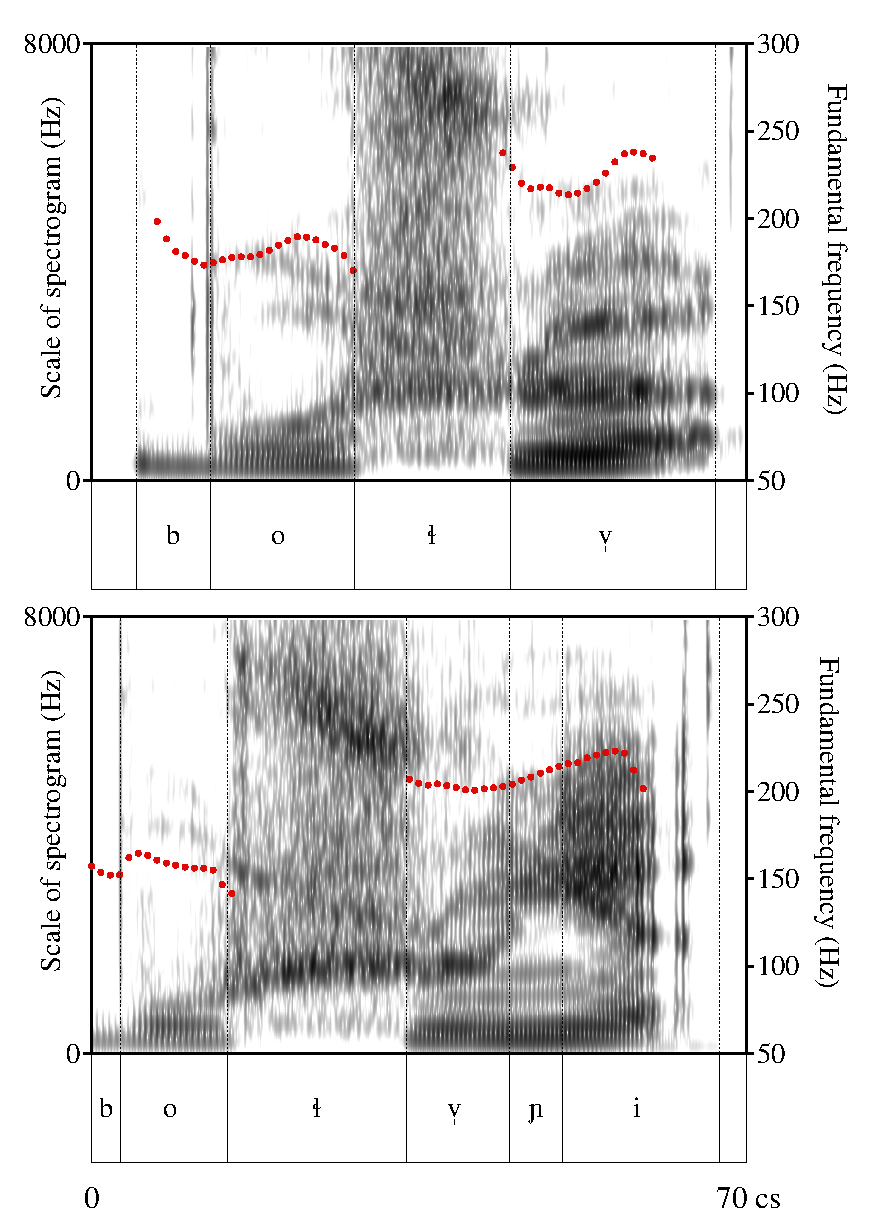
\includegraphics[width=.70\textwidth]{figures/PigBrains/PigBrains.eps}
\caption{\label{fig:spectrogramandf0tracingoftwonaphrases}Spectrogram and F\textsubscript{0} tracing of  ‘pig’s brains’ and ‘is \mbox{(a/the)} pig’s brains’.}
\end{figure}


The clear rise in F\textsubscript{0} on the rhyme /\ipa{v̩}/ in the top part of the figure is consistent with
phonological description as a~MH tone; and the flatter shape on the same rhyme in the bottom part
of the figure, followed by higher F\textsubscript{0} on the \isi{copula}, is consistent with phonological description as
a~sequence of M on one syllable and H on the next. But there is no way to read phonological tones off F\textsubscript{0}
tracings (as emphasized e.g.~by \citealt{cruzetal2014} and \citealt{morey2014}). \figref{fig:spectrogramandf0tracingoftwonaphrases} illustrates a~phenomenon that is immediately apparent when examining any
piece of \is{experimental phonetics|textbf}experimental evidence: variability in the realization of tone. For instance,
glottalization, which is common in Yongning Na in utterance"=final position, is found at the end of both tokens, exerting a~lowering influence on F\textsubscript{0}
towards the offset of voicing. (In these materials, the phrases /\ipa{bo˩-ɬv̩˧˥}/ ‘pig’s brains’ and /\ipa{bo˩-ɬv̩˧ ɲi˥}/ ‘is
(a/the) pig’s brains’ are both found in absolute final position, and therefore constitute entire sentences on
their own.) Also, /\ipa{bo˩}/
‘pig’ is realized with noticeably different F\textsubscript{0} in the top part of the figure and in the bottom
part. Tone levels have some range of \isi{variation} within tonal space (F\textsubscript{0}), in the same way as vowels have some
range of \isi{variation} within the acoustic space (as characterized essentially by the first three
formants, F1-F2-F3). In Yongning Na, rising tones are never found in initial position within a~tone
group, and hence the identification of an~initial L tone (as on the syllable /\ipa{bo˩}/ ‘pig’) is not jeopardized
by its realization with a~slight rise, as in the top part of \figref{fig:spectrogramandf0tracingoftwonaphrases}. Seen in this light, the
existence of slightly rising allotones (allophones of the tones) does not come as a~surprise: it makes sense in view of the
state of the phonological system, in the same way as, in a~language that does not have contrastive aspirated
consonants, plain (unaspirated) unvoiced consonants may sometimes be realized phonetically with some
aspiration.

Back in the 1970s, at a~time when F\textsubscript{0} tracings were difficult to do, necessitating expert technical skill, a~specialist in Bantu tone asked a~phonetician to create an~F\textsubscript{0}
tracing from a~recording illustrating a~specific phonological phenomenon. After receiving the
desired tracing, this famous specialist of tonology said that there must be a~mistake, as the F\textsubscript{0}
tracing did not correspond to the tone pattern that his trained ear discerned clearly in the
recording. In fact, there was no error in F\textsubscript{0} detection: the issue lay in this colleague’s
expectation of a~neatly binary F\textsubscript{0} tracing, straightforwardly reflecting the phonological tone
sequence (J. Vaissière, p.c.\ 2001). Experimental examination of spoken language reveals that, even in languages with
relatively straightforward prosodic systems, such as Standard \ili{Japanese}, F\textsubscript{0} curves are shaped by
a~number of factors, and do not reflect phonological tone in a~crystal"=clear, transparent
way. Without the help of a~language consultant, it is simply impossible to know for sure for a~given
utterance that has, for instance, a~lowering of F\textsubscript{0} on its last
syllable, whether this is due to a~L tone on that syllable or to intonational final lowering of
a~M-tone syllable. Arriving at tonal contrasts requires factoring out \isi{intonation}, and vice versa.


The following sections present salient characteristics of Na \isi{intonation}. But first some concepts need
to be discussed.




\subsection{Definition of terms}
\label{sec:definitionofterms}

\is{prosody|textbf}Prosody as defined here consists of (i)~lexically distinctive properties: stress, as in
\ili{English}; tone, as in \ili{Mandarin}, Yorùbá or Na; tonal accent, as in \il{Japanese|textbf}Japanese\footnote{As mentioned in \sectref{sec:adiscussionofalternativeformulations}, several competing analyses of the prosodic systems of {Japanese} dialects have been proposed (for a~review, see \citealt{kawahara2015}). The concept of tonal accent, also called pitch accent, has been presented by \citet{hymanhownot2009} as a~typical example of how \textit{not} to do prosodic typology: the argument is that “alleged pitch"=accent systems freely pick"=and"=choose properties from the tone and stress prototypes, producing mixed, ambiguous, and sometimes analytically indeterminate systems which appear to be intermediate”. However, the description of pitch"=accent systems as “intermediate” between stress and tone does not greatly clarify the issue. Hyman's questioning of pitch accent as a~typological category could be extended to tone, in view of the considerable heterogeneity of prosodic systems that have been described as “tone systems” (see \citealt{brunelleetal2016} and the discussion
	 in \sectref{sec:typologicalbackgroundtotheclassificationofyongningnatonesasleveltones}). As Hyman underlines, the goal of prosodic typology should be to classify not languages but rather the properties of their subsystems. In the present state of prosodic typology, it is not obvious to me that there is much to gain from prohibiting tonal accent as a~descriptive label.} and Swedish;
phonation"=type register, as in Mon (\il{Mon-Khmer}Mon"=Khmer family); (ii)~\isi{intonation}; and (iii)~performance
factors, including rhythm.

\is{intonation|textbf}Intonation is often identified with the parameters in which
it is manifested~-- and especially with fundamental frequency. But this identification is inappropriate, because intonation is a~complex, abstract
structure. It can usefully be divided into (i)~two sub"=systems of linguistic structure: syntactic
\isi{intonation} \textit{(\isi{phrasing})}, which essentially reflects syntax in the broader sense, and pragmatic
\isi{intonation} \textit{(prominence)}, which reflects \isi{information structure}, and (ii)~attitudinal and emotional
dimensions, which convey speaker attitudes and emotions. This view of \isi{intonation} is shown in \figref{fig:intonation}. It needs to be emphasized that this embedded (tree"=like) graph is a~highly simplified representation: its aim is to provide a~visual recapitulation of the basic distinctions made here. It does not aim to reflect the delicate links among the various components of \isi{prosody}, e.g.~between rhythm and lexically distinctive suprasegmentals.

\begin{figure}[ht]
	\centering
	\begin{tikzpicture}
%	\node (a) at (0, 1) {\textsc{gen/num (erg)}};
	\node (b) at (1.5, 1.5) {\is{phrasing}Phrasing};
%	\node (c) at (1.5, 2.5) {\textsc{gen/num (erg)}};
	\node (d) at (0, 2.75) {Lexically distinctive properties};
	\node (e) at (3.5, 1.5) {Prominence};
%	\node (f) at (3, 1) {\textsc{gen/num (erg)}};
	\node (g) at (4.5, 2.75) {Intonation};
	\node (g2) at (8.2, 2.75) {Performance factors};
	\node (h) at (5.5, 1.5) {Attitudes};
	\node (i) at (7.5, 1.5) {Emotions};
%	\node (j) at (6, 1) {\textsc{gen/num (acc)}};
%	\node (k) at (9, 1) {\textsc{person (acc)}};
%	\node (l) at (9, -0.5) {Past \textit{\textbf{(Past Imperfect)}}};
%	\node (m) at (9, -1) {\textsc{person (acc)}};
	\node (n) at (3.5, 4) {Prosody};
	\foreach \from/\to in {g/h, g/i, n/d, n/g, g/b, g/e, n/g2}
	\draw [<-] (\from) -- (\to);
	\end{tikzpicture}
	\caption{A highly schematic representation of the components of {prosody}.}
		\label{fig:intonation}
\end{figure}

%\begin{figure}[h!]
%	\caption[{A highly schematic representation of the components of \isi{prosody}.}]{A highly schematic representation of the components of \isi{prosody}.}
%
%\begin{tikzpicture}
%
%[sibling distance=10em,
%every node/.style = {shape=rectangle, rounded corners,
%	draw, align=center,
%	top color=white, bottom color=blue!20}]
%
%\node {prosody} % 1st level. No need for closing.
%		child { node {lexically distinctive properties} %2nd level, 1st branch OPENED
%%					child { node {tone (as in Na)} }
%%					child { node {stress (as in \ili{English})} }
%%					child { node {tonal accent (as in \ili{Japanese})} }
%%					child { node {phonation"=type registers (as in Mon)} }
%			} % 2nd level, 1st branch CLOSED
%		child { node {intonation} %2nd level, 2nd branch OPENED
%%					child { node {linguistic\\ structuration\\ systems} %3rd level, 1st branch
%						child { node {phrasing} }
%						child { node {prominence} }
%					%		child { node {center} } }
%%					 } % %3rd level, 1st branch CLOSED
%%				 	child { node {attitudinal\\ and\\ emotional\\ dimensions}  %3rd level, 2nd branch OPENED
%				 		child { node {attitudes} }
%				 		child { node {emotions} }
%				 		%		child { node {center} } }
%%				 	} %3rd level, 2nd branch CLOSED
%				child { node {performance\\ factors} }
%		; % semicolon to close the list of nodes
%
%\end{tikzpicture}
%\end{figure}

These definitions, taken from a~publication about prosodic constituents in \ili{French}
\citep{vaissiereetal2006}, elaborate on proposals which (in my view) are similar in their essentials
\citep{coustenobleetal1937,delattre1965,martin1977b,rossi1999}. Usage
still varies considerably among authors (a detailed discussion of various frameworks is proposed
by \citealt{dicristo1998}).

As defined here, tone has the function of lexical and morphological differentiation, and
\isi{intonation} has the functions of (i)~speech \isi{phrasing}, (ii)~coding prominence, and (iii)~expressing emotions and attitudes towards the listener. Intonation is, in Bolinger’s phrase, a~“half"=tamed savage”
\citep[475]{bolinger1978}. \textit{Phrasing} is on the tamer, more intellectual side; it surfaces at
its clearest in deliberate oral renderings of elaborately composed texts. \textit{Prominence} is
a~less tame dimension of \isi{intonation}: it can still be described in terms of a~linguistic system, with
clear cross"=linguistic differences, but the intrusion of the stronger manifestations of prominence
can interfere with \isi{phrasing} as determined by syntactic structure. The expression of attitudes
and emotions can partly be described in terms of ethological principles, such as the Frequency Code:
 
\begin{quotation}
{\dots}~an innately specified ‘Frequency
Code’ ({\dots}) associates high acoustic frequency with the primary meaning of ‘small vocalizer’ and thus secondary meanings as ‘subordinate, submissive, non threatening, desirous of the receiver's goodwill, etc.’ and associates with low acoustic frequency the primary meaning of ‘large vocalizer’ and such secondary meanings as ‘dominant, aggressive, threatening’, etc.~ \citep[1]{ohala1984}.
\end{quotation}
	
The phrase “syntactic \isi{intonation}” may appear to be somewhat of a~misnomer, insofar as intonational \isi{phrasing} does not stand in a~strict, one"=to"=one relationship with syntactic units, as was
already noted in the early classics of phonetics \citep{grammont1933} and confirmed by later work
(\citealt{selkirk1972}; \citeyear[231]{selkirk2000}; \citealt{martin1981}). The phrase “syntactic
\isi{intonation}” is nonetheless retained in view of the fact that knowledge of a~sentence’s syntax offers
a~sufficient basis for the synthesis of an~acceptable fundamental frequency {contour}
\citep{vaissiere1971}.

The acoustic correlates of \isi{prosody} are many. They include the variations in fundamental frequency,
\isi{duration} and intensity and \is{phonation types}phonation type, but also the allophonic variations in the realization of
the phonemes. Thus, \isi{prosody} has correlates at the respiratory level (i.e.\ the subglottal level), at the glottis,
and at the supra"=glottal level (see \citealt{erickson1998}). All parameters take part in \isi{prosody} simultaneously, to a~greater or
lesser extent.

Lastly, here are some clarifications about the concepts of ‘\isi{tone sandhi}’, ‘morphotonology’ and ‘tonal morphology’. \is{tone sandhi|textbf}\textit{Tone sandhi} refers to phonologically specified tone change, applying automatically inside a~given phonological domain. To put it differently, \textit{tone sandhi} refers to categorical phenomena of tone change conditioned by the phonological context. The seven tonal rules of Yongning Na presented in \sectref{sec:alistoftonerules} (repeated below) are \isi{tone sandhi} rules, in the sense that they govern adjustments among neighbouring tones within a~given phonological domain (the \isi{tone group}).

	\begin{enumerate}[leftmargin=2cm, itemsep=0pt, labelwidth=\widthof{Rule~1:}]%[topsep=12pt, partopsep=0pt]
		\item[Rule~1:] L tone spreads progressively (“left"=to"=right”) onto syllables that are unspecified for tone.
		\item[Rule~2:] Syllables that remain unspecified for tone after the application of Rule 1 receive M tone.
		\item[Rule~3:] In tone"=group"=initial position, H and M are neutralized to M.
		\item[Rule~4:] The syllable following a~H-tone syllable receives L tone.
		\item[Rule~5:] All syllables following a~H.L or M.L sequence receive L tone.
		\item[Rule~6:] In tone"=group"=final position, H and M are neutralized to H if they follow a~L tone.
		\item[Rule~7:] If a~\isi{tone group} only contains L tones, a~post"=lexical H tone is added to its last syllable.
	\end{enumerate}

\textit{Morphotonology} refers to categorical change in tone governed by rules that are confined to specific syntactic phrase types, e.g.~the different rules that apply to object plus verb, subject plus verb, numeral plus classifier, and so on. 

Finally, \textit{tonal morphology} refers to grammatically specified tone change marking certain morphosyntactic categories. The phrase “tone cases” is used in the description of some \ili{Bantu} languages, such as UMbundu \citep{schadeberg1986tone}, where a~noun's tone changes according to its case. 
%No less than twenty"=five African languages that have tone cases are listed (and plotted on a~map) by \citet[225]{konig2008case}. 
The addition of a~certain tone to verbs can express a~given tense/aspect/modality category. 
%Tonal morphology can further be divided into \textit{concatenative} and \textit{derivational} types. Concatenative tonal morphology consists in the addition of “tonal morphemes” (on the case of Saramaccan: \citealt{good2002, good2004}). 

In Yongning Na, there is no tonal morphology, in the sense that there are no tonal morphemes. The \is{floating tone}floating High tone in Yongning Na is not a~morpheme (the combination of a~form and a~meaning): it is one of the lexical categories of nouns. As a~consequence, only the first two of the three concepts characterized above~-- \is{tone sandhi}sandhi, morphotonology, and tonal morphology~-- are relevant to the present study. 

Some authors prefer “a broad and loose usage of the term” \textit{sandhi} covering both \is{tone sandhi}sandhi and morphotonology as defined here \citep[x]{chen2000}. But while it is advisable to cast the net wide in language surveys \citep[such as the survey of Chinese dialects by][]{chen2000}, the distinction between sandhi and morphotonology is crucial to the present study. The reason for writing a~book"=length description is that tonal changes in Yongning Na are not simply a~matter of phonology: in addition to sandhi (as defined here: a~phonological phenomenon), Yongning Na has a~host of syntactically restricted \is{tone rules}tone rules, i.e.\ morphotonology. 


\subsection[About tools for intonational transcription]{About tools for intonational transcription}
\label{sec:theabsenceoffullysatisfactorytoolsforintonationaltranscription}

There does not yet exist a~standardized system for transcribing \isi{intonation}. This is easy to
understand in view of the intricacy of this linguistic domain, described above. 

\begin{quotation}
	Since Bolinger first raised the {question} explicitly in \citeyear{bolinger1951}, there has been considerable argument over whether \isi{intonation} is better described as pitch contours, like the kinetic tones of the British tradition, or as a~sequence of pitch phonemes or significant levels (the American approach exemplified by \citealt{pike1945}, \citealt{wells1945}, \citealt{trageretal1951}, \citealt{hockett1955}, and now \citealt{liberman1975} and the autosegmental school originated by \citealt{goldsmith1976}). \citep[531]{ladd1978}
\end{quotation}

%Command \noindent added to avoid having an indent. Proofreader suggestion: since this sentence continues the argument, it is better not to indent. 
{\noindent}Under the second of these approaches, \isi{intonation} is modelled by means of discrete levels, as if it were tonal. This approach is known as “autosegmental"=metrical”, and has dominated
discussions of \isi{intonation} since the 1980s. A~reason for its popularity is that it seemed to hold promise for implementation in speech synthesis \citep{pierrehumbert1981} and prosodic annotation \citep{silvermanetal1992}. The basic tenets of “autosegmental"=metrical” models are concepts borrowed from autosegmental tonology, such as level
tones, \isi{downstep} and tone \is{tone spreading}spreading. Pitch accents, organized in a~linear sequence, are considered the building blocks of an \isi{intonation} {contour} (see the textbooks by \citealt{ladd1996} and \citealt{gussenhoven2004}, for instance).

If one stands back to take a~global view of tonal models of \isi{intonation}, however, they appear as hybrid and
somewhat perplexing systems (as pointed out by \citealt{martin2001} and \citealt{wightman2002}). The posited ‘intonational tones' are abstract
entities, but the labels are also used as a~system for phonetic transcription of linguistically
significant aspects of F\textsubscript{0} curves as they are observed. Tonal labels tend to be assigned by eye (on the basis of F\textsubscript{0} curves superimposed on spectrographic displays) more than by ear,
whereas ‘\isi{boundary tone}s' are meant to reflect the perceived cohesion between successive words, and
are thus grounded in aural impressions as well as on the observation of F\textsubscript{0} curves. “To be fair to the original spirit of Janet Pierrehumbert, who intended to describe
American \ili{English} and carefully avoided generalization in her thesis, applying ToBI symbols to a~new
language requires prior re"=evaluation of the underlying principles” \citep{vaissiere2002}.

Interestingly, before he became one of the proponents of “autosegmental"=metrical” models, Bob Ladd expressed the conviction that he had “clearly demonstrate[d] the inadequacy of any approach to \ili{English} \isi{intonation} which treats contours as sequences of significant pitch levels” \citep[517]{ladd1978}.

\begin{quotation}
	In short, linguistic systems force users to identify certain signals as discretely different from one another; and linguists' analyses should reflect these discrete differences. But an analysis of \isi{intonation} in terms of pitch levels forces us to distinguish points along a~gradient as also being discretely different~-- even though they are not~-- because the theory provides no principled way of knowing when changing a~certain feature in a~sequence is going to produce a~‘modulation’, and when it is going to produce a~‘very different tune’. No amount of tinkering with theoretical mechanisms can remedy this defect; the best that any pitch-level theory can do is ignore it. To continue to ignore the difference between the gradient and the all"=or"=none by forcing it into a~pre"=ordained system of distinctions is only to put off reaching an understanding of how \isi{intonation} really functions in language. \citep[539]{ladd1978}
\end{quotation}

%Command \noindent added to avoid having an indent. Proofreader suggestion: since this sentence continues the argument, it is better not to indent. 
{\noindent}This strand of thought (which makes excellent sense to me) continued to be pursued by some scholars even during the heyday of “autosegmental"=metrical” models. Alternatives to tonal models of \isi{intonation} include the Kiel Intonation Model and its developments
\citep{niebuhretal2004,kohler2005,niebuhr2007,Niebuhr2010}, superpositional approaches
\citep{vaissiere2002,vaissiere2004,gronnum1991,gronnum1998a,gronnum1998b,lindau1986}, and various others \citep{delattre1966a,fonagy1989,rossi1999,martin1977b,martin2015,hirstetal1998b}. These approaches are currently
outside the mainstream of \isi{intonation} studies, in the same way as non"=autosegmental analyses of tone
systems fall outside mainstream (generative) phonology (some reflections on this situation are set
out in \citealt{zerbian2010,michaudetal2015f}). My evaluation of the available evidence is
that tonal accounts of \isi{intonation} in tone languages run into considerable difficulties, and that it
is better to adopt a~vocabulary which suits the data, even if it is not mainstream at present,
rather than force the data into inadequate models. As a~consequence, the
present description adopts a~functional
perspective that clearly distinguishes tone and \isi{intonation}.

Another distinction which is essential to \isi{prosody} studies is that between an~abstract level of description, on the one hand, and the level of phonetic realizations, on the other. This distinction is threatened in frameworks where ‘tone’
  is considered synonymous with F\textsubscript{0}. For instance, \citet{hymanetal2008b} define the term ‘tonal’ in a~phonetic sense, to mean
  ‘realized by F\textsubscript{0}’, and ‘non"=tonal’ to mean ‘realized by parameters other than F\textsubscript{0}’ (such as
  phonation types). The equation between ‘tone’ and ‘F\textsubscript{0}’ appears so self"=evident that it could seem unnatural to try to define tone in any different
  way. But from a~classical linguistic perspective, it is crucial to make a~distinction between
  F\textsubscript{0}, which is an~acoustic parameter, and linguistic tone, which is a~functional concept.


\subsection{Intonation in level"=tone languages: A~review}
\label{sec:literaturereviewintonationintonallanguages}

In addition to the above remarks about the definition of terms and the frameworks for studying \isi{intonation}, it may be useful, before beginning to describe \isi{intonation} in Yongning Na, to review studies of \isi{intonation} in other level"=tone languages. This review also paves the way for the typological analyses set out in a later chapter (\sectref{sec:typologicalperspectives}).

Auditory observations on phonetic realizations of tone in a~two"=tone language (Lingala) are proposed by \citet{guthrie1940}:

\begin{quotation}
	{\dots}~the only possible variations in the \isi{intonation} of a~word or sentence are these: 
	\begin{enumerate}[itemsep=0pt, topsep=0pt, partopsep=0pt, parsep=0pt]
	\item[(a)] A~widening or narrowing of the interval between the high and the normal tones.
	\item[(b)] A~raising or lowering of the pitch of voice, i.e.\ a~change of key.
	\item[(c)] A~gradual rise or fall of the pitch of voice, i.e.\ a~continuous change of key.
	\end{enumerate}
	In Lingala the only two variations that seem to exist are (a) and (b). The gradual fall of the pitch of the voice during a~sentence is so slight as to be almost imperceptible. There is, however, another modification which affects the last syllable of a~phrase or sentence only. This may be called the final cadence, and means that a~high tone becomes a~high"=falling, while a~tone that is normal becomes normal falling to low. \citep[472--473]{guthrie1940}
\end{quotation}

Parameter (a) is considered to possess three degrees of \isi{variation}. Guthrie proposes that there are four phonetic ranges, for which~-- somewhat surprisingly for 21\textsuperscript{st}"=century readers~-- he brings in musical definitions: minor third (considered as the “normal range''), major third, major fourth, and major fifth. Interestingly, Guthrie believes that the tonal range is set at sentence level. This arguably reflects a~characteristic of the language that he was examining (Lingala): successive level tones hang together much more closely than in \is{complex tones}complex"=tone systems,\footnote{On the typological distinction between level"=tone systems and complex"=tone systems, see \sectref{sec:typologicalbackgroundtotheclassificationofyongningnatonesasleveltones}.} where attention is drawn to \textit{local} phenomena of F\textsubscript{0} \isi{range expansion} or compression, which do not change the phonological nature of the tone of the syllables at issue. 

To venture an~impressionistic description of the difference between the two types of systems: level tones make sense as part of a~sequence, whereas phonetically \is{complex tones}complex tones each have a~stronger identity. Level tones are subject to a~range of categorical processes that modify the tonal string, such as tone \is{tone spreading}spreading (a~H or L tone getting copied onto successive syllables), whereas \is{complex tones}complex tones are less prone to categorical change, and more prone to noncategorical, local intonational modification conveying indications about emphasis and \isi{phrasing}. This does not entail that successive complex tones are independent of one another. For instance, in \ili{Mandarin}, focus placed on one syllable has consequences on neighbouring~-- especially on following~-- syllables: “focus is usually related to F\textsubscript{0}-range"=expansion of focused words that are not in the final position of an~utterance and F\textsubscript{0}-range"=suppression of post"=focus words'' \citep[449]{zhangetal2004}. Moreover, tonal \isi{coarticulation} phenomena in \ili{Sinitic}, \ili{Vietnamese} or \ili{Thai} are strong, and they tend to harden diachronically into \is{tone sandhi}sandhi patterns \citep{abramson1979a, gandouretal1992, brunelle2003, brunelle2009b, zhangetal2011}. So it would not make sense to view the noncategorical intonational modification of complex tones as a~purely local phenomenon, or conversely, to consider that level tones cannot be subject to any local, noncategorical intonational modification. Still, the following generalization seems to hold: in the field of \isi{intonation} studies, Bantuists' attention seems to be regularly drawn to sentence"=level phenomena, rather than to local phenomena of pragmatic emphasis. This suggests that local variations of the sort observed in complex"=tone systems (as exemplified by \ili{Vietnamese}, \ili{Thai} and \ili{Sinitic}), where they do not affect the phonological nature of the tones, are not as salient in level"=tone systems as exemplified by \ili{Bantu} languages. When studying \ili{Bantu} \isi{prosody}, attention is drawn instead to \textit{categorical} local changes (changes that modify the string of phonological tones), and (secondarily) to sentence"=level phenomena. Echoing Guthrie's study about Lingala, a~study of Chichewa \isi{intonation} likewise focuses on sentence mode, specifically on the differences in F\textsubscript{0} between questions and statements \citep{myers1996}.
% : questions have a~final rise; they do not display the strong \isi{downdrift} found in statements; and they are produced in a~higher pitch range than statements

Guthrie describes the \isi{intonation} of Lingala in terms of five different levels. 
\begin{quotation}
	Although there are actually five different levels used the language remains essentially two"=tone, as in learning forms the only thing to be noticed is whether any syllable has a~high or a~normal tone. It is, moreover, interesting to notice how regular is the system of tone ranges. Emphasis shifts the \isi{intonation} to the next higher range. Interrogation move the tones two ranges higher, while the use of the subjunctive reduces the pitch to the next lower range. \citep[475--476]{guthrie1940} 
\end{quotation}

Description of \isi{intonation} in terms of a~finite number of levels was a~trend of the time in American structuralist approaches to \isi{intonation}. Analyses of \ili{English} \isi{intonation} published shortly after Guthrie's study assume that there are four relevant levels of pitch: extra high, high, mid and low \citep[42]{pike1945, trageretal1951}. In Trager \& Smith's system, the four levels combine with four relevant levels of stress (primary, secondary, tertiary, and weak), yielding a~symmetrical system of no fewer than sixteen “pitch allophones''. This system is rather contrived, and the sixteen units' links to linguistic functions look really tenuous. Fortunately, Trager \& Smith's proposal is about \ili{English}, and informed native speakers have provided articulate critical feedback: 

\begin{quotation}
	{\dots}~this reviewer, at least, simply does not hear the neatly symmetrical distribution of pitch allophones with phonemes of stress as Trager and Smith describe it, he often hears nothing to justify the writing of \textit{plus} junctures where his colleagues write them, he is sometimes in serious doubt whether to write primary or secondary stress, and he is openly astonished at the apparent claim by Trager and Smith that in final position they can distinguish four allophones of each of four pitch phonemes before each of three terminal junctures. ({\dots}) Readers dislike being told that they can ‘easily supply other examples' when the most patient effort leaves them utterly baffled. \citep{sledd1955} 
\end{quotation}

%Command \noindent added to avoid having an indent. Proofreader suggestion: since this sentence continues the argument, it is better not to indent. 
{\noindent}Writing about \isi{intonation} in Yongning Na is a~bigger scientific responsibility, as few native speakers are likely to examine the linguist's claims in such detail. 

A general issue with the framework proposed by Trager \& Smith to study \isi{intonation} is that it suffers from the same immoderate ambition as Hall \& Trager's framework for the \textit{analysis of culture}: “a hypothesis and methodology for the analysis of culture as a~whole and specific cultural systems{\dots} a~general analytic scheme into which all cultural activities, at all levels of integration and complexity, can be fitted'' \citep[57]{halletal1953}. By contrast, Guthrie's proposals have much to commend them. Guthrie clearly distinguishes the two level tones from the intonational factors that influence their realization. Moreover, although the four proposed phonetic ranges are presented in an~order based on form, from narrowest to widest, the analysis hinges on the linguistic functions associated with variations in tone range. This is a~fruitful approach, which brings out a~wealth of interesting observations. 

Less positively, Guthrie's proposal that the tonal levels constitute a~closed set (five in all) is hard to reconcile with the observed diversity of intonational patterns. It is understandable that linguists should wish to operate with a~finite set of basic units in all fields of linguistic description, as they do at the phonemic level, and in the study of tonal phenomena. But these tools are less than fully appropriate in the field of \isi{intonation}; linguistic models that treat \isi{intonation} systems on the {analogy} of phonemic systems fail to capture their object.
\begin{quotation}
	This phenomenon [=\isi{intonation}] has considerable importance in oral communication, but has specificities that make it really troublesome to the linguist, since the methods that have been tried and tested in other areas do not seem truly adequate for the analysis of \isi{intonation}. \citep[173]{creissels1994}\footnote{\textit{Original text}: L'importance de ce phénomène [=l'{intonation}] dans la communication orale est considérable, mais sa spécificité gêne beaucoup le linguiste, car les méthodes d'analyse qui ont fait leurs preuves dans d'autres domaines ne semblent pas convenir vraiment pour l'analyse de l'{intonation}.}
\end{quotation}

It now seems clear that there is no cross"=linguistically fixed number of levels to be distinguished when representing phonetic realizations of tone. On the basis of expert listening, Creissels proposes stylized representations of the phonetic realizations of certain sequences of tones (in a~two"=tone system) which clarify that tone implementation is language"=specific. For instance, \figref{fig:notes} illustrates an~observation made in some tonal languages of Subsaharan Africa: the first in a~sequence of L tones following a~H tone carries pitch that is intermediate between that of the preceding H tone and that of the following L tones. ``Such realizations can be seen as the inception of a~phenomenon of propagation: if the raising of the first in a~sequence of L tones following a~H tone becomes more noticeable, it can result in \isi{misperception} as a~H tone'' \citep[215--216]{creissels1994}.\footnote{\textit{Original text}: On observe par exemple dans certaines langues que, sans que son identification comme ton bas soit remise en cause, le premier d'une séquence de tons bas succédant à un ton haut est réalisé à un niveau intermédiaire entre celui du ton haut qui le précède et celui des tons bas suivants. ({\dots}) On peut voir dans de telles réalisations l'amorce d'un phénomène de propagation~: en effet, si le réhaussement du premier d'une séquence de tons bas succédant à un haut s'accentue, on peut aboutir à la confusion avec un ton haut ({\dots}).}

%\begin{figure}[t!]
%To place it exactly here: [h!]
\begin{figure}
\centering
\caption{Stylized representation of the realization of a~H.L.L sequence in some Subsaharan languages: as a~gradual decrease in pitch from the first syllable to the third \citep[217]{creissels1994}.}
\begin{tikzpicture}
\draw (0,0) -- (4,0);
\draw (0,-0.5) -- (4,-.5);
\draw (0,-1) -- (4,-1);

\draw[fill=white] (1,0) circle (2pt);
\draw[fill=white] (2,-0.5) circle (2pt);
\draw[fill=white] (3,-1) circle (2pt);

\draw (1,-1.5) node {ó};
\draw (2,-1.5) node {ò};
\draw (3,-1.5) node {ò};
\end{tikzpicture} 
\label{fig:notes}
\end{figure}

This observation brings out the tonal \isi{coarticulation} pattern's evolutionary potential. On the other hand, readers with an~interest in \is{experimental phonetics}experimental phonetics may want more detail than the schematized representation in \figref{fig:notes} can encapsulate. If there are three L tones in a~row, are the second and third realized on the same phonetic level? Or is there gradual decrease in pitch from one syllable to the next? Is this decrease linear or asymptotic? Experimental"=phonetic studies of level tones containing proposals for modelling tonal implementation are available for several two"=tone systems, such as Dinka
\citep{remijsenetal2008}, Kinyarwanda \citep{myers2003} and Sotho
\citep{zerbianetal2010a,zerbianetal2010b}, three"=tone systems
(\citealt[48--65]{teo2014}; \citealt[100--106]{coupe2003};
\citealt{laniranetal2003}), and four"=tone systems, e.g.~Mambila
\citep{connell2003, connell2016}. These studies confirm that issues of tone realization are conditioned by a~host of language"=specific parameters. 

The present chapter aims to bring out such parameters of the Yongning Na prosodic system. No experimental phonetic tools are deployed to explore these issues: ``the linguistic analysis, which may perfectly well be made on auditory basis, must come first'' \citep[4]{fischer1949}. The prospect of future experimental\is{experimental phonetics} verification was constantly kept in mind, however, and the observations proposed below are intended as a~basis for phonetic experiments.

\section{Syntactic intonation: Phrasing and junctures}
\label{sec:syntacticintonationphrasingandjunctures}

The most important unit in the prosodic organization of Na speech is the \isi{tone group}, studied in Chapter~\ref{chap:toneassignmentrulesandthedivisionoftheutteranceintotonegroups}. But from the
point of view of phonetic implementation, successive tone groups are not entirely independent. Tone
groups are part of higher"=level prosodic units which can be defined in various ways. Two units
which appear especially useful as cross"=linguistic descriptive concepts, though their definition is
not without problems, are the prosodic paragraph and the sentence (also referred to as
‘utterance’, with a~view to bringing out its grounding in a~communicative context, emphasized e.g.~by \citealt{culioli1995}). The term ‘paragraph’ is open to criticism on the part of linguists who object
to the transfer of concepts from the study of written texts to that of oral speech; it is
a~convenient term nonetheless, in view of the similarities between the division of a~written text
into paragraphs and that of speech into prosodic paragraphs, with a~high degree of \is{stylistics}stylistic freedom in both cases. Here is a~brief characterization of the prosodic paragraph and the sentence, adapted from \citet[50–52]{vaissiereetal2006}.

Cross"=linguistically, the peak F\textsubscript{0} value in a~sentence tends to decrease from the
first to the last sentence in a~paragraph \citep{lehiste1975}. The end of the paragraph typically
ends on an~extra"=low F\textsubscript{0} (often leading to a~change in phonation
type) and intensity. 

At sentence level, the neutral, affirmative sentence is the basic,
archetypal pattern from which other sentence modes depart \citep{thorsen1980}. Abstracting away from all other dimensions of \isi{prosody} (such as lexically distinctive suprasegmentals, prominence, and the expression of attitudes and emotions), the
F\textsubscript{0} curve for the sentence rises to a~peak located on one of the
sentence’s first syllables. In the course of the sentence,
a~phonetic, gradual, noncategorical decrease in fundamental frequency takes place. This is known as ‘\is{declination|textbf}{declination}’. Fundamental frequency therefore fluctuates within a~gradually narrowed
range. A~final lowering marks the end of the sentence. (This corresponds to Tune 1 as described for
\ili{English} by \citealt{armstrongetal1926}.) Final lowering is a~more local phenomenon, typically
affecting the last syllable in declarative utterances, but this is subject to cross"=language \isi{variation}.

\begin{quotation}
	Final lowering can be total, leading to the neutralisation of High and Low tones, as in Akan. It can be realized as a~low register plateau, as in Chi\-che\-wa or in Bemba (for the long stretched one), or as a~gradual fall, as in Embosi, or as a~sharp fall, as in Bemba (for the one syllable one). Its domain can be short (one syllable) or rather long (a stretch of tone bearing units). \citep[4-5]{downingrialland2016}
\end{quotation}

Declination and final lowering are common across languages, as is their suspension to convey
non"=assertiveness (in questions, or to convey nuances of doubt and uncertainty).

%In Yongning Na, \isi{declination} is most transparently observed in sentences that have long sequences of like tones: M..M or L..L.\footnote{Remember that H..H sequences are ruled out by the fact that H tone is culminative: there can be at most one H~tone in a~\isi{tone group}. All tones following H are depressed to L: see \sectref{sec:alistoftonerules}.}

From a~phonetic point of view, these phenomena interact with phonological tones: the phonetic
realization of a~phonological H, M or L differs considerably depending on the position of the
syllable inside the sentence and the prosodic paragraph. For instance, in Yongning Na the 1\textsuperscript{st}, 2\textsuperscript{nd} and 3\textsuperscript{rd}-person pronouns //\ipa{njɤ˩}//, //\ipa{no˩}//, and //\ipa{ʈʂʰɯ˥}// all have M tone \is{form!in isolation}in isolation due to the \isi{neutralization},
in this position, of the lexical categories L, M and H. Their surface phonological representation \is{form!in isolation}in isolation is therefore /\ipa{njɤ˧}/, /\ipa{no˧}/ and
/\ipa{ʈʂʰɯ˧}/, respectively. But in my first notes I transcribed them with H tone, as [\ipa{njɤ˥}],
[\ipa{no˥}] and [\ipa{ʈʂʰɯ˥}]. This was due to their realization on a~high pitch \is{form!in isolation}in isolation. In that
context, their pitch is noticeably higher than that of a~M tone in tone"=group"=initial position later
on inside a~prosodic paragraph.
% see, among other examples, the contrast between the phonetic realization of
%/\ipa{njɤ˧}/ ‘I’ and /\ipa{ə˧si˧}/ ‘grandmother’ in /\ipa{njɤ˧} {\kern2pt}|{\kern2pt}
%\ipa{ə˧si˧}/ ‘my grandmother’ in Dog.56. 

Moreover, since the opposition
between M and H is neutralized in tone"=group"=initial position, a~phonetically high realization
runs no risk of being misinterpreted by native listeners. As a~consequence, M tones in this
position have the entire upper part of the tonal phonetic space as their range of intonational
\isi{variation}. In my first field notes, I transcribed (\ref{ex:idonteat}) as $\ddagger${\kern2pt}\ipa{njɤ˥ mɤ˧-dzɯ˥}; I was led to
this phonologically inappropriate notation by the considerable phonetic difference in pitch between the first and
second syllables, and the similarity in pitch between the first and last syllables of this short
sentence.

\begin{exe}
	\ex
	\label{ex:idonteat}
	\ipaex{njɤ˧ {\kern2pt}|{\kern2pt} mɤ˧-dzɯ˥.}\\ 
	\gll njɤ˩	mɤ˧-	dzɯ˥\\
	\textsc{1sg}		\textsc{neg}		to\_eat\\
	\glt ‘I don’t eat.’
\end{exe}

These intonational facts had to be brought to light before a~correct transcription of the
surface phonological form of the pronouns could be arrived at. 


\section{Pragmatic intonation}
\label{sec:pragmaticintonation}

“Information structure is a~vast topic of research that has been pursued within different theoretical frameworks” \citep[244]{krifka2008}, and with different objectives in view. A~few general observations about \isi{information structure} in Yongning Na will be followed by a~discussion of three phenomena that belong to \textit{pragmatic intonation}: (i)~\isi{emphatic stress} (\sectref{sec:emphaticstressanditstoneddownavatars}), (ii)~\isi{focalization} through local intonational modification of tone (\sectref{sec:focalization}), and (iii)~intonational backgrounding of \isi{function words} (\sectref{sec:intonationalbackgroundingofparticles}).\footnote{This section contains passages adapted from \citet{michaudetal2016}.}

The following generalization about Qiang proposed by \citet[221]{lapollaetal2003a} also applies to Yongning Na (and other \il{Sino-Tibetan}Sino"=Tibetan languages): 

\begin{quotation}
	\begin{sloppypar} % To avoid overfull hbox
	The structure of the clause is to some extent affected by pragmatic factors, but this only applies to the order of noun phrases in the clause. The utterance-initial position is the unmarked topic position (though secondary topics can follow the primary topic), while the position immediately before the verb is the unmarked focus position, and so the focused element will generally appear there. The verb always appears in final position; there is no possibility for the actor of a~clause to appear in postverbal position, even if it is focal. The only \is{exceptions}exception to this is the occasional afterthought clarification of a~noun phrase that was omitted or expressed as a~\is{pronouns}pronoun in the clause.
	\end{sloppypar}
\end{quotation}

%Command \noindent added to avoid having an indent. Proofreader suggestion: since this sentence continues the argument, it is better not to indent. 
{\noindent}Information structure in Na has accordingly been described as ‘topic-comment’, extending an observation made by Chao Yuen-ren about \ili{Sinitic}: “the grammatical meaning of subject and predicate in a~\il{Sinitic}Chinese sentence is topic and comment, rather than actor and action” (\citealt[69]{chao1968}; see also \citealt{shi2000}; \citealt{lapolla2009}). 
\begin{quotation}
The primary \isi{information structure} in Na is topic/comment rather than subject/predicate. ({\dots}) [A]~topic can be a~nominal argument, which the rest of the sentence will comment upon, but the topic can also be an {adverbial}, an independent clause, or a~dependent clause. \citep[296]{lidz2010}
\end{quotation}

Example (\ref{ex:stomachache}) provides an illustration. 

\begin{exe}
	\ex
	\label{ex:stomachache}
	\ipaex{le˧-dzɯ˥ {\kern2pt}|{\kern2pt} bi˧mi˧ go˩.}\\ 
\gll le˧-			dzɯ˥		bi˧mi˧			go˩\textsubscript{a}\\
\textsc{accomp}		to\_eat 		stomach/belly 		to\_ache\\
  \glt ‘[If] [you] eat [of it], [your] stomach [will] hurt!’ (Field notes. Context: on the mountain, pointing out a~berry that is not edible.)
\end{exe}


\subsection{Emphatic stress and its toned"=down avatars}
\label{sec:emphaticstressanditstoneddownavatars}

\is{emphatic stress|textbf}

An ‘up’ arrow \ipa{↑} is used to mark \isi{emphatic stress}, as in (\ref{ex:theelderwasaboy}), following a~convention used by \citet{mazaudon2004}. In Mazaudon's transcriptions of \ili{Tamang}, tone is indicated to the left of the syllable, and the mark for intonational emphasis is added to the right; for Yongning Na, since tone is indicated to the right of the syllable, the arrow \ipa{↑} indicating \isi{emphatic stress} is placed to the left of the syllable that carries it.

\begin{exe}
  \ex
  \label{ex:theelderwasaboy}
  \ipaex{tʰi˩˥, {\kern2pt}|{\kern2pt} ə˧mv̩˧ ʝi˥-hĩ˩ {\kern2pt}|{\kern2pt} -dʑo˩, {\kern2pt}|{\kern2pt} ↑zo˧ ɲi˥ tsɯ˩ {\kern2pt}|{\kern2pt} mv̩˩.}\\
  \gll tʰi˩˥		ə˧mv̩˧˥		ʝi˥ 	-hĩ˥		dʑo˥ zo˥ 		ɲi˩ 	tsɯ˧˥	mv̩˧\\
  then 	elder\_sibling	to\_do	\textsc{rel}	\textsc{top} boy/son 	\textsc{cop}
  \textsc{rep}	\textsc{affirm}\\
  \glt ‘The elder [of the two siblings] was a~boy.’ (Sister.5)
\end{exe}

In many contexts, \isi{emphatic stress} appears on a~constituent that can be predicted to receive normal focus \isi{prosody}. For example, in sentence (\ref{ex:theelderwasaboy}), one would expect the focus to be in the immediate preverbal position~-- the usual unmarked focus position for verb-final languages. Emphatic stress can be considered an extreme form of focus \isi{prosody}. It is an extreme along a~continuum: there is no hard-and-fast {boundary} between \isi{emphatic stress} and milder realizations of focus \isi{prosody}. 

Emphatic stress is phonetically located on one syllable only, but from the point of view of interpretation, there is ambiguity of focus marking: either “broad focus” or “narrow focus”, to use terms proposed by \citet{lambrecht1994}. This phenomenon is extensively studied in the literature on focus projection (e.g.~\citealt{selkirk1995}). 

The phonetic realization of \isi{emphatic stress} includes effects on the articulation of vowels and consonants. For instance, the second syllable of the verb /\ipa{dʑɤ˩↑bv̩˥}/ ‘to play’ is realized in (\ref{ex:playingwith}) with stronger trilling of the /\ipa{b}/ than is found in non-emphatic contexts. 
This can be considered an example of ‘articulatory prosodies’ in the sense of \citet{kohleretal2011} and \citet{niebuhr2013}.

\begin{exe}
	\ex
	\label{ex:playingwith}
	\ipaex{mv̩˩zo˩=ɻæ˩ lɑ˥ {\kern2pt}|{\kern2pt} ə˧ʝi˧-ʂɯ˥ʝi˩ {\kern2pt}|{\kern2pt} tʰi˩˥, {\kern2pt}|{\kern2pt} dʑɤ˩↑bv̩˥-ɲi˩ tsɯ˩ {\kern2pt}|{\kern2pt} mv̩˩!}\\
	\gll mv̩˩zo˩		=ɻæ˩		lɑ˧ 	ə˧ʝi˧-ʂɯ˥ʝi˩		tʰi˩˥		dʑɤ˩bv̩˥ 		-ɲi˩ 	tsɯ˧˥	mv̩˧\\
	girl	\textsc{associative}	with	long\_ago	so/then	to\_play		\textsc{certitude}
	\textsc{rep}	\textsc{affirm}\\
	\glt ‘The story goes that at that time, long ago, he would have fun [i.e.\ flirt] with girls!’ (Caravans.231)
\end{exe}


\subsubsection{Emphatic stress as a~language universal}
\label{sec:emphaticstressasalanguageuniversal}

Emphatic stress in Na appears to be essentially the same as in \ili{English} and \ili{French}, hence the choice
to use this label (proposed by \citealt{coustenobleetal1937}). Prototypical realizations of emphatic
stress have been shown to involve supplementary activity of the expiratory muscles, resulting in
a~sudden increase in subglottal pressure during the articulation of a~consonant
\citep{benguerel1973,cartonetal1976,ohala1978,Fantetal1996}, hence the term “force"=accent” used by \citet{kohler2003}. This category has been somewhat neglected in \isi{intonation} studies, as tonal models
of \isi{intonation} have led researchers to focus their attention mostly on the acoustic parameter of
fundamental frequency. But it is a~good candidate for the status of universal of human language. Its
linguistic functions range from the attitudinal and emotional to the pragmatic: it is the most
extreme manifestation of intonational emphasis. Toned"=down realizations of \isi{emphatic stress} are more common than its prototypical realization: physiological effort at a~subglottal level is mimicked through such strategies as
F\textsubscript{0} excursions and consonant \isi{lengthening}. Needless to say, the
description of \isi{emphatic stress} as a~language universal by no means implies that it is uniformly present in all
languages and all oral genres. Like other linguistic phenomena, it comprises important
language"=specific and speech"=style"=specific dimensions. Its frequency of use varies greatly from
language to language, from speaker to speaker, and from style to style; its \is{stylistics}stylistic effect is
inversely proportional to its frequency of use.


\subsubsection{The superposition of lexical tone and intonation}
\label{sec:thesuperpositionoflexicaltoneandintonation}


The general approach adopted here is superpositional, distinguishing different levels: in
particular, tone on the one hand, and intonational modifications (reflecting boundaries/junctures
and \isi{information structure}) on the other. Great care needs to be exercised in the analysis of these
phenomena, maintaining the functional distinction between lexical tones and \isi{intonation}. For
instance, when picking up the phone, speakers of \ili{Mandarin} say \textit{wèi} \zh{喂}, lexically a~tone-4 syllable, i.e.\ with sharply falling pitch; but in this context,
the lexical tone can be overridden by interrogative \isi{intonation}, and the pitch is often rising. One
interpretation would be that the lexical tone, tone 4, is changed to another, say, tone 2, the rising
tone. But rather than treating this case as an~instance of tone change, it makes better sense to
consider it as an example where the lexical tone has so little communicational relevance,
and the expression of sentence mode and speaker attitude such importance, that their
superposition leaves little trace (if any) of the lexical tone.

A compromise has to be found, in each speech act, between the competing demands of clarity, on the
one hand, and expressivity, on the other. It seems clear that Na speakers are careful to avoid too
great a~distortion of the tonal string due to intonational emphasis. While no specific phonetic
study has so far been conducted on Yongning Na data, it seems reasonable to assume that the
situation is comparable to \ili{Naxi}, where a~study of the three basic tones (H, M and L) under emphasis
reveals a~proportionally milder effect of emphasis on F\textsubscript{0} than on
intensity, as compared to \ili{English} data (\citealt[107–167]{michaud2005}; \citealt{michaudetal2015d}).


\subsubsection{Cases where intonation interacts with the tonal string}
\label{sec:caseswhereintonationinteractswiththetonalstring}

In some marginal cases, however, intonational modifications go so far as to affect the string of tones for
the utterance. In its most vehement manifestations, \isi{emphatic stress} intrudes into
a~sentence’s \isi{prosody}, wreaking havoc on tonal contrasts. Example (\ref{ex:canbecomereallywhite}) is
a~case in point.

\begin{exe}
  \ex
  \label{ex:canbecomereallywhite}
  \ipaex{pʰv̩˩-tɕæ˥ɻæ˩ gv̩˩-kv̩˩-ze˩ mæ˩!}\\
  \gll pʰv̩˩-tɕæ˩ɻæ˥	gv̩˧	-kv̩˧˥		-ze˧\textsubscript{b}		mæ˧\\
  very\_white	to\_become	\textsc{abilitive}	\textsc{pfv}	\textsc{affirm}\\
  \glt ‘[after boiling, linen thread] can become really white!’ (FoodShortage.73)
\end{exe}

The usual pronunciation is /\ipa{pʰv̩˩-tɕæ˩ɻæ˥}/ ‘very white’. In (\ref{ex:canbecomereallywhite}),
the second syllable is realized phonetically with extremely high fundamental frequency on the
syllable /\ipa{tɕæ˩}/, which is also considerably \is{lengthening}lengthened. From a~phonetic point of view, its phonetic
L tone is conspicuously disregarded. One way of looking at this modification would be to describe it
as due to an~intonational overlay: functionally, one could consider transcribing as
/\ipa{pʰv̩˩-↑tɕæ˩ɻæ˥-gv̩˩}/, where the arrow \ipa{↑} indicates \isi{emphatic stress}, and the phonological
tonal string is unchanged.

This forcible intonational modification does interact with the phonological tone string of the tone
group, however. If the modification of the second syllable in /\ipa{pʰv̩˩-tɕæ˩ɻæ˥-gv̩˩}/ only took
place on an~intonational level, one would expect the phonological tonal string to remain unchanged, in
which case the third syllable would retain its phonological H tone. But what is observed is that the
third and fourth syllables in (\ref{ex:canbecomereallywhite}) are lowered to L:
/\ipa{ɻæ˩-gv̩˩}/. This is precisely what is expected if the second syllable carries H tone. This
phenomenon is therefore analyzed as involving a~categorical tone change, from a~L.L.H sequence, /\ipa{pʰv̩˩-tɕæ˩ɻæ˥}/, to a~L.H.L sequence, /\ipa{pʰv̩˩-tɕæ˥ɻæ˩}/.


\subsection[Focalization by intonational means]{Focalization through local intonational modification of tone}
\label{sec:focalization}

\is{focalization|textbf}

\subsubsection{The main facts}
\label{sec:themainfactsfocalization}

In Yongning Na, there can be \isi{focalization} through local intonational modification of tone on the last syllable of the word in focus. The syllable gets \is{lengthening}lengthened. A~H or M level is changed to
a~dipping {contour}, and the phonetic range of a~MH or LH rising {contour} gets expanded. As for L tone, which is canonically realized with a~decrease in fundamental frequency, its phonetic falling {contour} becomes more noticeable under \isi{focalization}. This phenomenon will be referred to, for short, as \textit{intonational focalization}. The notation
adopted is ‘\ipa{F}’ (for ‘Focalization’), written after the syllable at issue. This may seem inconsistent
with the choice to place the upward arrow for \isi{emphatic stress} (\ipa{↑}) \textit{before} the syllable that
receives \isi{emphatic stress} (\sectref{sec:emphaticstressanditstoneddownavatars}). There is a~phonetic basis for this different treatment, however: \isi{emphatic stress} is strongest at the \textit{beginning} of
the syllable, whereas intonational \isi{focalization} is implemented through a~modification that strongly
affects the syllable \textit{rhyme}.

This phenomenon was first identified in examples where the syllable receiving this intonational modification carried H~tone. Modification of H~tone is more conspicuous than that of M, L, MH or LH: the realization of H~tone becomes a~rapid dipping
{contour}, for instance in examples (\ref{ex:shedidnotgreetanyone}) and (\ref{ex:nogift}).

\begin{exe}
  \ex
  \label{ex:shedidnotgreetanyone}
  \ipaex{hĩ˧-ki˧ {\kern2pt}|{\kern2pt} ɖɯ˧-kʰwɤ˥ F {\kern2pt}|{\kern2pt} mɤ˧-pi˥!}\\
  \gll hĩ˥		-ki˧	ɖɯ˧-kʰwɤ˥\$		mɤ˧-	pi˥\\
  person	\textsc{dat}	1-\textsc{clf}.pieces	\textsc{neg}	to\_say\\
  \glt ‘(S)he did not say anything to the people present! / (S)he did not greet anyone!’ (Field
  notes, 2009)
\end{exe}

\begin{exe}
	\ex
	\label{ex:nogift}
	\ipaex{no˧ {\kern2pt}|{\kern2pt} njɤ˧-ki˧ {\kern2pt}|{\kern2pt} ɖɯ˧-sɑ˥ F {\kern2pt}|{\kern2pt} hwæ˧-mɤ˧-zo˧!}\\
	\gll no˩	njɤ˩		-ki˧		ɖɯ˧-sɑ˥\$				hwæ˧\textsubscript{a}		mɤ˧-		-zo˧\textsubscript{a}\\
	\textsc{2sg}	\textsc{1st}	\textsc{dat}	1-\textsc{clf}.things		to\_buy		\textsc{neg}		\textsc{oblig}\\
	\glt ‘You don't need to give me anything! / There is no need to buy any presents for me!’ (Trader.34)
\end{exe}

In (\ref{ex:shedidnotgreetanyone}), the \is{numerals}numeral"=plus"=classifier phrase /\ipa{ɖɯ˧-kʰwɤ˥}/ ‘one piece’ is given {\linebreak}prominence through the phonetic realization of the classifier /\ipa{kʰwɤ˥}/ with a~noticeable fall plus \isi{lengthening}. Likewise for /\ipa{ɖɯ˧-sɑ˥}/ ‘anything’ (literally ‘one thing’) in (\ref{ex:nogift}). A~spectrogram is shown in \figref{fig:noneedforbuying}.

\begin{figure}[ht]
	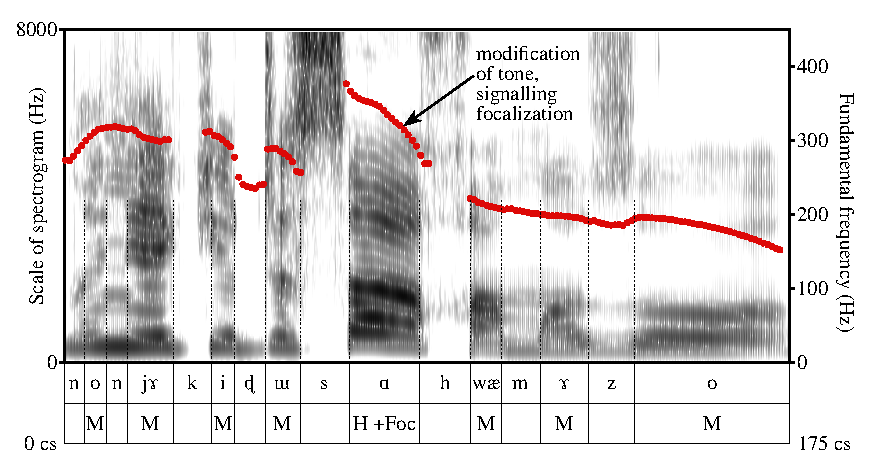
\includegraphics[width=\textwidth]{figures/F/F.eps}
	\caption{Spectrogram and F\textsubscript{0} curve for example (\ref{ex:nogift}), showing a~noticeable fall plus {lengthening} on the syllable /\ipa{sɑ˥}/ in /\ipa{ɖɯ˧-sɑ˥}/ ‘anything’. Top line of annotation: segments; bottom line: tones, with the added mention ‘+Foc’ for the syllable receiving intonational {focalization}.}
	\label{fig:noneedforbuying}
\end{figure}

This phenomenon is found in rapid speech as well as in slow repetitions.

It was later realized that the same type of prominence"=lending local intonational modification could
also be found for the two rising contours: high"=rising (MH) and low"=rising (LH). For these
contours, the modification consists of \isi{lengthening} and F\textsubscript{0} \isi{range expansion}. Due to the phonetic fact that these are phonological contours, which by themselves have
greater \isi{duration} than simple levels, the intonational modification is less salient perceptually than for the M
and H levels. Recognition of the existence of this phenomenon for the L level came last.

On the {analogy} of \ili{Naxi}, where a~reduced M- or L-tone syllable can result in the creation of
contours \citep{michaudetal2007d} which bear some phonetic similarity to those of Yongning Na, it was first hypothesized that there must be a~reduced
syllable in examples such as (\ref{ex:shedidnotgreetanyone}): $\ddagger${\kern2pt}\ipa{ɖɯ˧-kʰwɤ˥-ə˩
  mɤ˧-pi˥}. Likewise, example (\ref{ex:invitationtoeat}) was initially transcribed as $\ddagger${\kern2pt}\ipa{ə˧-dzɤ˧${\sim}$dzɤ˥-ə˩
  dzɯ˧}. Subsequent investigation showed that these notations were inappropriate. The dip in
fundamental frequency, accompanied by \isi{lengthening}, is
a~purely intonational device: it does not involve an added syllable.

%\Hack{\newpage}

\begin{exe}
	\ex
	\label{ex:invitationtoeat}
	\ipaex{ə˧-dzɤ˧${\sim}$dzɤ˥ F {\kern2pt}|{\kern2pt} dzɯ˧!}\\ 
	\gll ə˧-dzɤ˧${\sim}$dzɤ˥		F			 	dzɯ˥\\
	slowly		\textsc{focalization}		to\_eat\\
	\glt ‘Eat slowly!/Take your time!’ (Polite invitation to eat.)
\end{exe}

The realization of \isi{focalization} comprises a~movement in F\textsubscript{0}, a~slight \isi{lengthening}, and perhaps a~slight change in the vowel, as if a~final \textit{schwa} target were added after the vowel. This is sufficiently precise and specific to preserve tonal distinctions (avoiding headlong conflict with lexical tone). To put it differently, no \isi{neutralization} of lexical tonal contrasts takes place under \isi{focalization}. Emphatic tone is likewise
identifiable as such, from cues other than fundamental frequency. This limits the
possibility of a~\isi{misperception} of lexical tone caused by these intonational phenomena.


\subsubsection{Borderline cases}
\label{sec:borderlinecasesopeningintoadiscussionofthecategoricalstatusofthephenomenon}

About two hundred instances of intonational \isi{focalization} are indicated in the first twenty transcribed
texts. Some cases are clearer than others. For one thing, cases where this \isi{focalization} is
superimposed on rising contours, and on L tones, appear less salient for phonetic reasons, as outlined above. For another, there are borderline cases, where it is not obvious whether to add a~‘\ipa{F}’ in the
transcription or not. Borderline cases do not by themselves cast doubt on the categorical nature of the phenomenon. Intonational \isi{focalization} can be toned down, in the same way as \isi{emphatic stress} has toned"=down avatars shading into non"=emphatic realizations; this is a~common situation in the field of \isi{intonation}. On the other hand, it should be borne in mind, when consulting the texts, that the ‘\ipa{F}' and ‘\ipa{↑}' symbols (for intonational \isi{focalization} and \isi{emphatic stress}, respectively) cannot be assigned with the same degree of certainty as consonants, vowels and tones. For instance, the syllable /\ipa{li˩}/ ‘to see’ is transcribed in (\ref{ex:FLex})\footnote{In (\ref{ex:FLex}), the second and third syllables of /\ipa{ʈʂʰɯ˧ne˧-ʝi˥}/ ‘thus’ are coalescent, and fully undistinguishable on the spectrogram (\figref{fig:FL}). For convenience, a~simplified transcription as [\ipa{ʈʂʰɯ˧ne˧ gv̩˧˥}] is adopted in the surface phonological transcription of the sentence, and in the annotation to the spectrogram, in preference to /\ipa{ʈʂʰɯ˧ne˧-ʝi˧ gv̩˧˥}/. This case of coalescence is analyzed in Appendix A, \sectref{sec:smoothphoneticonsets}.} with an indication of intonational \isi{focalization}, on the basis of the auditory impression that it stands out in the flow of speech. The proposed translation for /\ipa{hĩ˧ li˩ F mɤ˩-ʁo˩}/ in (\ref{ex:FLex}) is ‘{\dots}~could not \textit{even} see people’, to reflect the pragmatic implications of focalization on the verb ‘to see’. The sequence /\ipa{hĩ˧ li˩ mɤ˩-ʁo˩}/, without intonational \isi{focalization}, would simply mean ‘{\dots}~could not see people’. 

\begin{exe}
	\ex
	\label{ex:FLex}
	\ipaex{le˧-mo˩, {\kern2pt}|{\kern2pt} le˧-mo˩, {\kern2pt}|{\kern2pt} njɤ˩ɭɯ˧ {\kern2pt}|{\kern2pt} ʈʂʰɯ˧ne˧ gv̩˧˥, {\kern2pt}|{\kern2pt} hĩ˧ li˩ F mɤ˩-ʁo˩!}\\ 
	\gll le˧-				mo˩\textsubscript{a}		njɤ˩ɭɯ˧		ʈʂʰɯ˧ne˧-ʝi˥		gv̩˧\textsubscript{c}				hĩ˥		 li˧\textsubscript{a}	F	mɤ˧-		ʁo˧\\
	\textsc{accomp}		old								eye				thus				to\_occur		person		to\_look\_at	\textsc{focalization}	\textsc{neg}		to\_be\_able\_to/to\_manage\\
	\glt ‘[The dog] got older and older; and so, its eyes could not even look at people anymore / it could not even see people anymore!’ (Dog2.80)
\end{exe}

But looking at the spectrogram in \figref{fig:FL}, it appears that the syllable /\ipa{li˩}/ ‘to see’ is not strikingly different from its neighbours in terms of either \isi{duration} or fundamental frequency. Average fundamental frequency over the vowel /\ipa{i}/ in /\ipa{li˩}/ is two semitones lower than over the vowel /\ipa{ĩ}/ in the preceding syllable, /\ipa{hĩ˧}/ (210~Hz vs.\ 237~Hz), a~phonetic difference that is in keeping with the phonological tones (M vs.\ L). The decrease in fundamental frequency between /\ipa{li˩}/ and the two L-tone syllables that follow can be interpreted as a~straightforward case of \textit{declination}, a~phenomenon mentioned in \sectref{sec:syntacticintonationphrasingandjunctures}.  

The data is nonetheless compatible with the hypothesis (based on auditory impression) that the syllable /\ipa{li˩}/ ‘to see’ is highlighted by intonational means. In terms of \isi{duration}, the syllable /\ipa{li˩}/ is 20~centiseconds long, which is slightly above the average for the passage shown in \figref{fig:FL} (100 centiseconds for seven syllables, i.e.\ about one syllable every 15 centiseconds). This difference in length cannot be dismissed as linked to the syllable's phonemes: if anything, the vowel /\ipa{i}/ would be expected to be intrinsically \textit{shorter} than other vowels \citep{dicristoetal1986, whalenetal1998}. As for fundamental frequency, the display in \figref{fig:FL}, covering the range from 0~Hz to 450~Hz, gives the impression of a~relatively smooth curve over the last four syllables, but if the scale is changed to a~narrower range, as in \figref{fig:FLCloseup}, the hump at the beginning of the vowel /\ipa{i}/ in /\ipa{li˩}/ becomes more salient visually. This hump, which results in a~dip of 2.5 semitones in the brief course of this vowel, could be significant: there is no obvious contextual reason why the hump should be present, therefore it makes sense to interpret it as one of the phonetic correlates of a~local intonational modification signalling some sort of emphasis, such as the phenomenon of intonational \isi{focalization} transcribed here as ‘\ipa{F}’.

\begin{figure}[ht]
	\includegraphics[width=\textwidth]{figures/FL/FL.eps}
	\caption{Spectrogram and F\textsubscript{0} curve for example (\ref{ex:FLex}), showing a~slight fall plus hints of {lengthening} on the syllable /\ipa{li˩}/ ‘to see’. Top line of annotation: segments; bottom line: tones, with the added mention ‘+Foc’ for the syllable presumed to receive intonational focalization.}
	\label{fig:FL}
\end{figure}

\begin{figure}[ht]
	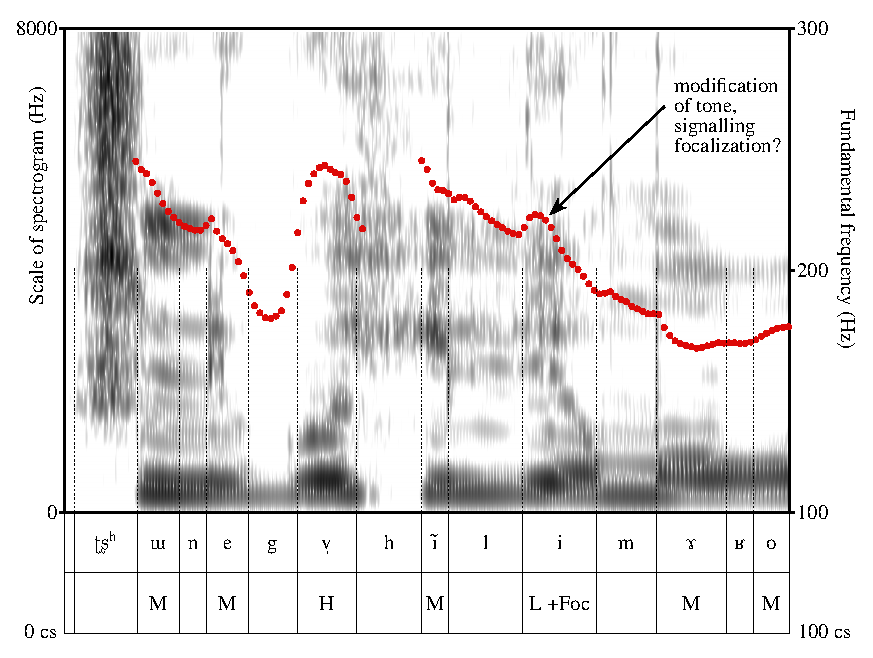
\includegraphics[width=\textwidth]{figures/FL/FLCloseup.eps}
	\caption{Same data as in \figref{fig:FL}, adopting a~narrower range for F\textsubscript{0} display.}
	\label{fig:FLCloseup}
\end{figure}

When transcribing narratives, one way to check with the speaker whether to classify a~given case as having intonational \isi{focalization} or not consists in playing the passage at issue, then repeating it with and without the telltale fall in pitch and \is{lengthening}lengthened rhyme, and asking the consultant to indicate which of the two realizations fits better. This entails no guarantee, however: even supposing that the investigator is successful in producing the intended distinction, the consultant may not base her decision on the realization heard on the recording. She may go for the realization which she considers (in retrospect) would have been more suitable in that context. 

Pending experimental verification by perceptual tests, it seems likely that different speakers have different degrees of sensitivity to intonational detail. Toned"=down versions of intonational \isi{focalization} may go unnoticed by some speakers. It is a~fact of life that hearers can fail to pick up intended clues. A~linguist's aphorism has it that, in human communication, misunderstanding is the general case, and mutual understanding is a~special case (``la compréhension est un cas parti\-culier du malentendu'': \citealt[39]{culioli1990}). The world is a~cemetery of cultures, and each text is a~tomb for allusions.\footnote{Lost allusions are often staged in literary works, among them Proust's \textit{In Search of Lost Time}. The grandmother's sisters design allusions that are so carefully veiled that they are unintelligible to the intended addressees: ``{\dots}~they, in their horror of vulgarity, had brought to such a~fine art the concealment of a~personal allusion in a~wealth of ingenious circumlocution, that it would often pass unnoticed even by the person to whom it was addressed.'' Scott Moncrieff translation revised by Terence Kilmartin. \textit{Original text:} ``Celles"=ci par horreur de la vulgarité poussaient si loin l’art de dissimuler sous des périphrases ingénieuses une allusion personnelle qu’elle passait souvent inaperçue de celui même à qui elle s’adressait.''} 

\subsubsection{A case in which intonational focalization has become habitual}
\label{sec:acaseofhabitualassociationofintonationalfocalizationtoaphraseillustratingtheaffinitiesbetweenfocalizationandnegation}

This paragraph presents a~case of habitual association of intonational \isi{focalization} to a~phrase. The classifier /\ipa{sɑ˥}/ ‘thing’ only appears in the phrase /\ipa{ɖɯ˧-sɑ˥}/ ‘anything’, itself
restricted to negative contexts: typical examples are shown in (\ref{ex:isntanything}) and (\ref{ex:donothing}).

\begin{exe}
	\ex
	\label{ex:isntanything}
	\ipaex{ɖɯ˧-sɑ˥ F {\kern2pt}|{\kern2pt} mɤ˧-dʑo˧.}\\ 
	\gll ɖɯ˧	sɑ˥		F	mɤ˧-	dʑo˧\textsubscript{b}\\
	one		\textsc{clf}.things		\textsc{focalization}	\textsc{neg}		to\_possess\\
	\glt ‘[I/they] don't have anything at all~/ [I/they] have nothing at all.’
\end{exe}

\begin{exe}
	\ex
	\label{ex:donothing}
	\ipaex{ɖɯ˧-sɑ˥ F {\kern2pt}|{\kern2pt}
		mɤ˧-ʝi˥}\\ 
	\gll ɖɯ˧	sɑ˥		F	mɤ˧-	ʝi˥\\
	one		\textsc{clf}.things		\textsc{focalization}	\textsc{neg}		to\_do\\
	\glt ‘to do nothing, to slob around the place, to do bugger all’
\end{exe}

Out of thirty examples of /\ipa{ɖɯ˧-sɑ˥}/ found in twenty"=five transcribed narratives, all but one are accompanied by intonational \isi{focalization}. The existence of one example without intonational \isi{focalization} (Trader\-AndHisSon.24) is enough to demonstrate that the association of this \isi{focalization} with /\ipa{ɖɯ˧-sɑ˥}/ is habitual, and should not be considered a~lexicalized characteristic of this expression in F4’s speech. 


\subsubsection{Intonational focalization and the division of the utterance into tone groups}
\label{sec:intonationalfocalizationandthedivisionoftheutteranceintotonegroups}


As discussed in Chapter~\ref{chap:toneassignmentrulesandthedivisionoftheutteranceintotonegroups}, the division of the utterance into tone groups is a~fundamental dimension
of Yongning Na \isi{prosody}. The sifting of examples reveals that intonational \isi{focalization} does not
necessarily entail the presence of a~following tone"=group \is{boundary (between tone groups)}boundary, as shown by (\ref{ex:hadtomarry}).


\begin{exe}
	\ex
	\label{ex:hadtomarry}
	\ipaex{ə˧ʝi˧-ʂɯ˥ʝi˩ {\kern2pt}|{\kern2pt} ɖɯ˩ɖʐɯ˧-ɬɑ˩tsʰo˩ ɳɯ˩ {\kern2pt}|{\kern2pt} ɖɯ˧-ʑi˩-ki˩ F ki˩-zo˩!}\\ 
	\gll ə˧ʝi˧-ʂɯ˥ʝi˩	ɖɯ˩ɖʐɯ˧-ɬɑ˩tsʰo˩	ɳɯ˧				ɖɯ˧-ʑi˩		-ki˧	F	ki˧\textsubscript{a}	-zo˧\textsubscript{a}\\
	long\_ago	{\textit{proper name}}		\textsc{a}		one-\textsc{clf}.households				\textsc{dat}	\textsc{focalization}	to\_give	\textsc{oblig}\\
	\glt ‘Long ago, Ddeezzhi Lhaco had to marry into someone's family!’ {\newline}(BuriedAlive3.143)
\end{exe}

In
the vast majority of examples, such a~\is{boundary (between tone groups)}boundary is present, however. Moreover, there are examples
where the intonational \isi{focalization} is associated to the insertion of a~tone"=group \is{boundary (between tone groups)}boundary at
a~place where it would otherwise be highly unexpected, as in (\ref{ex:boysmother}).

\begin{exe}
	\ex
	\label{ex:boysmother}
	\ipaex{zo˧ F {\kern2pt}|{\kern2pt} ə˧mi˧ ɳɯ˧ {\kern2pt}|{\kern2pt}mv̩˩-ki˥ ʐwɤ˩.}\\ 
	\gll zo˥		F							ə˧mi˧		ɳɯ˧	 				mv̩˩˥			-ki˧ 			ʐwɤ˩\textsubscript{b}\\
	son/man		\textsc{focalization}	mother	\textsc{a}	daughter/girl		\textsc{dat}	to\_speak\\
	\glt ‘The young man's mother talked to the young woman.’ (BuriedAlive3.161)
\end{exe}

The emphasis placed on /\ipa{zo˧}/ ‘son, man’ causes the insertion of  a~tone"=group \is{boundary (between tone groups)}boundary inside the phrase ‘the young man’s mother’. This results in a~different sequence of tones than is found in the phrase ‘the boy’s mother’, which, outside this context, is /\ipa{zo˧-ə˧mi˥}/. The division of this phrase into two tone groups results in the non"=application of the tone rules
which hold in determinative compounds, since tone rules never apply across tone"=group boundaries. 


\section[Intonational modifications as a~path towards the loss of lexical tone]{Habitual intonational modifications as a~path towards the loss of lexical tone}
\label{sec:expressiveandiconicphenomena}
\label{sec:towardsthelossoflexicaltoneonsomegrammaticalwordsthroughhabitualintonationalmodifications}

Expressive coinages and iconic phenomena constitute marginal elements: each of them has a~lilt of its own, and only bears loose links to the rest of the linguistic system. On the other hand, these phenomena undergo continuous attraction from the more central structures that make up the language's phonological system. There is thus a~tendency towards their integration into the language's phonological categories. Segmental examples are discussed in Appendix A (\sectref{sec:expressivecoinagesandmore}); the present section is devoted to an example that concerns tone. 

In Yongning Na, there are eight extra"=distal locative expressions, which share a~specific \isi{intonation}. The argument proposed here is that this habitual intonation constitutes a~path towards the loss of lexical tone on the grammatical morphemes at issue. These locative expressions are listed in \tabref{tab:expressivelocatives}, where their first syllable is transcribed with an exclamation mark ‘!’ instead of a~tone mark, as a~provisional device to represent their telltale \isi{intonation}. 

\begin{table}%[t]
	\caption{Extra"=distal locative expressions carrying specific {intonation}.}
	\begin{tabularx}{\textwidth}{ l Q l@{\hspace{10mm}} l }
		\lsptoprule
		locative & meaning & 1\textsuperscript{st} σ & meaning of 1\textsuperscript{st} σ\\\midrule
		\ipa{gɤ!-qo˧} & way up & \ipa{gɤ˩-} & upward\\
		\ipa{gɤ!-ʈʂʰɯ˧qo˧} & way up there (\textsc{prox}) & \ipa{gɤ˩-} & upward\\
		\ipa{gɤ!-tʰv̩˧qo˧} & way up there (\textsc{dist}) & \ipa{gɤ˩-} & upward\\
		\ipa{gɤ!-tʰv̩˧-gi\#˥} & way up in that direction & \ipa{gɤ˩-} & upward\\ \addlinespace \hdashline \addlinespace
		\ipa{dɤ!-qo˧} & way over there & ? & ?\\
		\ipa{dɤ!-ʈʂʰɯ˧qo˧} & way over there (\textsc{prox}) & ? & ?\\
		\ipa{dɤ!-tʰv̩˧qo˧} & way over there (\textsc{dist}) & ? & ?\\
		\ipa{dɤ!-tʰv̩˧-gi\#˥} & way over in that direction & ? & ?\\
		\lspbottomrule
	\end{tabularx}
	\label{tab:expressivelocatives}
\end{table}

The two sets of extra"=distal locatives shown in \tabref{tab:expressivelocatives} are parallel in terms of their syntactic composition, and they share the same \isi{intonation}. The realization of their first syllable is highly expressive and allows
variants. Either it starts on an~extra"=high pitch and glides downward, at a~slope left to the
speaker’s discretion: a~sharp fall or a~prolonged one. Or it is rising, the details of the rise
(\isi{duration}, slope and peak height) being again left to the speaker’s discretion. As far as could be
ascertained, the sharply falling \is{variants}variant emphasizes the great distance to the place at issue
(paraphrase: ‘in a~place far, far away’), whereas the rising \is{variants}variant (exemplified in \figref{fig:distalrising}) is used to direct the listener’s
attention to that place, against a~background of shared knowledge (paraphrase: ‘that faraway
place, you know’). For instance, the context for (\ref{ex:yourdaughteriswayoverthere}) is the following: a~mother thinks that her daughter has died; the young woman's lover tells the mother that her daughter is still alive, and that she is in hiding. The young man knows where the young woman is, but does not wish to disclose it to the mother. The extra"=distal locative in (\ref{ex:yourdaughteriswayoverthere}) does not emphasize the great distance: paraphrase as ‘Your daughter is in a~faraway place’ would be inappropriate. In this context, the syllable /\ipa{dɤ}/ in \ipa{dɤ!-tʰv̩˧qo˧}/ ‘way over there’ is realized as rising: see the fundamental frequency tracing in \figref{fig:distalrising}.

\begin{exe}
	\ex
	\label{ex:yourdaughteriswayoverthere}
	\ipaex{no˧ mv̩˩  {\kern2pt}|{\kern2pt} dɤ!-tʰv̩˧qo˧ dʑo˩.}\\ 
	\gll no˩	mv̩˩˥		dɤ!-tʰv̩˧qo˧	dʑo˩\textsubscript{b}\\
	\textsc{2sg}	daughter	\textsc{dem.extra\_distal}		\textsc{exist}.animated\_beings\\
	\glt ‘Your daughter is [in a~place that I know,] way over there.’ {\newline}(BuriedAlive3.105)
\end{exe}

\begin{figure}[ht]
	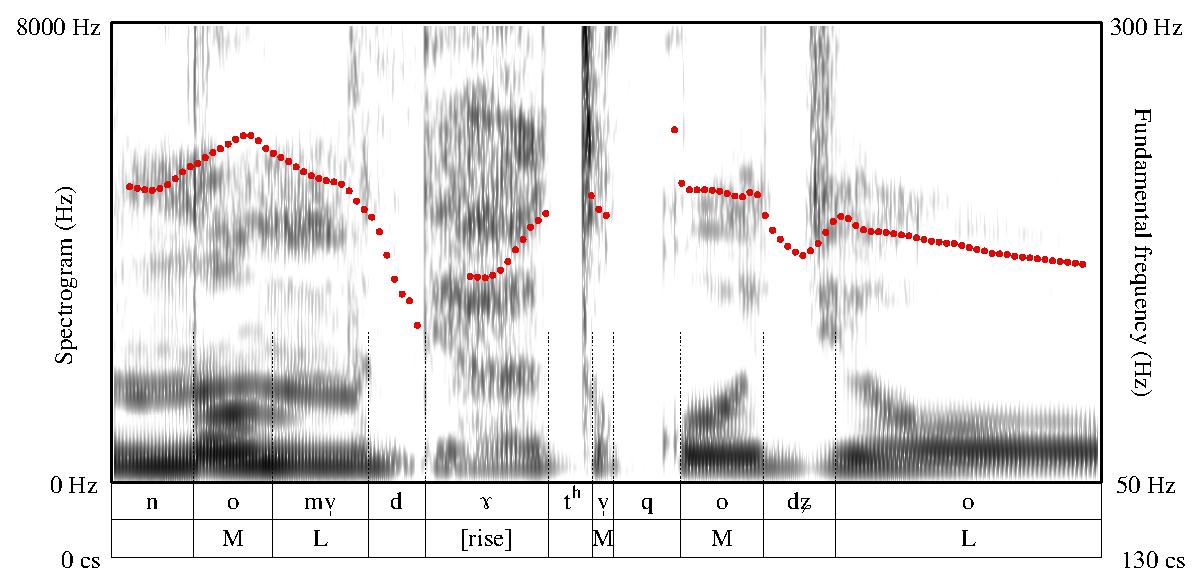
\includegraphics[width=\textwidth]{figures/Xdistal/distal.eps}
	\caption{Spectrogram and F\textsubscript{0} curve for example (\ref{ex:yourdaughteriswayoverthere}), showing the rising realization of the syllable /\ipa{dɤ}/ in /\ipa{dɤ!-tʰv̩˧qo˧}/ ‘way over there’.}
	\label{fig:distalrising}
\end{figure}

Use of tone marks to stylize the perceived pitch of the syllable /\ipa{dɤ}/ in these locative expressions, such as
/\ipa{dɤ˥˩}/ for a~fall from top to bottom of the pitch range, /\ipa{dɤ˧˥˥}/ for a~rise followed by a~plateau, or /\ipa{dɤ˧˥}/ for a~rise from mid"=range to top of pitch range, would introduce a~potential for confusion between lexical tone and
intonational phenomena. Devising a~set of symbols for more detailed transcription would
require a~full"=fledged study of expressive phenomena in Yongning Na; this falls outside the scope of this exploratory chapter.

Identification of the \is{prefixes}prefix /\ipa{gɤ˩-}/ ‘upward’ in the locative expressions /\ipa{gɤ˩-qo˧}/, /\ipa{gɤ˩-ʈʂʰɯ˧qo˧}/, /\ipa{gɤ˩-tʰv̩˧qo˧}/ and
/\ipa{gɤ˩-tʰv̩˧-gi\#˥}/ of \tabref{tab:expressivelocatives} is not problematic, as this \is{prefixes}prefix is attested elsewhere in the language, in a~number of productive constructions, with the same meaning that it has in the extra"=distal
locatives (see \sectref{sec:themarkingofspatialorientationonverbs}). On the other hand, it is an~issue how to analyze the extra"=distal
locatives /\ipa{dɤ!-qo˧}/, /\ipa{dɤ!-ʈʂʰɯ˧qo˧}/, /\ipa{dɤ!-tʰv̩˧qo˧}/ and
/\ipa{dɤ!-tʰv̩˧-gi\#˥}/, because the syllable /\ipa{dɤ}/ is synchronically orphaned. It is peculiar not only in its intonational
realization, but also in its segmental composition. Apart from extra"=distal locative expressions, this combination of initial and rhyme is only attested in Yongning Na in /\ipa{hṽ̩˧dɤ˧ɻ̍\#˥}/
‘clumsy’ and /\ipa{õ˧dɤ˧ɻ̍˧}/ ‘fundamental(ly)’. In both of these words, the syllable /\ipa{dɤ}/ is followed by /\ipa{ɻ}{\kern2pt}/; since rhotic sounds are known (cross"=linguistically) to have especially strong {coarticulatory} effects (see for instance \citealt{west1999}), it is far from implausible that the combination /\ipa{dɤ}/ in these two words results from the phonologization of phonetic {coarticulation}. 

My best guess at the time of writing is that the syllable /\ipa{dɤ}/ in extra"=distal
locatives originates in an expressive deformation of the extra"=distal morpheme //\ipa{dv̩˩}//. This morpheme appears in /\ipa{dv̩˩-tɕo˧}/ ‘that way, that direction’, an expression now almost fallen into disuse which is structurally parallel to /\ipa{ʈʂʰɯ˧-tɕo˧}/ ‘this way’ and /\ipa{tʰv̩˧-tɕo˧}/ ‘that way’. The expression /\ipa{dv̩˩-tɕo˧}/ alone is not enough to determine the tone of the extra"=distal morpheme //\ipa{dv̩}// with certainty: it is necessary to observe a~morpheme in several contexts of occurrence in order to arrive at its lexical tone, as explained step by step in the discussion of the lexical tones of nouns in Chapter~\ref{chap:thelexicaltonesofnouns}, and verified in the discussion of grammatical words in Chapters~\ref{chap:combinationsofnounswithgrammaticalwords}--\ref{chap:verbsandtheircombinatoryproperties}. But the presence of a~L tone on the first syllable in /\ipa{dv̩˩-tɕo˧}/ ‘that way, that direction’ suggests that the tone of the extra"=distal morpheme
/\ipa{dv̩}/ is likely to be L or LM, hence the provisional adoption of an internal \is{comparative method (historical linguistics)}reconstruction as *\ipa{dv̩˩}.

From a~synchronic point of view, however, there is no evidence for positing an~initial lexical L tone in the extra"=distal locatives /\ipa{dɤ!-qo˧}/,
/\ipa{dɤ!-ʈʂʰɯ˧qo˧}/, /\ipa{dɤ!-tʰv̩˧qo˧}/ and /\ipa{dɤ!-tʰv̩˧-gi\#˥}/. This set has the same prosodic realization as the set consisting of /\ipa{gɤ!-qo˧}/, /\ipa{gɤ!-ʈʂʰɯ˧qo˧}/, /\ipa{gɤ!-tʰv̩˧qo˧}/, and /\ipa{gɤ!-tʰv̩˧-gi\#˥}/ (shown in \tabref{tab:expressivelocatives}), but this realization is
so distant from what one would expect on the basis of the lexical L tone of /\ipa{gɤ˩-}/ ‘upward’
that it looks like a~case of \isi{neutralization} of all tonal oppositions on the first syllable of these
locatives.  

While the synchronic data provides no evidence for one tonal notation rather than another, it also provides no evidence against adopting a~notation of /\ipa{dɤ-}/ with L tone, as suggested by language"=internal evidence. Therefore, notation as /\ipa{dɤ˩-}/ is provisionally adopted, rewriting \tabref{tab:expressivelocatives} as \tabref{tab:expressivelocativesUNDER}. 

\begin{table}%[t]
	\caption{Extra"=distal locative expressions carrying specific {intonation}.}
	\begin{tabularx}{\textwidth}{ l Q l@{\hspace{10mm}} l }
		\lsptoprule
		locative & meaning & 1\textsuperscript{st} σ & meaning of 1\textsuperscript{st} σ\\\midrule
		\ipa{gɤ˩-qo˧} & way up & \ipa{gɤ˩-} & upward\\
		\ipa{gɤ˩-ʈʂʰɯ˧qo˧} & way up there (\textsc{prox}) & \ipa{gɤ˩-} & upward\\
		\ipa{gɤ˩-tʰv̩˧qo˧} & way up there (\textsc{dist}) & \ipa{gɤ˩-} & upward\\
		\ipa{gɤ˩-tʰv̩˧-gi\#˥} & way up in that direction & \ipa{gɤ˩-} & upward\\ \addlinespace \hdashline \addlinespace
		\ipa{dɤ˩-qo˧} & way over there & *\ipa{dv̩˩-} & *\textsc{dem.dist}\\
		\ipa{dɤ˩-ʈʂʰɯ˧qo˧} & way over there (\textsc{prox}) & *\ipa{dv̩˩-} & *\textsc{dem.dist}\\
		\ipa{dɤ˩-tʰv̩˧qo˧} & way over there (\textsc{dist}) & *\ipa{dv̩˩-} & *\textsc{dem.dist}\\
		\ipa{dɤ˩-tʰv̩˧-gi\#˥} & way over in that direction & *\ipa{dv̩˩-} & *\textsc{dem.dist}\\
		\lspbottomrule
	\end{tabularx}
	\label{tab:expressivelocativesUNDER}
\end{table}

The considerable intonational modification of the initial syllable in these locative expressions is
transcribed in narratives through the addition of the mark for \isi{emphatic stress} ‘\ipa{↑}’ (see \sectref{sec:emphaticstressanditstoneddownavatars}). This mark does not
tell the full story, but has the advantage of bringing attention to the presence of a~strong
intonational modification resulting in a~gap between the hypothesized lexical tone and the phonetic realization. Such unstable situations hold special potential for reinterpretation and change.

\section{Key factors in the phonetic implementation of tone}
\label{sec:keyfactorsinthephoneticimplementationoftone}

This section sets out what I believe to be key factors in the phonetic implementation of tone in Yongning Na.

\subsection{Intonational backgrounding of function words}
\label{sec:consequencesoftheweakrealizationofgrammaticalwords}
\label{sec:intonationalbackgroundingofparticles}

It is a~well"=established cross"=linguistic observation that grammatical words are less strongly
articulated than lexical words: 
the lighter semantic weight of grammatical
words relative to lexical words is reflected in a~weaker phonetic realization. In languages that have distinctive stress, many grammatical words do
not carry lexical stress, and those that do are sometimes destressed in discourse; in some languages
that have tone, there are cases of toneless grammatical words, for instance in \ili{Mandarin} \citep{linetal1980,chenetal2006}. Even in languages where there is no phonological difference between lexical words and
grammatical words (e.g.~in \ili{French}, which does not have lexical stress, and in \ili{Vietnamese}, which
has tone on all syllables including grammatical morphemes), the phonetic difference between these
two categories is noticeable. The extent of the difference in strength of articulation varies across languages: it has been found that there was less hypo"=articulation of
grammatical words in \ili{Vietnamese} than in \ili{English} or \ili{French} \citep{brunelle2015}.  

Africanist colleagues report that the
phonetic realization of tone sequences in some Subsaharan languages is unaffected (or almost
unaffected) by the nature of the syllables that act as tone"=bearing units, so that a~M tone on
a~grammatical morpheme will be realized in the same way as if the tone"=bearing syllable were a~verb
or a~noun (Jacqueline Leroy, p.c.\ 2007 and Larry Hyman, p.c.\ 2011). In Yongning Na, on the other hand, the intonational
backgrounding of grammatical words such as sentence"=final particles is easily noticed. 

The {prohibitive} \is{prefixes}prefix /\ipa{tʰɑ˧-}/ is a~case in point. When it is followed by a~reduplicated verb
of tone category M\textsubscript{a}, the tone pattern is M.H.L,
e.g.~/\ipa{tʰɑ˧-ki˥}${\sim}$\ipa{ki˩}/ ‘do not give away, do not distribute’. Phonetically, the
syllable /\ipa{tʰɑ˧}/ is realized with rising fundamental frequency. Averaging across the eight tokens in the recording VerbProhib,
there is a~6.7\% rise in F\textsubscript{0} (standard deviation: 3.6). This
rise is probably too small to be perceived as such: glissandos need a~minimum slope of about 14\%
over a~long tone"=bearing unit (over 300 ms) or 18\% over a~short tone"=bearing unit (100 ms)
\citep{rossi1971b,gsell1979b}. The amplitude of the rise during /\ipa{tʰɑ˧-}/ can be compared with
the 16\% jump in F\textsubscript{0} (standard deviation: 5.0) from the
\is{prefixes}prefix to the H-tone syllable that follows. To use a~concept
proposed as part of a~model for {Mandarin} speech synthesis, grammatical words could be said to have a~lower \textit{strength
coefficient}. In this model (called Stem"=ML, for \textit{Soft Template Mark-up Language}), the tones of syllables with a~high strength coefficient are
realized close to their lexical tone template, whereas the lower the coefficient, the stronger the
\isi{coarticulation} with following tones \citep{kochanskietal2003b}. The anticipatory rise in the course of the {prohibitive} \is{prefixes}prefix /\ipa{tʰɑ˧-}/ can be interpreted as a~typical example
of \isi{coarticulation} between a~M-tone syllable with low strength coefficient and a~following H-tone
syllable with high strength coefficient.

For future studies of this topic, direct phonetic comparison would be possible between segmentally and tonally \is{homophony}homophonous pairs such as the noun /\ipa{bv̩˧}/ ‘intestine’ and the \isi{possessive} /\ipa{=bv̩˧}/, and the noun for
‘person, human being’, \mbox{/\ipa{hĩ˥}/}, and its grammaticalized avatar as a~{relativizer}, \mbox{/\ipa{-hĩ˥}/}.


\subsection{The absence of oppositions between /L.M/ and /L.H/, or between /H.M/ and /H.L/}
\label{sec:theabsenceofoppositionsbetweenlmandlhorbetweenhmandhl}

Two of the key phonological facts about Yongning Na tone are (i)~that there is no contrast between /H.M/ and /H.L/
sequences (only /H.L/ is observed), and (ii)~that the contrast between \mbox{//LM//} and \mbox{//LH//}, which is postulated at
the \is{form!underlying}underlying phonological level, is neutralized in \is{form!surface}surface phonological forms. This leads to
the following generalization: in Yongning Na surface phonological tone sequences, there is no context where a~two"=step shift on the
tone scale (i.e.\ from /L/ to /H/, or from /H/ to /L/) contrasts with a~one"=step shift (i.e.\ from /L/ to /M/, or
from /H/ to /M/). This is unlike the closely related language \ili{Naxi}, where all combinations of tones in disyllables
are attested, including /L.H/, /L.M/, /H.M/ and /H.L/.

This state of affairs has important consequences for the production and perception of tone sequences. For any pair of successive syllables within a~\isi{tone group}, it is enough to identify
the tone of the second as being (i)~higher than the preceding tone, (ii)~on the same level as the preceding
tone, or (iii)~lower than the preceding tone.


\subsection[Anticipatory dissimilation in M.L and M.H sequences]{Anticipatory phonetic dissimilation in M.L and M.H sequences}
\label{sec:tonalcoarticulationanticipatoryphoneticdissimilationinmlandmhsequences}

In some Subsaharan languages, phonetic anticipation of following tones takes place: in a~L.L.H sequence, the
second L tone is realized higher than the first, in a~gradual progression towards the H
tone \citep[216]{creissels1994}. Auditory impression suggests that the opposite happens in Yongning Na. If a~M tone is followed by L, this M tone is
realized with a~higher fundamental frequency than when followed by H. This has the effect of
bringing out the contrast in pitch between M and the following tone. The M tone can be said to have
three allotones: that found in front of L is the highest; that found in front of M or MH is in a~central
phonetic range of F\textsubscript{0}; and that found in front of H is the
lowest.

Likewise, a~L tone is realized lower in front of M or H than when followed by another L. Using the
vertical position of letters to indicate relative pitch, an~approximation of the phonetic
realization of a~M.M.L sequence would be [M.\raisebox{0.3ex}{M}.\raisebox{-0.3ex}{L}], and a~L.L.H sequence could be approximated as
[L.\raisebox{-0.3ex}{L}.\raisebox{0.4ex}{H}].

These \is{coarticulation|textbf}coarticulatory phenomena link up with observations about the realization of like"=tone sequences, L.L.L... and
M.M.M... (H.H.H... sequences are never observed, since a~H tone is always followed by L: this is formulated in \sectref{sec:alistoftonerules} as Rule~4, “The syllable following a~H-tone syllable receives L tone”). Sequences
of L tones decline gradually towards a~final L target that is clearly low. The first L tone in such
a~sequence may be realized in a~relatively high range of fundamental frequency: extracted from
context, it may sound like [M]. This does not threaten its correct identification within the tone
sequence: a~sequence such as L.L.L cannot be mistaken for M.M.L, because the latter sequence has to
be realized with a~significant phonetic drop from M to L (approximation:  [M.\raisebox{0.3ex}{M}.\raisebox{-0.3ex}{L}]). In the absence of
the slight upward jump in fundamental frequency found from the first to the second M level in [M.\raisebox{0.3ex}{M}.\raisebox{-0.3ex}{L}], and of any sudden drop from one syllable to the
next, a~sequence of syllables realized with gradually decreasing fundamental frequency is perceived as consisting of like tones. Likewise, a~M.M.M like"=tone sequence
cannot be mistaken for M.M.L even if its last tone is depressed by intonational factors such as
final lowering. Final lowering affects the last syllable, but does not raise the previous one
(schematic representation: [M.M.\raisebox{-0.3ex}{M}]), whereas a~M.M.L sequence would comprise a~raising
of the syllable before last: [M.\raisebox{0.2ex}{M}.\raisebox{-0.3ex}{L}].

These auditory impressions are summarized in \tabref{tab:aschematicrepresentationoftherealizationofsometonesequencesinyongningna}. (Remember that the symbol σ is used to stand for syllables.) They receive some support from acoustic measurements reported in a~phonetic pilot study by a~speaker of Yongning Na \citep{a2016}; the logical next step would consist in conducting a~state"=of"=the"=art experimental study. 
%Of course, it should be kept in mind that this simplified description of the perception process is mostly based on auditory impressions in a~specific situation: that of a~non"=proficient speaker (namely the investigator) focusing on tone recognition. In communication among Na speakers, tone recognition is only a~small component within a~global interpretation process. 

\begin{table}%[t]
	\caption{\label{tab:aschematicrepresentationoftherealizationofsometonesequencesinyongningna}A schematic representation of the realization of some tone sequences in Yongning Na.}
{\renewcommand{\arraystretch}{1.35}	
\begin{tabularx}{\textwidth}{ P{18mm} l Q }
		\lsptoprule
		phonetic outline & interpretation & cues to tonal identification\\\midrule
		{[\raisebox{0.3ex}{σ}.\raisebox{0.2ex}{σ}.\raisebox{0.1ex}{σ}.σ.\raisebox{-0.3ex}{σ}]} & [\raisebox{0.3ex}{M}.\raisebox{0.2ex}{M}.\raisebox{0.1ex}{M}.M.\raisebox{-0.3ex}{M}] & gentle decline in F\textsubscript{0}; overall mid range of F\textsubscript{0}; final lowering is not considerable\\
		{[\raisebox{0.1ex}{σ}.\raisebox{0ex}{σ}.\raisebox{-0.1ex}{σ}.\raisebox{-0.3ex}{σ}.\raisebox{-0.5ex}{σ}]} & {[\raisebox{0.1ex}{L}.\raisebox{0ex}{L}.\raisebox{-0.1ex}{L}.\raisebox{-0.3ex}{L}.\raisebox{-0.5ex}{L}]} & slightly steeper decline in F\textsubscript{0} than for all-M sequences; slightly lower starting"=point and endpoint\\
		{[σ.σ.\raisebox{0.2ex}{σ}.\raisebox{-0.3ex}{σ}]} & M.M.\raisebox{0.2ex}{M}.\raisebox{-0.3ex}{L} & raising of the syllable before last, and clear difference in pitch between the last two syllables\\
		{[σ.\raisebox{-0.1ex}{σ}.\raisebox{-0.3ex}{σ}.\raisebox{0.4ex}{σ}]} & L.\raisebox{-0.1ex}{L}.\raisebox{-0.3ex}{L}.\raisebox{0.4ex}{H} & lowering of the syllable before last, and clear difference in pitch between the
		last two syllables\\
		\lspbottomrule
	\end{tabularx}}
\end{table}

Grasping the phenomenon of anticipatory phonetic \isi{dissimilation} in M.L and M.H sequences is crucial
to the identification of tones in Yongning Na. The system allows for a~great range of phonetic
\isi{variation} in sequences of L tones or M tones, since L-tone sequences may start from a~relatively high
pitch, as long as they descend clearly towards a~phonetic low target without intervening upward
jumps in pitch. M-tone sequences may be strongly affected by \isi{declination} (a phonetic, gradual,
noncategorical decrease in fundamental frequency in the course of the
utterance: see
\sectref{sec:syntacticintonationphrasingandjunctures})
without putting their identification at risk. Listeners confronted with a~sequence of syllables of
decreasing fundamental frequency, without noticeable upward jumps, can
safely interpret the sequence as carrying M.M.M... or L.L.L... tones; among these two possibilities, the overall slope of the
decrease in F\textsubscript{0}, and the range of F\textsubscript{0} reached at
the end of the sequence, guide the listener towards interpretation as either M.M.M... or L.L.L...

Anticipatory phonetic \isi{dissimilation} in M.L and M.H sequences is especially salient, but
preplanning in tone production is also noticeable at the level of the entire \isi{tone group}. For
instance, a~M.M.H sequence begins on a~lower pitch than M.M.M, which itself begins lower than M.M.L. A~striking example was
unintentionally recorded by eliciting verbs in frame (\ref{ex:framegoingto}).

\begin{exe}
	\ex
	\label{ex:framegoingto}
	\ipaex{no˧ ɳɯ˧ {\kern2pt}|{\kern2pt} V-zo˧-ho˩.}\\ 
	\gll no˩	ɳɯ˧	V	-zo˧\textsubscript{a}	-ho˩\\
	\textsc{2sg}		\textsc{a}	V	\textsc{oblig}	\textsc{fut}\\
	\glt ‘you must now V~/ you will now have to V.’
\end{exe}

The sequence ‘you will now have to eat’, /\ipa{no˧ ɳɯ˧} {\kern2pt}|{\kern2pt}
\ipa{dzɯ˧-zo˧-ho˥}/, was realized with high pitch on the two M-tone syllables of the
utterance"=initial \isi{tone group}, /\ipa{no˧ ɳɯ˧}/ (2\textsc{sg} plus \textsc{a}), whereas the two next M-tone syllables,
/\ipa{dzɯ˧-zo˧}/, were realized lower than average so as to maximize the contrast with the H tone
that follows them. The result is a~considerable drop in F\textsubscript{0}
from /\ipa{ɳɯ˧}/ to /\ipa{dzɯ˧}/, despite their identical phonological tone. Likewise, in the
elicited sentence (\ref{ex:horsestomach}), the M tones of /\ipa{hu˧mi˧}/ ‘stomach’ are realized
distinctly lower than those of /\ipa{ʐwæ˧zo˧=bv̩˧}/ ‘of \mbox{(a/the)} horse’.

\begin{exe}
	\ex
	\label{ex:horsestomach}
	\ipaex{ʈʂʰɯ˧ {\kern2pt}|{\kern2pt} ʐwæ˧zo˧=bv̩˧ {\kern2pt}|{\kern2pt} hu˧mi˧ ɲi˥.}\\ 
	\gll ʈʂʰɯ˥		ʐwæ˧zo\#˥	=bv̩˧	hu˧mi˥\$	ɲi˩\\
	\textsc{dem.prox}	colt	\textsc{poss}		stomach		\textsc{cop}\\
	\glt ‘This is the stomach
	of a~colt.’ (BodyPartsOfAnimals7.140)
\end{exe}

Similar evidence comes from narratives. In (\ref{ex:Funeral2016}), /\ipa{ɖɯ˧-ʁæ˩bæ˩}/ ‘one plateful’ was initially transcribed as $\ddagger${\kern2pt}\ipa{ɖɯ˧-ʁæ˧bæ˩}: due to final lowering, there is a~phonetic drop in F\textsubscript{0} from the second syllable (/\ipa{ʁæ˩}/) to the last syllable (/\ipa{bæ˩}/), even though these two syllables carry the same tone (L). This phonetic drop may be as
salient (or even more salient) than that from the first syllable (/\ipa{ɖɯ˧}/) to the second syllable (/\ipa{ʁæ˩}/), which carry different tones (M and L, respectively).
%the sequence /\ipa{ʁæ˧bæ˧-qo˧-ɳɯ˩}/ was
%initially transcribed $\ddagger${\kern2pt}\ipa{ʁæ˧bæ˧-qo˥-ɳɯ˩}, misinterpreting the phonetic raising of the M tone in
%front of L as a~phonological difference from the preceding two M tones. 

\begin{exe}
	\ex
	\label{ex:Funeral2016}
	\ipaex{ʁæ˧bæ˧-qo˧ ɳɯ˧ {\kern2pt}|{\kern2pt} ʁæ˧bæ˧ {\kern2pt}|{\kern2pt} ɖɯ˧-ɭɯ˧-qo˧ ɳɯ˧, {\kern2pt}|{\kern2pt} ɖɯ˧-ʁæ˩bæ˩!}\\ 
	\gll ʁæ˧bæ˧		-qo˧	ɳɯ˧		ʁæ˧bæ˧	ɖɯ˧	ɭɯ˧\textsubscript{b}	-qo˧	ɳɯ˧		ɖɯ˧		ʁæ˩bæ˩\\
	wooden\_plate	inside	\textsc{abl/top}	wooden\_plate	one	\textsc{clf}		inside	\textsc{abl/top}	one		\textsc{clf}.platefuls\\
	\glt ‘[The sweets used to be presented] on a~plate! [They were placed] on a plate; [one used to prepare] a plateful!’ (Funeral.216)
\end{exe}

This example brings us to the topic of the resetting of reference values for tones at junctures
between tone groups.


\subsection[Resetting of reference values at junctures between tone groups]{Resetting of reference values for tones at junctures between tone groups}
\label{sec:resettingofreferencevaluesfortonesatjuncturesbetweentonegroups}

As noted in \sectref{sec:syntacticintonationphrasingandjunctures}, 
a~phonetic, gradual, noncategorical decrease in fundamental frequency takes place in the course of the sentence. This is known as ‘\isi{declination}’. Fundamental frequency therefore fluctuates within a~gradually narrowed
range. Resetting of F\textsubscript{0} does not take place at each \is{boundary (between tone groups)}boundary between two tone groups. On the other
hand, there is a~\textit{resetting of reference values for tones} at each \is{boundary (between tone groups)}boundary between tone groups, such
that a~M tone in final position within a~\isi{tone group} and another M tone in initial position within
the following \isi{tone group} can have widely different fundamental frequency values. This also relates
to phonological facts on possible tonal contrasts in initial, medial and final position inside a~tone group: a~M tone in initial position within a~\isi{tone group} only contrasts with L, so that it has greater freedom of phonetic \isi{variation} than a~M tone in final position, where contrasts are more numerous. Remember that, after a~penultimate M tone, a~\isi{tone group} can end in any of L, M, H, MH or LH; this places precise constraints on a~final M tone's position within the tonal space. 
%(Monosyllabic tone groups constitute a~special case, where there are three tonal possibilities at the surface phonological level: M, LH, and MH.)


\subsection{The realization of rising contours}
\label{sec:therealizationoflmlhandmhcontours}


It was pointed out in Chapter~\ref{chap:thelexicaltonesofnouns} that there only exist two types of contours on monosyllables at the
surface phonological level: low"=rising and mid"=rising. At the \is{form!surface}surface phonological level, there is
no opposition between LM and LH contours. Phonologically, the product of the \isi{neutralization} is
labelled LH, for the structural reason set out in \sectref{sec:neutralizationoflmandlhinisolationistheproductlmorlh}. Phonetically, it is a~low"=rising {contour}
whose endpoint is not as high as that of the MH {contour}. To approximate phonetic realizations in
terms of three levels, they are closer to [LM] than to [LH]. This makes sense both in terms of
production and in terms of perception. In production, reaching as high a~phonetic target for the
low"=rising {contour} as for the mid"=rising {contour} would require extra effort, as the rise in
F\textsubscript{0} would have to be greater. In perception, this rise to
a~final target similar to that of the MH \is{tonal contour}contour could make it more difficult to distinguish the
(phonologically contrastive) low"=rising and mid"=rising contours. There are thus phonetic reasons why
the product of the \isi{neutralization} of LM and LH should be phonetically closer to [LM] than to
[LH].

From the point of view of the tone system, this creates a~tension between phonological categories
and phonetic realizations. Such discrepancies hold potential for reanalysis of the system by language learners, especially in the
present social context, where exposure to Na is made more limited by the pervasive presence of
{Mandarin}, so that children do not acquire the tonal system in its full richness. This issue
will be taken up in Chapter~\ref{chap:yongningnatonesinadynamicsynchronicperspective}.


\section{By way of recapitulation: Examples of mistaken tonal identification}
\label{sec:examplesofmistakeninterpretationsoftonalsequencesforwantoftakingtoneimplementationrulesintoaccount}

In this section, the observations made above about \isi{intonation} and tone implementation are recapitulated through examples of \is{mistakes}mistaken notations from early field notes: cases where tone identification was erroneous because the investigator was unaware of the language"=specific factors that go to shape the final prosodic form of utterances. These examples are intended to shed light on the process of
categorical interpretation of the pitch of successive syllables. 


\subsection{Anticipatory dissimilation before a~L tone}
\label{sec:anticipatorydissimilationbeforealtone}

The tone sequence M.M.L was often mistakenly transcribed as M.H.L, for instance in the determinative
\is{compounds}compound ‘tiger’s ear’, shown in (\ref{ex:tigerear}).

\begin{exe}
	\ex
	\label{ex:tigerear}
	\ipaex{lɑ˧-ɬi˧pi˩}\\ 
	\gll lɑ˧	ɬi˧pi˩\\
	tiger		ear\\
	\glt ‘tiger's ear’ (DetermCompounds6.17)
\end{exe}

This \is{compounds}compound was initially transcribed as $\ddagger${\kern2pt}\ipa{lɑ˧-ɬi˥pi˩}. This was
because the pitch of the second syllable, /\ipa{ɬi˧}/, is higher than that of the first, /\ipa{lɑ˧}/, due to anticipatory
\isi{dissimilation} before a~L tone, as described in \sectref{sec:tonalcoarticulationanticipatoryphoneticdissimilationinmlandmhsequences}: the successive pitch levels can be stylized as [M.\raisebox{0.3ex}{M}.\raisebox{-0.3ex}{L}]. The
difference in pitch between the first two syllables is a~cue to the M.L sequence that follows: this difference is important to the identification of the tone
of the third syllable as L, and not as a~M tone lowered by \textit{\isi{declination}} or \textit{\isi{final lowering}}. But it
must be factored out when determining the tone of the second syllable, /\ipa{ɬi˧}/.


\subsection{Interplay between morphosyntax and phonology}
\label{sec:theinterplaybetweenmorphosyntacticinformationandphonologicalinformationinspeechcomprehension}

The tone sequence M.L.L.L in (\ref{ex:forgotten}) was mistakenly transcribed as $\ddagger${\kern2pt}MH.M.L.L ($\ddagger${\kern2pt}\ipa{le˧˥-mv̩˧pʰæ˩-ze˩}) on my first field trip. 

\begin{exe}
	\ex
	\label{ex:forgotten}
	\ipaex{le˧-mv̩˩pʰæ˩-ze˩}\\
	\gll le˧-	mv̩˩pʰæ˧˥	-ze˧\textsubscript{b}\\
	\textsc{accomp}		to\_forget		\textsc{pfv}\\
	\glt ‘[I/you{\dots}] have forgotten’ (Source: field notes. Also found in Dog.4)
\end{exe}

Transcription as $\ddagger${\kern2pt}MH.M.L.L is relatively close to the
phonetic realization, with a~slight rise during the first syllable, and a~gradually declining
fundamental frequency during the three syllables that follow, reaching a~low phonetic target on
the last syllable. In order to identify the correct tone sequence, a~crucial piece of information
consists of the overall higher fundamental frequency on the first syllable. Details in its phonetic
{contour} must be overlooked: whether it is flat, rising or falling is phonologically irrelevant in
this context, since phonological contours are only found in tone"=group"=final position. Higher mean F\textsubscript{0} on the first syllable points to a~difference in phonological level between the first syllable and those that
follow. Since the first tone in a~\isi{tone group} can only be M or L on the \is{form!surface}surface phonological level,
the first tone in (\ref{ex:forgotten}) can safely be identified as M; since the next tone is lower, it can safely be identified as L; and from there, all the tones that follow can only be L, by application of Rule~5. 

It could be that, for the listener, the identification of the sequence of syllables in (\ref{ex:forgotten}) as one syntactic phrase (a~verb phrase) helps identify it as one \isi{tone group}, which in turn provides guidance in tone identification. But the issue of how morphosyntactic information and phonological information are processed in speech comprehension is, of course, to be investigated by means of psycholinguistic methods; this interesting field of research lies outside the scope of the present volume.


\subsection{Resetting at junctures between tone groups}
\label{sec:resettingatjuncturesbetweentonegroups}

At a~stage when I had not yet worked out clearly the existence of tone groups, sentence (\ref{ex:ipay}) was
transcribed as $\ddagger${\kern2pt}\ipa{njɤ˥ ɳɯ˥ hwæ˧-bi˧-ze˧}: the sequence of three M tones over the last three
syllables was identified correctly, but it seemed to me that the tone of the first two syllables was higher, hence the choice to transcribe them as H. 

\begin{exe}
	\ex
	\label{ex:ipay}
	\ipaex{njɤ˧ ɳɯ˧ {\kern2pt}|{\kern2pt} hwæ˧-bi˧-ze˧!}\\ 
	\gll njɤ˩	ɳɯ˧	hwæ˧\textsubscript{a}	-bi˧\textsubscript{a}	-ze˧\textsubscript{b}\\
	\textsc{1sg}		\textsc{a}		to\_buy		\textsc{imm.fut}		\textsc{pfv}\\
	\glt ‘I’m paying for it!~/ I’m the one who’s buying [it]!’
\end{exe}

Once it was recognized that there were two tone
groups in (\ref{ex:ipay}), the considerable phonetic difference in pitch between the two groups could be
interpreted as due to a~difference in their overall F\textsubscript{0} register. There is no risk that a~proficient speaker of
Yongning Na would interpret the high pitch on /\ipa{njɤ˧ ɳɯ˧}/ as the realization of a~H.H sequence,
since such sequences are never found in Yongning Na (due to Rules~4 and 5: within a~\isi{tone group}, a~H tone can
only be followed by L tones). Further examples are shown in \tabref{tab:errorsMMM}. In all of these cases, I based my transcription on the
perceived dissimilarity in pitch between successive syllables, overlooking the fact that the overall F\textsubscript{0} register can differ from one \isi{tone group} to
the next.

\begin{table}
\caption{\label{tab:errorsMMM}Some examples of mistaken tonal transcriptions due to oversight of resetting at junctures between tone groups.}
\fittable{
\begin{tabular}{ l l l l }
\lsptoprule
  \parbox{1.5cm}{~\\meaning} & 
  \parbox{3.5cm}{phonological\\ tone sequence} &
  \parbox{3cm}{early, mistaken\\ transcription} & 
  \parbox{3cm}{current\\ transcription}\\
\midrule
you go and buy [it] & M{\kern2pt}|{\kern2pt} M.M & $\ddagger${\kern2pt}\ipa{no˥ hwæ˧hõ˧} & \ipa{no˧ {\kern2pt}|{\kern2pt}
hwæ˧-hõ˧}\\
one mountain & M{\kern2pt}|{\kern2pt} M.M & $\ddagger${\kern2pt}\ipa{ʁwɤ˥ ɖɯ˧-ɭɯ˧} & \ipa{ʁwɤ˧ {\kern2pt}|{\kern2pt} ɖɯ˧-ɭɯ˧}\\
a~drop of water & M{\kern2pt}|{\kern2pt} M.M & $\ddagger${\kern2pt}\ipa{dʑɯ˥ ɖɯ˧-ʈʰɤ˧} & \ipa{dʑɯ˧ {\kern2pt}|{\kern2pt} ɖɯ˧-ʈʰɤ˧}\\ 
this is a~mountain & M{\kern2pt}|{\kern2pt} M.L & $\ddagger${\kern2pt}\ipa{ʈʂʰɯ˥ ʁwɤ˧ ɲi˩} & \ipa{ʈʂʰɯ˧ {\kern2pt}|{\kern2pt} ʁwɤ˧ ɲi˩}\\
to light a~fire & M {\kern2pt}|{\kern2pt}M.MH & $\ddagger${\kern2pt}\ipa{mv̩˥ tʰi˧-tsʰi˧˥} & \ipa{mv̩˧ {\kern2pt}|{\kern2pt} tʰi˧-tsʰi˧˥}\\
I cut a~piece & M.M {\kern2pt}|{\kern2pt} M.M.H & $\ddagger${\kern2pt}\ipa{njɤ˥ ɳɯ˥ ɖɯ˧-kʰwɤ˧ dze˥} & \ipa{njɤ˧ ɳɯ˧ {\kern2pt}|{\kern2pt} ɖɯ˧-kʰwɤ˧ dze˥}\\
\lspbottomrule
\end{tabular}
}
\end{table}


\subsection{The effects of pragmatic intonation}
\label{sec:theeffectsofpragmaticintonation}

In my first field notes, example (\ref{ex:playerhu}) was transcribed as $\ddagger${\kern2pt}\ipa{kɯ˩ɻ̍˧ ʈɤ˥} due to an~intonational strengthening of the verb: the phrase was
provided as an~answer to the {question} of which verb is associated with ‘erhu, Chinese violin’ (I
began a~sentence, /\ipa{ʈʂʰɯ˧ ɳɯ˧ {\kern2pt}|{\kern2pt} kɯ˩ɻ̍˧} {\dots}/, ‘(S)he~{\dots} the violin’, while making the
gesture of playing), so that the consultant emphasized the verb in her answer. This is a~form of \isi{emphatic stress} as described in \sectref{sec:emphaticstressanditstoneddownavatars}.

\begin{exe}
	\ex
	\label{ex:playerhu}
	\ipaex{kɯ˩ɻ̍˧ ʈɤ˧}\\ 
	\gll kɯ˩ɻ̍˧		ʈɤ˧\textsubscript{a}\\
	\il{Sinitic}Chinese\_violin			to\_pull\\
	\glt ‘to play erhu (Chinese violin)’
\end{exe}

Likewise, the sentence (\ref{ex:notsame}) was initially transcribed as
$\ddagger${\kern2pt}\ipa{ɖɯ˧-bæ˧ {\kern2pt}|{\kern2pt} mɤ˧-tsɤ˥}, with H tone on the verb. I believe that this was because the verb
/\ipa{tsɤ˧}/ is realized phonetically with higher fundamental frequency than the preceding
{negation} \is{prefixes}prefix, which as a~grammatical morpheme is intonationally weaker, as explained in \sectref{sec:intonationalbackgroundingofparticles}.

\begin{exe}
	\ex
	\label{ex:notsame}
	\ipaex{ɖɯ˧-bæ˧ {\kern2pt}|{\kern2pt} mɤ˧-tsɤ˧!}\\ 
	\gll ɖɯ˧	bæ˧\textsubscript{a}	mɤ˧-	tsɤ˧\\
	one		\textsc{clf}.sorts	\textsc{neg}	to\_become/to\_be\\
	\glt ‘It’s not the same!’
\end{exe}

Example (\ref{ex:cloudy}) was transcribed as $\ddagger${\kern2pt}\ipa{mv̩˧ʁo˥ tɕɯ˥} instead of /\ipa{mv̩˧ʁo˥ {\kern2pt}|{\kern2pt} tɕɯ˧}/. The
final syllable has a~high informational load, and received some intonational emphasis. Moreover, there is no opposition between M and H in tone"=group"=initial position, and phonetic realizations can range into the higher part of the speaker's tonal space without risks of phonological confusions.

\begin{exe}
	\ex
	\label{ex:cloudy}
	\ipaex{mv̩˧ʁo˥ {\kern2pt}|{\kern2pt} tɕɯ˧.}\\ 
	\gll mv̩˧ʁo˥	tɕɯ˧\\
	sky/heavens		cloud\\
	\glt ‘The sky is cloudy.’	
\end{exe}

As a~final example, let us consider (\ref{ex:menswork}). 

\begin{exe}
	\ex
	\label{ex:menswork}
	\ipaex{zo˧ ɳɯ˧ {\kern2pt}|{\kern2pt} ʝi˧!}\\ 
	\gll zo˥		ɳɯ˧		ʝi˥\\
	man			\textsc{a}	to\_do\\
	\glt ‘This is a~man’s job!~/ This type of work [viz.\ ploughing] is
	men’s part!’ (Source: field notes.)
\end{exe}

The first two syllables in (\ref{ex:menswork}), which constitute a~\isi{tone group}, carry the same
surface phonological tone (M tone). In early notes, I jotted down this example as $\ddagger${\kern2pt}\ipa{zo˥ ɳɯ˧} \ipa{ʝi˧}. This notation was influenced by the intonational emphasis
carried by the first syllable, which resulted in a~higher pitch on /\ipa{zo˧}/ than on the
following syllable; to boot, that syllable is a~grammatical element and hence prone to intonational
backgrounding, a~phenomenon studied in \sectref{sec:intonationalbackgroundingofparticles}.

\is{phonetic realization of tones|)}
 % Phonetic
\chapter{Yongning Na tones in dynamic"=synchronic perspective}
\label{chap:yongningnatonesinadynamicsynchronicperspective}

\epigraph{The past century of phonetic research has illuminated our understanding of the production of sound, the properties of the acoustic signals, and to a~certain extent, the perception of speech sounds. But the search for the originating causes of sound change itself remains one of the most recalcitrant problems of phonetic science.}{\citep[1]{labov1979}}

%Command \noindent added to avoid having a first indent in cases where a paragraph starts after an epigraph without an intervening title.
{\noindent}The synchronic description proposed in the present volume provides a~basis for studying the
historical dynamics of tone in Na: as mentioned in \sectref{sec:theoreticalbackdrop}, a~dynamic approach to synchrony brings out patterns of synchronic
\isi{variation} which, in turn, offer some glimpses into diachronic evolution. The study of
variability is especially crucial to the study of tone. Variability in tone
patterns tends to be high in level"=tone systems with rich morphotonology, and {diachronic} change
tends to be more rapid than in other areas of the linguistic system (such as syntax). 

The argument that tonological models
should be designed in such a~way as to accommodate
patterns of \isi{variation} is found e.g.~in a~discussion of Bambara, a~\ili{Mande} language:

\begin{quotation}
Clearly, any hypothesis about the system that underlies the tonal
productions of Bambara speakers should be able to account, with minimal adjustments, for observed
patterns of \isi{variation}.~\citep[8]{creissels1992}\footnote{\textit{Original text}: il est clair que toute hypothèse sur l’organisation du système
sous"=jacent à un corpus de productions tonales de bambarophones doit pouvoir au prix d’un minimum
d’aménagements rendre compte de possibilités éventuelles de {variation}.}
\end{quotation}

As more data becomes available about the dialectal diversity of Na, it will be possible to investigate patterns of contact and \isi{variation} with increasing precision. Four topics are discussed here: {structural} gap"=filling, disyllabification, {analogy}, and the influence of {bilingualism} with {Mandarin}. 


\section[Gap"=filling in tonal paradigms]{Gap"=filling in tonal paradigms: The example of subject"=plus"=verb phrases}
\label{sec:howthesuffixacquiresitslmorhtoneafteramtoneverb}
\is{gap-filling|textbf}

Structural \is{gap-filling}gap"=filling causes a~change in the phonological system when an~allophone has
drifted far enough away from its original pronunciation for a~new combination to nest itself in the abandoned slot. For
instance, in Yongning Na it is likely that the sound [\ipa{ʁ}] was originally an~empty"=onset filler (see Appendix A, \sectref{sec:theinitialvoiceduvularfricativeasaphonemicizedemptyonsetfiller}). The syllable /\ipa{ʁo}/ in
/\ipa{ɑ˩ʁo˧}/ ‘house’ is \is{comparative method (historical linguistics)}reconstructed as a~simple *\ipa{o} at the proto"=\ili{Naish} stage \citep{jacquesetal2011}; it remains
phonemically onsetless to this day in \ili{Laze} ([\ipa{ɑ˥wu˥}], phonemically /\ipa{ɑ˥u˥}/) and in \ili{Naxi}
([\ipa{mi˧wu˩}], phonemically /\ipa{mi˧u˩}/). After *\ipa{o} syllables came to be realized as [\ipa{ʁo}] (at the surface phonological level) in Yongning Na, there
remained no [\ipa{o}] or [\ipa{wo}] syllables. But this phonetic slot was filled by syllables
with other origins: the syllable /\ipa{wo}/ is now firmly attested, in examples such as /\ipa{wo˥}/ ‘hard’, /\ipa{wo˩\textsubscript{b}}/ ‘{classifier} for teams of oxen’, /\ipa{wo˩kɤ\#˥}/ ‘swing’, and /\ipa{wo˩˥}/ ‘turnip leaves’. The introduction of [\ipa{wo}] syllables precipitated the phonemicization of what was originally an~empty"=onset"=filler:
the syllable /\ipa{ʁo}/ in /\ipa{ɑ.ʁo}/ ‘house’ must now be analyzed as composed of two phonemes, an initial
/\ipa{ʁ}/ and the vowel /\ipa{o}/.

\begin{sidewaystable}[p]
	\caption{\label{tab:thetonepatternsofsubjectplusverbBIS}The tone patterns of subject"=plus"=verb combinations, in
		surface phonological transcription.}
	\begin{tabularx}{\textheight}{ l@{\hspace{6mm}} Q l@{\hspace{6mm}} l@{\hspace{6mm}} l@{\hspace{6mm}} l@{\hspace{6mm}} Q }
		\lsptoprule
		& tone of verb & & & & &\\ \cmidrule{2-7}	
		tone of noun & H & M\textsubscript{a} & M\textsubscript{b} & L\textsubscript{a} & L\textsubscript{b} & MH\\ \midrule
		LM, LH & L.H & L.M+M & L.M+M & L.H & L.H & L.MH\\
		M & M.M+L & M.M+M & M.M+M & M.L & M.L & M.MH\\
		L & M.M+L & L.L  & M.M+M & L.L & L.L~/ M.L & L.L\\
		H & M.M+L & M.M+L & M.M+L & M.MH & M.MH & M.L\\
		MH & M.H & M.H & M.H & M.MH & M.MH & M.H\\ \addlinespace \hdashline \addlinespace
		M & M.M.M+L & M.M.M+M & M.M.M+M & M.M.L & M.M.L & M.M.MH\\
		\#H & M.M.M+L & M.M.M+L & M.M.M+L & M.M.MH & M.M.MH & M.M.L\\
		MH\# & M.M.MH & M.M.MH & M.M.MH & M.M.MH & M.M.MH & M.M.H\\
		H\$ & M.M.M+L & M.M.M+L & M.M.M+L~/ M.M.M+H & M.M.MH & M.M.MH & M.H.L\\
		L & L.L.L & L.L.L & L.L.L & L.L.L & L.L.L & L.L.H\\
		L\# & M.L.L & M.L.L & M.L.L & M.L.L & M.L.L & M.L.L\\
		LM+MH\# & L.M.M+L & L.M.M+L & L.M.M+L & L.M.MH & L.M.MH & L.M.H\\
		LM+\#H & L.M.M+L & L.M.M+M & L.M.M+M & L.M.L & L.M.MH & L.M.MH\\
		LM & L.M.M+L & L.M.M+M & L.M.M+M & L.M.L & L.M.L & L.M.MH\\
		LH & L.H.L & L.H.L & L.H.L & L.H.L & L.H.L & L.H.L\\
		H\# & M.H.L & M.H.L & M.H.L & M.H.L & M.H.L & M.H.L\\
		\lspbottomrule
	\end{tabularx}
\end{sidewaystable}

\is{form!surface|(}
\is{gap-filling}Gap"=filling can also take place in tonal paradigms. This section is devoted to a~plausible example from subject"=plus"=verb constructions. 

\tabref{tab:thetonepatternsofsubjectplusverbcombinationsinsurfacephonologicaltranscription}, repeated here as \tabref{tab:thetonepatternsofsubjectplusverbBIS}, presents the tonal behaviour of combinations of a~\is{monosyllables}monosyllabic or disyllabic subject noun with a~verb. Two contexts were used to arrive at underlying tone categories: S+V, and
S+V+\textsc{perfective}. For instance, ‘the guests arrive’ is /\ipa{hĩ˧-bæ˧
	tsʰɯ˧˥}/, and addition of the {perfective} yields /\ipa{hĩ˧-bæ˧
	tsʰɯ˧-ze˥}/ ‘the guests have arrived’. The tone pattern for this combination of subject and predicate is described as /M.M.MH/, and further analyzed as \mbox{//MH\#//}: a~MH \is{tonal contour}contour associating to the last
syllable.

A~challenge raised by the data set in \tabref{tab:thetonepatternsofsubjectplusverbBIS} concerns the analysis of the surface phonological tone sequences ending in M+L, M+M and M+H. Remember that, in these notations, the tone which follows the ‘+’ sign is that carried by the {perfective} \mbox{/\ipa{-ze˧}/} when placed after the subject"=plus"=verb combination. The {question} is how the {perfective} acquires its /L/, /M/ or /H/ tone in these combinations. The full list of the expressions at issue is: M.M+L, M.M.M+L, M.M+M, M.M.M+M, M.M.M+H, L.M+M, L.M.M+M, and L.M.M+L. Among these, those
ending in /M+L/, as in (\ref{ex:tigerwalked}), and those ending in /M+M/, as in (\ref{ex:tigerdied}), are commonplace. On the other hand, there only exists one sequence ending in /M+H/: it results from the
combination of a~\mbox{//H\$//}-tone subject and a~\mbox{//M\textsubscript{b}//}-tone verb, as in (\ref{ex:shecatjumped}). 

\begin{exe}
	\ex
	\label{ex:tigerwalked}
	\ipaex{lɑ˧ se˧-ze˩}\\ 
	\gll lɑ˧		se˥		-ze˧\textsubscript{b}\\
	tiger	to\_walk	\textsc{pfv}\\
	\glt ‘the tiger walked’ (input tones: M on noun and H on verb)
\end{exe}

\begin{exe}
	\ex
	\label{ex:tigerdied}
	\ipaex{lɑ˧ ʂɯ˧-ze˧}\\ 
		\gll lɑ˧		ʂɯ˧\textsubscript{a}		-ze˧\textsubscript{b}\\
		tiger	to\_die		\textsc{pfv}\\
		\glt ‘the tiger died’ (input tones: M on noun and M on verb)
\end{exe}
	
\begin{exe}
	\ex
	\label{ex:shecatjumped}
	\ipaex{hwɤ˧mi˧ tsʰo˧-ze˥}\\ 
		\gll hwɤ˧mi˥\$		tsʰo˧\textsubscript{b}	-ze˧\textsubscript{b}\\
		she\_cat	to\_jump	\textsc{pfv}\\
		\glt ‘the she-cat jumped’ (input tones: H\$ on noun and M\textsubscript{b} on verb)
\end{exe}
	
The hypothesis proposed here is that the pattern ending in /M+H/
is an~\is{innovative (phonological form)}{innovation}.

The {perfective} can receive one of three tones in subject"=plus"=verb plus {perfective} constructions: \mbox{/M/}, \mbox{/H/}, or \mbox{/L/}. Cases in which
the {perfective} carries \mbox{/M/} tone are the simplest: the morpheme does not receive any tone assignment from what
precedes, and surfaces with its lexical M tone. The surface strings \mbox{/M.M}+\mbox{M/} (for \is{monosyllables}monosyllabic nouns) and \mbox{/M.M.M}+\mbox{M/} (for
disyllabic nouns) can therefore be analyzed as \mbox{//M//}. As for \mbox{/L.M}+\mbox{M/} (for \is{monosyllables}monosyllabic nouns) and \mbox{/L.M.M}+\mbox{M/} (for
disyllabic nouns), they can be analyzed as \mbox{//LM//}. 

Cases where the {perfective} receives /H/ tone look like typical instances of the \is{floating tone}floating H tone, \mbox{//\#H//}. This
tone, which does not surface \is{form!in isolation}in isolation but can be manifested on a~following syllable (\sectref{sec:afloatinghtonewithcomparativeevidencepointingtoitsorigin}), is
frequently observed in Yongning Na. It is the lexical tone of a~class of nouns, exemplified by ‘little brother’, realized \is{form!in isolation}in isolation as /\ipa{gi˧zɯ˧}/ ‘little brother’, and yielding /\ipa{gi˧zɯ˧ ɲi˥}/ when followed by the \isi{copula}, as explained in~\sectref{sec:afloatinghtonewithcomparativeevidencepointingtoitsorigin}.

It was noted in \sectref{sec:wordfinalandmorphologicalnucleusfinalHtones} that \mbox{//H\$//} tone shows signs of variability: it is the lexical tone for
which there is the greatest number of morphotonological variants, in various
morphosyntactic contexts. In subject"=plus"=verb combinations, its association with a~\mbox{//M\textsubscript{b}//}-tone verb allows
for two possibilities: M.M.M+L and M.M.M+H. The latter tonal string, M.M.M+H, is not attested in any
of the other subject"=plus"=verb combinations. A~hypothesis suggested by this distribution is that this
\is{variants}variant is an~\is{innovative (phonological form)}{innovation} which filled a~slot that was empty in the surface phonological forms.

Under the hypothesis that the tone pattern M.M.M+H on subject"=plus"=verb plus {perfective} combinations represents an~\is{innovative (phonological form)}{innovation}, prior to this \is{innovative (phonological form)}{innovation} the M.M.M+L surface pattern
could have been analyzed as \mbox{//\#H//}. The \is{floating tone}floating H tone was not manifested directly but triggered
a~lowering of following tones~-- in this instance, a~lowering of the tone of the {perfective}
morpheme.\footnote{The floating H tone of Yongning Na, transcribed as \mbox{//\#H//}, exists not only as a~lexical category on nouns (as discussed in \sectref{sec:afloatinghtonewithcomparativeevidencepointingtoitsorigin}), but also as the output of some syntactically restricted tone rules (morphotonological rules), such as those that apply in {compound} nouns. Cases where a~H tone does not surface but lowers the following tones (to L) are found in various areas of Yongning Na morphotonology. For instance, the phrase /\ipa{mv̩˩tɕo˧ se˧}/ ‘to walk downward’ depresses a~following {perfective} (//\ipa{-ze˧\textsubscript{b}}//, which has lexical M tone) to L: /\ipa{mv̩˩tɕo˧ se˧-ze˩}/ ‘(s)he walked downward’; this is interpreted as evidence of the presence of a~floating H tone in the expression ‘to walk downward’ (see \sectref{sec:themarkingofspatialorientationonverbs}).}

This state of affairs is reflected in the analysis in \tabref{tab:subjectverbcombinations}, which leaves out the
problematic \is{variants}variant M.M.M+H for the combination of a~subject carrying H\$ tone and a~verb carrying M\textsubscript{b} tone.

\begin{sidewaystable}[p]
	\caption{\label{tab:subjectverbcombinations}A phonological analysis of the tones of subject"=plus"=verb combinations, 
		% positing that tone \#H is reflected in the lowering of the tone of the postverbal morpheme, and 
		leaving aside the M.M.M+H variant of the combination of a~H\$-tone subject and a~M\textsubscript{b}-tone verb.}
	\begin{tabularx}{\textheight}{ l Q Q Q Q Q Q }
		\lsptoprule
		& tone of verb & & & & &\\ \cmidrule{2-7}
		tone of noun & H & M\textsubscript{a} & M\textsubscript{b} & L\textsubscript{a} & L\textsubscript{b} & MH\\ \midrule
		LM, LH & LM & LM & LH & LH & LH & LM+MH\#\\
		M & M & M & \#H & M.L & M.L & M.MH\\
		L & L & M & \#H & L & L & L\\
		H & \#H & \#H & \#H & MH\# & MH\# & L\#\\
		MH & H\# & H\# & H\# & MH\# & MH\# & H\#\\ \addlinespace \hdashline \addlinespace
		M & M & M & \#H & \#H & \#H & MH\#\\
		\#H & \#H & \#H & \#H & MH\# & MH\# & \#H\\
		MH\# & MH\# & MH\# & MH\# & MH\# & MH\# & \#H\\
		H\$ & \#H & \#H & \#H & MH\# & MH\# & H\#\\
		L & L & L & L & L & L & L+H\#\\
		L\# & L\#-- & L\#-- & L\#-- & L\#-- & L\#-- & L\#--\\
		LM+MH\# & LM--+\#H  & LM--+\#H  & LM--+\#H  & LM+MH\# & LM+MH\# & LM+H\$\\
		LM+\#H & LM-- & LM-- & LM--+\#H  & LH-- & LM+MH\# & LM+MH\#\\
		LM & LM-- & LM-- & LM--+\#H  & LH-- & LH-- & LM+MH\#\\
		LH & LH-- & LH-- & LH-- & LH-- & LM+MH\# & LH--\\
		H\# & H\#-- & H\#-- & H\#-- & H\#-- & H\#-- & H\#--\\
		\lspbottomrule
	\end{tabularx}
\end{sidewaystable}


\tabref{tab:subjectverbcombinations} is a~\is{comparative method (historical linguistics)}reconstruction of the set of \is{tone rules}tone rules that applied in
subject"=plus"=verb constructions prior to the appearance of the M.M.M+H \is{variants}variant. If it represents a~historical reality, this \is{comparative method (historical linguistics)}reconstructed stage is likely to have shallow time depth: the amount of observed idiolectal and dialectal diversity suggests that such a~change can take place within a~couple of generations. At the \is{comparative method (historical linguistics)}reconstructed stage represented in \tabref{tab:subjectverbcombinations}, a~tone rule must be specified, to the effect that \mbox{//\#H//} tone in subject"=plus"=verb combinations does not
surface, but depresses following tones to L. In view of the general architecture of the Na tone
system, this rule is not an~\textit{ad hoc} device to explain away an~unaccountable observation:
a~rule to the same effect operates in other morphosyntactic contexts.

In the present state of the language, on the other hand, the M.M.M+H \is{variants}variant has settled in, and its simplest phonological interpretation is as the
manifestation of a~\is{floating tone}floating H tone~-- an interpretation that conflicts with the earlier system. Interpretation of the M.M.M+H pattern as \is{form!underlying}underlying \mbox{//\#H//} causes an~in"=depth modification in the
system: as the \mbox{//\#H//} slot in the system comes to be occupied by the new, innovative form,
the M.M.M+L surface pattern, which could previously be analyzed as reflecting an~underlying \mbox{//\#H//},
requires a~new interpretation, as do the other surface patterns ending in /M+L/ in \tabref{tab:thetonepatternsofsubjectplusverbBIS}. 

A~possible phonological reanalysis in view of the entire system would be as a~\is{floating tone}floating L tone, //\#L//, which would thus enter the language’s tone system. The surface phonological
patterns in subject"=plus"=verb plus {perfective} combinations would then be interpreted as in \tabref{tab:analysisofthetonesofsubjectverbcombinationspositingfloatingLtones}. The //\#L//
category is highlighted, bringing out its relatively pervasive presence in the table.

\begin{sidewaystable}[p]
	\caption{\label{tab:analysisofthetonesofsubjectverbcombinationspositingfloatingLtones}A phonological analysis of the tones of subject"=plus"=verb combinations positing floating L tones.}
	\begin{tabularx}{\textheight}{ l Q Q Q Q Q Q }
		\lsptoprule
		& tone of verb & & & & &\\ \cmidrule{2-7}
		tone of noun & H & M\textsubscript{a} & M\textsubscript{b} & L\textsubscript{a} & L\textsubscript{b} & MH\\ \midrule
		LM, LH & LH & LM & LM & LH & LH & LM+MH\#\\
		M & \shadedcell \#L & M & M & M.L & M.L & M.MH\\
		L & \shadedcell \#L & L & M & L & L & L\\
		H & \shadedcell \#L & \shadedcell \#L & \shadedcell \#L & MH\# & MH\# & L\#\\
		MH & H\# & H\# & H\# & MH\# & MH\# & H\#\\ \addlinespace \hdashline \addlinespace
		M & \shadedcell \#L & M & M & \shadedcell \#L & \shadedcell \#L & MH\#\\
		\#H & \shadedcell \#L & \shadedcell \#L & \shadedcell \#L & MH\# & MH\# & \shadedcell \#L\\
		MH\# & MH\# & MH\# & MH\# & MH\# & MH\# & \shadedcell \#L\\
		H\$ & \shadedcell \#L & \shadedcell \#L & \lshadedcell \#H / \#L & MH\# & MH\# & H\#\\
		L & L & L & L & L & L & L+H\#\\
		L\# & L\#-- & L\#-- & L\#-- & L\#-- & L\#-- & L\#--\\
		LM+MH\# & LM--+\#H  & LM--+\#H  & LM--+\#H  & LM+MH\# & LM+MH\# & LM+H\$\\
		LM+\#H & LM--+\#H  & LM-- & LM-- & LH-- & LM+MH\# & LM+MH\#\\
		LM & LM--+\#H  & LM-- & LM-- & LH-- & LH-- & LM+MH\#\\
		LH & LH-- & LH-- & LH-- & LH-- & LM+MH\# & LH--\\
		H\# & H\#-- & H\#-- & H\#-- & H\#-- & H\#-- & H\#--\\
		\lspbottomrule
	\end{tabularx}
\end{sidewaystable}

Devoting the whole of the present section to the discussion of one isolated tonal \is{variants}variant may seem
dreadfully disproportionate. This \is{variants}variant deserves special attention, however, because it illustrates the
constant tension between \is{form!underlying}underlying forms and surface phonological forms, shedding light on types of
evolution taking place in level"=tone systems. From the point of view of surface phonological forms,
the innovative expression discussed here can be viewed in the light of a~\isi{simplification}: at the
(hypothetical) \is{conservative (phonological form)}conservative stage presented in \tabref{tab:subjectverbcombinations}, for the combination of \mbox{//H\$//} and \mbox{//M\textsubscript{b}//} there is
a~H tone in the input, and none in the output; by contrast, in the innovative form there is
an~output H tone echoing the input H, creating a~better fit between input and output. From the
point of view of underlying forms, on the other hand, the new combination creates an~analytical puzzle for linguists~-- and probably for language learners too. Cases like this one allow for
several analytical options and hence hold potential for {diachronic} change.
\is{form!surface|)}

\section{Disyllabification}
\label{sec:disyllabification}

\is{disyllabification|textbf}
\is{disyllabification|(}

As mentioned at the outset of Chapter~\ref{chap:compoundnouns}, many roots that used to be phonologically
distinct have become \is{homophony}homophonous in Na, as in other \il{Sino-Tibetan}Sino"=Tibetan languages that have undergone
considerable \isi{phonological erosion} (such as \ili{Tujia}, Bai, \ili{Namuyi}, or \ili{Shixing}~/ Xumi). As a~consequence, there
exists a~strong tendency towards disyllabification. If each tonal combination of two
monosyllables created a~different tonal category for the resulting \is{disyllables}disyllable, this could
multiply the number of tones by squaring: six tones on monosyllables could yield 6×6=36 tones on
disyllables. The observed number is much smaller: eleven tone categories for disyllabic nouns. The study of the relationship between the tones of monosyllables and those of disyllables
holds promise for an~understanding of the dynamics of the tone system.


\subsection{A dynamic analysis of compound nouns}
\label{sec:adynamicanalysisofcompoundnouns}

The analysis of \is{compounds}compound nouns in Chapter~\ref{chap:compoundnouns} aimed to bring out the relationship between input nouns
and the resulting \is{compounds}compound. The notations chosen for the tones of compounds emphasized their internal
makeup. For instance, the combination of a~\#H-tone determiner and a~LM"=tone head yields a~M.H
surface phonological tone pattern, as in (\ref{ex:horseskin}).

\begin{exe}
	\ex
	\label{ex:horseskin}
	\ipaex{ʐwæ˧-ɣɯ˥}\\ 
		\gll ʐwæ˥		ɣɯ˩˧\\
		horse		skin\\
		\glt ‘horse’s skin’ (DetermCompounds6.24, 7.67-68, 12.44)
\end{exe}

The processes leading from the input tones to the tone of the \is{compounds}compound can be interpreted as follows: the lexical tone of the determiner, being a~\is{floating tone}floating H tone (never expressed on the lexical item itself, only on a~following syllable), associates to the
second syllable of the \is{compounds}compound. The assignment of surface
tones then takes place according to the general rules governing the association of tone \#H in
Yongning Na. Since there is a~following syllable within the \isi{tone group} to host it (namely, the
second syllable of the \is{compounds}compound), the H tone attaches there, and the first syllable of the \is{compounds}compound
receives M by default (through Rule~2). The notation used for this combination in Chapter~\ref{chap:compoundnouns} is \#H--, using the symbol
‘--' to stand for the last syllable of the first part of the \is{compounds}compound. This notation, while it is
fairly complex, appears adequate insofar as it reflects a~hypothesis about the way in which the
tone pattern of the \is{compounds}compound obtains. Such notations are referred to below as \textit{source"=oriented}.

In terms of end result, on the other hand, the \is{compounds}compound in (\ref{ex:horseskin}) belongs in tone category H\#: it
carries a~final H tone, which does not move. Disyllabic compounds made up of the combination of a~\#H-tone
determiner and a~LM"=tone head therefore feed into the lexical category of H\# disyllables. Notation
as H\# is referred below as \textit{result"=oriented}.

Likewise, the source"=oriented notation --L corresponds to the
result"=oriented notation L\#: assigning a~L tone after the \is{juncture (inside a tone group)}juncture between the two parts of the disyllabic \is{compounds}compound yields the same result as assigning a~final L tone to the entire
expression. \tabref{tab:sourceorientedandresultorientednotationsofthetonesofcompoundsthreeexamples}
provides a~summary.

\begin{table}%[t]
\caption{Source"=oriented and result"=oriented notations of the tones of compounds: three examples.}
\begin{tabularx}{\textwidth}{ l Q l l }
\lsptoprule
	 &  & \multicolumn{2}{l}{phonological analysis}\\ \cmidrule{3-4}
	input tones & surface phonological tone & source"=oriented & result"=oriented\\\midrule
	\#H and LM & M.H & \#H-- & H\#\\
	M and LM & M.L & --L & L\#\\
	M and L & M.L & --L & L\#\\
\lspbottomrule
\end{tabularx}
\label{tab:sourceorientedandresultorientednotationsofthetonesofcompoundsthreeexamples}
\end{table}

The table presenting the tone patterns of disyllabic compounds (\tabref{tab:surfacemonosyllabicmonosyllables} of Chapter~\ref{chap:compoundnouns}) is rewritten below as \tabref{tab:thetonesofdisyllabiccompounds}, adopting a~result"=oriented notation, eliminating all references to the \is{juncture (inside a tone group)}juncture between
the two parts of the \is{compounds}compound (transcribed by means of the symbol ‘--' in \tabref{tab:sourceorientedandresultorientednotationsofthetonesofcompoundsthreeexamples}). Each
row corresponds to a~tonal category of determiners, and each column to a~tonal category of
heads.\footnote{The same treatment cannot be extended to compounds of more than two syllables: it is not
	possible to describe the tone patterns of these compounds without referring to the {juncture} between
	the two input nouns, except by changing the entire notation, for instance specifying the tone of
	each syllable.}

\begin{table}%[t]
\caption{The tones of disyllabic compounds, adopting a~result"=oriented notation. The four combinations transcribed differently from \tabref{tab:sourceorientedandresultorientednotationsofthetonesofcompoundsthreeexamples} are set in italics.}
{\renewcommand{\arraystretch}{1.25}
\begin{tabularx}{\textwidth}{ l@{\hspace{8mm}} Q Q Q Q Q }
\lsptoprule
	tone & LH; LM & M & L & \#H & MH\#\\ \midrule
	LM & LM & LM & LM & \tikzmark{6a} LM+\#H & \tikzmark{5a} LM+MH\#\\
	LH & LH & L & LH & \hspace*{\fill}\tikzmark{6e} & \hspace*{\fill}\tikzmark{5e}\\
	M & \textit{L\#} & \#H & \textit{L\#} & \#H & MH\#\\
	L & \tikzmark{1a} L & & & & \hspace*{\fill}\tikzmark{1e}\\
	\#H & \textit{H\#} & \tikzmark{2a}\#H & & \hspace*{\fill}\tikzmark{2e} & \textit{L\#}\\
	MH & \tikzmark{3a} H\# & & \hspace*{\fill}\tikzmark{3e} & \tikzmark{4a} H\$ & \hspace*{\fill}\tikzmark{4e}\\
\lspbottomrule
\end{tabularx}}
\DrawBox[dashed]{1a}{1e}
\DrawBox[dashed]{2a}{2e}
\DrawBox[dashed]{3a}{3e}
\DrawBox[dashed]{4a}{4e}
\DrawBox[dashed]{5a}{5e}
\DrawBox[dashed]{6a}{6e}
\label{tab:thetonesofdisyllabiccompounds}
\end{table}

All of the tone categories observed on \is{disyllables}disyllabic nouns in Yongning Na are found in \tabref{tab:thetonesofdisyllabiccompounds}, except
M. This reveals that the synchronically productive \is{tone rules}tone rules that apply in compounds feed into all
of the tone categories of disyllables, apart from M.

\subsection{Possible origins for disyllables in view of their tone}
\label{sec:possibleoriginsfordisyllablesonthebasisoftheirtoneabirdseyeview}


\tabref{tab:possibleoriginsofdisyllabicitemsinviewofcurrentlyproductivetonerules} flips around the morphotonological rules set out in Chapters~\ref{chap:compoundnouns} and~\ref{chap:combinationsofnounswithgrammaticalwords} to provide
an~overview of possible origins of \is{disyllables}disyllabic items, in view of currently productive tone rules. The
indication ‘–’ means that no example was found. The mention \textit{dubious} is given for H\# tone as a~product of \is{suffixes}suffixation because there is no firmly"=attested pattern of {correspondence} between monosyllables and suffixed forms carrying \mbox{//H\#//} tone, only isolated tokens whose analysis is problematic. For instance, /\ipa{tse˧mi˥}/ ‘cigarette lighter’ has \mbox{//H\#//} tone and looks like the product of {suffixation}, but there is no corresponding {monosyllable} and hence no possibility (from this dialect alone) to establish a~tone {correspondence} between root and suffixed form.

The bird’s-eye view in \tabref{tab:possibleoriginsofdisyllabicitemsinviewofcurrentlyproductivetonerules} can provide a~hint for the analysis of disyllabic words whose \isi{etymology} is
unclear. 

\begin{table}%[t]
\caption{Possible origins of disyllabic items, in view of currently productive tone rules.}
\begin{tabularx}{\textwidth}{ Q Q Q Q }
\lsptoprule
	tone & compounding & \is{suffixes}suffixation & \is{prefixes}prefixation\\\midrule
	M & -- & yes & yes\\
	\#H & yes & yes & --\\
	MH\# & yes & -- & yes\\
	H\$ & yes & yes & yes\\
	L & yes & yes & yes\\
	L\# & yes & -- & yes\\
	LM+MH\# & yes & -- & --\\
	LM+\#H & yes & yes & --\\
	LM & yes & yes & --\\
	LH & yes & yes & --\\
	H\# & yes & \textit{dubious} & --\\
\lspbottomrule
\end{tabularx}
\label{tab:possibleoriginsofdisyllabicitemsinviewofcurrentlyproductivetonerules}
\end{table}

\subsection{Recovering the tones of nouns on the basis of compounds}
\label{sec:recoveringthetonesofnounsonthebasisofcompounds}

It is tempting to try to work backwards from the tones of compounds to those of their constituting elements. For
instance, ‘elder sibling (brother or sister)’ is commonly realized as /\ipa{ə˧mv̩˩}/ (tone: L\#), but
it has a~\is{variants}variant with MH\# tone: /\ipa{ə˧mv̩˧˥}/. The tone of the coordinative compound
/\ipa{ə˧mv̩˧-gi˥zɯ˩}/ ‘brothers’ (made up of ‘elder sibling’ + ‘younger brother’) is the one
expected for an~input MH\# tone, not an~input L\# tone. This could suggest
that it is the MH\# \is{variants}variant of ‘elder sibling’, /\ipa{ə˧mv̩˧˥}/, that went into the creation of the \is{compounds}compound. Seen in this light,
the rarity of the MH\# \is{variants}variant in present"=day speech, where /\ipa{ə˧mv̩˩}/ is far more common, suggests
that the MH\# \is{variants}variant /\ipa{ə˧mv̩˧˥}/ is not a~recent \is{innovative (phonological form)}{innovation} but a~form which is currently losing ground to
/\ipa{ə˧mv̩˩}/.

The greatest care must be exercised when attempting to recover tones in this way, however, since different tone rules may have applied at different stages of the language’s history. As pointed out by Nathan Hill (p.c.\ 2016), there is at present no way to exclude the possibility that the MH\# \is{variants}variant /\ipa{ə˧mv̩˧˥}/ for ‘elder sibling’ was inferred from the \is{compounds}compound (whatever the origin of the \is{compounds}compound's tone may be) and constitutes an \is{innovative (phonological form)}{innovation}. 

\is{disyllabification|)}

\section{Analogy}
\label{sec:analogy}

\subsection{General principles}
\label{sec:generalprinciples}

\is{analogy|textbf}Analogy is the process whereby word forms perceived as irregular are reshaped so as to conform with more
common forms: at some point, a~speaker of \ili{English} who was in doubt about the past tense for \textit{dive} reasoned that \textit{dove} is to \textit{dive} as \textit{drove} is to \textit{drive}, and introduced an innovative form, \textit{dove}, which has now become standard in North America, replacing the earlier form \textit{dived}. From a~morphological point of view, \isi{analogy} can be viewed as a~process of
regularization. From the point of view of phonetic change, on the other hand, the piecemeal changes
introduced by \isi{analogy} tend to obfuscate regular correspondences.

Case studies of analogical reanalysis reveal the complexity of individual situations. For
instance, in the \ili{Bantu} language Eton, the stem of the \isi{possessive} ‘my’ ends in
/\ipa{ɔ}/ in association with nouns of classes 1 and 3: /\ipa{-amɔ}/, and in /\ipa{a}/ elsewhere: /\ipa{-ama}/. This
irregularity is due to a~mechanism of analogical morphophonological reanalysis that changed the
original /\ipa{a}/ of the class 1/3 forms to /\ipa{ɔ}/. In Eton, there is a~|\ipa{ɔ}| morphoneme whose
morphologically"=conditioned realizations include /\ipa{wa}/; commonly occurring
sequences of /\ipa{w}/+/\ipa{a}/, although separated by a~morpheme {boundary}, were reinterpreted as
realizations of this morphoneme \citep{vandevelde2008}. In this example, morphophonological
\isi{analogy} disregards morphological boundaries. %This is not the least of the paradoxes of \isi{analogy},
%which has the potential to create morphophonological alternations \citep{blevinsetal2009} as well
%as to inhibit phonetic change in some contexts \citep{blevinsetal2009b}.

Analogy is by definition irregular and unpredictable. One may nonetheless believe that evidence from case studies gradually adds up.

\begin{quotation}
	[I]t is possible to some extent
	to constrain the space of hypotheses involving \isi{analogy}, and research
	on the general principles of \isi{analogy} is of utmost importance for historical
	linguistics. \citep[239]{jacques2016}
\end{quotation}

To date, studies about the principles of \isi{analogy} \citep[e.g.][]{kurylowicz1944, lahiri2000, hill2007, blevinsetal2009, juge2013, hill2014} contain little about tone, and studies about tone (\cites[e.g.][]{pike1948}{fromkinTONE1978}{pulleyblank1986}[229-231]{gussenhoven2004}) contain little about \isi{analogy}, even though it seems intuitively clear that morphotonology can be subject to analogical levelling just like other aspects of morphophonology. 


\subsection{Analogy in Yongning Na morphotonology}
\label{sec:applicationtoyongningna}

Traces of \isi{analogy} are also found among the tones of compounds and of affixed forms, as was pointed out in several places (in \sectref{sec:anindependentsetoffactscompoundgivennamesandtermsofaddress}, \ref{sec:lexicalizedcompoundsofnadjstructure}, \ref{sec:lhtoneroots}, \ref{sec:concludinggeneralobservations} \& \ref{sec:!nominalization}). 
It appears highly plausible that the tantalizingly similar, but not identical tonal paradigms of
\is{classifiers}classifiers~-- H\textsubscript{a} and H\textsubscript{b}, M\textsubscript{a} and M\textsubscript{b}, MH\textsubscript{a} and MH\textsubscript{b}, L\textsubscript{a}, L\textsubscript{b} and L\textsubscript{c} (see Chapter~\ref{chap:classifiers})~-- have undergone
a~degree of analogical levelling, without becoming fully identical. The existence of variants for
some combinations, and the consultants' occasional hesitations and confusions (errors) during elicitation
sessions, all point to the presence of contradictory pressures: on the one hand the tendency towards analogical
\isi{simplification}, and on the other hand the tendency to maintain the distinct identity of the
different classes. This is a~field where the description of a~single language variety reaches its limits, and
a~variationist approach would be called for. This study could be based on the closest language
varieties: studying phenomena of accommodation between speakers within the hamlet under study, then extending the investigation to dialects spoken in the plain of Yongning and its close vicinity. 

%A~\is{comparative method (historical linguistics)}{diachronic}"=comparative analysis confirms the plausibility of \isi{analogy} as a~major factor in the history of this aspect of Yongning Na morphotonology. But in order to understand this argument, a~hypothesis concerning the origin of the system needs to be set out first.

%\begin{quotation}
%	In Burmo-Qiangic languages other than \ili{Rgyalrongic} (except the Burmish branch), final stops are invariably lost. In the case of \ili{Naish} loss of final obstruents had already happened at the proto-\ili{Naish} stage.
%	
%	There is some evidence that the final stops in pre-proto-\ili{Naish}\footnote{Proto-\ili{Naish} only includes materials which can be shown to have been present in the common ancestor of the three languages that constitute the present"=day \ili{Naish} subgroup (Yongning Na, Naxi, and \ili{Laze}); pre-proto-\ili{Naish}, on the other hand, is a~construct in which the correspondences found between the three languages are projected as far back as the comparison with archaic languages allows. Within the \il{Sino-Tibetan}Sino"=Tibetan family, archaic languages include \ili{Rgyalrongic} languages (Khroskyabs, Horpa, Situ, \ili{Japhug}, Tshobdun and Zbu), Written \ili{Tibetan}, and Old \ili{Burmese}. For further information on the \is{comparative method (historical linguistics)}reconstruction of proto-\ili{Naish}, the reader is referred to \citet{jacquesetal2011}.} left a~trace in the patterning of tonal alternation in the \is{numerals}numeral"=plus"=classifier paradigms. ({\dots}) [T]he comparison of the three \ili{Naish} languages Na, \ili{Laze} and Naxi reveals that numerals under 10 can be classified into groups based on their tonal alternations. The numerals 3, 7, 9 and 10 have specific alternations, but \{1, 2\}, \{4, 5\} and \{6, 8\} respectively always have the same tonal patterns. The group \{6, 8\} is particularly significant, as it is the only group of non-contiguous numerals, and both 6 and 8 have final obstruents in \isi{conservative} languages (\ili{Tibetan} \textit{drug} and \textit{brgʲad}, for instance).
	
%	Thus, it can be hypothesized that (i)~although final stops were lost, they were partially transphonologized as tonal contrasts, and (ii)~the development of the classifier system in \ili{Naish} predates the loss of final stops. \citep[143]{jacques.morphology2017}
%\end{quotation}

%“Somewhat paradoxically, in Rgyalrong languages, otherwise known for their polysynthetic and irregular verbal morphology \citep{jackson14morpho, jacques12incorp}, numerals and classifiers present relatively simple and predictable alternations” \citep[135]{jacques.morphology2017}. Jacques's argument is that these alternations are cognate with the \is{numerals}numeral"=plus"=classifier paradigms in Lolo-\ili{Burmese} and \ili{Naish} (cases of \isi{suppletion} found across Burmo"=Qiangic constitute evidence of shared innovations, not parallel innovations) but have been thoroughly simplified by analogical levelling.

%\begin{quotation}
%The  fact that some numerals have two competing prefixal forms (for instance \ipa{kɯmŋu-} vs.\ \ipa{kɯmŋɤ-} for \ipa{kɯmŋu} `five') shows that \isi{analogy} is still synchronically at work in the system, and therefore that a~massive generalization of one particular allomorph is likely to have occurred several times in the history of \ili{Japhug} and other \ili{Rgyalrongic} languages, on the basis of phonological alternations otherwise attested in the language. \citep[147]{jacques.morphology2017}
%\end{quotation}


\section{The influence of bilingualism with Mandarin}
\label{sec:theinfluenceofbilingualismwithchinese}

\is{bilingualism|textbf}
\il{Mandarin|textbf}

Language contact is known to be a~key factor in linguistic
change. An~exemplary illustration of how the study of present"=day contact dynamics can shed light on prosodic systems is the analysis of Kagoshima \ili{Japanese} by \citet{kubozono2007}. The Kagoshima dialect has two prosodic patterns for words: one (Tone A) with a~high tone on the penultimate syllable (i.e.\ a~fall from the penultimate to the last syllable), and the other (Tone B) with a~high tone on the final syllable (i.e.\ no fall in pitch in the course of the word). At the time of study, this dialect was undergoing tonal change through influence from Tokyo \ili{Japanese}, the national standard: words that involve an~abrupt pitch fall in Tokyo tended to be reinterpreted as carrying Tone B, and vice versa. This sheds light on the issue of the tonal or accentual nature of this prosodic system: “the tonal changes in {question} can best be understood if an~accentual analysis of Kagoshima \ili{Japanese} \isi{prosody} is adopted in preference to the traditional tonal analysis” (\citealt[348]{kubozono2007}; supporting evidence from a~follow"=up study of twenty speakers is reported by \citealt{otaetal2016}).

Since the present volume is synchronic in orientation, past
contact between Na, \ili{Tibetan}, Chinese, \ili{Pumi}, \ili{Lisu}, \ili{Naxi} and other
languages will not be investigated (apart from brief remarks in \sectref{sec:thetonegroupasbuildingblockofutterancesanditsroleinconveyinginformationstructure}). Instead, this section focuses
on the current landscape of \isi{language contact}, in which \ili{Mandarin} has, by
far, the leading role. To take the example of the main consultant,
{Mandarin} is the only language other than her mother tongue of which she
has any knowledge.\footnote{Since moving to Lijiang (2010), she has had relatively frequent
	contacts with {Naxi} speakers, however, and this has led to at least one amendment to her Na vocabulary. The {Naxi} are
	referred to by the Na as //\ipa{nɑ˩hĩ\#˥}//, by a~calque of the word structure of the {Naxi} word /\ipa{nɑ˩çi˧}/,
	made up of an~{endonym} which is segmentally identical in both languages (/\ipa{nɑ}/), and of the word for
	‘person, human being’: {Naxi} /\ipa{çi˧}/, Na //\ipa{hĩ˥}//. Initially, the main consultant used this Na pronunciation when
	discussing with {Naxi} people in Lijiang. But to a~{Naxi} listener, the realization /\ipa{nɑ˩hĩ˥}/ does not sound right:
	the {Naxi} do not have nasalization in the syllable for ‘person, human being’. Whether at {Naxi}
	speakers’ suggestion, or through a~spontaneous process of adjustment, she began to refer to the
	{Naxi} as /\ipa{nɑ˩ɕi˥}/, denasalizing the second syllable. This amounts to borrowing the word from
	{Naxi}, instead of calquing it with Na morphemes.}
The guiding principle in focusing on the influence of \ili{Mandarin} is that “extracting as much historical information from clear contact phenomena as possible before attempting greater time depths may be the order of investigation most likely to be fruitful” \citep[485]{souag2010}.

\ili{Mandarin} is a~latecomer to this area. The feudal chieftain of Yongning
spoke Na, and the Na language had a~dominant situation in the plain of
Yongning up until the mid-20\textsuperscript{th} century. There were few (Han) Chinese
migrants to Yongning, and they learnt Na, which was the locally
dominant language, used in the Yongning marketplace by speakers
of other languages, such as \ili{Pumi}, \ili{Lisu}, and \ili{Nosu} ({Nuosu}~/ \ili{Yi}). While
there can be no doubt that the Na language received various influences
in the course of its development, \isi{bilingualism} was not widespread:
speakers of other languages were bilingual in Yongning Na, rather than the
other way round. Numerous Na speakers had very little command of other
languages, or none at all. This situation is somewhat uncommon in
this area, at the border between Sichuan and Yunnan. For instance, the
small community of Na speakers in the neighbouring county of Muli \zh{木里} (Shuiluo \zh{水落} township) are bilingual in \ili{Shixing} (Xumi) and have some command of
\ili{Tibetan} and \ili{Pumi}; and the variety of Na spoken in Guabie \zh{瓜別} has long been
influenced by other languages, in particular \ili{Pumi} and \ili{Nosu}.

While Yongning still preserves the role of a~meeting place and market
place in the eyes of inhabitants of neighbouring mountain villages,
for instance for the \ili{Nosu} and \ili{Pumi} people from small villages
around Yongning \citep[85]{wellens2006}, language shift from Na to
\ili{Mandarin} is now under way in Yongning. All of the Na here have some
command of \ili{Mandarin}. While some members of the community regret the
fact that their language is falling into gradual disuse, proficiency in
\ili{Mandarin}~-- one of the keys to success in society~-- tends to be ranked
far above proficiency in Na. The blending of Na with \ili{Mandarin}, rather than being stigmatized, is accepted with tolerance. This attitude facilitates language
change. While a~pool of \isi{variation} is present at every moment and for
any language, linguistic change in the strict sense requires the
acceptance of innovative, deviant forms by the community of speakers. 

All the level"=tone systems spoken within China are currently subject to the same pressure towards reinterpretation of their tones by {analogy} with those of {Mandarin}. The Yongning Na sociolinguistic scene currently offers interesting opportunities for
studying the effects of \isi{bilingualism}~-- specifically, \textsc{non"=egalitarian bilingualism}, to take
up a~notion from \citet{haudricourt1961b} – in languages with widely different tone systems. The account of Na
tone presented in Chapters~\ref{chap:thelexicaltonesofnouns} to \ref{chap:toneassignmentrulesandthedivisionoftheutteranceintotonegroups} of this volume
makes it clear how much this system differs from that of the \il{Sinitic}Chinese dialects
to which speakers of Na are currently exposed (\il{Mandarin!Southwestern}Southwestern Mandarin
and \il{Mandarin!Standard}Standard Mandarin). As discussed in Chapter~\ref{chap:arealandtypologicaldiscussion}, tones
in Yongning Na are phonetically simple, consisting of three levels and combinations thereof, whereas tones in \ili{Mandarin} are phonetically \is{complex tones}complex. The
tone system of Yongning Na includes some oppositions that are
neutralized when a~word is said \is{form!in isolation}in isolation. When they learn
\ili{Mandarin}, Na speakers come to terms with a~differently
structured tone system: one in which (leaving aside marginal phenomena
of toneless syllables and \isi{tone sandhi}) each syllable has its own tone,
which surfaces as such \is{form!in isolation}in isolation. The discrepancy between the
underlying forms and the \is{form!surface}surface forms of Yongning Na tones makes them
difficult to handle for bilingual
speakers who have more exposure to \ili{Mandarin} than to Na.\footnote{On the effects of bilingualism with Mandarin on the tone systems of other minority languages in rural southwest China, see the two case studies presented by \citet{stanfordandevans2012}. These concern (i)~Sui (Tai"=Kadai family), which has a system of six phonetically complex tones in unchecked syllables and two in checked syllables, and (ii)~Southern Qiang (Sino"=Tibetan family), whose tone system is based on a~binary opposition between H and L levels.}


\subsection{Loss of tone categories that do not surface in isolation}
\label{sec:thelossoftonecategoriesnotreflectedinsurfaceformsinisolation}

Among younger speakers, especially those who went to boarding school, and who predominantly use Southwestern \ili{Mandarin}, there is a~tendency to overlook
the differences that are neutralized \is{form!in isolation}in isolation, such as that between the \mbox{//H\#//} and \mbox{//H\$//} tones. The surface\is{form!surface} tone
pattern of a~word is reinterpreted as its underlying pattern, causing an upheaval in the architecture of the tonal system. For instance, the family name of the main language consultant is realized \is{form!in isolation}in isolation as
/\ipa{lɑ˧tʰɑ˧mi˥}/, and the {associative} form (‘the
Latami clan, the Latami family’) is /\ipa{lɑ˧tʰɑ˧mi˧}=\ipa{ɻ̍˥}/. This reveals that the H tone on the last syllable of /\ipa{lɑ˧tʰɑ˧mi˥}/ is the realization of a~\textit{gliding} H tone (tone category H\$), and the underlying form is //\ipa{lɑ˧tʰɑ˧mi˥\$}//. But if one ignores these alternations, and takes the M.M.H surface tone pattern in /\ipa{lɑ˧tʰɑ˧mi˥}/ at face value, one will interpret the word as carrying a~H tone on its last syllable, i.e.\ as belonging in phonological category \mbox{//H\#//} (//\ipa{lɑ˧tʰɑ˧mi˥\#}//). As a~consequence, when building phrases, e.g.~creating an {associative} form (‘the
Latami clan’) by addition of the \is{suffixes}suffix
/\ipa{=ɻ̍˩}/, the H tone is left sitting on the last syllable of the lexical word, hence $\dagger$\ipa{lɑ˧tʰɑ˧mi˥=ɻ̍˩}. This is what happens in the speech of consultant F5, who is proficient in both Na and \ili{Mandarin}. (She was aged 35 at the time of fieldwork.)

An especially difficult opposition to learn is that between the LM and
LH patterns over disyllables, because it only surfaces when the word
is followed by a~\is{clitics}clitic. For instance, //\ipa{bo˩mi˧}// ‘sow,
female pig’ and //\ipa{bo˩ɬɑ˥}// ‘boar, male pig’ carry the same tones
not only \is{form!in isolation}in isolation (/\ipa{bo˩mi˥}/ and /\ipa{bo˩ɬɑ˥}/) but also in most other contexts. The few
contexts in which their tone patterns are disambiguated are exemplified by
/\ipa{bo˩mi˧=bv̩˧}/ ‘of (a) sow’ vs.\ /\ipa{bo˩ɬɑ˥=bv̩˩}/
‘of (a) boar’, where the H part of the lexical LH pattern
results in the lowering of the following \isi{possessive} particle, to L. Under such circumstances, it does not come as a~surprise that the lexical opposition between LM and LH
should be lost by some speakers, such as F5. In her
speech, the tones of ‘sow’ and ‘boar’ are strictly identical: LM and LH have merged.



\subsection{Simplification of morphosyntactic tone rules}
\label{sec:thesimplificationofmorphosyntactictonerules}

\is{tone rules}

Examining the tables in Chapters \ref{chap:compoundnouns} to \ref{chap:verbsandtheircombinatoryproperties}, the complexity of Na tonal morphosyntax may look
mind"=boggling. But the rules are productive, and the syntactic structures at
issue (subject"=plus"=verb, object"=plus"=verb, \is{compounds}compound nouns{\dots}) are so frequent that they are not
particularly challenging to learn as part of the process of first language acquisition, for children steeped in a~Na linguistic environment. On the other
hand, for a~speaker with limited practice, these combinations become
problematic: they become difficult to remember and apply if one does not practise the language regularly. This holds true of the visiting linguist, as well as of Na speakers below age sixty, many of whom use more Mandarin than Na in daily life. 

Evidence about ongoing language change can be gathered from deviant patterns, which to the linguist
are harbingers of language change. They include a~range of phenomena, from occasional slips of the
tongue to ingrained habits.

Instances of hesitation and of pattern \isi{simplification} can be found in the speech of M23, a~bilingual
language consultant. In subject"=plus"=verb and object"=plus"=verb combinations as well as in compounds, //L// tone, which surfaces as /M/ \is{form!in isolation}in isolation, tends to be neutralized with \mbox{//M//} tone: consultant M23
realizes ‘the sheep came’ as /\ipa{jo˧ {\kern2pt}|{\kern2pt} tsʰɯ˩-ze˩}/ (example (\ref{ex:sheeparrived}) of Chapter~\ref{chap:verbsandtheircombinatoryproperties}), instead of (\ref{ex:sheeparrivedCLASSICAL}). In F4's speech, the M.L.L pattern for ‘the sheep came’ is a~\is{variants}variant condemned as a~slip of the tongue; in M23's speech, it has become the
usual form. 

\begin{exe}
	\ex
	\label{ex:sheeparrivedCLASSICAL}
	\ipaex{jo˩ tsʰɯ˩-ze˩˥}\\
	\gll jo˩	tsʰɯ˩\textsubscript{a}	-ze˧\textsubscript{b}\\
	sheep		to\_come.\textsc{pst}		\textsc{pfv}\\
	\glt ‘the sheep have come’
\end{exe}

Likewise, in M23's speech the combination ‘sheep’s muzzle’ is //\ipa{jo˧-ɲi˧gɤ˧}//, i.e.\ a~simple concatenation of the surface forms of the two nouns,
unlike the \is{conservative (phonological form)}{conservative} pattern found in F4’s speech, shown in (\ref{ex:sheepnose}).

\begin{exe}
	\ex
	\label{ex:sheepnose}
	\ipaex{jo˩-ɲi˩gɤ˩˥}\\
	\gll jo˩	ɲi˧gɤ˧\\
	sheep		nose/muzzle\\
	\glt ‘sheep's muzzle’
\end{exe}

In the \is{conservative (phonological form)}{conservative} form, (\ref{ex:sheepnose}), the tone of the \is{compounds}compound is phonologically identical with the lexical L tone of the determiner, //\ipa{jo˩}// ‘sheep’. This yields //\ipa{jo˩-ɲi˩gɤ˩}// ‘sheep’s muzzle’, surfacing
as /\ipa{jo˩-ɲi˩gɤ˩˥}/ following the post"=lexical addition of a~final H tone, due to Rule~7: all-L
tone groups are not allowed in Yongning Na; if a~\isi{tone group} only contains L tones, a~post"=lexical H tone is added to its last
syllable. A speaker needs a~good command of the grammar of Na to implement the \is{conservative (phonological form)}{conservative} tone pattern in
this \is{compounds}compound. The L tone of ‘sheep’, which does not
even surface \is{form!in isolation}in isolation, has the effect of imposing itself onto no fewer than three syllables in
succession in the \is{compounds}compound, overriding the lexical tone of the head noun. The realization of ‘nose, muzzle’ \is{form!in isolation}in isolation is /{\kern2pt}\ipa{ɲi˧gɤ˧}/; in (\ref{ex:sheepnose}), it is changed to /{\kern2pt}\ipa{ɲi˩gɤ˩}/. Such tonal processes are alien to \ili{Mandarin}. In light of this discrepancy, it is understandable that some less proficient
speakers of Yongning Na who are exposed to \ili{Mandarin} on a~day"=to"=day basis should come to have hesitations, and should (occasionally or regularly) go for a~simple succession of the tones as they surface in
isolation, as is the case in their second language (\ili{Mandarin}), instead of applying the rules of Yongning Na tonal grammar.

These examples illustrate the complexity of phenomena of language \isi{variation} and change. As mentioned above, a~change can
constitute a~\isi{simplification} from one point of view and a~complexification from other points of
view. Saying /\ipa{jo˧ {\kern2pt}|{\kern2pt} tsʰɯ˩-ze˩}/ for ‘the sheep arrived’, with a M.L.L tone pattern instead of the conservative L.L.L pattern shown in (\ref{ex:sheeparrivedCLASSICAL}), can be seen as a~\isi{simplification}
insofar as the subject bears the same tone as \is{form!in isolation}in isolation. But it is a~complexification insofar as it
increases the frequency of occurrence of contexts in which the lexical L tone of ‘sheep’ does not
\is{form!surface}surface, making it more difficult for language learners to arrive at the identity of this word’s
lexical tone.


\subsection{Straightening out irregular tone patterns}
\label{sec:thestraighteningoutofirregulartonepatterns}

In addition to losing some tone categories, less proficient speakers tend to regularize irregular
patterns, for want of having memorized the exceptions. For instance, the word for ‘powder, flour’ is
/\ipa{tsɑ˧bɤ˧}/, with M tone. According to the synchronic rules that govern the tone patterns of \is{compounds}compound nouns,
the combination of this word with /\ipa{lv̩˧mi˧}/, ‘stone’, should yield a~simple M-tone output,
$\dagger$\ipa{lv̩˧mi˧-tsɑ˧bɤ˧}. (The \is{compounds}compound means ‘fine sand’.) However, in the speech of the older generation of
speakers, compounds involving /\ipa{tsɑ˧bɤ˧}/,
‘powder, flour’, are irregular: they all carry L tone on their second half (the head noun ‘powder, flour’). They belong in a~set of expressions referred to as ‘\ili{Tibetan} compounds' in \sectref{sec:thenounflourpowder} and \sectref{sec:anindependentsetoffactscompoundgivennamesandtermsofaddress}: compounds involving \ili{Tibetan} loanwords, and whose second part systematically receives L tone. Examples were shown in \tabref{tab:powder} and \tabref{tab:Names}. This irregularity is lost in the speech of less proficient speakers, who realize these compounds with a~M.M.M.M tonal string
(phonological analysis: /M/), as $\ddagger${\kern2pt}\ipa{lv̩˧mi˧"=tsɑ˧bɤ˧} ‘fine sand’,
$\ddagger${\kern2pt}\ipa{qʰɑ˧dze˧"=tsɑ˧bɤ˧} ‘sweetcorn flour’, $\ddagger${\kern2pt}\ipa{dze˧ɭɯ˧"=tsɑ˧bɤ˧} ‘wheat flour’, and so on.


\subsection{Cases where MH tone fails to unfold: Towards a~syllable"=tone system?}
\label{sec:caseswheremhtonefailstosplitintotwolevelshintofapotentialforevolutiontowardsasyllabletonesystem}

\ili{Naxi}, a~close relative of Yongning Na, has few phenomena of tone change. In the A-sher dialect, the
reduction of a~morpheme carrying H tone results in reassociation of this tone to the syllable to its
left \citep{michaud2006d,michaudetal2007d}. Informal observations and exchanges with
\ili{Naxi} speakers living in the city of Lijiang suggest that even these simple instances of tone change
are disappearing from Lijiang \ili{Naxi}. For instance, the conditional is /\ipa{se˥}/ in A-sher, but this syllable is preceded by a~\is{floating tone}floating H tone (its full form can be transcribed as //\ipa{˥}~\ipa{se˥}//). This is presumably the historical
product of the reduction of disyllabic *\ipa{ɭɯ˥~se˥}. The phenomenon is still reported in
a~dictionary compiled from 1995 to 2012: “This word is fairly unique in that it triggers the mid
or low tone of the preceding syllable to become a~rising tone”
\citep[337]{pinsonetal2012}. Impressionistic observations made in Lijiang around 2010 suggest that this
morpheme becomes simplified to /\ipa{se˥}/ in the speech of younger speakers. It is not at all
unlikely that increasing familiarity with \ili{Mandarin} is exerting an~influence on \ili{Naxi}, leading to the
reinterpretation of its tones as units attached to the syllable, rather than levels that can combine
among themselves.

Of the four tones of \ili{Naxi}, High, Mid, Low and Rising, the last appears especially revealing in this
respect. It is clearly an \is{innovative (phonological form)}{innovation} which emerged in a~system that contained three
levels: High, Mid and Low. The following historical scenario can be proposed: rising contours appeared in the \ili{Naxi} language
through processes of syllable reduction, and became lexicalized on some words. Lexicalized instances of rising tones paved the way
for the assignment of a~/LH/ tone sequence to \ili{Mandarin} words with rising tone. At that point, borrowings from \il{Mandarin!Southwestern}Southwestern Mandarin consolidated this marginal lexical tone category by giving it considerable lexical development. In recent decades, bilingualism with \ili{Mandarin} gradually tilted the perception of \ili{Naxi} tones
towards the syllable"=tone type, to the point that it is now an~issue whether the rising tone of \ili{Naxi}
is to be analyzed as a~combination of levels (L+H, or M+H) or as a~phonological unit (like contours in \ili{Mandarin}). It is unclear to what extent \ili{Naxi} speakers, most of whom are
highly proficient in Southwestern \ili{Mandarin}, keep the tone systems of \ili{Naxi} and \ili{Mandarin} cognitively
distinct. To venture a~hypothesis, the lexical
rising tone of \ili{Naxi} currently seems to behave essentially like an~indecomposable {contour}.

In Yongning Na, there is plentiful synchronic evidence that contours are to be analyzed as sequences of
levels. There are nonetheless some weak hints of a~tendency for MH contours to be treated as units
associated to one syllable. When saying MH"=tone \is{monosyllables}monosyllabic nouns in the frame ‘This is~{\dots}’,
consultant F4 occasionally produced variants with a~rising {contour} on the target noun. Examples are shown in (\ref{ex:isasheep}); the standard realization is provided in (\ref{ex:isasheepcorrect}).

\begin{exe}
	\ex
	\label{ex:isasheep}
	\ipaex{$\ddagger${\kern2pt}ʈʂʰɯ˧ {\kern2pt}|{\kern2pt} tsʰɯ˧˥ ɲi˩.{\kern3pt}{≈}{\kern3pt}$\ddagger${\kern2pt}ʈʂʰɯ˧ {\kern2pt}|{\kern2pt} tsʰɯ˧˥ ɲi˥.}\\ 
		\gll ʈʂʰɯ˥		tsʰɯ˧˥	ɲi˩\\
		\textsc{dem.prox}	goat	\textsc{cop}\\
		\glt ‘This is a sheep.’ 
\end{exe}

\Hack{\newpage}

\begin{exe}
	\ex
	\label{ex:isasheepcorrect}
	\ipaex{ʈʂʰɯ˧ {\kern2pt}|{\kern2pt} tsʰɯ˧ ɲi˥.}\\ 
	\gll ʈʂʰɯ˥		tsʰɯ˧˥	ɲi˩\\
	\textsc{dem.prox}	goat	\textsc{cop}\\
	\glt ‘This is a sheep.’
\end{exe}

When her attention was
drawn to these discrepancies, the consultant said: /\ipa{ɖɯ˧-bæ˧ lɑ˧ ɲi˥}/, “It’s just the
same”. Intonationally, realization of the MH \is{tonal contour}contour on the syllable to which it is lexically
attached tends to happen when the word is emphasized.

This tendency surfaces here and there in the recordings. An example is the phonetic realization of /\ipa{ʈʂʰæ˧-pɤ˥to˩}/ ‘even a~deer’ as
[\ipa{ʈʂʰæ˧˥-pɤ˥to˩}] (in the recording NounsEven.7), with (i)~a~H tone on [\ipa{pɤ˥}], due to reassociation of the H part of the
MH \is{tonal contour}contour of /\ipa{ʈʂʰæ˧˥}/ ‘deer’, as expected, and (ii)~a~MH {contour} on [\ipa{ʈʂʰæ˧˥}], due to
incomplete dissociation of the H part of its phonological MH \is{tonal contour}contour.

This is only a~weak tendency, however. It by no means warrants the conclusion that Yongning Na is on its
way towards adopting a~syllable"=tone system. A~detailed cross"=linguistic phonetic study would be
necessary to determine to what extent such tendencies are present among the world’s level"=tone
systems. Such a~study might reveal that Yongning Na is not at all exceptional in this respect. The
computation of tone sequences is not a~mechanical process, and slips of the tongue whereby
a~H tone does not fully dissociate from the syllable to which it is lexically attached may not come
as a~surprise to linguists with an~experience of level"=tone systems. This synchronic tendency
appeared well worth mentioning, however, in relation to the influence currently exerted by {Mandarin}.


\subsection{A topic for future research: Influence of language contact on intonation}
\label{sec:presentdaysociolinguisticsituationofyongningnacontactwithacomplextonesystemmandarinchinese}
\label{sec:presentdaysociolinguisticsituationeffectsontone}
\label{sec:presentdaysociolinguisticsituationeffectsonintonation}

Intonation is especially subject to carry"=over from one language to another in the speech of bilinguals. A~striking example involving \ili{Vietnamese} speakers in a~\ili{French}"=speaking environment is reported by \citet[401]{dungetal1998}. In the case of Yongning Na, a~full"=fledged study of \isi{intonation} should include a~description and analysis of the \isi{intonation} of Na speakers when using {Mandarin}, comparing it with their \isi{intonation} when using Na, and examining patterns of interaction. This is not an~easy topic. The main consultant only uses {Mandarin} reluctantly and hesitantly: she lacks confidence and feels awkward using this language. Her own evaluation is that she will never be able to speak “proper Chinese'', and will make do with “pig Chinese'' until her last breath. A~complicating factor is that the variety of Chinese to which she was occasionally exposed until 2000 was Southwestern \il{Mandarin!Southwestern}Mandarin, but since the year 2000 she has had regular exposure to Standard \il{Mandarin!Standard}Mandarin from listening to television. The tone systems of these two dialects of {Mandarin} are almost identical phonologically, but the four tones' phonetic templates differ enough between the two dialects to complicate accommodation to the \isi{intonation} patterns. Consultant F4 does her part in dialogues with {Mandarin}"=speaking relatives and acquaintances, but recording these exchanges and establishing a~transcription together with the participants would have run counter to our collaboration's implicit focus on her mother tongue, Yongning Na. The consultant's comfort zone was respected, and no pieces in {Mandarin} were recorded. 

As a~(lame) consolation for not being able to offer data on this topic, here is an example from another language showing that \isi{language contact} can exert a~strong influence on \isi{intonation}. Wolof, one of the nontonal languages of the Niger"=Congo family, has been described as having typological peculiarities such as the absence of any intonational marking of focus and the optional nature of the division of sentences into \isi{intonation} groups \citep{riallandetal2001}. Information structure is conveyed by verbal morphology: there are three “nonfocusing conjugations'' and three “focusing conjugations''; the latter “vary according to the syntactic status of the focused constituent: subject, verb, or complement (in the wide sense of any constituent that is neither subject nor main verb)'' \citep[895]{riallandetal2001}. As Wolof ascends “from its origins in the heartland of Senegal to the status of urban vernacular and national \textit{lingua franca}'' \citep[142]{mclaughlin2008}, it is acquired as a~second language by speakers of many other languages. Informal discussion with a~speaker of Wolof who also speaks some Bambara suggests that, in her speech, focus is clearly marked intonationally: pitch is raised on the focused constituent `Peer' (a proper name) in (\ref{ex:woloffoc}), as compared with (\ref{ex:wolofnonfoc}), where it is not under focus. 

{\largerpage}

\begin{exe}
	\ex
	\label{ex:woloffoc} % :)
	\gll {\dots} Peer moo ko lekk\\
	{} Peer \textsc{subjemph.3sg} \textsc{opr} to\_eat\\
	\glt ‘It was Peer who ate it.’ (\textsc{subjemph} stands for \textit{subject-emphatic}, and \textsc{opr} for \textit{object pronoun}.)
\end{exe}

\begin{exe}
	\ex
	\label{ex:wolofnonfoc} % :)
	\gll {\dots} Peer lekk na\\
	{} Peer to\_eat \textsc{pft.3sg}\\
	\glt ‘Peer has eaten.’ (No focused constituent.)
\end{exe}

This testifies to the fact that carry"=over of \isi{intonation} patterns from Bambara to Wolof can take place for bilingual speakers. Such situations can have far-reaching consequences for the evolution of the \isi{intonation} system. % Dynamic and synchronic
\chapter{Typological perspectives}
\label{chap:arealandtypologicaldiscussion}

%\subsection{Typology and universals}
%\label{sec:typologyanduniversals}
%
%Linguistic typology is central to the series ``Studies in diversity linguistics'' which hosts this volume. The ``Aims and scope'' of the series fit snugly with the approach adopted here: 
%
%\begin{quotation} 
%This book series will publish book"=length studies on individual less"=widely studied languages (especially, but not only reference grammars), as well as works in broadly comparative typological linguistics that takes into account the world"=wide diversity of human languages. Work on individual languages and broadly comparative work is of a~different nature, but this book series sees the two as closely related: comparative studies need in"=depth work on individual languages from around the world to build on, and descriptive work is done best in a~comparative perspective.
%\end{quotation}

The following statement sets a~possible stage for typological work:

\begin{quotation} [L]anguages may differ at virtually all levels in their process of categorisation~-- not only in
	how they group sounds into emic categories (phonemes) but also in the way their particular
	constraints group these phonemes into meta"=categories (classes of phonemes). These constraints, in
	turn, have to be defined system"=internally, even when they derive from such supposedly universal
	parameters as sonority. \citet[129]{haspelmath2007} reminds us that “structural categories of language
	are language"=particular, and we cannot take pre"=established, \textit{a~priori} categories for
	granted”. Such a~stance does not rule out the possibility of universal generalisations, but
	entails that they can only be based on the empirical study of language"=internal structures, and
	the acknowledgment of cross"=linguistic diversity.~\citep[429]{francois2010}
\end{quotation}

%Command \noindent added to avoid having an indent. Proofreader suggestion: since this sentence continues the argument, it is better not to indent. 
{\noindent}In this citation, François reminds us that every language has its own emic categories, which can only be discovered through an in"=depth, language"=internal analysis. Universals should not be assumed aprioristically: they are to be investigated empirically, and explored through the careful comparison of languages.​ ​This view does not amount to a~relativistic claim​ that each language calls for its own distinct concepts​: rather, it opens up a~programme for comparative work that emphasizes cross"=language similarities in functional terms, and in terms of evolutionary potential, instead of static characteristics. 


\section{Tonal typology}
\label{sec:typologicalperspectives}

In this section, clarifications are provided about the typological distinction between “level tones” and “complex tones”, which constitutes the background to the classification of Yongning Na tones as “level tones” (\sectref{sec:typologicalbackgroundtotheclassificationofyongningnatonesasleveltones}). Some reflections are then set out (\sectref{sec:tonalrules}) concerning the typological profile of Na \isi{prosody} as shaped by the tone rules described in the preceding chapters. 

\subsection{Level tones and phonetically complex tones}
\label{sec:typologicalbackgroundtotheclassificationofyongningnatonesasleveltones}

\is{level tones|textbf}
\is{level tones|(}
\is{complex tones|(}

In what can be broadly termed as “Africanist” usage, “\is{level tones}level tone”
refers to \textit{a~tone that is
  defined simply by a~discrete level of relative pitch}. Level tones (a phrase used interchangeably with “tonal levels”) are monodimensional: they are defined along a~single parameter, F\textsubscript{0}. This is unlike segments, which are defined along intersecting phonetic parameters, such as voicing, nasality, place of articulation, etc. For want of free combinability of multiple properties, level tones are not further analyzed in terms of features: level tones constitute phonological primitives (\citealt[20]{clementsetal2011}; \citealt{hyman2011c}).

Level"=tone systems have two to five levels
of relative pitch: L vs.\ H; L vs.\ M vs.\ H; L vs.\ M vs.\ H vs T(op); or B(ottom) vs.\ L vs.\ M vs.\ H
vs.\ T(op). Systems with more than three levels are relatively uncommon (Bariba:
\citealt{welmers1952}; Bench, also known as Gimira: \citealt{wedekind1983,wedekind1985}). One single case
of a~six"=level system has been reported: Chori \citep{dihoff1977}, for which a~reanalysis is possible
\citep{odden1995}. Bariba, Bench and Chori are spoken in Subsaharan Africa, an area where level tones
are especially common. However, level"=tone representations have proved useful beyond the Subsaharan
area, for which they were initially developed (on languages of the Americas:
\citealt{gomezimbert2001}; \citealt{hargusetal2005}; \citealt{gironhiguitaetal2007};
\citealt{michael2010}; on languages of Asia: \citealt{ding2001};
\citealt{hymanetal2002a,hymanetal2004}; \citealt{donohue2003,donohue2005}; \citealt{evans2008a};
\citealt{jacques2011a}). In Yongning Na, the morphotonological alternations studied in
the preceding chapters provide overwhelming evidence for a~level"=tone analysis. \is{tonal contour|textbf}In level"=tone
systems, a~phonetic {contour} is \textit{the realization of two or more level tones on a~single
  syllable}. The contours are phonologically decomposable; the observed movement in F\textsubscript{0} is the result
of interpolation between the successive levels.

There are some languages for which attempts at the decomposition of contours into levels have been
less successful, however, to the point of casting doubt on the relevance of decomposition for these
languages. In the Austroasiatic and \il{Tai-Kadai}Tai"=Kadai language families, no convincing evidence is found for
the decomposition of contours into simpler units \citep[e.g.][639]{morey2014}. 
%%Quotation not fully appropriate here because it focuses on BINARY tone.
%\begin{quotation}
%	I do not find the idea of binary features necessary or helpful in analysing the languages that I
%	have worked on. In these languages, I do not believe that reducing the analysis of tones
%	to a~binary choice of H and L will assist in the understanding of the tonal system.
%\end{quotation}
In the field of \ili{Sinitic} languages (\il{Sinitic}Chinese dialects), Chao Yuen"=ren’s work on \ili{Mandarin} in the
early 20\textsuperscript{th} century \citep{chao1929,chao1933} brought out the complexities
of its tone system. Following sustained exchanges with Chao Yuen"=ren, Kenneth Pike proposed
a~typological divide between (i)~register"=tones, defined simply in terms of
discrete pitch levels, and (ii)~{contour}"=tones, about which he concludes: “the glides of a~{contour}
system must be treated as unitary tonemes and cannot be broken down into end points which constitute
lexically significant contrastive pitches” \citep[10]{pike1948}. Later studies have emphasized the
importance of phonation"=type characteristics. In some prosodic systems,
phonation types are simply a~low"=level phonetic characteristic that occasionally accompanies tone (see, for example, an investigation into the effect of
creaky voice on Cantonese tonal perception: \citealt{yuetal2014}). In others, they
are a~distinctive feature orthogonal to tone, as in the Oto"=Manguean languages Mazatec
\citep{garelleketal2011} and Trique \citep{dicanio2012}. Finally, in a~third type of system,
phonation"=type characteristics are part and parcel of the definition of tones. Experimental studies
of this third type of tone system include \citet{rose1982,rose1989a,rose1990} for the Wu branch of
\ili{Sinitic}, \citet{edmondsonetal2001} for \ili{Yi} and Bai, \citet{mazaudonetal2008} for \ili{Tamang}, and
\citet{andruskietal2000}, \citet{andruskietal2004}, \citet{kuang2013} for \ili{Hmong}. 

\begin{quotation}
	Languages such as Black Miao and \ili{Vietnamese} highlight the difficulty of drawing a~line in 
	the sand separating ‘tone’ languages from ‘register’ languages. This problem is even more 
	strikingly illustrated by \ili{Burmese} ({\dots}), which has been described both as a~register system 
	\citep[e.g.][]{bradley1982, jones1986} and as a~tone language \citep[e.g.][]{watkins2001a, gruber2011} ({\dots}). \citet{gruber2011} has shown that glottalisation, creakiness and the presence of a~high pitch target are all important perceptual cues, thus demonstrating that, much like \ili{Vietnamese} or \il{Hmong}Black Miao, \ili{Burmese} should not be analyzed in terms of pitch or \is{phonation types}phonation type alone, nor is it straightforward to decide which property is the primary acoustic cue to the contrast. \citep[194]{brunelleetal2016}
\end{quotation}

Pike’s two"=way typology of tone,
while it emphasizes typologically relevant properties of those languages which he was able to take
into consideration, has some limitations when it comes to characterizing tones such as those of \ili{Vietnamese}. In the \ili{Vietnamese} system, the tones contrast with one another through a~set of characteristics that include specific phonation types in addition to
the time course of F\textsubscript{0}
\citep{alves1995,mixdorffetal2003,brunelleetal2010,nguyenetal2013,macetal2015}; for such tones, characterization as “{contour} tones” sounds underspecific.
For this reason, the term “complex tones” is used here in preference to Pike’s “{contour} tones”. To
recapitulate the terms used in the present discussion: \textit{complex"=tone systems} are distinguished from \textit{level"=tone systems} (based on
discrete levels of relative pitch). \is{complex tones|textbf}Complex tones include
Pike’s category of “{contour} tones”, with the explicit addition of tones that comprise phonation"=type
characteristics.\footnote{Note that this differs from the definition used in the \textit{World Atlas of
  Language Structures}, where “complex” refers to the number of oppositions, not to the nature of the
  tones: “[t]he languages with tones are divided into those with a~simple tone system~-- essentially
  those with only a~two"=way basic contrast, usually between high and low levels~-- and those with
  a~more complex set of contrasts” \citep{Maddieson2011}.}

Under this set of definitions, “{contour}” refers to a~unitary {contour}: a~tone defined phonologically
in terms of an~overall template specifying the time course of F\textsubscript{0} over the tone"=bearing
unit. Phonologically unitary {contour} tones are encoded as an~overall shape: “there are no objective
reasons to decompose \ili{Vietnamese} tone contours into level tones or to reify phonetic properties like
high and low pitch into phonological units such as H and L” (\citealt[94]{brunelle2009a}; see also
\citealt{brunelleetal2010,kirby2010}). In this type of system, the term “\is{level tones}level tone” is used to
refer to \textit{a tone that does not exhibit any salient fluctuations in F\textsubscript{0}}. For instance,
\ili{Mandarin} tone 1 and \ili{Vietnamese} tone 1 (orthographic \textit{ngang}) can be referred to as “level
tones” because, unlike the other tones of \ili{Mandarin} and \ili{Vietnamese}, their F\textsubscript{0} curve is relatively
stable in the course of the syllable. This does not entail that they are phonologically defined by
a~discrete level of relative pitch (on \ili{Mandarin}: see \citealt{xuetal2001}).

The two types of phonological \is{tonal contour}contour tones~-- sequences of levels on the one hand, unitary contours
on the other~-- can be \is{phonetic realization of tones}
phonetically indistinguishable, so that phonetic observation must be related
to functional"=structural levels of description. The evidence for distinguishing the two types of
contours is morphotonological. A~rising {contour} in a~\ili{Bantu} language will typically exhibit
phonological behaviour showing that it consists of a~low \is{level tones}level tone followed by a~high \is{level tones}level tone
\citep{clementsetal1984,clementsetal2007}. In Yongning Na, too, there is a~wealth of evidence for the analysis of \is{tonal contour}contour tones into sequences of level
tones. From a~typological point of view, instead of positing that all tones can be decomposed into
levels, it is at least as reasonable to adopt the opposite standpoint, viewing contours as
nondecomposable units unless there is positive evidence to the contrary (Nick Clements, p.c.\ 2008).


Tonal systems thus based on levels (tone heights) are relatively unusual in \il{Sino-Tibetan}Sino"=Tibetan, but not
unheard of. Examples include \ili{Pumi} \citep{matisoff1997a,ding2006,jacques2011a,daudey2014}, Cone Tibetan \citep{sun2003b,jacques2014b}, Mianchi Qiang
\citep{evans2008a}, \ili{Shixing}~/ Xumi \citep{chirkovaetal2009}, Hakha Lai \citep{hymanetal2002a},
Kuki"=Thaadow \citep{hyman2010b}, and the Lataddi dialect of Na \citep{dobbsetal2016}. 
 
The distinction
between level tones and complex tones is proposed as a~rule"=of"=thumb distinction; it aims to
bring attention to a~considerable amount of interesting Asian data that is likely to lie below the
radar of some prosodic typologists and which deserves to be more widely appreciated. Needless to say, the two"=way distinction between level tones and complex tones is by no means
water"=tight: there are borderline situations. 
\is{level tones|)}
\is{complex tones|)}

The following subsection attempts to convey a~feel for the organization of the Na prosodic system by pointing out some consequences of its tone rules for the outlook of this level"=tone system.


\subsection[Typological profile of Na prosody]{Typological profile of Na prosody as shaped by the tone rules}
\label{sec:tonalrules}

\is{tone rules}

One of the salient characteristics of Yongning Na is the partial \isi{neutralization} of lexical oppositions when words are said \is{form!in isolation}in isolation. This does not appear to have far"=reaching implications for the organization of the entire tonal system, however: such \isi{neutralization} is observed in numerous prosodic systems which differ widely from one another, such as \ili{Japanese} \citep{kubozono1993}, San Juan Quiahije Chatino
(Oto"=Manguean family) \citep[91]{cruz2011}, and Sotho and Tswana (\ili{Bantu}) \citep{creisselsetal1997, zerbianetal2010b, zerbian2016}. 

On the other hand, the levelling rules of Yongning Na (Rules 4 and 5), whereby all tones following a~H tone, or a~M.L sequence, are lowered to L, have far"=reaching consequences for \is{form!surface}surface phonological tone sequences. These two rules result in the \isi{neutralization} of tonal oppositions over large portions of tone groups~-- a~massive phenomenon of levelling that is reminiscent of stress systems in which all syllables following a~major stress are de"=stressed. This rule alone makes Yongning Na tone strikingly different from the extensive set of tone systems called `terraced"=\is{level tones}level tone languages' \citep{armstrong1968}. `Terracing' refers to two processes of categorical shift in register, affecting all following tones: \textit{downstep}, a~distinctive lowering; and \textit{upstep}, a~distinctive raising. An important consequence of terracing is that tones belonging to the same `terrace' hang together more closely than the successive tones in a~language which, like Na, does not have \isi{downstep} or upstep. To use an image from weaving, one could say that tones belonging to the same terrace are tightly knit together; to use an image from woodwork, they could be said to be pegged together. This intuition is reflected in Nick Clements's proposed treatment of `terracing' in terms of a~``tone level frame''. ``Within this framework, terracing is seen to be the result of ({\dots}) processes applying to the tone level frame itself, rather than directly to individual tones'' \citep[538]{clements1979}. `Terracing' places constraints on the range of fundamental frequency within which the tonal levels are realized, as shifts in register are distinctive. It makes a~major contribution to shaping surface phonological tone sequences and their phonetic realization. Clements points out a~key factor: categorical shift in register can take place more than one time in a~\isi{tone group}. 

\begin{quotation}
	[An] important feature of tone terracing, at least in the case of \isi{downstep}, is that there is no limit on the number of register lowerings that may occur within a~\isi{tone group}; the only limit is the external one imposed by the lexical, grammatical, or phonological factors that govern the occurrence of \isi{downstep}. \citep[540]{clements1979}
\end{quotation}

%Command \noindent added to avoid having an indent. Proofreader suggestion: since this sentence continues the argument, it is better not to indent. 
{\noindent}This leads to preplanning strategies that can get highly elaborate: brilliant speakers anticipate the amount of downsteps that will be required in a~long utterance, raise the initial pitch accordingly, and manage successive lowerings all the way to the end of the utterance. Less talented orators need to reset their F\textsubscript{0} when successive downsteps make them hit bottom before they reach the end of a~\isi{tone group} \citep{rialland2001}.

In Yongning Na, there is no \isi{downstep}, and hence no need for such long"=distance preplanning. Whenever a~\isi{tone group} contains a~H tone, this tone serves as the \isi{tone group}'s climax. In terms of information processing, in cases where a~H tone is identified, following syllables in the \isi{tone group} contain no more tonal information: there is nothing to expect but a~sequence of phonological L tones. Phonetically, the pitch gradually lands towards its floor value; the realization of the F\textsubscript{0} curve on the portion of the \isi{tone group} that follows the H tone is free from the trammels of categorical precision.

To summarize, the `tone level frame' (Nick Clements's term to refer to the tone space at a~given point in an~utterance) is subject to far fewer constraints in Yongning Na than in `terracing' tone languages. The absence of \isi{downstep} or upstep in Yongning Na, and the culminative nature of its H tone, go a~long way towards explaining the different feel of its \isi{prosody} compared to that of `terracing' tone languages. There are simply fewer possible tone sequences in Yongning Na than in, for instance, Yala (Ikom), which has H, M and L tones, like Na, but also has the downstepped counterparts !H, !M and !L, and allows the full range of their combinations \citep{armstrong1968}. In Yongning Na, there is no contrast between a~fall from M to L and one from H to L. This gives a~greater range of phonetic freedom than in languages where the tonal space is more crowded. (The greater phonetic freedom found in Na is exploited for intonational purposes, as explained in \sectref{sec:pragmaticintonation}.)

{\largerpage}

Like \isi{downstep}, \textit{downdrift}~-- the gradually lower phonetic realization of phonologically identical tones separated by a~lower tone~-- is absent in Yongning Na, for the same reason: the two sequences of a~higher tone and a~lower one are H.L and M.L, both of which constitute a~descent to the lowest phonological level, and these sequences can only be followed by L tones (by Rule~5), thus prohibiting sequences such as $\ddagger${\kern2pt}M.L.M, $\ddagger${\kern2pt}H.L.H or $\ddagger${\kern2pt}H.M.H. This is another important trait of the typological profile of Yongning Na.


\section{Assessing the complexity of the Na tone system}
\label{sec:morphophonologicalcomplexity}

\is{complexity|textbf}

In comparison with \ili{Naxi} and \ili{Laze}, its immediate siblings in the \ili{Naish} subgroup of \il{Sino-Tibetan}Sino"=Tibetan (\sectref{sec:thepositionofnaandnaxiwithinsinotibetan}), Na presents a~high degree of tonal complexity. It has more lexical tone categories, and greater morphotonological complexity.\footnote{These two variables~-- the number of tonal contrasts, and the number of tonal rules~-- are proposed as the two main dimensions of tonal complexity in an article discussing methods for measuring the degree of complexity of a~tone systems \citep{konoshenko2014}.} A~task for the future will consist in assessing this complexity by modelling regularities and irregularities in the paradigms that make up Na morphotonology. %In this endeavour, it will be possible to build on advances in computational tools (for an example in the field of segmental morphology: \citealt{sagotetal2013}). 
As a~stepping"=stone towards this mid- and long"=term goal, some dimensions of this complexity are recapitulated below and compared with other languages, not on the basis of phylogenetic or areal closeness but of synchronic typological similarities.

\subsection{Partly regular morphotonology}
\label{sec:partlyregularmorphotonology}

Partly regular morphological paradigms are cross"=linguistically widespread. Examples include the inflection of transitive verbs in Dinka \citep[8]{andersen1993} (while certain inflections are marked by a~particular toneme for all
verbs alike, other inflections are specific to particular classes of verbs) and the inflection of interrogative pronouns in the Australian language Angu\-thimri \citep[172]{crowley1981}. 

Within the tone system of Na, \is{numerals}numeral"=plus"=classifier\is{classifiers} phrases
constitute an area where tone patterns have proliferated. The description set out in Chapter~\ref{chap:classifiers} brought to light no fewer than nine tonal categories for {monosyllabic} classifiers, as opposed to five for {monosyllabic} nouns. Furthermore, the tone patterns of these nine categories of classifiers in combination with numerals need to be learnt: they do not follow from synchronically regular rules. While this complexity is not as spectacular as that found in the Ahmao language (\ili{Hmong}"=Mien family), where classifiers have “12
basic forms, each displaying a~complex cluster of meanings” \citep{gerneretal2009}, the Na data may
nonetheless have a~contribution to make to typological generalizations, as it shows that the tones of classifiers can be more complex than those of nouns. 


\subsection{Nouns and verbs: A~comparable degree of complexity?}
\label{sec:limitationsontonaloppositions}

Keeping in mind that some types of nouns (especially classifiers) are more complex than others in terms of their tone categories, it seems that there is no conspicuous imbalance between Na nouns and verbs in terms of tonal complexity. This differs from tonal systems in \ili{Bantu}, and in the Niger"=Congo family at large, where verbs display less diversity of tone categories than nouns. Many \ili{Bantu} languages have two tonal types of verbs (irrespective of their number of syllables), versus three or more types of {monosyllabic} nouns and an~even greater number for nouns of two syllables and more \citep[183]{creissels1994}. Gbeya, Kissi, Baoulé and Urhobo do not have tonal oppositions among verbs at all \citep[184]{creissels1994}.

\subsection{More progressive spreading than regressive spreading: A~typologically common pattern}
\label{sec:propagationanticipation}

Under the analysis proposed here, Yongning Na has a~phonological tone rule (Rule~1) whereby L tone spreads progressively (‘left"=to"=right’) onto syllables that are unspecified for tone. The H tone does not spread, in the sense of associating to several syllables in a~row: there can only be one H tone per \isi{tone group}. Despite this, the presence of a~H tone does influence the following tones in the group: they all get lowered to L. Although the morphotonological rules are context"=specific, and cannot be summarized in terms of a~set of phonological rules, they also reveal an~overall tendency towards progressive tone \is{tone spreading}spreading, rather than the other way round. For instance, averaging over the entire set of tone rules applying in determinative compounds (\sectref{sec:determinativecompoundnounsII}), the determiner (which comes first) makes a~larger contribution than the head to the tone of the entire \is{compounds}compound. Seen in this light, Na clearly has more progressive \is{tone spreading}spreading than regressive \is{tone spreading}spreading of tone. 

This is a~typologically unsurprising pattern. Regressive tone \is{tone spreading}spreading is well"=attested, for instance in Tswana and Odienné Dioula, and in Kikwere as analyzed by \citet[177-178]{odden1998b}, but progressive tone \is{tone spreading}spreading is more common \citep[206-207]{creissels1994}. 

A separate but not wholly unrelated observation is that H tone in Yongning Na has a~tendency to be realized late within a~\isi{tone group}. A~H tone never associates to the first syllable within a~\isi{tone group}. \mbox{//H\#//} tone associates to the last syllable of the root; so does \mbox{//H\$//}, but it typically glides from this position to a~later syllable (\sectref{sec:wordfinalandmorphologicalnucleusfinalHtones}); and \mbox{//\#H//} tone never associates to the word to which it is lexically attached, only to a~later syllable (\sectref{sec:afloatinghtonewithcomparativeevidencepointingtoitsorigin}). This overall tendency is relatively common cross"=linguistically. Late realization of H targets is more common than early realization: ``perseverative tone \is{tone spreading}spreading phonologises the tendency of tone targets to be realized late'' \citep[19]{hyman2007d}. The {diachronic} developments leading to the present diversity of final H tones in Yongning Na seem to follow tendencies that are well"=attested across languages. This is a~case where synchronic complexity is not particularly surprising when viewed from the perspective of the typology of language change (i.e., from a~\textit{panchronic} perspective: see \sectref{sec:theoreticalbackdrop}).

\subsection{The dual status of the M tone is not a~typological rarity}
\label{sec:thestatusofmtone}

Under the present description, the M tone in Yongning Na has two facets. On the one hand it is a~full"=fledged, phonologically specified tone: the M element in tone categories such as LM and MH cannot be omitted. LM contrasts with L, and MH\# with H\#. On the other hand, the M tone serves as a~default tone: by Rule 2, M tone is assigned to syllables that remain toneless after Rule 1 (L-tone \is{tone spreading}spreading onto toneless syllables) has applied. 

Na is not an~isolated case in this respect. In
Yorùbá, too, the M tone has a dual status. M tone is not lexically specified: the only two lexical tones are L and H,
but following its insertion through default"=tone assignment rules, M behaves as a~specified
tone in \is{derivation!tonal}derivations \citep{akinlabi1985}. 


\section[Tonal vs.\ non"=tonal intonation]{Intonational typology: Tonal vs.\ non"=tonal intonation}
\label{sec:intonationaltypology}

\is{tonal intonation|textbf}

This last section of the typological discussion is devoted to intonational typology. The argument is that \textit{tonal intonation} and \textit{non"=tonal intonation} need to be carefully distinguished, and that Yongning Na does not have \isi{tonal intonation}. This is not a~particularly complex argument, and its conclusion seems fully clear to me, but the present state of befuddlement in the field of intonation studies requires step"=by"=step exposition of the typological premises.

\subsection{Instances of intonational tones in the world’s languages}
\label{sec:instancesofintonationaltonesintheworldslanguages}

There are some well"=established cases where \isi{intonation} is encoded by tones that are treated on a~par
with lexical and morphological tones: in some tonal languages, tone can serve as a~marker for
functions at the phrasal level. These will be referred to as \is{intonational tones|textbf}\textit{intonational tones}. This
extension of the notion of tone beyond its primary meaning (lexical and morphological tone) is made
in view of the structural similarities between lexical and morphological tone, on the one hand, and
certain intonational phenomena, on the other hand. It does by no means amount to a~broadening of the
concept of tone to intonational phenomena in general, as is the case in some versions of
autosegmental"=metrical models of \isi{intonation}.

Firstly, tone may indicate sentence mode. “The most commonly encountered cases involve a~tonal means
to distinguish interrogatives from declaratives. In Hausa, a~L is added after the rightmost lexical
H in a~yes/no {question}, fusing with any pre"=existing lexical L that may have followed the rightmost
H ({\dots}). As a~result, lexical tonal contrasts are neutralized. In statements, [\ipa{káì}] ‘head’ is
tonally distinct from [\ipa{káí}] ‘you [masculine]’. But at the end of a~yes/no {question}, they are
identical, consisting of an~extra-H gliding down to a~raised L” \citep[61]{hymanetal2000}. The Hausa
example is described as a~case of \is{intonational tones}intonational tone, not a~case of superimposition of
an~intonational {contour} onto an~underlyingly unchanged tone sequence.

Secondly, tone may serve the function of \isi{phrasing}. In some languages, certain junctures of the utterance are
characterized by the addition of \is{boundary tone|textbf}boundary tones, which, though introduced by post"=lexical rules, are
integrated into the tone sequence of the utterance on a~par with lexical tones. L.\ Hyman (p.c.\ 2012) points out that such phenomena are “rampant in African tone systems”: for instance, the phrase"=final \isi{boundary tone} of Luganda acts just like any other H tone, except that it is inserted into the tonal string later than the lexical tones. Any
sequence of preceding toneless moras will be raised to that H level (though there has to remain at
least one L before it). For example, /\ipa{omulimi}/ ‘farmer’ is pronounced all-L as subject of a~sentence
(/\ipa{òmùlìmì}/), but at the end of an~utterance marked by this H\% it is pronounced L-H-H-H: /\ipa{òmúlímí}/. The phrase"=final \isi{boundary tone} of Luganda is transcribed as H\%, where the ‘\%’ sign,
representing a~\is{boundary (between tone groups)}boundary, is a~functional indication of the tone’s origin.

A~third intonational function that may be served by tone is to convey prominence. A~clear example of
\is{intonational tones}intonational tone (a~tone of intonational origin) is encountered in \ili{Naxi}: a~word that carries
lexical L or M tone on its last syllable can be focused by the addition of a~H tone that aligns at the
right edge of the word, causing the tone of the last syllable to become rising
\citep[72]{michaud2006d}.

In order to understand how intonational tones emerge and evolve, it appears interesting to examine
not only clear"=cut cases such as those reviewed in this paragraph, but also doubtful cases of
\is{intonational tones}intonational tone.


\subsection{Doubtful cases of intonational tone: Crossing the fine line between intonation and tone?}
\label{sec:doubtfulcasesofintonationaltonescrossingthefinelinebetweenintonationandtone}

\is{intonational tones}

Scholars have long been aware of the phonetic similarities between \isi{intonation} and tones. In the mid-17\textsuperscript{th} century, the European authors who devised a~Latin"=based
writing system for \ili{Vietnamese} \citep{derhodes1651} had to develop a~notation for a~six"=way tonal
contrast. One of the tones was left unmarked, grave and acute accents were used for two others, and
the~tilde for a~fourth one. For the remaining two tones, symbols from sentence"=level punctuation were
used: the full stop was added (below the vowel) to indicate tone 4 (orthographic \textit{nặng}) on
the basis of the perceived similarity between its final glottal constriction and the intonational
expression of \textit{finality}; and the {question} mark (in reduced form, on top of the vowel) was
used for tone 5 (orthographic \textit{hỏi}) due to its final rise
\citep{haudricourt2010b}. To the authors of this system, the newly coined tone marks served as mnemonic
cues to the pronunciation of tone, via an~{analogy} with \isi{intonation} in \ili{Romance} languages. 

When Chao Yuen-ren devised a~system of “tone-letters” some three centuries later \citep{chao1930}, he proposed it as a~tool to transcribe \isi{intonation}, as well as tones. Examples of application to \ili{English} \isi{intonation} were offered, distinguishing various ways of saying \textit{Yes} and \textit{Where does he live}.
%\footnote{
The original article is entirely composed in International Phonetic Alphabet, as was the standard for the journal \textit{Le Maître phonétique}. For convenience, this excerpt from \citet[26]{chao1930} is given in {English} orthography.
%} 

\begin{quotation}
	\begin{tabular}{lll}
			42 & \ipa{jes}\reflectbox{\ipa{˨˦}} & Ordinary affirmation.\\
			51 & \ipa{jes}\reflectbox{\ipa{˩˥}} & Of course.\\
			24 & \ipa{jes}\reflectbox{\ipa{˦˨}} & Go on, I'm anxious to hear the rest of it.\\
			13 & \ipa{jes}\reflectbox{\ipa{˧˩}} & I'm listening.\\
			15 & \ipa{jes}\reflectbox{\ipa{˥˩}} & But, ---.\\
			11 & \ipa{ɦjes}\reflectbox{\ipa{˩˩}} & I understand of course.\\
			44 & \ipa{j\~eˑs}\reflectbox{\ipa{˦˦}} & It's all right, although you made a mess of it.\\
			55 & \ipa{j\~eˑs}\reflectbox{\ipa{˥˥}} & I heard all about that sort of thing.\\
			351 & \ipa{jes}\reflectbox{\ipa{˩˥˧}}  & I should be most delighted.\\
			3513 & \ipa{jes}\reflectbox{\ipa{˧˩˥˧}} & So far as that's concerned, only ---.\\
	\end{tabular}	
	\newline
	\vspace{0.2cm}
	\newline
	\begin{tabular}{lllll}
			\ipa{ʍɛə}\reflectbox{\ipa{˥˥}} & \ipa{dəz}\reflectbox{\ipa{˦˦}} & \ipa{i:}\reflectbox{\ipa{˧˧}} & \ipa{liv}\reflectbox{\ipa{˩˧}} & Ordinary interrogation.\\
			\ipa{ʍɛə}\reflectbox{\ipa{˩˩}} & \ipa{dəz}\reflectbox{\ipa{˧˧}} & \ipa{i:}\reflectbox{\ipa{˦˦}} & \ipa{liv}\reflectbox{\ipa{˥˥}} & Where did you say he lived?\\
			\ipa{ʍɛə}\reflectbox{\ipa{˩˩}} & \ipa{dəz}\reflectbox{\ipa{˨˨}} & \ipa{i:}\reflectbox{\ipa{˦˦}} & \ipa{liv}\reflectbox{\ipa{˩˥}} & No matter where he eats.\\
			\ipa{ʍɛə}\reflectbox{\ipa{˥˧}} & \ipa{dəz}\reflectbox{\ipa{˧˧}} & \ipa{i:}\reflectbox{\ipa{˩˩}} & \ipa{liv}\reflectbox{\ipa{˥˧}} & I didn't ask{\dots}, I asked {\em how} he lived.\\
			\ipa{ʍɛə}\reflectbox{\ipa{˩˩}} & \ipa{dəz}\reflectbox{\ipa{˦˦}} & \ipa{i:}\reflectbox{\ipa{˥˥}} & \ipa{liv}\reflectbox{\ipa{˥˩}} & Don't you know where he lives?\\
	\end{tabular}
\end{quotation}

%\begin{figure}%[t]
%	\includegraphics[width=0.7\textwidth]{figures/Chao1930.jpg}
%	\caption{Examples given by Chao Yuen-ren of use of “tone-letters” for the transcription of {intonation} (“tone-values”) and tones (“tonemes”) \citep[26-27]{chao1930}.}
%	\label{fig:chao1930toneinto}
%\end{figure} 

Under Chao's proposal, there is no ambiguity as to whether \is{tone letters}tone letters are used for tones (which Chao calls “tonemes”, to bring out the {analogy} with {\linebreak}phonemes, with which they share a~distinctive function) or for \isi{intonation} (what he calls “tone values”). “Each tone-letter consists of a vertical reference line ({\dots}), to which a simplified time-pitch curve of the tone represented is attached, for tonemes to the left of the line, and for tone-values to its right” \citep[24-25]{chao1930}.\footnote{The symbols to transcribe {intonation}, with the stylized pitch curve to the right of the reference bar, were not taken up in the International Phonetic Alphabet.} Chao's proposal to use similar tools for the transcription of intonational differences in {English} and tonal oppositions in Cantonese underlines their similarity in phonetic form. In Chao's examples ({English}, Cantonese and {Tibetan}), the distinction between lexical tone and {intonation} is clear, but there are other cases where a~language’s lexical tones are reported to serve intonational purposes. Phake (\il{Tai-Kadai}Tai"=Kadai
language family) exemplifies the diversity of situations found in Asian languages.

\subsubsection{The expression of negation and sentence mode in Phake}

Phake, a~\il{Tai-Kadai}Tai"=Kadai language of Assam (India), has six lexical tones, and cases of “changed tones”
\citep[234–240]{morey2008}. Three processes are reported. 

\begin{enumerate}[label=(\roman*)]
	\item  If a~verb has the second tone
	(High falling), it changes to rising when negated. This rising tone is identical in form to the
	language's sixth lexical tone; speakers of the language perceive such tone change to be categorical in nature (tonal replacement). This process also appears to be extending to verbs carrying other tones (S. Morey, p.c.\ 2013). 
	
	\item  According to
	observations made in the 1960s and 1970s, changing the lexical tone of the last syllable in
	a~sentence to the sixth tone (a~rising tone) would express a~{question} \citep{banchob1987}. More
	recent fieldwork reports the same phenomenon, but instead of identifying the “changed tone” with one
	of the six lexical tones, it is suggested that it is “a special questioning tone ({\dots}). This
	questioning tone first rises and then falls, and here is arbitrarily notated as 7”
	\citep[234]{morey2008}.
	
	\item  Finally, an~eighth tone is reported: an \textit{imperative tone} “that exhibited
	glottal constriction and creaky voice” \citep[239]{morey2008}. 
\end{enumerate}

%(i)~If a~verb has the second tone
%(High falling), it changes to rising when negated. This rising tone is identical in form to the
%language's sixth lexical tone; speakers of the language perceive such tone change to be categorical in nature (tonal replacement). This process also appears to be extending to verbs carrying other tones (S. Morey, p.c.\ 2013). 
%
%(ii)~According to
%observations made in the 1960s and 1970s, changing the lexical tone of the last syllable in
%a~sentence to the sixth tone (a rising tone) would express a~{question} \citep{banchob1987}. More
%recent fieldwork reports the same phenomenon, but instead of identifying the “changed tone” with one
%of the six lexical tones, it is suggested that it is “a special questioning tone ({\dots}). This
%questioning tone first rises and then falls, and here is arbitrarily notated as 7”
%\citep[234]{morey2008}. 
%
%(iii) Finally, an~eighth tone is reported: an “{imperative} tone”, “that exhibited
%glottal constriction and creaky voice” \citep[239]{morey2008}. 

Observation (ii)~can be reinterpreted
in terms of \isi{neutralization} of tonal oppositions: it does not appear implausible that {question}
\isi{intonation} in Phake would override the lexical tone of the sentence’s last syllable in questions. Likewise, {imperative} \isi{intonation} has a~salient influence on some tense"=aspect"=modality markers, which may go so far
as to override their lexical tone. As observed by \citet{martinet1957}, “the fluctuating needs of communication and expression are
reflected more directly and immediately in \isi{intonation} than in any other section of the phonic
system”. The \is{phonation types}phonation type associated to {imperative} mode~-- a~contraction of
the laryngeal sphincter, to convey an~attitude of authority~-- appears to have a~clear iconic
motivation \citep[see][113--126]{fonagy1983}. The “{imperative} tone” of Phake reflects what might be a cross"=linguistic \textit{command intonation}: short, sharp, high.\footnote{Stephen Morey (p.c.\ 2016) reports that a~similar “{imperative} tone” occurs in Tai Khamti, a nearby language, which has five citation tones. When the first attempt to mark tones in Khamti was made in the 1990s, tone marks for features such as {imperative} were made, and these replace the citation tone mark in texts. Whether lexical distinctions are fully neutralized in these cases remains to be investigated experimentally.}

It is perhaps significant that “changed tones” are reported in an~area where the dominant languages
are non"=tonal. Speakers of Phake are also fluent in Assamese, a~non"=tonal language, which may create
a~pressure towards the \isi{simplification} of the Phake tone system, e.g.~through \isi{neutralization} of tonal
contrasts in some contexts. Overall, it would seem that \isi{intonation} does not easily win the day over
lexical tone. Some experimental evidence on this topic comes from a~study of the Austroasiatic
language Kammu, one of few languages with two dialects whose only major phonological difference is
the presence or absence of lexical tones. A~comparison of the two dialects concludes that the
intonational systems of the two Kammu dialects are basically identical, and that the main
differences between the dialects are adaptations of \isi{intonation} patterns to the lexical tones when
the identities of the tones are jeopardized \citep{karlssonetal2012}.

\subsubsection{Mandarin interjections: A~case of spurious tonal identification}

The treatment of the \is{interjections}interjection /\ipa{a}/ (transcribed as \zh{啊} in Chinese writing) in a~learn\-er’s
dictionary of Standard \ili{Mandarin} offers a~clear case of spurious tonal identification. This
dictionary treats the \is{interjections}interjection as if it had lexical tone, and sets up four distinct entries for
it, corresponding to the four tones of \ili{Mandarin}: with tone 1, the \is{interjections}interjection would mean
“speaker gets to know something pleasant”; with tone 2, it would signal a~“call for repetition”;
with tone 3, “surprise or disbelief”; and with tone 4, the “sudden realization of something”
(\citealt{huangfu1994}, entry “a”). This categorization is based on phonetic similarities between
the pitch patterns of the four tones and intonational variants of the \is{interjections}interjection, as recapitulated
in \tabref{tab:interjectiona}.

%done
\begin{sidewaystable}[p!]
\caption{Phonetic basis for the four"=way categorization of the nuances expressed by the interjection
/\ipa{a}/ in {Mandarin}, as proposed in some dictionaries.}
{\renewcommand{\arraystretch}{1.35}
\begin{tabularx}{\textheight}{ l Q P{37mm} Q P{18mm} Q }
  \lsptoprule
  tone & characterization in~dictionary & example & translation of~example & F\textsubscript{0} on \is{interjections}interjection & canonical realization of tone\\\midrule
  1 & “speaker gets to know something pleasant” & \zh{啊!我考过了!} \par \textit{ā! wǒ kǎo guò-le!} & Wow! I
  passed the exam! & overall high F\textsubscript{0} & level, in the upper part of the speaker’s range\\
  2 & “call for repetition” & \zh{啊,是吗?} \par \textit{á, shì ma?} & Oh, is that right? & rising & rising\\
  3 & “surprise or disbelief” & \zh{啊?你在这儿干吗?} \par \textit{ǎ? nǐ zài zhèr gànmá?}  & Huh? What are you
  doing here? & falling"=rising & falling from mid"=low to lowest, with final rise \is{form!in isolation}in isolation\\
  4 & “sudden realization of something” & \zh{啊,现在我知道了。}  \par \textit{à, xiànzài wǒ
  zhīdào"=le.} & Aha! Now I understand. & falling & sharply falling, from high starting"=point\\ 
  \lspbottomrule
\end{tabularx}}
\label{tab:interjectiona}
\end{sidewaystable}

There is in fact a~considerable phonetic difference between the four"=way division of the \ili{Mandarin}
tonal space, on the one hand, and on the other hand the intonational gradations in the realization of interjections. Interestingly, the
authors of the dictionary gloss the “tone-4” realization of the \is{interjections}interjection /\ipa{a}/ as the
“\textit{sudden} realization of something” (emphasis added). The \is{interjections}interjection /\ipa{a}/ can just as well
convey the realization of something, without any hint of suddenness (\citealt{lin1972}, entry
“\zh{啊}”). The F\textsubscript{0} of the \is{interjections}interjection decreases gradually, in a~manner that does not resemble tone
4 (an abruptly falling tone). The mention of suddenness was probably added because the intonational
signalling of this extra nuance tends to shorten the \is{interjections}interjection, thereby creating greater surface
similarity with tone 4. From the point of view of linguistic functions, there should be no
confusion: the phonetic realization of interjections in \ili{Mandarin} is purely intonational,
“with varying, indeterminate accent, like \ili{English} \textit{Oh!} \textit{ah!} \textit{aha!}” (\citealt{lin1972}, entry “\zh{啊}”). \ili{Mandarin} interjections bypass tonal coding; the \is{interjections}interjection /\ipa{a}/ has
a~wide range of possible realizations, and of expressive effects. The four entries set up for this
\is{interjections}interjection in the dictionary single out four of these realizations, and grant them separate status
merely because they happen to be phonetically close to the language’s four lexical tones. This
example illustrates the potential for a~misinterpretation of intonational phenomena as tonal.


\subsection{Conditioning factors for the development of intonational tones}
\label{sec:conclusionaboutthepresenceorabsenceofintonationaltonesasatypologicalparameter}

In light of the above survey, it appears that the presence or absence of intonational tones is
a~typological parameter: a~parameter that varies from language to language.

The issue of whether a~language has \isi{tonal intonation} or not may appear as a~non"=issue to
researchers who use autosegmental"=metrical models, since these models operate with the same
concepts~-- among which tone plays a~key role~-- for all languages, as a~matter of
definition. To some extent, this is an~issue of choice of terms: there often exist straightforward
equivalences between observations couched in tonal and non"=tonal terms. For instance, in their
description of \isi{phrasing} in \ili{French}, \citet[49–51]{fougeronetal1998} explain that they use notations
as H* tone and H\% tone (or L\% tone) respectively as equivalents for Delattre’s
(\citeyear{delattre1966a}) \textit{minor continuation} and \textit{major continuation}. Such equivalences allow for converting from one framework to another~-- but only from
a~language"=internal point of view. When it comes to typology, use of the same labels with
widely different meanings for different languages creates difficulties. Upon close examination, it
appears that the labels H\% and L\% as used for, say, Kinande, \ili{French}, \ili{Vietnamese} and Bemba refer to different phenomena in each case. In Kinande, the H\% which marks the end of a~phrase is a~\textit{bona fide}
tone, which interacts with tones of lexical origin, for instance by causing \isi{neutralization} of certain lexical
tone oppositions on nouns when they are said \is{form!in isolation}in isolation \citep[558]{hyman2014}. In \ili{French}, in the
absence of tones at the lexical level (and at the morphological level), there is no language"=internal
evidence to decide whether the phenomenon at issue is tonal or not, so H\% can be considered to be
equivalent to \textit{major continuation}, with added information on phonetic realization. For
\ili{Vietnamese}, “rising final pitch movements” are labelled as H\% by \citet{haetal2010} for theory"=internal motivations, not on the basis of structural similarities
between the lexical tones of \ili{Vietnamese} and the intonational phenomena at issue. Finally, in Bemba, which like Kinande belongs to the vast \ili{Bantu} group within Niger"=Congo, the authors of a~description of this language's \isi{intonation} \citep{kula2016} posit \isi{boundary tone}s but remain noncommittal as to the extent to which these entities are really tonal. Two of these \isi{boundary tone}s attach to left boundaries (H- and L-) and two attach to right boundaries (H\% and L\%). The left"=edge \isi{boundary tone}s H- and L- constitute a~device to refer to “global effects of pitch \isi{range expansion} and compression”; using the conceptual framework advocated in the present volume, they clearly seem non"=tonal. The right"=edge boundary tones (\mbox{H\%} and L\%) look as if they could be similar to the intonational tones reported in Kinande. The authors take a~cautious stand: “[i]t remains to
be investigated whether this \isi{boundary tone} replaces the lexical tone” \citep[331]{kula2016}. To sum up, the generalized use of \is{boundary tone}boundary"=tone labels such as H\% and L\% may appear economical from a~theoretical point of view, but it tends to veil typological differences \citep{ladd2008}, often leaving readers hard put to figure out whether \isi{intonation} in the language at issue is actually encoded by tones. 

The motivation for using tonal labels for intonational phenomena is reminiscent of the use of the feature /ATR/ (Advanced Tongue Root) to describe the four"=way opposition in a~vowel
system containing four degrees of vowel height: /\ipa{i-e-ɛ-a}/. This device obviates the need for a~multi"=valued /open/ feature for vowels,
considered uneconomical under certain phonological analyses \citep{calabrese2000}. The pinch comes when typological
considerations come in: should \ili{French} and other \ili{Romance} languages be
included in cross"=linguistic studies of ATR phenomena? A~common"=sense answer is that it would seem best to
begin by identifying a~core set of languages that uncontroversially possess ATR systems (a~crucial
phonological test being the presence of ATR vowel harmony), and to apply due caution when
considering extensions of the concept beyond this core domain.

The current vogue of tonal models of \isi{intonation} as applied for the most diverse languages entails an~indirect benefit for specialists of \isi{intonation}, as it can lead linguists engaged in intonational descriptions of tonal languages to raise explicitly the issue of the degree of similarity of intonational tones with the other tones found in the language. For instance, a~study of Tanacross Athabaskan, a~two"=tone language, uses the tonal notations advocated in the framework of intonational phonology, proposing four \isi{intonation} contours for four utterance types: H* \mbox{L\%} for declaratives, H* \mbox{H\%} for polar questions (yes/no interrogatives), L* L\% for imperatives, and H+L* L\% for open questions (wh"=questions) \citep[263]{holton2005}. The author espouses the logic that underpins these notations: that tone and \isi{intonation} are of the same nature at a~certain phonological level: ``[b]oth tone and \isi{intonation} can be viewed as strings of binary tone values with certain associations between the tone values and the segmental tone bearing units'' \citep[267]{holton2005}. This opens into the {question} of whether intonational tones partake in the language's tone rules. In Tanacross Athabaskan there is a~phenomenon of tone \is{tone spreading}spreading which is conditional on the stem's tone: the tone of the stem syllable affects the assignment of tone to preceding syllables. The author raises the issue of whether the final L tone found in declaratives has an~influence over tone \is{tone spreading}spreading: in principle, an~added tone in the sequence could modify the application of tone \is{tone spreading}spreading. The observation is that the pre"=stem tone spread constraint is sensitive to the underlying lexical tone, and is unaffected by the hypothesized intonational `tone' \citep[270]{holton2005}. The search for categorical effects of intonational `tones' on the tonal string yields a~clear conclusion in the negative. In my view, this settles the issue: Tanacross Athabaskan does not have \isi{tonal intonation}. This conclusion sheds light in retrospect on the author's caveat that ``[t]he notation consists of two types of `pitch"=accents', or tones (not to be confused with lexical tones discussed in the previous section)'' \citep[263]{holton2005}. Thanks to these analyses, it is possible to arrive at a~clear understanding of the facts. But clearing the confusion and uncertainty created by the use of autosegmental"=metrical notations can be a~tough struggle. To call two things by the same name, assert their identity at some level, and insist that they need to be kept distinct is to ask a~lot of the reader. 

In most East and Southeast Asian languages, the
available literature suggests that \isi{intonation} is not implemented by the addition of
tones in the way described for Kinande, Hausa, or Luganda and {Naxi} (\sectref{sec:instancesofintonationaltonesintheworldslanguages}). 
The widely"=studied case
of \il{Mandarin!Standard}Standard Mandarin provides a~clear example. {Mandarin} has salient intonational phenomena, which have
a~strong influence on the phonetic realization of tones, to the extent of making the automatic
recognition of tone in continuous speech a~technological challenge. But these intonational phenomena do not
affect the phonological identity of the lexical tones. Instead, \isi{intonation} is superimposed on tone
sequences. From the point of view of linguistic structure, \isi{intonation} remains on an~altogether
different plane from tones: it does not modify the phonological sequence of tones, even in cases
where it exerts a~considerable influence on their phonetic realization. This has been studied since
the pioneering work of \citet{chao1929}. 
%Relevant evidence on this issue comes from the field of
%speech synthesis: some specialists choose to specify (i)~full templates of the time course of F\textsubscript{0} for
%each lexical tone, and (ii)~a “strength coefficient” for each syllable
%\citep{kochanskietal2003a,kochanskietal2003b}. The strength coefficient, which correlates with
%informational prominence, plays a~major role in the final shape of the synthesized F\textsubscript{0} curve. This
%synthesis system provides indirect evidence that, 
%although intonational
%parameters interact with the phonetic realization of tone, they do not modify the underlying
%phonological sequence of tones: there is no insertion or deletion of tones. 
The informational
prominence of a~syllable is reflected in local phenomena of curve expansion and \isi{lengthening} on the
target syllable, as well as some modifications in supraglottal articulation. Conversely, a~degree of
phonetic reduction is found on other syllables, including post"=focus compression of F\textsubscript{0}
range (see in particular \citealt{xu1999}).

It seems intuitively clear that multi\is{level tones}level tone systems (e.g.~Ngamambo, Wobe) cannot allow the type of intonational
flexibility in the realization of tone which is pervasive in {Mandarin} or \ili{Vietnamese}, because such
flexibility would jeopardize the identification of the utterance’s tonal string. The need to distinguish a~wide range of categorically different sequences makes it less economical to encode information about \isi{phrasing}
and prominence as modulations of F\textsubscript{0} superimposed on the tonal string. This creates a~tendency to favour other means to convey \isi{phrasing} and prominence: either by
integration into the tonal string (i.e., \textit{intonational tones} as defined here), or by the use
of non"=intonational means, such as \isi{word order} or topicalization and \isi{focalization} morphemes. 

Experimental verification of such hypotheses is greatly complicated by the multifarious
differences among the languages to be compared. It is hoped that the availability of an~increasing number of monographs such as the present one can contribute to gradual clarification of these typological perspectives.
 % Typological
\chapter{Yongning Na in its areal context}
\label{chap:arealperspectives}
\label{sec:acomparisonwithothersinotibetanlanguages}

This chapter presents some observations about Yongning Na in its areal
context, pointing out similarities and differences with a~few other \il{Sino-Tibetan}Sino"=Tibetan languages of the area with which Na may have been in contact in the past. The chapter is much too short to provide adequate coverage of its topic: in Wikipedia parlance, it would be called a “stub”. It nonetheless appeared useful to gather areal observations (no matter how tentative) in a~separate chapter, rather than blend them into the typological discussion in Chapter~\ref{chap:arealandtypologicaldiscussion}, where they do not really belong.


\section{Naxi and Laze: Close relatives, but not part of a~convergence area}
\label{sec:compwithnaxi}
%\section{Comparison within the Naish group of languages}
\label{sec:comparisonwithinnaish}

It has been observed that “the same phonological processes such as \isi{tone sandhi} and \isi{lengthening}
obviously make reference to different prosodic domains within the same language family ({Bantu})”
\citep[132]{zerbian2006a}. High diversity is also found within Naish, even though this lower"=level grouping is incomparably {\linebreak}smaller than Bantu.

Comparison of Na with \ili{Naxi} and \il{Laze|textbf}Laze is fundamental for {diachronic} investigation, since Naxi and Laze are the closest known relatives of Yongning Na (see \sectref{sec:thepositionofnaandnaxiwithinsinotibetan}). But from an areal point of view, I have not been able to find evidence of diffusional convergence between Na and the other two. It seems as if these languages had not been part of a~convergence area. On the contrary, there has been strong social, political and cultural \textit{divergence} since the 14\textsuperscript{th} century: the Naxi chiefdom of Lijiang was increasingly Sinicized (and finally came under direct Chinese administration in the 18\textsuperscript{th} century), whereas the
feudal chieftain system was continued in Yongning and Muli until the mid"=20\textsuperscript{th} century due to the failure of attempts at military conquest of the Liangshan Yi area, which constitutes the gateway to these peripheral regions (see Appendix B, \sectref{sec:historicaloutline}). As for the Laze, they are a~small group of some four hundred people who migrated from Yanbian to their
current location in Muli towards the end of the 19\textsuperscript{th} century. They are reported to be among the speakers of \ili{Naish} languages who left Yanbian as it became a~dominantly \ili{Yi} area, but no information is available about sociolinguistic configurations before the influx of Yi clans, so I~am not in a~position to tell how areal convergence may have contributed to shaping the prosody of Laze in past centuries. The present"=day areal situation is not well"=understood either, as the other Naish dialects spoken in the vicinity of the Laze villages remain undocumented, as far as I know.

%The Laze who settled in the valley of Xiangjiao \zh{项脚} (in Muli \zh{木里} county) found themselves in an environment where their neighbours in were speakers of other Naish dialects; they developed no bilingualism in languages that are spoken in other areas of Muli, such as Pumi, Tibetan, Shixing (Xumi), Namuyi, or Lizu. This goes a~long way towards explaining why Laze did not undergo convergence towards prosodic culminativity.

From a~prosodic point of view, \ili{Naxi} and \ili{Laze} currently exemplify the \textit{nonrestricted tone} type in the sense of \citet{
voorhoeve1973}: tones are assigned to individual syllables without regard to the tone pattern of the entire word or tone phrase. In particular, in these 
two languages there is no limitation on the number of H tones that appear in succession, unlike in Yongning Na, where H tone is culminative (there is 
at most one H tone in each tone group). Interestingly, culminativity has been proposed as an areal characteristic of the languages that have long 
coexisted in Muli, a~county that neighbours on Yongning \citep[160]{chirkova2012}.\footnote{Muli was a~semi"=independent kingdom ruled by 
Pumi hereditary lama kings until the mid-20\textsuperscript{th} century. A caveat about contact phenomena is in order here: the idea is not that Muli 
county \textit{as a whole} constituted one convergence area, but that convergence took place in some parts of Muli that were multilingual over long 
stretches of time. The high mountains and deep valleys of Muli create formidable obstacles to communication, and different parts of Muli constitute 
strikingly different sociolinguistic environments, with different languages in contact and different relationships of prestige between ethnic groups and 
their languages.} In terms of this important property of the prosodic system, Yongning Na does not pattern together with Naxi or Laze, but with 
languages that have long been spoken in Muli: \ili{Pumi}, \ili{Namuyi}, \ili{Shixing}~/ Xumi, \ili{Lizu},\footnote{\textit{Lizu} is not to be confused with \textit{Lisu} \zh{傈僳语}. The former is an Ersuish language, spoken by approximately 7,000 
people who reside along the banks of the Yalong \zh{雅砻} River (Tibetan: Nyag chu) \citep{chirkovaetal2012}; the latter is a~Yi (Loloish) language spoken by about 900,000 people in a~wide area that straddles boundaries between China (Yunnan and Sichuan), Thailand, Burma and India.} and the local dialect 
of \ili
{Tibetan}. Among these, Pumi deserves particular attention, because it is also spoken in Yongning.


\section{Comparison with Pumi}
\label{sec:compwithpumi}

The prosodic system of Na is remarkably close to that of \ili{Pumi} (also known as Prinmi), a~neighbouring \il{Sino-Tibetan}Sino"=Tibetan language. 

\subsection[The tone group and its ties with information structure]{The tone group and its role in conveying information structure}
\label{sec:thetonegroupasbuildingblockofutterancesanditsroleinconveyinginformationstructure}

In Wadu \zh{瓦都} \ili{Pumi} as in Yongning Na, there are \textit{tone groups}, similarly defined by
a~tonal criterion:

\begin{quotation}
	Within a~\isi{tone group}, the underlying tone of one lexical element (usually the left"=most element)
	spreads (usually rightwards) to the adjacent morphemes in the same \isi{tone group} ({\dots}). The
	remaining elements in a~\isi{tone group} are assigned default low surface tone. Tone does not
	spread across \isi{tone group} boundaries. \citep[66]{daudey2014}
\end{quotation}

%Command \noindent added to avoid having an indent. Proofreader suggestion: since this sentence continues the argument, it is better not to indent. 
{\noindent}As in Yongning Na, the \isi{tone group} plays a~key role in conveying \isi{information structure}.

\begin{quotation}
	[S]ome elements always combine with others into a~single \isi{tone group}, some elements always form
	a~\isi{tone group} by themselves, and for some elements, speakers can decide to combine or not combine
	them into tone groups. The latter elements are the most interesting, in that they allow the speaker
	to express pragmatic differences through the choice of combining them or not. \citep[68]{daudey2014}
\end{quotation}

%Command \noindent added to avoid having an indent. Proofreader suggestion: since this sentence continues the argument, it is better not to indent. 
{\noindent}The parallel with the observations about Na set out in Chapter~\ref{chap:toneassignmentrulesandthedivisionoftheutteranceintotonegroups} is striking. Such similarities raise the issue of whether \isi{language contact} is involved. The variety of \ili{Pumi} studied by H. Daudey (Wadu \ili{Pumi}) is spoken in the plain of Yongning, where the Na and the \ili{Pumi} have lived together on good terms for at least eight centuries, so the similarities could be due to \isi{language contact}. The two groups “frequently intermarry and so a~fair amount of \ili{Pumi} speak or understand Yongning Na to some degree. The reverse is not necessarily true” \citep[5]{daudey2014}. But similar characteristics are also observed in another dialect of \ili{Pumi}, that of Niuwozi \zh{牛窝子}, which is not in contact with Yongning Na. This dialect is spoken close to the Ninglang county seat; it is in contact with another variety of the Na language (\ipa{lo˧gv̩˩}; in Chinese: Běiqúbà \zh{北渠坝}), not mutually intelligible with that of Yongning. (As a~piece of anecdotal evidence about the degree of mutual comprehension: one of the daughters of consultant F4 married a~Na from that area; the differences in dialect led the couple to adopt {Mandarin} to communicate with each other.) While the vocabulary adopted in the linguistic description is slightly different, the observations appears to match closely those made about Wadu \ili{Pumi} and Yongning Na. 

\begin{quotation}
	Under the influence of {intonation}, the underlying H tone of a~phonological word is readily removable when it is situated in the final unit of the clause ({\dots}). When this happens, the phonological word is merged with the other prosodic domain (removal of the original {boundary} of phonological word due to a~loss of H tone in a~following word [{\dots}]). Sometimes, a~series of low tones may appear in the ending syllables of an~utterance after the {boundary} of phonological word is eliminated ({\dots}). \citep[69]{ding2014}
\end{quotation}

%Command \noindent added to avoid having an indent. Proofreader suggestion: since this sentence continues the argument, it is better not to indent. 
{\noindent}Thus, the similarities in prosodic organization between Pumi and Na are not necessarily the outcome of areal convergence. As pointed out in \sectref{sec:concludingremark}, the division of an utterance into intonation phrases plays a central role in conveying phrasing and prominence in the most diverse languages, including thoroughly unrelated (and extensively studied) languages such as English.\footnote{Within the Sino"=Tibetan family, a~distant echo to the Na facts is found in Zhuokeji Rgyalrong, where “clauses that are
	juxtaposed without any overt linkage marker that denotes coordination or
	consecutivization, or any morphosyntactic marking that signals dependency of
	one clause on the other” can be integrated into one group (called “intonation unit”) to highlight “strong rhetorical links” between these clauses \citep[208]{lin2009}.}

\subsection{Other similarities}
\label{sec:othersimilarities}

There are also similarities between Na and \ili{Pumi} phonological rules, such as that each prosodic domain requires at least one non"=L tone, and when none is present, a~H tone is added to the final syllable, yielding a~rising tone, LH \citep[60]{ding2014}. Concerning numeral"=plus"=classifier\is{classifiers} phrases, \citet[69]{ding2014} notes that their tone patterns “are not utterly predictable from the tones of the two formatives, as other factors beyond phonology are at work”. This is parallel to the situation found in Na (studied in Chapter~\ref{chap:classifiers} of the present volume), although judging from Picus Ding's book, the degree of complexity found in that particular variety of \ili{Pumi} would seem to be smaller than in the variety of Na studied here. 
%(The issue of assessing the degree of complexity of the tone system is addressed in \sectref{sec:morphophonologicalcomplexity}.)

The high number of points of similarity suggests that further comparison of Na and \ili{Pumi} could be highly revealing. The aim would be to attain the degree of depth and precision reached by \citet{wagneretal2010} in their comparison of {English} and French. 



%\subsection{Role of the number of syllables of the words involved a~given tone rule}
%\label{sec:roleofthenumberofsyllablesofthewordsinvolvedagiventonerule}
%
%No tone change takes place in compounding when one of the two input nouns has more than two
%syllables (see~\ref{sec:themainfactscoordinativecompounds}). The influence of the number of syllables on the type of
%phonological processes that take place in compounds is a~point of similarity with other languages of
%the area, such as \ili{Shixing}.

\section{Comparison with Yi}
\label{sec:compwithyi}

\ili{Naish} languages have striking typological similarities with languages of the \ili{Yi} (Loloish) branch of {Burmese}-{Yi} ({Burmese}-Lolo). From a~tonal point of view, there are similarities of the kind that one would expect given the similarities in syntax: \isi{tone sandhi} occurs in contexts such as compounds and \is{numerals}numeral"=plus"=classifier phrases. In \ili{Nosu}, for instance, there exists an~alternation whereby tone ³³ changes to the sandhi tone ⁴⁴ (transcribed in the orthography as a~final \textit{x}) when followed by another ³³ tone. This dissimilatory process is morphosyntactically conditioned, witness the existence of a~tonal distinction between \textit{nga gu} ‘I called (someone)’ and \textit{ngax gu} ‘(Someone) called me’: in this case, the tonal difference reflects one between {agent} and {patient} \citep[28]{gerner2013}. The morphotonology has limited extent, however: in total, there are eight contexts where \isi{tone sandhi} occurs. Their description takes up no more than three pages in a~grammar of half a~thousand pages \citep[28--30]{gerner2013}.

\section[Contact between two"=level and three"=level tone systems]{A hypothesis about contact between two"=level and three"=level tone systems}
\label{sec:twolevelsthreelevels}

Contact between two"=level and three"=\is{level tones}level tone systems appears as an especially interesting topic for areal studies of tone. \ili{Pumi}, with
which Na has been in at least occasional contact for centuries, has two levels, L and H. Among Na dialects, two"=level systems are found in Wuzhiluo \zh{五指落}, on the north edge of the swamp area known as the Grass Sea which forms the
eastern end of Lake Lugu \citep{dobbsetal2016} and in Shuiluo \zh{水落}, in the county of Muli \zh{木里} (source: unpublished field notes, 2009). The dialect of Luoshui \zh{落水}, geographically close to the Yongning plain, has three levels, but among these, the highest level has a~relatively marginal status \citep{lidz2010}. Alawa (the dialect studied in this volume) has three levels, but with a~strongly restricted distribution. By contrast, dialects spoken further to the West and the Northwest, such as Labai \zh{拉柏}, clearly have three levels (L, M and H). Past contact between two"=level and three"=\is{level tones}level tone systems could shed light on synchronic phenomena found in Alawa, such as the exceptionless {phonological rule} prohibiting tone"=group"=initial H
tone, effectively limiting the number of tonal contrasts to two in group"=initial position. This synchronic rule has far"=reaching consequences: at the surface phonological level, it is
impossible to have H tone (as distinct from M) on a~monosyllable said \is{form!in isolation}in isolation, or tone patterns H.M, H.MH, H.L or
H.H on disyllables said \is{form!in isolation}in isolation, because an isolated form (often referred to as a~\textit{citation form}) constitutes a~\isi{tone group} on its own. As pointed out in \sectref{sec:thecreationoffloatinghtonesaconsequenceofphonotacticconstraints}, correspondences between overt H~tones in the Labai dialect and \is{floating tone}floating H~tones in Alawa suggest the possibility that word"=initial H~tones in Alawa were shifted from their position on the
first syllable of the word as a~response to the enforcement of the rule prohibiting initial H. In this scenario, the next {question} is why word"=initial H tones ceased to be phonotactically licit. At this point, one can entertain the possibility of contact with a~two"=\is{level tones}level tone system, whose speakers had special difficulty handling a~three"=term tonal opposition on an initial syllable.  Synchronic case studies of contact between two"=level and three"=level tonal systems would be useful to gain insights into the types of processes to be expected, and the possible consequences for the linguistic systems in contact. The findings of such studies, combined with additional data on present-day dialectal diversity, could shed light on the historical role played by contact in shaping the tonal systems that can be observed today.
 % Areal
\chapter{Conclusion}
\label{chap:conclusion}

\epigraph{When one aims to please others, one may fail, whereas things that we do to please ourselves always have a~chance to interest someone or other.}{Marcel Proust\footnotemark}{}\footnotetext{This sentence is followed by reflections that are close to linguists' concerns: ``No one is unique: our individualities are made out of a~universal fabric; this is what allows for sympathy and understanding, which are such great pleasures in life. If we could analyze the soul as we analyze matter, it would become apparent that below the surface diversity of minds, as under that of material objects, there are but a~few simple substances and irreducible elements; and that what we think of as our personality is made up from elements which are quite common, and which are met again pretty much everywhere in the universe.'' \textit{Original text:} Quand on travaille pour plaire aux autres on peut ne pas réussir, mais les choses qu'on a~faites pour se contenter soi-même ont toujours chance d'intéresser quelqu'un. Il est impossible qu'il n'existe pas de gens qui prennent quelque plaisir à ce qui m'en a~tant donné. Car personne n'est original et fort heureusement pour la sympathie et la compréhension qui sont de si grands plaisirs dans la vie, c'est dans une trame universelle que nos individualités sont taillées. Si l'on savait analyser l'âme comme la matière, on verrait que, sous l'apparente diversité des esprits aussi bien que sous celle des choses, il n'y a~que peu de corps simples et d'éléments irréductibles et qu'il entre dans la composition de ce que nous croyons être notre personnalité, des substances fort communes et qui se retrouvent un peu partout dans l'Univers. (\textit{Pastiches et mélanges}, Paris: Gallimard, 1919, pp. 108--109)}

%Command \noindent added to avoid having a first indent in cases where a paragraph starts after an epigraph without an intervening title.
{\noindent}The Yongning Na tone system comprises (i)~a~set of phonological rules governing tone"=to"=syllables association, set out in \sectref{sec:asummaryoftonetosyllableassociationrules}, and (ii)~a~host of rules that are specific to certain morphosyntactic
contexts, set out in Chapters~\ref{chap:compoundnouns}-\ref{chap:verbsandtheircombinatoryproperties}. Different rules apply in the association of a~verb with a~subject or
an~object, the association of two nouns into a~{compound}, that of a~{numeral} and classifier, or that
of a~word and its affixes, for instance. These tonal paradigms constitute the core of the
morphotonology of Yongning Na, and represent the bulk of what language learners must acquire to master this tone system. 

As a~conclusion, let us return to the initial puzzle: the first example presented in the
introduction. It is now possible to set out the mechanisms whereby the surface phonological tone sequences of examples (\ref{ex:ihavetogoandtakemyluggagenowREP}--\ref{ex:ihavetogoimafraidihavetoleaveREP}) obtain. 

\begin{exe}
	\ex %\label{1}
	\begin{xlist}
		\ex
		\label{ex:ihavetogoandtakemyluggagenowREP}
		\gll njɤ˧	ʑi˩	bi˩	-zo˩	-ho˥.\\
		\textsc{1sg}	to\_take	to\_go	\textsc{obligative}	\textsc{desiderative}\\
		\glt ‘I have to go and take [my luggage] now.'
		
		\ex
		\label{ex:ihavetogoimafraidihavetoleaveREP}
		\gll	njɤ˧	bi˧	-zo˧	-ho˩.\\
		\textsc{1sg}	to\_go	\textsc{obligative}	\textsc{desiderative}\\
		\glt ‘I have to go. / I’m afraid I have to leave.' 
	\end{xlist}
\end{exe}

With morpheme"=level transcriptions indicating lexical tone in terms of the lexical tone categories of Yongning Na, these sentences can be represented as (\ref{ex:ihavetogoandtakemyluggagenow2REP}--\ref{ex:ihavetogoimafraidihavetoleave2REP}).

\begin{exe}
	\ex
	\begin{xlist}
		\ex
		\label{ex:ihavetogoandtakemyluggagenow2REP}
		\ipaex{njɤ˧ {\kern2pt}|{\kern2pt} ʑi˩ bi˩-zo˩-ho˥.}\\
		\gll njɤ˩ 	ʑi˩\textsubscript{a}		bi˧\textsubscript{c}	-zo˧\textsubscript{a}		-ho˩\\
		\textsc{1sg}	to\_take		to\_go	\textsc{obligative}	\textsc{desiderative}\\
		\glt ‘I have to go and take [my luggage] now.'
		
		\ex
		\label{ex:ihavetogoimafraidihavetoleave2REP}
		\ipaex{njɤ˧ {\kern2pt}|{\kern2pt} bi˧-zo˧-ho˩.}\\
		\gll njɤ˩ 	bi˧\textsubscript{c}	-zo˧\textsubscript{a}		-ho˩\\
		\textsc{1sg}	to\_go	\textsc{obligative}	\textsc{desiderative}\\
		\glt ‘I have to go. / I’m afraid I have to leave.'
	\end{xlist}
\end{exe}

A crucial piece of information is the tone"=group {boundary} after the \textsc{1sg} subject: these utterances contain two tone groups, and tonal processes apply independently for the two groups, as set out in Chapter~\ref{chap:toneassignmentrulesandthedivisionoftheutteranceintotonegroups}.

The first {tone group} only contains one syllable. Its lexical tone is L. As reported in Chapter~\ref{chap:thelexicaltonesofnouns}, the realization of this tone in isolation is as a~level, non"=low tone: M, hence the surface phonological form /\ipa{njɤ˧}/ in (\ref{ex:ihavetogoandtakemyluggagenow2REP}) and (\ref{ex:ihavetogoimafraidihavetoleave2REP}). 

In (\ref{ex:ihavetogoandtakemyluggagenow2REP}), the second {tone group} consists of two serialized verbs and two
suffixes. 
%The second verb, `to go', behaves tonally like its
%grammaticalized counterpart, the {immediate future}
%{suffix}. 
Following the morphotonological rules brought out in
Chapter~\ref{chap:verbsandtheircombinatoryproperties}, //\ipa{ʑi˩\textsubscript{a}}// in association
with //\ipa{bi˧\textsubscript{c}}// `to go' yields //\ipa{ʑi˩-bi˩}//. Addition of the {obligative} //\ipa{-zo˧\textsubscript{a}}// yields //\ipa{ʑi˩-bi˩-zo˩}//. The last {suffix}, {desiderative}
//\ipa{ho˩}//, carries L tone. The tonal behaviour of a~L-tone {suffix}
depends on the number of syllables of the expression to which it is
attached: if suffixed directly to a~L-tone verb, it carries L tone; if
suffixed to a~L-tone expression of two syllables or more, the {suffix}
carries H tone, hence //\ipa{ʑi˩-ho˩}// `will take', with a~L.L
pattern, but //\ipa{ʑi˩-zo˩-ho˥}// `will need to take', with a~L.L.H
pattern. Association of this {suffix} to the three"=syllable
expression //\ipa{ʑi˩-bi˩-zo˩}// thus yields a~final H tone, hence
//\ipa{ʑi˩-bi˩-zo˩-ho˥}//.

Both tone groups, //\ipa{njɤ˧}// and //\ipa{ʑi˩-bi˩-zo˩-ho˥}//,
contain at least one tone other than L, so that the repair rule for
all-L tone groups (referred to as Rule 7 in \sectref{sec:alistoftonerules}) does not apply. These tone
groups therefore proceed unmodified to the surface phonological level,
as /\ipa{njɤ˧ {\kern2pt}|{\kern2pt} ʑi˩-bi˩-zo˩-ho˥}/.

In (\ref{ex:ihavetogoimafraidihavetoleave2REP}), the second {tone group} consists of a main verb, `to go', and the same two suffixes as in (\ref{ex:ihavetogoandtakemyluggagenow2REP}). Following the morphotonological rules brought out in
Chapter~\ref{chap:verbsandtheircombinatoryproperties}, the M tone on the main verb does not modify the tones of the suffixes. The M tone on the {obligative} suffix //\ipa{-zo˧\textsubscript{a}}// likewise leaves the following morpheme unaffected, so that all three syllables in the tone group simply surface with their lexical tone.

While it is satisfying to verify that the morphotonological patterns described in the present volume
shed light on these and other examples, it must be acknowledged that
this book is only one~step towards the goal of
advanced linguistic modelling of tone in Yongning Na. A~mid- to
long"=term perspective is the computer"=aided analysis of individual
utterances on the basis of a~computer model of the grammar
(finite"=state modelling), following the methodological suggestion of
\citet{karttunen2006}. This will require (i)~implementing the
entire tonal grammar of Yongning Na by computer scripts, (ii)~glossing Yongning Na texts at the morpheme level, providing a~unique link to the lexicon, and (iii)~encoding the
morphosyntactic structure of each utterance. The aim will be to
generate surface phonological tone patterns for an~utterance, spelling
out the full set of possible variants in the division of utterances
into tone groups. 

The model will make it possible to verify
quantitatively, over the full set of available data, the
generalizations which were proposed in this volume.
More ambitiously, the model
will allow the investigator to set the patterns observed in a~textual
utterance (a real sentence from a~text) against the backdrop of a~set of alternatives. This opens new perspectives for
appraising the speaker’s stylistic choices in a~narrative, such as the
observed division of the sentence into tone groups, and the choice of
one {variant} rather than another in cases where two or more tone
patterns are acceptable. This holds promise for uncovering factors at
play in so"=called nonconditioned {variation}. Modelling of the various
components of the language's {prosody} and morphosyntax could allow for an~exploration of the range of stylistic possibilities allowed by the linguistic
system, e.g.~through the choice of congruence vs.\ dissonance between
message and form, and between syntax and prosodic {phrasing} (a source
of inspiration here is Delattre’s approach to {French} {intonation}:
\citeyear{delattre1966a,delattre1970}).

A second perspective will consist in examining the phonetic
implementation of surface phonological tone sequences. This study has
not begun in earnest yet, because the approved order of business
consists of first understanding the system (the morphotonology, and the
{intonation}) before launching into experimental investigation into
acoustic correlates and fine phonetic details
\citep{rice2014,mazaudon2014}. From the beginning of fieldwork on
Yongning Na, this objective has always been kept in view, however. It
motivates constant efforts to collect data that will be exploitable
for this purpose: high"=fidelity audio, and, for some recordings, an~electroglottographic signal. The first steps will consist of modelling
the tonal targets and studying {coarticulation} patterns. Since tone"=group boundaries are systematically
indicated in the Yongning Na annotations, it should be possible to
obtain quantified evidence on issues such as: To what extent are
tone"=group boundaries accompanied by pauses? Do fine phonetic details
in the realization of segments cue the presence of tone"=group
boundaries, i.e.\ to what extent are tone"=group boundaries signalled by
“segmental {intonation}” in the sense of \citet{niebuhr2009}?

The ultimate aim consists of assessing the contribution of various factors to the final phonetic realization of each syllable, teasing apart and spelling out the various components of the speech signal, and their linguistic interpretation. Computer implementation may be used as a~tool to bring out, by contrast, intonational phenomena, as components that are not predictable on the basis of the utterance’s contrastive units: the sequence of phonemes, and the tonal string parsed into tone groups. 

%\begin{figure}[t]
%	\caption{Working out tone in Yongning Na: field notes from 2007, with comments added in 2008.}
%	\begin{minipage}{.5\textwidth}
%		\centering
%		\includegraphics[width=.95\linewidth]{figures/ms/1027.jpg}
%%		\captionof{figure}{A figure}
%		\label{fig:test1}
%	\end{minipage}%
%	\begin{minipage}{.5\textwidth}
%		\centering
%		\includegraphics[width=.95\linewidth]{figures/ms/1029.jpg}
%%		\captionof{figure}{Another figure}
%		\label{fig:test2}
%	\end{minipage}
%\end{figure}
%

%\clearpage
\largerpage
\begin{figure}[h!!]
	\includegraphics[width=.93\textwidth]{figures/ms/1029.jpg}
%	\caption{Working out tone in Yongning Na: field notes from 2007, with comments added in 2008.}
	\caption{Working out tone in Yongning Na: field notes, 2007.}
	\label{fig:ms2}
\end{figure}

% \begin{figure}[h!!]
	% \includegraphics[width=.9\textwidth]{figures/ms/1107Pred.jpg}
	% \caption{Working out tone in Yongning Na: field notes, 2007.}
	% \label{fig:ms3}
% \end{figure}

%\footnote{Marc Brunelle’s work on {Vietnamese} is an~inspirational example of this strand of research \citep{brunelle2015}.} % conclusion 
\appendix
\include{indexed/AppendixA} % Appendix A: vowels and consonants
\include{indexed/AppendixB} % Appendix B: history and anthropology
 
 

% % copy the lines above and adapt as necessary

%%%%%%%%%%%%%%%%%%%%%%%%%%%%%%%%%%%%%%%%%%%%%%%%%%%%
%%%                                              %%%
%%%             Backmatter                       %%%
%%%                                              %%%
%%%%%%%%%%%%%%%%%%%%%%%%%%%%%%%%%%%%%%%%%%%%%%%%%%%%

% Subjects
\is{citation form (i.e.\ form in isolation)| see {form}}
\is{contact| see {language contact}}
\is{contour| see {tonal contour}}
\is{diachrony| see {comparative method}}
\is{in isolation (form in isolation)| see {form}}
% \is{juncture| see {boundary}} % Distinction made: boundary = between tone groups; juncture = within the tone group
\is{phonaesthetics| see {phonostylistics}}
\is{sandhi| see {tone sandhi}}
\is{spreading| see {tone spreading}}
\is{surface-phonological level| see {derivation}}
\is{structural gap-filling| see {gap-filling}}
\is{tonal anchorage| see {anchorage}}
\is{underlying form| see {form}}

% Languages
\il{Chinese| see {Sinitic}}
\il{Lolo, Loloish| see {Yi}}
\il{Miao| see {Hmong}}
\il{Premi| see {Pumi}}
\il{Prinmi| see {Pumi}}
\il{Shuhing| see {Shixing}}
\il{Xumi| see {Shixing}}

%%% For 'see also': cross-links between entries each of which contains pages
% Languages
\ilsa{Japhug}{Rgyalrongic}
\ilsa{Rgyalrongic}{Japhug}

\ilsa{Nosu}{Yi}
\ilsa{Yi}{Nosu}

\ilsa{Sinitic}{Mandarin}
\ilsa{Mandarin}{Sinitic}

% Subjects
\issa{exceptions}{irregularities}
\issa{irregularities}{exceptions}

\issa{variation}{variants}
\issa{variants}{variation}

\issa{phonetic realization of tones}{experimental phonetics}
\issa{experimental phonetics}{phonetic realization of tones}

\issa{intonational tones}{boundary tones}
\issa{boundary tones}{intonational tones}

%\ilsa{some language with pages}{some other lect also of interest}

%% Other syntax found in online documentation: \index{Jen|seealso{Jenny}} 
\sloppy
\backmatter
\sloppy
\phantomsection%this allows hyperlink in ToC to work
%\addcontentsline{toc}{chapter}{List of references}

\rohead{References}
\printbibliography[heading=references]   
\cleardoublepage

\phantomsection 
\addcontentsline{toc}{chapter}{Index} 
\addcontentsline{toc}{section}{Name index}
\ohead{Name index} 
\printindex 
  
\phantomsection 
\addcontentsline{toc}{section}{Language index}
\ohead{Language index} 
\printindex[lan] 
  
\phantomsection 
\addcontentsline{toc}{section}{Subject index}
\ohead{Subject index} 
\printindex[sbj]


% \cmldcomm[inline]{Temporary addition: A list of all tables for easy reference.}
% \listoftables

% Uncomment the line below to display list of notes
%\listoftodos 

\end{document}  